\documentclass[twoside]{book}

% Packages required by doxygen
\usepackage{fixltx2e}
\usepackage{calc}
\usepackage{doxygen}
\usepackage{graphicx}
\usepackage[utf8]{inputenc}
\usepackage{makeidx}
\usepackage{multicol}
\usepackage{multirow}
\PassOptionsToPackage{warn}{textcomp}
\usepackage{textcomp}
\usepackage[nointegrals]{wasysym}
\usepackage[table]{xcolor}

% Font selection
\usepackage[T1]{fontenc}
\usepackage{mathptmx}
\usepackage[scaled=.90]{helvet}
\usepackage{courier}
\usepackage{amssymb}
\usepackage{sectsty}
\renewcommand{\familydefault}{\sfdefault}
\allsectionsfont{%
  \fontseries{bc}\selectfont%
  \color{darkgray}%
}
\renewcommand{\DoxyLabelFont}{%
  \fontseries{bc}\selectfont%
  \color{darkgray}%
}
\newcommand{\+}{\discretionary{\mbox{\scriptsize$\hookleftarrow$}}{}{}}

% Page & text layout
\usepackage{geometry}
\geometry{%
  a4paper,%
  top=2.5cm,%
  bottom=2.5cm,%
  left=2.5cm,%
  right=2.5cm%
}
\tolerance=750
\hfuzz=15pt
\hbadness=750
\setlength{\emergencystretch}{15pt}
\setlength{\parindent}{0cm}
\setlength{\parskip}{0.2cm}
\makeatletter
\renewcommand{\paragraph}{%
  \@startsection{paragraph}{4}{0ex}{-1.0ex}{1.0ex}{%
    \normalfont\normalsize\bfseries\SS@parafont%
  }%
}
\renewcommand{\subparagraph}{%
  \@startsection{subparagraph}{5}{0ex}{-1.0ex}{1.0ex}{%
    \normalfont\normalsize\bfseries\SS@subparafont%
  }%
}
\makeatother

% Headers & footers
\usepackage{fancyhdr}
\pagestyle{fancyplain}
\fancyhead[LE]{\fancyplain{}{\bfseries\thepage}}
\fancyhead[CE]{\fancyplain{}{}}
\fancyhead[RE]{\fancyplain{}{\bfseries\leftmark}}
\fancyhead[LO]{\fancyplain{}{\bfseries\rightmark}}
\fancyhead[CO]{\fancyplain{}{}}
\fancyhead[RO]{\fancyplain{}{\bfseries\thepage}}
\fancyfoot[LE]{\fancyplain{}{}}
\fancyfoot[CE]{\fancyplain{}{}}
\fancyfoot[RE]{\fancyplain{}{\bfseries\scriptsize Generated on Wed Mar 18 2015 08\+:49\+:19 for Gem Illuminator by Doxygen }}
\fancyfoot[LO]{\fancyplain{}{\bfseries\scriptsize Generated on Wed Mar 18 2015 08\+:49\+:19 for Gem Illuminator by Doxygen }}
\fancyfoot[CO]{\fancyplain{}{}}
\fancyfoot[RO]{\fancyplain{}{}}
\renewcommand{\footrulewidth}{0.4pt}
\renewcommand{\chaptermark}[1]{%
  \markboth{#1}{}%
}
\renewcommand{\sectionmark}[1]{%
  \markright{\thesection\ #1}%
}

% Indices & bibliography
\usepackage{natbib}
\usepackage[titles]{tocloft}
\setcounter{tocdepth}{3}
\setcounter{secnumdepth}{5}
\makeindex

% Hyperlinks (required, but should be loaded last)
\usepackage{ifpdf}
\ifpdf
  \usepackage[pdftex,pagebackref=true]{hyperref}
\else
  \usepackage[ps2pdf,pagebackref=true]{hyperref}
\fi
\hypersetup{%
  colorlinks=true,%
  linkcolor=blue,%
  citecolor=blue,%
  unicode%
}

% Custom commands
\newcommand{\clearemptydoublepage}{%
  \newpage{\pagestyle{empty}\cleardoublepage}%
}


%===== C O N T E N T S =====

\begin{document}

% Titlepage & ToC
\hypersetup{pageanchor=false,
             bookmarks=true,
             bookmarksnumbered=true,
             pdfencoding=unicode
            }
\pagenumbering{roman}
\begin{titlepage}
\vspace*{7cm}
\begin{center}%
{\Large Gem Illuminator }\\
\vspace*{1cm}
{\large Generated by Doxygen 1.8.8}\\
\vspace*{0.5cm}
{\small Wed Mar 18 2015 08:49:19}\\
\end{center}
\end{titlepage}
\clearemptydoublepage
\tableofcontents
\clearemptydoublepage
\pagenumbering{arabic}
\hypersetup{pageanchor=true}

%--- Begin generated contents ---
\chapter{Namespace Index}
\section{Namespace List}
Here is a list of all namespaces with brief descriptions\+:\begin{DoxyCompactList}
\item\contentsline{section}{\hyperlink{namespaceorg}{org} }{\pageref{namespaceorg}}{}
\item\contentsline{section}{\hyperlink{namespaceorg_1_1qtproject}{org.\+qtproject} }{\pageref{namespaceorg_1_1qtproject}}{}
\item\contentsline{section}{\hyperlink{namespaceorg_1_1qtproject_1_1qt5}{org.\+qtproject.\+qt5} }{\pageref{namespaceorg_1_1qtproject_1_1qt5}}{}
\item\contentsline{section}{\hyperlink{namespaceorg_1_1qtproject_1_1qt5_1_1android}{org.\+qtproject.\+qt5.\+android} }{\pageref{namespaceorg_1_1qtproject_1_1qt5_1_1android}}{}
\item\contentsline{section}{\hyperlink{namespaceorg_1_1qtproject_1_1qt5_1_1android_1_1bindings}{org.\+qtproject.\+qt5.\+android.\+bindings} }{\pageref{namespaceorg_1_1qtproject_1_1qt5_1_1android_1_1bindings}}{}
\end{DoxyCompactList}

\chapter{Hierarchical Index}
\section{Class Hierarchy}
This inheritance list is sorted roughly, but not completely, alphabetically\+:\begin{DoxyCompactList}
\item \contentsline{section}{Gem\+Data}{\pageref{class_gem_data}}{}
\item \contentsline{section}{Gem\+Renderer}{\pageref{class_gem_renderer}}{}
\item \contentsline{section}{Light\+Ray\+Data}{\pageref{class_light_ray_data}}{}
\item \contentsline{section}{Q\+Hash$<$ Key, T $>$}{\pageref{singleton_q_hash}}{}
\item \contentsline{section}{Q\+Hash$<$ Abstract\+Gem $\ast$, Gem\+Data\+Info $\ast$ $>$}{\pageref{singleton_q_hash}}{}
\item \contentsline{section}{Q\+Hash$<$ Gem\+Type, Gem\+Render\+Data $\ast$ $>$}{\pageref{singleton_q_hash}}{}
\item \contentsline{section}{Q\+Hash$<$ Shader\+Programs, Q\+Open\+G\+L\+Shader\+Program $\ast$ $>$}{\pageref{singleton_q_hash}}{}
\item \contentsline{section}{Q\+List$<$ T $>$}{\pageref{singleton_q_list}}{}
\item \contentsline{section}{Q\+List$<$ Abstract\+Gem $\ast$ $>$}{\pageref{singleton_q_list}}{}
\item \contentsline{section}{Q\+List$<$ Gem\+Data\+Info $\ast$ $>$}{\pageref{singleton_q_list}}{}
\item \contentsline{section}{Q\+List$<$ Light\+Ray $\ast$ $>$}{\pageref{singleton_q_list}}{}
\item \contentsline{section}{Q\+List$<$ Triangle $\ast$ $>$}{\pageref{singleton_q_list}}{}
\item Q\+Object\begin{DoxyCompactList}
\item \contentsline{section}{Abstract\+Gem}{\pageref{class_abstract_gem}}{}
\begin{DoxyCompactList}
\item \contentsline{section}{Cube\+Gem}{\pageref{class_cube_gem}}{}
\item \contentsline{section}{Scene\+Bounds}{\pageref{class_scene_bounds}}{}
\item \contentsline{section}{Tetrahedron\+Gem}{\pageref{class_tetrahedron_gem}}{}
\end{DoxyCompactList}
\item \contentsline{section}{Blur\+Effect}{\pageref{class_blur_effect}}{}
\item \contentsline{section}{Camera}{\pageref{class_camera}}{}
\item \contentsline{section}{Cube\+Map}{\pageref{class_cube_map}}{}
\item \contentsline{section}{Environment\+Map}{\pageref{class_environment_map}}{}
\item \contentsline{section}{File\+I\+O}{\pageref{class_file_i_o}}{}
\begin{DoxyCompactList}
\item \contentsline{section}{Config}{\pageref{class_config}}{}
\item \contentsline{section}{Highscore}{\pageref{class_highscore}}{}
\end{DoxyCompactList}
\item \contentsline{section}{Light\+Ray}{\pageref{class_light_ray}}{}
\begin{DoxyCompactList}
\item \contentsline{section}{Game\+Lost\+Ray}{\pageref{class_game_lost_ray}}{}
\end{DoxyCompactList}
\item \contentsline{section}{Light\+Ray\+Renderer}{\pageref{class_light_ray_renderer}}{}
\item \contentsline{section}{Navigation}{\pageref{class_navigation}}{}
\item \contentsline{section}{Painter}{\pageref{class_painter}}{}
\item \contentsline{section}{Player}{\pageref{class_player}}{}
\item \contentsline{section}{Scene\+Renderer}{\pageref{class_scene_renderer}}{}
\item \contentsline{section}{Soundmanager}{\pageref{class_soundmanager}}{}
\end{DoxyCompactList}
\item Q\+Quick\+Item\begin{DoxyCompactList}
\item \contentsline{section}{Painter\+Q\+M\+L}{\pageref{class_painter_q_m_l}}{}
\item \contentsline{section}{Scene}{\pageref{class_scene}}{}
\end{DoxyCompactList}
\item \contentsline{section}{Q\+Set$<$ T $>$}{\pageref{singleton_q_set}}{}
\item \contentsline{section}{Q\+Set$<$ Light\+Ray\+Data $>$}{\pageref{singleton_q_set}}{}
\item \contentsline{section}{qt\+\_\+meta\+\_\+stringdata\+\_\+\+Abstract\+Geometry\+\_\+t}{\pageref{structqt__meta__stringdata___abstract_geometry__t}}{}
\item \contentsline{section}{qt\+\_\+meta\+\_\+stringdata\+\_\+\+Abstract\+Geometry\+Renderer\+\_\+t}{\pageref{structqt__meta__stringdata___abstract_geometry_renderer__t}}{}
\item \contentsline{section}{qt\+\_\+meta\+\_\+stringdata\+\_\+\+Abstract\+Navigation\+\_\+t}{\pageref{structqt__meta__stringdata___abstract_navigation__t}}{}
\item \contentsline{section}{qt\+\_\+meta\+\_\+stringdata\+\_\+\+Light\+Ray\+\_\+t}{\pageref{structqt__meta__stringdata___light_ray__t}}{}
\item \contentsline{section}{qt\+\_\+meta\+\_\+stringdata\+\_\+\+Player\+\_\+t}{\pageref{structqt__meta__stringdata___player__t}}{}
\item \contentsline{section}{qt\+\_\+meta\+\_\+stringdata\+\_\+\+Scene\+\_\+t}{\pageref{structqt__meta__stringdata___scene__t}}{}
\item \contentsline{section}{qt\+\_\+meta\+\_\+stringdata\+\_\+\+Scene\+Renderer\+\_\+t}{\pageref{structqt__meta__stringdata___scene_renderer__t}}{}
\item \contentsline{section}{Q\+Vector$<$ T $>$}{\pageref{singleton_q_vector}}{}
\item \contentsline{section}{Screen\+Aligned\+Quad}{\pageref{class_screen_aligned_quad}}{}
\item \contentsline{section}{Triangle}{\pageref{class_triangle}}{}
\item Activity\begin{DoxyCompactList}
\item \contentsline{section}{org.\+qtproject.\+qt5.\+android.\+bindings.\+Qt\+Activity}{\pageref{classorg_1_1qtproject_1_1qt5_1_1android_1_1bindings_1_1_qt_activity}}{}
\end{DoxyCompactList}
\end{DoxyCompactList}

\chapter{Class Index}
\section{Class List}
Here are the classes, structs, unions and interfaces with brief descriptions\+:\begin{DoxyCompactList}
\item\contentsline{section}{\hyperlink{class_abstract_gem}{Abstract\+Gem} \\*Base class of all gems.  As base class all required information of a gem are stored. Also, useful algorithms for collision detection are provided. Furthermore, this class is supposed to be used within Q\+M\+L }{\pageref{class_abstract_gem}}{}
\item\contentsline{section}{\hyperlink{class_blur_effect}{Blur\+Effect} \\*The \hyperlink{class_blur_effect}{Blur\+Effect} blurs a given texture }{\pageref{class_blur_effect}}{}
\item\contentsline{section}{\hyperlink{class_camera}{Camera} \\*View and perspective projection matrices. Additional the viewport of camera is stored.  The view of camera has to be specified by eye, center and up or by position, viewdirection and up. It is allowed to mix both definitions, but it might lead to unexpected behaviour. The perspective projection is specified by field of view, viewport, and near and far plane }{\pageref{class_camera}}{}
\item\contentsline{section}{\hyperlink{class_config}{Config} \\*Easy access to values read out of our config.\+json provided by Config\+View.\+qml.  The config class is implemented as singleton, because these values are used in many various situations. This class works together Config\+View.\+qml }{\pageref{class_config}}{}
\item\contentsline{section}{\hyperlink{class_cube_gem}{Cube\+Gem} \\*Cube\+Gems are gems with a shape like a cube. The only difference to Abstrac\+Gem is the fact, that a cube gem has a shape defined }{\pageref{class_cube_gem}}{}
\item\contentsline{section}{\hyperlink{class_cube_map}{Cube\+Map} \\*Loads cubemap textures and provides them as Open\+G\+L-\/texture }{\pageref{class_cube_map}}{}
\item\contentsline{section}{\hyperlink{class_environment_map}{Environment\+Map} \\*The \hyperlink{class_environment_map}{Environment\+Map} is a \hyperlink{class_cube_map}{Cube\+Map} based rendering technique for showing some scene enviroment }{\pageref{class_environment_map}}{}
\item\contentsline{section}{\hyperlink{class_file_i_o}{File\+I\+O} \\*Platform independent file reading for resource files used.  The file that should be read is specified by name and \hyperlink{class_file_i_o}{File\+I\+O} will load it from platform dependent location }{\pageref{class_file_i_o}}{}
\item\contentsline{section}{\hyperlink{class_game_lost_ray}{Game\+Lost\+Ray} \\*Specialized \hyperlink{class_light_ray}{Light\+Ray}, that is created if the player should lose as soon as the player reaches it }{\pageref{class_game_lost_ray}}{}
\item\contentsline{section}{\hyperlink{class_gem_data}{Gem\+Data} \\*Stores all required information to describe an \hyperlink{class_abstract_gem}{Abstract\+Gem}.  The advantage of \hyperlink{class_gem_data}{Gem\+Data} is, that it is possible to assign, copy, compare and \hyperlink{abstractgem_8cpp_a92fb5a3a6f53f07f0f9653dd299d31ff}{q\+Hash()} this class. Therefore, it is possible to store it in most Qt-\/containers }{\pageref{class_gem_data}}{}
\item\contentsline{section}{\hyperlink{class_gem_renderer}{Gem\+Renderer} \\*Renders all of our gems.  For performance reasons the \hyperlink{class_gem_renderer}{Gem\+Renderer} packs all gems and fakes instanced drawing }{\pageref{class_gem_renderer}}{}
\item\contentsline{section}{\hyperlink{class_highscore}{Highscore} \\*The \hyperlink{class_highscore}{Highscore} is only a semantic class to clarify that this file\+I\+O is a \hyperlink{class_highscore}{Highscore} }{\pageref{class_highscore}}{}
\item\contentsline{section}{\hyperlink{class_light_ray}{Light\+Ray} \\*Describes the lightrays sent into \hyperlink{class_scene}{Scene}.  Because Light\+Rays are sent into \hyperlink{class_scene}{Scene} right after creation, they are more lines but rays. Rays are organized as a tree, a ray owns all of its \hyperlink{class_light_ray_a6673a77eb8fcd32dcfde26a1b112d303}{successors()}. Most of the game logic is still done within \hyperlink{class_light_ray_acf06a71a307433fa5b220baccf809e64}{Light\+Ray\+::update()} }{\pageref{class_light_ray}}{}
\item\contentsline{section}{\hyperlink{class_light_ray_data}{Light\+Ray\+Data} \\*Stores data of a \hyperlink{class_light_ray}{Light\+Ray}. The \hyperlink{class_light_ray_data}{Light\+Ray\+Data} doesn't inherit from Q\+Object, so it can be stored in Qt-\/\+Containers (currently only those require == or q\+Hash) by Value. Also the data can be copied easily }{\pageref{class_light_ray_data}}{}
\item\contentsline{section}{\hyperlink{class_light_ray_renderer}{Light\+Ray\+Renderer} \\*The \hyperlink{class_light_ray_renderer}{Light\+Ray\+Renderer} packs Light\+Rays and paints them }{\pageref{class_light_ray_renderer}}{}
\item\contentsline{section}{\hyperlink{class_navigation}{Navigation} \\*Interface for all navigation techniques.  The navigation takes euler angles in coordinate system based on current view and translate them into quaternions describing the changes in our world }{\pageref{class_navigation}}{}
\item\contentsline{section}{\hyperlink{class_painter}{Painter} \\*The \hyperlink{class_painter}{Painter} class  Includes the rendering process, thus creating the whole picture. The \hyperlink{class_painter}{Painter} will be used by Q\+M\+L within rendering thread }{\pageref{class_painter}}{}
\item\contentsline{section}{\hyperlink{class_painter_q_m_l}{Painter\+Q\+M\+L} \\*Responsible for making our game visible within Q\+M\+L using \hyperlink{class_painter}{Painter}.  This class is intended to be added and created within Q\+M\+L. As the element showing our game it recognizes resize events and update events needed by our application. Also it keeps our rendering alive. Furthermore, it is the interface between game logic and rendering }{\pageref{class_painter_q_m_l}}{}
\item\contentsline{section}{\hyperlink{class_player}{Player} \\*The \hyperlink{class_player}{Player} class' only responsibilities are riding on lightrays and updating the camera }{\pageref{class_player}}{}
\item\contentsline{section}{\hyperlink{singleton_q_hash}{Q\+Hash$<$ Key, T $>$} }{\pageref{singleton_q_hash}}{}
\item\contentsline{section}{\hyperlink{singleton_q_list}{Q\+List$<$ T $>$} }{\pageref{singleton_q_list}}{}
\item\contentsline{section}{\hyperlink{singleton_q_set}{Q\+Set$<$ T $>$} }{\pageref{singleton_q_set}}{}
\item\contentsline{section}{\hyperlink{structqt__meta__stringdata___abstract_geometry__t}{qt\+\_\+meta\+\_\+stringdata\+\_\+\+Abstract\+Geometry\+\_\+t} }{\pageref{structqt__meta__stringdata___abstract_geometry__t}}{}
\item\contentsline{section}{\hyperlink{structqt__meta__stringdata___abstract_geometry_renderer__t}{qt\+\_\+meta\+\_\+stringdata\+\_\+\+Abstract\+Geometry\+Renderer\+\_\+t} }{\pageref{structqt__meta__stringdata___abstract_geometry_renderer__t}}{}
\item\contentsline{section}{\hyperlink{structqt__meta__stringdata___abstract_navigation__t}{qt\+\_\+meta\+\_\+stringdata\+\_\+\+Abstract\+Navigation\+\_\+t} }{\pageref{structqt__meta__stringdata___abstract_navigation__t}}{}
\item\contentsline{section}{\hyperlink{structqt__meta__stringdata___light_ray__t}{qt\+\_\+meta\+\_\+stringdata\+\_\+\+Light\+Ray\+\_\+t} }{\pageref{structqt__meta__stringdata___light_ray__t}}{}
\item\contentsline{section}{\hyperlink{structqt__meta__stringdata___player__t}{qt\+\_\+meta\+\_\+stringdata\+\_\+\+Player\+\_\+t} }{\pageref{structqt__meta__stringdata___player__t}}{}
\item\contentsline{section}{\hyperlink{structqt__meta__stringdata___scene__t}{qt\+\_\+meta\+\_\+stringdata\+\_\+\+Scene\+\_\+t} }{\pageref{structqt__meta__stringdata___scene__t}}{}
\item\contentsline{section}{\hyperlink{structqt__meta__stringdata___scene_renderer__t}{qt\+\_\+meta\+\_\+stringdata\+\_\+\+Scene\+Renderer\+\_\+t} }{\pageref{structqt__meta__stringdata___scene_renderer__t}}{}
\item\contentsline{section}{\hyperlink{classorg_1_1qtproject_1_1qt5_1_1android_1_1bindings_1_1_qt_activity}{org.\+qtproject.\+qt5.\+android.\+bindings.\+Qt\+Activity} }{\pageref{classorg_1_1qtproject_1_1qt5_1_1android_1_1bindings_1_1_qt_activity}}{}
\item\contentsline{section}{\hyperlink{singleton_q_vector}{Q\+Vector$<$ T $>$} }{\pageref{singleton_q_vector}}{}
\item\contentsline{section}{\hyperlink{class_scene}{Scene} \\*Access to geometry and collision detection methods. Furthermore, some game logic is implemented, so the scene holds the player, the gem influenced by player and cameras }{\pageref{class_scene}}{}
\item\contentsline{section}{\hyperlink{class_scene_bounds}{Scene\+Bounds} \\*Special kind of gem describing the bounds of scene. The shape of the bounds is a cube, with a given extent in each direction.  The main reason that the bounds are also a gem is easier collision detection. If there are bounds around our scene every ray emitted into scene will hit something. Furthermore the collision with scene bounds can be processed in a way, that the player will lose if the player hits the bounds }{\pageref{class_scene_bounds}}{}
\item\contentsline{section}{\hyperlink{class_scene_renderer}{Scene\+Renderer} \\*The \hyperlink{class_scene_renderer}{Scene\+Renderer} class  Renders the scene\+: Packs the scene in the buffer and draws the scene in as few render calls as possible. The \hyperlink{class_scene_renderer}{Scene\+Renderer} uses specialized Renderer for diffrent types of geometry }{\pageref{class_scene_renderer}}{}
\item\contentsline{section}{\hyperlink{class_screen_aligned_quad}{Screen\+Aligned\+Quad} \\*Encapsulates the drawing of a screen aligned quad }{\pageref{class_screen_aligned_quad}}{}
\item\contentsline{section}{\hyperlink{class_soundmanager}{Soundmanager} \\*Several sounds which can be played.  The \hyperlink{class_soundmanager}{Soundmanager} is implemented as a singleton to manage the required resources }{\pageref{class_soundmanager}}{}
\item\contentsline{section}{\hyperlink{class_tetrahedron_gem}{Tetrahedron\+Gem} \\*Tetrahedron\+Gems are gems with a shape like a tetrahedron. The only difference to Abstrac\+Gem is the fact, that a \hyperlink{class_tetrahedron_gem}{Tetrahedron\+Gem} has a shape defined }{\pageref{class_tetrahedron_gem}}{}
\item\contentsline{section}{\hyperlink{class_triangle}{Triangle} \\*\hyperlink{class_triangle}{Triangle} in three dimensional space }{\pageref{class_triangle}}{}
\end{DoxyCompactList}

\chapter{File Index}
\section{File List}
Here is a list of all files with brief descriptions\+:\begin{DoxyCompactList}
\item\contentsline{section}{Game-\/\+Programming-\/\+W\+S2014/gem\+Illuminator/\hyperlink{abstractgem_8cpp}{abstractgem.\+cpp} }{\pageref{abstractgem_8cpp}}{}
\item\contentsline{section}{Game-\/\+Programming-\/\+W\+S2014/gem\+Illuminator/\hyperlink{abstractgem_8h}{abstractgem.\+h} }{\pageref{abstractgem_8h}}{}
\item\contentsline{section}{Game-\/\+Programming-\/\+W\+S2014/gem\+Illuminator/\hyperlink{blureffect_8cpp}{blureffect.\+cpp} }{\pageref{blureffect_8cpp}}{}
\item\contentsline{section}{Game-\/\+Programming-\/\+W\+S2014/gem\+Illuminator/\hyperlink{blureffect_8h}{blureffect.\+h} }{\pageref{blureffect_8h}}{}
\item\contentsline{section}{Game-\/\+Programming-\/\+W\+S2014/gem\+Illuminator/\hyperlink{camera_8cpp}{camera.\+cpp} }{\pageref{camera_8cpp}}{}
\item\contentsline{section}{Game-\/\+Programming-\/\+W\+S2014/gem\+Illuminator/\hyperlink{camera_8h}{camera.\+h} }{\pageref{camera_8h}}{}
\item\contentsline{section}{Game-\/\+Programming-\/\+W\+S2014/gem\+Illuminator/\hyperlink{config_8cpp}{config.\+cpp} }{\pageref{config_8cpp}}{}
\item\contentsline{section}{Game-\/\+Programming-\/\+W\+S2014/gem\+Illuminator/\hyperlink{config_8h}{config.\+h} }{\pageref{config_8h}}{}
\item\contentsline{section}{Game-\/\+Programming-\/\+W\+S2014/gem\+Illuminator/\hyperlink{cubegem_8cpp}{cubegem.\+cpp} }{\pageref{cubegem_8cpp}}{}
\item\contentsline{section}{Game-\/\+Programming-\/\+W\+S2014/gem\+Illuminator/\hyperlink{cubegem_8h}{cubegem.\+h} }{\pageref{cubegem_8h}}{}
\item\contentsline{section}{Game-\/\+Programming-\/\+W\+S2014/gem\+Illuminator/\hyperlink{cubemap_8cpp}{cubemap.\+cpp} }{\pageref{cubemap_8cpp}}{}
\item\contentsline{section}{Game-\/\+Programming-\/\+W\+S2014/gem\+Illuminator/\hyperlink{cubemap_8h}{cubemap.\+h} }{\pageref{cubemap_8h}}{}
\item\contentsline{section}{Game-\/\+Programming-\/\+W\+S2014/gem\+Illuminator/\hyperlink{environmentmap_8cpp}{environmentmap.\+cpp} }{\pageref{environmentmap_8cpp}}{}
\item\contentsline{section}{Game-\/\+Programming-\/\+W\+S2014/gem\+Illuminator/\hyperlink{environmentmap_8h}{environmentmap.\+h} }{\pageref{environmentmap_8h}}{}
\item\contentsline{section}{Game-\/\+Programming-\/\+W\+S2014/gem\+Illuminator/\hyperlink{fileio_8cpp}{fileio.\+cpp} }{\pageref{fileio_8cpp}}{}
\item\contentsline{section}{Game-\/\+Programming-\/\+W\+S2014/gem\+Illuminator/\hyperlink{fileio_8h}{fileio.\+h} }{\pageref{fileio_8h}}{}
\item\contentsline{section}{Game-\/\+Programming-\/\+W\+S2014/gem\+Illuminator/\hyperlink{gamelostray_8cpp}{gamelostray.\+cpp} }{\pageref{gamelostray_8cpp}}{}
\item\contentsline{section}{Game-\/\+Programming-\/\+W\+S2014/gem\+Illuminator/\hyperlink{gamelostray_8h}{gamelostray.\+h} }{\pageref{gamelostray_8h}}{}
\item\contentsline{section}{Game-\/\+Programming-\/\+W\+S2014/gem\+Illuminator/\hyperlink{gemdata_8cpp}{gemdata.\+cpp} }{\pageref{gemdata_8cpp}}{}
\item\contentsline{section}{Game-\/\+Programming-\/\+W\+S2014/gem\+Illuminator/\hyperlink{gemdata_8h}{gemdata.\+h} }{\pageref{gemdata_8h}}{}
\item\contentsline{section}{Game-\/\+Programming-\/\+W\+S2014/gem\+Illuminator/\hyperlink{gemgenerator_8js}{gemgenerator.\+js} }{\pageref{gemgenerator_8js}}{}
\item\contentsline{section}{Game-\/\+Programming-\/\+W\+S2014/gem\+Illuminator/\hyperlink{gemrenderer_8cpp}{gemrenderer.\+cpp} }{\pageref{gemrenderer_8cpp}}{}
\item\contentsline{section}{Game-\/\+Programming-\/\+W\+S2014/gem\+Illuminator/\hyperlink{gemrenderer_8h}{gemrenderer.\+h} }{\pageref{gemrenderer_8h}}{}
\item\contentsline{section}{Game-\/\+Programming-\/\+W\+S2014/gem\+Illuminator/\hyperlink{highscore_8cpp}{highscore.\+cpp} }{\pageref{highscore_8cpp}}{}
\item\contentsline{section}{Game-\/\+Programming-\/\+W\+S2014/gem\+Illuminator/\hyperlink{highscore_8h}{highscore.\+h} }{\pageref{highscore_8h}}{}
\item\contentsline{section}{Game-\/\+Programming-\/\+W\+S2014/gem\+Illuminator/\hyperlink{lightray_8cpp}{lightray.\+cpp} }{\pageref{lightray_8cpp}}{}
\item\contentsline{section}{Game-\/\+Programming-\/\+W\+S2014/gem\+Illuminator/\hyperlink{lightray_8h}{lightray.\+h} }{\pageref{lightray_8h}}{}
\item\contentsline{section}{Game-\/\+Programming-\/\+W\+S2014/gem\+Illuminator/\hyperlink{lightraydata_8cpp}{lightraydata.\+cpp} }{\pageref{lightraydata_8cpp}}{}
\item\contentsline{section}{Game-\/\+Programming-\/\+W\+S2014/gem\+Illuminator/\hyperlink{lightraydata_8h}{lightraydata.\+h} }{\pageref{lightraydata_8h}}{}
\item\contentsline{section}{Game-\/\+Programming-\/\+W\+S2014/gem\+Illuminator/\hyperlink{lightrayrenderer_8cpp}{lightrayrenderer.\+cpp} }{\pageref{lightrayrenderer_8cpp}}{}
\item\contentsline{section}{Game-\/\+Programming-\/\+W\+S2014/gem\+Illuminator/\hyperlink{lightrayrenderer_8h}{lightrayrenderer.\+h} }{\pageref{lightrayrenderer_8h}}{}
\item\contentsline{section}{Game-\/\+Programming-\/\+W\+S2014/gem\+Illuminator/\hyperlink{main_8cpp}{main.\+cpp} }{\pageref{main_8cpp}}{}
\item\contentsline{section}{Game-\/\+Programming-\/\+W\+S2014/gem\+Illuminator/\hyperlink{navigation_8cpp}{navigation.\+cpp} }{\pageref{navigation_8cpp}}{}
\item\contentsline{section}{Game-\/\+Programming-\/\+W\+S2014/gem\+Illuminator/\hyperlink{navigation_8h}{navigation.\+h} }{\pageref{navigation_8h}}{}
\item\contentsline{section}{Game-\/\+Programming-\/\+W\+S2014/gem\+Illuminator/\hyperlink{painter_8cpp}{painter.\+cpp} }{\pageref{painter_8cpp}}{}
\item\contentsline{section}{Game-\/\+Programming-\/\+W\+S2014/gem\+Illuminator/\hyperlink{painter_8h}{painter.\+h} }{\pageref{painter_8h}}{}
\item\contentsline{section}{Game-\/\+Programming-\/\+W\+S2014/gem\+Illuminator/\hyperlink{painterqml_8cpp}{painterqml.\+cpp} }{\pageref{painterqml_8cpp}}{}
\item\contentsline{section}{Game-\/\+Programming-\/\+W\+S2014/gem\+Illuminator/\hyperlink{painterqml_8h}{painterqml.\+h} }{\pageref{painterqml_8h}}{}
\item\contentsline{section}{Game-\/\+Programming-\/\+W\+S2014/gem\+Illuminator/\hyperlink{player_8cpp}{player.\+cpp} }{\pageref{player_8cpp}}{}
\item\contentsline{section}{Game-\/\+Programming-\/\+W\+S2014/gem\+Illuminator/\hyperlink{player_8h}{player.\+h} }{\pageref{player_8h}}{}
\item\contentsline{section}{Game-\/\+Programming-\/\+W\+S2014/gem\+Illuminator/\hyperlink{scene_8cpp}{scene.\+cpp} }{\pageref{scene_8cpp}}{}
\item\contentsline{section}{Game-\/\+Programming-\/\+W\+S2014/gem\+Illuminator/\hyperlink{scene_8h}{scene.\+h} }{\pageref{scene_8h}}{}
\item\contentsline{section}{Game-\/\+Programming-\/\+W\+S2014/gem\+Illuminator/\hyperlink{scenebounds_8cpp}{scenebounds.\+cpp} }{\pageref{scenebounds_8cpp}}{}
\item\contentsline{section}{Game-\/\+Programming-\/\+W\+S2014/gem\+Illuminator/\hyperlink{scenebounds_8h}{scenebounds.\+h} }{\pageref{scenebounds_8h}}{}
\item\contentsline{section}{Game-\/\+Programming-\/\+W\+S2014/gem\+Illuminator/\hyperlink{scenerenderer_8cpp}{scenerenderer.\+cpp} }{\pageref{scenerenderer_8cpp}}{}
\item\contentsline{section}{Game-\/\+Programming-\/\+W\+S2014/gem\+Illuminator/\hyperlink{scenerenderer_8h}{scenerenderer.\+h} }{\pageref{scenerenderer_8h}}{}
\item\contentsline{section}{Game-\/\+Programming-\/\+W\+S2014/gem\+Illuminator/\hyperlink{screenalignedquad_8cpp}{screenalignedquad.\+cpp} }{\pageref{screenalignedquad_8cpp}}{}
\item\contentsline{section}{Game-\/\+Programming-\/\+W\+S2014/gem\+Illuminator/\hyperlink{screenalignedquad_8h}{screenalignedquad.\+h} }{\pageref{screenalignedquad_8h}}{}
\item\contentsline{section}{Game-\/\+Programming-\/\+W\+S2014/gem\+Illuminator/\hyperlink{shaderprograms_8h}{shaderprograms.\+h} }{\pageref{shaderprograms_8h}}{}
\item\contentsline{section}{Game-\/\+Programming-\/\+W\+S2014/gem\+Illuminator/\hyperlink{soundmanager_8cpp}{soundmanager.\+cpp} }{\pageref{soundmanager_8cpp}}{}
\item\contentsline{section}{Game-\/\+Programming-\/\+W\+S2014/gem\+Illuminator/\hyperlink{soundmanager_8h}{soundmanager.\+h} }{\pageref{soundmanager_8h}}{}
\item\contentsline{section}{Game-\/\+Programming-\/\+W\+S2014/gem\+Illuminator/\hyperlink{tetrahedrongem_8cpp}{tetrahedrongem.\+cpp} }{\pageref{tetrahedrongem_8cpp}}{}
\item\contentsline{section}{Game-\/\+Programming-\/\+W\+S2014/gem\+Illuminator/\hyperlink{tetrahedrongem_8h}{tetrahedrongem.\+h} }{\pageref{tetrahedrongem_8h}}{}
\item\contentsline{section}{Game-\/\+Programming-\/\+W\+S2014/gem\+Illuminator/\hyperlink{triangle_8cpp}{triangle.\+cpp} }{\pageref{triangle_8cpp}}{}
\item\contentsline{section}{Game-\/\+Programming-\/\+W\+S2014/gem\+Illuminator/\hyperlink{triangle_8h}{triangle.\+h} }{\pageref{triangle_8h}}{}
\item\contentsline{section}{Game-\/\+Programming-\/\+W\+S2014/gem\+Illuminator/android/src/org/qtproject/qt5/android/bindings/\hyperlink{_qt_activity_8java}{Qt\+Activity.\+java} }{\pageref{_qt_activity_8java}}{}
\end{DoxyCompactList}

\chapter{Namespace Documentation}
\hypertarget{namespaceorg}{}\section{Package org}
\label{namespaceorg}\index{org@{org}}
\subsection*{Packages}
\begin{DoxyCompactItemize}
\item 
package \hyperlink{namespaceorg_1_1qtproject}{qtproject}
\end{DoxyCompactItemize}

\hypertarget{namespaceorg_1_1qtproject}{\section{Package org.\+qtproject}
\label{namespaceorg_1_1qtproject}\index{org.\+qtproject@{org.\+qtproject}}
}
\subsection*{Packages}
\begin{DoxyCompactItemize}
\item 
package \hyperlink{namespaceorg_1_1qtproject_1_1qt5}{qt5}
\end{DoxyCompactItemize}

\hypertarget{namespaceorg_1_1qtproject_1_1qt5}{}\section{Package org.\+qtproject.\+qt5}
\label{namespaceorg_1_1qtproject_1_1qt5}\index{org.\+qtproject.\+qt5@{org.\+qtproject.\+qt5}}
\subsection*{Packages}
\begin{DoxyCompactItemize}
\item 
package \hyperlink{namespaceorg_1_1qtproject_1_1qt5_1_1android}{android}
\end{DoxyCompactItemize}

\hypertarget{namespaceorg_1_1qtproject_1_1qt5_1_1android}{}\section{Package org.\+qtproject.\+qt5.\+android}
\label{namespaceorg_1_1qtproject_1_1qt5_1_1android}\index{org.\+qtproject.\+qt5.\+android@{org.\+qtproject.\+qt5.\+android}}
\subsection*{Packages}
\begin{DoxyCompactItemize}
\item 
package \hyperlink{namespaceorg_1_1qtproject_1_1qt5_1_1android_1_1bindings}{bindings}
\end{DoxyCompactItemize}

\hypertarget{namespaceorg_1_1qtproject_1_1qt5_1_1android_1_1bindings}{}\section{Package org.\+qtproject.\+qt5.\+android.\+bindings}
\label{namespaceorg_1_1qtproject_1_1qt5_1_1android_1_1bindings}\index{org.\+qtproject.\+qt5.\+android.\+bindings@{org.\+qtproject.\+qt5.\+android.\+bindings}}
\subsection*{Classes}
\begin{DoxyCompactItemize}
\item 
class \hyperlink{classorg_1_1qtproject_1_1qt5_1_1android_1_1bindings_1_1_qt_activity}{Qt\+Activity}
\end{DoxyCompactItemize}

\chapter{Class Documentation}
\hypertarget{class_abstract_gem}{}\section{Abstract\+Gem Class Reference}
\label{class_abstract_gem}\index{Abstract\+Gem@{Abstract\+Gem}}


The \hyperlink{class_abstract_gem}{Abstract\+Gem} class is our base class of all gems.  As base class all required information of a gem are stored. Also usefull algorithms for collision detection are provided. Furthermore this class is supposed to be used within Q\+M\+L.  




{\ttfamily \#include $<$abstractgem.\+h$>$}

Inheritance diagram for Abstract\+Gem\+:\begin{figure}[H]
\begin{center}
\leavevmode
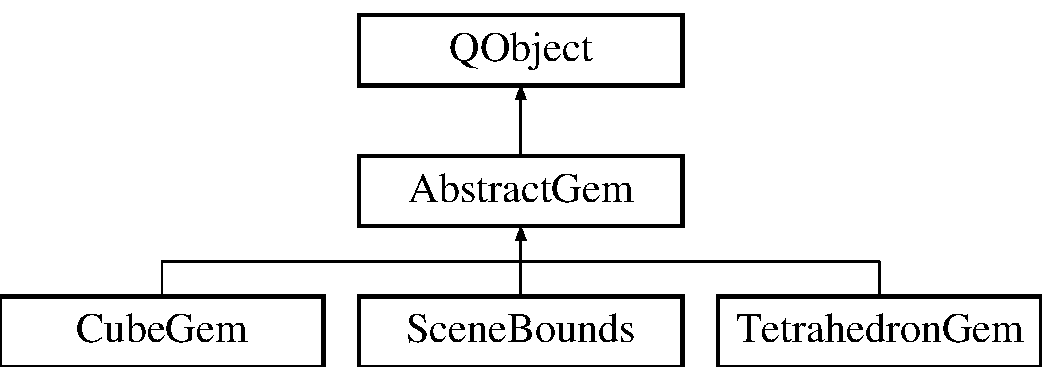
\includegraphics[height=3.000000cm]{class_abstract_gem}
\end{center}
\end{figure}
\subsection*{Public Slots}
\begin{DoxyCompactItemize}
\item 
void \hyperlink{class_abstract_gem_a6198aae1f2f54d73a7a5e66ca60f5f67}{set\+Rotation\+From\+Euler} (const Q\+Vector3\+D \&euler\+Rotation)
\begin{DoxyCompactList}\small\item\em Sets rotation of gem using euler angles. This method is mainly used to set initial rotation. \end{DoxyCompactList}\end{DoxyCompactItemize}
\subsection*{Signals}
\begin{DoxyCompactItemize}
\item 
void \hyperlink{class_abstract_gem_ac84dd4c9b3ea3adf02c1bfa74a29b649}{position\+Changed} ()
\item 
void \hyperlink{class_abstract_gem_a2702e870321deb40a8f056c1fce01094}{rotation\+Changed} ()
\item 
void \hyperlink{class_abstract_gem_a7e6bfe659f09bc68222211a58c365177}{scale\+Changed} ()
\item 
void \hyperlink{class_abstract_gem_ae20ad53d4ddeff9fc13878e7db5a3253}{color\+Changed} ()
\end{DoxyCompactItemize}
\subsection*{Public Member Functions}
\begin{DoxyCompactItemize}
\item 
\hyperlink{class_abstract_gem_a489d032060a42a9a8475309105fc585d}{Abstract\+Gem} (Q\+Object $\ast$parent=0)
\item 
virtual \hyperlink{class_abstract_gem_aafe5a4fa8c354ee562602d7b9ff1656b}{$\sim$\+Abstract\+Gem} ()
\item 
const Q\+Vector3\+D \& \hyperlink{class_abstract_gem_abb92885bcf86f43f069c9a0ef203d770}{color} () const 
\item 
void \hyperlink{class_abstract_gem_ace63416f61034b73969b5a89e3913e6d}{set\+Color} (const Q\+Vector3\+D \&\hyperlink{class_abstract_gem_ae73e6ac2448549460fbc597354ab0854}{color})
\item 
const \hyperlink{class_gem_data}{Gem\+Data} \& \hyperlink{class_abstract_gem_ac23fb212f3cca79b345f82e19f8c12d5}{data} () const 
\begin{DoxyCompactList}\small\item\em This method returns the \hyperlink{class_gem_data}{Gem\+Data} object describing the gem.  This method was not intended to be public, but we needed it for rendering. \end{DoxyCompactList}\item 
const Q\+Matrix4x4 \& \hyperlink{class_abstract_gem_a89f90d07bc8a780f053b3c6a5720aeed}{model} () const 
\begin{DoxyCompactList}\small\item\em Constructs normal matrix for gem in order to transform it from objectspace into worldsapce. \end{DoxyCompactList}\item 
const Q\+Vector3\+D \& \hyperlink{class_abstract_gem_a404114854610011363f6d7800985b718}{position} () const 
\item 
virtual void \hyperlink{class_abstract_gem_aaf11fa4b522dc334ebed4f2d031a3e2b}{set\+Position} (const Q\+Vector3\+D \&\hyperlink{class_abstract_gem_accd665898ada9bc95c886bfbcf56d9a8}{position})
\item 
qreal \hyperlink{class_abstract_gem_a628481ed4ebff7b282524a003d4392c2}{radius} () const 
\begin{DoxyCompactList}\small\item\em Radius of boundingsphere. This value is influenced by scale and the geometry of gem. \end{DoxyCompactList}\item 
const Q\+Quaternion \& \hyperlink{class_abstract_gem_a4fc9d6ed418b73ec2539e063ebfa70c1}{rotation} () const 
\begin{DoxyCompactList}\small\item\em Rotation around the own center. \end{DoxyCompactList}\item 
virtual void \hyperlink{class_abstract_gem_afce4d09f74fec117d27b11a220eee6b9}{set\+Rotation} (const Q\+Quaternion \&\hyperlink{class_abstract_gem_a6d85928549d64d369864716dbe2c716b}{rotation})
\begin{DoxyCompactList}\small\item\em Sets the rotation of gem around own center. \end{DoxyCompactList}\item 
void \hyperlink{class_abstract_gem_a5ca6867a835dfe2b49d46dbfb933bfca}{rotate} (const Q\+Quaternion \&quaternion)
\begin{DoxyCompactList}\small\item\em Rotates the gem around the center of the gem. \end{DoxyCompactList}\item 
qreal \hyperlink{class_abstract_gem_aadc1c5925331b573d9aba6c2451c9348}{scale} () const 
\item 
void \hyperlink{class_abstract_gem_a23693f4ebb5260cb21141bbcf3f4ff83}{set\+Scale} (qreal scale\+Factor)
\item 
\hyperlink{abstractgem_8h_a2f0a34b6dac35a9610cab7a1c5fcb444}{Gem\+Type} \hyperlink{class_abstract_gem_a4860dda50d7acab4f507505369da19f8}{type} () const 
\begin{DoxyCompactList}\small\item\em Returns the type of gem, in order to differntiate between types even you have only Abstract\+Gems. \end{DoxyCompactList}\item 
float \hyperlink{class_abstract_gem_a9f945c4f1b76ae90414ed3229d01dd0b}{bounding\+Sphere\+Intersected\+By} (const \hyperlink{class_light_ray}{Light\+Ray} \&ray, Q\+Vector3\+D $\ast$collision\+Point=nullptr)
\begin{DoxyCompactList}\small\item\em Calculates distance to collision with gems boundingsphere.  The boundingsphere is specified by gems themself and cannot be influenced from outside. Because the collision point is only calculated with the bondingsphere computation is pretty fast. \end{DoxyCompactList}\item 
virtual float \hyperlink{class_abstract_gem_adc52cc6d78f3494563c50cfd7e0584b4}{intersected\+By} (const \hyperlink{class_light_ray}{Light\+Ray} \&ray, Q\+Vector3\+D $\ast$collision\+Point=nullptr)
\begin{DoxyCompactList}\small\item\em Calcualtes the distance to collision of ray with gem.  This method calculates the real collision point therefor many computations are done especially for complex gems. \end{DoxyCompactList}\item 
virtual \hyperlink{class_q_list}{Q\+List}$<$ \hyperlink{class_light_ray}{Light\+Ray} $\ast$ $>$ \hyperlink{class_abstract_gem_ab4f3c6d38acbe59a610c67588e4944d7}{process\+Ray\+Intersection} (const \hyperlink{class_light_ray}{Light\+Ray} \&ray, \hyperlink{class_scene}{Scene} $\ast$scene)
\begin{DoxyCompactList}\small\item\em Calculates all new rays, that will be created by a collision with that gem. Also affect gem attributes. \end{DoxyCompactList}\end{DoxyCompactItemize}
\subsection*{Protected Member Functions}
\begin{DoxyCompactItemize}
\item 
int \hyperlink{class_abstract_gem_a85e872137d38a2c4a9a38f1f0b996bdc}{solve\+Quadric\+Formula} (float a, float b, float c, float \&x1, float \&x2)
\item 
float \hyperlink{class_abstract_gem_a446d8e7a7296203789414ae5b93e0bde}{face\+Intersected\+By} (const \hyperlink{class_light_ray}{Light\+Ray} \&ray, \hyperlink{class_triangle}{Triangle} $\ast$\&intersected\+Face, Q\+Vector3\+D $\ast$collision\+Point=nullptr)
\begin{DoxyCompactList}\small\item\em Finds face of gem intersected by given ray. Ownership of returned face is transfered to caller. \end{DoxyCompactList}\item 
\hyperlink{class_triangle}{Triangle} \hyperlink{class_abstract_gem_a18523ca4a999d5159e38003b3fad5f20}{in\+World\+Coordinates} (const \hyperlink{class_triangle}{Triangle} \&triangle)
\begin{DoxyCompactList}\small\item\em Calculates triangle in world coordinates for given triangle. Therefor position, rotatition and scale of gem are used. \end{DoxyCompactList}\end{DoxyCompactItemize}
\subsection*{Protected Attributes}
\begin{DoxyCompactItemize}
\item 
\hyperlink{class_gem_data}{Gem\+Data} $\ast$ \hyperlink{class_abstract_gem_a10a337f732ade69f1988659852f837c6}{m\+\_\+data}
\item 
qreal \hyperlink{class_abstract_gem_ab058af121fa66616cab7551e9418048a}{m\+\_\+radius}
\end{DoxyCompactItemize}
\subsection*{Properties}
\begin{DoxyCompactItemize}
\item 
const Q\+Vector3\+D \hyperlink{class_abstract_gem_accd665898ada9bc95c886bfbcf56d9a8}{position}
\item 
const Q\+Quaternion \hyperlink{class_abstract_gem_a6d85928549d64d369864716dbe2c716b}{rotation}
\item 
qreal \hyperlink{class_abstract_gem_a71c3b2720a5e3da61741f9043427ab51}{scale}
\item 
const Q\+Vector3\+D \hyperlink{class_abstract_gem_ae73e6ac2448549460fbc597354ab0854}{color}
\end{DoxyCompactItemize}


\subsection{Detailed Description}
The \hyperlink{class_abstract_gem}{Abstract\+Gem} class is our base class of all gems.  As base class all required information of a gem are stored. Also usefull algorithms for collision detection are provided. Furthermore this class is supposed to be used within Q\+M\+L. 

\subsection{Constructor \& Destructor Documentation}
\hypertarget{class_abstract_gem_a489d032060a42a9a8475309105fc585d}{}\index{Abstract\+Gem@{Abstract\+Gem}!Abstract\+Gem@{Abstract\+Gem}}
\index{Abstract\+Gem@{Abstract\+Gem}!Abstract\+Gem@{Abstract\+Gem}}
\subsubsection[{Abstract\+Gem}]{\setlength{\rightskip}{0pt plus 5cm}Abstract\+Gem\+::\+Abstract\+Gem (
\begin{DoxyParamCaption}
\item[{Q\+Object $\ast$}]{parent = {\ttfamily 0}}
\end{DoxyParamCaption}
)\hspace{0.3cm}{\ttfamily [explicit]}}\label{class_abstract_gem_a489d032060a42a9a8475309105fc585d}
\hypertarget{class_abstract_gem_aafe5a4fa8c354ee562602d7b9ff1656b}{}\index{Abstract\+Gem@{Abstract\+Gem}!````~Abstract\+Gem@{$\sim$\+Abstract\+Gem}}
\index{````~Abstract\+Gem@{$\sim$\+Abstract\+Gem}!Abstract\+Gem@{Abstract\+Gem}}
\subsubsection[{$\sim$\+Abstract\+Gem}]{\setlength{\rightskip}{0pt plus 5cm}Abstract\+Gem\+::$\sim$\+Abstract\+Gem (
\begin{DoxyParamCaption}
{}
\end{DoxyParamCaption}
)\hspace{0.3cm}{\ttfamily [virtual]}}\label{class_abstract_gem_aafe5a4fa8c354ee562602d7b9ff1656b}


\subsection{Member Function Documentation}
\hypertarget{class_abstract_gem_a9f945c4f1b76ae90414ed3229d01dd0b}{}\index{Abstract\+Gem@{Abstract\+Gem}!bounding\+Sphere\+Intersected\+By@{bounding\+Sphere\+Intersected\+By}}
\index{bounding\+Sphere\+Intersected\+By@{bounding\+Sphere\+Intersected\+By}!Abstract\+Gem@{Abstract\+Gem}}
\subsubsection[{bounding\+Sphere\+Intersected\+By}]{\setlength{\rightskip}{0pt plus 5cm}float Abstract\+Gem\+::bounding\+Sphere\+Intersected\+By (
\begin{DoxyParamCaption}
\item[{const {\bf Light\+Ray} \&}]{ray, }
\item[{Q\+Vector3\+D $\ast$}]{collision\+Point = {\ttfamily nullptr}}
\end{DoxyParamCaption}
)}\label{class_abstract_gem_a9f945c4f1b76ae90414ed3229d01dd0b}


Calculates distance to collision with gems boundingsphere.  The boundingsphere is specified by gems themself and cannot be influenced from outside. Because the collision point is only calculated with the bondingsphere computation is pretty fast. 


\begin{DoxyParams}{Parameters}
{\em ray} & The ray which might collide with gems boundingsphere \\
\hline
{\em collision\+Point} & Optional parameter. If provided the collision point of ray with boundingsphere is written into. If no collision occurs the maximum float value is wriiten into all components. \\
\hline
\end{DoxyParams}
\begin{DoxyReturn}{Returns}
The factor you need to apply ray.\+direction() to ray.\+start\+Position(). If no collision occurs maximum float value is returned. Do not compare this value with return values of \hyperlink{class_abstract_gem_adc52cc6d78f3494563c50cfd7e0584b4}{intersected\+By()}  \hyperlink{class_abstract_gem_adc52cc6d78f3494563c50cfd7e0584b4}{intersected\+By()} 
\end{DoxyReturn}
\hypertarget{class_abstract_gem_abb92885bcf86f43f069c9a0ef203d770}{}\index{Abstract\+Gem@{Abstract\+Gem}!color@{color}}
\index{color@{color}!Abstract\+Gem@{Abstract\+Gem}}
\subsubsection[{color}]{\setlength{\rightskip}{0pt plus 5cm}const Q\+Vector3\+D\& Abstract\+Gem\+::color (
\begin{DoxyParamCaption}
{}
\end{DoxyParamCaption}
) const}\label{class_abstract_gem_abb92885bcf86f43f069c9a0ef203d770}
\hypertarget{class_abstract_gem_ae20ad53d4ddeff9fc13878e7db5a3253}{}\index{Abstract\+Gem@{Abstract\+Gem}!color\+Changed@{color\+Changed}}
\index{color\+Changed@{color\+Changed}!Abstract\+Gem@{Abstract\+Gem}}
\subsubsection[{color\+Changed}]{\setlength{\rightskip}{0pt plus 5cm}void Abstract\+Gem\+::color\+Changed (
\begin{DoxyParamCaption}
{}
\end{DoxyParamCaption}
)\hspace{0.3cm}{\ttfamily [signal]}}\label{class_abstract_gem_ae20ad53d4ddeff9fc13878e7db5a3253}
\hypertarget{class_abstract_gem_ac23fb212f3cca79b345f82e19f8c12d5}{}\index{Abstract\+Gem@{Abstract\+Gem}!data@{data}}
\index{data@{data}!Abstract\+Gem@{Abstract\+Gem}}
\subsubsection[{data}]{\setlength{\rightskip}{0pt plus 5cm}const {\bf Gem\+Data} \& Abstract\+Gem\+::data (
\begin{DoxyParamCaption}
{}
\end{DoxyParamCaption}
) const}\label{class_abstract_gem_ac23fb212f3cca79b345f82e19f8c12d5}


This method returns the \hyperlink{class_gem_data}{Gem\+Data} object describing the gem.  This method was not intended to be public, but we needed it for rendering. 

\begin{DoxyReturn}{Returns}

\end{DoxyReturn}
\hypertarget{class_abstract_gem_a446d8e7a7296203789414ae5b93e0bde}{}\index{Abstract\+Gem@{Abstract\+Gem}!face\+Intersected\+By@{face\+Intersected\+By}}
\index{face\+Intersected\+By@{face\+Intersected\+By}!Abstract\+Gem@{Abstract\+Gem}}
\subsubsection[{face\+Intersected\+By}]{\setlength{\rightskip}{0pt plus 5cm}float Abstract\+Gem\+::face\+Intersected\+By (
\begin{DoxyParamCaption}
\item[{const {\bf Light\+Ray} \&}]{ray, }
\item[{{\bf Triangle} $\ast$\&}]{intersected\+Face, }
\item[{Q\+Vector3\+D $\ast$}]{collision\+Point = {\ttfamily nullptr}}
\end{DoxyParamCaption}
)\hspace{0.3cm}{\ttfamily [protected]}}\label{class_abstract_gem_a446d8e7a7296203789414ae5b93e0bde}


Finds face of gem intersected by given ray. Ownership of returned face is transfered to caller. 


\begin{DoxyParams}{Parameters}
{\em ray} & Ray that might intersect gem \\
\hline
{\em intersected\+Face} & A pointer to intersected face is written into. Because this triangle is in worldspace and for performance reasons the ownership of face is transfered to caller. If ray does not intersect nullptr is written. \\
\hline
{\em collision\+Point} & Optional parameter. If the given pointer is not nullptr the collisionpoint is written into. \\
\hline
\end{DoxyParams}
\begin{DoxyReturn}{Returns}
Returns distance to collisionpoint. If no collission occured the value is maximum of float. 
\end{DoxyReturn}
\hypertarget{class_abstract_gem_adc52cc6d78f3494563c50cfd7e0584b4}{}\index{Abstract\+Gem@{Abstract\+Gem}!intersected\+By@{intersected\+By}}
\index{intersected\+By@{intersected\+By}!Abstract\+Gem@{Abstract\+Gem}}
\subsubsection[{intersected\+By}]{\setlength{\rightskip}{0pt plus 5cm}float Abstract\+Gem\+::intersected\+By (
\begin{DoxyParamCaption}
\item[{const {\bf Light\+Ray} \&}]{ray, }
\item[{Q\+Vector3\+D $\ast$}]{collision\+Point = {\ttfamily nullptr}}
\end{DoxyParamCaption}
)\hspace{0.3cm}{\ttfamily [virtual]}}\label{class_abstract_gem_adc52cc6d78f3494563c50cfd7e0584b4}


Calcualtes the distance to collision of ray with gem.  This method calculates the real collision point therefor many computations are done especially for complex gems. 


\begin{DoxyParams}{Parameters}
{\em ray} & The ray that might collide with gem. \\
\hline
{\em collision\+Point} & Optional parameter. If a collision occurs the collision point will be written into this else all components contain maximum float values. \\
\hline
\end{DoxyParams}
\begin{DoxyReturn}{Returns}
The factor you need to apply ray.\+normalized\+Direction() to ray.\+start\+Direction(). If no collision occurs this value will be highest possible float. Do not compare this vale with return value of boundingsphere\+Intersected\+By()  \hyperlink{class_abstract_gem_a9f945c4f1b76ae90414ed3229d01dd0b}{bounding\+Sphere\+Intersected\+By()} 
\end{DoxyReturn}
\hypertarget{class_abstract_gem_a18523ca4a999d5159e38003b3fad5f20}{}\index{Abstract\+Gem@{Abstract\+Gem}!in\+World\+Coordinates@{in\+World\+Coordinates}}
\index{in\+World\+Coordinates@{in\+World\+Coordinates}!Abstract\+Gem@{Abstract\+Gem}}
\subsubsection[{in\+World\+Coordinates}]{\setlength{\rightskip}{0pt plus 5cm}{\bf Triangle} Abstract\+Gem\+::in\+World\+Coordinates (
\begin{DoxyParamCaption}
\item[{const {\bf Triangle} \&}]{triangle}
\end{DoxyParamCaption}
)\hspace{0.3cm}{\ttfamily [protected]}}\label{class_abstract_gem_a18523ca4a999d5159e38003b3fad5f20}


Calculates triangle in world coordinates for given triangle. Therefor position, rotatition and scale of gem are used. 


\begin{DoxyParams}{Parameters}
{\em triangle} & Objectspace triangle for wich the coressponding wolrdspace triangle should be calculated. \\
\hline
\end{DoxyParams}
\begin{DoxyReturn}{Returns}
Returns the \hyperlink{class_triangle}{Triangle} in wolrd coordinates, 
\end{DoxyReturn}
\hypertarget{class_abstract_gem_a89f90d07bc8a780f053b3c6a5720aeed}{}\index{Abstract\+Gem@{Abstract\+Gem}!model@{model}}
\index{model@{model}!Abstract\+Gem@{Abstract\+Gem}}
\subsubsection[{model}]{\setlength{\rightskip}{0pt plus 5cm}const Q\+Matrix4x4 \& Abstract\+Gem\+::model (
\begin{DoxyParamCaption}
{}
\end{DoxyParamCaption}
) const}\label{class_abstract_gem_a89f90d07bc8a780f053b3c6a5720aeed}


Constructs normal matrix for gem in order to transform it from objectspace into worldsapce. 

\begin{DoxyReturn}{Returns}

\end{DoxyReturn}
\hypertarget{class_abstract_gem_a404114854610011363f6d7800985b718}{}\index{Abstract\+Gem@{Abstract\+Gem}!position@{position}}
\index{position@{position}!Abstract\+Gem@{Abstract\+Gem}}
\subsubsection[{position}]{\setlength{\rightskip}{0pt plus 5cm}const Q\+Vector3\+D\& Abstract\+Gem\+::position (
\begin{DoxyParamCaption}
{}
\end{DoxyParamCaption}
) const}\label{class_abstract_gem_a404114854610011363f6d7800985b718}
\hypertarget{class_abstract_gem_ac84dd4c9b3ea3adf02c1bfa74a29b649}{}\index{Abstract\+Gem@{Abstract\+Gem}!position\+Changed@{position\+Changed}}
\index{position\+Changed@{position\+Changed}!Abstract\+Gem@{Abstract\+Gem}}
\subsubsection[{position\+Changed}]{\setlength{\rightskip}{0pt plus 5cm}void Abstract\+Gem\+::position\+Changed (
\begin{DoxyParamCaption}
{}
\end{DoxyParamCaption}
)\hspace{0.3cm}{\ttfamily [signal]}}\label{class_abstract_gem_ac84dd4c9b3ea3adf02c1bfa74a29b649}
\hypertarget{class_abstract_gem_ab4f3c6d38acbe59a610c67588e4944d7}{}\index{Abstract\+Gem@{Abstract\+Gem}!process\+Ray\+Intersection@{process\+Ray\+Intersection}}
\index{process\+Ray\+Intersection@{process\+Ray\+Intersection}!Abstract\+Gem@{Abstract\+Gem}}
\subsubsection[{process\+Ray\+Intersection}]{\setlength{\rightskip}{0pt plus 5cm}{\bf Q\+List}$<$ {\bf Light\+Ray} $\ast$ $>$ Abstract\+Gem\+::process\+Ray\+Intersection (
\begin{DoxyParamCaption}
\item[{const {\bf Light\+Ray} \&}]{ray, }
\item[{{\bf Scene} $\ast$}]{scene}
\end{DoxyParamCaption}
)\hspace{0.3cm}{\ttfamily [virtual]}}\label{class_abstract_gem_ab4f3c6d38acbe59a610c67588e4944d7}


Calculates all new rays, that will be created by a collision with that gem. Also affect gem attributes. 


\begin{DoxyParams}{Parameters}
{\em ray} & Ray that might collide. \\
\hline
{\em scene} & The scene the ray and gem are in. This is needed in order to calculate new rays appropraite. \\
\hline
\end{DoxyParams}
\begin{DoxyReturn}{Returns}
A List of lightrays that should be added to scene. If no collision occurs the list is empty. Ownership of rays contained in list is transfered to caller. 
\end{DoxyReturn}


Reimplemented in \hyperlink{class_scene_bounds_aeac6aafe6081e8efd6b4180e86346dc0}{Scene\+Bounds}.

\hypertarget{class_abstract_gem_a628481ed4ebff7b282524a003d4392c2}{}\index{Abstract\+Gem@{Abstract\+Gem}!radius@{radius}}
\index{radius@{radius}!Abstract\+Gem@{Abstract\+Gem}}
\subsubsection[{radius}]{\setlength{\rightskip}{0pt plus 5cm}qreal Abstract\+Gem\+::radius (
\begin{DoxyParamCaption}
{}
\end{DoxyParamCaption}
) const}\label{class_abstract_gem_a628481ed4ebff7b282524a003d4392c2}


Radius of boundingsphere. This value is influenced by scale and the geometry of gem. 

\begin{DoxyReturn}{Returns}

\end{DoxyReturn}
\hypertarget{class_abstract_gem_a5ca6867a835dfe2b49d46dbfb933bfca}{}\index{Abstract\+Gem@{Abstract\+Gem}!rotate@{rotate}}
\index{rotate@{rotate}!Abstract\+Gem@{Abstract\+Gem}}
\subsubsection[{rotate}]{\setlength{\rightskip}{0pt plus 5cm}void Abstract\+Gem\+::rotate (
\begin{DoxyParamCaption}
\item[{const Q\+Quaternion \&}]{quaternion}
\end{DoxyParamCaption}
)}\label{class_abstract_gem_a5ca6867a835dfe2b49d46dbfb933bfca}


Rotates the gem around the center of the gem. 


\begin{DoxyParams}{Parameters}
{\em quaternion} & Specifies how the gem should be rotated. \\
\hline
\end{DoxyParams}
\hypertarget{class_abstract_gem_a4fc9d6ed418b73ec2539e063ebfa70c1}{}\index{Abstract\+Gem@{Abstract\+Gem}!rotation@{rotation}}
\index{rotation@{rotation}!Abstract\+Gem@{Abstract\+Gem}}
\subsubsection[{rotation}]{\setlength{\rightskip}{0pt plus 5cm}const Q\+Quaternion\& Abstract\+Gem\+::rotation (
\begin{DoxyParamCaption}
{}
\end{DoxyParamCaption}
) const}\label{class_abstract_gem_a4fc9d6ed418b73ec2539e063ebfa70c1}


Rotation around the own center. 

\begin{DoxyReturn}{Returns}

\end{DoxyReturn}
\hypertarget{class_abstract_gem_a2702e870321deb40a8f056c1fce01094}{}\index{Abstract\+Gem@{Abstract\+Gem}!rotation\+Changed@{rotation\+Changed}}
\index{rotation\+Changed@{rotation\+Changed}!Abstract\+Gem@{Abstract\+Gem}}
\subsubsection[{rotation\+Changed}]{\setlength{\rightskip}{0pt plus 5cm}void Abstract\+Gem\+::rotation\+Changed (
\begin{DoxyParamCaption}
{}
\end{DoxyParamCaption}
)\hspace{0.3cm}{\ttfamily [signal]}}\label{class_abstract_gem_a2702e870321deb40a8f056c1fce01094}
\hypertarget{class_abstract_gem_aadc1c5925331b573d9aba6c2451c9348}{}\index{Abstract\+Gem@{Abstract\+Gem}!scale@{scale}}
\index{scale@{scale}!Abstract\+Gem@{Abstract\+Gem}}
\subsubsection[{scale}]{\setlength{\rightskip}{0pt plus 5cm}qreal Abstract\+Gem\+::scale (
\begin{DoxyParamCaption}
{}
\end{DoxyParamCaption}
) const}\label{class_abstract_gem_aadc1c5925331b573d9aba6c2451c9348}
\hypertarget{class_abstract_gem_a7e6bfe659f09bc68222211a58c365177}{}\index{Abstract\+Gem@{Abstract\+Gem}!scale\+Changed@{scale\+Changed}}
\index{scale\+Changed@{scale\+Changed}!Abstract\+Gem@{Abstract\+Gem}}
\subsubsection[{scale\+Changed}]{\setlength{\rightskip}{0pt plus 5cm}void Abstract\+Gem\+::scale\+Changed (
\begin{DoxyParamCaption}
{}
\end{DoxyParamCaption}
)\hspace{0.3cm}{\ttfamily [signal]}}\label{class_abstract_gem_a7e6bfe659f09bc68222211a58c365177}
\hypertarget{class_abstract_gem_ace63416f61034b73969b5a89e3913e6d}{}\index{Abstract\+Gem@{Abstract\+Gem}!set\+Color@{set\+Color}}
\index{set\+Color@{set\+Color}!Abstract\+Gem@{Abstract\+Gem}}
\subsubsection[{set\+Color}]{\setlength{\rightskip}{0pt plus 5cm}void Abstract\+Gem\+::set\+Color (
\begin{DoxyParamCaption}
\item[{const Q\+Vector3\+D \&}]{color}
\end{DoxyParamCaption}
)}\label{class_abstract_gem_ace63416f61034b73969b5a89e3913e6d}
\hypertarget{class_abstract_gem_aaf11fa4b522dc334ebed4f2d031a3e2b}{}\index{Abstract\+Gem@{Abstract\+Gem}!set\+Position@{set\+Position}}
\index{set\+Position@{set\+Position}!Abstract\+Gem@{Abstract\+Gem}}
\subsubsection[{set\+Position}]{\setlength{\rightskip}{0pt plus 5cm}void Abstract\+Gem\+::set\+Position (
\begin{DoxyParamCaption}
\item[{const Q\+Vector3\+D \&}]{position}
\end{DoxyParamCaption}
)\hspace{0.3cm}{\ttfamily [virtual]}}\label{class_abstract_gem_aaf11fa4b522dc334ebed4f2d031a3e2b}


Reimplemented in \hyperlink{class_scene_bounds_a26db5e7928d3ac7d0257dc52e1ed4e77}{Scene\+Bounds}.

\hypertarget{class_abstract_gem_afce4d09f74fec117d27b11a220eee6b9}{}\index{Abstract\+Gem@{Abstract\+Gem}!set\+Rotation@{set\+Rotation}}
\index{set\+Rotation@{set\+Rotation}!Abstract\+Gem@{Abstract\+Gem}}
\subsubsection[{set\+Rotation}]{\setlength{\rightskip}{0pt plus 5cm}void Abstract\+Gem\+::set\+Rotation (
\begin{DoxyParamCaption}
\item[{const Q\+Quaternion \&}]{rotation}
\end{DoxyParamCaption}
)\hspace{0.3cm}{\ttfamily [virtual]}}\label{class_abstract_gem_afce4d09f74fec117d27b11a220eee6b9}


Sets the rotation of gem around own center. 


\begin{DoxyParams}{Parameters}
{\em rotation} & Value the roation will be set to.  \hyperlink{class_abstract_gem_a6198aae1f2f54d73a7a5e66ca60f5f67}{set\+Rotation\+From\+Euler()} \\
\hline
\end{DoxyParams}


Reimplemented in \hyperlink{class_scene_bounds_a2e7b2f2e66700b414584ca6b407faf72}{Scene\+Bounds}.

\hypertarget{class_abstract_gem_a6198aae1f2f54d73a7a5e66ca60f5f67}{}\index{Abstract\+Gem@{Abstract\+Gem}!set\+Rotation\+From\+Euler@{set\+Rotation\+From\+Euler}}
\index{set\+Rotation\+From\+Euler@{set\+Rotation\+From\+Euler}!Abstract\+Gem@{Abstract\+Gem}}
\subsubsection[{set\+Rotation\+From\+Euler}]{\setlength{\rightskip}{0pt plus 5cm}void Abstract\+Gem\+::set\+Rotation\+From\+Euler (
\begin{DoxyParamCaption}
\item[{const Q\+Vector3\+D \&}]{euler\+Rotation}
\end{DoxyParamCaption}
)\hspace{0.3cm}{\ttfamily [slot]}}\label{class_abstract_gem_a6198aae1f2f54d73a7a5e66ca60f5f67}


Sets rotation of gem using euler angles. This method is mainly used to set initial rotation. 


\begin{DoxyParams}{Parameters}
{\em euler\+Rotation} & Q\+Vector3\+D containing the euler angles. The member of euler\+Vector contains corresponding rotation along axis (x component = rotation around x axis). The angle around axis is specified in degrees. \\
\hline
\end{DoxyParams}
\hypertarget{class_abstract_gem_a23693f4ebb5260cb21141bbcf3f4ff83}{}\index{Abstract\+Gem@{Abstract\+Gem}!set\+Scale@{set\+Scale}}
\index{set\+Scale@{set\+Scale}!Abstract\+Gem@{Abstract\+Gem}}
\subsubsection[{set\+Scale}]{\setlength{\rightskip}{0pt plus 5cm}void Abstract\+Gem\+::set\+Scale (
\begin{DoxyParamCaption}
\item[{qreal}]{scale\+Factor}
\end{DoxyParamCaption}
)}\label{class_abstract_gem_a23693f4ebb5260cb21141bbcf3f4ff83}
\hypertarget{class_abstract_gem_a85e872137d38a2c4a9a38f1f0b996bdc}{}\index{Abstract\+Gem@{Abstract\+Gem}!solve\+Quadric\+Formula@{solve\+Quadric\+Formula}}
\index{solve\+Quadric\+Formula@{solve\+Quadric\+Formula}!Abstract\+Gem@{Abstract\+Gem}}
\subsubsection[{solve\+Quadric\+Formula}]{\setlength{\rightskip}{0pt plus 5cm}int Abstract\+Gem\+::solve\+Quadric\+Formula (
\begin{DoxyParamCaption}
\item[{float}]{a, }
\item[{float}]{b, }
\item[{float}]{c, }
\item[{float \&}]{x1, }
\item[{float \&}]{x2}
\end{DoxyParamCaption}
)\hspace{0.3cm}{\ttfamily [protected]}}\label{class_abstract_gem_a85e872137d38a2c4a9a38f1f0b996bdc}
\hypertarget{class_abstract_gem_a4860dda50d7acab4f507505369da19f8}{}\index{Abstract\+Gem@{Abstract\+Gem}!type@{type}}
\index{type@{type}!Abstract\+Gem@{Abstract\+Gem}}
\subsubsection[{type}]{\setlength{\rightskip}{0pt plus 5cm}{\bf Gem\+Type} Abstract\+Gem\+::type (
\begin{DoxyParamCaption}
{}
\end{DoxyParamCaption}
) const}\label{class_abstract_gem_a4860dda50d7acab4f507505369da19f8}


Returns the type of gem, in order to differntiate between types even you have only Abstract\+Gems. 

\begin{DoxyReturn}{Returns}

\end{DoxyReturn}


\subsection{Member Data Documentation}
\hypertarget{class_abstract_gem_a10a337f732ade69f1988659852f837c6}{}\index{Abstract\+Gem@{Abstract\+Gem}!m\+\_\+data@{m\+\_\+data}}
\index{m\+\_\+data@{m\+\_\+data}!Abstract\+Gem@{Abstract\+Gem}}
\subsubsection[{m\+\_\+data}]{\setlength{\rightskip}{0pt plus 5cm}{\bf Gem\+Data}$\ast$ Abstract\+Gem\+::m\+\_\+data\hspace{0.3cm}{\ttfamily [protected]}}\label{class_abstract_gem_a10a337f732ade69f1988659852f837c6}
\hypertarget{class_abstract_gem_ab058af121fa66616cab7551e9418048a}{}\index{Abstract\+Gem@{Abstract\+Gem}!m\+\_\+radius@{m\+\_\+radius}}
\index{m\+\_\+radius@{m\+\_\+radius}!Abstract\+Gem@{Abstract\+Gem}}
\subsubsection[{m\+\_\+radius}]{\setlength{\rightskip}{0pt plus 5cm}qreal Abstract\+Gem\+::m\+\_\+radius\hspace{0.3cm}{\ttfamily [protected]}}\label{class_abstract_gem_ab058af121fa66616cab7551e9418048a}


\subsection{Property Documentation}
\hypertarget{class_abstract_gem_ae73e6ac2448549460fbc597354ab0854}{}\index{Abstract\+Gem@{Abstract\+Gem}!color@{color}}
\index{color@{color}!Abstract\+Gem@{Abstract\+Gem}}
\subsubsection[{color}]{\setlength{\rightskip}{0pt plus 5cm}const Q\+Vector3\+D \& Abstract\+Gem\+::color\hspace{0.3cm}{\ttfamily [read]}, {\ttfamily [write]}}\label{class_abstract_gem_ae73e6ac2448549460fbc597354ab0854}
\hypertarget{class_abstract_gem_accd665898ada9bc95c886bfbcf56d9a8}{}\index{Abstract\+Gem@{Abstract\+Gem}!position@{position}}
\index{position@{position}!Abstract\+Gem@{Abstract\+Gem}}
\subsubsection[{position}]{\setlength{\rightskip}{0pt plus 5cm}const Q\+Vector3\+D \& Abstract\+Gem\+::position\hspace{0.3cm}{\ttfamily [read]}, {\ttfamily [write]}}\label{class_abstract_gem_accd665898ada9bc95c886bfbcf56d9a8}
\hypertarget{class_abstract_gem_a6d85928549d64d369864716dbe2c716b}{}\index{Abstract\+Gem@{Abstract\+Gem}!rotation@{rotation}}
\index{rotation@{rotation}!Abstract\+Gem@{Abstract\+Gem}}
\subsubsection[{rotation}]{\setlength{\rightskip}{0pt plus 5cm}const Q\+Quaternion \& Abstract\+Gem\+::rotation\hspace{0.3cm}{\ttfamily [read]}, {\ttfamily [write]}}\label{class_abstract_gem_a6d85928549d64d369864716dbe2c716b}
\hypertarget{class_abstract_gem_a71c3b2720a5e3da61741f9043427ab51}{}\index{Abstract\+Gem@{Abstract\+Gem}!scale@{scale}}
\index{scale@{scale}!Abstract\+Gem@{Abstract\+Gem}}
\subsubsection[{scale}]{\setlength{\rightskip}{0pt plus 5cm}qreal Abstract\+Gem\+::scale\hspace{0.3cm}{\ttfamily [read]}, {\ttfamily [write]}}\label{class_abstract_gem_a71c3b2720a5e3da61741f9043427ab51}


The documentation for this class was generated from the following files\+:\begin{DoxyCompactItemize}
\item 
Game-\/\+Programming-\/\+W\+S2014/gem\+Illuminator/\hyperlink{abstractgem_8h}{abstractgem.\+h}\item 
Game-\/\+Programming-\/\+W\+S2014/gem\+Illuminator/\hyperlink{abstractgem_8cpp}{abstractgem.\+cpp}\end{DoxyCompactItemize}

\hypertarget{class_blur_effect}{}\section{Blur\+Effect Class Reference}
\label{class_blur_effect}\index{Blur\+Effect@{Blur\+Effect}}


The \hyperlink{class_blur_effect}{Blur\+Effect} blurs a given texture.  




{\ttfamily \#include $<$blureffect.\+h$>$}

Inheritance diagram for Blur\+Effect\+:\begin{figure}[H]
\begin{center}
\leavevmode
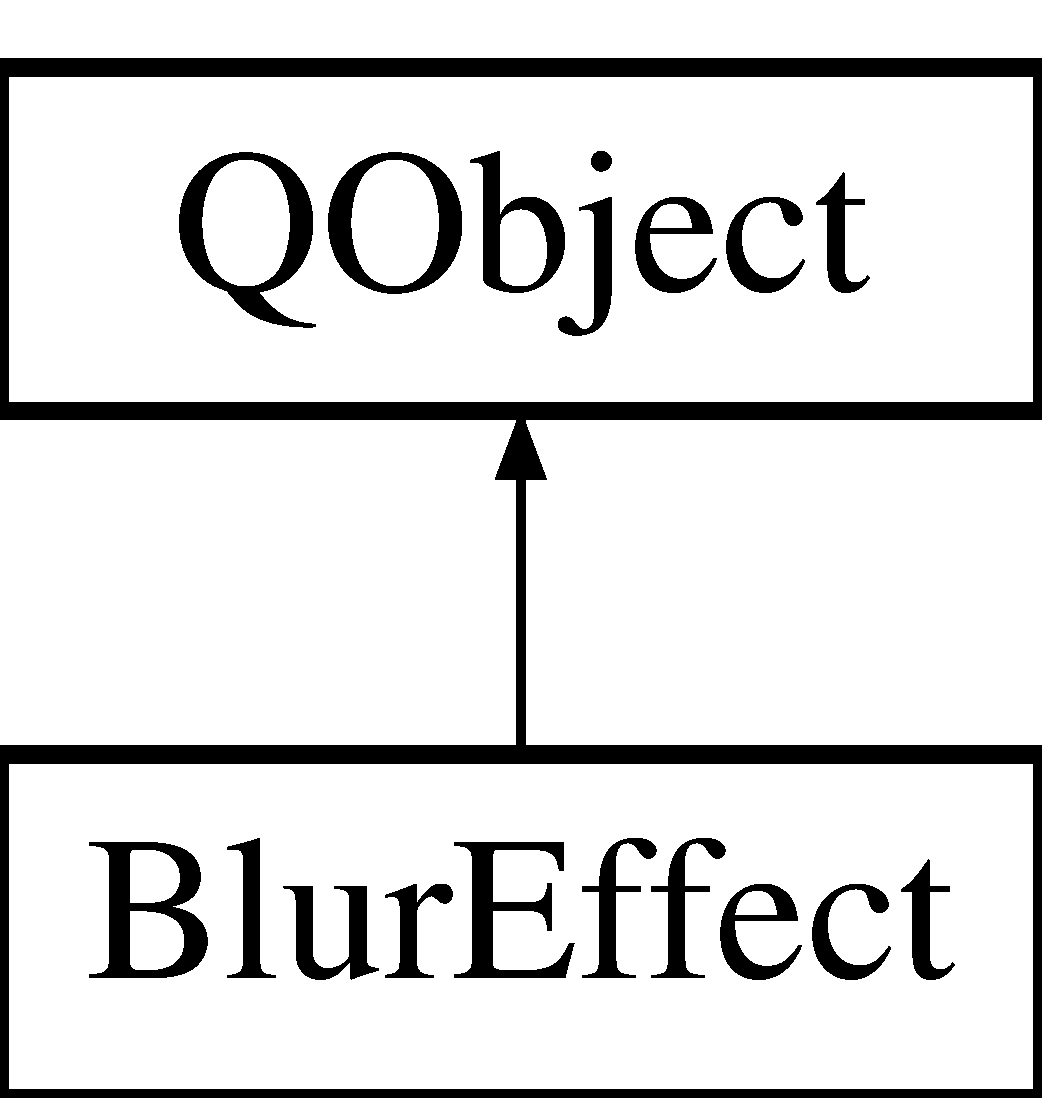
\includegraphics[height=2.000000cm]{class_blur_effect}
\end{center}
\end{figure}
\subsection*{Public Member Functions}
\begin{DoxyCompactItemize}
\item 
\hyperlink{class_blur_effect_a3653fdf73228f64b5fab03589060c704}{Blur\+Effect} (Q\+Open\+G\+L\+Functions \&gl, uint glow\+Texture, Q\+Object $\ast$parent=nullptr)
\begin{DoxyCompactList}\small\item\em Creates a new \hyperlink{class_blur_effect}{Blur\+Effect}, that will blur a specified texture everytime \hyperlink{class_blur_effect_a0317d7ce7078d1e28e7e5b37fb60b9f3}{blur()} is called. \end{DoxyCompactList}\item 
virtual \hyperlink{class_blur_effect_aeb30b45dd769774ff0f0706a4ad6566c}{$\sim$\+Blur\+Effect} ()
\item 
void \hyperlink{class_blur_effect_a0317d7ce7078d1e28e7e5b37fb60b9f3}{blur} (const Q\+Size \&texture\+Size)
\begin{DoxyCompactList}\small\item\em Blurs previous set texture.  The texture is blurred using two seperated passes of gauss blur. The result is a gaussblur with 9x9 kernel. \end{DoxyCompactList}\end{DoxyCompactItemize}
\subsection*{Protected Member Functions}
\begin{DoxyCompactItemize}
\item 
void \hyperlink{class_blur_effect_a735fa8b4020353e440d226e3a48a9e46}{initialize} ()
\item 
void \hyperlink{class_blur_effect_a673b5ec9a6f4a32bc0bab462b32c7200}{initialize\+F\+B\+Os} ()
\item 
void \hyperlink{class_blur_effect_a3acf8584853e2a2befdbb69eeb65aa2a}{initialize\+Shader\+Programs} ()
\item 
void \hyperlink{class_blur_effect_ad25107035e2585492d3501d8d2d51aa2}{render\+Gauss\+Horizontal} (const Q\+Size \&texture\+Size)
\begin{DoxyCompactList}\small\item\em Blurs texture horizontally. \end{DoxyCompactList}\item 
void \hyperlink{class_blur_effect_aaaaec0e2eb4530834e7ab3ad8beec231}{render\+Gauss\+Vertical} (const Q\+Size \&texture\+Size)
\begin{DoxyCompactList}\small\item\em Blurs texture vertically. \end{DoxyCompactList}\end{DoxyCompactItemize}
\subsection*{Protected Attributes}
\begin{DoxyCompactItemize}
\item 
Q\+Open\+G\+L\+Functions \& \hyperlink{class_blur_effect_a60e476bb206ce650162006e19891f4e2}{m\+\_\+gl}
\item 
Q\+Map$<$ \hyperlink{shaderprograms_8h_ada89718f8d394b2cc093eb9770c554ff}{Shader\+Programs}, Q\+Open\+G\+L\+Shader\+Program $\ast$ $>$ $\ast$ \hyperlink{class_blur_effect_a36f1750676d9a4b935609300a2c8853c}{m\+\_\+shader\+Programs}
\item 
bool \hyperlink{class_blur_effect_abd260e17d64d3e819c9817e2ae92a33d}{m\+\_\+initialized}
\item 
uint \hyperlink{class_blur_effect_a3cf63e0dc804b038a9348923a5df12f5}{m\+\_\+blur\+F\+B\+O}
\item 
uint \hyperlink{class_blur_effect_a8d3832820bc3cf08171d449cc0dc9430}{m\+\_\+blur\+Texture}
\item 
uint \hyperlink{class_blur_effect_a8bcdeba40d4a73e06a02dc7507ed498e}{m\+\_\+secondary\+Blur\+F\+B\+O}
\item 
uint \hyperlink{class_blur_effect_a1e068c508f32617c867a92a56d521888}{m\+\_\+secondary\+Blur\+Texture}
\item 
Q\+Size $\ast$ \hyperlink{class_blur_effect_a8513aa58d2ff05cc6b135f60c25d0710}{m\+\_\+used\+Viewport}
\item 
\hyperlink{class_screen_aligned_quad}{Screen\+Aligned\+Quad} $\ast$ \hyperlink{class_blur_effect_aa5fb6e7e38f9548b89f7cc6e8de0882a}{m\+\_\+quad}
\end{DoxyCompactItemize}


\subsection{Detailed Description}
The \hyperlink{class_blur_effect}{Blur\+Effect} blurs a given texture. 

\subsection{Constructor \& Destructor Documentation}
\hypertarget{class_blur_effect_a3653fdf73228f64b5fab03589060c704}{}\index{Blur\+Effect@{Blur\+Effect}!Blur\+Effect@{Blur\+Effect}}
\index{Blur\+Effect@{Blur\+Effect}!Blur\+Effect@{Blur\+Effect}}
\subsubsection[{Blur\+Effect}]{\setlength{\rightskip}{0pt plus 5cm}Blur\+Effect\+::\+Blur\+Effect (
\begin{DoxyParamCaption}
\item[{Q\+Open\+G\+L\+Functions \&}]{gl, }
\item[{uint}]{glow\+Texture, }
\item[{Q\+Object $\ast$}]{parent = {\ttfamily nullptr}}
\end{DoxyParamCaption}
)}\label{class_blur_effect_a3653fdf73228f64b5fab03589060c704}


Creates a new \hyperlink{class_blur_effect}{Blur\+Effect}, that will blur a specified texture everytime \hyperlink{class_blur_effect_a0317d7ce7078d1e28e7e5b37fb60b9f3}{blur()} is called. 


\begin{DoxyParams}{Parameters}
{\em gl} & The Q\+Open\+G\+L\+Funtions will be used for all gl-\/calls. \\
\hline
{\em glow\+Texture} & The texture that will be blurred. \\
\hline
{\em parent} & Q\+Object-\/parent \\
\hline
\end{DoxyParams}
\hypertarget{class_blur_effect_aeb30b45dd769774ff0f0706a4ad6566c}{}\index{Blur\+Effect@{Blur\+Effect}!````~Blur\+Effect@{$\sim$\+Blur\+Effect}}
\index{````~Blur\+Effect@{$\sim$\+Blur\+Effect}!Blur\+Effect@{Blur\+Effect}}
\subsubsection[{$\sim$\+Blur\+Effect}]{\setlength{\rightskip}{0pt plus 5cm}Blur\+Effect\+::$\sim$\+Blur\+Effect (
\begin{DoxyParamCaption}
{}
\end{DoxyParamCaption}
)\hspace{0.3cm}{\ttfamily [virtual]}}\label{class_blur_effect_aeb30b45dd769774ff0f0706a4ad6566c}


\subsection{Member Function Documentation}
\hypertarget{class_blur_effect_a0317d7ce7078d1e28e7e5b37fb60b9f3}{}\index{Blur\+Effect@{Blur\+Effect}!blur@{blur}}
\index{blur@{blur}!Blur\+Effect@{Blur\+Effect}}
\subsubsection[{blur}]{\setlength{\rightskip}{0pt plus 5cm}void Blur\+Effect\+::blur (
\begin{DoxyParamCaption}
\item[{const Q\+Size \&}]{texture\+Size}
\end{DoxyParamCaption}
)}\label{class_blur_effect_a0317d7ce7078d1e28e7e5b37fb60b9f3}


Blurs previous set texture.  The texture is blurred using two seperated passes of gauss blur. The result is a gaussblur with 9x9 kernel. 


\begin{DoxyParams}{Parameters}
{\em texture\+Size} & The size of texture, because we support changing texture sizes. \\
\hline
\end{DoxyParams}
\hypertarget{class_blur_effect_a735fa8b4020353e440d226e3a48a9e46}{}\index{Blur\+Effect@{Blur\+Effect}!initialize@{initialize}}
\index{initialize@{initialize}!Blur\+Effect@{Blur\+Effect}}
\subsubsection[{initialize}]{\setlength{\rightskip}{0pt plus 5cm}void Blur\+Effect\+::initialize (
\begin{DoxyParamCaption}
{}
\end{DoxyParamCaption}
)\hspace{0.3cm}{\ttfamily [protected]}}\label{class_blur_effect_a735fa8b4020353e440d226e3a48a9e46}
\hypertarget{class_blur_effect_a673b5ec9a6f4a32bc0bab462b32c7200}{}\index{Blur\+Effect@{Blur\+Effect}!initialize\+F\+B\+Os@{initialize\+F\+B\+Os}}
\index{initialize\+F\+B\+Os@{initialize\+F\+B\+Os}!Blur\+Effect@{Blur\+Effect}}
\subsubsection[{initialize\+F\+B\+Os}]{\setlength{\rightskip}{0pt plus 5cm}void Blur\+Effect\+::initialize\+F\+B\+Os (
\begin{DoxyParamCaption}
{}
\end{DoxyParamCaption}
)\hspace{0.3cm}{\ttfamily [protected]}}\label{class_blur_effect_a673b5ec9a6f4a32bc0bab462b32c7200}
\hypertarget{class_blur_effect_a3acf8584853e2a2befdbb69eeb65aa2a}{}\index{Blur\+Effect@{Blur\+Effect}!initialize\+Shader\+Programs@{initialize\+Shader\+Programs}}
\index{initialize\+Shader\+Programs@{initialize\+Shader\+Programs}!Blur\+Effect@{Blur\+Effect}}
\subsubsection[{initialize\+Shader\+Programs}]{\setlength{\rightskip}{0pt plus 5cm}void Blur\+Effect\+::initialize\+Shader\+Programs (
\begin{DoxyParamCaption}
{}
\end{DoxyParamCaption}
)\hspace{0.3cm}{\ttfamily [protected]}}\label{class_blur_effect_a3acf8584853e2a2befdbb69eeb65aa2a}
\hypertarget{class_blur_effect_ad25107035e2585492d3501d8d2d51aa2}{}\index{Blur\+Effect@{Blur\+Effect}!render\+Gauss\+Horizontal@{render\+Gauss\+Horizontal}}
\index{render\+Gauss\+Horizontal@{render\+Gauss\+Horizontal}!Blur\+Effect@{Blur\+Effect}}
\subsubsection[{render\+Gauss\+Horizontal}]{\setlength{\rightskip}{0pt plus 5cm}void Blur\+Effect\+::render\+Gauss\+Horizontal (
\begin{DoxyParamCaption}
\item[{const Q\+Size \&}]{texture\+Size}
\end{DoxyParamCaption}
)\hspace{0.3cm}{\ttfamily [protected]}}\label{class_blur_effect_ad25107035e2585492d3501d8d2d51aa2}


Blurs texture horizontally. 


\begin{DoxyParams}{Parameters}
{\em texture\+Size} & The current size of texture that is blurred. \\
\hline
\end{DoxyParams}
\hypertarget{class_blur_effect_aaaaec0e2eb4530834e7ab3ad8beec231}{}\index{Blur\+Effect@{Blur\+Effect}!render\+Gauss\+Vertical@{render\+Gauss\+Vertical}}
\index{render\+Gauss\+Vertical@{render\+Gauss\+Vertical}!Blur\+Effect@{Blur\+Effect}}
\subsubsection[{render\+Gauss\+Vertical}]{\setlength{\rightskip}{0pt plus 5cm}void Blur\+Effect\+::render\+Gauss\+Vertical (
\begin{DoxyParamCaption}
\item[{const Q\+Size \&}]{texture\+Size}
\end{DoxyParamCaption}
)\hspace{0.3cm}{\ttfamily [protected]}}\label{class_blur_effect_aaaaec0e2eb4530834e7ab3ad8beec231}


Blurs texture vertically. 


\begin{DoxyParams}{Parameters}
{\em texture\+Size} & The current size of texture that is blurred. \\
\hline
\end{DoxyParams}


\subsection{Member Data Documentation}
\hypertarget{class_blur_effect_a3cf63e0dc804b038a9348923a5df12f5}{}\index{Blur\+Effect@{Blur\+Effect}!m\+\_\+blur\+F\+B\+O@{m\+\_\+blur\+F\+B\+O}}
\index{m\+\_\+blur\+F\+B\+O@{m\+\_\+blur\+F\+B\+O}!Blur\+Effect@{Blur\+Effect}}
\subsubsection[{m\+\_\+blur\+F\+B\+O}]{\setlength{\rightskip}{0pt plus 5cm}uint Blur\+Effect\+::m\+\_\+blur\+F\+B\+O\hspace{0.3cm}{\ttfamily [protected]}}\label{class_blur_effect_a3cf63e0dc804b038a9348923a5df12f5}
\hypertarget{class_blur_effect_a8d3832820bc3cf08171d449cc0dc9430}{}\index{Blur\+Effect@{Blur\+Effect}!m\+\_\+blur\+Texture@{m\+\_\+blur\+Texture}}
\index{m\+\_\+blur\+Texture@{m\+\_\+blur\+Texture}!Blur\+Effect@{Blur\+Effect}}
\subsubsection[{m\+\_\+blur\+Texture}]{\setlength{\rightskip}{0pt plus 5cm}uint Blur\+Effect\+::m\+\_\+blur\+Texture\hspace{0.3cm}{\ttfamily [protected]}}\label{class_blur_effect_a8d3832820bc3cf08171d449cc0dc9430}
\hypertarget{class_blur_effect_a60e476bb206ce650162006e19891f4e2}{}\index{Blur\+Effect@{Blur\+Effect}!m\+\_\+gl@{m\+\_\+gl}}
\index{m\+\_\+gl@{m\+\_\+gl}!Blur\+Effect@{Blur\+Effect}}
\subsubsection[{m\+\_\+gl}]{\setlength{\rightskip}{0pt plus 5cm}Q\+Open\+G\+L\+Functions\& Blur\+Effect\+::m\+\_\+gl\hspace{0.3cm}{\ttfamily [protected]}}\label{class_blur_effect_a60e476bb206ce650162006e19891f4e2}
\hypertarget{class_blur_effect_abd260e17d64d3e819c9817e2ae92a33d}{}\index{Blur\+Effect@{Blur\+Effect}!m\+\_\+initialized@{m\+\_\+initialized}}
\index{m\+\_\+initialized@{m\+\_\+initialized}!Blur\+Effect@{Blur\+Effect}}
\subsubsection[{m\+\_\+initialized}]{\setlength{\rightskip}{0pt plus 5cm}bool Blur\+Effect\+::m\+\_\+initialized\hspace{0.3cm}{\ttfamily [protected]}}\label{class_blur_effect_abd260e17d64d3e819c9817e2ae92a33d}
\hypertarget{class_blur_effect_aa5fb6e7e38f9548b89f7cc6e8de0882a}{}\index{Blur\+Effect@{Blur\+Effect}!m\+\_\+quad@{m\+\_\+quad}}
\index{m\+\_\+quad@{m\+\_\+quad}!Blur\+Effect@{Blur\+Effect}}
\subsubsection[{m\+\_\+quad}]{\setlength{\rightskip}{0pt plus 5cm}{\bf Screen\+Aligned\+Quad}$\ast$ Blur\+Effect\+::m\+\_\+quad\hspace{0.3cm}{\ttfamily [protected]}}\label{class_blur_effect_aa5fb6e7e38f9548b89f7cc6e8de0882a}
\hypertarget{class_blur_effect_a8bcdeba40d4a73e06a02dc7507ed498e}{}\index{Blur\+Effect@{Blur\+Effect}!m\+\_\+secondary\+Blur\+F\+B\+O@{m\+\_\+secondary\+Blur\+F\+B\+O}}
\index{m\+\_\+secondary\+Blur\+F\+B\+O@{m\+\_\+secondary\+Blur\+F\+B\+O}!Blur\+Effect@{Blur\+Effect}}
\subsubsection[{m\+\_\+secondary\+Blur\+F\+B\+O}]{\setlength{\rightskip}{0pt plus 5cm}uint Blur\+Effect\+::m\+\_\+secondary\+Blur\+F\+B\+O\hspace{0.3cm}{\ttfamily [protected]}}\label{class_blur_effect_a8bcdeba40d4a73e06a02dc7507ed498e}
\hypertarget{class_blur_effect_a1e068c508f32617c867a92a56d521888}{}\index{Blur\+Effect@{Blur\+Effect}!m\+\_\+secondary\+Blur\+Texture@{m\+\_\+secondary\+Blur\+Texture}}
\index{m\+\_\+secondary\+Blur\+Texture@{m\+\_\+secondary\+Blur\+Texture}!Blur\+Effect@{Blur\+Effect}}
\subsubsection[{m\+\_\+secondary\+Blur\+Texture}]{\setlength{\rightskip}{0pt plus 5cm}uint Blur\+Effect\+::m\+\_\+secondary\+Blur\+Texture\hspace{0.3cm}{\ttfamily [protected]}}\label{class_blur_effect_a1e068c508f32617c867a92a56d521888}
\hypertarget{class_blur_effect_a36f1750676d9a4b935609300a2c8853c}{}\index{Blur\+Effect@{Blur\+Effect}!m\+\_\+shader\+Programs@{m\+\_\+shader\+Programs}}
\index{m\+\_\+shader\+Programs@{m\+\_\+shader\+Programs}!Blur\+Effect@{Blur\+Effect}}
\subsubsection[{m\+\_\+shader\+Programs}]{\setlength{\rightskip}{0pt plus 5cm}Q\+Map$<${\bf Shader\+Programs}, Q\+Open\+G\+L\+Shader\+Program$\ast$$>$$\ast$ Blur\+Effect\+::m\+\_\+shader\+Programs\hspace{0.3cm}{\ttfamily [protected]}}\label{class_blur_effect_a36f1750676d9a4b935609300a2c8853c}
\hypertarget{class_blur_effect_a8513aa58d2ff05cc6b135f60c25d0710}{}\index{Blur\+Effect@{Blur\+Effect}!m\+\_\+used\+Viewport@{m\+\_\+used\+Viewport}}
\index{m\+\_\+used\+Viewport@{m\+\_\+used\+Viewport}!Blur\+Effect@{Blur\+Effect}}
\subsubsection[{m\+\_\+used\+Viewport}]{\setlength{\rightskip}{0pt plus 5cm}Q\+Size$\ast$ Blur\+Effect\+::m\+\_\+used\+Viewport\hspace{0.3cm}{\ttfamily [protected]}}\label{class_blur_effect_a8513aa58d2ff05cc6b135f60c25d0710}


The documentation for this class was generated from the following files\+:\begin{DoxyCompactItemize}
\item 
Game-\/\+Programming-\/\+W\+S2014/gem\+Illuminator/\hyperlink{blureffect_8h}{blureffect.\+h}\item 
Game-\/\+Programming-\/\+W\+S2014/gem\+Illuminator/\hyperlink{blureffect_8cpp}{blureffect.\+cpp}\end{DoxyCompactItemize}

\hypertarget{class_camera}{}\section{Camera Class Reference}
\label{class_camera}\index{Camera@{Camera}}


The \hyperlink{class_camera}{Camera} class provides view and perspective projection matrices. Additional the viewport of camera is stored.  The view of camera has to be specified by eye, center and up or by position, viewdirection and up. It is allowed to mix both definitions, but it might lead to unexpected behaviour. The perspective projection is specified by field of view, viewport, and near and far plane.  




{\ttfamily \#include $<$camera.\+h$>$}

Inheritance diagram for Camera\+:\begin{figure}[H]
\begin{center}
\leavevmode
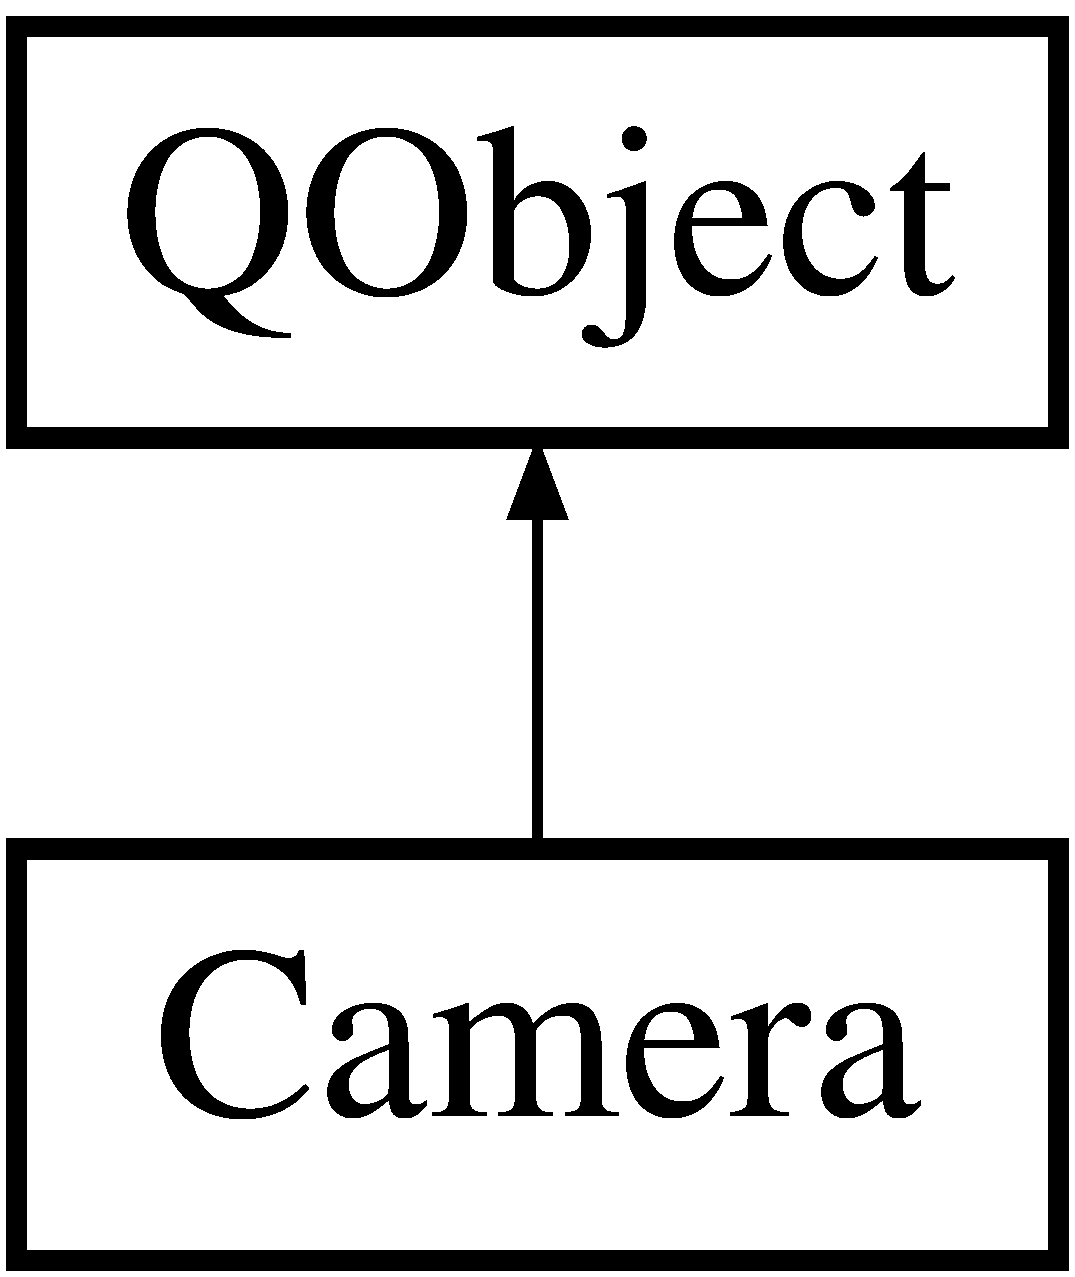
\includegraphics[height=2.000000cm]{class_camera}
\end{center}
\end{figure}
\subsection*{Public Slots}
\begin{DoxyCompactItemize}
\item 
void \hyperlink{class_camera_a3ac4fcd89c146068205a3c8b73a86520}{set\+Position} (const Q\+Vector3\+D \&\hyperlink{class_camera_a1e8c173f6a47c5ebea0e91aefea50b51}{position})
\begin{DoxyCompactList}\small\item\em Set position of camera to given value. \hyperlink{class_camera_aacb30cc51aef5e3f98db5b51e3a4ef3b}{center()} will be changed in order to keep \hyperlink{class_camera_a7745654f918533ddc5e285bcf630e934}{view\+Direction()} the same. \end{DoxyCompactList}\item 
void \hyperlink{class_camera_a61a059ce3aedc779f9087dda9b5e227c}{set\+View\+Direction} (const Q\+Vector3\+D \&\hyperlink{class_camera_a7745654f918533ddc5e285bcf630e934}{view\+Direction})
\begin{DoxyCompactList}\small\item\em Set view\+Direction of camera to given vector. \hyperlink{class_camera_aacb30cc51aef5e3f98db5b51e3a4ef3b}{center()} will be changed in order to. \end{DoxyCompactList}\item 
void \hyperlink{class_camera_aa445664f0bf5f3cd892a99125e4bc786}{set\+Eye} (const Q\+Vector3\+D \&\hyperlink{class_camera_aac5808300c4e00d266da238ad35b1a1b}{eye})
\begin{DoxyCompactList}\small\item\em Set eye (position) of camera to given value. \hyperlink{class_camera_aacb30cc51aef5e3f98db5b51e3a4ef3b}{center()} will not be changed, so \hyperlink{class_camera_a7745654f918533ddc5e285bcf630e934}{view\+Direction()} is set to \hyperlink{class_camera_aacb30cc51aef5e3f98db5b51e3a4ef3b}{center()} -\/ \hyperlink{class_camera_aac5808300c4e00d266da238ad35b1a1b}{eye()} \end{DoxyCompactList}\item 
void \hyperlink{class_camera_ae0594124b7a1baf13ef38de7a6bd0ed8}{set\+Center} (const Q\+Vector3\+D \&\hyperlink{class_camera_aacb30cc51aef5e3f98db5b51e3a4ef3b}{center})
\begin{DoxyCompactList}\small\item\em Set center of camera to given value. \hyperlink{class_camera_a7745654f918533ddc5e285bcf630e934}{view\+Direction()} will be set to new \hyperlink{class_camera_aacb30cc51aef5e3f98db5b51e3a4ef3b}{center()} -\/ \hyperlink{class_camera_aac5808300c4e00d266da238ad35b1a1b}{eye()}. \end{DoxyCompactList}\item 
void \hyperlink{class_camera_a037ef3f032c7fc09fa1f044260dd3a09}{set\+Up} (const Q\+Vector3\+D \&\hyperlink{class_camera_a86995a93a125a9d9941f10144c4c398e}{up})
\begin{DoxyCompactList}\small\item\em Set up-\/vector of camera. \end{DoxyCompactList}\item 
void \hyperlink{class_camera_a995075e3b619176b72ad2ff0ab434ed8}{set\+View} (const Q\+Vector3\+D \&\hyperlink{class_camera_aac5808300c4e00d266da238ad35b1a1b}{eye}, const Q\+Vector3\+D \&\hyperlink{class_camera_aacb30cc51aef5e3f98db5b51e3a4ef3b}{center}, const Q\+Vector3\+D \&\hyperlink{class_camera_a86995a93a125a9d9941f10144c4c398e}{up})
\begin{DoxyCompactList}\small\item\em Convinence method to specify view with one method call. \end{DoxyCompactList}\item 
void \hyperlink{class_camera_ad47041196bf35fed448003491112f528}{set\+Viewport} (const Q\+Size \&\hyperlink{class_camera_a56b601feb6a54eee0bce1910cdeac291}{viewport})
\item 
void \hyperlink{class_camera_ab0794a4ebc430368c5c3731e9bb35cdc}{set\+Viewport} (int x, int y)
\item 
void \hyperlink{class_camera_aa0e1d52fdb7e3d060041b960fa8b5c24}{set\+Fovy} (float angle)
\item 
void \hyperlink{class_camera_a4a8cda23fc022255f30452f608c66081}{set\+Z\+Near} (float \hyperlink{class_camera_a1db2166635ff27594eda3a23130b66ac}{z\+Near})
\item 
void \hyperlink{class_camera_a8ab94de2388acc72fa129fa203ccc587}{set\+Z\+Far} (float \hyperlink{class_camera_a6290469f972a5903c805725db563f41f}{z\+Far})
\end{DoxyCompactItemize}
\subsection*{Signals}
\begin{DoxyCompactItemize}
\item 
void \hyperlink{class_camera_af652ce7cb83eb966a90393be8e0038c3}{view\+Changed} ()
\end{DoxyCompactItemize}
\subsection*{Public Member Functions}
\begin{DoxyCompactItemize}
\item 
\hyperlink{class_camera_ad56e137b78c37179019cf90005af9b29}{Camera} (Q\+Object $\ast$parent=0)
\item 
\hyperlink{class_camera_a33ad49c0e2c636d279be20bacc0d1757}{Camera} (const \hyperlink{class_camera}{Camera} \&camera, Q\+Object $\ast$parent=0)
\begin{DoxyCompactList}\small\item\em Creates a new \hyperlink{class_camera}{Camera} with matrices copied. \end{DoxyCompactList}\item 
virtual \hyperlink{class_camera_ad1897942d0ccf91052386388a497349f}{$\sim$\+Camera} ()
\item 
const Q\+Matrix4x4 \& \hyperlink{class_camera_a6797f30b3a8a94a798a9687be4e1d825}{view} () const 
\item 
const Q\+Matrix4x4 \& \hyperlink{class_camera_a6f373d44131b72f23b4a23ef3b13f90b}{view\+Inverted} () const 
\item 
const Q\+Matrix4x4 \& \hyperlink{class_camera_a683759f8c6c9207192a4c8b3f12be8e7}{view\+Projection} () const 
\item 
const Q\+Matrix4x4 \& \hyperlink{class_camera_a5ee2df09ee42e1ddddf7b6dc3de330e4}{view\+Projection\+Inverted} () const 
\item 
const Q\+Matrix4x4 \& \hyperlink{class_camera_af87d251359157acdb6e540d63a933392}{projection} () const 
\item 
const Q\+Matrix4x4 \& \hyperlink{class_camera_a6108163876720d7e856ac91c6835cde9}{projection\+Inverted} () const 
\item 
const Q\+Vector3\+D \& \hyperlink{class_camera_aa03eb8b412fd5c6a496072503c78ee95}{position} () const 
\item 
Q\+Vector3\+D \hyperlink{class_camera_a3b5d47728aad185b6471e9d641e5716e}{view\+Direction} () const 
\item 
const Q\+Vector3\+D \& \hyperlink{class_camera_a3eabf004448f650a632365cfd3d6980b}{center} () const 
\item 
const Q\+Vector3\+D \& \hyperlink{class_camera_a2558b66a8e6b053468bb1f5ffcc5841b}{eye} () const 
\item 
const Q\+Vector3\+D \& \hyperlink{class_camera_a86a19bc4ac24604bb5c0b3f4b6dad193}{up} () const 
\item 
const Q\+Size \& \hyperlink{class_camera_af74af0fabb70490072ebeb013582284a}{viewport} () const 
\item 
float \hyperlink{class_camera_a74f8741128595da3efa466cb5e580601}{fovy} () const 
\item 
float \hyperlink{class_camera_a898b996f8cc534948886387193bcbc52}{z\+Near} () const 
\item 
float \hyperlink{class_camera_a14e0e8d92dfcd76624780288caa7de8e}{z\+Far} () const 
\end{DoxyCompactItemize}
\subsection*{Protected Member Functions}
\begin{DoxyCompactItemize}
\item 
void \hyperlink{class_camera_ada8eafa78187469b93a22e2cc97d49f8}{invalidate\+View} () const 
\item 
void \hyperlink{class_camera_a8067b4207b1a429318159059fac186c0}{invalidate\+Projection} () const 
\item 
void \hyperlink{class_camera_aa1ce6744a19131677ee890325032e749}{recalculate\+View} () const 
\item 
void \hyperlink{class_camera_adba918d86364f5452cad93a9ec6ea6d6}{recalculate\+Projection} () const 
\item 
void \hyperlink{class_camera_ae4c6dcfee420eb57f9521d5195ce78f8}{recalculate\+View\+Projection} () const 
\end{DoxyCompactItemize}
\subsection*{Protected Attributes}
\begin{DoxyCompactItemize}
\item 
Q\+Vector3\+D $\ast$ \hyperlink{class_camera_a227e5fd463e3bea92f376d8a9d7cee7e}{m\+\_\+eye}
\item 
Q\+Vector3\+D $\ast$ \hyperlink{class_camera_a7048a9ea478532b36678d4d2d07c6dd6}{m\+\_\+center}
\item 
Q\+Vector3\+D $\ast$ \hyperlink{class_camera_af30016ca4d7348e14462f3147add42ec}{m\+\_\+up}
\item 
Q\+Size $\ast$ \hyperlink{class_camera_ac6968a6be1441d8947d3376e983c592e}{m\+\_\+viewport}
\item 
float \hyperlink{class_camera_ae77d866ea9d0aa75853c8243154fca82}{m\+\_\+z\+Near}
\item 
float \hyperlink{class_camera_aa1aaffbfe1f859ff06ae57f7c1faa208}{m\+\_\+z\+Far}
\item 
float \hyperlink{class_camera_ae537e927f6648b6ce7054e0ff54442b9}{m\+\_\+fovy}
\item 
Q\+Matrix4x4 $\ast$ \hyperlink{class_camera_ac11306608e9187c2ff52e0b949cdc5b3}{m\+\_\+view}
\item 
Q\+Matrix4x4 $\ast$ \hyperlink{class_camera_a06be12235980a27d0e529de166117b3e}{m\+\_\+view\+Inverted}
\item 
Q\+Matrix4x4 $\ast$ \hyperlink{class_camera_a23f540bd415235c5b917322e8a333996}{m\+\_\+projection}
\item 
Q\+Matrix4x4 $\ast$ \hyperlink{class_camera_a406e8638e0676defdc5757ed2733e401}{m\+\_\+projection\+Inverted}
\item 
Q\+Matrix4x4 $\ast$ \hyperlink{class_camera_a00e4c0e94057379c97e8c71fd69995f7}{m\+\_\+view\+Projection}
\item 
Q\+Matrix4x4 $\ast$ \hyperlink{class_camera_a29e1c120c55810920954e335eb60e84e}{m\+\_\+view\+Projection\+Inverted}
\item 
bool \hyperlink{class_camera_a07a7666a3529761624675f4f1771f1c7}{m\+\_\+is\+View\+Invalid}
\item 
bool \hyperlink{class_camera_a62264f74f2fb442e8d94e5c0a44098f0}{m\+\_\+is\+Projection\+Invalid}
\item 
bool \hyperlink{class_camera_a34a4ccea1f4f66eb140db34ef7bdf11a}{m\+\_\+is\+View\+Projection\+Invalid}
\end{DoxyCompactItemize}
\subsection*{Properties}
\begin{DoxyCompactItemize}
\item 
const Q\+Vector3\+D \hyperlink{class_camera_aac5808300c4e00d266da238ad35b1a1b}{eye}
\item 
const Q\+Vector3\+D \hyperlink{class_camera_aacb30cc51aef5e3f98db5b51e3a4ef3b}{center}
\item 
const Q\+Vector3\+D \hyperlink{class_camera_a86995a93a125a9d9941f10144c4c398e}{up}
\item 
const Q\+Vector3\+D \hyperlink{class_camera_a1e8c173f6a47c5ebea0e91aefea50b51}{position}
\item 
const Q\+Vector3\+D \hyperlink{class_camera_a7745654f918533ddc5e285bcf630e934}{view\+Direction}
\item 
const Q\+Size \hyperlink{class_camera_a56b601feb6a54eee0bce1910cdeac291}{viewport}
\item 
qreal \hyperlink{class_camera_a1db2166635ff27594eda3a23130b66ac}{z\+Near}
\item 
qreal \hyperlink{class_camera_a6290469f972a5903c805725db563f41f}{z\+Far}
\item 
qreal \hyperlink{class_camera_a6cba4066109137fb0d23ee207205927c}{fovy}
\end{DoxyCompactItemize}


\subsection{Detailed Description}
The \hyperlink{class_camera}{Camera} class provides view and perspective projection matrices. Additional the viewport of camera is stored.  The view of camera has to be specified by eye, center and up or by position, viewdirection and up. It is allowed to mix both definitions, but it might lead to unexpected behaviour. The perspective projection is specified by field of view, viewport, and near and far plane. 

\subsection{Constructor \& Destructor Documentation}
\hypertarget{class_camera_ad56e137b78c37179019cf90005af9b29}{}\index{Camera@{Camera}!Camera@{Camera}}
\index{Camera@{Camera}!Camera@{Camera}}
\subsubsection[{Camera}]{\setlength{\rightskip}{0pt plus 5cm}Camera\+::\+Camera (
\begin{DoxyParamCaption}
\item[{Q\+Object $\ast$}]{parent = {\ttfamily 0}}
\end{DoxyParamCaption}
)\hspace{0.3cm}{\ttfamily [explicit]}}\label{class_camera_ad56e137b78c37179019cf90005af9b29}
\hypertarget{class_camera_a33ad49c0e2c636d279be20bacc0d1757}{}\index{Camera@{Camera}!Camera@{Camera}}
\index{Camera@{Camera}!Camera@{Camera}}
\subsubsection[{Camera}]{\setlength{\rightskip}{0pt plus 5cm}Camera\+::\+Camera (
\begin{DoxyParamCaption}
\item[{const {\bf Camera} \&}]{camera, }
\item[{Q\+Object $\ast$}]{parent = {\ttfamily 0}}
\end{DoxyParamCaption}
)}\label{class_camera_a33ad49c0e2c636d279be20bacc0d1757}


Creates a new \hyperlink{class_camera}{Camera} with matrices copied. 


\begin{DoxyParams}{Parameters}
{\em camera} & Specifies the camera the matrices are copied from. \\
\hline
{\em parent} & Specifies the parent \\
\hline
\end{DoxyParams}
\hypertarget{class_camera_ad1897942d0ccf91052386388a497349f}{}\index{Camera@{Camera}!````~Camera@{$\sim$\+Camera}}
\index{````~Camera@{$\sim$\+Camera}!Camera@{Camera}}
\subsubsection[{$\sim$\+Camera}]{\setlength{\rightskip}{0pt plus 5cm}Camera\+::$\sim$\+Camera (
\begin{DoxyParamCaption}
{}
\end{DoxyParamCaption}
)\hspace{0.3cm}{\ttfamily [virtual]}}\label{class_camera_ad1897942d0ccf91052386388a497349f}


\subsection{Member Function Documentation}
\hypertarget{class_camera_a3eabf004448f650a632365cfd3d6980b}{}\index{Camera@{Camera}!center@{center}}
\index{center@{center}!Camera@{Camera}}
\subsubsection[{center}]{\setlength{\rightskip}{0pt plus 5cm}const Q\+Vector3\+D\& Camera\+::center (
\begin{DoxyParamCaption}
{}
\end{DoxyParamCaption}
) const}\label{class_camera_a3eabf004448f650a632365cfd3d6980b}
\hypertarget{class_camera_a2558b66a8e6b053468bb1f5ffcc5841b}{}\index{Camera@{Camera}!eye@{eye}}
\index{eye@{eye}!Camera@{Camera}}
\subsubsection[{eye}]{\setlength{\rightskip}{0pt plus 5cm}const Q\+Vector3\+D\& Camera\+::eye (
\begin{DoxyParamCaption}
{}
\end{DoxyParamCaption}
) const}\label{class_camera_a2558b66a8e6b053468bb1f5ffcc5841b}
\hypertarget{class_camera_a74f8741128595da3efa466cb5e580601}{}\index{Camera@{Camera}!fovy@{fovy}}
\index{fovy@{fovy}!Camera@{Camera}}
\subsubsection[{fovy}]{\setlength{\rightskip}{0pt plus 5cm}float Camera\+::fovy (
\begin{DoxyParamCaption}
{}
\end{DoxyParamCaption}
) const}\label{class_camera_a74f8741128595da3efa466cb5e580601}
\hypertarget{class_camera_a8067b4207b1a429318159059fac186c0}{}\index{Camera@{Camera}!invalidate\+Projection@{invalidate\+Projection}}
\index{invalidate\+Projection@{invalidate\+Projection}!Camera@{Camera}}
\subsubsection[{invalidate\+Projection}]{\setlength{\rightskip}{0pt plus 5cm}void Camera\+::invalidate\+Projection (
\begin{DoxyParamCaption}
{}
\end{DoxyParamCaption}
) const\hspace{0.3cm}{\ttfamily [protected]}}\label{class_camera_a8067b4207b1a429318159059fac186c0}
\hypertarget{class_camera_ada8eafa78187469b93a22e2cc97d49f8}{}\index{Camera@{Camera}!invalidate\+View@{invalidate\+View}}
\index{invalidate\+View@{invalidate\+View}!Camera@{Camera}}
\subsubsection[{invalidate\+View}]{\setlength{\rightskip}{0pt plus 5cm}void Camera\+::invalidate\+View (
\begin{DoxyParamCaption}
{}
\end{DoxyParamCaption}
) const\hspace{0.3cm}{\ttfamily [protected]}}\label{class_camera_ada8eafa78187469b93a22e2cc97d49f8}
\hypertarget{class_camera_aa03eb8b412fd5c6a496072503c78ee95}{}\index{Camera@{Camera}!position@{position}}
\index{position@{position}!Camera@{Camera}}
\subsubsection[{position}]{\setlength{\rightskip}{0pt plus 5cm}const Q\+Vector3\+D\& Camera\+::position (
\begin{DoxyParamCaption}
{}
\end{DoxyParamCaption}
) const}\label{class_camera_aa03eb8b412fd5c6a496072503c78ee95}
\hypertarget{class_camera_af87d251359157acdb6e540d63a933392}{}\index{Camera@{Camera}!projection@{projection}}
\index{projection@{projection}!Camera@{Camera}}
\subsubsection[{projection}]{\setlength{\rightskip}{0pt plus 5cm}Q\+Matrix4x4 const \& Camera\+::projection (
\begin{DoxyParamCaption}
{}
\end{DoxyParamCaption}
) const}\label{class_camera_af87d251359157acdb6e540d63a933392}
\hypertarget{class_camera_a6108163876720d7e856ac91c6835cde9}{}\index{Camera@{Camera}!projection\+Inverted@{projection\+Inverted}}
\index{projection\+Inverted@{projection\+Inverted}!Camera@{Camera}}
\subsubsection[{projection\+Inverted}]{\setlength{\rightskip}{0pt plus 5cm}Q\+Matrix4x4 const \& Camera\+::projection\+Inverted (
\begin{DoxyParamCaption}
{}
\end{DoxyParamCaption}
) const}\label{class_camera_a6108163876720d7e856ac91c6835cde9}
\hypertarget{class_camera_adba918d86364f5452cad93a9ec6ea6d6}{}\index{Camera@{Camera}!recalculate\+Projection@{recalculate\+Projection}}
\index{recalculate\+Projection@{recalculate\+Projection}!Camera@{Camera}}
\subsubsection[{recalculate\+Projection}]{\setlength{\rightskip}{0pt plus 5cm}void Camera\+::recalculate\+Projection (
\begin{DoxyParamCaption}
{}
\end{DoxyParamCaption}
) const\hspace{0.3cm}{\ttfamily [protected]}}\label{class_camera_adba918d86364f5452cad93a9ec6ea6d6}
\hypertarget{class_camera_aa1ce6744a19131677ee890325032e749}{}\index{Camera@{Camera}!recalculate\+View@{recalculate\+View}}
\index{recalculate\+View@{recalculate\+View}!Camera@{Camera}}
\subsubsection[{recalculate\+View}]{\setlength{\rightskip}{0pt plus 5cm}void Camera\+::recalculate\+View (
\begin{DoxyParamCaption}
{}
\end{DoxyParamCaption}
) const\hspace{0.3cm}{\ttfamily [protected]}}\label{class_camera_aa1ce6744a19131677ee890325032e749}
\hypertarget{class_camera_ae4c6dcfee420eb57f9521d5195ce78f8}{}\index{Camera@{Camera}!recalculate\+View\+Projection@{recalculate\+View\+Projection}}
\index{recalculate\+View\+Projection@{recalculate\+View\+Projection}!Camera@{Camera}}
\subsubsection[{recalculate\+View\+Projection}]{\setlength{\rightskip}{0pt plus 5cm}void Camera\+::recalculate\+View\+Projection (
\begin{DoxyParamCaption}
{}
\end{DoxyParamCaption}
) const\hspace{0.3cm}{\ttfamily [protected]}}\label{class_camera_ae4c6dcfee420eb57f9521d5195ce78f8}
\hypertarget{class_camera_ae0594124b7a1baf13ef38de7a6bd0ed8}{}\index{Camera@{Camera}!set\+Center@{set\+Center}}
\index{set\+Center@{set\+Center}!Camera@{Camera}}
\subsubsection[{set\+Center}]{\setlength{\rightskip}{0pt plus 5cm}void Camera\+::set\+Center (
\begin{DoxyParamCaption}
\item[{const Q\+Vector3\+D \&}]{center}
\end{DoxyParamCaption}
)\hspace{0.3cm}{\ttfamily [slot]}}\label{class_camera_ae0594124b7a1baf13ef38de7a6bd0ed8}


Set center of camera to given value. \hyperlink{class_camera_a7745654f918533ddc5e285bcf630e934}{view\+Direction()} will be set to new \hyperlink{class_camera_aacb30cc51aef5e3f98db5b51e3a4ef3b}{center()} -\/ \hyperlink{class_camera_aac5808300c4e00d266da238ad35b1a1b}{eye()}. 


\begin{DoxyParams}{Parameters}
{\em center} & Position the camera is looking to. \\
\hline
\end{DoxyParams}
\hypertarget{class_camera_aa445664f0bf5f3cd892a99125e4bc786}{}\index{Camera@{Camera}!set\+Eye@{set\+Eye}}
\index{set\+Eye@{set\+Eye}!Camera@{Camera}}
\subsubsection[{set\+Eye}]{\setlength{\rightskip}{0pt plus 5cm}void Camera\+::set\+Eye (
\begin{DoxyParamCaption}
\item[{const Q\+Vector3\+D \&}]{eye}
\end{DoxyParamCaption}
)\hspace{0.3cm}{\ttfamily [slot]}}\label{class_camera_aa445664f0bf5f3cd892a99125e4bc786}


Set eye (position) of camera to given value. \hyperlink{class_camera_aacb30cc51aef5e3f98db5b51e3a4ef3b}{center()} will not be changed, so \hyperlink{class_camera_a7745654f918533ddc5e285bcf630e934}{view\+Direction()} is set to \hyperlink{class_camera_aacb30cc51aef5e3f98db5b51e3a4ef3b}{center()} -\/ \hyperlink{class_camera_aac5808300c4e00d266da238ad35b1a1b}{eye()} 


\begin{DoxyParams}{Parameters}
{\em eye} & \hyperlink{class_camera}{Camera} will be set to this position. \\
\hline
\end{DoxyParams}
\hypertarget{class_camera_aa0e1d52fdb7e3d060041b960fa8b5c24}{}\index{Camera@{Camera}!set\+Fovy@{set\+Fovy}}
\index{set\+Fovy@{set\+Fovy}!Camera@{Camera}}
\subsubsection[{set\+Fovy}]{\setlength{\rightskip}{0pt plus 5cm}void Camera\+::set\+Fovy (
\begin{DoxyParamCaption}
\item[{float}]{angle}
\end{DoxyParamCaption}
)\hspace{0.3cm}{\ttfamily [slot]}}\label{class_camera_aa0e1d52fdb7e3d060041b960fa8b5c24}
\hypertarget{class_camera_a3ac4fcd89c146068205a3c8b73a86520}{}\index{Camera@{Camera}!set\+Position@{set\+Position}}
\index{set\+Position@{set\+Position}!Camera@{Camera}}
\subsubsection[{set\+Position}]{\setlength{\rightskip}{0pt plus 5cm}void Camera\+::set\+Position (
\begin{DoxyParamCaption}
\item[{const Q\+Vector3\+D \&}]{position}
\end{DoxyParamCaption}
)\hspace{0.3cm}{\ttfamily [slot]}}\label{class_camera_a3ac4fcd89c146068205a3c8b73a86520}


Set position of camera to given value. \hyperlink{class_camera_aacb30cc51aef5e3f98db5b51e3a4ef3b}{center()} will be changed in order to keep \hyperlink{class_camera_a7745654f918533ddc5e285bcf630e934}{view\+Direction()} the same. 


\begin{DoxyParams}{Parameters}
{\em position} & \hyperlink{class_camera}{Camera} will be set to this position. \\
\hline
\end{DoxyParams}
\hypertarget{class_camera_a037ef3f032c7fc09fa1f044260dd3a09}{}\index{Camera@{Camera}!set\+Up@{set\+Up}}
\index{set\+Up@{set\+Up}!Camera@{Camera}}
\subsubsection[{set\+Up}]{\setlength{\rightskip}{0pt plus 5cm}void Camera\+::set\+Up (
\begin{DoxyParamCaption}
\item[{const Q\+Vector3\+D \&}]{up}
\end{DoxyParamCaption}
)\hspace{0.3cm}{\ttfamily [slot]}}\label{class_camera_a037ef3f032c7fc09fa1f044260dd3a09}


Set up-\/vector of camera. 


\begin{DoxyParams}{Parameters}
{\em up} & New up vector. \\
\hline
\end{DoxyParams}
\hypertarget{class_camera_a995075e3b619176b72ad2ff0ab434ed8}{}\index{Camera@{Camera}!set\+View@{set\+View}}
\index{set\+View@{set\+View}!Camera@{Camera}}
\subsubsection[{set\+View}]{\setlength{\rightskip}{0pt plus 5cm}void Camera\+::set\+View (
\begin{DoxyParamCaption}
\item[{const Q\+Vector3\+D \&}]{eye, }
\item[{const Q\+Vector3\+D \&}]{center, }
\item[{const Q\+Vector3\+D \&}]{up}
\end{DoxyParamCaption}
)\hspace{0.3cm}{\ttfamily [slot]}}\label{class_camera_a995075e3b619176b72ad2ff0ab434ed8}


Convinence method to specify view with one method call. 


\begin{DoxyParams}{Parameters}
{\em eye} & See \hyperlink{class_camera_aa445664f0bf5f3cd892a99125e4bc786}{set\+Eye()} \\
\hline
{\em center} & See \hyperlink{class_camera_ae0594124b7a1baf13ef38de7a6bd0ed8}{set\+Center()} \\
\hline
{\em up} & See \hyperlink{class_camera_a037ef3f032c7fc09fa1f044260dd3a09}{set\+Up()} \\
\hline
\end{DoxyParams}
\hypertarget{class_camera_a61a059ce3aedc779f9087dda9b5e227c}{}\index{Camera@{Camera}!set\+View\+Direction@{set\+View\+Direction}}
\index{set\+View\+Direction@{set\+View\+Direction}!Camera@{Camera}}
\subsubsection[{set\+View\+Direction}]{\setlength{\rightskip}{0pt plus 5cm}void Camera\+::set\+View\+Direction (
\begin{DoxyParamCaption}
\item[{const Q\+Vector3\+D \&}]{view\+Direction}
\end{DoxyParamCaption}
)\hspace{0.3cm}{\ttfamily [slot]}}\label{class_camera_a61a059ce3aedc779f9087dda9b5e227c}


Set view\+Direction of camera to given vector. \hyperlink{class_camera_aacb30cc51aef5e3f98db5b51e3a4ef3b}{center()} will be changed in order to. 


\begin{DoxyParams}{Parameters}
{\em view\+Direction} & Direction the camera should look. \\
\hline
\end{DoxyParams}
\hypertarget{class_camera_ad47041196bf35fed448003491112f528}{}\index{Camera@{Camera}!set\+Viewport@{set\+Viewport}}
\index{set\+Viewport@{set\+Viewport}!Camera@{Camera}}
\subsubsection[{set\+Viewport}]{\setlength{\rightskip}{0pt plus 5cm}void Camera\+::set\+Viewport (
\begin{DoxyParamCaption}
\item[{const Q\+Size \&}]{viewport}
\end{DoxyParamCaption}
)\hspace{0.3cm}{\ttfamily [slot]}}\label{class_camera_ad47041196bf35fed448003491112f528}
\hypertarget{class_camera_ab0794a4ebc430368c5c3731e9bb35cdc}{}\index{Camera@{Camera}!set\+Viewport@{set\+Viewport}}
\index{set\+Viewport@{set\+Viewport}!Camera@{Camera}}
\subsubsection[{set\+Viewport}]{\setlength{\rightskip}{0pt plus 5cm}void Camera\+::set\+Viewport (
\begin{DoxyParamCaption}
\item[{int}]{x, }
\item[{int}]{y}
\end{DoxyParamCaption}
)\hspace{0.3cm}{\ttfamily [slot]}}\label{class_camera_ab0794a4ebc430368c5c3731e9bb35cdc}
\hypertarget{class_camera_a8ab94de2388acc72fa129fa203ccc587}{}\index{Camera@{Camera}!set\+Z\+Far@{set\+Z\+Far}}
\index{set\+Z\+Far@{set\+Z\+Far}!Camera@{Camera}}
\subsubsection[{set\+Z\+Far}]{\setlength{\rightskip}{0pt plus 5cm}void Camera\+::set\+Z\+Far (
\begin{DoxyParamCaption}
\item[{float}]{z\+Far}
\end{DoxyParamCaption}
)\hspace{0.3cm}{\ttfamily [slot]}}\label{class_camera_a8ab94de2388acc72fa129fa203ccc587}
\hypertarget{class_camera_a4a8cda23fc022255f30452f608c66081}{}\index{Camera@{Camera}!set\+Z\+Near@{set\+Z\+Near}}
\index{set\+Z\+Near@{set\+Z\+Near}!Camera@{Camera}}
\subsubsection[{set\+Z\+Near}]{\setlength{\rightskip}{0pt plus 5cm}void Camera\+::set\+Z\+Near (
\begin{DoxyParamCaption}
\item[{float}]{z\+Near}
\end{DoxyParamCaption}
)\hspace{0.3cm}{\ttfamily [slot]}}\label{class_camera_a4a8cda23fc022255f30452f608c66081}
\hypertarget{class_camera_a86a19bc4ac24604bb5c0b3f4b6dad193}{}\index{Camera@{Camera}!up@{up}}
\index{up@{up}!Camera@{Camera}}
\subsubsection[{up}]{\setlength{\rightskip}{0pt plus 5cm}const Q\+Vector3\+D\& Camera\+::up (
\begin{DoxyParamCaption}
{}
\end{DoxyParamCaption}
) const}\label{class_camera_a86a19bc4ac24604bb5c0b3f4b6dad193}
\hypertarget{class_camera_a6797f30b3a8a94a798a9687be4e1d825}{}\index{Camera@{Camera}!view@{view}}
\index{view@{view}!Camera@{Camera}}
\subsubsection[{view}]{\setlength{\rightskip}{0pt plus 5cm}Q\+Matrix4x4 const \& Camera\+::view (
\begin{DoxyParamCaption}
{}
\end{DoxyParamCaption}
) const}\label{class_camera_a6797f30b3a8a94a798a9687be4e1d825}
\hypertarget{class_camera_af652ce7cb83eb966a90393be8e0038c3}{}\index{Camera@{Camera}!view\+Changed@{view\+Changed}}
\index{view\+Changed@{view\+Changed}!Camera@{Camera}}
\subsubsection[{view\+Changed}]{\setlength{\rightskip}{0pt plus 5cm}void Camera\+::view\+Changed (
\begin{DoxyParamCaption}
{}
\end{DoxyParamCaption}
)\hspace{0.3cm}{\ttfamily [signal]}}\label{class_camera_af652ce7cb83eb966a90393be8e0038c3}
\hypertarget{class_camera_a3b5d47728aad185b6471e9d641e5716e}{}\index{Camera@{Camera}!view\+Direction@{view\+Direction}}
\index{view\+Direction@{view\+Direction}!Camera@{Camera}}
\subsubsection[{view\+Direction}]{\setlength{\rightskip}{0pt plus 5cm}Q\+Vector3\+D Camera\+::view\+Direction (
\begin{DoxyParamCaption}
{}
\end{DoxyParamCaption}
) const}\label{class_camera_a3b5d47728aad185b6471e9d641e5716e}
\hypertarget{class_camera_a6f373d44131b72f23b4a23ef3b13f90b}{}\index{Camera@{Camera}!view\+Inverted@{view\+Inverted}}
\index{view\+Inverted@{view\+Inverted}!Camera@{Camera}}
\subsubsection[{view\+Inverted}]{\setlength{\rightskip}{0pt plus 5cm}Q\+Matrix4x4 const \& Camera\+::view\+Inverted (
\begin{DoxyParamCaption}
{}
\end{DoxyParamCaption}
) const}\label{class_camera_a6f373d44131b72f23b4a23ef3b13f90b}
\hypertarget{class_camera_af74af0fabb70490072ebeb013582284a}{}\index{Camera@{Camera}!viewport@{viewport}}
\index{viewport@{viewport}!Camera@{Camera}}
\subsubsection[{viewport}]{\setlength{\rightskip}{0pt plus 5cm}const Q\+Size\& Camera\+::viewport (
\begin{DoxyParamCaption}
{}
\end{DoxyParamCaption}
) const}\label{class_camera_af74af0fabb70490072ebeb013582284a}
\hypertarget{class_camera_a683759f8c6c9207192a4c8b3f12be8e7}{}\index{Camera@{Camera}!view\+Projection@{view\+Projection}}
\index{view\+Projection@{view\+Projection}!Camera@{Camera}}
\subsubsection[{view\+Projection}]{\setlength{\rightskip}{0pt plus 5cm}Q\+Matrix4x4 const \& Camera\+::view\+Projection (
\begin{DoxyParamCaption}
{}
\end{DoxyParamCaption}
) const}\label{class_camera_a683759f8c6c9207192a4c8b3f12be8e7}
\hypertarget{class_camera_a5ee2df09ee42e1ddddf7b6dc3de330e4}{}\index{Camera@{Camera}!view\+Projection\+Inverted@{view\+Projection\+Inverted}}
\index{view\+Projection\+Inverted@{view\+Projection\+Inverted}!Camera@{Camera}}
\subsubsection[{view\+Projection\+Inverted}]{\setlength{\rightskip}{0pt plus 5cm}Q\+Matrix4x4 const \& Camera\+::view\+Projection\+Inverted (
\begin{DoxyParamCaption}
{}
\end{DoxyParamCaption}
) const}\label{class_camera_a5ee2df09ee42e1ddddf7b6dc3de330e4}
\hypertarget{class_camera_a14e0e8d92dfcd76624780288caa7de8e}{}\index{Camera@{Camera}!z\+Far@{z\+Far}}
\index{z\+Far@{z\+Far}!Camera@{Camera}}
\subsubsection[{z\+Far}]{\setlength{\rightskip}{0pt plus 5cm}float Camera\+::z\+Far (
\begin{DoxyParamCaption}
{}
\end{DoxyParamCaption}
) const}\label{class_camera_a14e0e8d92dfcd76624780288caa7de8e}
\hypertarget{class_camera_a898b996f8cc534948886387193bcbc52}{}\index{Camera@{Camera}!z\+Near@{z\+Near}}
\index{z\+Near@{z\+Near}!Camera@{Camera}}
\subsubsection[{z\+Near}]{\setlength{\rightskip}{0pt plus 5cm}float Camera\+::z\+Near (
\begin{DoxyParamCaption}
{}
\end{DoxyParamCaption}
) const}\label{class_camera_a898b996f8cc534948886387193bcbc52}


\subsection{Member Data Documentation}
\hypertarget{class_camera_a7048a9ea478532b36678d4d2d07c6dd6}{}\index{Camera@{Camera}!m\+\_\+center@{m\+\_\+center}}
\index{m\+\_\+center@{m\+\_\+center}!Camera@{Camera}}
\subsubsection[{m\+\_\+center}]{\setlength{\rightskip}{0pt plus 5cm}Q\+Vector3\+D$\ast$ Camera\+::m\+\_\+center\hspace{0.3cm}{\ttfamily [protected]}}\label{class_camera_a7048a9ea478532b36678d4d2d07c6dd6}
\hypertarget{class_camera_a227e5fd463e3bea92f376d8a9d7cee7e}{}\index{Camera@{Camera}!m\+\_\+eye@{m\+\_\+eye}}
\index{m\+\_\+eye@{m\+\_\+eye}!Camera@{Camera}}
\subsubsection[{m\+\_\+eye}]{\setlength{\rightskip}{0pt plus 5cm}Q\+Vector3\+D$\ast$ Camera\+::m\+\_\+eye\hspace{0.3cm}{\ttfamily [protected]}}\label{class_camera_a227e5fd463e3bea92f376d8a9d7cee7e}
\hypertarget{class_camera_ae537e927f6648b6ce7054e0ff54442b9}{}\index{Camera@{Camera}!m\+\_\+fovy@{m\+\_\+fovy}}
\index{m\+\_\+fovy@{m\+\_\+fovy}!Camera@{Camera}}
\subsubsection[{m\+\_\+fovy}]{\setlength{\rightskip}{0pt plus 5cm}float Camera\+::m\+\_\+fovy\hspace{0.3cm}{\ttfamily [protected]}}\label{class_camera_ae537e927f6648b6ce7054e0ff54442b9}
\hypertarget{class_camera_a62264f74f2fb442e8d94e5c0a44098f0}{}\index{Camera@{Camera}!m\+\_\+is\+Projection\+Invalid@{m\+\_\+is\+Projection\+Invalid}}
\index{m\+\_\+is\+Projection\+Invalid@{m\+\_\+is\+Projection\+Invalid}!Camera@{Camera}}
\subsubsection[{m\+\_\+is\+Projection\+Invalid}]{\setlength{\rightskip}{0pt plus 5cm}bool Camera\+::m\+\_\+is\+Projection\+Invalid\hspace{0.3cm}{\ttfamily [mutable]}, {\ttfamily [protected]}}\label{class_camera_a62264f74f2fb442e8d94e5c0a44098f0}
\hypertarget{class_camera_a07a7666a3529761624675f4f1771f1c7}{}\index{Camera@{Camera}!m\+\_\+is\+View\+Invalid@{m\+\_\+is\+View\+Invalid}}
\index{m\+\_\+is\+View\+Invalid@{m\+\_\+is\+View\+Invalid}!Camera@{Camera}}
\subsubsection[{m\+\_\+is\+View\+Invalid}]{\setlength{\rightskip}{0pt plus 5cm}bool Camera\+::m\+\_\+is\+View\+Invalid\hspace{0.3cm}{\ttfamily [mutable]}, {\ttfamily [protected]}}\label{class_camera_a07a7666a3529761624675f4f1771f1c7}
\hypertarget{class_camera_a34a4ccea1f4f66eb140db34ef7bdf11a}{}\index{Camera@{Camera}!m\+\_\+is\+View\+Projection\+Invalid@{m\+\_\+is\+View\+Projection\+Invalid}}
\index{m\+\_\+is\+View\+Projection\+Invalid@{m\+\_\+is\+View\+Projection\+Invalid}!Camera@{Camera}}
\subsubsection[{m\+\_\+is\+View\+Projection\+Invalid}]{\setlength{\rightskip}{0pt plus 5cm}bool Camera\+::m\+\_\+is\+View\+Projection\+Invalid\hspace{0.3cm}{\ttfamily [mutable]}, {\ttfamily [protected]}}\label{class_camera_a34a4ccea1f4f66eb140db34ef7bdf11a}
\hypertarget{class_camera_a23f540bd415235c5b917322e8a333996}{}\index{Camera@{Camera}!m\+\_\+projection@{m\+\_\+projection}}
\index{m\+\_\+projection@{m\+\_\+projection}!Camera@{Camera}}
\subsubsection[{m\+\_\+projection}]{\setlength{\rightskip}{0pt plus 5cm}Q\+Matrix4x4$\ast$ Camera\+::m\+\_\+projection\hspace{0.3cm}{\ttfamily [mutable]}, {\ttfamily [protected]}}\label{class_camera_a23f540bd415235c5b917322e8a333996}
\hypertarget{class_camera_a406e8638e0676defdc5757ed2733e401}{}\index{Camera@{Camera}!m\+\_\+projection\+Inverted@{m\+\_\+projection\+Inverted}}
\index{m\+\_\+projection\+Inverted@{m\+\_\+projection\+Inverted}!Camera@{Camera}}
\subsubsection[{m\+\_\+projection\+Inverted}]{\setlength{\rightskip}{0pt plus 5cm}Q\+Matrix4x4$\ast$ Camera\+::m\+\_\+projection\+Inverted\hspace{0.3cm}{\ttfamily [mutable]}, {\ttfamily [protected]}}\label{class_camera_a406e8638e0676defdc5757ed2733e401}
\hypertarget{class_camera_af30016ca4d7348e14462f3147add42ec}{}\index{Camera@{Camera}!m\+\_\+up@{m\+\_\+up}}
\index{m\+\_\+up@{m\+\_\+up}!Camera@{Camera}}
\subsubsection[{m\+\_\+up}]{\setlength{\rightskip}{0pt plus 5cm}Q\+Vector3\+D$\ast$ Camera\+::m\+\_\+up\hspace{0.3cm}{\ttfamily [protected]}}\label{class_camera_af30016ca4d7348e14462f3147add42ec}
\hypertarget{class_camera_ac11306608e9187c2ff52e0b949cdc5b3}{}\index{Camera@{Camera}!m\+\_\+view@{m\+\_\+view}}
\index{m\+\_\+view@{m\+\_\+view}!Camera@{Camera}}
\subsubsection[{m\+\_\+view}]{\setlength{\rightskip}{0pt plus 5cm}Q\+Matrix4x4$\ast$ Camera\+::m\+\_\+view\hspace{0.3cm}{\ttfamily [mutable]}, {\ttfamily [protected]}}\label{class_camera_ac11306608e9187c2ff52e0b949cdc5b3}
\hypertarget{class_camera_a06be12235980a27d0e529de166117b3e}{}\index{Camera@{Camera}!m\+\_\+view\+Inverted@{m\+\_\+view\+Inverted}}
\index{m\+\_\+view\+Inverted@{m\+\_\+view\+Inverted}!Camera@{Camera}}
\subsubsection[{m\+\_\+view\+Inverted}]{\setlength{\rightskip}{0pt plus 5cm}Q\+Matrix4x4$\ast$ Camera\+::m\+\_\+view\+Inverted\hspace{0.3cm}{\ttfamily [mutable]}, {\ttfamily [protected]}}\label{class_camera_a06be12235980a27d0e529de166117b3e}
\hypertarget{class_camera_ac6968a6be1441d8947d3376e983c592e}{}\index{Camera@{Camera}!m\+\_\+viewport@{m\+\_\+viewport}}
\index{m\+\_\+viewport@{m\+\_\+viewport}!Camera@{Camera}}
\subsubsection[{m\+\_\+viewport}]{\setlength{\rightskip}{0pt plus 5cm}Q\+Size$\ast$ Camera\+::m\+\_\+viewport\hspace{0.3cm}{\ttfamily [protected]}}\label{class_camera_ac6968a6be1441d8947d3376e983c592e}
\hypertarget{class_camera_a00e4c0e94057379c97e8c71fd69995f7}{}\index{Camera@{Camera}!m\+\_\+view\+Projection@{m\+\_\+view\+Projection}}
\index{m\+\_\+view\+Projection@{m\+\_\+view\+Projection}!Camera@{Camera}}
\subsubsection[{m\+\_\+view\+Projection}]{\setlength{\rightskip}{0pt plus 5cm}Q\+Matrix4x4$\ast$ Camera\+::m\+\_\+view\+Projection\hspace{0.3cm}{\ttfamily [mutable]}, {\ttfamily [protected]}}\label{class_camera_a00e4c0e94057379c97e8c71fd69995f7}
\hypertarget{class_camera_a29e1c120c55810920954e335eb60e84e}{}\index{Camera@{Camera}!m\+\_\+view\+Projection\+Inverted@{m\+\_\+view\+Projection\+Inverted}}
\index{m\+\_\+view\+Projection\+Inverted@{m\+\_\+view\+Projection\+Inverted}!Camera@{Camera}}
\subsubsection[{m\+\_\+view\+Projection\+Inverted}]{\setlength{\rightskip}{0pt plus 5cm}Q\+Matrix4x4$\ast$ Camera\+::m\+\_\+view\+Projection\+Inverted\hspace{0.3cm}{\ttfamily [mutable]}, {\ttfamily [protected]}}\label{class_camera_a29e1c120c55810920954e335eb60e84e}
\hypertarget{class_camera_aa1aaffbfe1f859ff06ae57f7c1faa208}{}\index{Camera@{Camera}!m\+\_\+z\+Far@{m\+\_\+z\+Far}}
\index{m\+\_\+z\+Far@{m\+\_\+z\+Far}!Camera@{Camera}}
\subsubsection[{m\+\_\+z\+Far}]{\setlength{\rightskip}{0pt plus 5cm}float Camera\+::m\+\_\+z\+Far\hspace{0.3cm}{\ttfamily [protected]}}\label{class_camera_aa1aaffbfe1f859ff06ae57f7c1faa208}
\hypertarget{class_camera_ae77d866ea9d0aa75853c8243154fca82}{}\index{Camera@{Camera}!m\+\_\+z\+Near@{m\+\_\+z\+Near}}
\index{m\+\_\+z\+Near@{m\+\_\+z\+Near}!Camera@{Camera}}
\subsubsection[{m\+\_\+z\+Near}]{\setlength{\rightskip}{0pt plus 5cm}float Camera\+::m\+\_\+z\+Near\hspace{0.3cm}{\ttfamily [protected]}}\label{class_camera_ae77d866ea9d0aa75853c8243154fca82}


\subsection{Property Documentation}
\hypertarget{class_camera_aacb30cc51aef5e3f98db5b51e3a4ef3b}{}\index{Camera@{Camera}!center@{center}}
\index{center@{center}!Camera@{Camera}}
\subsubsection[{center}]{\setlength{\rightskip}{0pt plus 5cm}const Q\+Vector3\+D \& Camera\+::center\hspace{0.3cm}{\ttfamily [read]}, {\ttfamily [write]}}\label{class_camera_aacb30cc51aef5e3f98db5b51e3a4ef3b}
\hypertarget{class_camera_aac5808300c4e00d266da238ad35b1a1b}{}\index{Camera@{Camera}!eye@{eye}}
\index{eye@{eye}!Camera@{Camera}}
\subsubsection[{eye}]{\setlength{\rightskip}{0pt plus 5cm}const Q\+Vector3\+D \& Camera\+::eye\hspace{0.3cm}{\ttfamily [read]}, {\ttfamily [write]}}\label{class_camera_aac5808300c4e00d266da238ad35b1a1b}
\hypertarget{class_camera_a6cba4066109137fb0d23ee207205927c}{}\index{Camera@{Camera}!fovy@{fovy}}
\index{fovy@{fovy}!Camera@{Camera}}
\subsubsection[{fovy}]{\setlength{\rightskip}{0pt plus 5cm}float Camera\+::fovy\hspace{0.3cm}{\ttfamily [read]}, {\ttfamily [write]}}\label{class_camera_a6cba4066109137fb0d23ee207205927c}
\hypertarget{class_camera_a1e8c173f6a47c5ebea0e91aefea50b51}{}\index{Camera@{Camera}!position@{position}}
\index{position@{position}!Camera@{Camera}}
\subsubsection[{position}]{\setlength{\rightskip}{0pt plus 5cm}const Q\+Vector3\+D \& Camera\+::position\hspace{0.3cm}{\ttfamily [read]}, {\ttfamily [write]}}\label{class_camera_a1e8c173f6a47c5ebea0e91aefea50b51}
\hypertarget{class_camera_a86995a93a125a9d9941f10144c4c398e}{}\index{Camera@{Camera}!up@{up}}
\index{up@{up}!Camera@{Camera}}
\subsubsection[{up}]{\setlength{\rightskip}{0pt plus 5cm}const Q\+Vector3\+D \& Camera\+::up\hspace{0.3cm}{\ttfamily [read]}, {\ttfamily [write]}}\label{class_camera_a86995a93a125a9d9941f10144c4c398e}
\hypertarget{class_camera_a7745654f918533ddc5e285bcf630e934}{}\index{Camera@{Camera}!view\+Direction@{view\+Direction}}
\index{view\+Direction@{view\+Direction}!Camera@{Camera}}
\subsubsection[{view\+Direction}]{\setlength{\rightskip}{0pt plus 5cm}Q\+Vector3\+D Camera\+::view\+Direction\hspace{0.3cm}{\ttfamily [read]}, {\ttfamily [write]}}\label{class_camera_a7745654f918533ddc5e285bcf630e934}
\hypertarget{class_camera_a56b601feb6a54eee0bce1910cdeac291}{}\index{Camera@{Camera}!viewport@{viewport}}
\index{viewport@{viewport}!Camera@{Camera}}
\subsubsection[{viewport}]{\setlength{\rightskip}{0pt plus 5cm}const Q\+Size \& Camera\+::viewport\hspace{0.3cm}{\ttfamily [read]}, {\ttfamily [write]}}\label{class_camera_a56b601feb6a54eee0bce1910cdeac291}
\hypertarget{class_camera_a6290469f972a5903c805725db563f41f}{}\index{Camera@{Camera}!z\+Far@{z\+Far}}
\index{z\+Far@{z\+Far}!Camera@{Camera}}
\subsubsection[{z\+Far}]{\setlength{\rightskip}{0pt plus 5cm}float Camera\+::z\+Far\hspace{0.3cm}{\ttfamily [read]}, {\ttfamily [write]}}\label{class_camera_a6290469f972a5903c805725db563f41f}
\hypertarget{class_camera_a1db2166635ff27594eda3a23130b66ac}{}\index{Camera@{Camera}!z\+Near@{z\+Near}}
\index{z\+Near@{z\+Near}!Camera@{Camera}}
\subsubsection[{z\+Near}]{\setlength{\rightskip}{0pt plus 5cm}float Camera\+::z\+Near\hspace{0.3cm}{\ttfamily [read]}, {\ttfamily [write]}}\label{class_camera_a1db2166635ff27594eda3a23130b66ac}


The documentation for this class was generated from the following files\+:\begin{DoxyCompactItemize}
\item 
Game-\/\+Programming-\/\+W\+S2014/gem\+Illuminator/\hyperlink{camera_8h}{camera.\+h}\item 
Game-\/\+Programming-\/\+W\+S2014/gem\+Illuminator/\hyperlink{camera_8cpp}{camera.\+cpp}\end{DoxyCompactItemize}

\hypertarget{class_config}{\section{Config Class Reference}
\label{class_config}\index{Config@{Config}}
}


The \hyperlink{class_config}{Config} class provides easy access to values read out of our config.\+json provided by Config\+View.\+qml.  The config class is implemented as singleton, because these values are used in many various situations. This class works together Config\+View.\+qml.  




{\ttfamily \#include $<$config.\+h$>$}

Inheritance diagram for Config\+:\begin{figure}[H]
\begin{center}
\leavevmode
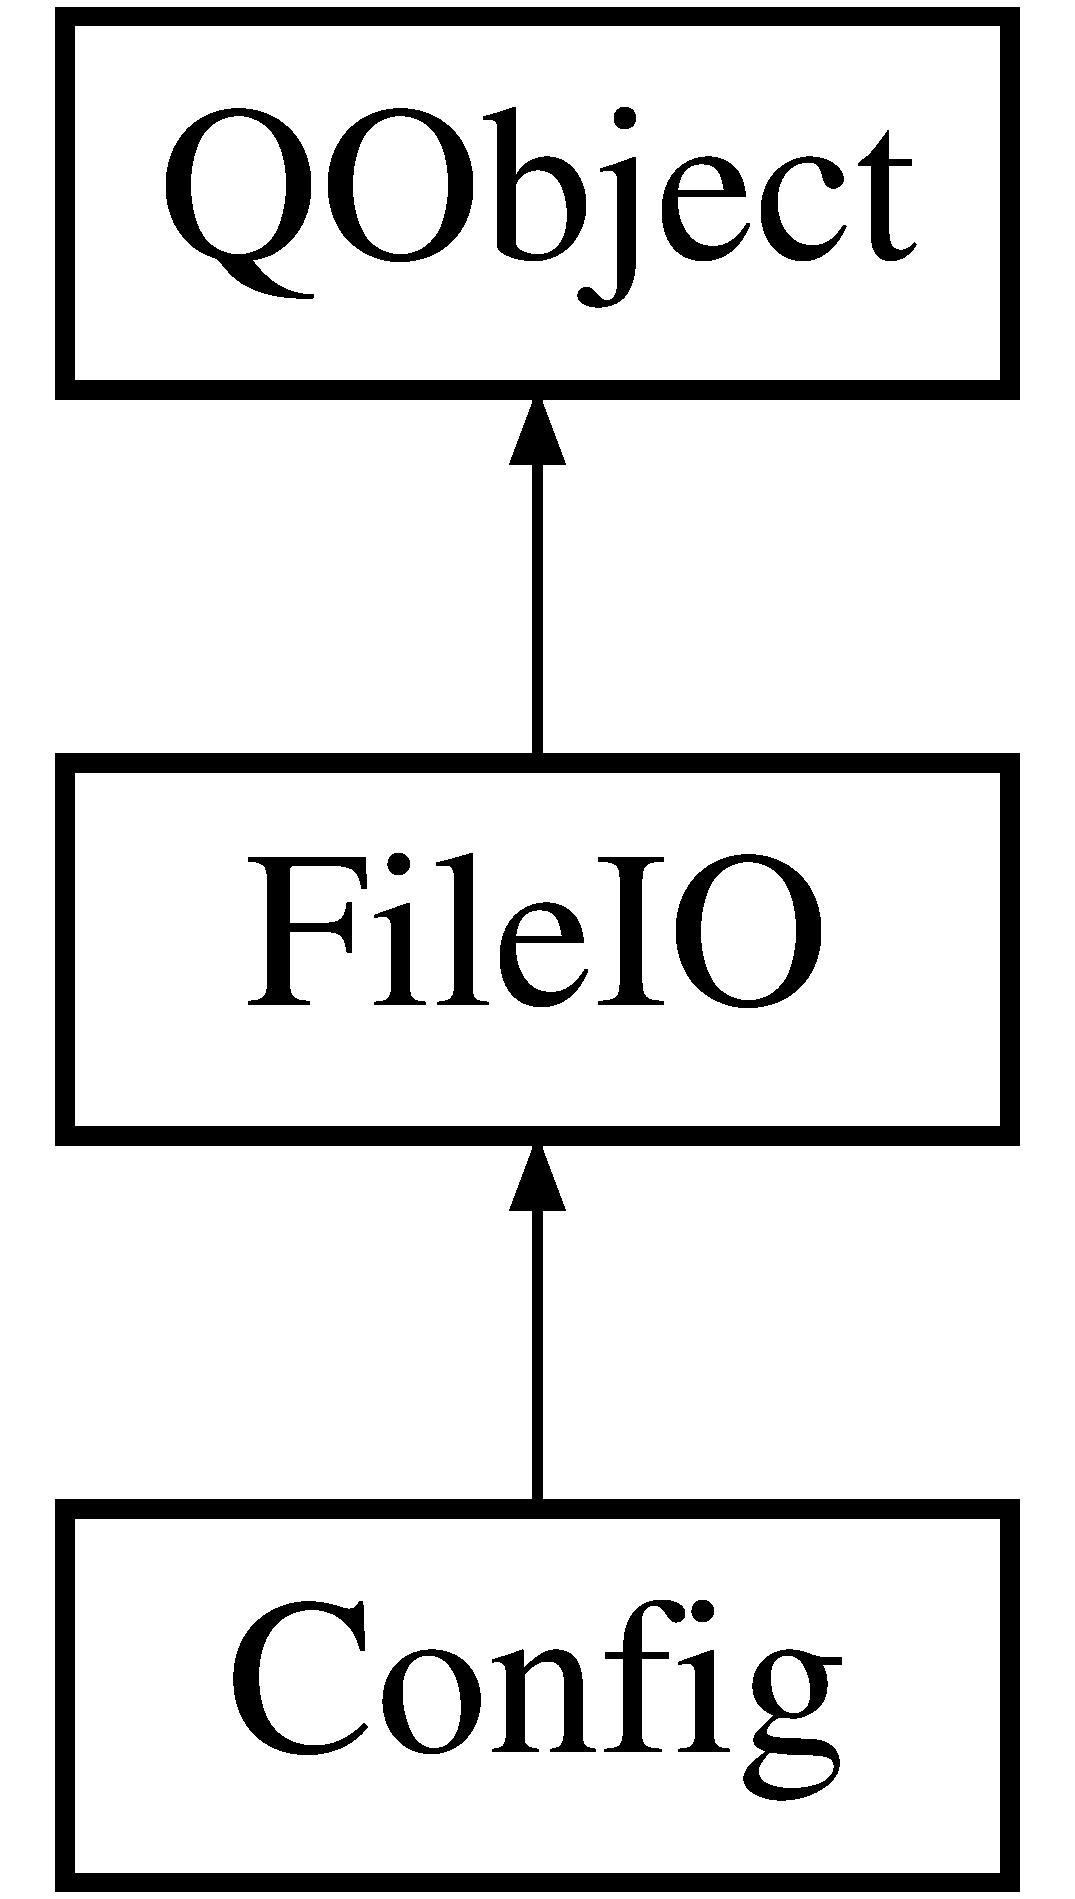
\includegraphics[height=3.000000cm]{class_config}
\end{center}
\end{figure}
\subsection*{Signals}
\begin{DoxyCompactItemize}
\item 
void \hyperlink{class_config_a5681c5b14ccda37c70498b984bd706ff}{axis\+Range\+Changed} ()
\item 
void \hyperlink{class_config_a46f1b9a172d4f44882d784e6f880480e}{env\+Map\+Changed} ()
\item 
void \hyperlink{class_config_a4ef0417dbecefc3febeee33cdf93488d}{max\+Gem\+Size\+Changed} ()
\item 
void \hyperlink{class_config_a3d78af7f9a04ae58883f7f309d0f43d7}{min\+Gem\+Size\+Changed} ()
\end{DoxyCompactItemize}
\subsection*{Public Member Functions}
\begin{DoxyCompactItemize}
\item 
virtual \hyperlink{class_config_a543dce59b66475c5108088ee4ce1cdfc}{$\sim$\+Config} ()
\item 
int \hyperlink{class_config_a17e5e932c588503e186f40c2bcff3149}{axis\+Range} ()
\begin{DoxyCompactList}\small\item\em The axis\+Range describes how far the scene expands along all axis. \end{DoxyCompactList}\item 
Q\+String \hyperlink{class_config_ada50183c56178ba20a6d91193901434e}{env\+Map} () const 
\begin{DoxyCompactList}\small\item\em env\+Map is the name of our current environment. The name is the prefix of our environment texture names. \end{DoxyCompactList}\item 
float \hyperlink{class_config_a55adaaba8e9105c2047f485fc1ff737e}{max\+Gem\+Size} () const 
\begin{DoxyCompactList}\small\item\em max\+Gem\+Size is the maximum size a gem could be.  This is the same as maximum scale factor for a gem, because all gems are in range between \mbox{[}-\/1;1\mbox{]} by default. \end{DoxyCompactList}\item 
float \hyperlink{class_config_af5183a4e104ff4d86f112359199a861f}{min\+Gem\+Size} () const 
\begin{DoxyCompactList}\small\item\em min\+Gem\+Size is the minimum size a gem could be.  This is the same as minimum scale factor for a gem, because all gems are in range between \mbox{[}-\/1;1\mbox{]} by default. \end{DoxyCompactList}\item 
void \hyperlink{class_config_ab6e130f2988e1ee72e81e853865708ba}{set\+Axis\+Range} (int \&axis\+Range)
\begin{DoxyCompactList}\small\item\em Sets value of \hyperlink{class_config_a17e5e932c588503e186f40c2bcff3149}{axis\+Range()};. \end{DoxyCompactList}\item 
void \hyperlink{class_config_a5fd3388c946f7ce1ee6342d6c6b15950}{set\+Env\+Map} (const Q\+String \&env\+Map)
\begin{DoxyCompactList}\small\item\em Sets value of env\+Map();. \end{DoxyCompactList}\item 
void \hyperlink{class_config_a4b35695819904d22fc6e01ee3950a4b2}{set\+Max\+Gem\+Size} (float max\+Gem\+Size)
\begin{DoxyCompactList}\small\item\em Sets value of max\+Gem\+Size();. \end{DoxyCompactList}\item 
void \hyperlink{class_config_a7fa7e53435ece969074029efd14e70e2}{set\+Min\+Gem\+Size} (float min\+Gem\+Size)
\begin{DoxyCompactList}\small\item\em Sets value of min\+Gem\+Size();. \end{DoxyCompactList}\end{DoxyCompactItemize}
\subsection*{Static Public Member Functions}
\begin{DoxyCompactItemize}
\item 
static void \hyperlink{class_config_af99cd0f14331b3df3ed82902728c002c}{drop} ()
\begin{DoxyCompactList}\small\item\em Drops current instance of our \hyperlink{class_config}{Config}. \end{DoxyCompactList}\item 
static \hyperlink{class_config}{Config} $\ast$ \hyperlink{class_config_abf1d4539011ef83cac0fef2ac864a3a9}{instance} ()
\begin{DoxyCompactList}\small\item\em The instance of our \hyperlink{class_config}{Config}. \end{DoxyCompactList}\end{DoxyCompactItemize}
\subsection*{Protected Member Functions}
\begin{DoxyCompactItemize}
\item 
\hyperlink{class_config_abd0c571c116924871e30444b192b792a}{Config} ()
\end{DoxyCompactItemize}
\subsection*{Protected Attributes}
\begin{DoxyCompactItemize}
\item 
int \hyperlink{class_config_a5f172b706977841fdcb91351eeae817e}{m\+\_\+axis\+Range}
\item 
Q\+String \hyperlink{class_config_a70804accd579749b776f9c0c3e5c000b}{m\+\_\+env\+Map}
\item 
float \hyperlink{class_config_ae8a0c3906a4d18952a7fbb00868c963e}{m\+\_\+max\+Gem\+Size}
\item 
float \hyperlink{class_config_a7284f245054875419777e7cbad67183c}{m\+\_\+min\+Gem\+Size}
\end{DoxyCompactItemize}
\subsection*{Static Protected Attributes}
\begin{DoxyCompactItemize}
\item 
static \hyperlink{class_config}{Config} $\ast$ \hyperlink{class_config_af8e6282b4a10e5bce08419395394581b}{m\+\_\+instance} = 0
\end{DoxyCompactItemize}


\subsection{Detailed Description}
The \hyperlink{class_config}{Config} class provides easy access to values read out of our config.\+json provided by Config\+View.\+qml.  The config class is implemented as singleton, because these values are used in many various situations. This class works together Config\+View.\+qml. 

\subsection{Constructor \& Destructor Documentation}
\hypertarget{class_config_a543dce59b66475c5108088ee4ce1cdfc}{\index{Config@{Config}!````~Config@{$\sim$\+Config}}
\index{````~Config@{$\sim$\+Config}!Config@{Config}}
\subsubsection[{$\sim$\+Config}]{\setlength{\rightskip}{0pt plus 5cm}Config\+::$\sim$\+Config (
\begin{DoxyParamCaption}
{}
\end{DoxyParamCaption}
)\hspace{0.3cm}{\ttfamily [virtual]}}}\label{class_config_a543dce59b66475c5108088ee4ce1cdfc}
\hypertarget{class_config_abd0c571c116924871e30444b192b792a}{\index{Config@{Config}!Config@{Config}}
\index{Config@{Config}!Config@{Config}}
\subsubsection[{Config}]{\setlength{\rightskip}{0pt plus 5cm}Config\+::\+Config (
\begin{DoxyParamCaption}
{}
\end{DoxyParamCaption}
)\hspace{0.3cm}{\ttfamily [protected]}}}\label{class_config_abd0c571c116924871e30444b192b792a}


\subsection{Member Function Documentation}
\hypertarget{class_config_a17e5e932c588503e186f40c2bcff3149}{\index{Config@{Config}!axis\+Range@{axis\+Range}}
\index{axis\+Range@{axis\+Range}!Config@{Config}}
\subsubsection[{axis\+Range}]{\setlength{\rightskip}{0pt plus 5cm}int Config\+::axis\+Range (
\begin{DoxyParamCaption}
{}
\end{DoxyParamCaption}
)}}\label{class_config_a17e5e932c588503e186f40c2bcff3149}


The axis\+Range describes how far the scene expands along all axis. 

\begin{DoxyReturn}{Returns}
The value of axis\+Range 
\end{DoxyReturn}
\begin{DoxySeeAlso}{See also}
\hyperlink{class_config_ab6e130f2988e1ee72e81e853865708ba}{set\+Axis\+Range()} 
\end{DoxySeeAlso}
\hypertarget{class_config_a5681c5b14ccda37c70498b984bd706ff}{\index{Config@{Config}!axis\+Range\+Changed@{axis\+Range\+Changed}}
\index{axis\+Range\+Changed@{axis\+Range\+Changed}!Config@{Config}}
\subsubsection[{axis\+Range\+Changed}]{\setlength{\rightskip}{0pt plus 5cm}void Config\+::axis\+Range\+Changed (
\begin{DoxyParamCaption}
{}
\end{DoxyParamCaption}
)\hspace{0.3cm}{\ttfamily [signal]}}}\label{class_config_a5681c5b14ccda37c70498b984bd706ff}
\hypertarget{class_config_af99cd0f14331b3df3ed82902728c002c}{\index{Config@{Config}!drop@{drop}}
\index{drop@{drop}!Config@{Config}}
\subsubsection[{drop}]{\setlength{\rightskip}{0pt plus 5cm}void Config\+::drop (
\begin{DoxyParamCaption}
{}
\end{DoxyParamCaption}
)\hspace{0.3cm}{\ttfamily [static]}}}\label{class_config_af99cd0f14331b3df3ed82902728c002c}


Drops current instance of our \hyperlink{class_config}{Config}. 

\hypertarget{class_config_ada50183c56178ba20a6d91193901434e}{\index{Config@{Config}!env\+Map@{env\+Map}}
\index{env\+Map@{env\+Map}!Config@{Config}}
\subsubsection[{env\+Map}]{\setlength{\rightskip}{0pt plus 5cm}Q\+String Config\+::env\+Map (
\begin{DoxyParamCaption}
{}
\end{DoxyParamCaption}
) const}}\label{class_config_ada50183c56178ba20a6d91193901434e}


env\+Map is the name of our current environment. The name is the prefix of our environment texture names. 

\begin{DoxyReturn}{Returns}

\end{DoxyReturn}
\hypertarget{class_config_a46f1b9a172d4f44882d784e6f880480e}{\index{Config@{Config}!env\+Map\+Changed@{env\+Map\+Changed}}
\index{env\+Map\+Changed@{env\+Map\+Changed}!Config@{Config}}
\subsubsection[{env\+Map\+Changed}]{\setlength{\rightskip}{0pt plus 5cm}void Config\+::env\+Map\+Changed (
\begin{DoxyParamCaption}
{}
\end{DoxyParamCaption}
)\hspace{0.3cm}{\ttfamily [signal]}}}\label{class_config_a46f1b9a172d4f44882d784e6f880480e}
\hypertarget{class_config_abf1d4539011ef83cac0fef2ac864a3a9}{\index{Config@{Config}!instance@{instance}}
\index{instance@{instance}!Config@{Config}}
\subsubsection[{instance}]{\setlength{\rightskip}{0pt plus 5cm}{\bf Config} $\ast$ Config\+::instance (
\begin{DoxyParamCaption}
{}
\end{DoxyParamCaption}
)\hspace{0.3cm}{\ttfamily [static]}}}\label{class_config_abf1d4539011ef83cac0fef2ac864a3a9}


The instance of our \hyperlink{class_config}{Config}. 

\begin{DoxyReturn}{Returns}

\end{DoxyReturn}
\hypertarget{class_config_a55adaaba8e9105c2047f485fc1ff737e}{\index{Config@{Config}!max\+Gem\+Size@{max\+Gem\+Size}}
\index{max\+Gem\+Size@{max\+Gem\+Size}!Config@{Config}}
\subsubsection[{max\+Gem\+Size}]{\setlength{\rightskip}{0pt plus 5cm}float Config\+::max\+Gem\+Size (
\begin{DoxyParamCaption}
{}
\end{DoxyParamCaption}
) const}}\label{class_config_a55adaaba8e9105c2047f485fc1ff737e}


max\+Gem\+Size is the maximum size a gem could be.  This is the same as maximum scale factor for a gem, because all gems are in range between \mbox{[}-\/1;1\mbox{]} by default. 

\begin{DoxyReturn}{Returns}

\end{DoxyReturn}
\begin{DoxySeeAlso}{See also}
\hyperlink{class_config_a4b35695819904d22fc6e01ee3950a4b2}{set\+Max\+Gem\+Size()} 
\end{DoxySeeAlso}
\hypertarget{class_config_a4ef0417dbecefc3febeee33cdf93488d}{\index{Config@{Config}!max\+Gem\+Size\+Changed@{max\+Gem\+Size\+Changed}}
\index{max\+Gem\+Size\+Changed@{max\+Gem\+Size\+Changed}!Config@{Config}}
\subsubsection[{max\+Gem\+Size\+Changed}]{\setlength{\rightskip}{0pt plus 5cm}void Config\+::max\+Gem\+Size\+Changed (
\begin{DoxyParamCaption}
{}
\end{DoxyParamCaption}
)\hspace{0.3cm}{\ttfamily [signal]}}}\label{class_config_a4ef0417dbecefc3febeee33cdf93488d}
\hypertarget{class_config_af5183a4e104ff4d86f112359199a861f}{\index{Config@{Config}!min\+Gem\+Size@{min\+Gem\+Size}}
\index{min\+Gem\+Size@{min\+Gem\+Size}!Config@{Config}}
\subsubsection[{min\+Gem\+Size}]{\setlength{\rightskip}{0pt plus 5cm}float Config\+::min\+Gem\+Size (
\begin{DoxyParamCaption}
{}
\end{DoxyParamCaption}
) const}}\label{class_config_af5183a4e104ff4d86f112359199a861f}


min\+Gem\+Size is the minimum size a gem could be.  This is the same as minimum scale factor for a gem, because all gems are in range between \mbox{[}-\/1;1\mbox{]} by default. 

\begin{DoxyReturn}{Returns}

\end{DoxyReturn}
\hypertarget{class_config_a3d78af7f9a04ae58883f7f309d0f43d7}{\index{Config@{Config}!min\+Gem\+Size\+Changed@{min\+Gem\+Size\+Changed}}
\index{min\+Gem\+Size\+Changed@{min\+Gem\+Size\+Changed}!Config@{Config}}
\subsubsection[{min\+Gem\+Size\+Changed}]{\setlength{\rightskip}{0pt plus 5cm}void Config\+::min\+Gem\+Size\+Changed (
\begin{DoxyParamCaption}
{}
\end{DoxyParamCaption}
)\hspace{0.3cm}{\ttfamily [signal]}}}\label{class_config_a3d78af7f9a04ae58883f7f309d0f43d7}
\hypertarget{class_config_ab6e130f2988e1ee72e81e853865708ba}{\index{Config@{Config}!set\+Axis\+Range@{set\+Axis\+Range}}
\index{set\+Axis\+Range@{set\+Axis\+Range}!Config@{Config}}
\subsubsection[{set\+Axis\+Range}]{\setlength{\rightskip}{0pt plus 5cm}void Config\+::set\+Axis\+Range (
\begin{DoxyParamCaption}
\item[{int \&}]{axis\+Range}
\end{DoxyParamCaption}
)}}\label{class_config_ab6e130f2988e1ee72e81e853865708ba}


Sets value of \hyperlink{class_config_a17e5e932c588503e186f40c2bcff3149}{axis\+Range()};. 


\begin{DoxyParams}{Parameters}
{\em The} & new value \\
\hline
\end{DoxyParams}
\hypertarget{class_config_a5fd3388c946f7ce1ee6342d6c6b15950}{\index{Config@{Config}!set\+Env\+Map@{set\+Env\+Map}}
\index{set\+Env\+Map@{set\+Env\+Map}!Config@{Config}}
\subsubsection[{set\+Env\+Map}]{\setlength{\rightskip}{0pt plus 5cm}void Config\+::set\+Env\+Map (
\begin{DoxyParamCaption}
\item[{const Q\+String \&}]{env\+Map}
\end{DoxyParamCaption}
)}}\label{class_config_a5fd3388c946f7ce1ee6342d6c6b15950}


Sets value of env\+Map();. 


\begin{DoxyParams}{Parameters}
{\em The} & new value \\
\hline
\end{DoxyParams}
\hypertarget{class_config_a4b35695819904d22fc6e01ee3950a4b2}{\index{Config@{Config}!set\+Max\+Gem\+Size@{set\+Max\+Gem\+Size}}
\index{set\+Max\+Gem\+Size@{set\+Max\+Gem\+Size}!Config@{Config}}
\subsubsection[{set\+Max\+Gem\+Size}]{\setlength{\rightskip}{0pt plus 5cm}void Config\+::set\+Max\+Gem\+Size (
\begin{DoxyParamCaption}
\item[{float}]{max\+Gem\+Size}
\end{DoxyParamCaption}
)}}\label{class_config_a4b35695819904d22fc6e01ee3950a4b2}


Sets value of max\+Gem\+Size();. 


\begin{DoxyParams}{Parameters}
{\em The} & new value \\
\hline
\end{DoxyParams}
\hypertarget{class_config_a7fa7e53435ece969074029efd14e70e2}{\index{Config@{Config}!set\+Min\+Gem\+Size@{set\+Min\+Gem\+Size}}
\index{set\+Min\+Gem\+Size@{set\+Min\+Gem\+Size}!Config@{Config}}
\subsubsection[{set\+Min\+Gem\+Size}]{\setlength{\rightskip}{0pt plus 5cm}void Config\+::set\+Min\+Gem\+Size (
\begin{DoxyParamCaption}
\item[{float}]{min\+Gem\+Size}
\end{DoxyParamCaption}
)}}\label{class_config_a7fa7e53435ece969074029efd14e70e2}


Sets value of min\+Gem\+Size();. 


\begin{DoxyParams}{Parameters}
{\em The} & new value \\
\hline
\end{DoxyParams}


\subsection{Member Data Documentation}
\hypertarget{class_config_a5f172b706977841fdcb91351eeae817e}{\index{Config@{Config}!m\+\_\+axis\+Range@{m\+\_\+axis\+Range}}
\index{m\+\_\+axis\+Range@{m\+\_\+axis\+Range}!Config@{Config}}
\subsubsection[{m\+\_\+axis\+Range}]{\setlength{\rightskip}{0pt plus 5cm}int Config\+::m\+\_\+axis\+Range\hspace{0.3cm}{\ttfamily [protected]}}}\label{class_config_a5f172b706977841fdcb91351eeae817e}
\hypertarget{class_config_a70804accd579749b776f9c0c3e5c000b}{\index{Config@{Config}!m\+\_\+env\+Map@{m\+\_\+env\+Map}}
\index{m\+\_\+env\+Map@{m\+\_\+env\+Map}!Config@{Config}}
\subsubsection[{m\+\_\+env\+Map}]{\setlength{\rightskip}{0pt plus 5cm}Q\+String Config\+::m\+\_\+env\+Map\hspace{0.3cm}{\ttfamily [protected]}}}\label{class_config_a70804accd579749b776f9c0c3e5c000b}
\hypertarget{class_config_af8e6282b4a10e5bce08419395394581b}{\index{Config@{Config}!m\+\_\+instance@{m\+\_\+instance}}
\index{m\+\_\+instance@{m\+\_\+instance}!Config@{Config}}
\subsubsection[{m\+\_\+instance}]{\setlength{\rightskip}{0pt plus 5cm}{\bf Config} $\ast$ Config\+::m\+\_\+instance = 0\hspace{0.3cm}{\ttfamily [static]}, {\ttfamily [protected]}}}\label{class_config_af8e6282b4a10e5bce08419395394581b}
\hypertarget{class_config_ae8a0c3906a4d18952a7fbb00868c963e}{\index{Config@{Config}!m\+\_\+max\+Gem\+Size@{m\+\_\+max\+Gem\+Size}}
\index{m\+\_\+max\+Gem\+Size@{m\+\_\+max\+Gem\+Size}!Config@{Config}}
\subsubsection[{m\+\_\+max\+Gem\+Size}]{\setlength{\rightskip}{0pt plus 5cm}float Config\+::m\+\_\+max\+Gem\+Size\hspace{0.3cm}{\ttfamily [protected]}}}\label{class_config_ae8a0c3906a4d18952a7fbb00868c963e}
\hypertarget{class_config_a7284f245054875419777e7cbad67183c}{\index{Config@{Config}!m\+\_\+min\+Gem\+Size@{m\+\_\+min\+Gem\+Size}}
\index{m\+\_\+min\+Gem\+Size@{m\+\_\+min\+Gem\+Size}!Config@{Config}}
\subsubsection[{m\+\_\+min\+Gem\+Size}]{\setlength{\rightskip}{0pt plus 5cm}float Config\+::m\+\_\+min\+Gem\+Size\hspace{0.3cm}{\ttfamily [protected]}}}\label{class_config_a7284f245054875419777e7cbad67183c}


The documentation for this class was generated from the following files\+:\begin{DoxyCompactItemize}
\item 
\hyperlink{config_8h}{config.\+h}\item 
\hyperlink{config_8cpp}{config.\+cpp}\end{DoxyCompactItemize}

\hypertarget{class_cube_gem}{}\section{Cube\+Gem Class Reference}
\label{class_cube_gem}\index{Cube\+Gem@{Cube\+Gem}}


Cube\+Gems are gems with a shape like a cube. The only difference to Abstrac\+Gem is the fact, that a cube gem has a shape defined.  




{\ttfamily \#include $<$cubegem.\+h$>$}

Inheritance diagram for Cube\+Gem\+:\begin{figure}[H]
\begin{center}
\leavevmode
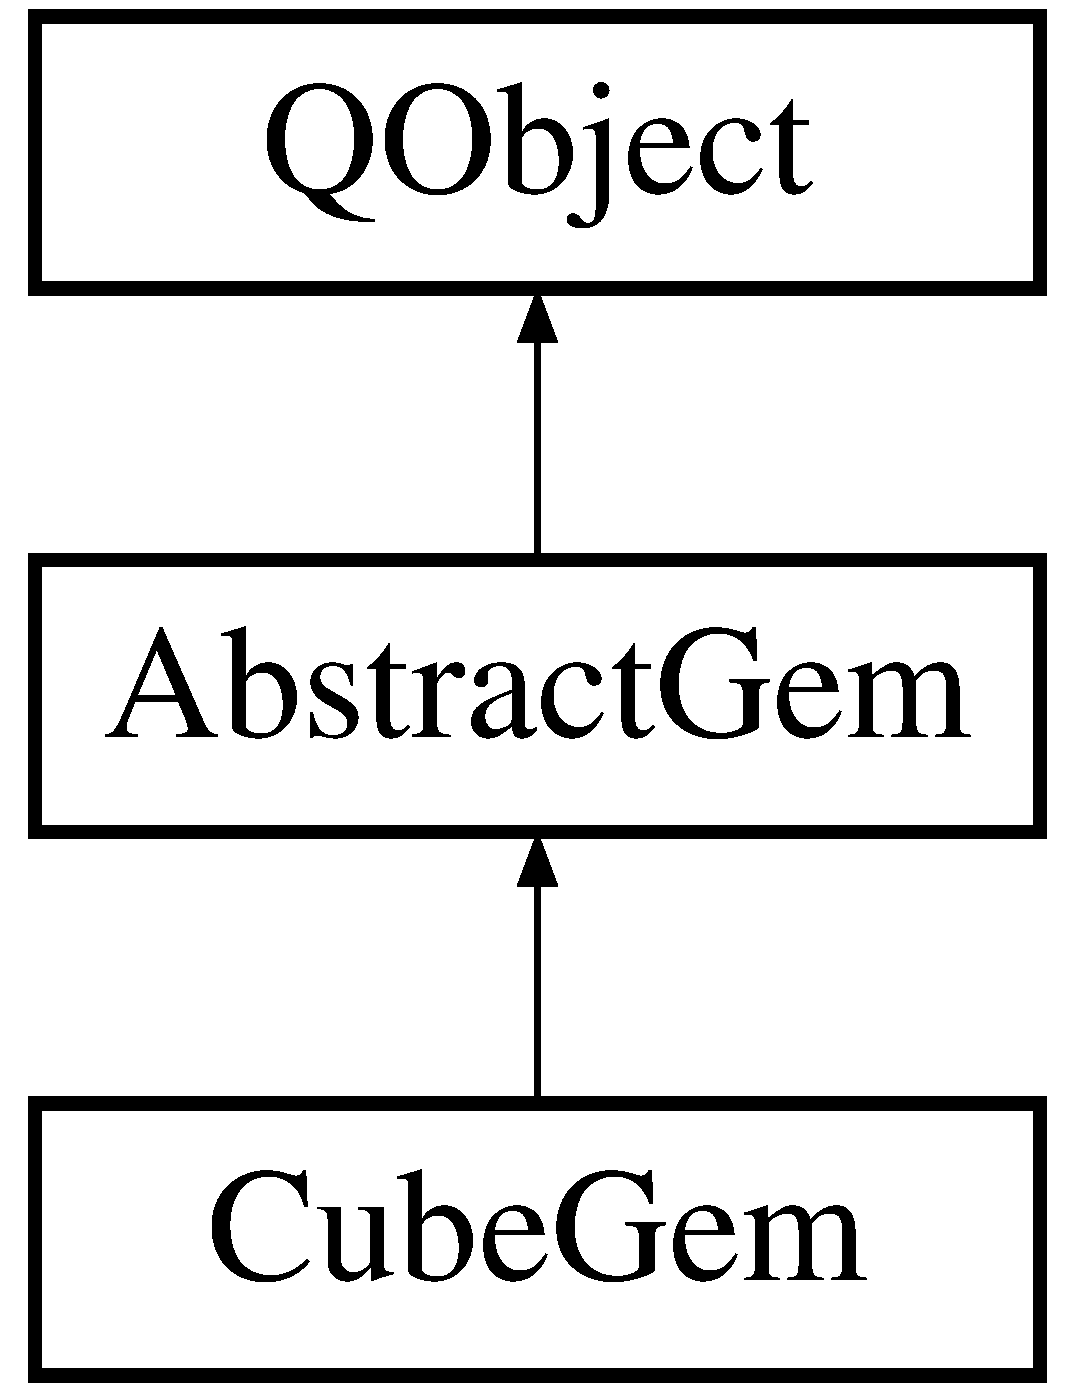
\includegraphics[height=3.000000cm]{class_cube_gem}
\end{center}
\end{figure}
\subsection*{Public Member Functions}
\begin{DoxyCompactItemize}
\item 
\hyperlink{class_cube_gem_a049ed1f21d75e2876cbbc69c56db93c2}{Cube\+Gem} (Q\+Object $\ast$parent=0)
\item 
virtual \hyperlink{class_cube_gem_a6df1dd2ab158e5a0c7bead41d0668140}{$\sim$\+Cube\+Gem} ()
\end{DoxyCompactItemize}
\subsection*{Additional Inherited Members}


\subsection{Detailed Description}
Cube\+Gems are gems with a shape like a cube. The only difference to Abstrac\+Gem is the fact, that a cube gem has a shape defined. 

\subsection{Constructor \& Destructor Documentation}
\hypertarget{class_cube_gem_a049ed1f21d75e2876cbbc69c56db93c2}{}\index{Cube\+Gem@{Cube\+Gem}!Cube\+Gem@{Cube\+Gem}}
\index{Cube\+Gem@{Cube\+Gem}!Cube\+Gem@{Cube\+Gem}}
\subsubsection[{Cube\+Gem}]{\setlength{\rightskip}{0pt plus 5cm}Cube\+Gem\+::\+Cube\+Gem (
\begin{DoxyParamCaption}
\item[{Q\+Object $\ast$}]{parent = {\ttfamily 0}}
\end{DoxyParamCaption}
)\hspace{0.3cm}{\ttfamily [explicit]}}\label{class_cube_gem_a049ed1f21d75e2876cbbc69c56db93c2}
\hypertarget{class_cube_gem_a6df1dd2ab158e5a0c7bead41d0668140}{}\index{Cube\+Gem@{Cube\+Gem}!````~Cube\+Gem@{$\sim$\+Cube\+Gem}}
\index{````~Cube\+Gem@{$\sim$\+Cube\+Gem}!Cube\+Gem@{Cube\+Gem}}
\subsubsection[{$\sim$\+Cube\+Gem}]{\setlength{\rightskip}{0pt plus 5cm}Cube\+Gem\+::$\sim$\+Cube\+Gem (
\begin{DoxyParamCaption}
{}
\end{DoxyParamCaption}
)\hspace{0.3cm}{\ttfamily [virtual]}}\label{class_cube_gem_a6df1dd2ab158e5a0c7bead41d0668140}


The documentation for this class was generated from the following files\+:\begin{DoxyCompactItemize}
\item 
Game-\/\+Programming-\/\+W\+S2014/gem\+Illuminator/\hyperlink{cubegem_8h}{cubegem.\+h}\item 
Game-\/\+Programming-\/\+W\+S2014/gem\+Illuminator/\hyperlink{cubegem_8cpp}{cubegem.\+cpp}\end{DoxyCompactItemize}

\hypertarget{class_cube_map}{\section{Cube\+Map Class Reference}
\label{class_cube_map}\index{Cube\+Map@{Cube\+Map}}
}


The \hyperlink{class_cube_map}{Cube\+Map} class loads cubemap textures and provides them as Open\+G\+L-\/texture.  




{\ttfamily \#include $<$cubemap.\+h$>$}

Inheritance diagram for Cube\+Map\+:\begin{figure}[H]
\begin{center}
\leavevmode
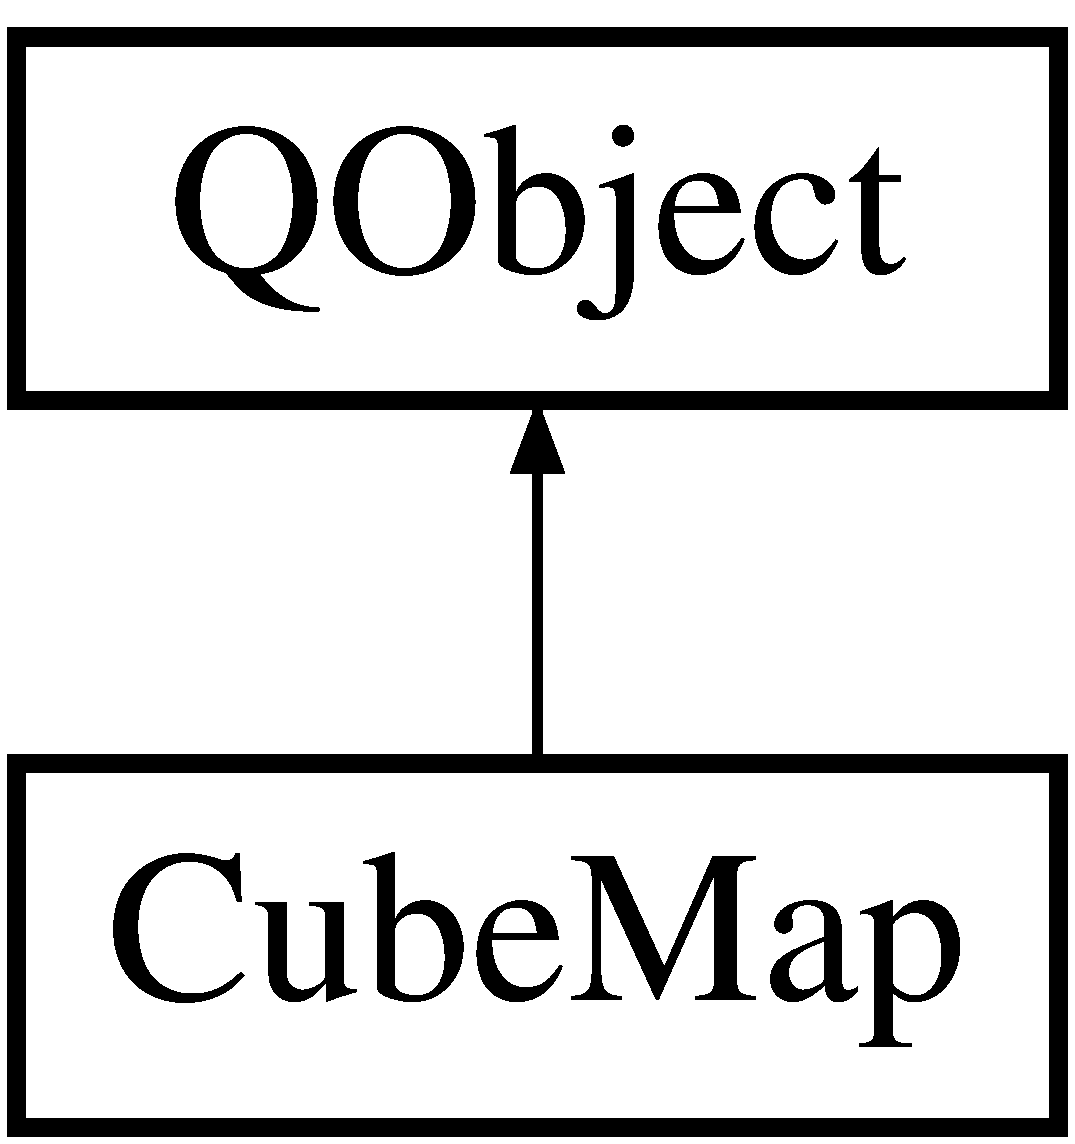
\includegraphics[height=2.000000cm]{class_cube_map}
\end{center}
\end{figure}
\subsection*{Public Member Functions}
\begin{DoxyCompactItemize}
\item 
\hyperlink{class_cube_map_ac1b76abb3b551a933b23f31038855699}{Cube\+Map} (Q\+Open\+G\+L\+Functions \&gl, Q\+String cube\+Map\+Prefix, Q\+Object $\ast$parent=0)
\begin{DoxyCompactList}\small\item\em Creates a new \hyperlink{class_cube_map}{Cube\+Map} and loads required textures. \end{DoxyCompactList}\item 
virtual \hyperlink{class_cube_map_ac4c453248cd7022d3b268755b2dd218e}{$\sim$\+Cube\+Map} ()
\item 
void \hyperlink{class_cube_map_a5d772f8a6b43356593dc909a704354eb}{update} (Q\+String new\+Cube\+Map\+Prefix)
\begin{DoxyCompactList}\small\item\em Replaces current texture with new specified texture. \end{DoxyCompactList}\item 
uint \hyperlink{class_cube_map_a23189c7b896857a6080d1ceb1abf8e4a}{cube\+Map\+Texture} ()
\begin{DoxyCompactList}\small\item\em Open\+G\+L texture reference. \end{DoxyCompactList}\end{DoxyCompactItemize}
\subsection*{Protected Member Functions}
\begin{DoxyCompactItemize}
\item 
void \hyperlink{class_cube_map_a5194b38a4ee4352fe3bdae0c2daf9448}{initialize} ()
\end{DoxyCompactItemize}
\subsection*{Protected Attributes}
\begin{DoxyCompactItemize}
\item 
uint \hyperlink{class_cube_map_a07859b9c39b4c06f4b63e99b00ede4a6}{m\+\_\+cube\+Map}
\item 
Q\+Open\+G\+L\+Functions \& \hyperlink{class_cube_map_aab54def10539c674bd20212eea34a1f0}{m\+\_\+gl}
\item 
Q\+String \hyperlink{class_cube_map_a74ee2f47f59a87bc920c96396a7b33d5}{m\+\_\+cube\+Map\+Prefix}
\end{DoxyCompactItemize}


\subsection{Detailed Description}
The \hyperlink{class_cube_map}{Cube\+Map} class loads cubemap textures and provides them as Open\+G\+L-\/texture. 

\subsection{Constructor \& Destructor Documentation}
\hypertarget{class_cube_map_ac1b76abb3b551a933b23f31038855699}{\index{Cube\+Map@{Cube\+Map}!Cube\+Map@{Cube\+Map}}
\index{Cube\+Map@{Cube\+Map}!Cube\+Map@{Cube\+Map}}
\subsubsection[{Cube\+Map}]{\setlength{\rightskip}{0pt plus 5cm}Cube\+Map\+::\+Cube\+Map (
\begin{DoxyParamCaption}
\item[{Q\+Open\+G\+L\+Functions \&}]{gl, }
\item[{Q\+String}]{cube\+Map\+Prefix, }
\item[{Q\+Object $\ast$}]{parent = {\ttfamily 0}}
\end{DoxyParamCaption}
)}}\label{class_cube_map_ac1b76abb3b551a933b23f31038855699}


Creates a new \hyperlink{class_cube_map}{Cube\+Map} and loads required textures. 


\begin{DoxyParams}{Parameters}
{\em gl} & Q\+Open\+G\+L\+Functions that are used for all gl-\/calls \\
\hline
{\em cube\+Map\+Prefix} & The name of the cubemap. This is the filename of textures without fileextension and face suffix. \\
\hline
{\em parent} & Q\+Object-\/parent \\
\hline
\end{DoxyParams}
\hypertarget{class_cube_map_ac4c453248cd7022d3b268755b2dd218e}{\index{Cube\+Map@{Cube\+Map}!````~Cube\+Map@{$\sim$\+Cube\+Map}}
\index{````~Cube\+Map@{$\sim$\+Cube\+Map}!Cube\+Map@{Cube\+Map}}
\subsubsection[{$\sim$\+Cube\+Map}]{\setlength{\rightskip}{0pt plus 5cm}Cube\+Map\+::$\sim$\+Cube\+Map (
\begin{DoxyParamCaption}
{}
\end{DoxyParamCaption}
)\hspace{0.3cm}{\ttfamily [virtual]}}}\label{class_cube_map_ac4c453248cd7022d3b268755b2dd218e}


\subsection{Member Function Documentation}
\hypertarget{class_cube_map_a23189c7b896857a6080d1ceb1abf8e4a}{\index{Cube\+Map@{Cube\+Map}!cube\+Map\+Texture@{cube\+Map\+Texture}}
\index{cube\+Map\+Texture@{cube\+Map\+Texture}!Cube\+Map@{Cube\+Map}}
\subsubsection[{cube\+Map\+Texture}]{\setlength{\rightskip}{0pt plus 5cm}uint Cube\+Map\+::cube\+Map\+Texture (
\begin{DoxyParamCaption}
{}
\end{DoxyParamCaption}
)}}\label{class_cube_map_a23189c7b896857a6080d1ceb1abf8e4a}


Open\+G\+L texture reference. 

\begin{DoxyReturn}{Returns}

\end{DoxyReturn}
\hypertarget{class_cube_map_a5194b38a4ee4352fe3bdae0c2daf9448}{\index{Cube\+Map@{Cube\+Map}!initialize@{initialize}}
\index{initialize@{initialize}!Cube\+Map@{Cube\+Map}}
\subsubsection[{initialize}]{\setlength{\rightskip}{0pt plus 5cm}void Cube\+Map\+::initialize (
\begin{DoxyParamCaption}
{}
\end{DoxyParamCaption}
)\hspace{0.3cm}{\ttfamily [protected]}}}\label{class_cube_map_a5194b38a4ee4352fe3bdae0c2daf9448}
\hypertarget{class_cube_map_a5d772f8a6b43356593dc909a704354eb}{\index{Cube\+Map@{Cube\+Map}!update@{update}}
\index{update@{update}!Cube\+Map@{Cube\+Map}}
\subsubsection[{update}]{\setlength{\rightskip}{0pt plus 5cm}void Cube\+Map\+::update (
\begin{DoxyParamCaption}
\item[{Q\+String}]{new\+Cube\+Map\+Prefix}
\end{DoxyParamCaption}
)}}\label{class_cube_map_a5d772f8a6b43356593dc909a704354eb}


Replaces current texture with new specified texture. 


\begin{DoxyParams}{Parameters}
{\em new\+Cube\+Map\+Prefix} & The name of the new cubemap. This is the filename of textures without fileextension and face suffix. \\
\hline
\end{DoxyParams}


\subsection{Member Data Documentation}
\hypertarget{class_cube_map_a07859b9c39b4c06f4b63e99b00ede4a6}{\index{Cube\+Map@{Cube\+Map}!m\+\_\+cube\+Map@{m\+\_\+cube\+Map}}
\index{m\+\_\+cube\+Map@{m\+\_\+cube\+Map}!Cube\+Map@{Cube\+Map}}
\subsubsection[{m\+\_\+cube\+Map}]{\setlength{\rightskip}{0pt plus 5cm}uint Cube\+Map\+::m\+\_\+cube\+Map\hspace{0.3cm}{\ttfamily [protected]}}}\label{class_cube_map_a07859b9c39b4c06f4b63e99b00ede4a6}
\hypertarget{class_cube_map_a74ee2f47f59a87bc920c96396a7b33d5}{\index{Cube\+Map@{Cube\+Map}!m\+\_\+cube\+Map\+Prefix@{m\+\_\+cube\+Map\+Prefix}}
\index{m\+\_\+cube\+Map\+Prefix@{m\+\_\+cube\+Map\+Prefix}!Cube\+Map@{Cube\+Map}}
\subsubsection[{m\+\_\+cube\+Map\+Prefix}]{\setlength{\rightskip}{0pt plus 5cm}Q\+String Cube\+Map\+::m\+\_\+cube\+Map\+Prefix\hspace{0.3cm}{\ttfamily [protected]}}}\label{class_cube_map_a74ee2f47f59a87bc920c96396a7b33d5}
\hypertarget{class_cube_map_aab54def10539c674bd20212eea34a1f0}{\index{Cube\+Map@{Cube\+Map}!m\+\_\+gl@{m\+\_\+gl}}
\index{m\+\_\+gl@{m\+\_\+gl}!Cube\+Map@{Cube\+Map}}
\subsubsection[{m\+\_\+gl}]{\setlength{\rightskip}{0pt plus 5cm}Q\+Open\+G\+L\+Functions\& Cube\+Map\+::m\+\_\+gl\hspace{0.3cm}{\ttfamily [protected]}}}\label{class_cube_map_aab54def10539c674bd20212eea34a1f0}


The documentation for this class was generated from the following files\+:\begin{DoxyCompactItemize}
\item 
\hyperlink{cubemap_8h}{cubemap.\+h}\item 
\hyperlink{cubemap_8cpp}{cubemap.\+cpp}\end{DoxyCompactItemize}

\hypertarget{class_environment_map}{\section{Environment\+Map Class Reference}
\label{class_environment_map}\index{Environment\+Map@{Environment\+Map}}
}


The \hyperlink{class_environment_map}{Environment\+Map} is a \hyperlink{class_cube_map}{Cube\+Map} based rendering technique for showing some scene enviroment.  




{\ttfamily \#include $<$environmentmap.\+h$>$}

Inheritance diagram for Environment\+Map\+:\begin{figure}[H]
\begin{center}
\leavevmode
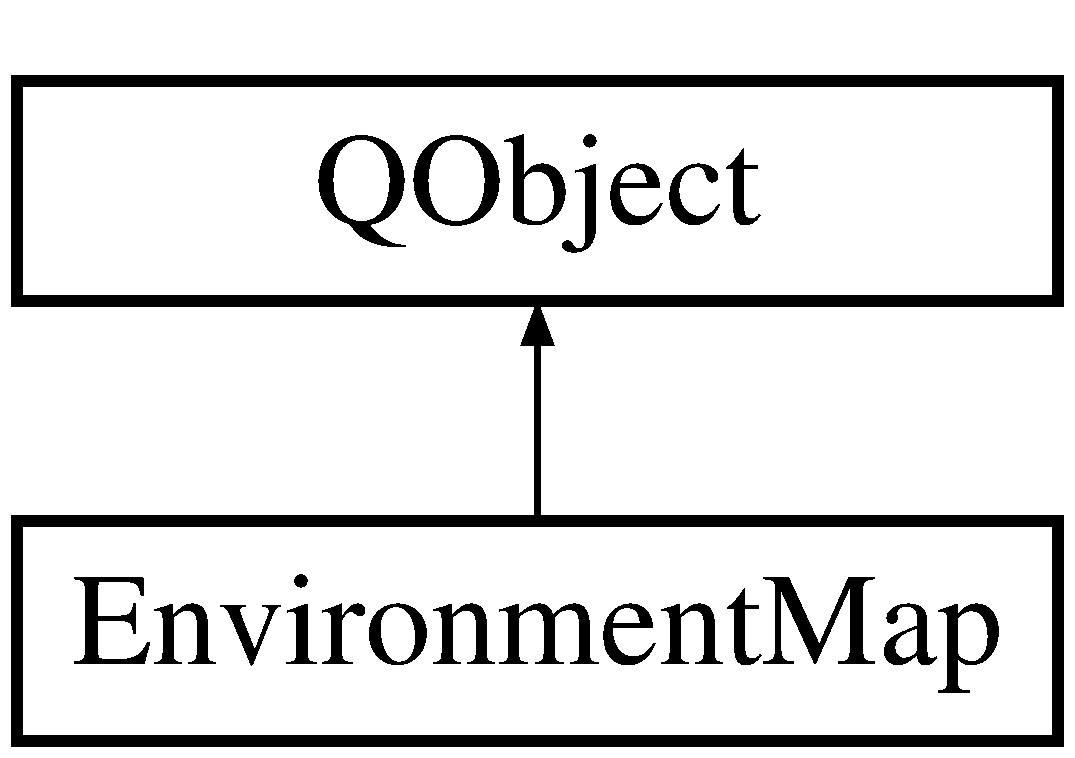
\includegraphics[height=2.000000cm]{class_environment_map}
\end{center}
\end{figure}
\subsection*{Public Member Functions}
\begin{DoxyCompactItemize}
\item 
\hyperlink{class_environment_map_a54b674f88e757c7293abd2f52f518183}{Environment\+Map} (Q\+Open\+G\+L\+Functions \&gl, Q\+String cube\+Map\+Prefix, Q\+Object $\ast$parent=0)
\begin{DoxyCompactList}\small\item\em Creates a new \hyperlink{class_environment_map}{Environment\+Map}. The specified cube map textures are loaded immediately. \end{DoxyCompactList}\item 
\hyperlink{class_environment_map_a77218340957b486754db0ff73f37c8da}{$\sim$\+Environment\+Map} ()
\item 
void \hyperlink{class_environment_map_a49b3996bb58c2e39befdea946402bbdd}{paint} (const \hyperlink{class_camera}{Camera} \&camera)
\begin{DoxyCompactList}\small\item\em Paints environmentmap into the scene using a \hyperlink{class_screen_aligned_quad}{Screen\+Aligned\+Quad}. \end{DoxyCompactList}\item 
void \hyperlink{class_environment_map_a700a5d20db46b88e2ad09675cfeb5a7f}{update} (Q\+String new\+Cube\+Map\+Prefix)
\begin{DoxyCompactList}\small\item\em Replace current \hyperlink{class_cube_map}{Cube\+Map} with new one specified by name. \end{DoxyCompactList}\item 
uint \hyperlink{class_environment_map_a49de5c6028aaf39124e6f6177aeff3db}{cube\+Map\+Texture} ()
\begin{DoxyCompactList}\small\item\em Open\+G\+L texture that is used for drawing. \end{DoxyCompactList}\end{DoxyCompactItemize}
\subsection*{Protected Member Functions}
\begin{DoxyCompactItemize}
\item 
void \hyperlink{class_environment_map_a718a9c79e383200989d22a580520fe80}{initialize} ()
\item 
void \hyperlink{class_environment_map_af348237ba84d4ac5ca45448b4a605357}{initialize\+Shader\+Program} ()
\end{DoxyCompactItemize}
\subsection*{Protected Attributes}
\begin{DoxyCompactItemize}
\item 
\hyperlink{class_cube_map}{Cube\+Map} $\ast$ \hyperlink{class_environment_map_a71fa459b1a6a88e3590cd38109bfc912}{m\+\_\+cube\+Map}
\item 
bool \hyperlink{class_environment_map_af40184d2ae6b58e909fd3c6bf1c32284}{m\+\_\+initialized}
\item 
Q\+Open\+G\+L\+Functions \& \hyperlink{class_environment_map_ad55c368a6c119293a62818a89c80da0a}{m\+\_\+gl}
\item 
\hyperlink{class_screen_aligned_quad}{Screen\+Aligned\+Quad} $\ast$ \hyperlink{class_environment_map_a2d4e6cabcbc17b659bf6dbc68069767c}{m\+\_\+quad}
\item 
Q\+Open\+G\+L\+Shader\+Program $\ast$ \hyperlink{class_environment_map_aab51ee095ecbe9fcaab64d5c8d3b3ab3}{m\+\_\+shader\+Program}
\end{DoxyCompactItemize}


\subsection{Detailed Description}
The \hyperlink{class_environment_map}{Environment\+Map} is a \hyperlink{class_cube_map}{Cube\+Map} based rendering technique for showing some scene enviroment. 

\subsection{Constructor \& Destructor Documentation}
\hypertarget{class_environment_map_a54b674f88e757c7293abd2f52f518183}{\index{Environment\+Map@{Environment\+Map}!Environment\+Map@{Environment\+Map}}
\index{Environment\+Map@{Environment\+Map}!Environment\+Map@{Environment\+Map}}
\subsubsection[{Environment\+Map}]{\setlength{\rightskip}{0pt plus 5cm}Environment\+Map\+::\+Environment\+Map (
\begin{DoxyParamCaption}
\item[{Q\+Open\+G\+L\+Functions \&}]{gl, }
\item[{Q\+String}]{cube\+Map\+Prefix, }
\item[{Q\+Object $\ast$}]{parent = {\ttfamily 0}}
\end{DoxyParamCaption}
)}}\label{class_environment_map_a54b674f88e757c7293abd2f52f518183}


Creates a new \hyperlink{class_environment_map}{Environment\+Map}. The specified cube map textures are loaded immediately. 


\begin{DoxyParams}{Parameters}
{\em gl} & The Q\+Open\+G\+L\+Functions which are used for every gl-\/call \\
\hline
{\em cube\+Map\+Prefix} & The name of cubemap that should be shown. \\
\hline
{\em parent} & Q\+Object-\/parent \\
\hline
\end{DoxyParams}
\hypertarget{class_environment_map_a77218340957b486754db0ff73f37c8da}{\index{Environment\+Map@{Environment\+Map}!````~Environment\+Map@{$\sim$\+Environment\+Map}}
\index{````~Environment\+Map@{$\sim$\+Environment\+Map}!Environment\+Map@{Environment\+Map}}
\subsubsection[{$\sim$\+Environment\+Map}]{\setlength{\rightskip}{0pt plus 5cm}Environment\+Map\+::$\sim$\+Environment\+Map (
\begin{DoxyParamCaption}
{}
\end{DoxyParamCaption}
)}}\label{class_environment_map_a77218340957b486754db0ff73f37c8da}


\subsection{Member Function Documentation}
\hypertarget{class_environment_map_a49de5c6028aaf39124e6f6177aeff3db}{\index{Environment\+Map@{Environment\+Map}!cube\+Map\+Texture@{cube\+Map\+Texture}}
\index{cube\+Map\+Texture@{cube\+Map\+Texture}!Environment\+Map@{Environment\+Map}}
\subsubsection[{cube\+Map\+Texture}]{\setlength{\rightskip}{0pt plus 5cm}uint Environment\+Map\+::cube\+Map\+Texture (
\begin{DoxyParamCaption}
{}
\end{DoxyParamCaption}
)}}\label{class_environment_map_a49de5c6028aaf39124e6f6177aeff3db}


Open\+G\+L texture that is used for drawing. 

\begin{DoxyReturn}{Returns}

\end{DoxyReturn}
\hypertarget{class_environment_map_a718a9c79e383200989d22a580520fe80}{\index{Environment\+Map@{Environment\+Map}!initialize@{initialize}}
\index{initialize@{initialize}!Environment\+Map@{Environment\+Map}}
\subsubsection[{initialize}]{\setlength{\rightskip}{0pt plus 5cm}void Environment\+Map\+::initialize (
\begin{DoxyParamCaption}
{}
\end{DoxyParamCaption}
)\hspace{0.3cm}{\ttfamily [protected]}}}\label{class_environment_map_a718a9c79e383200989d22a580520fe80}
\hypertarget{class_environment_map_af348237ba84d4ac5ca45448b4a605357}{\index{Environment\+Map@{Environment\+Map}!initialize\+Shader\+Program@{initialize\+Shader\+Program}}
\index{initialize\+Shader\+Program@{initialize\+Shader\+Program}!Environment\+Map@{Environment\+Map}}
\subsubsection[{initialize\+Shader\+Program}]{\setlength{\rightskip}{0pt plus 5cm}void Environment\+Map\+::initialize\+Shader\+Program (
\begin{DoxyParamCaption}
{}
\end{DoxyParamCaption}
)\hspace{0.3cm}{\ttfamily [protected]}}}\label{class_environment_map_af348237ba84d4ac5ca45448b4a605357}
\hypertarget{class_environment_map_a49b3996bb58c2e39befdea946402bbdd}{\index{Environment\+Map@{Environment\+Map}!paint@{paint}}
\index{paint@{paint}!Environment\+Map@{Environment\+Map}}
\subsubsection[{paint}]{\setlength{\rightskip}{0pt plus 5cm}void Environment\+Map\+::paint (
\begin{DoxyParamCaption}
\item[{const {\bf Camera} \&}]{camera}
\end{DoxyParamCaption}
)}}\label{class_environment_map_a49b3996bb58c2e39befdea946402bbdd}


Paints environmentmap into the scene using a \hyperlink{class_screen_aligned_quad}{Screen\+Aligned\+Quad}. 


\begin{DoxyParams}{Parameters}
{\em camera} & The camera which is used to render the scene \\
\hline
\end{DoxyParams}
\hypertarget{class_environment_map_a700a5d20db46b88e2ad09675cfeb5a7f}{\index{Environment\+Map@{Environment\+Map}!update@{update}}
\index{update@{update}!Environment\+Map@{Environment\+Map}}
\subsubsection[{update}]{\setlength{\rightskip}{0pt plus 5cm}void Environment\+Map\+::update (
\begin{DoxyParamCaption}
\item[{Q\+String}]{new\+Cube\+Map\+Prefix}
\end{DoxyParamCaption}
)}}\label{class_environment_map_a700a5d20db46b88e2ad09675cfeb5a7f}


Replace current \hyperlink{class_cube_map}{Cube\+Map} with new one specified by name. 


\begin{DoxyParams}{Parameters}
{\em new\+Cube\+Map\+Prefix} & The name of the \hyperlink{class_cube_map}{Cube\+Map} \\
\hline
\end{DoxyParams}
\begin{DoxySeeAlso}{See also}
\hyperlink{class_cube_map_a5d772f8a6b43356593dc909a704354eb}{Cube\+Map\+::update()} 
\end{DoxySeeAlso}


\subsection{Member Data Documentation}
\hypertarget{class_environment_map_a71fa459b1a6a88e3590cd38109bfc912}{\index{Environment\+Map@{Environment\+Map}!m\+\_\+cube\+Map@{m\+\_\+cube\+Map}}
\index{m\+\_\+cube\+Map@{m\+\_\+cube\+Map}!Environment\+Map@{Environment\+Map}}
\subsubsection[{m\+\_\+cube\+Map}]{\setlength{\rightskip}{0pt plus 5cm}{\bf Cube\+Map}$\ast$ Environment\+Map\+::m\+\_\+cube\+Map\hspace{0.3cm}{\ttfamily [protected]}}}\label{class_environment_map_a71fa459b1a6a88e3590cd38109bfc912}
\hypertarget{class_environment_map_ad55c368a6c119293a62818a89c80da0a}{\index{Environment\+Map@{Environment\+Map}!m\+\_\+gl@{m\+\_\+gl}}
\index{m\+\_\+gl@{m\+\_\+gl}!Environment\+Map@{Environment\+Map}}
\subsubsection[{m\+\_\+gl}]{\setlength{\rightskip}{0pt plus 5cm}Q\+Open\+G\+L\+Functions\& Environment\+Map\+::m\+\_\+gl\hspace{0.3cm}{\ttfamily [protected]}}}\label{class_environment_map_ad55c368a6c119293a62818a89c80da0a}
\hypertarget{class_environment_map_af40184d2ae6b58e909fd3c6bf1c32284}{\index{Environment\+Map@{Environment\+Map}!m\+\_\+initialized@{m\+\_\+initialized}}
\index{m\+\_\+initialized@{m\+\_\+initialized}!Environment\+Map@{Environment\+Map}}
\subsubsection[{m\+\_\+initialized}]{\setlength{\rightskip}{0pt plus 5cm}bool Environment\+Map\+::m\+\_\+initialized\hspace{0.3cm}{\ttfamily [protected]}}}\label{class_environment_map_af40184d2ae6b58e909fd3c6bf1c32284}
\hypertarget{class_environment_map_a2d4e6cabcbc17b659bf6dbc68069767c}{\index{Environment\+Map@{Environment\+Map}!m\+\_\+quad@{m\+\_\+quad}}
\index{m\+\_\+quad@{m\+\_\+quad}!Environment\+Map@{Environment\+Map}}
\subsubsection[{m\+\_\+quad}]{\setlength{\rightskip}{0pt plus 5cm}{\bf Screen\+Aligned\+Quad}$\ast$ Environment\+Map\+::m\+\_\+quad\hspace{0.3cm}{\ttfamily [protected]}}}\label{class_environment_map_a2d4e6cabcbc17b659bf6dbc68069767c}
\hypertarget{class_environment_map_aab51ee095ecbe9fcaab64d5c8d3b3ab3}{\index{Environment\+Map@{Environment\+Map}!m\+\_\+shader\+Program@{m\+\_\+shader\+Program}}
\index{m\+\_\+shader\+Program@{m\+\_\+shader\+Program}!Environment\+Map@{Environment\+Map}}
\subsubsection[{m\+\_\+shader\+Program}]{\setlength{\rightskip}{0pt plus 5cm}Q\+Open\+G\+L\+Shader\+Program$\ast$ Environment\+Map\+::m\+\_\+shader\+Program\hspace{0.3cm}{\ttfamily [protected]}}}\label{class_environment_map_aab51ee095ecbe9fcaab64d5c8d3b3ab3}


The documentation for this class was generated from the following files\+:\begin{DoxyCompactItemize}
\item 
\hyperlink{environmentmap_8h}{environmentmap.\+h}\item 
\hyperlink{environmentmap_8cpp}{environmentmap.\+cpp}\end{DoxyCompactItemize}

\hypertarget{class_file_i_o}{\section{File\+I\+O Class Reference}
\label{class_file_i_o}\index{File\+I\+O@{File\+I\+O}}
}


The \hyperlink{class_file_i_o}{File\+I\+O} class provides platform independent file reading for ressource files used by us.  The file that should be read is specified by name and \hyperlink{class_file_i_o}{File\+I\+O} will load it from platform dependent location.  




{\ttfamily \#include $<$fileio.\+h$>$}

Inheritance diagram for File\+I\+O\+:\begin{figure}[H]
\begin{center}
\leavevmode
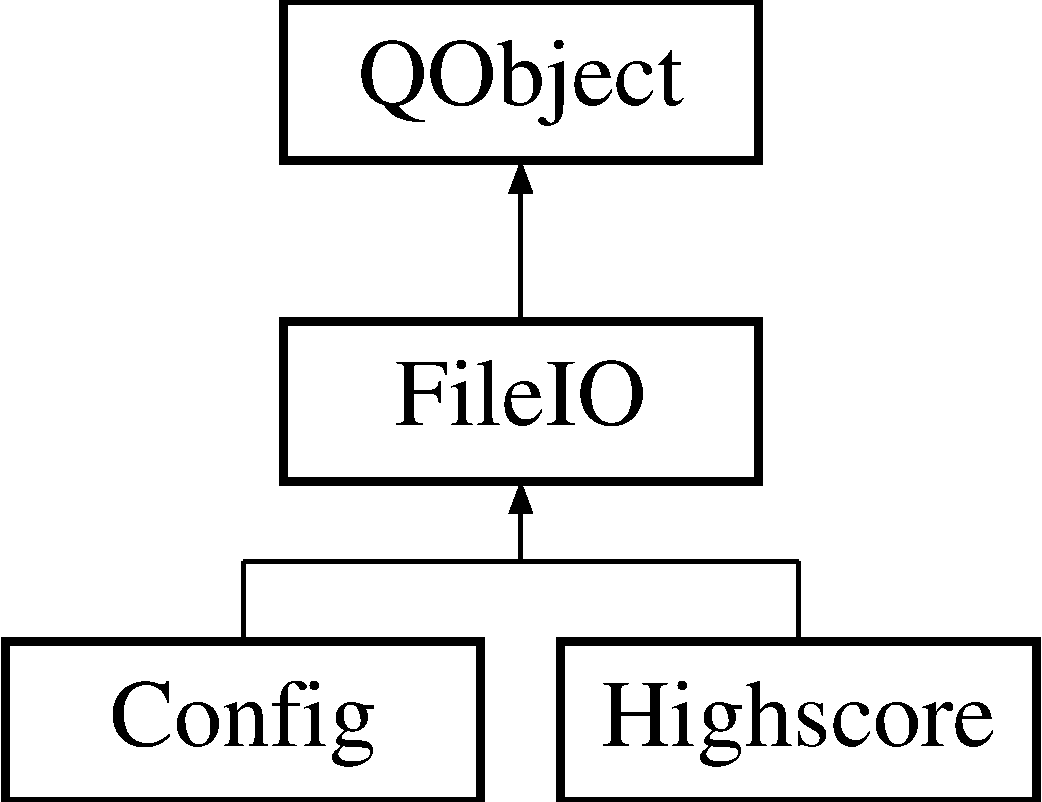
\includegraphics[height=3.000000cm]{class_file_i_o}
\end{center}
\end{figure}
\subsection*{Signals}
\begin{DoxyCompactItemize}
\item 
void \hyperlink{class_file_i_o_a4136bb085d530f9dd54eb849f14d58da}{error} (const Q\+String \&msg)
\begin{DoxyCompactList}\small\item\em This signal will be emitted if an error occurs. \end{DoxyCompactList}\item 
void \hyperlink{class_file_i_o_a31a6e00e907268e4473a0a826d2e6a1e}{source\+Changed} (const Q\+String \&source)
\begin{DoxyCompactList}\small\item\em This signal is emitted if the \hyperlink{class_file_i_o_a8da2b4c6cd72af512e4556203c1c66e7}{source()} is changed. \end{DoxyCompactList}\end{DoxyCompactItemize}
\subsection*{Public Member Functions}
\begin{DoxyCompactItemize}
\item 
\hyperlink{class_file_i_o_a6e4f7122f89b633e3522c2e1d31e1fdd}{File\+I\+O} (Q\+Object $\ast$parent=0)
\begin{DoxyCompactList}\small\item\em Creates a new \hyperlink{class_file_i_o}{File\+I\+O}. \end{DoxyCompactList}\item 
\hyperlink{class_file_i_o_adc3caa8f1e5d76274d8ffb8b5c17288b}{$\sim$\+File\+I\+O} ()
\item 
Q\+\_\+\+I\+N\+V\+O\+K\+A\+B\+L\+E Q\+String \hyperlink{class_file_i_o_a48c90efc3bf8dda4d612f2dff5409834}{read} ()
\begin{DoxyCompactList}\small\item\em Reads previous specified file. \end{DoxyCompactList}\item 
void \hyperlink{class_file_i_o_a985a2cce4d400bca160c5f42bf697adb}{set\+Source} (const Q\+String \&source)
\begin{DoxyCompactList}\small\item\em Sets the source file by name. The source is read calling \hyperlink{class_file_i_o_a48c90efc3bf8dda4d612f2dff5409834}{read()} \end{DoxyCompactList}\item 
Q\+String \hyperlink{class_file_i_o_a8da2b4c6cd72af512e4556203c1c66e7}{source} ()
\begin{DoxyCompactList}\small\item\em The name of file that is read by \hyperlink{class_file_i_o_a48c90efc3bf8dda4d612f2dff5409834}{read()}. \end{DoxyCompactList}\item 
Q\+\_\+\+I\+N\+V\+O\+K\+A\+B\+L\+E bool \hyperlink{class_file_i_o_a73bc6cac958f024325e795a690740a85}{write} (const Q\+String \&data)
\begin{DoxyCompactList}\small\item\em Writes specified data into \hyperlink{class_file_i_o_a8da2b4c6cd72af512e4556203c1c66e7}{source()} \end{DoxyCompactList}\end{DoxyCompactItemize}
\subsection*{Protected Attributes}
\begin{DoxyCompactItemize}
\item 
Q\+String \hyperlink{class_file_i_o_ab8f8edbc97eec6d3cf77e314a8754ef3}{m\+\_\+source}
\end{DoxyCompactItemize}


\subsection{Detailed Description}
The \hyperlink{class_file_i_o}{File\+I\+O} class provides platform independent file reading for ressource files used by us.  The file that should be read is specified by name and \hyperlink{class_file_i_o}{File\+I\+O} will load it from platform dependent location. 

\subsection{Constructor \& Destructor Documentation}
\hypertarget{class_file_i_o_a6e4f7122f89b633e3522c2e1d31e1fdd}{\index{File\+I\+O@{File\+I\+O}!File\+I\+O@{File\+I\+O}}
\index{File\+I\+O@{File\+I\+O}!File\+I\+O@{File\+I\+O}}
\subsubsection[{File\+I\+O}]{\setlength{\rightskip}{0pt plus 5cm}File\+I\+O\+::\+File\+I\+O (
\begin{DoxyParamCaption}
\item[{Q\+Object $\ast$}]{parent = {\ttfamily 0}}
\end{DoxyParamCaption}
)\hspace{0.3cm}{\ttfamily [explicit]}}}\label{class_file_i_o_a6e4f7122f89b633e3522c2e1d31e1fdd}


Creates a new \hyperlink{class_file_i_o}{File\+I\+O}. 


\begin{DoxyParams}{Parameters}
{\em parent} & Q\+Object-\/parent \\
\hline
\end{DoxyParams}
\hypertarget{class_file_i_o_adc3caa8f1e5d76274d8ffb8b5c17288b}{\index{File\+I\+O@{File\+I\+O}!````~File\+I\+O@{$\sim$\+File\+I\+O}}
\index{````~File\+I\+O@{$\sim$\+File\+I\+O}!File\+I\+O@{File\+I\+O}}
\subsubsection[{$\sim$\+File\+I\+O}]{\setlength{\rightskip}{0pt plus 5cm}File\+I\+O\+::$\sim$\+File\+I\+O (
\begin{DoxyParamCaption}
{}
\end{DoxyParamCaption}
)}}\label{class_file_i_o_adc3caa8f1e5d76274d8ffb8b5c17288b}


\subsection{Member Function Documentation}
\hypertarget{class_file_i_o_a4136bb085d530f9dd54eb849f14d58da}{\index{File\+I\+O@{File\+I\+O}!error@{error}}
\index{error@{error}!File\+I\+O@{File\+I\+O}}
\subsubsection[{error}]{\setlength{\rightskip}{0pt plus 5cm}void File\+I\+O\+::error (
\begin{DoxyParamCaption}
\item[{const Q\+String \&}]{msg}
\end{DoxyParamCaption}
)\hspace{0.3cm}{\ttfamily [signal]}}}\label{class_file_i_o_a4136bb085d530f9dd54eb849f14d58da}


This signal will be emitted if an error occurs. 


\begin{DoxyParams}{Parameters}
{\em msg} & The error message describing the error \\
\hline
\end{DoxyParams}
\hypertarget{class_file_i_o_a48c90efc3bf8dda4d612f2dff5409834}{\index{File\+I\+O@{File\+I\+O}!read@{read}}
\index{read@{read}!File\+I\+O@{File\+I\+O}}
\subsubsection[{read}]{\setlength{\rightskip}{0pt plus 5cm}Q\+String File\+I\+O\+::read (
\begin{DoxyParamCaption}
{}
\end{DoxyParamCaption}
)}}\label{class_file_i_o_a48c90efc3bf8dda4d612f2dff5409834}


Reads previous specified file. 

\begin{DoxyReturn}{Returns}
Read file as Q\+String. 
\end{DoxyReturn}
\hypertarget{class_file_i_o_a985a2cce4d400bca160c5f42bf697adb}{\index{File\+I\+O@{File\+I\+O}!set\+Source@{set\+Source}}
\index{set\+Source@{set\+Source}!File\+I\+O@{File\+I\+O}}
\subsubsection[{set\+Source}]{\setlength{\rightskip}{0pt plus 5cm}void File\+I\+O\+::set\+Source (
\begin{DoxyParamCaption}
\item[{const Q\+String \&}]{source}
\end{DoxyParamCaption}
)}}\label{class_file_i_o_a985a2cce4d400bca160c5f42bf697adb}


Sets the source file by name. The source is read calling \hyperlink{class_file_i_o_a48c90efc3bf8dda4d612f2dff5409834}{read()} 


\begin{DoxyParams}{Parameters}
{\em source} & The name of file that should be read. \\
\hline
\end{DoxyParams}
\hypertarget{class_file_i_o_a8da2b4c6cd72af512e4556203c1c66e7}{\index{File\+I\+O@{File\+I\+O}!source@{source}}
\index{source@{source}!File\+I\+O@{File\+I\+O}}
\subsubsection[{source}]{\setlength{\rightskip}{0pt plus 5cm}Q\+String File\+I\+O\+::source (
\begin{DoxyParamCaption}
{}
\end{DoxyParamCaption}
)}}\label{class_file_i_o_a8da2b4c6cd72af512e4556203c1c66e7}


The name of file that is read by \hyperlink{class_file_i_o_a48c90efc3bf8dda4d612f2dff5409834}{read()}. 

\begin{DoxyReturn}{Returns}

\end{DoxyReturn}
\hypertarget{class_file_i_o_a31a6e00e907268e4473a0a826d2e6a1e}{\index{File\+I\+O@{File\+I\+O}!source\+Changed@{source\+Changed}}
\index{source\+Changed@{source\+Changed}!File\+I\+O@{File\+I\+O}}
\subsubsection[{source\+Changed}]{\setlength{\rightskip}{0pt plus 5cm}void File\+I\+O\+::source\+Changed (
\begin{DoxyParamCaption}
\item[{const Q\+String \&}]{source}
\end{DoxyParamCaption}
)\hspace{0.3cm}{\ttfamily [signal]}}}\label{class_file_i_o_a31a6e00e907268e4473a0a826d2e6a1e}


This signal is emitted if the \hyperlink{class_file_i_o_a8da2b4c6cd72af512e4556203c1c66e7}{source()} is changed. 


\begin{DoxyParams}{Parameters}
{\em source} & The new source \\
\hline
\end{DoxyParams}
\hypertarget{class_file_i_o_a73bc6cac958f024325e795a690740a85}{\index{File\+I\+O@{File\+I\+O}!write@{write}}
\index{write@{write}!File\+I\+O@{File\+I\+O}}
\subsubsection[{write}]{\setlength{\rightskip}{0pt plus 5cm}bool File\+I\+O\+::write (
\begin{DoxyParamCaption}
\item[{const Q\+String \&}]{data}
\end{DoxyParamCaption}
)}}\label{class_file_i_o_a73bc6cac958f024325e795a690740a85}


Writes specified data into \hyperlink{class_file_i_o_a8da2b4c6cd72af512e4556203c1c66e7}{source()} 


\begin{DoxyParams}{Parameters}
{\em data} & The data that will be written into \hyperlink{class_file_i_o_a8da2b4c6cd72af512e4556203c1c66e7}{source()} \\
\hline
\end{DoxyParams}


\subsection{Member Data Documentation}
\hypertarget{class_file_i_o_ab8f8edbc97eec6d3cf77e314a8754ef3}{\index{File\+I\+O@{File\+I\+O}!m\+\_\+source@{m\+\_\+source}}
\index{m\+\_\+source@{m\+\_\+source}!File\+I\+O@{File\+I\+O}}
\subsubsection[{m\+\_\+source}]{\setlength{\rightskip}{0pt plus 5cm}Q\+String File\+I\+O\+::m\+\_\+source\hspace{0.3cm}{\ttfamily [protected]}}}\label{class_file_i_o_ab8f8edbc97eec6d3cf77e314a8754ef3}


The documentation for this class was generated from the following files\+:\begin{DoxyCompactItemize}
\item 
\hyperlink{fileio_8h}{fileio.\+h}\item 
\hyperlink{fileio_8cpp}{fileio.\+cpp}\end{DoxyCompactItemize}

\hypertarget{class_game_lost_ray}{}\section{Game\+Lost\+Ray Class Reference}
\label{class_game_lost_ray}\index{Game\+Lost\+Ray@{Game\+Lost\+Ray}}


The \hyperlink{class_game_lost_ray}{Game\+Lost\+Ray} class is a specialized \hyperlink{class_light_ray}{Light\+Ray}, that is created if the player should loose as soon as the player reaches it.  




{\ttfamily \#include $<$gamelostray.\+h$>$}

Inheritance diagram for Game\+Lost\+Ray\+:\begin{figure}[H]
\begin{center}
\leavevmode
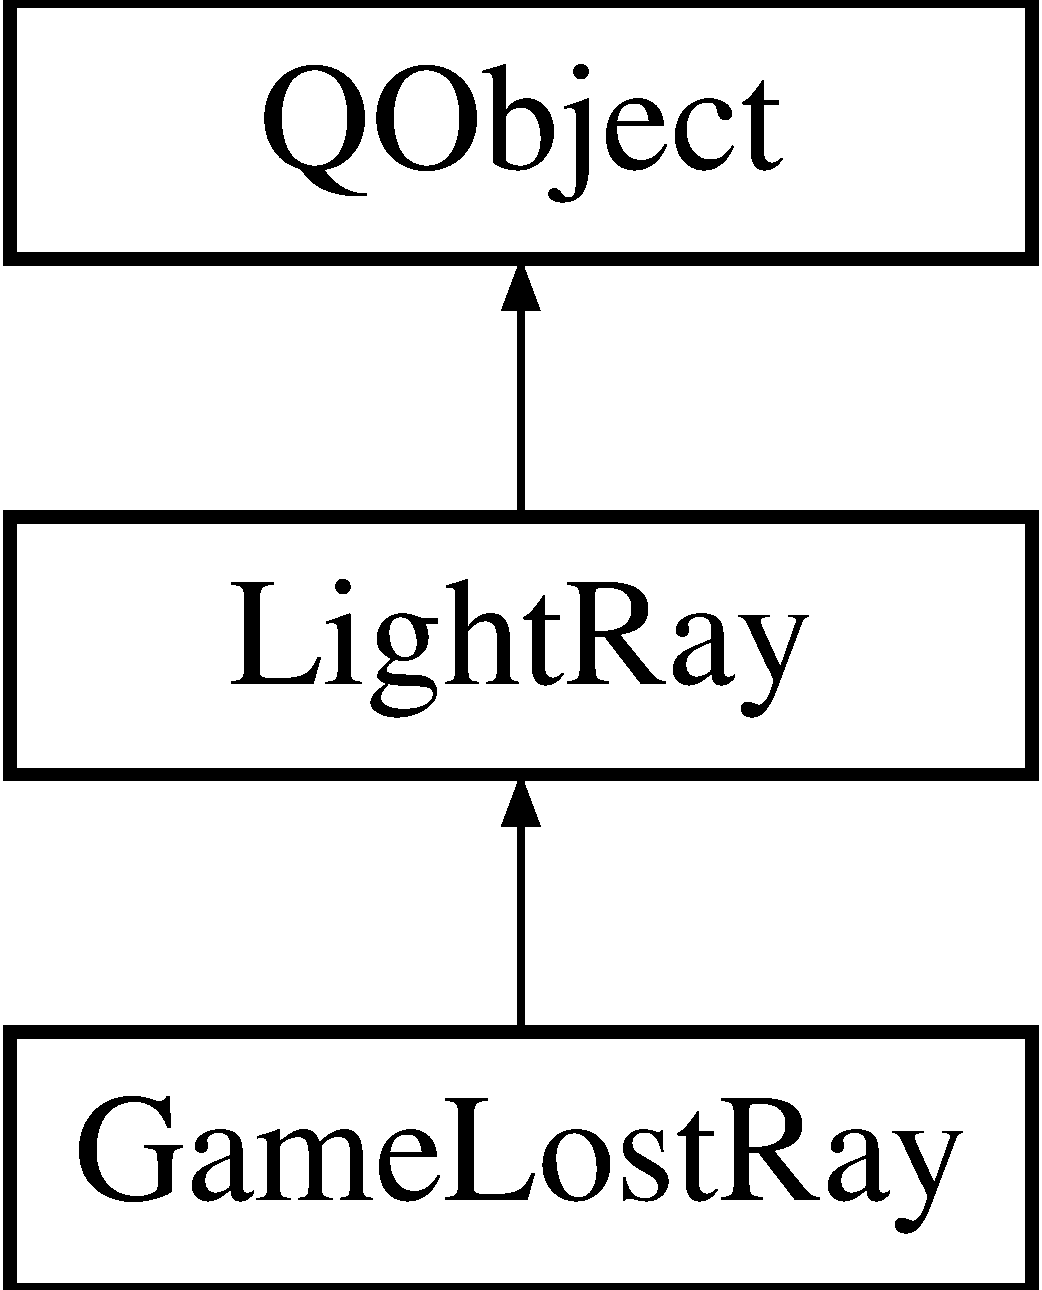
\includegraphics[height=3.000000cm]{class_game_lost_ray}
\end{center}
\end{figure}
\subsection*{Signals}
\begin{DoxyCompactItemize}
\item 
void \hyperlink{class_game_lost_ray_a9b2afbad70387bd9ec8f80170760ef57}{game\+Lost} ()
\begin{DoxyCompactList}\small\item\em The \hyperlink{class_game_lost_ray_a9b2afbad70387bd9ec8f80170760ef57}{game\+Lost()} signal is emitted at that moment the ray detects the player leaving the scene. \end{DoxyCompactList}\end{DoxyCompactItemize}
\subsection*{Public Member Functions}
\begin{DoxyCompactItemize}
\item 
\hyperlink{class_game_lost_ray_a15ec367ee8dfd87bc8deccde5553f8e6}{Game\+Lost\+Ray} (Q\+Object $\ast$parent=0)
\item 
void \hyperlink{class_game_lost_ray_a417d814372891fe7595a7e745b7a9f0f}{update} (int time\+Difference) override
\begin{DoxyCompactList}\small\item\em This method is like \hyperlink{class_light_ray_acf06a71a307433fa5b220baccf809e64}{Light\+Ray\+::update()} with the addition, that the game end is detect a soon as the ray has a player-\/$>$ \end{DoxyCompactList}\end{DoxyCompactItemize}
\subsection*{Protected Attributes}
\begin{DoxyCompactItemize}
\item 
bool \hyperlink{class_game_lost_ray_a9b8fd54b22a3f25d4fef9431cebafa7a}{m\+\_\+already\+Lost}
\end{DoxyCompactItemize}
\subsection*{Additional Inherited Members}


\subsection{Detailed Description}
The \hyperlink{class_game_lost_ray}{Game\+Lost\+Ray} class is a specialized \hyperlink{class_light_ray}{Light\+Ray}, that is created if the player should loose as soon as the player reaches it. 

\subsection{Constructor \& Destructor Documentation}
\hypertarget{class_game_lost_ray_a15ec367ee8dfd87bc8deccde5553f8e6}{}\index{Game\+Lost\+Ray@{Game\+Lost\+Ray}!Game\+Lost\+Ray@{Game\+Lost\+Ray}}
\index{Game\+Lost\+Ray@{Game\+Lost\+Ray}!Game\+Lost\+Ray@{Game\+Lost\+Ray}}
\subsubsection[{Game\+Lost\+Ray}]{\setlength{\rightskip}{0pt plus 5cm}Game\+Lost\+Ray\+::\+Game\+Lost\+Ray (
\begin{DoxyParamCaption}
\item[{Q\+Object $\ast$}]{parent = {\ttfamily 0}}
\end{DoxyParamCaption}
)\hspace{0.3cm}{\ttfamily [explicit]}}\label{class_game_lost_ray_a15ec367ee8dfd87bc8deccde5553f8e6}


\subsection{Member Function Documentation}
\hypertarget{class_game_lost_ray_a9b2afbad70387bd9ec8f80170760ef57}{}\index{Game\+Lost\+Ray@{Game\+Lost\+Ray}!game\+Lost@{game\+Lost}}
\index{game\+Lost@{game\+Lost}!Game\+Lost\+Ray@{Game\+Lost\+Ray}}
\subsubsection[{game\+Lost}]{\setlength{\rightskip}{0pt plus 5cm}void Game\+Lost\+Ray\+::game\+Lost (
\begin{DoxyParamCaption}
{}
\end{DoxyParamCaption}
)\hspace{0.3cm}{\ttfamily [signal]}}\label{class_game_lost_ray_a9b2afbad70387bd9ec8f80170760ef57}


The \hyperlink{class_game_lost_ray_a9b2afbad70387bd9ec8f80170760ef57}{game\+Lost()} signal is emitted at that moment the ray detects the player leaving the scene. 

\hypertarget{class_game_lost_ray_a417d814372891fe7595a7e745b7a9f0f}{}\index{Game\+Lost\+Ray@{Game\+Lost\+Ray}!update@{update}}
\index{update@{update}!Game\+Lost\+Ray@{Game\+Lost\+Ray}}
\subsubsection[{update}]{\setlength{\rightskip}{0pt plus 5cm}void Game\+Lost\+Ray\+::update (
\begin{DoxyParamCaption}
\item[{int}]{time\+Difference}
\end{DoxyParamCaption}
)\hspace{0.3cm}{\ttfamily [override]}, {\ttfamily [virtual]}}\label{class_game_lost_ray_a417d814372891fe7595a7e745b7a9f0f}


This method is like \hyperlink{class_light_ray_acf06a71a307433fa5b220baccf809e64}{Light\+Ray\+::update()} with the addition, that the game end is detect a soon as the ray has a player-\/$>$ 


\begin{DoxyParams}{Parameters}
{\em time\+Difference} & Time differnce to previous update. \\
\hline
\end{DoxyParams}


Reimplemented from \hyperlink{class_light_ray_acf06a71a307433fa5b220baccf809e64}{Light\+Ray}.



\subsection{Member Data Documentation}
\hypertarget{class_game_lost_ray_a9b8fd54b22a3f25d4fef9431cebafa7a}{}\index{Game\+Lost\+Ray@{Game\+Lost\+Ray}!m\+\_\+already\+Lost@{m\+\_\+already\+Lost}}
\index{m\+\_\+already\+Lost@{m\+\_\+already\+Lost}!Game\+Lost\+Ray@{Game\+Lost\+Ray}}
\subsubsection[{m\+\_\+already\+Lost}]{\setlength{\rightskip}{0pt plus 5cm}bool Game\+Lost\+Ray\+::m\+\_\+already\+Lost\hspace{0.3cm}{\ttfamily [protected]}}\label{class_game_lost_ray_a9b8fd54b22a3f25d4fef9431cebafa7a}


The documentation for this class was generated from the following files\+:\begin{DoxyCompactItemize}
\item 
Game-\/\+Programming-\/\+W\+S2014/gem\+Illuminator/\hyperlink{gamelostray_8h}{gamelostray.\+h}\item 
Game-\/\+Programming-\/\+W\+S2014/gem\+Illuminator/\hyperlink{gamelostray_8cpp}{gamelostray.\+cpp}\end{DoxyCompactItemize}

\hypertarget{class_gem_data}{\section{Gem\+Data Class Reference}
\label{class_gem_data}\index{Gem\+Data@{Gem\+Data}}
}


The \hyperlink{class_gem_data}{Gem\+Data} class stores all required information to describe an \hyperlink{class_abstract_gem}{Abstract\+Gem}.  The advantage of \hyperlink{class_gem_data}{Gem\+Data} is, that it is possible to assign, copy, compare and \hyperlink{abstractgem_8cpp_a92fb5a3a6f53f07f0f9653dd299d31ff}{q\+Hash()} this class. Therefore, it is possible to store it in most Qt-\/containers.  




{\ttfamily \#include $<$gemdata.\+h$>$}

\subsection*{Public Member Functions}
\begin{DoxyCompactItemize}
\item 
\hyperlink{class_gem_data_a1140e4a3ecf37d05cddf303d7a120ca1}{Gem\+Data} ()
\begin{DoxyCompactList}\small\item\em Creates a new \hyperlink{class_gem_data}{Gem\+Data} with all values initialized to zero. \end{DoxyCompactList}\item 
\hyperlink{class_gem_data_a384ba75fa94427e138d3f7240ffd2877}{Gem\+Data} (const \hyperlink{class_gem_data}{Gem\+Data} \&ohter\+Gem\+Data)
\begin{DoxyCompactList}\small\item\em Copy constructor. \end{DoxyCompactList}\item 
\hyperlink{class_gem_data_abbd61a573420a780baa954890b0409ea}{$\sim$\+Gem\+Data} ()
\item 
\hyperlink{class_gem_data}{Gem\+Data} \& \hyperlink{class_gem_data_a736bacc522b569d04d40321b40cabc6a}{operator=} (const \hyperlink{class_gem_data}{Gem\+Data} \&rhs)
\item 
const Q\+Vector3\+D \& \hyperlink{class_gem_data_af210f7380a31e39e1494629fb4f7b5d1}{color} () const 
\item 
void \hyperlink{class_gem_data_a08bf37ae1fa58d93146f10719c2fed41}{set\+Color} (const Q\+Vector3\+D \&\hyperlink{class_gem_data_af210f7380a31e39e1494629fb4f7b5d1}{color})
\item 
const Q\+Matrix4x4 \& \hyperlink{class_gem_data_acf4d522f8c4ef7dd30c184b73790a8fb}{model} () const 
\begin{DoxyCompactList}\small\item\em Returns on demand the modelmatrix of current gem\+Data. \end{DoxyCompactList}\item 
const Q\+Vector3\+D \& \hyperlink{class_gem_data_aa863540bdd957405b632864da28908b2}{position} () const 
\item 
void \hyperlink{class_gem_data_a6e1ea1cab5241f228842cd47b37202fa}{set\+Position} (const Q\+Vector3\+D \&\hyperlink{class_gem_data_aa863540bdd957405b632864da28908b2}{position})
\item 
const Q\+Quaternion \& \hyperlink{class_gem_data_a3c902384912903b22d5eaab7e70f1f5c}{rotation} () const 
\item 
void \hyperlink{class_gem_data_ac22fb4a6faf13d78299be0f5cfd029a1}{set\+Rotation} (const Q\+Quaternion \&\hyperlink{class_gem_data_a3c902384912903b22d5eaab7e70f1f5c}{rotation})
\item 
float \hyperlink{class_gem_data_a39ef099801a421c7b7ffbbd920084eb0}{scale} () const 
\item 
void \hyperlink{class_gem_data_a49e18ed27815f66469f4ac951b5f969b}{set\+Scale} (float \hyperlink{class_gem_data_a39ef099801a421c7b7ffbbd920084eb0}{scale})
\item 
const \hyperlink{singleton_q_list}{Q\+List}$<$ \hyperlink{class_triangle}{Triangle} $\ast$ $>$ \& \hyperlink{class_gem_data_a2c8956630fdf362efe4e69db9bad2f7f}{triangles} () const 
\item 
void \hyperlink{class_gem_data_aa4be4b2b96ae412308c89e053249d744}{set\+Triangles} (const \hyperlink{singleton_q_list}{Q\+List}$<$ \hyperlink{class_triangle}{Triangle} $\ast$ $>$ \&\hyperlink{class_gem_data_a2c8956630fdf362efe4e69db9bad2f7f}{triangles})
\item 
\hyperlink{abstractgem_8h_a2f0a34b6dac35a9610cab7a1c5fcb444}{Gem\+Type} \hyperlink{class_gem_data_a38e33b0c64c37f30d0e063580d6a20bb}{type} () const 
\item 
void \hyperlink{class_gem_data_a10d94a0bd72a57fb9a52a8f534f3e1dd}{set\+Type} (\hyperlink{abstractgem_8h_a2f0a34b6dac35a9610cab7a1c5fcb444}{Gem\+Type} \hyperlink{class_gem_data_a38e33b0c64c37f30d0e063580d6a20bb}{type})
\end{DoxyCompactItemize}
\subsection*{Protected Member Functions}
\begin{DoxyCompactItemize}
\item 
void \hyperlink{class_gem_data_a24986c8eaaa23640a7cb7fff9f4df2b5}{copy\+Triangles} (const \hyperlink{singleton_q_list}{Q\+List}$<$ \hyperlink{class_triangle}{Triangle} $\ast$ $>$ \&\hyperlink{class_gem_data_a2c8956630fdf362efe4e69db9bad2f7f}{triangles})
\item 
void \hyperlink{class_gem_data_ac558e3bbb71c2ec73400f0a0cb309693}{calculate\+Model\+Matrix} () const 
\end{DoxyCompactItemize}
\subsection*{Protected Attributes}
\begin{DoxyCompactItemize}
\item 
Q\+Vector3\+D $\ast$ \hyperlink{class_gem_data_aa5888d4d3212ba621643a0f1c1efca76}{m\+\_\+color}
\item 
bool \hyperlink{class_gem_data_a82ba26b9a691149c8525244969cceaef}{m\+\_\+is\+Model\+Invalid}
\item 
Q\+Matrix4x4 $\ast$ \hyperlink{class_gem_data_a3a7eec529b0228a410ea608401cf2f1a}{m\+\_\+model}
\item 
Q\+Vector3\+D $\ast$ \hyperlink{class_gem_data_ad5c2bc9fc38c168fbbf143e0092c8cdb}{m\+\_\+position}
\item 
Q\+Quaternion $\ast$ \hyperlink{class_gem_data_a8a055b766496fa47842a683035f15637}{m\+\_\+rotation}
\item 
float \hyperlink{class_gem_data_a15953642fe15a2a37aceea037e4ad81e}{m\+\_\+scale}
\item 
\hyperlink{singleton_q_list}{Q\+List}$<$ \hyperlink{class_triangle}{Triangle} $\ast$ $>$ $\ast$ \hyperlink{class_gem_data_a21068b04db70d2e37e9c30d816484f25}{m\+\_\+triangles}
\item 
\hyperlink{abstractgem_8h_a2f0a34b6dac35a9610cab7a1c5fcb444}{Gem\+Type} \hyperlink{class_gem_data_a310940114f54b2146f6601662e8a323f}{m\+\_\+type}
\end{DoxyCompactItemize}


\subsection{Detailed Description}
The \hyperlink{class_gem_data}{Gem\+Data} class stores all required information to describe an \hyperlink{class_abstract_gem}{Abstract\+Gem}.  The advantage of \hyperlink{class_gem_data}{Gem\+Data} is, that it is possible to assign, copy, compare and \hyperlink{abstractgem_8cpp_a92fb5a3a6f53f07f0f9653dd299d31ff}{q\+Hash()} this class. Therefore, it is possible to store it in most Qt-\/containers. 

\subsection{Constructor \& Destructor Documentation}
\hypertarget{class_gem_data_a1140e4a3ecf37d05cddf303d7a120ca1}{\index{Gem\+Data@{Gem\+Data}!Gem\+Data@{Gem\+Data}}
\index{Gem\+Data@{Gem\+Data}!Gem\+Data@{Gem\+Data}}
\subsubsection[{Gem\+Data}]{\setlength{\rightskip}{0pt plus 5cm}Gem\+Data\+::\+Gem\+Data (
\begin{DoxyParamCaption}
{}
\end{DoxyParamCaption}
)}}\label{class_gem_data_a1140e4a3ecf37d05cddf303d7a120ca1}


Creates a new \hyperlink{class_gem_data}{Gem\+Data} with all values initialized to zero. 

\hypertarget{class_gem_data_a384ba75fa94427e138d3f7240ffd2877}{\index{Gem\+Data@{Gem\+Data}!Gem\+Data@{Gem\+Data}}
\index{Gem\+Data@{Gem\+Data}!Gem\+Data@{Gem\+Data}}
\subsubsection[{Gem\+Data}]{\setlength{\rightskip}{0pt plus 5cm}Gem\+Data\+::\+Gem\+Data (
\begin{DoxyParamCaption}
\item[{const {\bf Gem\+Data} \&}]{ohter\+Gem\+Data}
\end{DoxyParamCaption}
)}}\label{class_gem_data_a384ba75fa94427e138d3f7240ffd2877}


Copy constructor. 


\begin{DoxyParams}{Parameters}
{\em ohter\+Gem\+Data} & \hyperlink{class_gem_data}{Gem\+Data} that should be copied. \\
\hline
\end{DoxyParams}
\hypertarget{class_gem_data_abbd61a573420a780baa954890b0409ea}{\index{Gem\+Data@{Gem\+Data}!````~Gem\+Data@{$\sim$\+Gem\+Data}}
\index{````~Gem\+Data@{$\sim$\+Gem\+Data}!Gem\+Data@{Gem\+Data}}
\subsubsection[{$\sim$\+Gem\+Data}]{\setlength{\rightskip}{0pt plus 5cm}Gem\+Data\+::$\sim$\+Gem\+Data (
\begin{DoxyParamCaption}
{}
\end{DoxyParamCaption}
)}}\label{class_gem_data_abbd61a573420a780baa954890b0409ea}


\subsection{Member Function Documentation}
\hypertarget{class_gem_data_ac558e3bbb71c2ec73400f0a0cb309693}{\index{Gem\+Data@{Gem\+Data}!calculate\+Model\+Matrix@{calculate\+Model\+Matrix}}
\index{calculate\+Model\+Matrix@{calculate\+Model\+Matrix}!Gem\+Data@{Gem\+Data}}
\subsubsection[{calculate\+Model\+Matrix}]{\setlength{\rightskip}{0pt plus 5cm}void Gem\+Data\+::calculate\+Model\+Matrix (
\begin{DoxyParamCaption}
{}
\end{DoxyParamCaption}
) const\hspace{0.3cm}{\ttfamily [protected]}}}\label{class_gem_data_ac558e3bbb71c2ec73400f0a0cb309693}
\hypertarget{class_gem_data_af210f7380a31e39e1494629fb4f7b5d1}{\index{Gem\+Data@{Gem\+Data}!color@{color}}
\index{color@{color}!Gem\+Data@{Gem\+Data}}
\subsubsection[{color}]{\setlength{\rightskip}{0pt plus 5cm}const Q\+Vector3\+D \& Gem\+Data\+::color (
\begin{DoxyParamCaption}
{}
\end{DoxyParamCaption}
) const}}\label{class_gem_data_af210f7380a31e39e1494629fb4f7b5d1}
\hypertarget{class_gem_data_a24986c8eaaa23640a7cb7fff9f4df2b5}{\index{Gem\+Data@{Gem\+Data}!copy\+Triangles@{copy\+Triangles}}
\index{copy\+Triangles@{copy\+Triangles}!Gem\+Data@{Gem\+Data}}
\subsubsection[{copy\+Triangles}]{\setlength{\rightskip}{0pt plus 5cm}void Gem\+Data\+::copy\+Triangles (
\begin{DoxyParamCaption}
\item[{const {\bf Q\+List}$<$ {\bf Triangle} $\ast$ $>$ \&}]{triangles}
\end{DoxyParamCaption}
)\hspace{0.3cm}{\ttfamily [protected]}}}\label{class_gem_data_a24986c8eaaa23640a7cb7fff9f4df2b5}
\hypertarget{class_gem_data_acf4d522f8c4ef7dd30c184b73790a8fb}{\index{Gem\+Data@{Gem\+Data}!model@{model}}
\index{model@{model}!Gem\+Data@{Gem\+Data}}
\subsubsection[{model}]{\setlength{\rightskip}{0pt plus 5cm}const Q\+Matrix4x4 \& Gem\+Data\+::model (
\begin{DoxyParamCaption}
{}
\end{DoxyParamCaption}
) const}}\label{class_gem_data_acf4d522f8c4ef7dd30c184b73790a8fb}


Returns on demand the modelmatrix of current gem\+Data. 

\begin{DoxyReturn}{Returns}

\end{DoxyReturn}
\hypertarget{class_gem_data_a736bacc522b569d04d40321b40cabc6a}{\index{Gem\+Data@{Gem\+Data}!operator=@{operator=}}
\index{operator=@{operator=}!Gem\+Data@{Gem\+Data}}
\subsubsection[{operator=}]{\setlength{\rightskip}{0pt plus 5cm}{\bf Gem\+Data} \& Gem\+Data\+::operator= (
\begin{DoxyParamCaption}
\item[{const {\bf Gem\+Data} \&}]{rhs}
\end{DoxyParamCaption}
)}}\label{class_gem_data_a736bacc522b569d04d40321b40cabc6a}
\hypertarget{class_gem_data_aa863540bdd957405b632864da28908b2}{\index{Gem\+Data@{Gem\+Data}!position@{position}}
\index{position@{position}!Gem\+Data@{Gem\+Data}}
\subsubsection[{position}]{\setlength{\rightskip}{0pt plus 5cm}const Q\+Vector3\+D \& Gem\+Data\+::position (
\begin{DoxyParamCaption}
{}
\end{DoxyParamCaption}
) const}}\label{class_gem_data_aa863540bdd957405b632864da28908b2}
\hypertarget{class_gem_data_a3c902384912903b22d5eaab7e70f1f5c}{\index{Gem\+Data@{Gem\+Data}!rotation@{rotation}}
\index{rotation@{rotation}!Gem\+Data@{Gem\+Data}}
\subsubsection[{rotation}]{\setlength{\rightskip}{0pt plus 5cm}const Q\+Quaternion \& Gem\+Data\+::rotation (
\begin{DoxyParamCaption}
{}
\end{DoxyParamCaption}
) const}}\label{class_gem_data_a3c902384912903b22d5eaab7e70f1f5c}
\hypertarget{class_gem_data_a39ef099801a421c7b7ffbbd920084eb0}{\index{Gem\+Data@{Gem\+Data}!scale@{scale}}
\index{scale@{scale}!Gem\+Data@{Gem\+Data}}
\subsubsection[{scale}]{\setlength{\rightskip}{0pt plus 5cm}float Gem\+Data\+::scale (
\begin{DoxyParamCaption}
{}
\end{DoxyParamCaption}
) const}}\label{class_gem_data_a39ef099801a421c7b7ffbbd920084eb0}
\hypertarget{class_gem_data_a08bf37ae1fa58d93146f10719c2fed41}{\index{Gem\+Data@{Gem\+Data}!set\+Color@{set\+Color}}
\index{set\+Color@{set\+Color}!Gem\+Data@{Gem\+Data}}
\subsubsection[{set\+Color}]{\setlength{\rightskip}{0pt plus 5cm}void Gem\+Data\+::set\+Color (
\begin{DoxyParamCaption}
\item[{const Q\+Vector3\+D \&}]{color}
\end{DoxyParamCaption}
)}}\label{class_gem_data_a08bf37ae1fa58d93146f10719c2fed41}
\hypertarget{class_gem_data_a6e1ea1cab5241f228842cd47b37202fa}{\index{Gem\+Data@{Gem\+Data}!set\+Position@{set\+Position}}
\index{set\+Position@{set\+Position}!Gem\+Data@{Gem\+Data}}
\subsubsection[{set\+Position}]{\setlength{\rightskip}{0pt plus 5cm}void Gem\+Data\+::set\+Position (
\begin{DoxyParamCaption}
\item[{const Q\+Vector3\+D \&}]{position}
\end{DoxyParamCaption}
)}}\label{class_gem_data_a6e1ea1cab5241f228842cd47b37202fa}
\hypertarget{class_gem_data_ac22fb4a6faf13d78299be0f5cfd029a1}{\index{Gem\+Data@{Gem\+Data}!set\+Rotation@{set\+Rotation}}
\index{set\+Rotation@{set\+Rotation}!Gem\+Data@{Gem\+Data}}
\subsubsection[{set\+Rotation}]{\setlength{\rightskip}{0pt plus 5cm}void Gem\+Data\+::set\+Rotation (
\begin{DoxyParamCaption}
\item[{const Q\+Quaternion \&}]{rotation}
\end{DoxyParamCaption}
)}}\label{class_gem_data_ac22fb4a6faf13d78299be0f5cfd029a1}
\hypertarget{class_gem_data_a49e18ed27815f66469f4ac951b5f969b}{\index{Gem\+Data@{Gem\+Data}!set\+Scale@{set\+Scale}}
\index{set\+Scale@{set\+Scale}!Gem\+Data@{Gem\+Data}}
\subsubsection[{set\+Scale}]{\setlength{\rightskip}{0pt plus 5cm}void Gem\+Data\+::set\+Scale (
\begin{DoxyParamCaption}
\item[{float}]{scale}
\end{DoxyParamCaption}
)}}\label{class_gem_data_a49e18ed27815f66469f4ac951b5f969b}
\hypertarget{class_gem_data_aa4be4b2b96ae412308c89e053249d744}{\index{Gem\+Data@{Gem\+Data}!set\+Triangles@{set\+Triangles}}
\index{set\+Triangles@{set\+Triangles}!Gem\+Data@{Gem\+Data}}
\subsubsection[{set\+Triangles}]{\setlength{\rightskip}{0pt plus 5cm}void Gem\+Data\+::set\+Triangles (
\begin{DoxyParamCaption}
\item[{const {\bf Q\+List}$<$ {\bf Triangle} $\ast$ $>$ \&}]{triangles}
\end{DoxyParamCaption}
)}}\label{class_gem_data_aa4be4b2b96ae412308c89e053249d744}
\hypertarget{class_gem_data_a10d94a0bd72a57fb9a52a8f534f3e1dd}{\index{Gem\+Data@{Gem\+Data}!set\+Type@{set\+Type}}
\index{set\+Type@{set\+Type}!Gem\+Data@{Gem\+Data}}
\subsubsection[{set\+Type}]{\setlength{\rightskip}{0pt plus 5cm}void Gem\+Data\+::set\+Type (
\begin{DoxyParamCaption}
\item[{{\bf Gem\+Type}}]{type}
\end{DoxyParamCaption}
)}}\label{class_gem_data_a10d94a0bd72a57fb9a52a8f534f3e1dd}
\hypertarget{class_gem_data_a2c8956630fdf362efe4e69db9bad2f7f}{\index{Gem\+Data@{Gem\+Data}!triangles@{triangles}}
\index{triangles@{triangles}!Gem\+Data@{Gem\+Data}}
\subsubsection[{triangles}]{\setlength{\rightskip}{0pt plus 5cm}const {\bf Q\+List}$<$ {\bf Triangle} $\ast$ $>$ \& Gem\+Data\+::triangles (
\begin{DoxyParamCaption}
{}
\end{DoxyParamCaption}
) const}}\label{class_gem_data_a2c8956630fdf362efe4e69db9bad2f7f}
\hypertarget{class_gem_data_a38e33b0c64c37f30d0e063580d6a20bb}{\index{Gem\+Data@{Gem\+Data}!type@{type}}
\index{type@{type}!Gem\+Data@{Gem\+Data}}
\subsubsection[{type}]{\setlength{\rightskip}{0pt plus 5cm}{\bf Gem\+Type} Gem\+Data\+::type (
\begin{DoxyParamCaption}
{}
\end{DoxyParamCaption}
) const}}\label{class_gem_data_a38e33b0c64c37f30d0e063580d6a20bb}


\subsection{Member Data Documentation}
\hypertarget{class_gem_data_aa5888d4d3212ba621643a0f1c1efca76}{\index{Gem\+Data@{Gem\+Data}!m\+\_\+color@{m\+\_\+color}}
\index{m\+\_\+color@{m\+\_\+color}!Gem\+Data@{Gem\+Data}}
\subsubsection[{m\+\_\+color}]{\setlength{\rightskip}{0pt plus 5cm}Q\+Vector3\+D$\ast$ Gem\+Data\+::m\+\_\+color\hspace{0.3cm}{\ttfamily [protected]}}}\label{class_gem_data_aa5888d4d3212ba621643a0f1c1efca76}
\hypertarget{class_gem_data_a82ba26b9a691149c8525244969cceaef}{\index{Gem\+Data@{Gem\+Data}!m\+\_\+is\+Model\+Invalid@{m\+\_\+is\+Model\+Invalid}}
\index{m\+\_\+is\+Model\+Invalid@{m\+\_\+is\+Model\+Invalid}!Gem\+Data@{Gem\+Data}}
\subsubsection[{m\+\_\+is\+Model\+Invalid}]{\setlength{\rightskip}{0pt plus 5cm}bool Gem\+Data\+::m\+\_\+is\+Model\+Invalid\hspace{0.3cm}{\ttfamily [mutable]}, {\ttfamily [protected]}}}\label{class_gem_data_a82ba26b9a691149c8525244969cceaef}
\hypertarget{class_gem_data_a3a7eec529b0228a410ea608401cf2f1a}{\index{Gem\+Data@{Gem\+Data}!m\+\_\+model@{m\+\_\+model}}
\index{m\+\_\+model@{m\+\_\+model}!Gem\+Data@{Gem\+Data}}
\subsubsection[{m\+\_\+model}]{\setlength{\rightskip}{0pt plus 5cm}Q\+Matrix4x4$\ast$ Gem\+Data\+::m\+\_\+model\hspace{0.3cm}{\ttfamily [mutable]}, {\ttfamily [protected]}}}\label{class_gem_data_a3a7eec529b0228a410ea608401cf2f1a}
\hypertarget{class_gem_data_ad5c2bc9fc38c168fbbf143e0092c8cdb}{\index{Gem\+Data@{Gem\+Data}!m\+\_\+position@{m\+\_\+position}}
\index{m\+\_\+position@{m\+\_\+position}!Gem\+Data@{Gem\+Data}}
\subsubsection[{m\+\_\+position}]{\setlength{\rightskip}{0pt plus 5cm}Q\+Vector3\+D$\ast$ Gem\+Data\+::m\+\_\+position\hspace{0.3cm}{\ttfamily [protected]}}}\label{class_gem_data_ad5c2bc9fc38c168fbbf143e0092c8cdb}
\hypertarget{class_gem_data_a8a055b766496fa47842a683035f15637}{\index{Gem\+Data@{Gem\+Data}!m\+\_\+rotation@{m\+\_\+rotation}}
\index{m\+\_\+rotation@{m\+\_\+rotation}!Gem\+Data@{Gem\+Data}}
\subsubsection[{m\+\_\+rotation}]{\setlength{\rightskip}{0pt plus 5cm}Q\+Quaternion$\ast$ Gem\+Data\+::m\+\_\+rotation\hspace{0.3cm}{\ttfamily [protected]}}}\label{class_gem_data_a8a055b766496fa47842a683035f15637}
\hypertarget{class_gem_data_a15953642fe15a2a37aceea037e4ad81e}{\index{Gem\+Data@{Gem\+Data}!m\+\_\+scale@{m\+\_\+scale}}
\index{m\+\_\+scale@{m\+\_\+scale}!Gem\+Data@{Gem\+Data}}
\subsubsection[{m\+\_\+scale}]{\setlength{\rightskip}{0pt plus 5cm}float Gem\+Data\+::m\+\_\+scale\hspace{0.3cm}{\ttfamily [protected]}}}\label{class_gem_data_a15953642fe15a2a37aceea037e4ad81e}
\hypertarget{class_gem_data_a21068b04db70d2e37e9c30d816484f25}{\index{Gem\+Data@{Gem\+Data}!m\+\_\+triangles@{m\+\_\+triangles}}
\index{m\+\_\+triangles@{m\+\_\+triangles}!Gem\+Data@{Gem\+Data}}
\subsubsection[{m\+\_\+triangles}]{\setlength{\rightskip}{0pt plus 5cm}{\bf Q\+List}$<${\bf Triangle} $\ast$$>$$\ast$ Gem\+Data\+::m\+\_\+triangles\hspace{0.3cm}{\ttfamily [protected]}}}\label{class_gem_data_a21068b04db70d2e37e9c30d816484f25}
\hypertarget{class_gem_data_a310940114f54b2146f6601662e8a323f}{\index{Gem\+Data@{Gem\+Data}!m\+\_\+type@{m\+\_\+type}}
\index{m\+\_\+type@{m\+\_\+type}!Gem\+Data@{Gem\+Data}}
\subsubsection[{m\+\_\+type}]{\setlength{\rightskip}{0pt plus 5cm}{\bf Gem\+Type} Gem\+Data\+::m\+\_\+type\hspace{0.3cm}{\ttfamily [protected]}}}\label{class_gem_data_a310940114f54b2146f6601662e8a323f}


The documentation for this class was generated from the following files\+:\begin{DoxyCompactItemize}
\item 
\hyperlink{gemdata_8h}{gemdata.\+h}\item 
\hyperlink{gemdata_8cpp}{gemdata.\+cpp}\end{DoxyCompactItemize}

\hypertarget{class_gem_renderer}{\section{Gem\+Renderer Class Reference}
\label{class_gem_renderer}\index{Gem\+Renderer@{Gem\+Renderer}}
}


The \hyperlink{class_gem_renderer}{Gem\+Renderer} class renders all of our gems.  For performance reasons the \hyperlink{class_gem_renderer}{Gem\+Renderer} packs all gems and fakes instanced drawing.  




{\ttfamily \#include $<$gemrenderer.\+h$>$}

\subsection*{Public Member Functions}
\begin{DoxyCompactItemize}
\item 
\hyperlink{class_gem_renderer_ab7d20a029bd5b43a1a6f9ed660cfebd8}{Gem\+Renderer} ()
\item 
\hyperlink{class_gem_renderer_af66cf5ad414c21487c8513a8e5bf972a}{$\sim$\+Gem\+Renderer} ()
\item 
void \hyperlink{class_gem_renderer_a9da8103dc08a4203727b6967337fa65b}{cleanup} (Q\+Open\+G\+L\+Functions \&gl)
\begin{DoxyCompactList}\small\item\em Cleans up all gpu ressources. \end{DoxyCompactList}\item 
void \hyperlink{class_gem_renderer_a2d4dc2d6f9b1aae7dc1e8b8d09b153de}{initialize} (Q\+Open\+G\+L\+Functions \&gl)
\begin{DoxyCompactList}\small\item\em Initializes all gpu ressources. \end{DoxyCompactList}\item 
void \hyperlink{class_gem_renderer_a0a1765f07c953c05b1d7865f356b7ba2}{paint} (Q\+Open\+G\+L\+Functions \&gl, Q\+Open\+G\+L\+Shader\+Program \&program)
\begin{DoxyCompactList}\small\item\em paint Paints all gems using faked instanced drawing. \end{DoxyCompactList}\item 
void \hyperlink{class_gem_renderer_afdc5555e3e82c4a021deac461fffe435}{set\+Scene\+Extent} (float extent)
\begin{DoxyCompactList}\small\item\em Sets the scene extent, which is required to encode gem positions into byte textures. \end{DoxyCompactList}\item 
void \hyperlink{class_gem_renderer_a4be8d2a7b1443262392adc828f3910c8}{update\+Gem} (\hyperlink{class_abstract_gem}{Abstract\+Gem} $\ast$gem)
\begin{DoxyCompactList}\small\item\em Save given gem in order to update it later. \end{DoxyCompactList}\end{DoxyCompactItemize}
\subsection*{Protected Member Functions}
\begin{DoxyCompactItemize}
\item 
void \hyperlink{class_gem_renderer_ada5ea2f54e918b16879d378cf84dab42}{update\+Data} (Q\+Open\+G\+L\+Functions \&gl)
\begin{DoxyCompactList}\small\item\em Updates previous added gem using \hyperlink{class_gem_renderer_a4be8d2a7b1443262392adc828f3910c8}{update\+Gem()} \end{DoxyCompactList}\end{DoxyCompactItemize}
\subsection*{Protected Attributes}
\begin{DoxyCompactItemize}
\item 
bool \hyperlink{class_gem_renderer_a09205046ea644ba35327843b208af1de}{m\+\_\+are\+Float\+Textures\+Available}
\item 
\hyperlink{singleton_q_hash}{Q\+Hash}$<$ \hyperlink{abstractgem_8h_a2f0a34b6dac35a9610cab7a1c5fcb444}{Gem\+Type}, Gem\+Render\+Data $\ast$ $>$ $\ast$ \hyperlink{class_gem_renderer_ac09a5c2581e1500071429a833cf2bc56}{m\+\_\+gem\+Buffers\+Tex}
\item 
\hyperlink{singleton_q_hash}{Q\+Hash}$<$ \hyperlink{class_abstract_gem}{Abstract\+Gem} \\*
$\ast$, Gem\+Data\+Info $\ast$ $>$ $\ast$ \hyperlink{class_gem_renderer_a549290c95d8ca95b163ca0fae08e11c8}{m\+\_\+gem\+Map}
\item 
bool \hyperlink{class_gem_renderer_a1c7545294804fd500e8e02ce106bb6ba}{m\+\_\+is\+Gem\+Buffer\+Update\+Required}
\item 
bool \hyperlink{class_gem_renderer_aabd20f07edbe436be86c9b29d4e05fa8}{m\+\_\+is\+Gem\+Data\+Buffer\+Invalid}
\item 
bool \hyperlink{class_gem_renderer_abedb030e36a36f2faa096727bfdd226d}{m\+\_\+is\+Initialized}
\item 
\hyperlink{singleton_q_list}{Q\+List}$<$ Gem\+Data\+Info $\ast$ $>$ $\ast$ \hyperlink{class_gem_renderer_ab93df8610036b343cdd98be3cd328aed}{m\+\_\+new\+Gems}
\item 
float \hyperlink{class_gem_renderer_a24391e7dfe1663b9c74210fb0424487d}{m\+\_\+scene\+Extent}
\end{DoxyCompactItemize}


\subsection{Detailed Description}
The \hyperlink{class_gem_renderer}{Gem\+Renderer} class renders all of our gems.  For performance reasons the \hyperlink{class_gem_renderer}{Gem\+Renderer} packs all gems and fakes instanced drawing. 

\subsection{Constructor \& Destructor Documentation}
\hypertarget{class_gem_renderer_ab7d20a029bd5b43a1a6f9ed660cfebd8}{\index{Gem\+Renderer@{Gem\+Renderer}!Gem\+Renderer@{Gem\+Renderer}}
\index{Gem\+Renderer@{Gem\+Renderer}!Gem\+Renderer@{Gem\+Renderer}}
\subsubsection[{Gem\+Renderer}]{\setlength{\rightskip}{0pt plus 5cm}Gem\+Renderer\+::\+Gem\+Renderer (
\begin{DoxyParamCaption}
{}
\end{DoxyParamCaption}
)}}\label{class_gem_renderer_ab7d20a029bd5b43a1a6f9ed660cfebd8}
\hypertarget{class_gem_renderer_af66cf5ad414c21487c8513a8e5bf972a}{\index{Gem\+Renderer@{Gem\+Renderer}!````~Gem\+Renderer@{$\sim$\+Gem\+Renderer}}
\index{````~Gem\+Renderer@{$\sim$\+Gem\+Renderer}!Gem\+Renderer@{Gem\+Renderer}}
\subsubsection[{$\sim$\+Gem\+Renderer}]{\setlength{\rightskip}{0pt plus 5cm}Gem\+Renderer\+::$\sim$\+Gem\+Renderer (
\begin{DoxyParamCaption}
{}
\end{DoxyParamCaption}
)}}\label{class_gem_renderer_af66cf5ad414c21487c8513a8e5bf972a}


\subsection{Member Function Documentation}
\hypertarget{class_gem_renderer_a9da8103dc08a4203727b6967337fa65b}{\index{Gem\+Renderer@{Gem\+Renderer}!cleanup@{cleanup}}
\index{cleanup@{cleanup}!Gem\+Renderer@{Gem\+Renderer}}
\subsubsection[{cleanup}]{\setlength{\rightskip}{0pt plus 5cm}void Gem\+Renderer\+::cleanup (
\begin{DoxyParamCaption}
\item[{Q\+Open\+G\+L\+Functions \&}]{gl}
\end{DoxyParamCaption}
)}}\label{class_gem_renderer_a9da8103dc08a4203727b6967337fa65b}


Cleans up all gpu ressources. 


\begin{DoxyParams}{Parameters}
{\em gl} & Q\+Open\+G\+L\+Functions used to do gl-\/calls \\
\hline
\end{DoxyParams}
\hypertarget{class_gem_renderer_a2d4dc2d6f9b1aae7dc1e8b8d09b153de}{\index{Gem\+Renderer@{Gem\+Renderer}!initialize@{initialize}}
\index{initialize@{initialize}!Gem\+Renderer@{Gem\+Renderer}}
\subsubsection[{initialize}]{\setlength{\rightskip}{0pt plus 5cm}void Gem\+Renderer\+::initialize (
\begin{DoxyParamCaption}
\item[{Q\+Open\+G\+L\+Functions \&}]{gl}
\end{DoxyParamCaption}
)}}\label{class_gem_renderer_a2d4dc2d6f9b1aae7dc1e8b8d09b153de}


Initializes all gpu ressources. 


\begin{DoxyParams}{Parameters}
{\em gl} & Q\+Open\+G\+L\+Functions used to do gl-\/calls \\
\hline
\end{DoxyParams}
\hypertarget{class_gem_renderer_a0a1765f07c953c05b1d7865f356b7ba2}{\index{Gem\+Renderer@{Gem\+Renderer}!paint@{paint}}
\index{paint@{paint}!Gem\+Renderer@{Gem\+Renderer}}
\subsubsection[{paint}]{\setlength{\rightskip}{0pt plus 5cm}void Gem\+Renderer\+::paint (
\begin{DoxyParamCaption}
\item[{Q\+Open\+G\+L\+Functions \&}]{gl, }
\item[{Q\+Open\+G\+L\+Shader\+Program \&}]{program}
\end{DoxyParamCaption}
)}}\label{class_gem_renderer_a0a1765f07c953c05b1d7865f356b7ba2}


paint Paints all gems using faked instanced drawing. 


\begin{DoxyParams}{Parameters}
{\em gl} & Q\+Open\+G\+L\+Functions used to do gl-\/calls \\
\hline
{\em program} & The program that is used for drawing gems. \\
\hline
\end{DoxyParams}
\hypertarget{class_gem_renderer_afdc5555e3e82c4a021deac461fffe435}{\index{Gem\+Renderer@{Gem\+Renderer}!set\+Scene\+Extent@{set\+Scene\+Extent}}
\index{set\+Scene\+Extent@{set\+Scene\+Extent}!Gem\+Renderer@{Gem\+Renderer}}
\subsubsection[{set\+Scene\+Extent}]{\setlength{\rightskip}{0pt plus 5cm}void Gem\+Renderer\+::set\+Scene\+Extent (
\begin{DoxyParamCaption}
\item[{float}]{extent}
\end{DoxyParamCaption}
)}}\label{class_gem_renderer_afdc5555e3e82c4a021deac461fffe435}


Sets the scene extent, which is required to encode gem positions into byte textures. 


\begin{DoxyParams}{Parameters}
{\em extent} & \\
\hline
\end{DoxyParams}
\hypertarget{class_gem_renderer_ada5ea2f54e918b16879d378cf84dab42}{\index{Gem\+Renderer@{Gem\+Renderer}!update\+Data@{update\+Data}}
\index{update\+Data@{update\+Data}!Gem\+Renderer@{Gem\+Renderer}}
\subsubsection[{update\+Data}]{\setlength{\rightskip}{0pt plus 5cm}void Gem\+Renderer\+::update\+Data (
\begin{DoxyParamCaption}
\item[{Q\+Open\+G\+L\+Functions \&}]{gl}
\end{DoxyParamCaption}
)\hspace{0.3cm}{\ttfamily [protected]}}}\label{class_gem_renderer_ada5ea2f54e918b16879d378cf84dab42}


Updates previous added gem using \hyperlink{class_gem_renderer_a4be8d2a7b1443262392adc828f3910c8}{update\+Gem()} 


\begin{DoxyParams}{Parameters}
{\em gl} & Q\+Open\+G\+L\+Functions used to do gl-\/calls \\
\hline
\end{DoxyParams}
\hypertarget{class_gem_renderer_a4be8d2a7b1443262392adc828f3910c8}{\index{Gem\+Renderer@{Gem\+Renderer}!update\+Gem@{update\+Gem}}
\index{update\+Gem@{update\+Gem}!Gem\+Renderer@{Gem\+Renderer}}
\subsubsection[{update\+Gem}]{\setlength{\rightskip}{0pt plus 5cm}void Gem\+Renderer\+::update\+Gem (
\begin{DoxyParamCaption}
\item[{{\bf Abstract\+Gem} $\ast$}]{gem}
\end{DoxyParamCaption}
)}}\label{class_gem_renderer_a4be8d2a7b1443262392adc828f3910c8}


Save given gem in order to update it later. 


\begin{DoxyParams}{Parameters}
{\em gem} & The gem that should be updated (or added). \\
\hline
\end{DoxyParams}
\begin{DoxySeeAlso}{See also}
\hyperlink{class_gem_renderer_ada5ea2f54e918b16879d378cf84dab42}{update\+Data()} 
\end{DoxySeeAlso}


\subsection{Member Data Documentation}
\hypertarget{class_gem_renderer_a09205046ea644ba35327843b208af1de}{\index{Gem\+Renderer@{Gem\+Renderer}!m\+\_\+are\+Float\+Textures\+Available@{m\+\_\+are\+Float\+Textures\+Available}}
\index{m\+\_\+are\+Float\+Textures\+Available@{m\+\_\+are\+Float\+Textures\+Available}!Gem\+Renderer@{Gem\+Renderer}}
\subsubsection[{m\+\_\+are\+Float\+Textures\+Available}]{\setlength{\rightskip}{0pt plus 5cm}bool Gem\+Renderer\+::m\+\_\+are\+Float\+Textures\+Available\hspace{0.3cm}{\ttfamily [protected]}}}\label{class_gem_renderer_a09205046ea644ba35327843b208af1de}
\hypertarget{class_gem_renderer_ac09a5c2581e1500071429a833cf2bc56}{\index{Gem\+Renderer@{Gem\+Renderer}!m\+\_\+gem\+Buffers\+Tex@{m\+\_\+gem\+Buffers\+Tex}}
\index{m\+\_\+gem\+Buffers\+Tex@{m\+\_\+gem\+Buffers\+Tex}!Gem\+Renderer@{Gem\+Renderer}}
\subsubsection[{m\+\_\+gem\+Buffers\+Tex}]{\setlength{\rightskip}{0pt plus 5cm}{\bf Q\+Hash}$<${\bf Gem\+Type}, Gem\+Render\+Data $\ast$$>$$\ast$ Gem\+Renderer\+::m\+\_\+gem\+Buffers\+Tex\hspace{0.3cm}{\ttfamily [protected]}}}\label{class_gem_renderer_ac09a5c2581e1500071429a833cf2bc56}
\hypertarget{class_gem_renderer_a549290c95d8ca95b163ca0fae08e11c8}{\index{Gem\+Renderer@{Gem\+Renderer}!m\+\_\+gem\+Map@{m\+\_\+gem\+Map}}
\index{m\+\_\+gem\+Map@{m\+\_\+gem\+Map}!Gem\+Renderer@{Gem\+Renderer}}
\subsubsection[{m\+\_\+gem\+Map}]{\setlength{\rightskip}{0pt plus 5cm}{\bf Q\+Hash}$<${\bf Abstract\+Gem} $\ast$, Gem\+Data\+Info $\ast$$>$$\ast$ Gem\+Renderer\+::m\+\_\+gem\+Map\hspace{0.3cm}{\ttfamily [protected]}}}\label{class_gem_renderer_a549290c95d8ca95b163ca0fae08e11c8}
\hypertarget{class_gem_renderer_a1c7545294804fd500e8e02ce106bb6ba}{\index{Gem\+Renderer@{Gem\+Renderer}!m\+\_\+is\+Gem\+Buffer\+Update\+Required@{m\+\_\+is\+Gem\+Buffer\+Update\+Required}}
\index{m\+\_\+is\+Gem\+Buffer\+Update\+Required@{m\+\_\+is\+Gem\+Buffer\+Update\+Required}!Gem\+Renderer@{Gem\+Renderer}}
\subsubsection[{m\+\_\+is\+Gem\+Buffer\+Update\+Required}]{\setlength{\rightskip}{0pt plus 5cm}bool Gem\+Renderer\+::m\+\_\+is\+Gem\+Buffer\+Update\+Required\hspace{0.3cm}{\ttfamily [protected]}}}\label{class_gem_renderer_a1c7545294804fd500e8e02ce106bb6ba}
\hypertarget{class_gem_renderer_aabd20f07edbe436be86c9b29d4e05fa8}{\index{Gem\+Renderer@{Gem\+Renderer}!m\+\_\+is\+Gem\+Data\+Buffer\+Invalid@{m\+\_\+is\+Gem\+Data\+Buffer\+Invalid}}
\index{m\+\_\+is\+Gem\+Data\+Buffer\+Invalid@{m\+\_\+is\+Gem\+Data\+Buffer\+Invalid}!Gem\+Renderer@{Gem\+Renderer}}
\subsubsection[{m\+\_\+is\+Gem\+Data\+Buffer\+Invalid}]{\setlength{\rightskip}{0pt plus 5cm}bool Gem\+Renderer\+::m\+\_\+is\+Gem\+Data\+Buffer\+Invalid\hspace{0.3cm}{\ttfamily [protected]}}}\label{class_gem_renderer_aabd20f07edbe436be86c9b29d4e05fa8}
\hypertarget{class_gem_renderer_abedb030e36a36f2faa096727bfdd226d}{\index{Gem\+Renderer@{Gem\+Renderer}!m\+\_\+is\+Initialized@{m\+\_\+is\+Initialized}}
\index{m\+\_\+is\+Initialized@{m\+\_\+is\+Initialized}!Gem\+Renderer@{Gem\+Renderer}}
\subsubsection[{m\+\_\+is\+Initialized}]{\setlength{\rightskip}{0pt plus 5cm}bool Gem\+Renderer\+::m\+\_\+is\+Initialized\hspace{0.3cm}{\ttfamily [protected]}}}\label{class_gem_renderer_abedb030e36a36f2faa096727bfdd226d}
\hypertarget{class_gem_renderer_ab93df8610036b343cdd98be3cd328aed}{\index{Gem\+Renderer@{Gem\+Renderer}!m\+\_\+new\+Gems@{m\+\_\+new\+Gems}}
\index{m\+\_\+new\+Gems@{m\+\_\+new\+Gems}!Gem\+Renderer@{Gem\+Renderer}}
\subsubsection[{m\+\_\+new\+Gems}]{\setlength{\rightskip}{0pt plus 5cm}{\bf Q\+List}$<$Gem\+Data\+Info $\ast$$>$$\ast$ Gem\+Renderer\+::m\+\_\+new\+Gems\hspace{0.3cm}{\ttfamily [protected]}}}\label{class_gem_renderer_ab93df8610036b343cdd98be3cd328aed}
\hypertarget{class_gem_renderer_a24391e7dfe1663b9c74210fb0424487d}{\index{Gem\+Renderer@{Gem\+Renderer}!m\+\_\+scene\+Extent@{m\+\_\+scene\+Extent}}
\index{m\+\_\+scene\+Extent@{m\+\_\+scene\+Extent}!Gem\+Renderer@{Gem\+Renderer}}
\subsubsection[{m\+\_\+scene\+Extent}]{\setlength{\rightskip}{0pt plus 5cm}float Gem\+Renderer\+::m\+\_\+scene\+Extent\hspace{0.3cm}{\ttfamily [protected]}}}\label{class_gem_renderer_a24391e7dfe1663b9c74210fb0424487d}


The documentation for this class was generated from the following files\+:\begin{DoxyCompactItemize}
\item 
\hyperlink{gemrenderer_8h}{gemrenderer.\+h}\item 
\hyperlink{gemrenderer_8cpp}{gemrenderer.\+cpp}\end{DoxyCompactItemize}

\hypertarget{class_highscore}{}\section{Highscore Class Reference}
\label{class_highscore}\index{Highscore@{Highscore}}


The \hyperlink{class_highscore}{Highscore} is only a semantic class. We want to clarify that this file\+I\+O is a \hyperlink{class_highscore}{Highscore}.  




{\ttfamily \#include $<$highscore.\+h$>$}

Inheritance diagram for Highscore\+:\begin{figure}[H]
\begin{center}
\leavevmode
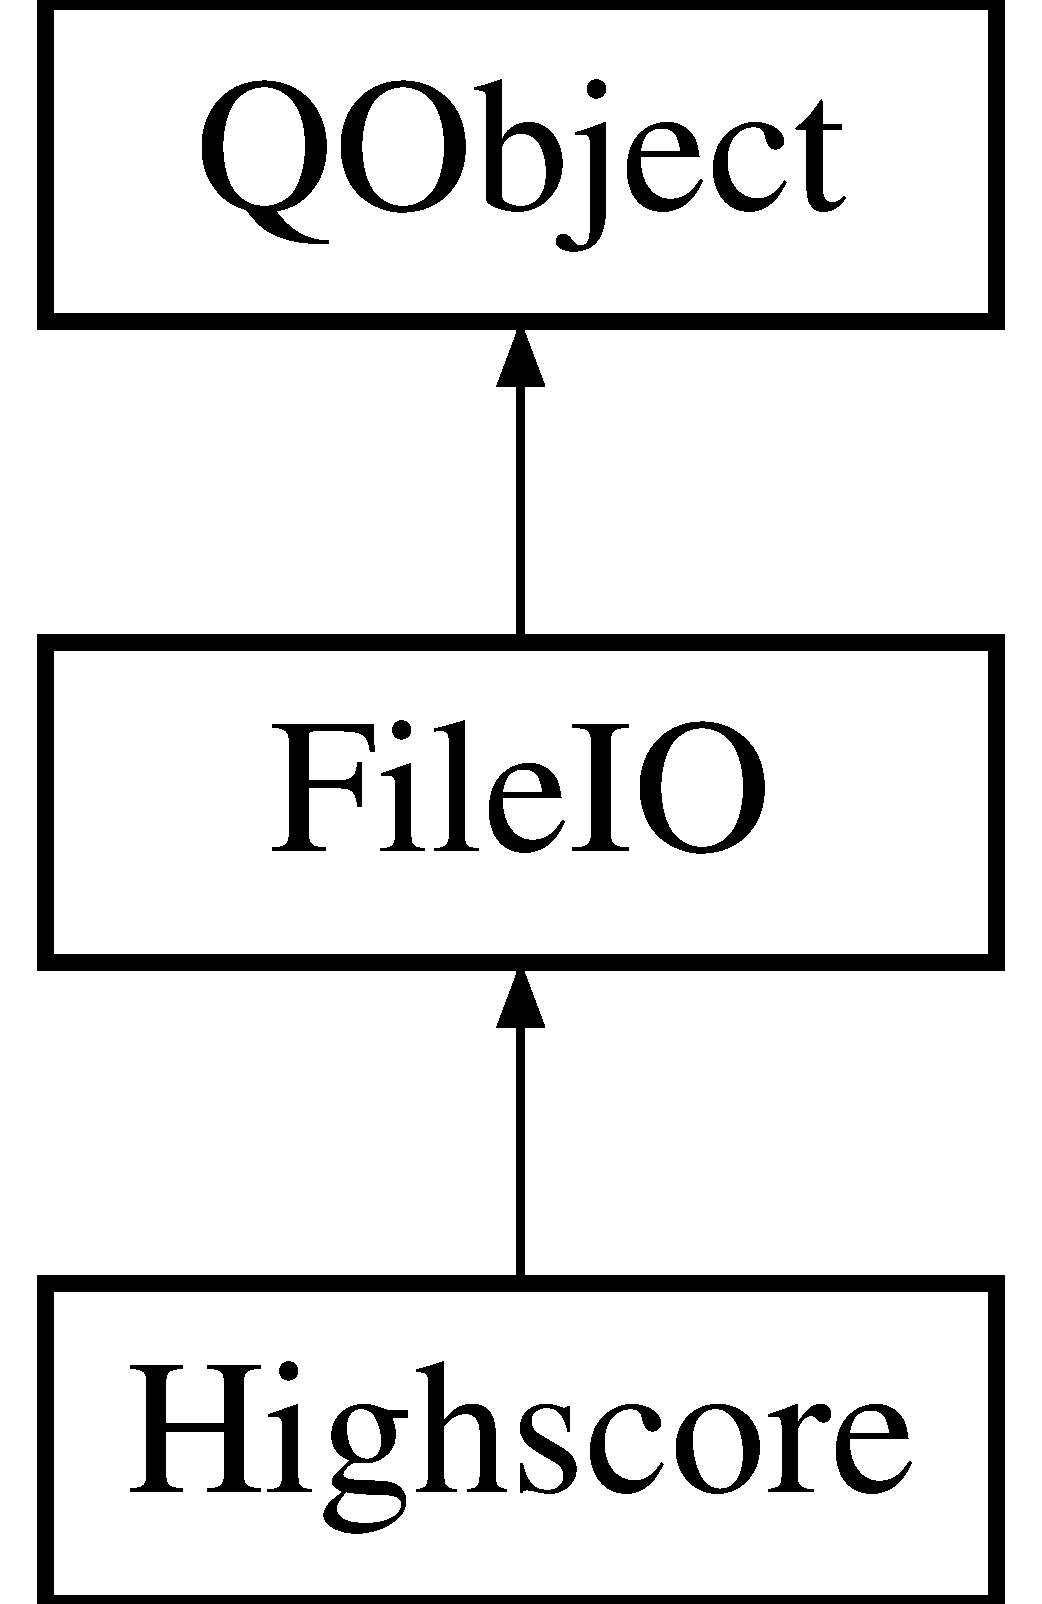
\includegraphics[height=3.000000cm]{class_highscore}
\end{center}
\end{figure}
\subsection*{Public Member Functions}
\begin{DoxyCompactItemize}
\item 
\hyperlink{class_highscore_ab760f6092405a654479f34107dc38beb}{Highscore} (Q\+Object $\ast$parent=0)
\item 
\hyperlink{class_highscore_ac22dda9e0f6aeceab3c61035d6e1be5c}{$\sim$\+Highscore} ()
\end{DoxyCompactItemize}
\subsection*{Additional Inherited Members}


\subsection{Detailed Description}
The \hyperlink{class_highscore}{Highscore} is only a semantic class. We want to clarify that this file\+I\+O is a \hyperlink{class_highscore}{Highscore}. 

\subsection{Constructor \& Destructor Documentation}
\hypertarget{class_highscore_ab760f6092405a654479f34107dc38beb}{}\index{Highscore@{Highscore}!Highscore@{Highscore}}
\index{Highscore@{Highscore}!Highscore@{Highscore}}
\subsubsection[{Highscore}]{\setlength{\rightskip}{0pt plus 5cm}Highscore\+::\+Highscore (
\begin{DoxyParamCaption}
\item[{Q\+Object $\ast$}]{parent = {\ttfamily 0}}
\end{DoxyParamCaption}
)\hspace{0.3cm}{\ttfamily [explicit]}}\label{class_highscore_ab760f6092405a654479f34107dc38beb}
\hypertarget{class_highscore_ac22dda9e0f6aeceab3c61035d6e1be5c}{}\index{Highscore@{Highscore}!````~Highscore@{$\sim$\+Highscore}}
\index{````~Highscore@{$\sim$\+Highscore}!Highscore@{Highscore}}
\subsubsection[{$\sim$\+Highscore}]{\setlength{\rightskip}{0pt plus 5cm}Highscore\+::$\sim$\+Highscore (
\begin{DoxyParamCaption}
{}
\end{DoxyParamCaption}
)}\label{class_highscore_ac22dda9e0f6aeceab3c61035d6e1be5c}


The documentation for this class was generated from the following files\+:\begin{DoxyCompactItemize}
\item 
Game-\/\+Programming-\/\+W\+S2014/gem\+Illuminator/\hyperlink{highscore_8h}{highscore.\+h}\item 
Game-\/\+Programming-\/\+W\+S2014/gem\+Illuminator/\hyperlink{highscore_8cpp}{highscore.\+cpp}\end{DoxyCompactItemize}

\hypertarget{class_light_ray}{\section{Light\+Ray Class Reference}
\label{class_light_ray}\index{Light\+Ray@{Light\+Ray}}
}


The \hyperlink{class_light_ray}{Light\+Ray} class describes the lightrays sent into \hyperlink{class_scene}{Scene}.  Because Light\+Rays are sent into \hyperlink{class_scene}{Scene} right after creation, they are more lines but rays. Rays are organized as a tree, a ray owns all of its \hyperlink{class_light_ray_a6673a77eb8fcd32dcfde26a1b112d303}{successors()}. Most of the game logic is still done within \hyperlink{class_light_ray_acf06a71a307433fa5b220baccf809e64}{Light\+Ray\+::update()}.  




{\ttfamily \#include $<$lightray.\+h$>$}

Inheritance diagram for Light\+Ray\+:\begin{figure}[H]
\begin{center}
\leavevmode
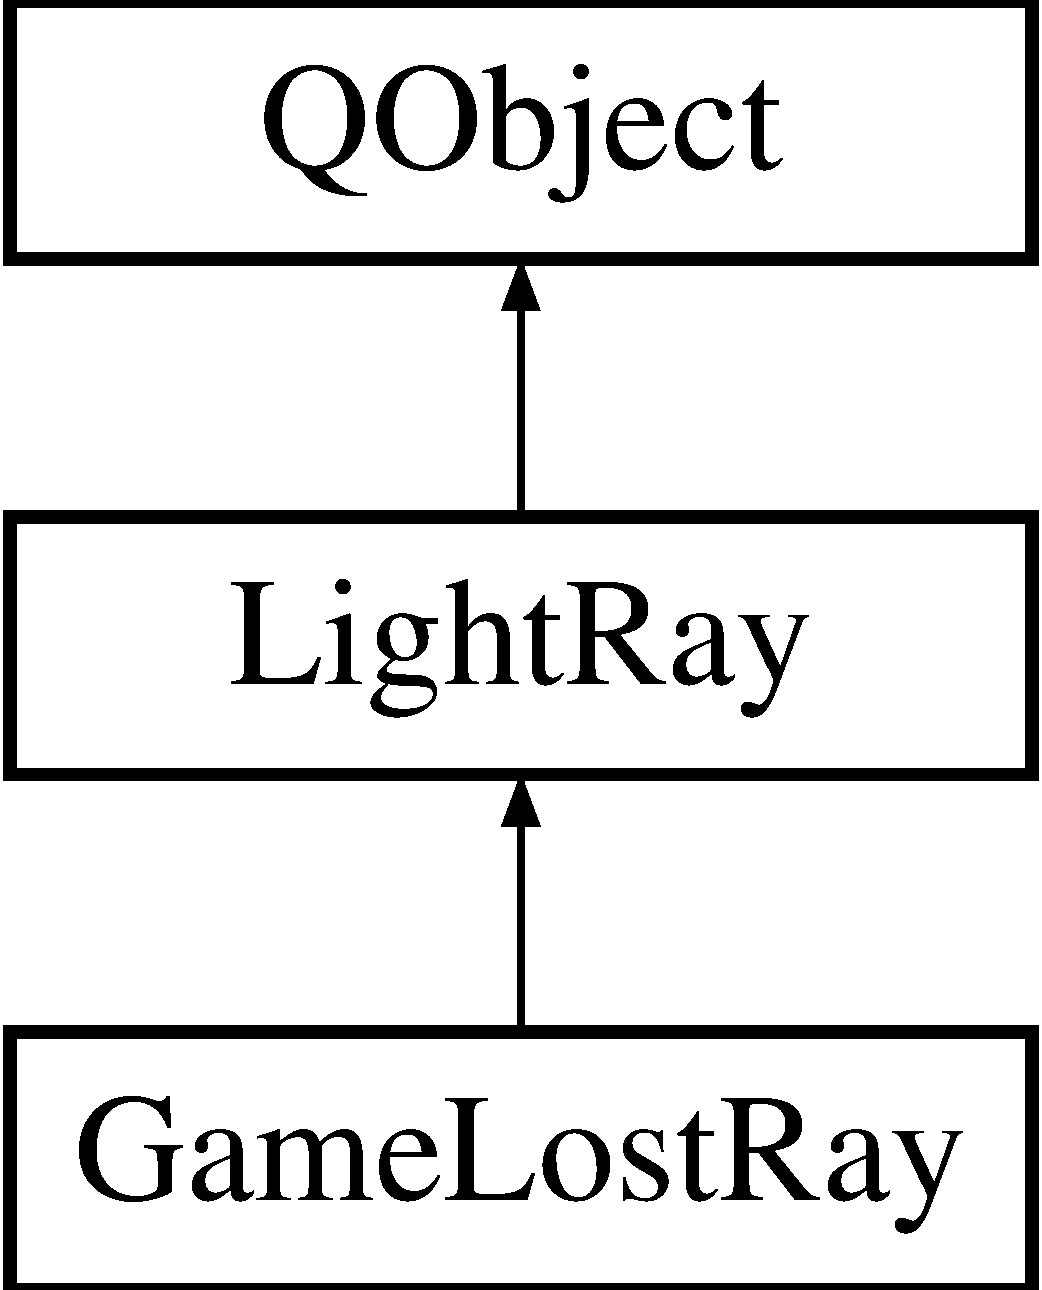
\includegraphics[height=3.000000cm]{class_light_ray}
\end{center}
\end{figure}
\subsection*{Public Slots}
\begin{DoxyCompactItemize}
\item 
const Q\+Vector3\+D \& \hyperlink{class_light_ray_a70d3d18bbecdf54dc399df5112ca024a}{start\+Position} () const 
\item 
void \hyperlink{class_light_ray_a1db98f630b5a18bb297936fc5c8f25fb}{set\+Start\+Position} (const Q\+Vector3\+D \&position)
\item 
const Q\+Vector3\+D \& \hyperlink{class_light_ray_a13026c9fc18cf7fc2d53832223172f13}{end\+Position} () const 
\item 
void \hyperlink{class_light_ray_a5b9d55f5a6bed4b610f1bc294905dd64}{set\+End\+Position} (const Q\+Vector3\+D \&position)
\item 
const Q\+Vector3\+D \& \hyperlink{class_light_ray_af2c247c9b2cc33b4b18ead8e1b12c697}{direction} () const 
\item 
const Q\+Vector3\+D \& \hyperlink{class_light_ray_a1a0dfa514a6c350b78e20903d2fde5c4}{normalized\+Direction} () const 
\item 
const Q\+Vector3\+D \& \hyperlink{class_light_ray_ae816ba62186298d8900e4617034d1d66}{color} () const 
\item 
void \hyperlink{class_light_ray_a607addd328ae2b935d21e093ae15bcd4}{set\+Color} (const Q\+Vector3\+D \&color)
\item 
\hyperlink{class_player}{Player} $\ast$ \hyperlink{class_light_ray_ab2e0d1d08c23a451b83907d61af4297a}{player} () const 
\item 
void \hyperlink{class_light_ray_a3720775f0e8d6c5a8041fd6a7b371dad}{set\+Player} (\hyperlink{class_player}{Player} $\ast$attached\+Player)
\item 
\hyperlink{class_scene}{Scene} $\ast$ \hyperlink{class_light_ray_a7ad5ff6f8863759c2183c95ba8914dfc}{scene} () const 
\item 
void \hyperlink{class_light_ray_a82577f82a77e84b81bd1b722a00bde54}{set\+Scene} (\hyperlink{class_scene}{Scene} $\ast$owning\+Scene)
\item 
bool \hyperlink{class_light_ray_a86e10593e7c2e3a4bbbbf817dd774c27}{is\+Static} () const 
\item 
void \hyperlink{class_light_ray_a6694333616a4d172f1c1bcb4ccbe1587}{set\+Static} ()
\item 
\hyperlink{class_light_ray}{Light\+Ray} $\ast$ \hyperlink{class_light_ray_ad7a12f31f9f84adc155211009a677d77}{selected\+Successor} ()
\begin{DoxyCompactList}\small\item\em Returns the ray the player should move on after reaching end of current ray. In case no successors exists they will be calculated using \hyperlink{class_light_ray_a1711b1964da22ce4083740adc2233780}{calculate\+Successors()} \end{DoxyCompactList}\item 
void \hyperlink{class_light_ray_a2644a596af5de9b41f770131b5c2b0eb}{set\+Selected\+Successor} (\hyperlink{class_light_ray}{Light\+Ray} $\ast$successor)
\item 
const \hyperlink{singleton_q_list}{Q\+List}$<$ \hyperlink{class_light_ray}{Light\+Ray} $\ast$ $>$ \& \hyperlink{class_light_ray_a6673a77eb8fcd32dcfde26a1b112d303}{successors} ()
\end{DoxyCompactItemize}
\subsection*{Signals}
\begin{DoxyCompactItemize}
\item 
void \hyperlink{class_light_ray_a4c9bff5b766f6ba5f4a265cd6aa64958}{color\+Changed} ()
\item 
void \hyperlink{class_light_ray_a5be9eb60aae11d0c24e7db4aa1f89b6c}{start\+Position\+Changed} ()
\item 
void \hyperlink{class_light_ray_a146c3e8249de30de6340fffbf0c1a4d6}{end\+Position\+Changed} ()
\item 
void \hyperlink{class_light_ray_a7b14272e752393259f0b645d92113782}{player\+Changed} ()
\item 
void \hyperlink{class_light_ray_aeea833ba9fe0fe8a3810ba002c3dbec4}{scene\+Changed} ()
\end{DoxyCompactItemize}
\subsection*{Public Member Functions}
\begin{DoxyCompactItemize}
\item 
\hyperlink{class_light_ray_a311f25dc81f2acfe6bc9f7379f76e6fe}{Light\+Ray} (Q\+Object $\ast$parent=0)
\item 
virtual \hyperlink{class_light_ray_a1ec27c859b1851ef680f803ae0555f17}{$\sim$\+Light\+Ray} ()
\item 
virtual void \hyperlink{class_light_ray_acf06a71a307433fa5b220baccf809e64}{update} (int time\+Difference)
\begin{DoxyCompactList}\small\item\em Updates our game. The player will be moved. \end{DoxyCompactList}\item 
Q\+Vector3\+D \hyperlink{class_light_ray_ab8723690d8af8cb9b4ba339eff784135}{normalized\+Orthogonal\+Vector} () const 
\begin{DoxyCompactList}\small\item\em Calculates a normalized vector that is orthogonal to direction(). \end{DoxyCompactList}\item 
Q\+Vector3\+D \hyperlink{class_light_ray_afe5d6813717569166a2c2ca29b2bc923}{calculate\+Color} ()
\begin{DoxyCompactList}\small\item\em calculate\+Successor\+Color calculates the successor color based on its normalized direction The color values are approximately in the range between 0.\+1 and 0.\+8 \end{DoxyCompactList}\end{DoxyCompactItemize}
\subsection*{Protected Member Functions}
\begin{DoxyCompactItemize}
\item 
bool \hyperlink{class_light_ray_ad2f26e29e0781597f7bf106396ba2fb7}{is\+Player\+Before\+Collision\+Point} ()
\item 
void \hyperlink{class_light_ray_a1711b1964da22ce4083740adc2233780}{calculate\+Successors} ()
\item 
\hyperlink{class_abstract_gem}{Abstract\+Gem} $\ast$ \hyperlink{class_light_ray_a9db8f3d965dec84c167b6634bee842f4}{colliding\+Gem} () const 
\item 
void \hyperlink{class_light_ray_a87c45492f6508b5c1adf8300babf8eeb}{set\+Colliding\+Gem} (\hyperlink{class_abstract_gem}{Abstract\+Gem} $\ast$gem)
\end{DoxyCompactItemize}
\subsection*{Protected Attributes}
\begin{DoxyCompactItemize}
\item 
\hyperlink{class_abstract_gem}{Abstract\+Gem} $\ast$ \hyperlink{class_light_ray_ac11396a5ac4a0899ca4bad5d88300fdd}{m\+\_\+colliding\+Gem}
\item 
\hyperlink{class_light_ray_data}{Light\+Ray\+Data} $\ast$ \hyperlink{class_light_ray_acba0c9beeba8ea2863a022910d4ffc34}{m\+\_\+data}
\item 
\hyperlink{singleton_q_list}{Q\+List}$<$ \hyperlink{class_light_ray}{Light\+Ray} $\ast$ $>$ $\ast$ \hyperlink{class_light_ray_a669e04446c77fc44bee41146c1883356}{m\+\_\+successors}
\item 
\hyperlink{class_light_ray}{Light\+Ray} $\ast$ \hyperlink{class_light_ray_a9e430528b861007696716fbd054c9de3}{m\+\_\+selected\+Successor}
\item 
bool \hyperlink{class_light_ray_af44c254c7782710304489afdabd5303a}{m\+\_\+is\+Static}
\item 
\hyperlink{class_player}{Player} $\ast$ \hyperlink{class_light_ray_a55cf457d13b240178933f0a73d6f7b2b}{m\+\_\+player}
\item 
\hyperlink{class_scene}{Scene} $\ast$ \hyperlink{class_light_ray_a9f99d6386ed92c979889f38b5348d628}{m\+\_\+scene}
\end{DoxyCompactItemize}


\subsection{Detailed Description}
The \hyperlink{class_light_ray}{Light\+Ray} class describes the lightrays sent into \hyperlink{class_scene}{Scene}.  Because Light\+Rays are sent into \hyperlink{class_scene}{Scene} right after creation, they are more lines but rays. Rays are organized as a tree, a ray owns all of its \hyperlink{class_light_ray_a6673a77eb8fcd32dcfde26a1b112d303}{successors()}. Most of the game logic is still done within \hyperlink{class_light_ray_acf06a71a307433fa5b220baccf809e64}{Light\+Ray\+::update()}. 

\subsection{Constructor \& Destructor Documentation}
\hypertarget{class_light_ray_a311f25dc81f2acfe6bc9f7379f76e6fe}{\index{Light\+Ray@{Light\+Ray}!Light\+Ray@{Light\+Ray}}
\index{Light\+Ray@{Light\+Ray}!Light\+Ray@{Light\+Ray}}
\subsubsection[{Light\+Ray}]{\setlength{\rightskip}{0pt plus 5cm}Light\+Ray\+::\+Light\+Ray (
\begin{DoxyParamCaption}
\item[{Q\+Object $\ast$}]{parent = {\ttfamily 0}}
\end{DoxyParamCaption}
)\hspace{0.3cm}{\ttfamily [explicit]}}}\label{class_light_ray_a311f25dc81f2acfe6bc9f7379f76e6fe}
\hypertarget{class_light_ray_a1ec27c859b1851ef680f803ae0555f17}{\index{Light\+Ray@{Light\+Ray}!````~Light\+Ray@{$\sim$\+Light\+Ray}}
\index{````~Light\+Ray@{$\sim$\+Light\+Ray}!Light\+Ray@{Light\+Ray}}
\subsubsection[{$\sim$\+Light\+Ray}]{\setlength{\rightskip}{0pt plus 5cm}Light\+Ray\+::$\sim$\+Light\+Ray (
\begin{DoxyParamCaption}
{}
\end{DoxyParamCaption}
)\hspace{0.3cm}{\ttfamily [virtual]}}}\label{class_light_ray_a1ec27c859b1851ef680f803ae0555f17}


\subsection{Member Function Documentation}
\hypertarget{class_light_ray_afe5d6813717569166a2c2ca29b2bc923}{\index{Light\+Ray@{Light\+Ray}!calculate\+Color@{calculate\+Color}}
\index{calculate\+Color@{calculate\+Color}!Light\+Ray@{Light\+Ray}}
\subsubsection[{calculate\+Color}]{\setlength{\rightskip}{0pt plus 5cm}Q\+Vector3\+D Light\+Ray\+::calculate\+Color (
\begin{DoxyParamCaption}
{}
\end{DoxyParamCaption}
)}}\label{class_light_ray_afe5d6813717569166a2c2ca29b2bc923}


calculate\+Successor\+Color calculates the successor color based on its normalized direction The color values are approximately in the range between 0.\+1 and 0.\+8 

\begin{DoxyReturn}{Returns}
The calculated color 
\end{DoxyReturn}
\hypertarget{class_light_ray_a1711b1964da22ce4083740adc2233780}{\index{Light\+Ray@{Light\+Ray}!calculate\+Successors@{calculate\+Successors}}
\index{calculate\+Successors@{calculate\+Successors}!Light\+Ray@{Light\+Ray}}
\subsubsection[{calculate\+Successors}]{\setlength{\rightskip}{0pt plus 5cm}void Light\+Ray\+::calculate\+Successors (
\begin{DoxyParamCaption}
{}
\end{DoxyParamCaption}
)\hspace{0.3cm}{\ttfamily [protected]}}}\label{class_light_ray_a1711b1964da22ce4083740adc2233780}
\hypertarget{class_light_ray_a9db8f3d965dec84c167b6634bee842f4}{\index{Light\+Ray@{Light\+Ray}!colliding\+Gem@{colliding\+Gem}}
\index{colliding\+Gem@{colliding\+Gem}!Light\+Ray@{Light\+Ray}}
\subsubsection[{colliding\+Gem}]{\setlength{\rightskip}{0pt plus 5cm}{\bf Abstract\+Gem} $\ast$ Light\+Ray\+::colliding\+Gem (
\begin{DoxyParamCaption}
{}
\end{DoxyParamCaption}
) const\hspace{0.3cm}{\ttfamily [protected]}}}\label{class_light_ray_a9db8f3d965dec84c167b6634bee842f4}
\hypertarget{class_light_ray_ae816ba62186298d8900e4617034d1d66}{\index{Light\+Ray@{Light\+Ray}!color@{color}}
\index{color@{color}!Light\+Ray@{Light\+Ray}}
\subsubsection[{color}]{\setlength{\rightskip}{0pt plus 5cm}const Q\+Vector3\+D\& Light\+Ray\+::color (
\begin{DoxyParamCaption}
{}
\end{DoxyParamCaption}
) const\hspace{0.3cm}{\ttfamily [slot]}}}\label{class_light_ray_ae816ba62186298d8900e4617034d1d66}
\hypertarget{class_light_ray_a4c9bff5b766f6ba5f4a265cd6aa64958}{\index{Light\+Ray@{Light\+Ray}!color\+Changed@{color\+Changed}}
\index{color\+Changed@{color\+Changed}!Light\+Ray@{Light\+Ray}}
\subsubsection[{color\+Changed}]{\setlength{\rightskip}{0pt plus 5cm}void Light\+Ray\+::color\+Changed (
\begin{DoxyParamCaption}
{}
\end{DoxyParamCaption}
)\hspace{0.3cm}{\ttfamily [signal]}}}\label{class_light_ray_a4c9bff5b766f6ba5f4a265cd6aa64958}
\hypertarget{class_light_ray_af2c247c9b2cc33b4b18ead8e1b12c697}{\index{Light\+Ray@{Light\+Ray}!direction@{direction}}
\index{direction@{direction}!Light\+Ray@{Light\+Ray}}
\subsubsection[{direction}]{\setlength{\rightskip}{0pt plus 5cm}const Q\+Vector3\+D\& Light\+Ray\+::direction (
\begin{DoxyParamCaption}
{}
\end{DoxyParamCaption}
) const\hspace{0.3cm}{\ttfamily [slot]}}}\label{class_light_ray_af2c247c9b2cc33b4b18ead8e1b12c697}
\hypertarget{class_light_ray_a13026c9fc18cf7fc2d53832223172f13}{\index{Light\+Ray@{Light\+Ray}!end\+Position@{end\+Position}}
\index{end\+Position@{end\+Position}!Light\+Ray@{Light\+Ray}}
\subsubsection[{end\+Position}]{\setlength{\rightskip}{0pt plus 5cm}const Q\+Vector3\+D\& Light\+Ray\+::end\+Position (
\begin{DoxyParamCaption}
{}
\end{DoxyParamCaption}
) const\hspace{0.3cm}{\ttfamily [slot]}}}\label{class_light_ray_a13026c9fc18cf7fc2d53832223172f13}
\hypertarget{class_light_ray_a146c3e8249de30de6340fffbf0c1a4d6}{\index{Light\+Ray@{Light\+Ray}!end\+Position\+Changed@{end\+Position\+Changed}}
\index{end\+Position\+Changed@{end\+Position\+Changed}!Light\+Ray@{Light\+Ray}}
\subsubsection[{end\+Position\+Changed}]{\setlength{\rightskip}{0pt plus 5cm}void Light\+Ray\+::end\+Position\+Changed (
\begin{DoxyParamCaption}
{}
\end{DoxyParamCaption}
)\hspace{0.3cm}{\ttfamily [signal]}}}\label{class_light_ray_a146c3e8249de30de6340fffbf0c1a4d6}
\hypertarget{class_light_ray_ad2f26e29e0781597f7bf106396ba2fb7}{\index{Light\+Ray@{Light\+Ray}!is\+Player\+Before\+Collision\+Point@{is\+Player\+Before\+Collision\+Point}}
\index{is\+Player\+Before\+Collision\+Point@{is\+Player\+Before\+Collision\+Point}!Light\+Ray@{Light\+Ray}}
\subsubsection[{is\+Player\+Before\+Collision\+Point}]{\setlength{\rightskip}{0pt plus 5cm}bool Light\+Ray\+::is\+Player\+Before\+Collision\+Point (
\begin{DoxyParamCaption}
{}
\end{DoxyParamCaption}
)\hspace{0.3cm}{\ttfamily [protected]}}}\label{class_light_ray_ad2f26e29e0781597f7bf106396ba2fb7}
\hypertarget{class_light_ray_a86e10593e7c2e3a4bbbbf817dd774c27}{\index{Light\+Ray@{Light\+Ray}!is\+Static@{is\+Static}}
\index{is\+Static@{is\+Static}!Light\+Ray@{Light\+Ray}}
\subsubsection[{is\+Static}]{\setlength{\rightskip}{0pt plus 5cm}bool Light\+Ray\+::is\+Static (
\begin{DoxyParamCaption}
{}
\end{DoxyParamCaption}
) const\hspace{0.3cm}{\ttfamily [slot]}}}\label{class_light_ray_a86e10593e7c2e3a4bbbbf817dd774c27}
\hypertarget{class_light_ray_a1a0dfa514a6c350b78e20903d2fde5c4}{\index{Light\+Ray@{Light\+Ray}!normalized\+Direction@{normalized\+Direction}}
\index{normalized\+Direction@{normalized\+Direction}!Light\+Ray@{Light\+Ray}}
\subsubsection[{normalized\+Direction}]{\setlength{\rightskip}{0pt plus 5cm}const Q\+Vector3\+D\& Light\+Ray\+::normalized\+Direction (
\begin{DoxyParamCaption}
{}
\end{DoxyParamCaption}
) const\hspace{0.3cm}{\ttfamily [slot]}}}\label{class_light_ray_a1a0dfa514a6c350b78e20903d2fde5c4}
\hypertarget{class_light_ray_ab8723690d8af8cb9b4ba339eff784135}{\index{Light\+Ray@{Light\+Ray}!normalized\+Orthogonal\+Vector@{normalized\+Orthogonal\+Vector}}
\index{normalized\+Orthogonal\+Vector@{normalized\+Orthogonal\+Vector}!Light\+Ray@{Light\+Ray}}
\subsubsection[{normalized\+Orthogonal\+Vector}]{\setlength{\rightskip}{0pt plus 5cm}Q\+Vector3\+D Light\+Ray\+::normalized\+Orthogonal\+Vector (
\begin{DoxyParamCaption}
{}
\end{DoxyParamCaption}
) const}}\label{class_light_ray_ab8723690d8af8cb9b4ba339eff784135}


Calculates a normalized vector that is orthogonal to direction(). 

\begin{DoxyReturn}{Returns}

\end{DoxyReturn}
\hypertarget{class_light_ray_ab2e0d1d08c23a451b83907d61af4297a}{\index{Light\+Ray@{Light\+Ray}!player@{player}}
\index{player@{player}!Light\+Ray@{Light\+Ray}}
\subsubsection[{player}]{\setlength{\rightskip}{0pt plus 5cm}{\bf Player}$\ast$ Light\+Ray\+::player (
\begin{DoxyParamCaption}
{}
\end{DoxyParamCaption}
) const\hspace{0.3cm}{\ttfamily [slot]}}}\label{class_light_ray_ab2e0d1d08c23a451b83907d61af4297a}
\hypertarget{class_light_ray_a7b14272e752393259f0b645d92113782}{\index{Light\+Ray@{Light\+Ray}!player\+Changed@{player\+Changed}}
\index{player\+Changed@{player\+Changed}!Light\+Ray@{Light\+Ray}}
\subsubsection[{player\+Changed}]{\setlength{\rightskip}{0pt plus 5cm}void Light\+Ray\+::player\+Changed (
\begin{DoxyParamCaption}
{}
\end{DoxyParamCaption}
)\hspace{0.3cm}{\ttfamily [signal]}}}\label{class_light_ray_a7b14272e752393259f0b645d92113782}
\hypertarget{class_light_ray_a7ad5ff6f8863759c2183c95ba8914dfc}{\index{Light\+Ray@{Light\+Ray}!scene@{scene}}
\index{scene@{scene}!Light\+Ray@{Light\+Ray}}
\subsubsection[{scene}]{\setlength{\rightskip}{0pt plus 5cm}{\bf Scene}$\ast$ Light\+Ray\+::scene (
\begin{DoxyParamCaption}
{}
\end{DoxyParamCaption}
) const\hspace{0.3cm}{\ttfamily [slot]}}}\label{class_light_ray_a7ad5ff6f8863759c2183c95ba8914dfc}
\hypertarget{class_light_ray_aeea833ba9fe0fe8a3810ba002c3dbec4}{\index{Light\+Ray@{Light\+Ray}!scene\+Changed@{scene\+Changed}}
\index{scene\+Changed@{scene\+Changed}!Light\+Ray@{Light\+Ray}}
\subsubsection[{scene\+Changed}]{\setlength{\rightskip}{0pt plus 5cm}void Light\+Ray\+::scene\+Changed (
\begin{DoxyParamCaption}
{}
\end{DoxyParamCaption}
)\hspace{0.3cm}{\ttfamily [signal]}}}\label{class_light_ray_aeea833ba9fe0fe8a3810ba002c3dbec4}
\hypertarget{class_light_ray_ad7a12f31f9f84adc155211009a677d77}{\index{Light\+Ray@{Light\+Ray}!selected\+Successor@{selected\+Successor}}
\index{selected\+Successor@{selected\+Successor}!Light\+Ray@{Light\+Ray}}
\subsubsection[{selected\+Successor}]{\setlength{\rightskip}{0pt plus 5cm}{\bf Light\+Ray} $\ast$ Light\+Ray\+::selected\+Successor (
\begin{DoxyParamCaption}
{}
\end{DoxyParamCaption}
)\hspace{0.3cm}{\ttfamily [slot]}}}\label{class_light_ray_ad7a12f31f9f84adc155211009a677d77}


Returns the ray the player should move on after reaching end of current ray. In case no successors exists they will be calculated using \hyperlink{class_light_ray_a1711b1964da22ce4083740adc2233780}{calculate\+Successors()} 

\begin{DoxyReturn}{Returns}

\end{DoxyReturn}
\hypertarget{class_light_ray_a87c45492f6508b5c1adf8300babf8eeb}{\index{Light\+Ray@{Light\+Ray}!set\+Colliding\+Gem@{set\+Colliding\+Gem}}
\index{set\+Colliding\+Gem@{set\+Colliding\+Gem}!Light\+Ray@{Light\+Ray}}
\subsubsection[{set\+Colliding\+Gem}]{\setlength{\rightskip}{0pt plus 5cm}void Light\+Ray\+::set\+Colliding\+Gem (
\begin{DoxyParamCaption}
\item[{{\bf Abstract\+Gem} $\ast$}]{gem}
\end{DoxyParamCaption}
)\hspace{0.3cm}{\ttfamily [protected]}}}\label{class_light_ray_a87c45492f6508b5c1adf8300babf8eeb}
\hypertarget{class_light_ray_a607addd328ae2b935d21e093ae15bcd4}{\index{Light\+Ray@{Light\+Ray}!set\+Color@{set\+Color}}
\index{set\+Color@{set\+Color}!Light\+Ray@{Light\+Ray}}
\subsubsection[{set\+Color}]{\setlength{\rightskip}{0pt plus 5cm}void Light\+Ray\+::set\+Color (
\begin{DoxyParamCaption}
\item[{const Q\+Vector3\+D \&}]{color}
\end{DoxyParamCaption}
)\hspace{0.3cm}{\ttfamily [slot]}}}\label{class_light_ray_a607addd328ae2b935d21e093ae15bcd4}
\hypertarget{class_light_ray_a5b9d55f5a6bed4b610f1bc294905dd64}{\index{Light\+Ray@{Light\+Ray}!set\+End\+Position@{set\+End\+Position}}
\index{set\+End\+Position@{set\+End\+Position}!Light\+Ray@{Light\+Ray}}
\subsubsection[{set\+End\+Position}]{\setlength{\rightskip}{0pt plus 5cm}void Light\+Ray\+::set\+End\+Position (
\begin{DoxyParamCaption}
\item[{const Q\+Vector3\+D \&}]{position}
\end{DoxyParamCaption}
)\hspace{0.3cm}{\ttfamily [slot]}}}\label{class_light_ray_a5b9d55f5a6bed4b610f1bc294905dd64}
\hypertarget{class_light_ray_a3720775f0e8d6c5a8041fd6a7b371dad}{\index{Light\+Ray@{Light\+Ray}!set\+Player@{set\+Player}}
\index{set\+Player@{set\+Player}!Light\+Ray@{Light\+Ray}}
\subsubsection[{set\+Player}]{\setlength{\rightskip}{0pt plus 5cm}void Light\+Ray\+::set\+Player (
\begin{DoxyParamCaption}
\item[{{\bf Player} $\ast$}]{attached\+Player}
\end{DoxyParamCaption}
)\hspace{0.3cm}{\ttfamily [slot]}}}\label{class_light_ray_a3720775f0e8d6c5a8041fd6a7b371dad}
\hypertarget{class_light_ray_a82577f82a77e84b81bd1b722a00bde54}{\index{Light\+Ray@{Light\+Ray}!set\+Scene@{set\+Scene}}
\index{set\+Scene@{set\+Scene}!Light\+Ray@{Light\+Ray}}
\subsubsection[{set\+Scene}]{\setlength{\rightskip}{0pt plus 5cm}void Light\+Ray\+::set\+Scene (
\begin{DoxyParamCaption}
\item[{{\bf Scene} $\ast$}]{owning\+Scene}
\end{DoxyParamCaption}
)\hspace{0.3cm}{\ttfamily [slot]}}}\label{class_light_ray_a82577f82a77e84b81bd1b722a00bde54}
\hypertarget{class_light_ray_a2644a596af5de9b41f770131b5c2b0eb}{\index{Light\+Ray@{Light\+Ray}!set\+Selected\+Successor@{set\+Selected\+Successor}}
\index{set\+Selected\+Successor@{set\+Selected\+Successor}!Light\+Ray@{Light\+Ray}}
\subsubsection[{set\+Selected\+Successor}]{\setlength{\rightskip}{0pt plus 5cm}void Light\+Ray\+::set\+Selected\+Successor (
\begin{DoxyParamCaption}
\item[{{\bf Light\+Ray} $\ast$}]{successor}
\end{DoxyParamCaption}
)\hspace{0.3cm}{\ttfamily [slot]}}}\label{class_light_ray_a2644a596af5de9b41f770131b5c2b0eb}
\hypertarget{class_light_ray_a1db98f630b5a18bb297936fc5c8f25fb}{\index{Light\+Ray@{Light\+Ray}!set\+Start\+Position@{set\+Start\+Position}}
\index{set\+Start\+Position@{set\+Start\+Position}!Light\+Ray@{Light\+Ray}}
\subsubsection[{set\+Start\+Position}]{\setlength{\rightskip}{0pt plus 5cm}void Light\+Ray\+::set\+Start\+Position (
\begin{DoxyParamCaption}
\item[{const Q\+Vector3\+D \&}]{position}
\end{DoxyParamCaption}
)\hspace{0.3cm}{\ttfamily [slot]}}}\label{class_light_ray_a1db98f630b5a18bb297936fc5c8f25fb}
\hypertarget{class_light_ray_a6694333616a4d172f1c1bcb4ccbe1587}{\index{Light\+Ray@{Light\+Ray}!set\+Static@{set\+Static}}
\index{set\+Static@{set\+Static}!Light\+Ray@{Light\+Ray}}
\subsubsection[{set\+Static}]{\setlength{\rightskip}{0pt plus 5cm}void Light\+Ray\+::set\+Static (
\begin{DoxyParamCaption}
{}
\end{DoxyParamCaption}
)\hspace{0.3cm}{\ttfamily [slot]}}}\label{class_light_ray_a6694333616a4d172f1c1bcb4ccbe1587}
\hypertarget{class_light_ray_a70d3d18bbecdf54dc399df5112ca024a}{\index{Light\+Ray@{Light\+Ray}!start\+Position@{start\+Position}}
\index{start\+Position@{start\+Position}!Light\+Ray@{Light\+Ray}}
\subsubsection[{start\+Position}]{\setlength{\rightskip}{0pt plus 5cm}const Q\+Vector3\+D\& Light\+Ray\+::start\+Position (
\begin{DoxyParamCaption}
{}
\end{DoxyParamCaption}
) const\hspace{0.3cm}{\ttfamily [slot]}}}\label{class_light_ray_a70d3d18bbecdf54dc399df5112ca024a}
\hypertarget{class_light_ray_a5be9eb60aae11d0c24e7db4aa1f89b6c}{\index{Light\+Ray@{Light\+Ray}!start\+Position\+Changed@{start\+Position\+Changed}}
\index{start\+Position\+Changed@{start\+Position\+Changed}!Light\+Ray@{Light\+Ray}}
\subsubsection[{start\+Position\+Changed}]{\setlength{\rightskip}{0pt plus 5cm}void Light\+Ray\+::start\+Position\+Changed (
\begin{DoxyParamCaption}
{}
\end{DoxyParamCaption}
)\hspace{0.3cm}{\ttfamily [signal]}}}\label{class_light_ray_a5be9eb60aae11d0c24e7db4aa1f89b6c}
\hypertarget{class_light_ray_a6673a77eb8fcd32dcfde26a1b112d303}{\index{Light\+Ray@{Light\+Ray}!successors@{successors}}
\index{successors@{successors}!Light\+Ray@{Light\+Ray}}
\subsubsection[{successors}]{\setlength{\rightskip}{0pt plus 5cm}const {\bf Q\+List}$<$ {\bf Light\+Ray} $\ast$ $>$ \& Light\+Ray\+::successors (
\begin{DoxyParamCaption}
{}
\end{DoxyParamCaption}
)\hspace{0.3cm}{\ttfamily [slot]}}}\label{class_light_ray_a6673a77eb8fcd32dcfde26a1b112d303}
\hypertarget{class_light_ray_acf06a71a307433fa5b220baccf809e64}{\index{Light\+Ray@{Light\+Ray}!update@{update}}
\index{update@{update}!Light\+Ray@{Light\+Ray}}
\subsubsection[{update}]{\setlength{\rightskip}{0pt plus 5cm}void Light\+Ray\+::update (
\begin{DoxyParamCaption}
\item[{int}]{time\+Difference}
\end{DoxyParamCaption}
)\hspace{0.3cm}{\ttfamily [virtual]}}}\label{class_light_ray_acf06a71a307433fa5b220baccf809e64}


Updates our game. The player will be moved. 


\begin{DoxyParams}{Parameters}
{\em time\+Difference} & Time since last update in milliseconds. \\
\hline
\end{DoxyParams}


Reimplemented in \hyperlink{class_game_lost_ray_a417d814372891fe7595a7e745b7a9f0f}{Game\+Lost\+Ray}.



\subsection{Member Data Documentation}
\hypertarget{class_light_ray_ac11396a5ac4a0899ca4bad5d88300fdd}{\index{Light\+Ray@{Light\+Ray}!m\+\_\+colliding\+Gem@{m\+\_\+colliding\+Gem}}
\index{m\+\_\+colliding\+Gem@{m\+\_\+colliding\+Gem}!Light\+Ray@{Light\+Ray}}
\subsubsection[{m\+\_\+colliding\+Gem}]{\setlength{\rightskip}{0pt plus 5cm}{\bf Abstract\+Gem}$\ast$ Light\+Ray\+::m\+\_\+colliding\+Gem\hspace{0.3cm}{\ttfamily [protected]}}}\label{class_light_ray_ac11396a5ac4a0899ca4bad5d88300fdd}
\hypertarget{class_light_ray_acba0c9beeba8ea2863a022910d4ffc34}{\index{Light\+Ray@{Light\+Ray}!m\+\_\+data@{m\+\_\+data}}
\index{m\+\_\+data@{m\+\_\+data}!Light\+Ray@{Light\+Ray}}
\subsubsection[{m\+\_\+data}]{\setlength{\rightskip}{0pt plus 5cm}{\bf Light\+Ray\+Data}$\ast$ Light\+Ray\+::m\+\_\+data\hspace{0.3cm}{\ttfamily [protected]}}}\label{class_light_ray_acba0c9beeba8ea2863a022910d4ffc34}
\hypertarget{class_light_ray_af44c254c7782710304489afdabd5303a}{\index{Light\+Ray@{Light\+Ray}!m\+\_\+is\+Static@{m\+\_\+is\+Static}}
\index{m\+\_\+is\+Static@{m\+\_\+is\+Static}!Light\+Ray@{Light\+Ray}}
\subsubsection[{m\+\_\+is\+Static}]{\setlength{\rightskip}{0pt plus 5cm}bool Light\+Ray\+::m\+\_\+is\+Static\hspace{0.3cm}{\ttfamily [protected]}}}\label{class_light_ray_af44c254c7782710304489afdabd5303a}
\hypertarget{class_light_ray_a55cf457d13b240178933f0a73d6f7b2b}{\index{Light\+Ray@{Light\+Ray}!m\+\_\+player@{m\+\_\+player}}
\index{m\+\_\+player@{m\+\_\+player}!Light\+Ray@{Light\+Ray}}
\subsubsection[{m\+\_\+player}]{\setlength{\rightskip}{0pt plus 5cm}{\bf Player}$\ast$ Light\+Ray\+::m\+\_\+player\hspace{0.3cm}{\ttfamily [protected]}}}\label{class_light_ray_a55cf457d13b240178933f0a73d6f7b2b}
\hypertarget{class_light_ray_a9f99d6386ed92c979889f38b5348d628}{\index{Light\+Ray@{Light\+Ray}!m\+\_\+scene@{m\+\_\+scene}}
\index{m\+\_\+scene@{m\+\_\+scene}!Light\+Ray@{Light\+Ray}}
\subsubsection[{m\+\_\+scene}]{\setlength{\rightskip}{0pt plus 5cm}{\bf Scene}$\ast$ Light\+Ray\+::m\+\_\+scene\hspace{0.3cm}{\ttfamily [protected]}}}\label{class_light_ray_a9f99d6386ed92c979889f38b5348d628}
\hypertarget{class_light_ray_a9e430528b861007696716fbd054c9de3}{\index{Light\+Ray@{Light\+Ray}!m\+\_\+selected\+Successor@{m\+\_\+selected\+Successor}}
\index{m\+\_\+selected\+Successor@{m\+\_\+selected\+Successor}!Light\+Ray@{Light\+Ray}}
\subsubsection[{m\+\_\+selected\+Successor}]{\setlength{\rightskip}{0pt plus 5cm}{\bf Light\+Ray}$\ast$ Light\+Ray\+::m\+\_\+selected\+Successor\hspace{0.3cm}{\ttfamily [protected]}}}\label{class_light_ray_a9e430528b861007696716fbd054c9de3}
\hypertarget{class_light_ray_a669e04446c77fc44bee41146c1883356}{\index{Light\+Ray@{Light\+Ray}!m\+\_\+successors@{m\+\_\+successors}}
\index{m\+\_\+successors@{m\+\_\+successors}!Light\+Ray@{Light\+Ray}}
\subsubsection[{m\+\_\+successors}]{\setlength{\rightskip}{0pt plus 5cm}{\bf Q\+List}$<${\bf Light\+Ray} $\ast$$>$$\ast$ Light\+Ray\+::m\+\_\+successors\hspace{0.3cm}{\ttfamily [protected]}}}\label{class_light_ray_a669e04446c77fc44bee41146c1883356}


The documentation for this class was generated from the following files\+:\begin{DoxyCompactItemize}
\item 
\hyperlink{lightray_8h}{lightray.\+h}\item 
\hyperlink{lightray_8cpp}{lightray.\+cpp}\end{DoxyCompactItemize}

\hypertarget{class_light_ray_data}{\section{Light\+Ray\+Data Class Reference}
\label{class_light_ray_data}\index{Light\+Ray\+Data@{Light\+Ray\+Data}}
}


The \hyperlink{class_light_ray_data}{Light\+Ray\+Data} class stores data of a \hyperlink{class_light_ray}{Light\+Ray}. The \hyperlink{class_light_ray_data}{Light\+Ray\+Data} doesn't inherit from Q\+Object, so it can be stored in Qt-\/\+Containers (currently only those require == or q\+Hash) by Value. Also the data can be copied easily.  




{\ttfamily \#include $<$lightraydata.\+h$>$}

\subsection*{Public Member Functions}
\begin{DoxyCompactItemize}
\item 
\hyperlink{class_light_ray_data_ac0cb11da1651f8ff7b8ed9d785b68a27}{Light\+Ray\+Data} ()
\item 
\hyperlink{class_light_ray_data_a50350aa163fd7c1a54f97cefafd2d2f7}{Light\+Ray\+Data} (const \hyperlink{class_light_ray}{Light\+Ray} \&light\+Ray)
\item 
\hyperlink{class_light_ray_data_a9344f139cafb257f61f4d800fbecd905}{Light\+Ray\+Data} (const \hyperlink{class_light_ray_data}{Light\+Ray\+Data} \&light\+Ray)
\item 
\hyperlink{class_light_ray_data_a6cd92465c9ba1da296d30a32487a6ac0}{$\sim$\+Light\+Ray\+Data} ()
\item 
Q\+Vector3\+D \hyperlink{class_light_ray_data_acada2319ae380a11a405817cd9cd3d65}{normalized\+Orthogonal\+Vector} () const 
\begin{DoxyCompactList}\small\item\em Calculates a normalized vector, that is orthogonal to \hyperlink{class_light_ray_data_aaecf9f1d378eebf6d577eaa588930a4f}{direction()}. \end{DoxyCompactList}\item 
const Q\+Vector3\+D \& \hyperlink{class_light_ray_data_a64a5b7f8d4c3af9cc3e8c1a6c6ea8c57}{color} () const 
\item 
void \hyperlink{class_light_ray_data_ad8fead207765a43bb1167e2ce95e85a4}{set\+Color} (const Q\+Vector3\+D \&\hyperlink{class_light_ray_data_a64a5b7f8d4c3af9cc3e8c1a6c6ea8c57}{color})
\item 
const Q\+Vector3\+D \& \hyperlink{class_light_ray_data_af040092e873e42d0d31f803452fc648e}{start\+Position} () const 
\item 
void \hyperlink{class_light_ray_data_a464a868047052152f375cb45ac476eb2}{set\+Start\+Position} (const Q\+Vector3\+D \&position)
\item 
const Q\+Vector3\+D \& \hyperlink{class_light_ray_data_ab47d397dcffe8a2c8da0cf4d8bbbd2bc}{end\+Position} () const 
\item 
void \hyperlink{class_light_ray_data_ad7ec7b96408f0fb7f603687c54804d3b}{set\+End\+Position} (const Q\+Vector3\+D \&position)
\item 
const Q\+Vector3\+D \& \hyperlink{class_light_ray_data_aaecf9f1d378eebf6d577eaa588930a4f}{direction} () const 
\item 
const Q\+Vector3\+D \& \hyperlink{class_light_ray_data_a791bbf3c85d32004d0d7d155cd248a43}{normalized\+Direction} () const 
\item 
\hyperlink{class_light_ray_data}{Light\+Ray\+Data} \& \hyperlink{class_light_ray_data_a2dc01f58929829517a90b1fc29f12942}{operator=} (const \hyperlink{class_light_ray_data}{Light\+Ray\+Data} \&light\+Ray)
\end{DoxyCompactItemize}
\subsection*{Protected Attributes}
\begin{DoxyCompactItemize}
\item 
Q\+Vector3\+D $\ast$ \hyperlink{class_light_ray_data_ae6ad9fa7cd9bc9db1837691c603e5eaa}{m\+\_\+color}
\item 
Q\+Vector3\+D $\ast$ \hyperlink{class_light_ray_data_a4a71e8787288d9e243c3c9dd744350ff}{m\+\_\+direction}
\item 
Q\+Vector3\+D $\ast$ \hyperlink{class_light_ray_data_af18cf984ba862735dcde2d77767c4bb2}{m\+\_\+direction\+Normalized}
\item 
Q\+Vector3\+D $\ast$ \hyperlink{class_light_ray_data_ab7228a576b4b1c0843641e3706a6cb35}{m\+\_\+end\+Position}
\item 
Q\+Vector3\+D $\ast$ \hyperlink{class_light_ray_data_a1da577bdf12b630015fca5d89712e479}{m\+\_\+start\+Position}
\end{DoxyCompactItemize}


\subsection{Detailed Description}
The \hyperlink{class_light_ray_data}{Light\+Ray\+Data} class stores data of a \hyperlink{class_light_ray}{Light\+Ray}. The \hyperlink{class_light_ray_data}{Light\+Ray\+Data} doesn't inherit from Q\+Object, so it can be stored in Qt-\/\+Containers (currently only those require == or q\+Hash) by Value. Also the data can be copied easily. 

\subsection{Constructor \& Destructor Documentation}
\hypertarget{class_light_ray_data_ac0cb11da1651f8ff7b8ed9d785b68a27}{\index{Light\+Ray\+Data@{Light\+Ray\+Data}!Light\+Ray\+Data@{Light\+Ray\+Data}}
\index{Light\+Ray\+Data@{Light\+Ray\+Data}!Light\+Ray\+Data@{Light\+Ray\+Data}}
\subsubsection[{Light\+Ray\+Data}]{\setlength{\rightskip}{0pt plus 5cm}Light\+Ray\+Data\+::\+Light\+Ray\+Data (
\begin{DoxyParamCaption}
{}
\end{DoxyParamCaption}
)}}\label{class_light_ray_data_ac0cb11da1651f8ff7b8ed9d785b68a27}
\hypertarget{class_light_ray_data_a50350aa163fd7c1a54f97cefafd2d2f7}{\index{Light\+Ray\+Data@{Light\+Ray\+Data}!Light\+Ray\+Data@{Light\+Ray\+Data}}
\index{Light\+Ray\+Data@{Light\+Ray\+Data}!Light\+Ray\+Data@{Light\+Ray\+Data}}
\subsubsection[{Light\+Ray\+Data}]{\setlength{\rightskip}{0pt plus 5cm}Light\+Ray\+Data\+::\+Light\+Ray\+Data (
\begin{DoxyParamCaption}
\item[{const {\bf Light\+Ray} \&}]{light\+Ray}
\end{DoxyParamCaption}
)}}\label{class_light_ray_data_a50350aa163fd7c1a54f97cefafd2d2f7}
\hypertarget{class_light_ray_data_a9344f139cafb257f61f4d800fbecd905}{\index{Light\+Ray\+Data@{Light\+Ray\+Data}!Light\+Ray\+Data@{Light\+Ray\+Data}}
\index{Light\+Ray\+Data@{Light\+Ray\+Data}!Light\+Ray\+Data@{Light\+Ray\+Data}}
\subsubsection[{Light\+Ray\+Data}]{\setlength{\rightskip}{0pt plus 5cm}Light\+Ray\+Data\+::\+Light\+Ray\+Data (
\begin{DoxyParamCaption}
\item[{const {\bf Light\+Ray\+Data} \&}]{light\+Ray}
\end{DoxyParamCaption}
)}}\label{class_light_ray_data_a9344f139cafb257f61f4d800fbecd905}
\hypertarget{class_light_ray_data_a6cd92465c9ba1da296d30a32487a6ac0}{\index{Light\+Ray\+Data@{Light\+Ray\+Data}!````~Light\+Ray\+Data@{$\sim$\+Light\+Ray\+Data}}
\index{````~Light\+Ray\+Data@{$\sim$\+Light\+Ray\+Data}!Light\+Ray\+Data@{Light\+Ray\+Data}}
\subsubsection[{$\sim$\+Light\+Ray\+Data}]{\setlength{\rightskip}{0pt plus 5cm}Light\+Ray\+Data\+::$\sim$\+Light\+Ray\+Data (
\begin{DoxyParamCaption}
{}
\end{DoxyParamCaption}
)}}\label{class_light_ray_data_a6cd92465c9ba1da296d30a32487a6ac0}


\subsection{Member Function Documentation}
\hypertarget{class_light_ray_data_a64a5b7f8d4c3af9cc3e8c1a6c6ea8c57}{\index{Light\+Ray\+Data@{Light\+Ray\+Data}!color@{color}}
\index{color@{color}!Light\+Ray\+Data@{Light\+Ray\+Data}}
\subsubsection[{color}]{\setlength{\rightskip}{0pt plus 5cm}const Q\+Vector3\+D \& Light\+Ray\+Data\+::color (
\begin{DoxyParamCaption}
{}
\end{DoxyParamCaption}
) const}}\label{class_light_ray_data_a64a5b7f8d4c3af9cc3e8c1a6c6ea8c57}
\hypertarget{class_light_ray_data_aaecf9f1d378eebf6d577eaa588930a4f}{\index{Light\+Ray\+Data@{Light\+Ray\+Data}!direction@{direction}}
\index{direction@{direction}!Light\+Ray\+Data@{Light\+Ray\+Data}}
\subsubsection[{direction}]{\setlength{\rightskip}{0pt plus 5cm}const Q\+Vector3\+D \& Light\+Ray\+Data\+::direction (
\begin{DoxyParamCaption}
{}
\end{DoxyParamCaption}
) const}}\label{class_light_ray_data_aaecf9f1d378eebf6d577eaa588930a4f}
\hypertarget{class_light_ray_data_ab47d397dcffe8a2c8da0cf4d8bbbd2bc}{\index{Light\+Ray\+Data@{Light\+Ray\+Data}!end\+Position@{end\+Position}}
\index{end\+Position@{end\+Position}!Light\+Ray\+Data@{Light\+Ray\+Data}}
\subsubsection[{end\+Position}]{\setlength{\rightskip}{0pt plus 5cm}const Q\+Vector3\+D \& Light\+Ray\+Data\+::end\+Position (
\begin{DoxyParamCaption}
{}
\end{DoxyParamCaption}
) const}}\label{class_light_ray_data_ab47d397dcffe8a2c8da0cf4d8bbbd2bc}
\hypertarget{class_light_ray_data_a791bbf3c85d32004d0d7d155cd248a43}{\index{Light\+Ray\+Data@{Light\+Ray\+Data}!normalized\+Direction@{normalized\+Direction}}
\index{normalized\+Direction@{normalized\+Direction}!Light\+Ray\+Data@{Light\+Ray\+Data}}
\subsubsection[{normalized\+Direction}]{\setlength{\rightskip}{0pt plus 5cm}const Q\+Vector3\+D \& Light\+Ray\+Data\+::normalized\+Direction (
\begin{DoxyParamCaption}
{}
\end{DoxyParamCaption}
) const}}\label{class_light_ray_data_a791bbf3c85d32004d0d7d155cd248a43}
\hypertarget{class_light_ray_data_acada2319ae380a11a405817cd9cd3d65}{\index{Light\+Ray\+Data@{Light\+Ray\+Data}!normalized\+Orthogonal\+Vector@{normalized\+Orthogonal\+Vector}}
\index{normalized\+Orthogonal\+Vector@{normalized\+Orthogonal\+Vector}!Light\+Ray\+Data@{Light\+Ray\+Data}}
\subsubsection[{normalized\+Orthogonal\+Vector}]{\setlength{\rightskip}{0pt plus 5cm}Q\+Vector3\+D Light\+Ray\+Data\+::normalized\+Orthogonal\+Vector (
\begin{DoxyParamCaption}
{}
\end{DoxyParamCaption}
) const}}\label{class_light_ray_data_acada2319ae380a11a405817cd9cd3d65}


Calculates a normalized vector, that is orthogonal to \hyperlink{class_light_ray_data_aaecf9f1d378eebf6d577eaa588930a4f}{direction()}. 

\begin{DoxyReturn}{Returns}

\end{DoxyReturn}
\hypertarget{class_light_ray_data_a2dc01f58929829517a90b1fc29f12942}{\index{Light\+Ray\+Data@{Light\+Ray\+Data}!operator=@{operator=}}
\index{operator=@{operator=}!Light\+Ray\+Data@{Light\+Ray\+Data}}
\subsubsection[{operator=}]{\setlength{\rightskip}{0pt plus 5cm}{\bf Light\+Ray\+Data} \& Light\+Ray\+Data\+::operator= (
\begin{DoxyParamCaption}
\item[{const {\bf Light\+Ray\+Data} \&}]{light\+Ray}
\end{DoxyParamCaption}
)}}\label{class_light_ray_data_a2dc01f58929829517a90b1fc29f12942}
\hypertarget{class_light_ray_data_ad8fead207765a43bb1167e2ce95e85a4}{\index{Light\+Ray\+Data@{Light\+Ray\+Data}!set\+Color@{set\+Color}}
\index{set\+Color@{set\+Color}!Light\+Ray\+Data@{Light\+Ray\+Data}}
\subsubsection[{set\+Color}]{\setlength{\rightskip}{0pt plus 5cm}void Light\+Ray\+Data\+::set\+Color (
\begin{DoxyParamCaption}
\item[{const Q\+Vector3\+D \&}]{color}
\end{DoxyParamCaption}
)}}\label{class_light_ray_data_ad8fead207765a43bb1167e2ce95e85a4}
\hypertarget{class_light_ray_data_ad7ec7b96408f0fb7f603687c54804d3b}{\index{Light\+Ray\+Data@{Light\+Ray\+Data}!set\+End\+Position@{set\+End\+Position}}
\index{set\+End\+Position@{set\+End\+Position}!Light\+Ray\+Data@{Light\+Ray\+Data}}
\subsubsection[{set\+End\+Position}]{\setlength{\rightskip}{0pt plus 5cm}void Light\+Ray\+Data\+::set\+End\+Position (
\begin{DoxyParamCaption}
\item[{const Q\+Vector3\+D \&}]{position}
\end{DoxyParamCaption}
)}}\label{class_light_ray_data_ad7ec7b96408f0fb7f603687c54804d3b}
\hypertarget{class_light_ray_data_a464a868047052152f375cb45ac476eb2}{\index{Light\+Ray\+Data@{Light\+Ray\+Data}!set\+Start\+Position@{set\+Start\+Position}}
\index{set\+Start\+Position@{set\+Start\+Position}!Light\+Ray\+Data@{Light\+Ray\+Data}}
\subsubsection[{set\+Start\+Position}]{\setlength{\rightskip}{0pt plus 5cm}void Light\+Ray\+Data\+::set\+Start\+Position (
\begin{DoxyParamCaption}
\item[{const Q\+Vector3\+D \&}]{position}
\end{DoxyParamCaption}
)}}\label{class_light_ray_data_a464a868047052152f375cb45ac476eb2}
\hypertarget{class_light_ray_data_af040092e873e42d0d31f803452fc648e}{\index{Light\+Ray\+Data@{Light\+Ray\+Data}!start\+Position@{start\+Position}}
\index{start\+Position@{start\+Position}!Light\+Ray\+Data@{Light\+Ray\+Data}}
\subsubsection[{start\+Position}]{\setlength{\rightskip}{0pt plus 5cm}const Q\+Vector3\+D \& Light\+Ray\+Data\+::start\+Position (
\begin{DoxyParamCaption}
{}
\end{DoxyParamCaption}
) const}}\label{class_light_ray_data_af040092e873e42d0d31f803452fc648e}


\subsection{Member Data Documentation}
\hypertarget{class_light_ray_data_ae6ad9fa7cd9bc9db1837691c603e5eaa}{\index{Light\+Ray\+Data@{Light\+Ray\+Data}!m\+\_\+color@{m\+\_\+color}}
\index{m\+\_\+color@{m\+\_\+color}!Light\+Ray\+Data@{Light\+Ray\+Data}}
\subsubsection[{m\+\_\+color}]{\setlength{\rightskip}{0pt plus 5cm}Q\+Vector3\+D$\ast$ Light\+Ray\+Data\+::m\+\_\+color\hspace{0.3cm}{\ttfamily [protected]}}}\label{class_light_ray_data_ae6ad9fa7cd9bc9db1837691c603e5eaa}
\hypertarget{class_light_ray_data_a4a71e8787288d9e243c3c9dd744350ff}{\index{Light\+Ray\+Data@{Light\+Ray\+Data}!m\+\_\+direction@{m\+\_\+direction}}
\index{m\+\_\+direction@{m\+\_\+direction}!Light\+Ray\+Data@{Light\+Ray\+Data}}
\subsubsection[{m\+\_\+direction}]{\setlength{\rightskip}{0pt plus 5cm}Q\+Vector3\+D$\ast$ Light\+Ray\+Data\+::m\+\_\+direction\hspace{0.3cm}{\ttfamily [protected]}}}\label{class_light_ray_data_a4a71e8787288d9e243c3c9dd744350ff}
\hypertarget{class_light_ray_data_af18cf984ba862735dcde2d77767c4bb2}{\index{Light\+Ray\+Data@{Light\+Ray\+Data}!m\+\_\+direction\+Normalized@{m\+\_\+direction\+Normalized}}
\index{m\+\_\+direction\+Normalized@{m\+\_\+direction\+Normalized}!Light\+Ray\+Data@{Light\+Ray\+Data}}
\subsubsection[{m\+\_\+direction\+Normalized}]{\setlength{\rightskip}{0pt plus 5cm}Q\+Vector3\+D$\ast$ Light\+Ray\+Data\+::m\+\_\+direction\+Normalized\hspace{0.3cm}{\ttfamily [protected]}}}\label{class_light_ray_data_af18cf984ba862735dcde2d77767c4bb2}
\hypertarget{class_light_ray_data_ab7228a576b4b1c0843641e3706a6cb35}{\index{Light\+Ray\+Data@{Light\+Ray\+Data}!m\+\_\+end\+Position@{m\+\_\+end\+Position}}
\index{m\+\_\+end\+Position@{m\+\_\+end\+Position}!Light\+Ray\+Data@{Light\+Ray\+Data}}
\subsubsection[{m\+\_\+end\+Position}]{\setlength{\rightskip}{0pt plus 5cm}Q\+Vector3\+D$\ast$ Light\+Ray\+Data\+::m\+\_\+end\+Position\hspace{0.3cm}{\ttfamily [protected]}}}\label{class_light_ray_data_ab7228a576b4b1c0843641e3706a6cb35}
\hypertarget{class_light_ray_data_a1da577bdf12b630015fca5d89712e479}{\index{Light\+Ray\+Data@{Light\+Ray\+Data}!m\+\_\+start\+Position@{m\+\_\+start\+Position}}
\index{m\+\_\+start\+Position@{m\+\_\+start\+Position}!Light\+Ray\+Data@{Light\+Ray\+Data}}
\subsubsection[{m\+\_\+start\+Position}]{\setlength{\rightskip}{0pt plus 5cm}Q\+Vector3\+D$\ast$ Light\+Ray\+Data\+::m\+\_\+start\+Position\hspace{0.3cm}{\ttfamily [protected]}}}\label{class_light_ray_data_a1da577bdf12b630015fca5d89712e479}


The documentation for this class was generated from the following files\+:\begin{DoxyCompactItemize}
\item 
\hyperlink{lightraydata_8h}{lightraydata.\+h}\item 
\hyperlink{lightraydata_8cpp}{lightraydata.\+cpp}\end{DoxyCompactItemize}

\hypertarget{class_light_ray_renderer}{}\section{Light\+Ray\+Renderer Class Reference}
\label{class_light_ray_renderer}\index{Light\+Ray\+Renderer@{Light\+Ray\+Renderer}}
Inheritance diagram for Light\+Ray\+Renderer\+:\begin{figure}[H]
\begin{center}
\leavevmode
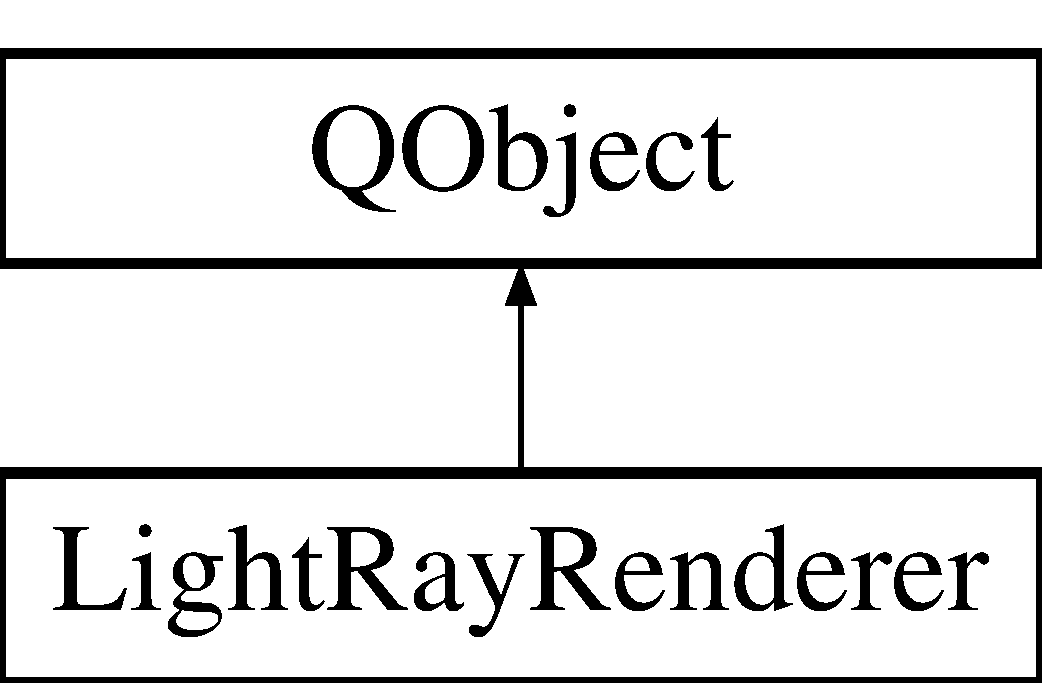
\includegraphics[height=2.000000cm]{class_light_ray_renderer}
\end{center}
\end{figure}
\subsection*{Public Member Functions}
\begin{DoxyCompactItemize}
\item 
\hypertarget{class_light_ray_renderer_a081e83e5e16a36faec002878052aab04}{}{\bfseries Light\+Ray\+Renderer} (Q\+Object $\ast$parent=0)\label{class_light_ray_renderer_a081e83e5e16a36faec002878052aab04}

\item 
\hypertarget{class_light_ray_renderer_a0e481c5c466f2423e06adfde398f6a28}{}void {\bfseries add\+Light\+Ray} (const \hyperlink{class_light_ray}{Light\+Ray} \&light\+Ray)\label{class_light_ray_renderer_a0e481c5c466f2423e06adfde398f6a28}

\item 
\hypertarget{class_light_ray_renderer_a3270c30bd4f5eba01e543bb196c501ed}{}virtual void {\bfseries paint} (Q\+Open\+G\+L\+Functions \&gl, const Q\+Matrix4x4 \&view\+Projection, Q\+Open\+G\+L\+Shader\+Program \&shader\+Program)\label{class_light_ray_renderer_a3270c30bd4f5eba01e543bb196c501ed}

\end{DoxyCompactItemize}
\subsection*{Protected Member Functions}
\begin{DoxyCompactItemize}
\item 
\hypertarget{class_light_ray_renderer_a26948ed2a22fac94af809d293cecf135}{}void {\bfseries update\+Static\+V\+B\+O} ()\label{class_light_ray_renderer_a26948ed2a22fac94af809d293cecf135}

\item 
\hypertarget{class_light_ray_renderer_aa60b1a942ae0b926f4126836dc19ea21}{}void {\bfseries update\+Dynamic\+V\+B\+O} ()\label{class_light_ray_renderer_aa60b1a942ae0b926f4126836dc19ea21}

\item 
\hypertarget{class_light_ray_renderer_a6f7367b897a492fd021ea2ae43053cef}{}void {\bfseries calculate\+Vertex\+Data\+For} (const \hyperlink{class_light_ray_data}{Light\+Ray\+Data} \&ray\+Data, \hyperlink{class_q_vector}{Q\+Vector}$<$ float $>$ \&vertices, \hyperlink{class_q_vector}{Q\+Vector}$<$ unsigned int $>$ \&indices)\label{class_light_ray_renderer_a6f7367b897a492fd021ea2ae43053cef}

\end{DoxyCompactItemize}
\subsection*{Protected Attributes}
\begin{DoxyCompactItemize}
\item 
\hypertarget{class_light_ray_renderer_a9931d2944cabf289973c862a714fc5fd}{}bool {\bfseries m\+\_\+is\+Static\+V\+B\+O\+Update\+Required}\label{class_light_ray_renderer_a9931d2944cabf289973c862a714fc5fd}

\item 
\hypertarget{class_light_ray_renderer_af21bb4b6a08c84b13753860a0a89b199}{}Q\+Open\+G\+L\+Buffer $\ast$ {\bfseries m\+\_\+static\+Vertex\+Buffer}\label{class_light_ray_renderer_af21bb4b6a08c84b13753860a0a89b199}

\item 
\hypertarget{class_light_ray_renderer_ab78cd6dadbb241b4d8929f5f1b60995a}{}Q\+Open\+G\+L\+Buffer $\ast$ {\bfseries m\+\_\+static\+Index\+Buffer}\label{class_light_ray_renderer_ab78cd6dadbb241b4d8929f5f1b60995a}

\item 
\hypertarget{class_light_ray_renderer_ae8c0c8b69c3dda2e8e535f3c7da7543f}{}Q\+Open\+G\+L\+Buffer $\ast$ {\bfseries m\+\_\+dynamic\+Vertex\+Buffer}\label{class_light_ray_renderer_ae8c0c8b69c3dda2e8e535f3c7da7543f}

\item 
\hypertarget{class_light_ray_renderer_afe1bab9c62f8e91c45df4680f1f878a9}{}Q\+Open\+G\+L\+Buffer $\ast$ {\bfseries m\+\_\+dynamic\+Index\+Buffer}\label{class_light_ray_renderer_afe1bab9c62f8e91c45df4680f1f878a9}

\item 
\hypertarget{class_light_ray_renderer_a994b774bb19f4d310593b18a40a41af7}{}\hyperlink{class_q_vector}{Q\+Vector}$<$ \hyperlink{class_light_ray_data}{Light\+Ray\+Data} $>$ $\ast$ {\bfseries m\+\_\+dynamic\+Rays}\label{class_light_ray_renderer_a994b774bb19f4d310593b18a40a41af7}

\item 
\hypertarget{class_light_ray_renderer_a6524c19725083f59fe41616998dcf111}{}\hyperlink{class_q_set}{Q\+Set}$<$ \hyperlink{class_light_ray_data}{Light\+Ray\+Data} $>$ $\ast$ {\bfseries m\+\_\+static\+Rays}\label{class_light_ray_renderer_a6524c19725083f59fe41616998dcf111}

\end{DoxyCompactItemize}


The documentation for this class was generated from the following files\+:\begin{DoxyCompactItemize}
\item 
gem\+Illuminator/lightrayrenderer.\+h\item 
gem\+Illuminator/lightrayrenderer.\+cpp\end{DoxyCompactItemize}

\hypertarget{class_navigation}{}\section{Navigation Class Reference}
\label{class_navigation}\index{Navigation@{Navigation}}


The \hyperlink{class_navigation}{Navigation} class provides an interface for all navigation techniques.  The navigation takes euler angles in coordinate system based on current view and translate them into quaternions describing the changes in our world.  




{\ttfamily \#include $<$navigation.\+h$>$}

Inheritance diagram for Navigation\+:\begin{figure}[H]
\begin{center}
\leavevmode
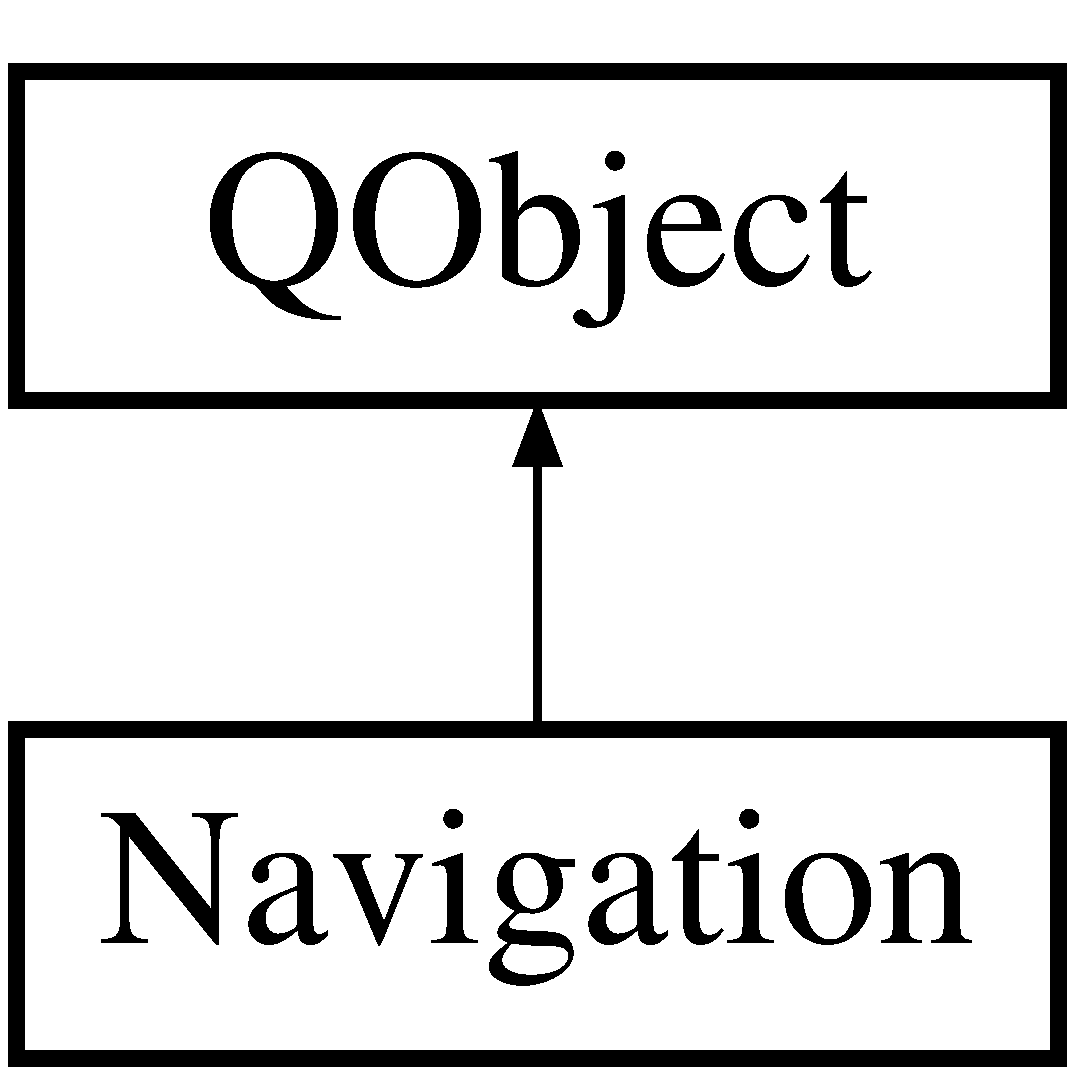
\includegraphics[height=2.000000cm]{class_navigation}
\end{center}
\end{figure}
\subsection*{Signals}
\begin{DoxyCompactItemize}
\item 
void \hyperlink{class_navigation_a46da025077023f9c225d3f5dfe870324}{euler\+Rotation\+Changed} (const Q\+Vector3\+D \&\hyperlink{class_navigation_a264e178e874b62aec38c9986a234d044}{rotation})
\item 
void \hyperlink{class_navigation_ac54fe5d8be2858c2988a9f5158d2d58e}{rotation\+Changed} (const Q\+Quaternion \&\hyperlink{class_navigation_a264e178e874b62aec38c9986a234d044}{rotation})
\item 
void \hyperlink{class_navigation_aa8de8f9227de65da000d1ce730821bab}{world\+Space\+Rotation\+Changed} (const Q\+Quaternion \&\hyperlink{class_navigation_a264e178e874b62aec38c9986a234d044}{rotation})
\end{DoxyCompactItemize}
\subsection*{Public Member Functions}
\begin{DoxyCompactItemize}
\item 
\hyperlink{class_navigation_a9848e09ca6fab3590ffdb0e1c188f31d}{Navigation} (Q\+Object $\ast$parent=0)
\item 
virtual \hyperlink{class_navigation_addd4022d716df48f4e55a1db69361ba7}{$\sim$\+Navigation} ()
\item 
Q\+Quaternion \hyperlink{class_navigation_a264e178e874b62aec38c9986a234d044}{rotation} () const 
\item 
Q\+Quaternion \hyperlink{class_navigation_adedf1fd31c40b2ba7461f67387bbb00c}{world\+Space\+Rotation} () const 
\item 
void \hyperlink{class_navigation_a945e0c9bd30f3c66da040f3242864027}{set\+Camera} (\hyperlink{class_camera}{Camera} $\ast$camera)
\item 
const Q\+Vector3\+D \& \hyperlink{class_navigation_ac756f0b773b771556505a8f20a5f2cf1}{euler\+Rotation} () const 
\item 
void \hyperlink{class_navigation_a4d9b8c12ac091a1db0c3b89f0e36cedd}{set\+Euler\+Rotation} (const Q\+Vector3\+D \&angles)
\end{DoxyCompactItemize}
\subsection*{Protected Member Functions}
\begin{DoxyCompactItemize}
\item 
Q\+Quaternion \hyperlink{class_navigation_a210a31fd6fc626468793b4dbeefcaf2c}{from\+Euler\+Angle\+Quaternions} (const Q\+Quaternion \&x, const Q\+Quaternion \&y, const Q\+Quaternion \&z) const 
\end{DoxyCompactItemize}
\subsection*{Protected Attributes}
\begin{DoxyCompactItemize}
\item 
\hyperlink{class_camera}{Camera} $\ast$ \hyperlink{class_navigation_a76a3e3ea5f8d81a19b22806eb3536302}{m\+\_\+camera}
\item 
Q\+Vector3\+D $\ast$ \hyperlink{class_navigation_a6b056244895c4250c697f6b924874b05}{m\+\_\+euler\+Rotation}
\end{DoxyCompactItemize}
\subsection*{Properties}
\begin{DoxyCompactItemize}
\item 
const Q\+Vector3\+D \hyperlink{class_navigation_a34c974ef7c98cf9853a4ac62ab42ac2f}{euler\+Rotation}
\end{DoxyCompactItemize}


\subsection{Detailed Description}
The \hyperlink{class_navigation}{Navigation} class provides an interface for all navigation techniques.  The navigation takes euler angles in coordinate system based on current view and translate them into quaternions describing the changes in our world. 

\subsection{Constructor \& Destructor Documentation}
\hypertarget{class_navigation_a9848e09ca6fab3590ffdb0e1c188f31d}{}\index{Navigation@{Navigation}!Navigation@{Navigation}}
\index{Navigation@{Navigation}!Navigation@{Navigation}}
\subsubsection[{Navigation}]{\setlength{\rightskip}{0pt plus 5cm}Navigation\+::\+Navigation (
\begin{DoxyParamCaption}
\item[{Q\+Object $\ast$}]{parent = {\ttfamily 0}}
\end{DoxyParamCaption}
)\hspace{0.3cm}{\ttfamily [explicit]}}\label{class_navigation_a9848e09ca6fab3590ffdb0e1c188f31d}
\hypertarget{class_navigation_addd4022d716df48f4e55a1db69361ba7}{}\index{Navigation@{Navigation}!````~Navigation@{$\sim$\+Navigation}}
\index{````~Navigation@{$\sim$\+Navigation}!Navigation@{Navigation}}
\subsubsection[{$\sim$\+Navigation}]{\setlength{\rightskip}{0pt plus 5cm}Navigation\+::$\sim$\+Navigation (
\begin{DoxyParamCaption}
{}
\end{DoxyParamCaption}
)\hspace{0.3cm}{\ttfamily [virtual]}}\label{class_navigation_addd4022d716df48f4e55a1db69361ba7}


\subsection{Member Function Documentation}
\hypertarget{class_navigation_ac756f0b773b771556505a8f20a5f2cf1}{}\index{Navigation@{Navigation}!euler\+Rotation@{euler\+Rotation}}
\index{euler\+Rotation@{euler\+Rotation}!Navigation@{Navigation}}
\subsubsection[{euler\+Rotation}]{\setlength{\rightskip}{0pt plus 5cm}const Q\+Vector3\+D\& Navigation\+::euler\+Rotation (
\begin{DoxyParamCaption}
{}
\end{DoxyParamCaption}
) const}\label{class_navigation_ac756f0b773b771556505a8f20a5f2cf1}
\hypertarget{class_navigation_a46da025077023f9c225d3f5dfe870324}{}\index{Navigation@{Navigation}!euler\+Rotation\+Changed@{euler\+Rotation\+Changed}}
\index{euler\+Rotation\+Changed@{euler\+Rotation\+Changed}!Navigation@{Navigation}}
\subsubsection[{euler\+Rotation\+Changed}]{\setlength{\rightskip}{0pt plus 5cm}void Navigation\+::euler\+Rotation\+Changed (
\begin{DoxyParamCaption}
\item[{const Q\+Vector3\+D \&}]{rotation}
\end{DoxyParamCaption}
)\hspace{0.3cm}{\ttfamily [signal]}}\label{class_navigation_a46da025077023f9c225d3f5dfe870324}
\hypertarget{class_navigation_a210a31fd6fc626468793b4dbeefcaf2c}{}\index{Navigation@{Navigation}!from\+Euler\+Angle\+Quaternions@{from\+Euler\+Angle\+Quaternions}}
\index{from\+Euler\+Angle\+Quaternions@{from\+Euler\+Angle\+Quaternions}!Navigation@{Navigation}}
\subsubsection[{from\+Euler\+Angle\+Quaternions}]{\setlength{\rightskip}{0pt plus 5cm}Q\+Quaternion Navigation\+::from\+Euler\+Angle\+Quaternions (
\begin{DoxyParamCaption}
\item[{const Q\+Quaternion \&}]{x, }
\item[{const Q\+Quaternion \&}]{y, }
\item[{const Q\+Quaternion \&}]{z}
\end{DoxyParamCaption}
) const\hspace{0.3cm}{\ttfamily [protected]}}\label{class_navigation_a210a31fd6fc626468793b4dbeefcaf2c}
\hypertarget{class_navigation_a264e178e874b62aec38c9986a234d044}{}\index{Navigation@{Navigation}!rotation@{rotation}}
\index{rotation@{rotation}!Navigation@{Navigation}}
\subsubsection[{rotation}]{\setlength{\rightskip}{0pt plus 5cm}Q\+Quaternion Navigation\+::rotation (
\begin{DoxyParamCaption}
{}
\end{DoxyParamCaption}
) const}\label{class_navigation_a264e178e874b62aec38c9986a234d044}
\hypertarget{class_navigation_ac54fe5d8be2858c2988a9f5158d2d58e}{}\index{Navigation@{Navigation}!rotation\+Changed@{rotation\+Changed}}
\index{rotation\+Changed@{rotation\+Changed}!Navigation@{Navigation}}
\subsubsection[{rotation\+Changed}]{\setlength{\rightskip}{0pt plus 5cm}void Navigation\+::rotation\+Changed (
\begin{DoxyParamCaption}
\item[{const Q\+Quaternion \&}]{rotation}
\end{DoxyParamCaption}
)\hspace{0.3cm}{\ttfamily [signal]}}\label{class_navigation_ac54fe5d8be2858c2988a9f5158d2d58e}
\hypertarget{class_navigation_a945e0c9bd30f3c66da040f3242864027}{}\index{Navigation@{Navigation}!set\+Camera@{set\+Camera}}
\index{set\+Camera@{set\+Camera}!Navigation@{Navigation}}
\subsubsection[{set\+Camera}]{\setlength{\rightskip}{0pt plus 5cm}void Navigation\+::set\+Camera (
\begin{DoxyParamCaption}
\item[{{\bf Camera} $\ast$}]{camera}
\end{DoxyParamCaption}
)}\label{class_navigation_a945e0c9bd30f3c66da040f3242864027}
\hypertarget{class_navigation_a4d9b8c12ac091a1db0c3b89f0e36cedd}{}\index{Navigation@{Navigation}!set\+Euler\+Rotation@{set\+Euler\+Rotation}}
\index{set\+Euler\+Rotation@{set\+Euler\+Rotation}!Navigation@{Navigation}}
\subsubsection[{set\+Euler\+Rotation}]{\setlength{\rightskip}{0pt plus 5cm}void Navigation\+::set\+Euler\+Rotation (
\begin{DoxyParamCaption}
\item[{const Q\+Vector3\+D \&}]{angles}
\end{DoxyParamCaption}
)}\label{class_navigation_a4d9b8c12ac091a1db0c3b89f0e36cedd}
\hypertarget{class_navigation_adedf1fd31c40b2ba7461f67387bbb00c}{}\index{Navigation@{Navigation}!world\+Space\+Rotation@{world\+Space\+Rotation}}
\index{world\+Space\+Rotation@{world\+Space\+Rotation}!Navigation@{Navigation}}
\subsubsection[{world\+Space\+Rotation}]{\setlength{\rightskip}{0pt plus 5cm}Q\+Quaternion Navigation\+::world\+Space\+Rotation (
\begin{DoxyParamCaption}
{}
\end{DoxyParamCaption}
) const}\label{class_navigation_adedf1fd31c40b2ba7461f67387bbb00c}
\hypertarget{class_navigation_aa8de8f9227de65da000d1ce730821bab}{}\index{Navigation@{Navigation}!world\+Space\+Rotation\+Changed@{world\+Space\+Rotation\+Changed}}
\index{world\+Space\+Rotation\+Changed@{world\+Space\+Rotation\+Changed}!Navigation@{Navigation}}
\subsubsection[{world\+Space\+Rotation\+Changed}]{\setlength{\rightskip}{0pt plus 5cm}void Navigation\+::world\+Space\+Rotation\+Changed (
\begin{DoxyParamCaption}
\item[{const Q\+Quaternion \&}]{rotation}
\end{DoxyParamCaption}
)\hspace{0.3cm}{\ttfamily [signal]}}\label{class_navigation_aa8de8f9227de65da000d1ce730821bab}


\subsection{Member Data Documentation}
\hypertarget{class_navigation_a76a3e3ea5f8d81a19b22806eb3536302}{}\index{Navigation@{Navigation}!m\+\_\+camera@{m\+\_\+camera}}
\index{m\+\_\+camera@{m\+\_\+camera}!Navigation@{Navigation}}
\subsubsection[{m\+\_\+camera}]{\setlength{\rightskip}{0pt plus 5cm}{\bf Camera}$\ast$ Navigation\+::m\+\_\+camera\hspace{0.3cm}{\ttfamily [protected]}}\label{class_navigation_a76a3e3ea5f8d81a19b22806eb3536302}
\hypertarget{class_navigation_a6b056244895c4250c697f6b924874b05}{}\index{Navigation@{Navigation}!m\+\_\+euler\+Rotation@{m\+\_\+euler\+Rotation}}
\index{m\+\_\+euler\+Rotation@{m\+\_\+euler\+Rotation}!Navigation@{Navigation}}
\subsubsection[{m\+\_\+euler\+Rotation}]{\setlength{\rightskip}{0pt plus 5cm}Q\+Vector3\+D$\ast$ Navigation\+::m\+\_\+euler\+Rotation\hspace{0.3cm}{\ttfamily [protected]}}\label{class_navigation_a6b056244895c4250c697f6b924874b05}


\subsection{Property Documentation}
\hypertarget{class_navigation_a34c974ef7c98cf9853a4ac62ab42ac2f}{}\index{Navigation@{Navigation}!euler\+Rotation@{euler\+Rotation}}
\index{euler\+Rotation@{euler\+Rotation}!Navigation@{Navigation}}
\subsubsection[{euler\+Rotation}]{\setlength{\rightskip}{0pt plus 5cm}const Q\+Vector3\+D \& Navigation\+::euler\+Rotation\hspace{0.3cm}{\ttfamily [read]}, {\ttfamily [write]}}\label{class_navigation_a34c974ef7c98cf9853a4ac62ab42ac2f}


The documentation for this class was generated from the following files\+:\begin{DoxyCompactItemize}
\item 
Game-\/\+Programming-\/\+W\+S2014/gem\+Illuminator/\hyperlink{navigation_8h}{navigation.\+h}\item 
Game-\/\+Programming-\/\+W\+S2014/gem\+Illuminator/\hyperlink{navigation_8cpp}{navigation.\+cpp}\end{DoxyCompactItemize}

\hypertarget{class_painter}{}\section{Painter Class Reference}
\label{class_painter}\index{Painter@{Painter}}


The \hyperlink{class_painter}{Painter} class  Includes the rendering process, thus creates the whole picture. The \hyperlink{class_painter}{Painter} will be used by Q\+M\+L within rendering thread.  




{\ttfamily \#include $<$painter.\+h$>$}

Inheritance diagram for Painter\+:\begin{figure}[H]
\begin{center}
\leavevmode
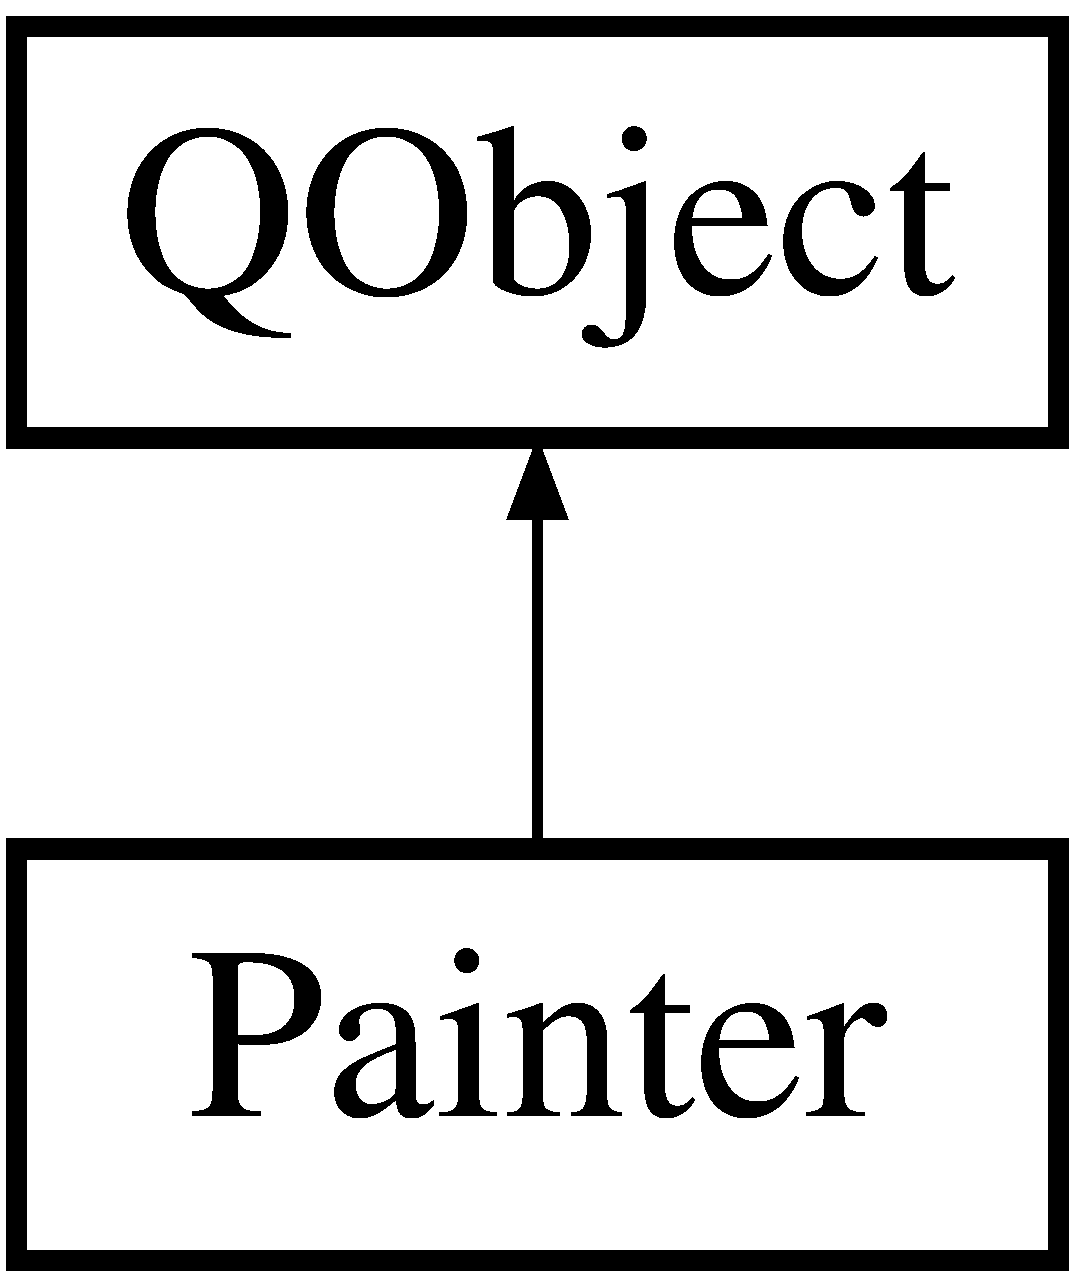
\includegraphics[height=2.000000cm]{class_painter}
\end{center}
\end{figure}
\subsection*{Public Slots}
\begin{DoxyCompactItemize}
\item 
void \hyperlink{class_painter_a5b9b4ed8aebaebeb2f6483e350445fbc}{paint} ()
\begin{DoxyCompactList}\small\item\em Starts rendering and paints the whole picture. \end{DoxyCompactList}\end{DoxyCompactItemize}
\subsection*{Signals}
\begin{DoxyCompactItemize}
\item 
void \hyperlink{class_painter_a171dd523e7ba423b8da554a062168e94}{initialize\+Done} ()
\begin{DoxyCompactList}\small\item\em This signal is emitted if initialization of all required ressources for current scene are initalized.  The signal is everytime emitted if previous scene was deleted and a new scene was synchronized. \end{DoxyCompactList}\end{DoxyCompactItemize}
\subsection*{Public Member Functions}
\begin{DoxyCompactItemize}
\item 
\hyperlink{class_painter_ae9520672fc113fc60cf942ba3d13a46e}{Painter} (\hyperlink{class_painter_q_m_l}{Painter\+Q\+M\+L} $\ast$painter, Q\+Object $\ast$parent=0)
\begin{DoxyCompactList}\small\item\em Constructor of \hyperlink{class_painter}{Painter}. \end{DoxyCompactList}\item 
virtual \hyperlink{class_painter_a6db88212368910da3385fa9e5fa97174}{$\sim$\+Painter} ()
\begin{DoxyCompactList}\small\item\em Destrutor. Will delete all rendering related classes and ressources. \end{DoxyCompactList}\item 
void \hyperlink{class_painter_a3af62665915b5f5380e7009c18862e7e}{update\+Env\+Map} ()
\begin{DoxyCompactList}\small\item\em Updates enviorment map using config file. \end{DoxyCompactList}\item 
bool \hyperlink{class_painter_addfa0fd4dd943d27c67b62dfc9ab3a0b}{is\+Active} () const 
\begin{DoxyCompactList}\small\item\em Check if \hyperlink{class_painter}{Painter} is active. Active means the painter is rendering. \end{DoxyCompactList}\item 
void \hyperlink{class_painter_a7dd43be8d3e1eab98035fcc23316bd1a}{set\+Active} (bool active)
\begin{DoxyCompactList}\small\item\em Set Active state. If active is true the painter renders the picture. \end{DoxyCompactList}\item 
void \hyperlink{class_painter_a37014617684597b602522d3de20f8f41}{clear\+Scene} ()
\begin{DoxyCompactList}\small\item\em Clears the scene and removes all not anymore required ressources. \end{DoxyCompactList}\item 
void \hyperlink{class_painter_a0c7f2b5b2bc7fa8fdfac559cc9b1401d}{synchronize\+Scene} (\hyperlink{class_scene}{Scene} $\ast$scene)
\begin{DoxyCompactList}\small\item\em \hyperlink{class_painter}{Painter} copies all needed information of scene into own thread. \end{DoxyCompactList}\end{DoxyCompactItemize}
\subsection*{Protected Slots}
\begin{DoxyCompactItemize}
\item 
void \hyperlink{class_painter_ab5dbc13d3e46ee83c4f819a5ae74206e}{handle\+Initialize\+Done} ()
\end{DoxyCompactItemize}
\subsection*{Protected Member Functions}
\begin{DoxyCompactItemize}
\item 
void \hyperlink{class_painter_a12f9623c2acf87eced6e141e7638804e}{initialize} ()
\begin{DoxyCompactList}\small\item\em Initializes all required ressources, that are direct members of painter (scene independant ressources). This method is executed within first paint. \end{DoxyCompactList}\item 
void \hyperlink{class_painter_ad7db952528a1d7745dbf083ee1431f50}{initialize\+F\+B\+Os} ()
\item 
void \hyperlink{class_painter_a4fee3b94c00da17f851b52cc8d60ff72}{initialize\+Shader\+Programs} ()
\item 
void \hyperlink{class_painter_a5fee5d930d347b38fe1aa565e3264d3c}{render\+Light\+Rays} (const \hyperlink{class_camera}{Camera} \&camera)
\item 
void \hyperlink{class_painter_a8cbffb0c2d28dd1558716136c99a079f}{render\+Scene} (const \hyperlink{class_camera}{Camera} \&camera)
\end{DoxyCompactItemize}
\subsection*{Protected Attributes}
\begin{DoxyCompactItemize}
\item 
bool \hyperlink{class_painter_a9b476c949ca4b2af7b1653c7106b659b}{m\+\_\+active}
\item 
\hyperlink{class_environment_map}{Environment\+Map} $\ast$ \hyperlink{class_painter_acb7b623817cf6865168bb74d3823897f}{m\+\_\+env\+Map}
\item 
Q\+Open\+G\+L\+Functions $\ast$ \hyperlink{class_painter_a8aa44a5f1477d570ee10d3dacae09f08}{m\+\_\+gl}
\item 
bool \hyperlink{class_painter_a0adcfafb8172b4f76561e2c951b1090b}{m\+\_\+initialized}
\item 
\hyperlink{class_blur_effect}{Blur\+Effect} $\ast$ \hyperlink{class_painter_a951961fa0e012d87500b9775f9dcb19a}{m\+\_\+blur\+Effect\+Scene}
\item 
int \hyperlink{class_painter_a9a58327bf0fd8004e11e97c4415caa62}{m\+\_\+blur\+Viewport\+Ratio\+Scene}
\item 
uint \hyperlink{class_painter_a265ca037babf5497830eda6f42b6aeef}{m\+\_\+glow\+Scene\+F\+B\+O}
\item 
uint \hyperlink{class_painter_af165f6cb73abce18d3c48e4cbba39058}{m\+\_\+glow\+Scene\+Depth\+R\+B}
\item 
uint \hyperlink{class_painter_ab0b0d6b22e49da1a22d3e3114efc6f56}{m\+\_\+glow\+Scene\+Texture}
\item 
\hyperlink{class_blur_effect}{Blur\+Effect} $\ast$ \hyperlink{class_painter_a8960c588485d1ccdb7d4306236e187af}{m\+\_\+blur\+Effect\+Preview\+Scene}
\item 
int \hyperlink{class_painter_ab898af5b9784a08a86a93d9d9f3e6de6}{m\+\_\+blur\+Viewport\+Ratio\+Preview\+Scene}
\item 
uint \hyperlink{class_painter_a68a674089abe95f55b48e12fef4e3a8f}{m\+\_\+glow\+Preview\+Scene\+F\+B\+O}
\item 
uint \hyperlink{class_painter_ae7d26057c7ce98d20f8e11242f9b8d23}{m\+\_\+glow\+Preview\+Scene\+Depth\+R\+B}
\item 
uint \hyperlink{class_painter_a642492c18262a53f20c0824bd70e7526}{m\+\_\+glow\+Preview\+Scene\+Texture}
\item 
uint \hyperlink{class_painter_adb6ae15aabf53d3f2c9108a8db0cbbb5}{m\+\_\+preview\+Scene\+F\+B\+O}
\item 
uint \hyperlink{class_painter_ad4fb3338a366abb5592996572afa070d}{m\+\_\+preview\+Scene\+Depth\+R\+B}
\item 
uint \hyperlink{class_painter_aff56d277a464801c66a7f7414ef86733}{m\+\_\+preview\+Scene\+Texture}
\item 
\hyperlink{class_painter_q_m_l}{Painter\+Q\+M\+L} $\ast$ \hyperlink{class_painter_af2774293bfaf6f654cb01e504937abb8}{m\+\_\+painter\+Q\+M\+L}
\item 
\hyperlink{class_screen_aligned_quad}{Screen\+Aligned\+Quad} $\ast$ \hyperlink{class_painter_a50f7fad2d44554f0be878a96afacfa44}{m\+\_\+quad}
\item 
\hyperlink{class_cube_map}{Cube\+Map} $\ast$ \hyperlink{class_painter_a9f99a5ccb9b1b645281b1439cbf416e1}{m\+\_\+rainbow\+Map}
\item 
\hyperlink{class_cube_map}{Cube\+Map} $\ast$ \hyperlink{class_painter_abd540fa99df6acea8eb32c3bcfb81773}{m\+\_\+gem\+Structure\+Map}
\item 
uint \hyperlink{class_painter_a4df95c88604785d7eecaf1474df67629}{m\+\_\+scene\+F\+B\+O}
\item 
uint \hyperlink{class_painter_a92db0cde0f42dd82569e85785850c283}{m\+\_\+scene\+Depth\+R\+B}
\item 
uint \hyperlink{class_painter_af82c25060227ea6ec91ae60f0753c593}{m\+\_\+scene\+Texture}
\item 
\hyperlink{class_q_hash}{Q\+Hash}$<$ \hyperlink{shaderprograms_8h_ada89718f8d394b2cc093eb9770c554ff}{Shader\+Programs}, Q\+Open\+G\+L\+Shader\+Program $\ast$ $>$ $\ast$ \hyperlink{class_painter_a30655a30ba8f540f0e28b976b97d126f}{m\+\_\+shader\+Programs}
\item 
Q\+Size $\ast$ \hyperlink{class_painter_aff5d274eb90d7a94565effe5bd5d03f7}{m\+\_\+used\+Viewport}
\item 
int \hyperlink{class_painter_a1a3de21931e9796db399252b7336169c}{m\+\_\+counter}
\item 
int \hyperlink{class_painter_aedfda3eb1a37f4f121291c558786492a}{m\+\_\+old\+Elapsed}
\item 
Q\+Time $\ast$ \hyperlink{class_painter_ab6976ab19027866bbb01e9a1504aa5c9}{m\+\_\+time}
\item 
\hyperlink{class_scene_renderer}{Scene\+Renderer} $\ast$ \hyperlink{class_painter_a574ba64fd2af1d8c64d2c293d4811fc2}{m\+\_\+scene\+Renderer}
\item 
\hyperlink{class_camera}{Camera} $\ast$ \hyperlink{class_painter_a05558ea7a2f818641e0506d01d518010}{m\+\_\+camera}
\item 
\hyperlink{class_camera}{Camera} $\ast$ \hyperlink{class_painter_a237399ac0b5da625eb19de1ae3c0a236}{m\+\_\+preview\+Camera}
\end{DoxyCompactItemize}


\subsection{Detailed Description}
The \hyperlink{class_painter}{Painter} class  Includes the rendering process, thus creates the whole picture. The \hyperlink{class_painter}{Painter} will be used by Q\+M\+L within rendering thread. 

\subsection{Constructor \& Destructor Documentation}
\hypertarget{class_painter_ae9520672fc113fc60cf942ba3d13a46e}{}\index{Painter@{Painter}!Painter@{Painter}}
\index{Painter@{Painter}!Painter@{Painter}}
\subsubsection[{Painter}]{\setlength{\rightskip}{0pt plus 5cm}Painter\+::\+Painter (
\begin{DoxyParamCaption}
\item[{{\bf Painter\+Q\+M\+L} $\ast$}]{painter, }
\item[{Q\+Object $\ast$}]{parent = {\ttfamily 0}}
\end{DoxyParamCaption}
)\hspace{0.3cm}{\ttfamily [explicit]}}\label{class_painter_ae9520672fc113fc60cf942ba3d13a46e}


Constructor of \hyperlink{class_painter}{Painter}. 


\begin{DoxyParams}{Parameters}
{\em painter} & Corresponding Q\+M\+L-\/\+Painter. Will be informed about finished rendering. \\
\hline
{\em parent} & Q\+Object-\/parent \\
\hline
\end{DoxyParams}
\hypertarget{class_painter_a6db88212368910da3385fa9e5fa97174}{}\index{Painter@{Painter}!````~Painter@{$\sim$\+Painter}}
\index{````~Painter@{$\sim$\+Painter}!Painter@{Painter}}
\subsubsection[{$\sim$\+Painter}]{\setlength{\rightskip}{0pt plus 5cm}Painter\+::$\sim$\+Painter (
\begin{DoxyParamCaption}
{}
\end{DoxyParamCaption}
)\hspace{0.3cm}{\ttfamily [virtual]}}\label{class_painter_a6db88212368910da3385fa9e5fa97174}


Destrutor. Will delete all rendering related classes and ressources. 



\subsection{Member Function Documentation}
\hypertarget{class_painter_a37014617684597b602522d3de20f8f41}{}\index{Painter@{Painter}!clear\+Scene@{clear\+Scene}}
\index{clear\+Scene@{clear\+Scene}!Painter@{Painter}}
\subsubsection[{clear\+Scene}]{\setlength{\rightskip}{0pt plus 5cm}void Painter\+::clear\+Scene (
\begin{DoxyParamCaption}
{}
\end{DoxyParamCaption}
)}\label{class_painter_a37014617684597b602522d3de20f8f41}


Clears the scene and removes all not anymore required ressources. 

\hypertarget{class_painter_ab5dbc13d3e46ee83c4f819a5ae74206e}{}\index{Painter@{Painter}!handle\+Initialize\+Done@{handle\+Initialize\+Done}}
\index{handle\+Initialize\+Done@{handle\+Initialize\+Done}!Painter@{Painter}}
\subsubsection[{handle\+Initialize\+Done}]{\setlength{\rightskip}{0pt plus 5cm}void Painter\+::handle\+Initialize\+Done (
\begin{DoxyParamCaption}
{}
\end{DoxyParamCaption}
)\hspace{0.3cm}{\ttfamily [protected]}, {\ttfamily [slot]}}\label{class_painter_ab5dbc13d3e46ee83c4f819a5ae74206e}
\hypertarget{class_painter_a12f9623c2acf87eced6e141e7638804e}{}\index{Painter@{Painter}!initialize@{initialize}}
\index{initialize@{initialize}!Painter@{Painter}}
\subsubsection[{initialize}]{\setlength{\rightskip}{0pt plus 5cm}void Painter\+::initialize (
\begin{DoxyParamCaption}
{}
\end{DoxyParamCaption}
)\hspace{0.3cm}{\ttfamily [protected]}}\label{class_painter_a12f9623c2acf87eced6e141e7638804e}


Initializes all required ressources, that are direct members of painter (scene independant ressources). This method is executed within first paint. 

\hypertarget{class_painter_a171dd523e7ba423b8da554a062168e94}{}\index{Painter@{Painter}!initialize\+Done@{initialize\+Done}}
\index{initialize\+Done@{initialize\+Done}!Painter@{Painter}}
\subsubsection[{initialize\+Done}]{\setlength{\rightskip}{0pt plus 5cm}void Painter\+::initialize\+Done (
\begin{DoxyParamCaption}
{}
\end{DoxyParamCaption}
)\hspace{0.3cm}{\ttfamily [signal]}}\label{class_painter_a171dd523e7ba423b8da554a062168e94}


This signal is emitted if initialization of all required ressources for current scene are initalized.  The signal is everytime emitted if previous scene was deleted and a new scene was synchronized. 

\hypertarget{class_painter_ad7db952528a1d7745dbf083ee1431f50}{}\index{Painter@{Painter}!initialize\+F\+B\+Os@{initialize\+F\+B\+Os}}
\index{initialize\+F\+B\+Os@{initialize\+F\+B\+Os}!Painter@{Painter}}
\subsubsection[{initialize\+F\+B\+Os}]{\setlength{\rightskip}{0pt plus 5cm}void Painter\+::initialize\+F\+B\+Os (
\begin{DoxyParamCaption}
{}
\end{DoxyParamCaption}
)\hspace{0.3cm}{\ttfamily [protected]}}\label{class_painter_ad7db952528a1d7745dbf083ee1431f50}
\hypertarget{class_painter_a4fee3b94c00da17f851b52cc8d60ff72}{}\index{Painter@{Painter}!initialize\+Shader\+Programs@{initialize\+Shader\+Programs}}
\index{initialize\+Shader\+Programs@{initialize\+Shader\+Programs}!Painter@{Painter}}
\subsubsection[{initialize\+Shader\+Programs}]{\setlength{\rightskip}{0pt plus 5cm}void Painter\+::initialize\+Shader\+Programs (
\begin{DoxyParamCaption}
{}
\end{DoxyParamCaption}
)\hspace{0.3cm}{\ttfamily [protected]}}\label{class_painter_a4fee3b94c00da17f851b52cc8d60ff72}
\hypertarget{class_painter_addfa0fd4dd943d27c67b62dfc9ab3a0b}{}\index{Painter@{Painter}!is\+Active@{is\+Active}}
\index{is\+Active@{is\+Active}!Painter@{Painter}}
\subsubsection[{is\+Active}]{\setlength{\rightskip}{0pt plus 5cm}bool Painter\+::is\+Active (
\begin{DoxyParamCaption}
{}
\end{DoxyParamCaption}
) const}\label{class_painter_addfa0fd4dd943d27c67b62dfc9ab3a0b}


Check if \hyperlink{class_painter}{Painter} is active. Active means the painter is rendering. 

\begin{DoxyReturn}{Returns}
Active state of painter. 
\end{DoxyReturn}
\hypertarget{class_painter_a5b9b4ed8aebaebeb2f6483e350445fbc}{}\index{Painter@{Painter}!paint@{paint}}
\index{paint@{paint}!Painter@{Painter}}
\subsubsection[{paint}]{\setlength{\rightskip}{0pt plus 5cm}void Painter\+::paint (
\begin{DoxyParamCaption}
{}
\end{DoxyParamCaption}
)\hspace{0.3cm}{\ttfamily [slot]}}\label{class_painter_a5b9b4ed8aebaebeb2f6483e350445fbc}


Starts rendering and paints the whole picture. 

\hypertarget{class_painter_a5fee5d930d347b38fe1aa565e3264d3c}{}\index{Painter@{Painter}!render\+Light\+Rays@{render\+Light\+Rays}}
\index{render\+Light\+Rays@{render\+Light\+Rays}!Painter@{Painter}}
\subsubsection[{render\+Light\+Rays}]{\setlength{\rightskip}{0pt plus 5cm}void Painter\+::render\+Light\+Rays (
\begin{DoxyParamCaption}
\item[{const {\bf Camera} \&}]{camera}
\end{DoxyParamCaption}
)\hspace{0.3cm}{\ttfamily [protected]}}\label{class_painter_a5fee5d930d347b38fe1aa565e3264d3c}
\hypertarget{class_painter_a8cbffb0c2d28dd1558716136c99a079f}{}\index{Painter@{Painter}!render\+Scene@{render\+Scene}}
\index{render\+Scene@{render\+Scene}!Painter@{Painter}}
\subsubsection[{render\+Scene}]{\setlength{\rightskip}{0pt plus 5cm}void Painter\+::render\+Scene (
\begin{DoxyParamCaption}
\item[{const {\bf Camera} \&}]{camera}
\end{DoxyParamCaption}
)\hspace{0.3cm}{\ttfamily [protected]}}\label{class_painter_a8cbffb0c2d28dd1558716136c99a079f}
\hypertarget{class_painter_a7dd43be8d3e1eab98035fcc23316bd1a}{}\index{Painter@{Painter}!set\+Active@{set\+Active}}
\index{set\+Active@{set\+Active}!Painter@{Painter}}
\subsubsection[{set\+Active}]{\setlength{\rightskip}{0pt plus 5cm}void Painter\+::set\+Active (
\begin{DoxyParamCaption}
\item[{bool}]{active}
\end{DoxyParamCaption}
)}\label{class_painter_a7dd43be8d3e1eab98035fcc23316bd1a}


Set Active state. If active is true the painter renders the picture. 


\begin{DoxyParams}{Parameters}
{\em active} & \\
\hline
\end{DoxyParams}
\hypertarget{class_painter_a0c7f2b5b2bc7fa8fdfac559cc9b1401d}{}\index{Painter@{Painter}!synchronize\+Scene@{synchronize\+Scene}}
\index{synchronize\+Scene@{synchronize\+Scene}!Painter@{Painter}}
\subsubsection[{synchronize\+Scene}]{\setlength{\rightskip}{0pt plus 5cm}void Painter\+::synchronize\+Scene (
\begin{DoxyParamCaption}
\item[{{\bf Scene} $\ast$}]{scene}
\end{DoxyParamCaption}
)}\label{class_painter_a0c7f2b5b2bc7fa8fdfac559cc9b1401d}


\hyperlink{class_painter}{Painter} copies all needed information of scene into own thread. 


\begin{DoxyParams}{Parameters}
{\em scene} & The scene that should be synchronized. If nullptr is passed it is like \hyperlink{class_painter_a37014617684597b602522d3de20f8f41}{clear\+Scene()} \\
\hline
\end{DoxyParams}
\hypertarget{class_painter_a3af62665915b5f5380e7009c18862e7e}{}\index{Painter@{Painter}!update\+Env\+Map@{update\+Env\+Map}}
\index{update\+Env\+Map@{update\+Env\+Map}!Painter@{Painter}}
\subsubsection[{update\+Env\+Map}]{\setlength{\rightskip}{0pt plus 5cm}void Painter\+::update\+Env\+Map (
\begin{DoxyParamCaption}
{}
\end{DoxyParamCaption}
)}\label{class_painter_a3af62665915b5f5380e7009c18862e7e}


Updates enviorment map using config file. 



\subsection{Member Data Documentation}
\hypertarget{class_painter_a9b476c949ca4b2af7b1653c7106b659b}{}\index{Painter@{Painter}!m\+\_\+active@{m\+\_\+active}}
\index{m\+\_\+active@{m\+\_\+active}!Painter@{Painter}}
\subsubsection[{m\+\_\+active}]{\setlength{\rightskip}{0pt plus 5cm}bool Painter\+::m\+\_\+active\hspace{0.3cm}{\ttfamily [protected]}}\label{class_painter_a9b476c949ca4b2af7b1653c7106b659b}
\hypertarget{class_painter_a8960c588485d1ccdb7d4306236e187af}{}\index{Painter@{Painter}!m\+\_\+blur\+Effect\+Preview\+Scene@{m\+\_\+blur\+Effect\+Preview\+Scene}}
\index{m\+\_\+blur\+Effect\+Preview\+Scene@{m\+\_\+blur\+Effect\+Preview\+Scene}!Painter@{Painter}}
\subsubsection[{m\+\_\+blur\+Effect\+Preview\+Scene}]{\setlength{\rightskip}{0pt plus 5cm}{\bf Blur\+Effect}$\ast$ Painter\+::m\+\_\+blur\+Effect\+Preview\+Scene\hspace{0.3cm}{\ttfamily [protected]}}\label{class_painter_a8960c588485d1ccdb7d4306236e187af}
\hypertarget{class_painter_a951961fa0e012d87500b9775f9dcb19a}{}\index{Painter@{Painter}!m\+\_\+blur\+Effect\+Scene@{m\+\_\+blur\+Effect\+Scene}}
\index{m\+\_\+blur\+Effect\+Scene@{m\+\_\+blur\+Effect\+Scene}!Painter@{Painter}}
\subsubsection[{m\+\_\+blur\+Effect\+Scene}]{\setlength{\rightskip}{0pt plus 5cm}{\bf Blur\+Effect}$\ast$ Painter\+::m\+\_\+blur\+Effect\+Scene\hspace{0.3cm}{\ttfamily [protected]}}\label{class_painter_a951961fa0e012d87500b9775f9dcb19a}
\hypertarget{class_painter_ab898af5b9784a08a86a93d9d9f3e6de6}{}\index{Painter@{Painter}!m\+\_\+blur\+Viewport\+Ratio\+Preview\+Scene@{m\+\_\+blur\+Viewport\+Ratio\+Preview\+Scene}}
\index{m\+\_\+blur\+Viewport\+Ratio\+Preview\+Scene@{m\+\_\+blur\+Viewport\+Ratio\+Preview\+Scene}!Painter@{Painter}}
\subsubsection[{m\+\_\+blur\+Viewport\+Ratio\+Preview\+Scene}]{\setlength{\rightskip}{0pt plus 5cm}int Painter\+::m\+\_\+blur\+Viewport\+Ratio\+Preview\+Scene\hspace{0.3cm}{\ttfamily [protected]}}\label{class_painter_ab898af5b9784a08a86a93d9d9f3e6de6}
\hypertarget{class_painter_a9a58327bf0fd8004e11e97c4415caa62}{}\index{Painter@{Painter}!m\+\_\+blur\+Viewport\+Ratio\+Scene@{m\+\_\+blur\+Viewport\+Ratio\+Scene}}
\index{m\+\_\+blur\+Viewport\+Ratio\+Scene@{m\+\_\+blur\+Viewport\+Ratio\+Scene}!Painter@{Painter}}
\subsubsection[{m\+\_\+blur\+Viewport\+Ratio\+Scene}]{\setlength{\rightskip}{0pt plus 5cm}int Painter\+::m\+\_\+blur\+Viewport\+Ratio\+Scene\hspace{0.3cm}{\ttfamily [protected]}}\label{class_painter_a9a58327bf0fd8004e11e97c4415caa62}
\hypertarget{class_painter_a05558ea7a2f818641e0506d01d518010}{}\index{Painter@{Painter}!m\+\_\+camera@{m\+\_\+camera}}
\index{m\+\_\+camera@{m\+\_\+camera}!Painter@{Painter}}
\subsubsection[{m\+\_\+camera}]{\setlength{\rightskip}{0pt plus 5cm}{\bf Camera}$\ast$ Painter\+::m\+\_\+camera\hspace{0.3cm}{\ttfamily [protected]}}\label{class_painter_a05558ea7a2f818641e0506d01d518010}
\hypertarget{class_painter_a1a3de21931e9796db399252b7336169c}{}\index{Painter@{Painter}!m\+\_\+counter@{m\+\_\+counter}}
\index{m\+\_\+counter@{m\+\_\+counter}!Painter@{Painter}}
\subsubsection[{m\+\_\+counter}]{\setlength{\rightskip}{0pt plus 5cm}int Painter\+::m\+\_\+counter\hspace{0.3cm}{\ttfamily [protected]}}\label{class_painter_a1a3de21931e9796db399252b7336169c}
\hypertarget{class_painter_acb7b623817cf6865168bb74d3823897f}{}\index{Painter@{Painter}!m\+\_\+env\+Map@{m\+\_\+env\+Map}}
\index{m\+\_\+env\+Map@{m\+\_\+env\+Map}!Painter@{Painter}}
\subsubsection[{m\+\_\+env\+Map}]{\setlength{\rightskip}{0pt plus 5cm}{\bf Environment\+Map}$\ast$ Painter\+::m\+\_\+env\+Map\hspace{0.3cm}{\ttfamily [protected]}}\label{class_painter_acb7b623817cf6865168bb74d3823897f}
\hypertarget{class_painter_abd540fa99df6acea8eb32c3bcfb81773}{}\index{Painter@{Painter}!m\+\_\+gem\+Structure\+Map@{m\+\_\+gem\+Structure\+Map}}
\index{m\+\_\+gem\+Structure\+Map@{m\+\_\+gem\+Structure\+Map}!Painter@{Painter}}
\subsubsection[{m\+\_\+gem\+Structure\+Map}]{\setlength{\rightskip}{0pt plus 5cm}{\bf Cube\+Map}$\ast$ Painter\+::m\+\_\+gem\+Structure\+Map\hspace{0.3cm}{\ttfamily [protected]}}\label{class_painter_abd540fa99df6acea8eb32c3bcfb81773}
\hypertarget{class_painter_a8aa44a5f1477d570ee10d3dacae09f08}{}\index{Painter@{Painter}!m\+\_\+gl@{m\+\_\+gl}}
\index{m\+\_\+gl@{m\+\_\+gl}!Painter@{Painter}}
\subsubsection[{m\+\_\+gl}]{\setlength{\rightskip}{0pt plus 5cm}Q\+Open\+G\+L\+Functions$\ast$ Painter\+::m\+\_\+gl\hspace{0.3cm}{\ttfamily [protected]}}\label{class_painter_a8aa44a5f1477d570ee10d3dacae09f08}
\hypertarget{class_painter_ae7d26057c7ce98d20f8e11242f9b8d23}{}\index{Painter@{Painter}!m\+\_\+glow\+Preview\+Scene\+Depth\+R\+B@{m\+\_\+glow\+Preview\+Scene\+Depth\+R\+B}}
\index{m\+\_\+glow\+Preview\+Scene\+Depth\+R\+B@{m\+\_\+glow\+Preview\+Scene\+Depth\+R\+B}!Painter@{Painter}}
\subsubsection[{m\+\_\+glow\+Preview\+Scene\+Depth\+R\+B}]{\setlength{\rightskip}{0pt plus 5cm}uint Painter\+::m\+\_\+glow\+Preview\+Scene\+Depth\+R\+B\hspace{0.3cm}{\ttfamily [protected]}}\label{class_painter_ae7d26057c7ce98d20f8e11242f9b8d23}
\hypertarget{class_painter_a68a674089abe95f55b48e12fef4e3a8f}{}\index{Painter@{Painter}!m\+\_\+glow\+Preview\+Scene\+F\+B\+O@{m\+\_\+glow\+Preview\+Scene\+F\+B\+O}}
\index{m\+\_\+glow\+Preview\+Scene\+F\+B\+O@{m\+\_\+glow\+Preview\+Scene\+F\+B\+O}!Painter@{Painter}}
\subsubsection[{m\+\_\+glow\+Preview\+Scene\+F\+B\+O}]{\setlength{\rightskip}{0pt plus 5cm}uint Painter\+::m\+\_\+glow\+Preview\+Scene\+F\+B\+O\hspace{0.3cm}{\ttfamily [protected]}}\label{class_painter_a68a674089abe95f55b48e12fef4e3a8f}
\hypertarget{class_painter_a642492c18262a53f20c0824bd70e7526}{}\index{Painter@{Painter}!m\+\_\+glow\+Preview\+Scene\+Texture@{m\+\_\+glow\+Preview\+Scene\+Texture}}
\index{m\+\_\+glow\+Preview\+Scene\+Texture@{m\+\_\+glow\+Preview\+Scene\+Texture}!Painter@{Painter}}
\subsubsection[{m\+\_\+glow\+Preview\+Scene\+Texture}]{\setlength{\rightskip}{0pt plus 5cm}uint Painter\+::m\+\_\+glow\+Preview\+Scene\+Texture\hspace{0.3cm}{\ttfamily [protected]}}\label{class_painter_a642492c18262a53f20c0824bd70e7526}
\hypertarget{class_painter_af165f6cb73abce18d3c48e4cbba39058}{}\index{Painter@{Painter}!m\+\_\+glow\+Scene\+Depth\+R\+B@{m\+\_\+glow\+Scene\+Depth\+R\+B}}
\index{m\+\_\+glow\+Scene\+Depth\+R\+B@{m\+\_\+glow\+Scene\+Depth\+R\+B}!Painter@{Painter}}
\subsubsection[{m\+\_\+glow\+Scene\+Depth\+R\+B}]{\setlength{\rightskip}{0pt plus 5cm}uint Painter\+::m\+\_\+glow\+Scene\+Depth\+R\+B\hspace{0.3cm}{\ttfamily [protected]}}\label{class_painter_af165f6cb73abce18d3c48e4cbba39058}
\hypertarget{class_painter_a265ca037babf5497830eda6f42b6aeef}{}\index{Painter@{Painter}!m\+\_\+glow\+Scene\+F\+B\+O@{m\+\_\+glow\+Scene\+F\+B\+O}}
\index{m\+\_\+glow\+Scene\+F\+B\+O@{m\+\_\+glow\+Scene\+F\+B\+O}!Painter@{Painter}}
\subsubsection[{m\+\_\+glow\+Scene\+F\+B\+O}]{\setlength{\rightskip}{0pt plus 5cm}uint Painter\+::m\+\_\+glow\+Scene\+F\+B\+O\hspace{0.3cm}{\ttfamily [protected]}}\label{class_painter_a265ca037babf5497830eda6f42b6aeef}
\hypertarget{class_painter_ab0b0d6b22e49da1a22d3e3114efc6f56}{}\index{Painter@{Painter}!m\+\_\+glow\+Scene\+Texture@{m\+\_\+glow\+Scene\+Texture}}
\index{m\+\_\+glow\+Scene\+Texture@{m\+\_\+glow\+Scene\+Texture}!Painter@{Painter}}
\subsubsection[{m\+\_\+glow\+Scene\+Texture}]{\setlength{\rightskip}{0pt plus 5cm}uint Painter\+::m\+\_\+glow\+Scene\+Texture\hspace{0.3cm}{\ttfamily [protected]}}\label{class_painter_ab0b0d6b22e49da1a22d3e3114efc6f56}
\hypertarget{class_painter_a0adcfafb8172b4f76561e2c951b1090b}{}\index{Painter@{Painter}!m\+\_\+initialized@{m\+\_\+initialized}}
\index{m\+\_\+initialized@{m\+\_\+initialized}!Painter@{Painter}}
\subsubsection[{m\+\_\+initialized}]{\setlength{\rightskip}{0pt plus 5cm}bool Painter\+::m\+\_\+initialized\hspace{0.3cm}{\ttfamily [protected]}}\label{class_painter_a0adcfafb8172b4f76561e2c951b1090b}
\hypertarget{class_painter_aedfda3eb1a37f4f121291c558786492a}{}\index{Painter@{Painter}!m\+\_\+old\+Elapsed@{m\+\_\+old\+Elapsed}}
\index{m\+\_\+old\+Elapsed@{m\+\_\+old\+Elapsed}!Painter@{Painter}}
\subsubsection[{m\+\_\+old\+Elapsed}]{\setlength{\rightskip}{0pt plus 5cm}int Painter\+::m\+\_\+old\+Elapsed\hspace{0.3cm}{\ttfamily [protected]}}\label{class_painter_aedfda3eb1a37f4f121291c558786492a}
\hypertarget{class_painter_af2774293bfaf6f654cb01e504937abb8}{}\index{Painter@{Painter}!m\+\_\+painter\+Q\+M\+L@{m\+\_\+painter\+Q\+M\+L}}
\index{m\+\_\+painter\+Q\+M\+L@{m\+\_\+painter\+Q\+M\+L}!Painter@{Painter}}
\subsubsection[{m\+\_\+painter\+Q\+M\+L}]{\setlength{\rightskip}{0pt plus 5cm}{\bf Painter\+Q\+M\+L}$\ast$ Painter\+::m\+\_\+painter\+Q\+M\+L\hspace{0.3cm}{\ttfamily [protected]}}\label{class_painter_af2774293bfaf6f654cb01e504937abb8}
\hypertarget{class_painter_a237399ac0b5da625eb19de1ae3c0a236}{}\index{Painter@{Painter}!m\+\_\+preview\+Camera@{m\+\_\+preview\+Camera}}
\index{m\+\_\+preview\+Camera@{m\+\_\+preview\+Camera}!Painter@{Painter}}
\subsubsection[{m\+\_\+preview\+Camera}]{\setlength{\rightskip}{0pt plus 5cm}{\bf Camera}$\ast$ Painter\+::m\+\_\+preview\+Camera\hspace{0.3cm}{\ttfamily [protected]}}\label{class_painter_a237399ac0b5da625eb19de1ae3c0a236}
\hypertarget{class_painter_ad4fb3338a366abb5592996572afa070d}{}\index{Painter@{Painter}!m\+\_\+preview\+Scene\+Depth\+R\+B@{m\+\_\+preview\+Scene\+Depth\+R\+B}}
\index{m\+\_\+preview\+Scene\+Depth\+R\+B@{m\+\_\+preview\+Scene\+Depth\+R\+B}!Painter@{Painter}}
\subsubsection[{m\+\_\+preview\+Scene\+Depth\+R\+B}]{\setlength{\rightskip}{0pt plus 5cm}uint Painter\+::m\+\_\+preview\+Scene\+Depth\+R\+B\hspace{0.3cm}{\ttfamily [protected]}}\label{class_painter_ad4fb3338a366abb5592996572afa070d}
\hypertarget{class_painter_adb6ae15aabf53d3f2c9108a8db0cbbb5}{}\index{Painter@{Painter}!m\+\_\+preview\+Scene\+F\+B\+O@{m\+\_\+preview\+Scene\+F\+B\+O}}
\index{m\+\_\+preview\+Scene\+F\+B\+O@{m\+\_\+preview\+Scene\+F\+B\+O}!Painter@{Painter}}
\subsubsection[{m\+\_\+preview\+Scene\+F\+B\+O}]{\setlength{\rightskip}{0pt plus 5cm}uint Painter\+::m\+\_\+preview\+Scene\+F\+B\+O\hspace{0.3cm}{\ttfamily [protected]}}\label{class_painter_adb6ae15aabf53d3f2c9108a8db0cbbb5}
\hypertarget{class_painter_aff56d277a464801c66a7f7414ef86733}{}\index{Painter@{Painter}!m\+\_\+preview\+Scene\+Texture@{m\+\_\+preview\+Scene\+Texture}}
\index{m\+\_\+preview\+Scene\+Texture@{m\+\_\+preview\+Scene\+Texture}!Painter@{Painter}}
\subsubsection[{m\+\_\+preview\+Scene\+Texture}]{\setlength{\rightskip}{0pt plus 5cm}uint Painter\+::m\+\_\+preview\+Scene\+Texture\hspace{0.3cm}{\ttfamily [protected]}}\label{class_painter_aff56d277a464801c66a7f7414ef86733}
\hypertarget{class_painter_a50f7fad2d44554f0be878a96afacfa44}{}\index{Painter@{Painter}!m\+\_\+quad@{m\+\_\+quad}}
\index{m\+\_\+quad@{m\+\_\+quad}!Painter@{Painter}}
\subsubsection[{m\+\_\+quad}]{\setlength{\rightskip}{0pt plus 5cm}{\bf Screen\+Aligned\+Quad}$\ast$ Painter\+::m\+\_\+quad\hspace{0.3cm}{\ttfamily [protected]}}\label{class_painter_a50f7fad2d44554f0be878a96afacfa44}
\hypertarget{class_painter_a9f99a5ccb9b1b645281b1439cbf416e1}{}\index{Painter@{Painter}!m\+\_\+rainbow\+Map@{m\+\_\+rainbow\+Map}}
\index{m\+\_\+rainbow\+Map@{m\+\_\+rainbow\+Map}!Painter@{Painter}}
\subsubsection[{m\+\_\+rainbow\+Map}]{\setlength{\rightskip}{0pt plus 5cm}{\bf Cube\+Map}$\ast$ Painter\+::m\+\_\+rainbow\+Map\hspace{0.3cm}{\ttfamily [protected]}}\label{class_painter_a9f99a5ccb9b1b645281b1439cbf416e1}
\hypertarget{class_painter_a92db0cde0f42dd82569e85785850c283}{}\index{Painter@{Painter}!m\+\_\+scene\+Depth\+R\+B@{m\+\_\+scene\+Depth\+R\+B}}
\index{m\+\_\+scene\+Depth\+R\+B@{m\+\_\+scene\+Depth\+R\+B}!Painter@{Painter}}
\subsubsection[{m\+\_\+scene\+Depth\+R\+B}]{\setlength{\rightskip}{0pt plus 5cm}uint Painter\+::m\+\_\+scene\+Depth\+R\+B\hspace{0.3cm}{\ttfamily [protected]}}\label{class_painter_a92db0cde0f42dd82569e85785850c283}
\hypertarget{class_painter_a4df95c88604785d7eecaf1474df67629}{}\index{Painter@{Painter}!m\+\_\+scene\+F\+B\+O@{m\+\_\+scene\+F\+B\+O}}
\index{m\+\_\+scene\+F\+B\+O@{m\+\_\+scene\+F\+B\+O}!Painter@{Painter}}
\subsubsection[{m\+\_\+scene\+F\+B\+O}]{\setlength{\rightskip}{0pt plus 5cm}uint Painter\+::m\+\_\+scene\+F\+B\+O\hspace{0.3cm}{\ttfamily [protected]}}\label{class_painter_a4df95c88604785d7eecaf1474df67629}
\hypertarget{class_painter_a574ba64fd2af1d8c64d2c293d4811fc2}{}\index{Painter@{Painter}!m\+\_\+scene\+Renderer@{m\+\_\+scene\+Renderer}}
\index{m\+\_\+scene\+Renderer@{m\+\_\+scene\+Renderer}!Painter@{Painter}}
\subsubsection[{m\+\_\+scene\+Renderer}]{\setlength{\rightskip}{0pt plus 5cm}{\bf Scene\+Renderer}$\ast$ Painter\+::m\+\_\+scene\+Renderer\hspace{0.3cm}{\ttfamily [protected]}}\label{class_painter_a574ba64fd2af1d8c64d2c293d4811fc2}
\hypertarget{class_painter_af82c25060227ea6ec91ae60f0753c593}{}\index{Painter@{Painter}!m\+\_\+scene\+Texture@{m\+\_\+scene\+Texture}}
\index{m\+\_\+scene\+Texture@{m\+\_\+scene\+Texture}!Painter@{Painter}}
\subsubsection[{m\+\_\+scene\+Texture}]{\setlength{\rightskip}{0pt plus 5cm}uint Painter\+::m\+\_\+scene\+Texture\hspace{0.3cm}{\ttfamily [protected]}}\label{class_painter_af82c25060227ea6ec91ae60f0753c593}
\hypertarget{class_painter_a30655a30ba8f540f0e28b976b97d126f}{}\index{Painter@{Painter}!m\+\_\+shader\+Programs@{m\+\_\+shader\+Programs}}
\index{m\+\_\+shader\+Programs@{m\+\_\+shader\+Programs}!Painter@{Painter}}
\subsubsection[{m\+\_\+shader\+Programs}]{\setlength{\rightskip}{0pt plus 5cm}{\bf Q\+Hash}$<${\bf Shader\+Programs}, Q\+Open\+G\+L\+Shader\+Program$\ast$$>$$\ast$ Painter\+::m\+\_\+shader\+Programs\hspace{0.3cm}{\ttfamily [protected]}}\label{class_painter_a30655a30ba8f540f0e28b976b97d126f}
\hypertarget{class_painter_ab6976ab19027866bbb01e9a1504aa5c9}{}\index{Painter@{Painter}!m\+\_\+time@{m\+\_\+time}}
\index{m\+\_\+time@{m\+\_\+time}!Painter@{Painter}}
\subsubsection[{m\+\_\+time}]{\setlength{\rightskip}{0pt plus 5cm}Q\+Time$\ast$ Painter\+::m\+\_\+time\hspace{0.3cm}{\ttfamily [protected]}}\label{class_painter_ab6976ab19027866bbb01e9a1504aa5c9}
\hypertarget{class_painter_aff5d274eb90d7a94565effe5bd5d03f7}{}\index{Painter@{Painter}!m\+\_\+used\+Viewport@{m\+\_\+used\+Viewport}}
\index{m\+\_\+used\+Viewport@{m\+\_\+used\+Viewport}!Painter@{Painter}}
\subsubsection[{m\+\_\+used\+Viewport}]{\setlength{\rightskip}{0pt plus 5cm}Q\+Size$\ast$ Painter\+::m\+\_\+used\+Viewport\hspace{0.3cm}{\ttfamily [protected]}}\label{class_painter_aff5d274eb90d7a94565effe5bd5d03f7}


The documentation for this class was generated from the following files\+:\begin{DoxyCompactItemize}
\item 
Game-\/\+Programming-\/\+W\+S2014/gem\+Illuminator/\hyperlink{painter_8h}{painter.\+h}\item 
Game-\/\+Programming-\/\+W\+S2014/gem\+Illuminator/\hyperlink{painter_8cpp}{painter.\+cpp}\end{DoxyCompactItemize}

\hypertarget{class_painter_q_m_l}{}\section{Painter\+Q\+M\+L Class Reference}
\label{class_painter_q_m_l}\index{Painter\+Q\+M\+L@{Painter\+Q\+M\+L}}


The \hyperlink{class_painter_q_m_l}{Painter\+Q\+M\+L} class is responsible to make our game visible within Q\+M\+L using \hyperlink{class_painter}{Painter}.  This class is intended to be added and created within Q\+M\+L. As the element showing our game it recognizes(?) resize events and update events needed by our application. Also it keeps our rendering alive. Furthermore it is the interface between game logic and rendering.  




{\ttfamily \#include $<$painterqml.\+h$>$}

Inheritance diagram for Painter\+Q\+M\+L\+:\begin{figure}[H]
\begin{center}
\leavevmode
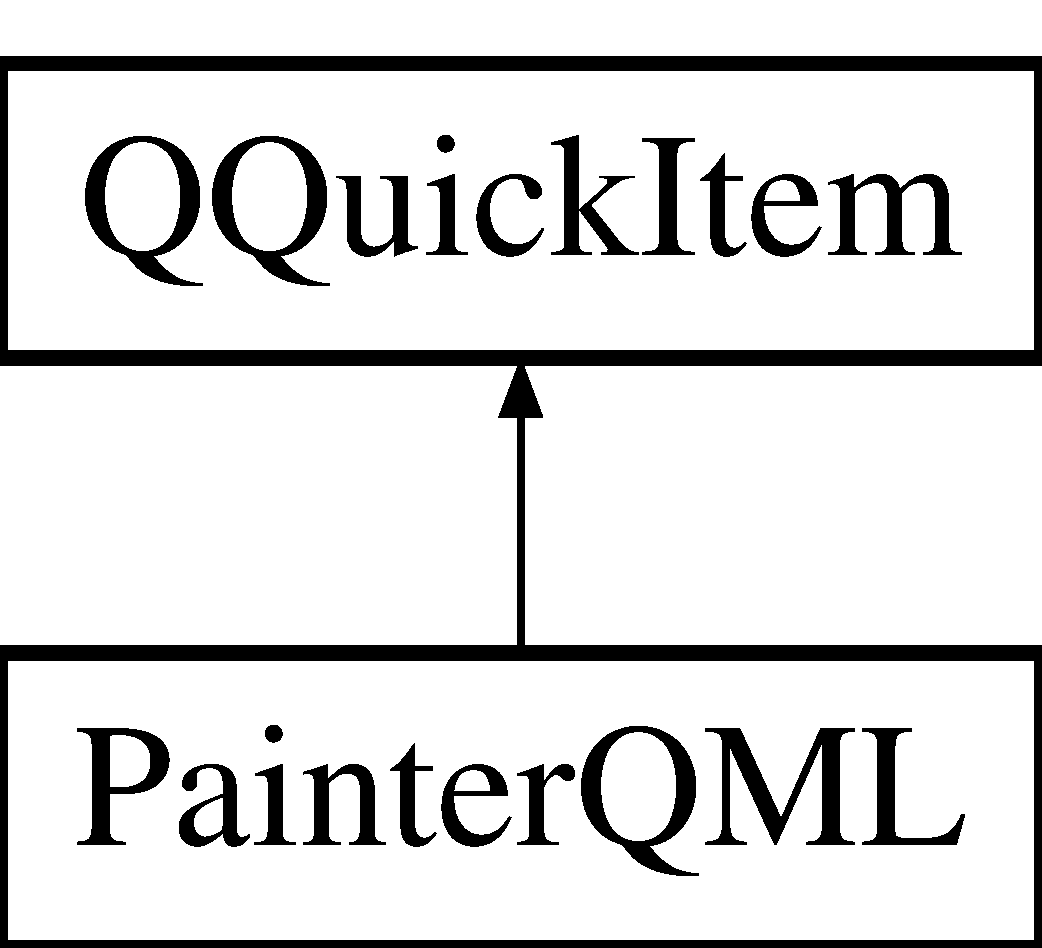
\includegraphics[height=2.000000cm]{class_painter_q_m_l}
\end{center}
\end{figure}
\subsection*{Signals}
\begin{DoxyCompactItemize}
\item 
void \hyperlink{class_painter_q_m_l_a9143d84bcf1b2c150c28983459916a70}{is\+Active\+Changed} ()
\item 
void \hyperlink{class_painter_q_m_l_a4f2212d4a85e7844c2c7c02ebc5bcf49}{is\+App\+Active\+Changed} ()
\item 
void \hyperlink{class_painter_q_m_l_a46f7374519937259609441c88a3b8b9f}{is\+Game\+Active\+Changed} ()
\item 
void \hyperlink{class_painter_q_m_l_a5fce3441beea885f9ba2a70b2f21f0ae}{scene\+Changed} ()
\end{DoxyCompactItemize}
\subsection*{Public Member Functions}
\begin{DoxyCompactItemize}
\item 
\hyperlink{class_painter_q_m_l_a6ce68afc41c75b1fc74da16890d9f797}{Painter\+Q\+M\+L} (Q\+Quick\+Item $\ast$parent=0)
\item 
virtual \hyperlink{class_painter_q_m_l_a2d0bd68f4b501927f65ec5ff2a06da64}{$\sim$\+Painter\+Q\+M\+L} ()
\item 
bool \hyperlink{class_painter_q_m_l_a69fecccc6056c3ee957219ffd63c193c}{event} (Q\+Event $\ast$ev) override
\begin{DoxyCompactList}\small\item\em Process incomming qt events. \end{DoxyCompactList}\item 
bool \hyperlink{class_painter_q_m_l_aad209e5ccfa2a6aa2a5dcd6148befb5b}{is\+Game\+Active} () const 
\begin{DoxyCompactList}\small\item\em Checks if our painter and therfor aour game is active.  Active means, that the game should be updated and rendered. But updates and rendering will be done only if there are no reasons against (e.\+g. The app is not active) \end{DoxyCompactList}\item 
void \hyperlink{class_painter_q_m_l_a303f544708d2041bc25e75db52e89736}{set\+Is\+Game\+Active} (bool active)
\begin{DoxyCompactList}\small\item\em Sets active state of \hyperlink{class_painter_q_m_l}{Painter\+Q\+M\+L}. \end{DoxyCompactList}\item 
Q\+Event\+::\+Type \hyperlink{class_painter_q_m_l_a7715bb2f3d638ff3d5e6e602a427b413}{painting\+Done\+Event\+Type} ()
\begin{DoxyCompactList}\small\item\em Queries registered event type, that should be send after rendering of current frame is done. \end{DoxyCompactList}\item 
Q\+\_\+\+I\+N\+V\+O\+K\+A\+B\+L\+E void \hyperlink{class_painter_q_m_l_a3dede2a01c6e90c51c9bfe69ac0d83bd}{reload\+Env\+Map} ()
\begin{DoxyCompactList}\small\item\em Reloads enviroment map of game using \hyperlink{class_config}{Config}. \end{DoxyCompactList}\item 
Q\+\_\+\+I\+N\+V\+O\+K\+A\+B\+L\+E void \hyperlink{class_painter_q_m_l_a401a8a8b2406679b61fe326a37e97b6a}{reset\+Timer} ()
\begin{DoxyCompactList}\small\item\em Resets update timer. This method is provided to allow manual resetting update time. \end{DoxyCompactList}\item 
\hyperlink{class_scene}{Scene} $\ast$ \hyperlink{class_painter_q_m_l_a6694ad2cfda4aefaffc0a3151a2b09dd}{scene} () const 
\begin{DoxyCompactList}\small\item\em The scene, that is painted by \hyperlink{class_painter_q_m_l}{Painter\+Q\+M\+L}. \end{DoxyCompactList}\item 
void \hyperlink{class_painter_q_m_l_a81288bcb25e5b985eea33b26ede7931a}{set\+Scene} (\hyperlink{class_scene}{Scene} $\ast$\hyperlink{class_painter_q_m_l_a59b4d398bc7880e59bc8296c2669aaab}{scene})
\begin{DoxyCompactList}\small\item\em Set the scene, which should be drawn by \hyperlink{class_painter_q_m_l}{Painter\+Q\+M\+L}. \end{DoxyCompactList}\item 
bool \hyperlink{class_painter_q_m_l_aea7b18053c645bf7c1eda6dd00715888}{is\+App\+Active} () const 
\begin{DoxyCompactList}\small\item\em Check if the \hyperlink{class_painter_q_m_l}{Painter\+Q\+M\+L} assumes the app is active or not. \end{DoxyCompactList}\item 
void \hyperlink{class_painter_q_m_l_a71be24e10048b456a566d2a3c9a8992b}{set\+Is\+App\+Active} (bool active)
\begin{DoxyCompactList}\small\item\em Inform the painter if app is active or not. Setting this attribute to false leads to pause of game (stop updating and rendering). \end{DoxyCompactList}\item 
bool \hyperlink{class_painter_q_m_l_a391bd3c26f57dfcb3177318595c89353}{is\+Active} () const 
\begin{DoxyCompactList}\small\item\em Checks if the our game will be updated. This means there is no reason, that our game is not updated. \end{DoxyCompactList}\end{DoxyCompactItemize}
\subsection*{Protected Slots}
\begin{DoxyCompactItemize}
\item 
void \hyperlink{class_painter_q_m_l_a4cfd22a52fc9e29d304c0ff7cea86744}{synchronize} ()
\begin{DoxyCompactList}\small\item\em Synchronize game logic and rendering.  Because Q\+M\+L uses different threads for ui and rendering, synchronization between these threads has to be done. This slot is connected by \hyperlink{class_painter_q_m_l}{Painter\+Q\+M\+L} to corresponding signals of Q\+Quick\+Item. \end{DoxyCompactList}\item 
void \hyperlink{class_painter_q_m_l_ab07e4719d2b05bbbfa48980b4854d190}{cleanup} ()
\begin{DoxyCompactList}\small\item\em Clean up the rendering thread ressources.  This slot is also connected by \hyperlink{class_painter_q_m_l}{Painter\+Q\+M\+L} to corresponding signal of Q\+Quick\+Item. \end{DoxyCompactList}\end{DoxyCompactItemize}
\subsection*{Protected Attributes}
\begin{DoxyCompactItemize}
\item 
bool \hyperlink{class_painter_q_m_l_a9acde8bb9dae70089141153efe168690}{m\+\_\+is\+App\+Active}
\item 
bool \hyperlink{class_painter_q_m_l_ab6aae1f8b8723eb4ebe7677ddc18ee11}{m\+\_\+is\+Game\+Active}
\item 
bool \hyperlink{class_painter_q_m_l_ae2e60015d5cc12a5fb5b5d0402189532}{m\+\_\+is\+Scene\+Deletion\+Required}
\item 
bool \hyperlink{class_painter_q_m_l_a3b291f7043ad8437baadf6d7be1c174d}{m\+\_\+is\+Update\+Pending}
\item 
\hyperlink{class_painter}{Painter} $\ast$ \hyperlink{class_painter_q_m_l_a6b21bae1a75260e121bc56cda38729c8}{m\+\_\+painter}
\item 
int \hyperlink{class_painter_q_m_l_a7a6641710573e4fa47dfdae13e87d58e}{m\+\_\+painting\+Done\+Event\+Type}
\item 
\hyperlink{class_scene}{Scene} $\ast$ \hyperlink{class_painter_q_m_l_a5eccac2ab6d9974a9ae94573ac7b19d6}{m\+\_\+scene}
\item 
Q\+Time $\ast$ \hyperlink{class_painter_q_m_l_ad4ced718f47b69f2344a5311ec87a156}{m\+\_\+time}
\end{DoxyCompactItemize}
\subsection*{Properties}
\begin{DoxyCompactItemize}
\item 
bool \hyperlink{class_painter_q_m_l_aab9bd8451a3cbfe6e8189994fd3dc329}{is\+Active}
\item 
bool \hyperlink{class_painter_q_m_l_a70ad19e1bbe24b9915c5f23366549a15}{is\+App\+Active}
\item 
bool \hyperlink{class_painter_q_m_l_ae878004adcc5589b4ffc81870a700f82}{is\+Game\+Active}
\item 
\hyperlink{class_scene}{Scene} \hyperlink{class_painter_q_m_l_a59b4d398bc7880e59bc8296c2669aaab}{scene}
\end{DoxyCompactItemize}


\subsection{Detailed Description}
The \hyperlink{class_painter_q_m_l}{Painter\+Q\+M\+L} class is responsible to make our game visible within Q\+M\+L using \hyperlink{class_painter}{Painter}.  This class is intended to be added and created within Q\+M\+L. As the element showing our game it recognizes(?) resize events and update events needed by our application. Also it keeps our rendering alive. Furthermore it is the interface between game logic and rendering. 

\subsection{Constructor \& Destructor Documentation}
\hypertarget{class_painter_q_m_l_a6ce68afc41c75b1fc74da16890d9f797}{}\index{Painter\+Q\+M\+L@{Painter\+Q\+M\+L}!Painter\+Q\+M\+L@{Painter\+Q\+M\+L}}
\index{Painter\+Q\+M\+L@{Painter\+Q\+M\+L}!Painter\+Q\+M\+L@{Painter\+Q\+M\+L}}
\subsubsection[{Painter\+Q\+M\+L}]{\setlength{\rightskip}{0pt plus 5cm}Painter\+Q\+M\+L\+::\+Painter\+Q\+M\+L (
\begin{DoxyParamCaption}
\item[{Q\+Quick\+Item $\ast$}]{parent = {\ttfamily 0}}
\end{DoxyParamCaption}
)\hspace{0.3cm}{\ttfamily [explicit]}}\label{class_painter_q_m_l_a6ce68afc41c75b1fc74da16890d9f797}
\hypertarget{class_painter_q_m_l_a2d0bd68f4b501927f65ec5ff2a06da64}{}\index{Painter\+Q\+M\+L@{Painter\+Q\+M\+L}!````~Painter\+Q\+M\+L@{$\sim$\+Painter\+Q\+M\+L}}
\index{````~Painter\+Q\+M\+L@{$\sim$\+Painter\+Q\+M\+L}!Painter\+Q\+M\+L@{Painter\+Q\+M\+L}}
\subsubsection[{$\sim$\+Painter\+Q\+M\+L}]{\setlength{\rightskip}{0pt plus 5cm}Painter\+Q\+M\+L\+::$\sim$\+Painter\+Q\+M\+L (
\begin{DoxyParamCaption}
{}
\end{DoxyParamCaption}
)\hspace{0.3cm}{\ttfamily [virtual]}}\label{class_painter_q_m_l_a2d0bd68f4b501927f65ec5ff2a06da64}


\subsection{Member Function Documentation}
\hypertarget{class_painter_q_m_l_ab07e4719d2b05bbbfa48980b4854d190}{}\index{Painter\+Q\+M\+L@{Painter\+Q\+M\+L}!cleanup@{cleanup}}
\index{cleanup@{cleanup}!Painter\+Q\+M\+L@{Painter\+Q\+M\+L}}
\subsubsection[{cleanup}]{\setlength{\rightskip}{0pt plus 5cm}void Painter\+Q\+M\+L\+::cleanup (
\begin{DoxyParamCaption}
{}
\end{DoxyParamCaption}
)\hspace{0.3cm}{\ttfamily [protected]}, {\ttfamily [slot]}}\label{class_painter_q_m_l_ab07e4719d2b05bbbfa48980b4854d190}


Clean up the rendering thread ressources.  This slot is also connected by \hyperlink{class_painter_q_m_l}{Painter\+Q\+M\+L} to corresponding signal of Q\+Quick\+Item. 

\hypertarget{class_painter_q_m_l_a69fecccc6056c3ee957219ffd63c193c}{}\index{Painter\+Q\+M\+L@{Painter\+Q\+M\+L}!event@{event}}
\index{event@{event}!Painter\+Q\+M\+L@{Painter\+Q\+M\+L}}
\subsubsection[{event}]{\setlength{\rightskip}{0pt plus 5cm}bool Painter\+Q\+M\+L\+::event (
\begin{DoxyParamCaption}
\item[{Q\+Event $\ast$}]{ev}
\end{DoxyParamCaption}
)\hspace{0.3cm}{\ttfamily [override]}}\label{class_painter_q_m_l_a69fecccc6056c3ee957219ffd63c193c}


Process incomming qt events. 


\begin{DoxyParams}{Parameters}
{\em ev} & Event that should be handled. \\
\hline
\end{DoxyParams}
\begin{DoxyReturn}{Returns}
Returns true if the event was handled by Q\+Object. 
\end{DoxyReturn}
\hypertarget{class_painter_q_m_l_a391bd3c26f57dfcb3177318595c89353}{}\index{Painter\+Q\+M\+L@{Painter\+Q\+M\+L}!is\+Active@{is\+Active}}
\index{is\+Active@{is\+Active}!Painter\+Q\+M\+L@{Painter\+Q\+M\+L}}
\subsubsection[{is\+Active}]{\setlength{\rightskip}{0pt plus 5cm}bool Painter\+Q\+M\+L\+::is\+Active (
\begin{DoxyParamCaption}
{}
\end{DoxyParamCaption}
) const}\label{class_painter_q_m_l_a391bd3c26f57dfcb3177318595c89353}


Checks if the our game will be updated. This means there is no reason, that our game is not updated. 

\begin{DoxyReturn}{Returns}

\end{DoxyReturn}
\hypertarget{class_painter_q_m_l_a9143d84bcf1b2c150c28983459916a70}{}\index{Painter\+Q\+M\+L@{Painter\+Q\+M\+L}!is\+Active\+Changed@{is\+Active\+Changed}}
\index{is\+Active\+Changed@{is\+Active\+Changed}!Painter\+Q\+M\+L@{Painter\+Q\+M\+L}}
\subsubsection[{is\+Active\+Changed}]{\setlength{\rightskip}{0pt plus 5cm}void Painter\+Q\+M\+L\+::is\+Active\+Changed (
\begin{DoxyParamCaption}
{}
\end{DoxyParamCaption}
)\hspace{0.3cm}{\ttfamily [signal]}}\label{class_painter_q_m_l_a9143d84bcf1b2c150c28983459916a70}
\hypertarget{class_painter_q_m_l_aea7b18053c645bf7c1eda6dd00715888}{}\index{Painter\+Q\+M\+L@{Painter\+Q\+M\+L}!is\+App\+Active@{is\+App\+Active}}
\index{is\+App\+Active@{is\+App\+Active}!Painter\+Q\+M\+L@{Painter\+Q\+M\+L}}
\subsubsection[{is\+App\+Active}]{\setlength{\rightskip}{0pt plus 5cm}bool Painter\+Q\+M\+L\+::is\+App\+Active (
\begin{DoxyParamCaption}
{}
\end{DoxyParamCaption}
) const}\label{class_painter_q_m_l_aea7b18053c645bf7c1eda6dd00715888}


Check if the \hyperlink{class_painter_q_m_l}{Painter\+Q\+M\+L} assumes the app is active or not. 

\begin{DoxyReturn}{Returns}

\end{DoxyReturn}
\hypertarget{class_painter_q_m_l_a4f2212d4a85e7844c2c7c02ebc5bcf49}{}\index{Painter\+Q\+M\+L@{Painter\+Q\+M\+L}!is\+App\+Active\+Changed@{is\+App\+Active\+Changed}}
\index{is\+App\+Active\+Changed@{is\+App\+Active\+Changed}!Painter\+Q\+M\+L@{Painter\+Q\+M\+L}}
\subsubsection[{is\+App\+Active\+Changed}]{\setlength{\rightskip}{0pt plus 5cm}void Painter\+Q\+M\+L\+::is\+App\+Active\+Changed (
\begin{DoxyParamCaption}
{}
\end{DoxyParamCaption}
)\hspace{0.3cm}{\ttfamily [signal]}}\label{class_painter_q_m_l_a4f2212d4a85e7844c2c7c02ebc5bcf49}
\hypertarget{class_painter_q_m_l_aad209e5ccfa2a6aa2a5dcd6148befb5b}{}\index{Painter\+Q\+M\+L@{Painter\+Q\+M\+L}!is\+Game\+Active@{is\+Game\+Active}}
\index{is\+Game\+Active@{is\+Game\+Active}!Painter\+Q\+M\+L@{Painter\+Q\+M\+L}}
\subsubsection[{is\+Game\+Active}]{\setlength{\rightskip}{0pt plus 5cm}bool Painter\+Q\+M\+L\+::is\+Game\+Active (
\begin{DoxyParamCaption}
{}
\end{DoxyParamCaption}
) const}\label{class_painter_q_m_l_aad209e5ccfa2a6aa2a5dcd6148befb5b}


Checks if our painter and therfor aour game is active.  Active means, that the game should be updated and rendered. But updates and rendering will be done only if there are no reasons against (e.\+g. The app is not active) 

\begin{DoxyReturn}{Returns}
Returns true if \hyperlink{class_painter_q_m_l}{Painter\+Q\+M\+L} is active. 
\end{DoxyReturn}
\begin{DoxySeeAlso}{See also}
\hyperlink{class_painter_q_m_l_a70ad19e1bbe24b9915c5f23366549a15}{is\+App\+Active()}, \hyperlink{class_painter_q_m_l_aab9bd8451a3cbfe6e8189994fd3dc329}{is\+Active()} 
\end{DoxySeeAlso}
\hypertarget{class_painter_q_m_l_a46f7374519937259609441c88a3b8b9f}{}\index{Painter\+Q\+M\+L@{Painter\+Q\+M\+L}!is\+Game\+Active\+Changed@{is\+Game\+Active\+Changed}}
\index{is\+Game\+Active\+Changed@{is\+Game\+Active\+Changed}!Painter\+Q\+M\+L@{Painter\+Q\+M\+L}}
\subsubsection[{is\+Game\+Active\+Changed}]{\setlength{\rightskip}{0pt plus 5cm}void Painter\+Q\+M\+L\+::is\+Game\+Active\+Changed (
\begin{DoxyParamCaption}
{}
\end{DoxyParamCaption}
)\hspace{0.3cm}{\ttfamily [signal]}}\label{class_painter_q_m_l_a46f7374519937259609441c88a3b8b9f}
\hypertarget{class_painter_q_m_l_a7715bb2f3d638ff3d5e6e602a427b413}{}\index{Painter\+Q\+M\+L@{Painter\+Q\+M\+L}!painting\+Done\+Event\+Type@{painting\+Done\+Event\+Type}}
\index{painting\+Done\+Event\+Type@{painting\+Done\+Event\+Type}!Painter\+Q\+M\+L@{Painter\+Q\+M\+L}}
\subsubsection[{painting\+Done\+Event\+Type}]{\setlength{\rightskip}{0pt plus 5cm}Q\+Event\+::\+Type Painter\+Q\+M\+L\+::painting\+Done\+Event\+Type (
\begin{DoxyParamCaption}
{}
\end{DoxyParamCaption}
)}\label{class_painter_q_m_l_a7715bb2f3d638ff3d5e6e602a427b413}


Queries registered event type, that should be send after rendering of current frame is done. 

\begin{DoxyReturn}{Returns}
Returns registered event type 
\end{DoxyReturn}
\hypertarget{class_painter_q_m_l_a3dede2a01c6e90c51c9bfe69ac0d83bd}{}\index{Painter\+Q\+M\+L@{Painter\+Q\+M\+L}!reload\+Env\+Map@{reload\+Env\+Map}}
\index{reload\+Env\+Map@{reload\+Env\+Map}!Painter\+Q\+M\+L@{Painter\+Q\+M\+L}}
\subsubsection[{reload\+Env\+Map}]{\setlength{\rightskip}{0pt plus 5cm}void Painter\+Q\+M\+L\+::reload\+Env\+Map (
\begin{DoxyParamCaption}
{}
\end{DoxyParamCaption}
)}\label{class_painter_q_m_l_a3dede2a01c6e90c51c9bfe69ac0d83bd}


Reloads enviroment map of game using \hyperlink{class_config}{Config}. 

\hypertarget{class_painter_q_m_l_a401a8a8b2406679b61fe326a37e97b6a}{}\index{Painter\+Q\+M\+L@{Painter\+Q\+M\+L}!reset\+Timer@{reset\+Timer}}
\index{reset\+Timer@{reset\+Timer}!Painter\+Q\+M\+L@{Painter\+Q\+M\+L}}
\subsubsection[{reset\+Timer}]{\setlength{\rightskip}{0pt plus 5cm}void Painter\+Q\+M\+L\+::reset\+Timer (
\begin{DoxyParamCaption}
{}
\end{DoxyParamCaption}
)}\label{class_painter_q_m_l_a401a8a8b2406679b61fe326a37e97b6a}


Resets update timer. This method is provided to allow manual resetting update time. 

\hypertarget{class_painter_q_m_l_a6694ad2cfda4aefaffc0a3151a2b09dd}{}\index{Painter\+Q\+M\+L@{Painter\+Q\+M\+L}!scene@{scene}}
\index{scene@{scene}!Painter\+Q\+M\+L@{Painter\+Q\+M\+L}}
\subsubsection[{scene}]{\setlength{\rightskip}{0pt plus 5cm}{\bf Scene}$\ast$ Painter\+Q\+M\+L\+::scene (
\begin{DoxyParamCaption}
{}
\end{DoxyParamCaption}
) const}\label{class_painter_q_m_l_a6694ad2cfda4aefaffc0a3151a2b09dd}


The scene, that is painted by \hyperlink{class_painter_q_m_l}{Painter\+Q\+M\+L}. 

\begin{DoxyReturn}{Returns}

\end{DoxyReturn}
\hypertarget{class_painter_q_m_l_a5fce3441beea885f9ba2a70b2f21f0ae}{}\index{Painter\+Q\+M\+L@{Painter\+Q\+M\+L}!scene\+Changed@{scene\+Changed}}
\index{scene\+Changed@{scene\+Changed}!Painter\+Q\+M\+L@{Painter\+Q\+M\+L}}
\subsubsection[{scene\+Changed}]{\setlength{\rightskip}{0pt plus 5cm}void Painter\+Q\+M\+L\+::scene\+Changed (
\begin{DoxyParamCaption}
{}
\end{DoxyParamCaption}
)\hspace{0.3cm}{\ttfamily [signal]}}\label{class_painter_q_m_l_a5fce3441beea885f9ba2a70b2f21f0ae}
\hypertarget{class_painter_q_m_l_a71be24e10048b456a566d2a3c9a8992b}{}\index{Painter\+Q\+M\+L@{Painter\+Q\+M\+L}!set\+Is\+App\+Active@{set\+Is\+App\+Active}}
\index{set\+Is\+App\+Active@{set\+Is\+App\+Active}!Painter\+Q\+M\+L@{Painter\+Q\+M\+L}}
\subsubsection[{set\+Is\+App\+Active}]{\setlength{\rightskip}{0pt plus 5cm}void Painter\+Q\+M\+L\+::set\+Is\+App\+Active (
\begin{DoxyParamCaption}
\item[{bool}]{active}
\end{DoxyParamCaption}
)}\label{class_painter_q_m_l_a71be24e10048b456a566d2a3c9a8992b}


Inform the painter if app is active or not. Setting this attribute to false leads to pause of game (stop updating and rendering). 


\begin{DoxyParams}{Parameters}
{\em active} & \\
\hline
\end{DoxyParams}
\hypertarget{class_painter_q_m_l_a303f544708d2041bc25e75db52e89736}{}\index{Painter\+Q\+M\+L@{Painter\+Q\+M\+L}!set\+Is\+Game\+Active@{set\+Is\+Game\+Active}}
\index{set\+Is\+Game\+Active@{set\+Is\+Game\+Active}!Painter\+Q\+M\+L@{Painter\+Q\+M\+L}}
\subsubsection[{set\+Is\+Game\+Active}]{\setlength{\rightskip}{0pt plus 5cm}void Painter\+Q\+M\+L\+::set\+Is\+Game\+Active (
\begin{DoxyParamCaption}
\item[{bool}]{active}
\end{DoxyParamCaption}
)}\label{class_painter_q_m_l_a303f544708d2041bc25e75db52e89736}


Sets active state of \hyperlink{class_painter_q_m_l}{Painter\+Q\+M\+L}. 


\begin{DoxyParams}{Parameters}
{\em active} & \\
\hline
\end{DoxyParams}
\hypertarget{class_painter_q_m_l_a81288bcb25e5b985eea33b26ede7931a}{}\index{Painter\+Q\+M\+L@{Painter\+Q\+M\+L}!set\+Scene@{set\+Scene}}
\index{set\+Scene@{set\+Scene}!Painter\+Q\+M\+L@{Painter\+Q\+M\+L}}
\subsubsection[{set\+Scene}]{\setlength{\rightskip}{0pt plus 5cm}void Painter\+Q\+M\+L\+::set\+Scene (
\begin{DoxyParamCaption}
\item[{{\bf Scene} $\ast$}]{scene}
\end{DoxyParamCaption}
)}\label{class_painter_q_m_l_a81288bcb25e5b985eea33b26ede7931a}


Set the scene, which should be drawn by \hyperlink{class_painter_q_m_l}{Painter\+Q\+M\+L}. 


\begin{DoxyParams}{Parameters}
{\em scene} & \\
\hline
\end{DoxyParams}
\hypertarget{class_painter_q_m_l_a4cfd22a52fc9e29d304c0ff7cea86744}{}\index{Painter\+Q\+M\+L@{Painter\+Q\+M\+L}!synchronize@{synchronize}}
\index{synchronize@{synchronize}!Painter\+Q\+M\+L@{Painter\+Q\+M\+L}}
\subsubsection[{synchronize}]{\setlength{\rightskip}{0pt plus 5cm}void Painter\+Q\+M\+L\+::synchronize (
\begin{DoxyParamCaption}
{}
\end{DoxyParamCaption}
)\hspace{0.3cm}{\ttfamily [protected]}, {\ttfamily [slot]}}\label{class_painter_q_m_l_a4cfd22a52fc9e29d304c0ff7cea86744}


Synchronize game logic and rendering.  Because Q\+M\+L uses different threads for ui and rendering, synchronization between these threads has to be done. This slot is connected by \hyperlink{class_painter_q_m_l}{Painter\+Q\+M\+L} to corresponding signals of Q\+Quick\+Item. 



\subsection{Member Data Documentation}
\hypertarget{class_painter_q_m_l_a9acde8bb9dae70089141153efe168690}{}\index{Painter\+Q\+M\+L@{Painter\+Q\+M\+L}!m\+\_\+is\+App\+Active@{m\+\_\+is\+App\+Active}}
\index{m\+\_\+is\+App\+Active@{m\+\_\+is\+App\+Active}!Painter\+Q\+M\+L@{Painter\+Q\+M\+L}}
\subsubsection[{m\+\_\+is\+App\+Active}]{\setlength{\rightskip}{0pt plus 5cm}bool Painter\+Q\+M\+L\+::m\+\_\+is\+App\+Active\hspace{0.3cm}{\ttfamily [protected]}}\label{class_painter_q_m_l_a9acde8bb9dae70089141153efe168690}
\hypertarget{class_painter_q_m_l_ab6aae1f8b8723eb4ebe7677ddc18ee11}{}\index{Painter\+Q\+M\+L@{Painter\+Q\+M\+L}!m\+\_\+is\+Game\+Active@{m\+\_\+is\+Game\+Active}}
\index{m\+\_\+is\+Game\+Active@{m\+\_\+is\+Game\+Active}!Painter\+Q\+M\+L@{Painter\+Q\+M\+L}}
\subsubsection[{m\+\_\+is\+Game\+Active}]{\setlength{\rightskip}{0pt plus 5cm}bool Painter\+Q\+M\+L\+::m\+\_\+is\+Game\+Active\hspace{0.3cm}{\ttfamily [protected]}}\label{class_painter_q_m_l_ab6aae1f8b8723eb4ebe7677ddc18ee11}
\hypertarget{class_painter_q_m_l_ae2e60015d5cc12a5fb5b5d0402189532}{}\index{Painter\+Q\+M\+L@{Painter\+Q\+M\+L}!m\+\_\+is\+Scene\+Deletion\+Required@{m\+\_\+is\+Scene\+Deletion\+Required}}
\index{m\+\_\+is\+Scene\+Deletion\+Required@{m\+\_\+is\+Scene\+Deletion\+Required}!Painter\+Q\+M\+L@{Painter\+Q\+M\+L}}
\subsubsection[{m\+\_\+is\+Scene\+Deletion\+Required}]{\setlength{\rightskip}{0pt plus 5cm}bool Painter\+Q\+M\+L\+::m\+\_\+is\+Scene\+Deletion\+Required\hspace{0.3cm}{\ttfamily [protected]}}\label{class_painter_q_m_l_ae2e60015d5cc12a5fb5b5d0402189532}
\hypertarget{class_painter_q_m_l_a3b291f7043ad8437baadf6d7be1c174d}{}\index{Painter\+Q\+M\+L@{Painter\+Q\+M\+L}!m\+\_\+is\+Update\+Pending@{m\+\_\+is\+Update\+Pending}}
\index{m\+\_\+is\+Update\+Pending@{m\+\_\+is\+Update\+Pending}!Painter\+Q\+M\+L@{Painter\+Q\+M\+L}}
\subsubsection[{m\+\_\+is\+Update\+Pending}]{\setlength{\rightskip}{0pt plus 5cm}bool Painter\+Q\+M\+L\+::m\+\_\+is\+Update\+Pending\hspace{0.3cm}{\ttfamily [protected]}}\label{class_painter_q_m_l_a3b291f7043ad8437baadf6d7be1c174d}
\hypertarget{class_painter_q_m_l_a6b21bae1a75260e121bc56cda38729c8}{}\index{Painter\+Q\+M\+L@{Painter\+Q\+M\+L}!m\+\_\+painter@{m\+\_\+painter}}
\index{m\+\_\+painter@{m\+\_\+painter}!Painter\+Q\+M\+L@{Painter\+Q\+M\+L}}
\subsubsection[{m\+\_\+painter}]{\setlength{\rightskip}{0pt plus 5cm}{\bf Painter}$\ast$ Painter\+Q\+M\+L\+::m\+\_\+painter\hspace{0.3cm}{\ttfamily [protected]}}\label{class_painter_q_m_l_a6b21bae1a75260e121bc56cda38729c8}
\hypertarget{class_painter_q_m_l_a7a6641710573e4fa47dfdae13e87d58e}{}\index{Painter\+Q\+M\+L@{Painter\+Q\+M\+L}!m\+\_\+painting\+Done\+Event\+Type@{m\+\_\+painting\+Done\+Event\+Type}}
\index{m\+\_\+painting\+Done\+Event\+Type@{m\+\_\+painting\+Done\+Event\+Type}!Painter\+Q\+M\+L@{Painter\+Q\+M\+L}}
\subsubsection[{m\+\_\+painting\+Done\+Event\+Type}]{\setlength{\rightskip}{0pt plus 5cm}int Painter\+Q\+M\+L\+::m\+\_\+painting\+Done\+Event\+Type\hspace{0.3cm}{\ttfamily [protected]}}\label{class_painter_q_m_l_a7a6641710573e4fa47dfdae13e87d58e}
\hypertarget{class_painter_q_m_l_a5eccac2ab6d9974a9ae94573ac7b19d6}{}\index{Painter\+Q\+M\+L@{Painter\+Q\+M\+L}!m\+\_\+scene@{m\+\_\+scene}}
\index{m\+\_\+scene@{m\+\_\+scene}!Painter\+Q\+M\+L@{Painter\+Q\+M\+L}}
\subsubsection[{m\+\_\+scene}]{\setlength{\rightskip}{0pt plus 5cm}{\bf Scene}$\ast$ Painter\+Q\+M\+L\+::m\+\_\+scene\hspace{0.3cm}{\ttfamily [protected]}}\label{class_painter_q_m_l_a5eccac2ab6d9974a9ae94573ac7b19d6}
\hypertarget{class_painter_q_m_l_ad4ced718f47b69f2344a5311ec87a156}{}\index{Painter\+Q\+M\+L@{Painter\+Q\+M\+L}!m\+\_\+time@{m\+\_\+time}}
\index{m\+\_\+time@{m\+\_\+time}!Painter\+Q\+M\+L@{Painter\+Q\+M\+L}}
\subsubsection[{m\+\_\+time}]{\setlength{\rightskip}{0pt plus 5cm}Q\+Time$\ast$ Painter\+Q\+M\+L\+::m\+\_\+time\hspace{0.3cm}{\ttfamily [protected]}}\label{class_painter_q_m_l_ad4ced718f47b69f2344a5311ec87a156}


\subsection{Property Documentation}
\hypertarget{class_painter_q_m_l_aab9bd8451a3cbfe6e8189994fd3dc329}{}\index{Painter\+Q\+M\+L@{Painter\+Q\+M\+L}!is\+Active@{is\+Active}}
\index{is\+Active@{is\+Active}!Painter\+Q\+M\+L@{Painter\+Q\+M\+L}}
\subsubsection[{is\+Active}]{\setlength{\rightskip}{0pt plus 5cm}bool Painter\+Q\+M\+L\+::is\+Active\hspace{0.3cm}{\ttfamily [read]}}\label{class_painter_q_m_l_aab9bd8451a3cbfe6e8189994fd3dc329}
\hypertarget{class_painter_q_m_l_a70ad19e1bbe24b9915c5f23366549a15}{}\index{Painter\+Q\+M\+L@{Painter\+Q\+M\+L}!is\+App\+Active@{is\+App\+Active}}
\index{is\+App\+Active@{is\+App\+Active}!Painter\+Q\+M\+L@{Painter\+Q\+M\+L}}
\subsubsection[{is\+App\+Active}]{\setlength{\rightskip}{0pt plus 5cm}bool Painter\+Q\+M\+L\+::is\+App\+Active\hspace{0.3cm}{\ttfamily [read]}, {\ttfamily [write]}}\label{class_painter_q_m_l_a70ad19e1bbe24b9915c5f23366549a15}
\hypertarget{class_painter_q_m_l_ae878004adcc5589b4ffc81870a700f82}{}\index{Painter\+Q\+M\+L@{Painter\+Q\+M\+L}!is\+Game\+Active@{is\+Game\+Active}}
\index{is\+Game\+Active@{is\+Game\+Active}!Painter\+Q\+M\+L@{Painter\+Q\+M\+L}}
\subsubsection[{is\+Game\+Active}]{\setlength{\rightskip}{0pt plus 5cm}bool Painter\+Q\+M\+L\+::is\+Game\+Active\hspace{0.3cm}{\ttfamily [read]}, {\ttfamily [write]}}\label{class_painter_q_m_l_ae878004adcc5589b4ffc81870a700f82}
\hypertarget{class_painter_q_m_l_a59b4d398bc7880e59bc8296c2669aaab}{}\index{Painter\+Q\+M\+L@{Painter\+Q\+M\+L}!scene@{scene}}
\index{scene@{scene}!Painter\+Q\+M\+L@{Painter\+Q\+M\+L}}
\subsubsection[{scene}]{\setlength{\rightskip}{0pt plus 5cm}{\bf Scene} $\ast$ Painter\+Q\+M\+L\+::scene\hspace{0.3cm}{\ttfamily [read]}, {\ttfamily [write]}}\label{class_painter_q_m_l_a59b4d398bc7880e59bc8296c2669aaab}


The documentation for this class was generated from the following files\+:\begin{DoxyCompactItemize}
\item 
Game-\/\+Programming-\/\+W\+S2014/gem\+Illuminator/\hyperlink{painterqml_8h}{painterqml.\+h}\item 
Game-\/\+Programming-\/\+W\+S2014/gem\+Illuminator/\hyperlink{painterqml_8cpp}{painterqml.\+cpp}\end{DoxyCompactItemize}

\hypertarget{class_player}{\section{Player Class Reference}
\label{class_player}\index{Player@{Player}}
}


The \hyperlink{class_player}{Player} class' only responsibilities are riding on lightrays and updating the camera.  




{\ttfamily \#include $<$player.\+h$>$}

Inheritance diagram for Player\+:\begin{figure}[H]
\begin{center}
\leavevmode
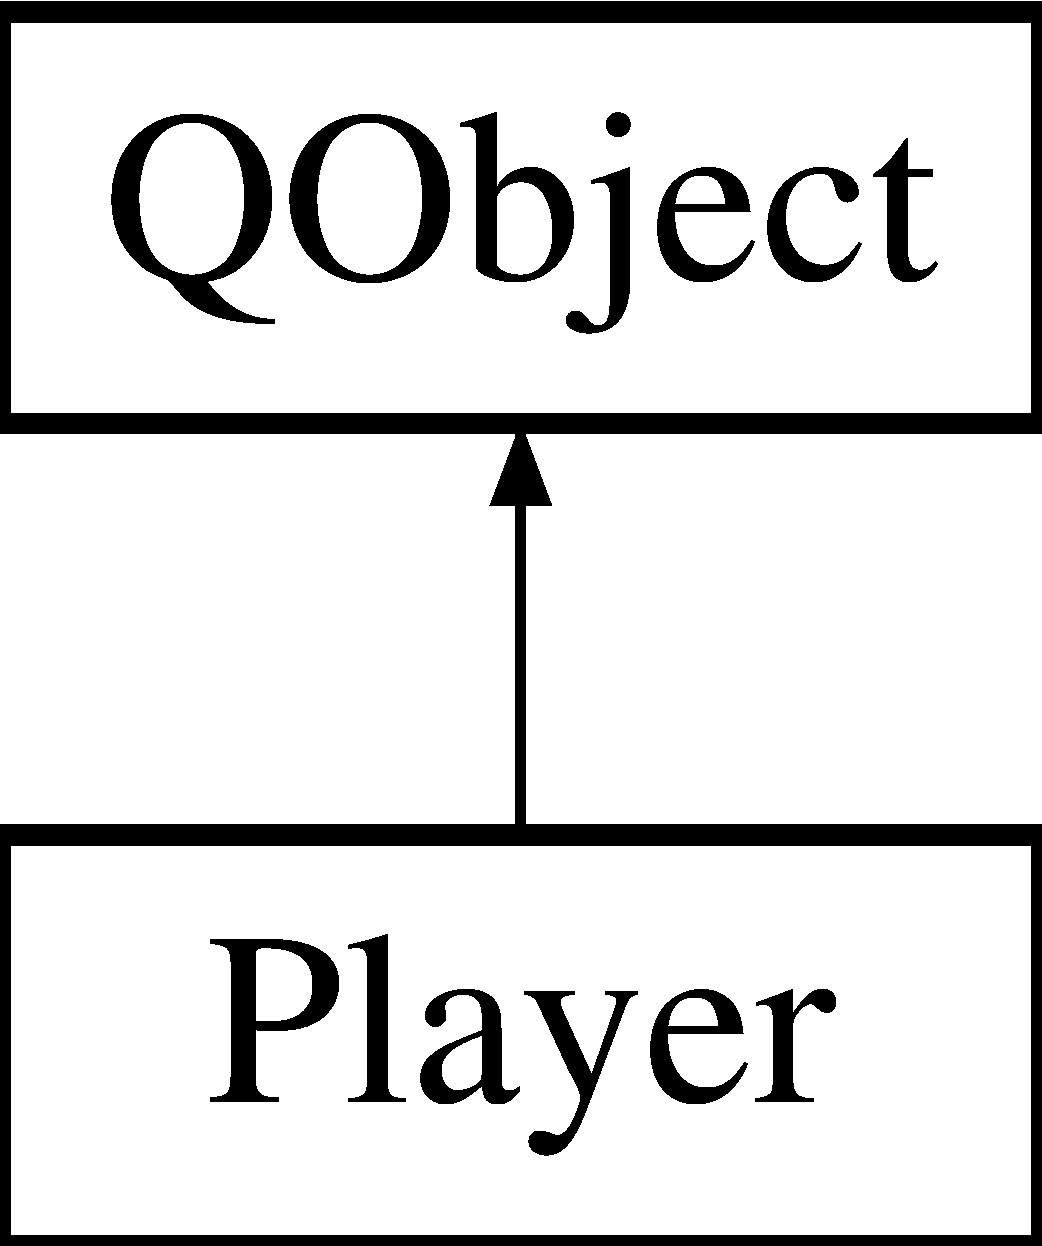
\includegraphics[height=2.000000cm]{class_player}
\end{center}
\end{figure}
\subsection*{Public Slots}
\begin{DoxyCompactItemize}
\item 
\hyperlink{class_camera}{Camera} $\ast$ \hyperlink{class_player_a10605ebcab0fac1b542d1bd8f3d23acd}{camera} () const 
\begin{DoxyCompactList}\small\item\em The camera which is updated by player. \end{DoxyCompactList}\item 
void \hyperlink{class_player_af5e57b3a9719cd999aff21d59355be52}{set\+Camera} (\hyperlink{class_camera}{Camera} $\ast$camera)
\begin{DoxyCompactList}\small\item\em Sets the camera, that should be updated by player. The player does not take ownership of camera. \end{DoxyCompactList}\item 
qreal \hyperlink{class_player_a836e1afdde2c379b964bcf5d3811f0da}{velocity} () const 
\begin{DoxyCompactList}\small\item\em The velocity of player. \end{DoxyCompactList}\item 
void \hyperlink{class_player_ae2d5423c7bf6c6c924a451dc1cdab6aa}{set\+Velocity} (qreal velocity)
\begin{DoxyCompactList}\small\item\em Sets velocity of player. \end{DoxyCompactList}\end{DoxyCompactItemize}
\subsection*{Signals}
\begin{DoxyCompactItemize}
\item 
void \hyperlink{class_player_aef620bc75871b32311560a7b2a31c144}{camera\+Changed} ()
\item 
void \hyperlink{class_player_a22ae3d9604e92fa12cfad39fe40e8651}{velocity\+Changed} ()
\end{DoxyCompactItemize}
\subsection*{Public Member Functions}
\begin{DoxyCompactItemize}
\item 
\hyperlink{class_player_a5c2a46dbacbc28b7cfbe352b6c0db644}{Player} (Q\+Object $\ast$parent=0)
\item 
virtual \hyperlink{class_player_a749d2c00e1fe0f5c2746f7505a58c062}{$\sim$\+Player} ()
\item 
void \hyperlink{class_player_a6dcd0b9f4d678260314878ab20ce6e09}{move\+On\+Ray} (const \hyperlink{class_light_ray}{Light\+Ray} \&ray, int time\+Difference\+In\+Milliseconds)
\begin{DoxyCompactList}\small\item\em Moves the player along a ray. \end{DoxyCompactList}\item 
void \hyperlink{class_player_a38269e0706f91b71c6e8f8373c397969}{move\+To\+Start\+Point\+On\+Ray} (const \hyperlink{class_light_ray}{Light\+Ray} \&ray)
\begin{DoxyCompactList}\small\item\em Sest the player to ray.\+start\+Position() and updates the camera accordingly. \end{DoxyCompactList}\item 
void \hyperlink{class_player_a0a4ebefb0f7593d79573ddcfe68e8e2f}{move\+To\+End\+Point\+On\+Ray} (const \hyperlink{class_light_ray}{Light\+Ray} \&ray)
\begin{DoxyCompactList}\small\item\em Sets the player to ray.\+end\+Position() and updates the camera accordingly. \end{DoxyCompactList}\item 
const Q\+Vector3\+D \& \hyperlink{class_player_a0c307c67d3c6d64ee9c5b724c1e2b095}{position} () const 
\begin{DoxyCompactList}\small\item\em The position of player in world coordinates. \end{DoxyCompactList}\item 
void \hyperlink{class_player_a0cb33ddb87038b4e2af648e1b884d79f}{set\+Position} (const Q\+Vector3\+D \&\hyperlink{class_player_a0c307c67d3c6d64ee9c5b724c1e2b095}{position})
\item 
void \hyperlink{class_player_ae51ad40372e26d33351c02d77a1aba63}{set\+View\+Direction} (const Q\+Vector3\+D \&view\+Direction)
\begin{DoxyCompactList}\small\item\em Set view direction to provided value. For now this value should be the same like the direction of followed lightray. \end{DoxyCompactList}\end{DoxyCompactItemize}
\subsection*{Protected Member Functions}
\begin{DoxyCompactItemize}
\item 
void \hyperlink{class_player_a557b70acbd3cb1f71218390f7e90105c}{update\+Camera\+For\+Point\+On\+Ray} (const Q\+Vector3\+D \&point, const \hyperlink{class_light_ray}{Light\+Ray} \&ray)
\begin{DoxyCompactList}\small\item\em Updates the camera position for given point on ray. \end{DoxyCompactList}\end{DoxyCompactItemize}
\subsection*{Protected Attributes}
\begin{DoxyCompactItemize}
\item 
qreal \hyperlink{class_player_a962e97e5fd3fe1c2db4e7e2066dbe61c}{m\+\_\+velocity}
\item 
Q\+Vector3\+D $\ast$ \hyperlink{class_player_a9dc251e6a6d9a7f49c3f2ad5b64a7780}{m\+\_\+position}
\item 
\hyperlink{class_camera}{Camera} $\ast$ \hyperlink{class_player_a7721626a1c43592bfcb0c81a836f7aad}{m\+\_\+camera}
\end{DoxyCompactItemize}


\subsection{Detailed Description}
The \hyperlink{class_player}{Player} class' only responsibilities are riding on lightrays and updating the camera. 

\subsection{Constructor \& Destructor Documentation}
\hypertarget{class_player_a5c2a46dbacbc28b7cfbe352b6c0db644}{\index{Player@{Player}!Player@{Player}}
\index{Player@{Player}!Player@{Player}}
\subsubsection[{Player}]{\setlength{\rightskip}{0pt plus 5cm}Player\+::\+Player (
\begin{DoxyParamCaption}
\item[{Q\+Object $\ast$}]{parent = {\ttfamily 0}}
\end{DoxyParamCaption}
)\hspace{0.3cm}{\ttfamily [explicit]}}}\label{class_player_a5c2a46dbacbc28b7cfbe352b6c0db644}
\hypertarget{class_player_a749d2c00e1fe0f5c2746f7505a58c062}{\index{Player@{Player}!````~Player@{$\sim$\+Player}}
\index{````~Player@{$\sim$\+Player}!Player@{Player}}
\subsubsection[{$\sim$\+Player}]{\setlength{\rightskip}{0pt plus 5cm}Player\+::$\sim$\+Player (
\begin{DoxyParamCaption}
{}
\end{DoxyParamCaption}
)\hspace{0.3cm}{\ttfamily [virtual]}}}\label{class_player_a749d2c00e1fe0f5c2746f7505a58c062}


\subsection{Member Function Documentation}
\hypertarget{class_player_a10605ebcab0fac1b542d1bd8f3d23acd}{\index{Player@{Player}!camera@{camera}}
\index{camera@{camera}!Player@{Player}}
\subsubsection[{camera}]{\setlength{\rightskip}{0pt plus 5cm}{\bf Camera}$\ast$ Player\+::camera (
\begin{DoxyParamCaption}
{}
\end{DoxyParamCaption}
) const\hspace{0.3cm}{\ttfamily [slot]}}}\label{class_player_a10605ebcab0fac1b542d1bd8f3d23acd}


The camera which is updated by player. 

\begin{DoxyReturn}{Returns}

\end{DoxyReturn}
\hypertarget{class_player_aef620bc75871b32311560a7b2a31c144}{\index{Player@{Player}!camera\+Changed@{camera\+Changed}}
\index{camera\+Changed@{camera\+Changed}!Player@{Player}}
\subsubsection[{camera\+Changed}]{\setlength{\rightskip}{0pt plus 5cm}void Player\+::camera\+Changed (
\begin{DoxyParamCaption}
{}
\end{DoxyParamCaption}
)\hspace{0.3cm}{\ttfamily [signal]}}}\label{class_player_aef620bc75871b32311560a7b2a31c144}
\hypertarget{class_player_a6dcd0b9f4d678260314878ab20ce6e09}{\index{Player@{Player}!move\+On\+Ray@{move\+On\+Ray}}
\index{move\+On\+Ray@{move\+On\+Ray}!Player@{Player}}
\subsubsection[{move\+On\+Ray}]{\setlength{\rightskip}{0pt plus 5cm}void Player\+::move\+On\+Ray (
\begin{DoxyParamCaption}
\item[{const {\bf Light\+Ray} \&}]{ray, }
\item[{int}]{time\+Difference\+In\+Milliseconds}
\end{DoxyParamCaption}
)}}\label{class_player_a6dcd0b9f4d678260314878ab20ce6e09}


Moves the player along a ray. 


\begin{DoxyParams}{Parameters}
{\em ray} & The ray that is followed by ray. \\
\hline
{\em time\+Difference\+In\+Milliseconds} & The time elapsed since last update in order to calculate how far the player should move. \\
\hline
\end{DoxyParams}
\hypertarget{class_player_a0a4ebefb0f7593d79573ddcfe68e8e2f}{\index{Player@{Player}!move\+To\+End\+Point\+On\+Ray@{move\+To\+End\+Point\+On\+Ray}}
\index{move\+To\+End\+Point\+On\+Ray@{move\+To\+End\+Point\+On\+Ray}!Player@{Player}}
\subsubsection[{move\+To\+End\+Point\+On\+Ray}]{\setlength{\rightskip}{0pt plus 5cm}void Player\+::move\+To\+End\+Point\+On\+Ray (
\begin{DoxyParamCaption}
\item[{const {\bf Light\+Ray} \&}]{ray}
\end{DoxyParamCaption}
)}}\label{class_player_a0a4ebefb0f7593d79573ddcfe68e8e2f}


Sets the player to ray.\+end\+Position() and updates the camera accordingly. 


\begin{DoxyParams}{Parameters}
{\em ray} & \hyperlink{class_player_a0a4ebefb0f7593d79573ddcfe68e8e2f}{move\+To\+End\+Point\+On\+Ray()}; \\
\hline
\end{DoxyParams}
\hypertarget{class_player_a38269e0706f91b71c6e8f8373c397969}{\index{Player@{Player}!move\+To\+Start\+Point\+On\+Ray@{move\+To\+Start\+Point\+On\+Ray}}
\index{move\+To\+Start\+Point\+On\+Ray@{move\+To\+Start\+Point\+On\+Ray}!Player@{Player}}
\subsubsection[{move\+To\+Start\+Point\+On\+Ray}]{\setlength{\rightskip}{0pt plus 5cm}void Player\+::move\+To\+Start\+Point\+On\+Ray (
\begin{DoxyParamCaption}
\item[{const {\bf Light\+Ray} \&}]{ray}
\end{DoxyParamCaption}
)}}\label{class_player_a38269e0706f91b71c6e8f8373c397969}


Sest the player to ray.\+start\+Position() and updates the camera accordingly. 


\begin{DoxyParams}{Parameters}
{\em ray} & \hyperlink{class_player_a0a4ebefb0f7593d79573ddcfe68e8e2f}{move\+To\+End\+Point\+On\+Ray()}; \\
\hline
\end{DoxyParams}
\hypertarget{class_player_a0c307c67d3c6d64ee9c5b724c1e2b095}{\index{Player@{Player}!position@{position}}
\index{position@{position}!Player@{Player}}
\subsubsection[{position}]{\setlength{\rightskip}{0pt plus 5cm}const Q\+Vector3\+D \& Player\+::position (
\begin{DoxyParamCaption}
{}
\end{DoxyParamCaption}
) const}}\label{class_player_a0c307c67d3c6d64ee9c5b724c1e2b095}


The position of player in world coordinates. 

\begin{DoxyReturn}{Returns}

\end{DoxyReturn}
\hypertarget{class_player_af5e57b3a9719cd999aff21d59355be52}{\index{Player@{Player}!set\+Camera@{set\+Camera}}
\index{set\+Camera@{set\+Camera}!Player@{Player}}
\subsubsection[{set\+Camera}]{\setlength{\rightskip}{0pt plus 5cm}void Player\+::set\+Camera (
\begin{DoxyParamCaption}
\item[{{\bf Camera} $\ast$}]{camera}
\end{DoxyParamCaption}
)\hspace{0.3cm}{\ttfamily [slot]}}}\label{class_player_af5e57b3a9719cd999aff21d59355be52}


Sets the camera, that should be updated by player. The player does not take ownership of camera. 


\begin{DoxyParams}{Parameters}
{\em camera} & \\
\hline
\end{DoxyParams}
\hypertarget{class_player_a0cb33ddb87038b4e2af648e1b884d79f}{\index{Player@{Player}!set\+Position@{set\+Position}}
\index{set\+Position@{set\+Position}!Player@{Player}}
\subsubsection[{set\+Position}]{\setlength{\rightskip}{0pt plus 5cm}void Player\+::set\+Position (
\begin{DoxyParamCaption}
\item[{const Q\+Vector3\+D \&}]{position}
\end{DoxyParamCaption}
)}}\label{class_player_a0cb33ddb87038b4e2af648e1b884d79f}
\hypertarget{class_player_ae2d5423c7bf6c6c924a451dc1cdab6aa}{\index{Player@{Player}!set\+Velocity@{set\+Velocity}}
\index{set\+Velocity@{set\+Velocity}!Player@{Player}}
\subsubsection[{set\+Velocity}]{\setlength{\rightskip}{0pt plus 5cm}void Player\+::set\+Velocity (
\begin{DoxyParamCaption}
\item[{qreal}]{velocity}
\end{DoxyParamCaption}
)\hspace{0.3cm}{\ttfamily [slot]}}}\label{class_player_ae2d5423c7bf6c6c924a451dc1cdab6aa}


Sets velocity of player. 


\begin{DoxyParams}{Parameters}
{\em velocity} & \\
\hline
\end{DoxyParams}
\hypertarget{class_player_ae51ad40372e26d33351c02d77a1aba63}{\index{Player@{Player}!set\+View\+Direction@{set\+View\+Direction}}
\index{set\+View\+Direction@{set\+View\+Direction}!Player@{Player}}
\subsubsection[{set\+View\+Direction}]{\setlength{\rightskip}{0pt plus 5cm}void Player\+::set\+View\+Direction (
\begin{DoxyParamCaption}
\item[{const Q\+Vector3\+D \&}]{view\+Direction}
\end{DoxyParamCaption}
)}}\label{class_player_ae51ad40372e26d33351c02d77a1aba63}


Set view direction to provided value. For now this value should be the same like the direction of followed lightray. 


\begin{DoxyParams}{Parameters}
{\em view\+Direction} & \\
\hline
\end{DoxyParams}
\hypertarget{class_player_a557b70acbd3cb1f71218390f7e90105c}{\index{Player@{Player}!update\+Camera\+For\+Point\+On\+Ray@{update\+Camera\+For\+Point\+On\+Ray}}
\index{update\+Camera\+For\+Point\+On\+Ray@{update\+Camera\+For\+Point\+On\+Ray}!Player@{Player}}
\subsubsection[{update\+Camera\+For\+Point\+On\+Ray}]{\setlength{\rightskip}{0pt plus 5cm}void Player\+::update\+Camera\+For\+Point\+On\+Ray (
\begin{DoxyParamCaption}
\item[{const Q\+Vector3\+D \&}]{point, }
\item[{const {\bf Light\+Ray} \&}]{ray}
\end{DoxyParamCaption}
)\hspace{0.3cm}{\ttfamily [protected]}}}\label{class_player_a557b70acbd3cb1f71218390f7e90105c}


Updates the camera position for given point on ray. 


\begin{DoxyParams}{Parameters}
{\em point} & The new \hyperlink{class_player_a0c307c67d3c6d64ee9c5b724c1e2b095}{position()} of player on ray. This point has to lie on ray or it will lead to unexpected behaviour \\
\hline
{\em ray} & The lightray the player is following. \\
\hline
\end{DoxyParams}
\hypertarget{class_player_a836e1afdde2c379b964bcf5d3811f0da}{\index{Player@{Player}!velocity@{velocity}}
\index{velocity@{velocity}!Player@{Player}}
\subsubsection[{velocity}]{\setlength{\rightskip}{0pt plus 5cm}qreal Player\+::velocity (
\begin{DoxyParamCaption}
{}
\end{DoxyParamCaption}
) const\hspace{0.3cm}{\ttfamily [slot]}}}\label{class_player_a836e1afdde2c379b964bcf5d3811f0da}


The velocity of player. 

\begin{DoxyReturn}{Returns}
Returns the distance, that is passed in one second. 
\end{DoxyReturn}
\hypertarget{class_player_a22ae3d9604e92fa12cfad39fe40e8651}{\index{Player@{Player}!velocity\+Changed@{velocity\+Changed}}
\index{velocity\+Changed@{velocity\+Changed}!Player@{Player}}
\subsubsection[{velocity\+Changed}]{\setlength{\rightskip}{0pt plus 5cm}void Player\+::velocity\+Changed (
\begin{DoxyParamCaption}
{}
\end{DoxyParamCaption}
)\hspace{0.3cm}{\ttfamily [signal]}}}\label{class_player_a22ae3d9604e92fa12cfad39fe40e8651}


\subsection{Member Data Documentation}
\hypertarget{class_player_a7721626a1c43592bfcb0c81a836f7aad}{\index{Player@{Player}!m\+\_\+camera@{m\+\_\+camera}}
\index{m\+\_\+camera@{m\+\_\+camera}!Player@{Player}}
\subsubsection[{m\+\_\+camera}]{\setlength{\rightskip}{0pt plus 5cm}{\bf Camera}$\ast$ Player\+::m\+\_\+camera\hspace{0.3cm}{\ttfamily [protected]}}}\label{class_player_a7721626a1c43592bfcb0c81a836f7aad}
\hypertarget{class_player_a9dc251e6a6d9a7f49c3f2ad5b64a7780}{\index{Player@{Player}!m\+\_\+position@{m\+\_\+position}}
\index{m\+\_\+position@{m\+\_\+position}!Player@{Player}}
\subsubsection[{m\+\_\+position}]{\setlength{\rightskip}{0pt plus 5cm}Q\+Vector3\+D$\ast$ Player\+::m\+\_\+position\hspace{0.3cm}{\ttfamily [protected]}}}\label{class_player_a9dc251e6a6d9a7f49c3f2ad5b64a7780}
\hypertarget{class_player_a962e97e5fd3fe1c2db4e7e2066dbe61c}{\index{Player@{Player}!m\+\_\+velocity@{m\+\_\+velocity}}
\index{m\+\_\+velocity@{m\+\_\+velocity}!Player@{Player}}
\subsubsection[{m\+\_\+velocity}]{\setlength{\rightskip}{0pt plus 5cm}qreal Player\+::m\+\_\+velocity\hspace{0.3cm}{\ttfamily [protected]}}}\label{class_player_a962e97e5fd3fe1c2db4e7e2066dbe61c}


The documentation for this class was generated from the following files\+:\begin{DoxyCompactItemize}
\item 
\hyperlink{player_8h}{player.\+h}\item 
\hyperlink{player_8cpp}{player.\+cpp}\end{DoxyCompactItemize}

\hypertarget{singleton_q_hash}{\section{Q\+Hash$<$ Key, T $>$ Singleton Reference}
\label{singleton_q_hash}\index{Q\+Hash$<$ Key, T $>$@{Q\+Hash$<$ Key, T $>$}}
}


{\ttfamily \#include $<$gemrenderer.\+h$>$}



The documentation for this singleton was generated from the following file\+:\begin{DoxyCompactItemize}
\item 
\hyperlink{gemrenderer_8h}{gemrenderer.\+h}\end{DoxyCompactItemize}

\hypertarget{singleton_q_list}{\section{Q\+List$<$ T $>$ Singleton Reference}
\label{singleton_q_list}\index{Q\+List$<$ T $>$@{Q\+List$<$ T $>$}}
}


{\ttfamily \#include $<$gemdata.\+h$>$}



The documentation for this singleton was generated from the following file\+:\begin{DoxyCompactItemize}
\item 
\hyperlink{gemdata_8h}{gemdata.\+h}\end{DoxyCompactItemize}

\hypertarget{singleton_q_set}{\section{Q\+Set$<$ T $>$ Singleton Reference}
\label{singleton_q_set}\index{Q\+Set$<$ T $>$@{Q\+Set$<$ T $>$}}
}


{\ttfamily \#include $<$lightrayrenderer.\+h$>$}



The documentation for this singleton was generated from the following file\+:\begin{DoxyCompactItemize}
\item 
\hyperlink{lightrayrenderer_8h}{lightrayrenderer.\+h}\end{DoxyCompactItemize}

\hypertarget{structqt__meta__stringdata___abstract_geometry__t}{\section{qt\+\_\+meta\+\_\+stringdata\+\_\+\+Abstract\+Geometry\+\_\+t Struct Reference}
\label{structqt__meta__stringdata___abstract_geometry__t}\index{qt\+\_\+meta\+\_\+stringdata\+\_\+\+Abstract\+Geometry\+\_\+t@{qt\+\_\+meta\+\_\+stringdata\+\_\+\+Abstract\+Geometry\+\_\+t}}
}
\subsection*{Public Attributes}
\begin{DoxyCompactItemize}
\item 
Q\+Byte\+Array\+Data \hyperlink{structqt__meta__stringdata___abstract_geometry__t_a0498359dfe03ee62a8dc8336a3d38da8}{data} \mbox{[}1\mbox{]}
\item 
char \hyperlink{structqt__meta__stringdata___abstract_geometry__t_a248e5470bfc62180b66cc81f2e44ad74}{stringdata} \mbox{[}17\mbox{]}
\end{DoxyCompactItemize}


\subsection{Member Data Documentation}
\hypertarget{structqt__meta__stringdata___abstract_geometry__t_a0498359dfe03ee62a8dc8336a3d38da8}{\index{qt\+\_\+meta\+\_\+stringdata\+\_\+\+Abstract\+Geometry\+\_\+t@{qt\+\_\+meta\+\_\+stringdata\+\_\+\+Abstract\+Geometry\+\_\+t}!data@{data}}
\index{data@{data}!qt\+\_\+meta\+\_\+stringdata\+\_\+\+Abstract\+Geometry\+\_\+t@{qt\+\_\+meta\+\_\+stringdata\+\_\+\+Abstract\+Geometry\+\_\+t}}
\subsubsection[{data}]{\setlength{\rightskip}{0pt plus 5cm}Q\+Byte\+Array\+Data qt\+\_\+meta\+\_\+stringdata\+\_\+\+Abstract\+Geometry\+\_\+t\+::data\mbox{[}1\mbox{]}}}\label{structqt__meta__stringdata___abstract_geometry__t_a0498359dfe03ee62a8dc8336a3d38da8}
\hypertarget{structqt__meta__stringdata___abstract_geometry__t_a248e5470bfc62180b66cc81f2e44ad74}{\index{qt\+\_\+meta\+\_\+stringdata\+\_\+\+Abstract\+Geometry\+\_\+t@{qt\+\_\+meta\+\_\+stringdata\+\_\+\+Abstract\+Geometry\+\_\+t}!stringdata@{stringdata}}
\index{stringdata@{stringdata}!qt\+\_\+meta\+\_\+stringdata\+\_\+\+Abstract\+Geometry\+\_\+t@{qt\+\_\+meta\+\_\+stringdata\+\_\+\+Abstract\+Geometry\+\_\+t}}
\subsubsection[{stringdata}]{\setlength{\rightskip}{0pt plus 5cm}char qt\+\_\+meta\+\_\+stringdata\+\_\+\+Abstract\+Geometry\+\_\+t\+::stringdata\mbox{[}17\mbox{]}}}\label{structqt__meta__stringdata___abstract_geometry__t_a248e5470bfc62180b66cc81f2e44ad74}


The documentation for this struct was generated from the following file\+:\begin{DoxyCompactItemize}
\item 
build-\/\+Gem\+Illuminator-\/\+Desktop\+\_\+\+Qt\+\_\+5\+\_\+3\+\_\+\+M\+S\+V\+C2013\+\_\+\+Open\+G\+L\+\_\+64bit-\/\+Debug/debug/\hyperlink{moc__abstractgeometry_8cpp}{moc\+\_\+abstractgeometry.\+cpp}\end{DoxyCompactItemize}

\hypertarget{structqt__meta__stringdata___abstract_geometry_renderer__t}{\section{qt\+\_\+meta\+\_\+stringdata\+\_\+\+Abstract\+Geometry\+Renderer\+\_\+t Struct Reference}
\label{structqt__meta__stringdata___abstract_geometry_renderer__t}\index{qt\+\_\+meta\+\_\+stringdata\+\_\+\+Abstract\+Geometry\+Renderer\+\_\+t@{qt\+\_\+meta\+\_\+stringdata\+\_\+\+Abstract\+Geometry\+Renderer\+\_\+t}}
}
\subsection*{Public Attributes}
\begin{DoxyCompactItemize}
\item 
Q\+Byte\+Array\+Data \hyperlink{structqt__meta__stringdata___abstract_geometry_renderer__t_af06f65bf4e6b2816b88a6f787434a646}{data} \mbox{[}1\mbox{]}
\item 
char \hyperlink{structqt__meta__stringdata___abstract_geometry_renderer__t_a1a06c9786d41917868142ae76dffb63e}{stringdata} \mbox{[}25\mbox{]}
\end{DoxyCompactItemize}


\subsection{Member Data Documentation}
\hypertarget{structqt__meta__stringdata___abstract_geometry_renderer__t_af06f65bf4e6b2816b88a6f787434a646}{\index{qt\+\_\+meta\+\_\+stringdata\+\_\+\+Abstract\+Geometry\+Renderer\+\_\+t@{qt\+\_\+meta\+\_\+stringdata\+\_\+\+Abstract\+Geometry\+Renderer\+\_\+t}!data@{data}}
\index{data@{data}!qt\+\_\+meta\+\_\+stringdata\+\_\+\+Abstract\+Geometry\+Renderer\+\_\+t@{qt\+\_\+meta\+\_\+stringdata\+\_\+\+Abstract\+Geometry\+Renderer\+\_\+t}}
\subsubsection[{data}]{\setlength{\rightskip}{0pt plus 5cm}Q\+Byte\+Array\+Data qt\+\_\+meta\+\_\+stringdata\+\_\+\+Abstract\+Geometry\+Renderer\+\_\+t\+::data\mbox{[}1\mbox{]}}}\label{structqt__meta__stringdata___abstract_geometry_renderer__t_af06f65bf4e6b2816b88a6f787434a646}
\hypertarget{structqt__meta__stringdata___abstract_geometry_renderer__t_a1a06c9786d41917868142ae76dffb63e}{\index{qt\+\_\+meta\+\_\+stringdata\+\_\+\+Abstract\+Geometry\+Renderer\+\_\+t@{qt\+\_\+meta\+\_\+stringdata\+\_\+\+Abstract\+Geometry\+Renderer\+\_\+t}!stringdata@{stringdata}}
\index{stringdata@{stringdata}!qt\+\_\+meta\+\_\+stringdata\+\_\+\+Abstract\+Geometry\+Renderer\+\_\+t@{qt\+\_\+meta\+\_\+stringdata\+\_\+\+Abstract\+Geometry\+Renderer\+\_\+t}}
\subsubsection[{stringdata}]{\setlength{\rightskip}{0pt plus 5cm}char qt\+\_\+meta\+\_\+stringdata\+\_\+\+Abstract\+Geometry\+Renderer\+\_\+t\+::stringdata\mbox{[}25\mbox{]}}}\label{structqt__meta__stringdata___abstract_geometry_renderer__t_a1a06c9786d41917868142ae76dffb63e}


The documentation for this struct was generated from the following file\+:\begin{DoxyCompactItemize}
\item 
build-\/\+Gem\+Illuminator-\/\+Desktop\+\_\+\+Qt\+\_\+5\+\_\+3\+\_\+\+M\+S\+V\+C2013\+\_\+\+Open\+G\+L\+\_\+64bit-\/\+Debug/debug/\hyperlink{moc__abstractgeometryrenderer_8cpp}{moc\+\_\+abstractgeometryrenderer.\+cpp}\end{DoxyCompactItemize}

\hypertarget{structqt__meta__stringdata___abstract_navigation__t}{\section{qt\+\_\+meta\+\_\+stringdata\+\_\+\+Abstract\+Navigation\+\_\+t Struct Reference}
\label{structqt__meta__stringdata___abstract_navigation__t}\index{qt\+\_\+meta\+\_\+stringdata\+\_\+\+Abstract\+Navigation\+\_\+t@{qt\+\_\+meta\+\_\+stringdata\+\_\+\+Abstract\+Navigation\+\_\+t}}
}
\subsection*{Public Attributes}
\begin{DoxyCompactItemize}
\item 
Q\+Byte\+Array\+Data \hyperlink{structqt__meta__stringdata___abstract_navigation__t_a303364c881b5e00e431ca08d8689e910}{data} \mbox{[}1\mbox{]}
\item 
char \hyperlink{structqt__meta__stringdata___abstract_navigation__t_a91e6eaefed3314ad36ccf7f1afc8be11}{stringdata} \mbox{[}19\mbox{]}
\end{DoxyCompactItemize}


\subsection{Member Data Documentation}
\hypertarget{structqt__meta__stringdata___abstract_navigation__t_a303364c881b5e00e431ca08d8689e910}{\index{qt\+\_\+meta\+\_\+stringdata\+\_\+\+Abstract\+Navigation\+\_\+t@{qt\+\_\+meta\+\_\+stringdata\+\_\+\+Abstract\+Navigation\+\_\+t}!data@{data}}
\index{data@{data}!qt\+\_\+meta\+\_\+stringdata\+\_\+\+Abstract\+Navigation\+\_\+t@{qt\+\_\+meta\+\_\+stringdata\+\_\+\+Abstract\+Navigation\+\_\+t}}
\subsubsection[{data}]{\setlength{\rightskip}{0pt plus 5cm}Q\+Byte\+Array\+Data qt\+\_\+meta\+\_\+stringdata\+\_\+\+Abstract\+Navigation\+\_\+t\+::data\mbox{[}1\mbox{]}}}\label{structqt__meta__stringdata___abstract_navigation__t_a303364c881b5e00e431ca08d8689e910}
\hypertarget{structqt__meta__stringdata___abstract_navigation__t_a91e6eaefed3314ad36ccf7f1afc8be11}{\index{qt\+\_\+meta\+\_\+stringdata\+\_\+\+Abstract\+Navigation\+\_\+t@{qt\+\_\+meta\+\_\+stringdata\+\_\+\+Abstract\+Navigation\+\_\+t}!stringdata@{stringdata}}
\index{stringdata@{stringdata}!qt\+\_\+meta\+\_\+stringdata\+\_\+\+Abstract\+Navigation\+\_\+t@{qt\+\_\+meta\+\_\+stringdata\+\_\+\+Abstract\+Navigation\+\_\+t}}
\subsubsection[{stringdata}]{\setlength{\rightskip}{0pt plus 5cm}char qt\+\_\+meta\+\_\+stringdata\+\_\+\+Abstract\+Navigation\+\_\+t\+::stringdata\mbox{[}19\mbox{]}}}\label{structqt__meta__stringdata___abstract_navigation__t_a91e6eaefed3314ad36ccf7f1afc8be11}


The documentation for this struct was generated from the following file\+:\begin{DoxyCompactItemize}
\item 
build-\/\+Gem\+Illuminator-\/\+Desktop\+\_\+\+Qt\+\_\+5\+\_\+3\+\_\+\+M\+S\+V\+C2013\+\_\+\+Open\+G\+L\+\_\+64bit-\/\+Debug/debug/\hyperlink{moc__abstractnavigation_8cpp}{moc\+\_\+abstractnavigation.\+cpp}\end{DoxyCompactItemize}

\hypertarget{structqt__meta__stringdata___light_ray__t}{\section{qt\+\_\+meta\+\_\+stringdata\+\_\+\+Light\+Ray\+\_\+t Struct Reference}
\label{structqt__meta__stringdata___light_ray__t}\index{qt\+\_\+meta\+\_\+stringdata\+\_\+\+Light\+Ray\+\_\+t@{qt\+\_\+meta\+\_\+stringdata\+\_\+\+Light\+Ray\+\_\+t}}
}
\subsection*{Public Attributes}
\begin{DoxyCompactItemize}
\item 
Q\+Byte\+Array\+Data \hyperlink{structqt__meta__stringdata___light_ray__t_a22acc089c29dc5f6af99022ef1eae03b}{data} \mbox{[}1\mbox{]}
\item 
char \hyperlink{structqt__meta__stringdata___light_ray__t_a5a609fc2834cbfd42f192ae64ce26815}{stringdata} \mbox{[}9\mbox{]}
\end{DoxyCompactItemize}


\subsection{Member Data Documentation}
\hypertarget{structqt__meta__stringdata___light_ray__t_a22acc089c29dc5f6af99022ef1eae03b}{\index{qt\+\_\+meta\+\_\+stringdata\+\_\+\+Light\+Ray\+\_\+t@{qt\+\_\+meta\+\_\+stringdata\+\_\+\+Light\+Ray\+\_\+t}!data@{data}}
\index{data@{data}!qt\+\_\+meta\+\_\+stringdata\+\_\+\+Light\+Ray\+\_\+t@{qt\+\_\+meta\+\_\+stringdata\+\_\+\+Light\+Ray\+\_\+t}}
\subsubsection[{data}]{\setlength{\rightskip}{0pt plus 5cm}Q\+Byte\+Array\+Data qt\+\_\+meta\+\_\+stringdata\+\_\+\+Light\+Ray\+\_\+t\+::data\mbox{[}1\mbox{]}}}\label{structqt__meta__stringdata___light_ray__t_a22acc089c29dc5f6af99022ef1eae03b}
\hypertarget{structqt__meta__stringdata___light_ray__t_a5a609fc2834cbfd42f192ae64ce26815}{\index{qt\+\_\+meta\+\_\+stringdata\+\_\+\+Light\+Ray\+\_\+t@{qt\+\_\+meta\+\_\+stringdata\+\_\+\+Light\+Ray\+\_\+t}!stringdata@{stringdata}}
\index{stringdata@{stringdata}!qt\+\_\+meta\+\_\+stringdata\+\_\+\+Light\+Ray\+\_\+t@{qt\+\_\+meta\+\_\+stringdata\+\_\+\+Light\+Ray\+\_\+t}}
\subsubsection[{stringdata}]{\setlength{\rightskip}{0pt plus 5cm}char qt\+\_\+meta\+\_\+stringdata\+\_\+\+Light\+Ray\+\_\+t\+::stringdata\mbox{[}9\mbox{]}}}\label{structqt__meta__stringdata___light_ray__t_a5a609fc2834cbfd42f192ae64ce26815}


The documentation for this struct was generated from the following file\+:\begin{DoxyCompactItemize}
\item 
build-\/\+Gem\+Illuminator-\/\+Desktop\+\_\+\+Qt\+\_\+5\+\_\+3\+\_\+\+M\+S\+V\+C2013\+\_\+\+Open\+G\+L\+\_\+64bit-\/\+Debug/debug/\hyperlink{moc__lightray_8cpp}{moc\+\_\+lightray.\+cpp}\end{DoxyCompactItemize}

\hypertarget{structqt__meta__stringdata___player__t}{\section{qt\+\_\+meta\+\_\+stringdata\+\_\+\+Player\+\_\+t Struct Reference}
\label{structqt__meta__stringdata___player__t}\index{qt\+\_\+meta\+\_\+stringdata\+\_\+\+Player\+\_\+t@{qt\+\_\+meta\+\_\+stringdata\+\_\+\+Player\+\_\+t}}
}
\subsection*{Public Attributes}
\begin{DoxyCompactItemize}
\item 
Q\+Byte\+Array\+Data \hyperlink{structqt__meta__stringdata___player__t_adf4edfe4a5fd0e626352d4a62025cf36}{data} \mbox{[}1\mbox{]}
\item 
char \hyperlink{structqt__meta__stringdata___player__t_a1784784ca6ea530039f58c7777386837}{stringdata} \mbox{[}7\mbox{]}
\end{DoxyCompactItemize}


\subsection{Member Data Documentation}
\hypertarget{structqt__meta__stringdata___player__t_adf4edfe4a5fd0e626352d4a62025cf36}{\index{qt\+\_\+meta\+\_\+stringdata\+\_\+\+Player\+\_\+t@{qt\+\_\+meta\+\_\+stringdata\+\_\+\+Player\+\_\+t}!data@{data}}
\index{data@{data}!qt\+\_\+meta\+\_\+stringdata\+\_\+\+Player\+\_\+t@{qt\+\_\+meta\+\_\+stringdata\+\_\+\+Player\+\_\+t}}
\subsubsection[{data}]{\setlength{\rightskip}{0pt plus 5cm}Q\+Byte\+Array\+Data qt\+\_\+meta\+\_\+stringdata\+\_\+\+Player\+\_\+t\+::data\mbox{[}1\mbox{]}}}\label{structqt__meta__stringdata___player__t_adf4edfe4a5fd0e626352d4a62025cf36}
\hypertarget{structqt__meta__stringdata___player__t_a1784784ca6ea530039f58c7777386837}{\index{qt\+\_\+meta\+\_\+stringdata\+\_\+\+Player\+\_\+t@{qt\+\_\+meta\+\_\+stringdata\+\_\+\+Player\+\_\+t}!stringdata@{stringdata}}
\index{stringdata@{stringdata}!qt\+\_\+meta\+\_\+stringdata\+\_\+\+Player\+\_\+t@{qt\+\_\+meta\+\_\+stringdata\+\_\+\+Player\+\_\+t}}
\subsubsection[{stringdata}]{\setlength{\rightskip}{0pt plus 5cm}char qt\+\_\+meta\+\_\+stringdata\+\_\+\+Player\+\_\+t\+::stringdata\mbox{[}7\mbox{]}}}\label{structqt__meta__stringdata___player__t_a1784784ca6ea530039f58c7777386837}


The documentation for this struct was generated from the following file\+:\begin{DoxyCompactItemize}
\item 
build-\/\+Gem\+Illuminator-\/\+Desktop\+\_\+\+Qt\+\_\+5\+\_\+3\+\_\+\+M\+S\+V\+C2013\+\_\+\+Open\+G\+L\+\_\+64bit-\/\+Debug/debug/\hyperlink{moc__player_8cpp}{moc\+\_\+player.\+cpp}\end{DoxyCompactItemize}

\hypertarget{structqt__meta__stringdata___scene__t}{\section{qt\+\_\+meta\+\_\+stringdata\+\_\+\+Scene\+\_\+t Struct Reference}
\label{structqt__meta__stringdata___scene__t}\index{qt\+\_\+meta\+\_\+stringdata\+\_\+\+Scene\+\_\+t@{qt\+\_\+meta\+\_\+stringdata\+\_\+\+Scene\+\_\+t}}
}
\subsection*{Public Attributes}
\begin{DoxyCompactItemize}
\item 
Q\+Byte\+Array\+Data \hyperlink{structqt__meta__stringdata___scene__t_a01246b628bf8c2aa18002772b97da01c}{data} \mbox{[}12\mbox{]}
\item 
char \hyperlink{structqt__meta__stringdata___scene__t_a593b55f5ae8e68bc3104967159148e5f}{stringdata} \mbox{[}128\mbox{]}
\end{DoxyCompactItemize}


\subsection{Member Data Documentation}
\hypertarget{structqt__meta__stringdata___scene__t_a01246b628bf8c2aa18002772b97da01c}{\index{qt\+\_\+meta\+\_\+stringdata\+\_\+\+Scene\+\_\+t@{qt\+\_\+meta\+\_\+stringdata\+\_\+\+Scene\+\_\+t}!data@{data}}
\index{data@{data}!qt\+\_\+meta\+\_\+stringdata\+\_\+\+Scene\+\_\+t@{qt\+\_\+meta\+\_\+stringdata\+\_\+\+Scene\+\_\+t}}
\subsubsection[{data}]{\setlength{\rightskip}{0pt plus 5cm}Q\+Byte\+Array\+Data qt\+\_\+meta\+\_\+stringdata\+\_\+\+Scene\+\_\+t\+::data\mbox{[}12\mbox{]}}}\label{structqt__meta__stringdata___scene__t_a01246b628bf8c2aa18002772b97da01c}
\hypertarget{structqt__meta__stringdata___scene__t_a593b55f5ae8e68bc3104967159148e5f}{\index{qt\+\_\+meta\+\_\+stringdata\+\_\+\+Scene\+\_\+t@{qt\+\_\+meta\+\_\+stringdata\+\_\+\+Scene\+\_\+t}!stringdata@{stringdata}}
\index{stringdata@{stringdata}!qt\+\_\+meta\+\_\+stringdata\+\_\+\+Scene\+\_\+t@{qt\+\_\+meta\+\_\+stringdata\+\_\+\+Scene\+\_\+t}}
\subsubsection[{stringdata}]{\setlength{\rightskip}{0pt plus 5cm}char qt\+\_\+meta\+\_\+stringdata\+\_\+\+Scene\+\_\+t\+::stringdata\mbox{[}128\mbox{]}}}\label{structqt__meta__stringdata___scene__t_a593b55f5ae8e68bc3104967159148e5f}


The documentation for this struct was generated from the following file\+:\begin{DoxyCompactItemize}
\item 
build-\/\+Gem\+Illuminator-\/\+Desktop\+\_\+\+Qt\+\_\+5\+\_\+3\+\_\+\+M\+S\+V\+C2013\+\_\+\+Open\+G\+L\+\_\+64bit-\/\+Debug/debug/\hyperlink{moc__scene_8cpp}{moc\+\_\+scene.\+cpp}\end{DoxyCompactItemize}

\hypertarget{structqt__meta__stringdata___scene_renderer__t}{\section{qt\+\_\+meta\+\_\+stringdata\+\_\+\+Scene\+Renderer\+\_\+t Struct Reference}
\label{structqt__meta__stringdata___scene_renderer__t}\index{qt\+\_\+meta\+\_\+stringdata\+\_\+\+Scene\+Renderer\+\_\+t@{qt\+\_\+meta\+\_\+stringdata\+\_\+\+Scene\+Renderer\+\_\+t}}
}
\subsection*{Public Attributes}
\begin{DoxyCompactItemize}
\item 
Q\+Byte\+Array\+Data \hyperlink{structqt__meta__stringdata___scene_renderer__t_a400433d6320ae07abf8d159740d9e08e}{data} \mbox{[}1\mbox{]}
\item 
char \hyperlink{structqt__meta__stringdata___scene_renderer__t_a52c301c29502c30eee2f35aab1764572}{stringdata} \mbox{[}14\mbox{]}
\end{DoxyCompactItemize}


\subsection{Member Data Documentation}
\hypertarget{structqt__meta__stringdata___scene_renderer__t_a400433d6320ae07abf8d159740d9e08e}{\index{qt\+\_\+meta\+\_\+stringdata\+\_\+\+Scene\+Renderer\+\_\+t@{qt\+\_\+meta\+\_\+stringdata\+\_\+\+Scene\+Renderer\+\_\+t}!data@{data}}
\index{data@{data}!qt\+\_\+meta\+\_\+stringdata\+\_\+\+Scene\+Renderer\+\_\+t@{qt\+\_\+meta\+\_\+stringdata\+\_\+\+Scene\+Renderer\+\_\+t}}
\subsubsection[{data}]{\setlength{\rightskip}{0pt plus 5cm}Q\+Byte\+Array\+Data qt\+\_\+meta\+\_\+stringdata\+\_\+\+Scene\+Renderer\+\_\+t\+::data\mbox{[}1\mbox{]}}}\label{structqt__meta__stringdata___scene_renderer__t_a400433d6320ae07abf8d159740d9e08e}
\hypertarget{structqt__meta__stringdata___scene_renderer__t_a52c301c29502c30eee2f35aab1764572}{\index{qt\+\_\+meta\+\_\+stringdata\+\_\+\+Scene\+Renderer\+\_\+t@{qt\+\_\+meta\+\_\+stringdata\+\_\+\+Scene\+Renderer\+\_\+t}!stringdata@{stringdata}}
\index{stringdata@{stringdata}!qt\+\_\+meta\+\_\+stringdata\+\_\+\+Scene\+Renderer\+\_\+t@{qt\+\_\+meta\+\_\+stringdata\+\_\+\+Scene\+Renderer\+\_\+t}}
\subsubsection[{stringdata}]{\setlength{\rightskip}{0pt plus 5cm}char qt\+\_\+meta\+\_\+stringdata\+\_\+\+Scene\+Renderer\+\_\+t\+::stringdata\mbox{[}14\mbox{]}}}\label{structqt__meta__stringdata___scene_renderer__t_a52c301c29502c30eee2f35aab1764572}


The documentation for this struct was generated from the following file\+:\begin{DoxyCompactItemize}
\item 
build-\/\+Gem\+Illuminator-\/\+Desktop\+\_\+\+Qt\+\_\+5\+\_\+3\+\_\+\+M\+S\+V\+C2013\+\_\+\+Open\+G\+L\+\_\+64bit-\/\+Debug/debug/\hyperlink{moc__scenerenderer_8cpp}{moc\+\_\+scenerenderer.\+cpp}\end{DoxyCompactItemize}

\hypertarget{classorg_1_1qtproject_1_1qt5_1_1android_1_1bindings_1_1_qt_activity}{}\section{org.\+qtproject.\+qt5.\+android.\+bindings.\+Qt\+Activity Class Reference}
\label{classorg_1_1qtproject_1_1qt5_1_1android_1_1bindings_1_1_qt_activity}\index{org.\+qtproject.\+qt5.\+android.\+bindings.\+Qt\+Activity@{org.\+qtproject.\+qt5.\+android.\+bindings.\+Qt\+Activity}}
Inheritance diagram for org.\+qtproject.\+qt5.\+android.\+bindings.\+Qt\+Activity\+:\begin{figure}[H]
\begin{center}
\leavevmode
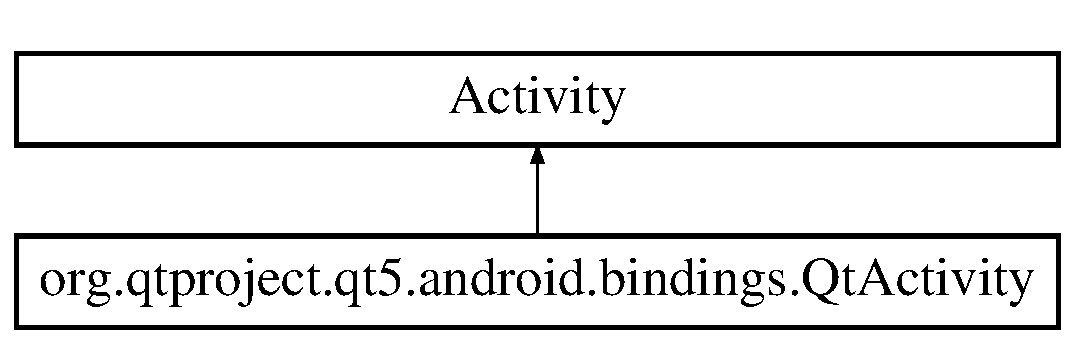
\includegraphics[height=2.000000cm]{classorg_1_1qtproject_1_1qt5_1_1android_1_1bindings_1_1_qt_activity}
\end{center}
\end{figure}
\subsection*{Public Member Functions}
\begin{DoxyCompactItemize}
\item 
\hyperlink{classorg_1_1qtproject_1_1qt5_1_1android_1_1bindings_1_1_qt_activity_ae7320eeaed590a34a648907cb524f31a}{Qt\+Activity} ()
\item 
boolean \hyperlink{classorg_1_1qtproject_1_1qt5_1_1android_1_1bindings_1_1_qt_activity_a3419f10b60670ae0fd0a222fcd684273}{dispatch\+Key\+Event} (Key\+Event event)
\item 
boolean \hyperlink{classorg_1_1qtproject_1_1qt5_1_1android_1_1bindings_1_1_qt_activity_a0222dd1edd412d5573914d8e563d8dfc}{super\+\_\+dispatch\+Key\+Event} (Key\+Event event)
\item 
boolean \hyperlink{classorg_1_1qtproject_1_1qt5_1_1android_1_1bindings_1_1_qt_activity_a7eacf9d228567bace814d7d90cc88dc1}{dispatch\+Populate\+Accessibility\+Event} (Accessibility\+Event event)
\item 
boolean \hyperlink{classorg_1_1qtproject_1_1qt5_1_1android_1_1bindings_1_1_qt_activity_a174082c8c4aa301a2a8c78ce237bca22}{super\+\_\+dispatch\+Populate\+Accessibility\+Event} (Accessibility\+Event event)
\item 
boolean \hyperlink{classorg_1_1qtproject_1_1qt5_1_1android_1_1bindings_1_1_qt_activity_a080d702cac33de4a97b4645567cf8c04}{dispatch\+Touch\+Event} (Motion\+Event ev)
\item 
boolean \hyperlink{classorg_1_1qtproject_1_1qt5_1_1android_1_1bindings_1_1_qt_activity_a8525630fd66e1d88e94f7bc9457bbd1b}{super\+\_\+dispatch\+Touch\+Event} (Motion\+Event event)
\item 
boolean \hyperlink{classorg_1_1qtproject_1_1qt5_1_1android_1_1bindings_1_1_qt_activity_ad305b6d78907e6fc4bc4fa9b77256a22}{dispatch\+Trackball\+Event} (Motion\+Event ev)
\item 
boolean \hyperlink{classorg_1_1qtproject_1_1qt5_1_1android_1_1bindings_1_1_qt_activity_a84a82b3eb7dd352d126c55272c64264a}{super\+\_\+dispatch\+Trackball\+Event} (Motion\+Event event)
\item 
void \hyperlink{classorg_1_1qtproject_1_1qt5_1_1android_1_1bindings_1_1_qt_activity_a03bf6f3f50c07592cbee97ce9ebdb315}{super\+\_\+on\+Activity\+Result} (int request\+Code, int result\+Code, Intent data)
\item 
void \hyperlink{classorg_1_1qtproject_1_1qt5_1_1android_1_1bindings_1_1_qt_activity_a03b4db053b9528617c37bab2d47fc803}{super\+\_\+on\+Apply\+Theme\+Resource} (Theme theme, int resid, boolean first)
\item 
void \hyperlink{classorg_1_1qtproject_1_1qt5_1_1android_1_1bindings_1_1_qt_activity_ac369eb38a2ea1f7a0d61c44a30d63620}{super\+\_\+on\+Child\+Title\+Changed} (Activity child\+Activity, Char\+Sequence title)
\item 
void \hyperlink{classorg_1_1qtproject_1_1qt5_1_1android_1_1bindings_1_1_qt_activity_a75ef70261caa7d4db3041147dc46c5d0}{on\+Configuration\+Changed} (Configuration new\+Config)
\item 
void \hyperlink{classorg_1_1qtproject_1_1qt5_1_1android_1_1bindings_1_1_qt_activity_a1c7f2e1b1ce16f2bfa70f38d88740565}{super\+\_\+on\+Configuration\+Changed} (Configuration new\+Config)
\item 
void \hyperlink{classorg_1_1qtproject_1_1qt5_1_1android_1_1bindings_1_1_qt_activity_a6310ffd404267a66b52dd4c3b357b560}{on\+Content\+Changed} ()
\item 
void \hyperlink{classorg_1_1qtproject_1_1qt5_1_1android_1_1bindings_1_1_qt_activity_a65dc57b70d42eb56f6bc12f7e0c49022}{super\+\_\+on\+Content\+Changed} ()
\item 
boolean \hyperlink{classorg_1_1qtproject_1_1qt5_1_1android_1_1bindings_1_1_qt_activity_a67108692da62e48e5d02b22ed3d83769}{on\+Context\+Item\+Selected} (Menu\+Item item)
\item 
boolean \hyperlink{classorg_1_1qtproject_1_1qt5_1_1android_1_1bindings_1_1_qt_activity_a7281a498436213e739110753b357c0bd}{super\+\_\+on\+Context\+Item\+Selected} (Menu\+Item item)
\item 
void \hyperlink{classorg_1_1qtproject_1_1qt5_1_1android_1_1bindings_1_1_qt_activity_a3e845800dc8fc21ff23589005d1a781c}{on\+Context\+Menu\+Closed} (Menu menu)
\item 
void \hyperlink{classorg_1_1qtproject_1_1qt5_1_1android_1_1bindings_1_1_qt_activity_a1b845060cb1ae8dde9bb8a60339b9468}{super\+\_\+on\+Context\+Menu\+Closed} (Menu menu)
\item 
void \hyperlink{classorg_1_1qtproject_1_1qt5_1_1android_1_1bindings_1_1_qt_activity_aa826639406d6f0697e0f1afcf69c748c}{on\+Create} (Bundle saved\+Instance\+State)
\item 
void \hyperlink{classorg_1_1qtproject_1_1qt5_1_1android_1_1bindings_1_1_qt_activity_a924489f96650a755cf63980f3d388e8e}{on\+Create\+Context\+Menu} (Context\+Menu menu, View v, Context\+Menu\+Info menu\+Info)
\item 
void \hyperlink{classorg_1_1qtproject_1_1qt5_1_1android_1_1bindings_1_1_qt_activity_ae235bff28fac3ae862e49a1fc52caf15}{super\+\_\+on\+Create\+Context\+Menu} (Context\+Menu menu, View v, Context\+Menu\+Info menu\+Info)
\item 
Char\+Sequence \hyperlink{classorg_1_1qtproject_1_1qt5_1_1android_1_1bindings_1_1_qt_activity_af86865337837c2c780913132b7118d69}{on\+Create\+Description} ()
\item 
Char\+Sequence \hyperlink{classorg_1_1qtproject_1_1qt5_1_1android_1_1bindings_1_1_qt_activity_a213a5e7065a1b53244d8b3642a23b2e4}{super\+\_\+on\+Create\+Description} ()
\item 
Dialog \hyperlink{classorg_1_1qtproject_1_1qt5_1_1android_1_1bindings_1_1_qt_activity_a946099e0315e24f0c40338b69e0d1cdf}{super\+\_\+on\+Create\+Dialog} (int id)
\item 
boolean \hyperlink{classorg_1_1qtproject_1_1qt5_1_1android_1_1bindings_1_1_qt_activity_a9303a2dd16e8deb7cdcf143ae6b480f4}{on\+Create\+Options\+Menu} (Menu menu)
\item 
boolean \hyperlink{classorg_1_1qtproject_1_1qt5_1_1android_1_1bindings_1_1_qt_activity_a25d0cb2383a485b28f53026ebe050dd4}{super\+\_\+on\+Create\+Options\+Menu} (Menu menu)
\item 
boolean \hyperlink{classorg_1_1qtproject_1_1qt5_1_1android_1_1bindings_1_1_qt_activity_a617b7c2c432bc9894d3c0b2490d27b41}{on\+Create\+Panel\+Menu} (int feature\+Id, Menu menu)
\item 
boolean \hyperlink{classorg_1_1qtproject_1_1qt5_1_1android_1_1bindings_1_1_qt_activity_a3d105b186ba9bf7d089699dbd5ca3c45}{super\+\_\+on\+Create\+Panel\+Menu} (int feature\+Id, Menu menu)
\item 
View \hyperlink{classorg_1_1qtproject_1_1qt5_1_1android_1_1bindings_1_1_qt_activity_aefde1977c2ccae37e5f1a927f7e9e9ee}{on\+Create\+Panel\+View} (int feature\+Id)
\item 
View \hyperlink{classorg_1_1qtproject_1_1qt5_1_1android_1_1bindings_1_1_qt_activity_ab37f48e1ce50767f29be1cebd4fc96e0}{super\+\_\+on\+Create\+Panel\+View} (int feature\+Id)
\item 
boolean \hyperlink{classorg_1_1qtproject_1_1qt5_1_1android_1_1bindings_1_1_qt_activity_a961e15fb9b7bcdc7e4310e881656e1d7}{on\+Create\+Thumbnail} (Bitmap out\+Bitmap, Canvas canvas)
\item 
boolean \hyperlink{classorg_1_1qtproject_1_1qt5_1_1android_1_1bindings_1_1_qt_activity_a2af36b766142fa45fa77623e549112ac}{super\+\_\+on\+Create\+Thumbnail} (Bitmap out\+Bitmap, Canvas canvas)
\item 
View \hyperlink{classorg_1_1qtproject_1_1qt5_1_1android_1_1bindings_1_1_qt_activity_a4f26e1f33245742068eb9b79689f69e5}{on\+Create\+View} (String name, Context context, Attribute\+Set attrs)
\item 
View \hyperlink{classorg_1_1qtproject_1_1qt5_1_1android_1_1bindings_1_1_qt_activity_a4e054eb047b9531cc8abaa75039136f2}{super\+\_\+on\+Create\+View} (String name, Context context, Attribute\+Set attrs)
\item 
boolean \hyperlink{classorg_1_1qtproject_1_1qt5_1_1android_1_1bindings_1_1_qt_activity_ac1ee5a8d6b1ed5e7757139be8d7810be}{on\+Key\+Down} (int key\+Code, Key\+Event event)
\item 
boolean \hyperlink{classorg_1_1qtproject_1_1qt5_1_1android_1_1bindings_1_1_qt_activity_af7fbc3d78f28c7599fac81499717ac8d}{super\+\_\+on\+Key\+Down} (int key\+Code, Key\+Event event)
\item 
boolean \hyperlink{classorg_1_1qtproject_1_1qt5_1_1android_1_1bindings_1_1_qt_activity_a9b41df58aada132667b9af5a8aa01aa7}{on\+Key\+Multiple} (int key\+Code, int repeat\+Count, Key\+Event event)
\item 
boolean \hyperlink{classorg_1_1qtproject_1_1qt5_1_1android_1_1bindings_1_1_qt_activity_a108ba4840f9990f299beb44cced0a45d}{super\+\_\+on\+Key\+Multiple} (int key\+Code, int repeat\+Count, Key\+Event event)
\item 
boolean \hyperlink{classorg_1_1qtproject_1_1qt5_1_1android_1_1bindings_1_1_qt_activity_ac81bcf0a973ed2f8035bc3af8ee73f78}{on\+Key\+Up} (int key\+Code, Key\+Event event)
\item 
boolean \hyperlink{classorg_1_1qtproject_1_1qt5_1_1android_1_1bindings_1_1_qt_activity_a0e236df83e1edd02ba8587199fc47e05}{super\+\_\+on\+Key\+Up} (int key\+Code, Key\+Event event)
\item 
void \hyperlink{classorg_1_1qtproject_1_1qt5_1_1android_1_1bindings_1_1_qt_activity_a60dde1c5c76102c0514119fbc9515450}{on\+Low\+Memory} ()
\item 
boolean \hyperlink{classorg_1_1qtproject_1_1qt5_1_1android_1_1bindings_1_1_qt_activity_a15f3f492aba46975a36f1ebdfbe5ba45}{on\+Menu\+Item\+Selected} (int feature\+Id, Menu\+Item item)
\item 
boolean \hyperlink{classorg_1_1qtproject_1_1qt5_1_1android_1_1bindings_1_1_qt_activity_a054b8b51a53012f32a3d30bf395c18ca}{super\+\_\+on\+Menu\+Item\+Selected} (int feature\+Id, Menu\+Item item)
\item 
boolean \hyperlink{classorg_1_1qtproject_1_1qt5_1_1android_1_1bindings_1_1_qt_activity_afa718d6a5777a519b1d513d7cbda938a}{on\+Menu\+Opened} (int feature\+Id, Menu menu)
\item 
boolean \hyperlink{classorg_1_1qtproject_1_1qt5_1_1android_1_1bindings_1_1_qt_activity_ab1719c7260a5641289249620984077bd}{super\+\_\+on\+Menu\+Opened} (int feature\+Id, Menu menu)
\item 
void \hyperlink{classorg_1_1qtproject_1_1qt5_1_1android_1_1bindings_1_1_qt_activity_afb8a02b6c2e3c8e868f8cce113f50b18}{super\+\_\+on\+New\+Intent} (Intent intent)
\item 
boolean \hyperlink{classorg_1_1qtproject_1_1qt5_1_1android_1_1bindings_1_1_qt_activity_a1062f0dfba41ba945835041b94bfe4fa}{on\+Options\+Item\+Selected} (Menu\+Item item)
\item 
boolean \hyperlink{classorg_1_1qtproject_1_1qt5_1_1android_1_1bindings_1_1_qt_activity_aab1ebb0d4fe4429af0b9e79a4a6295ad}{super\+\_\+on\+Options\+Item\+Selected} (Menu\+Item item)
\item 
void \hyperlink{classorg_1_1qtproject_1_1qt5_1_1android_1_1bindings_1_1_qt_activity_aad115f4cdaebb71916b85ac6309a83c4}{on\+Options\+Menu\+Closed} (Menu menu)
\item 
void \hyperlink{classorg_1_1qtproject_1_1qt5_1_1android_1_1bindings_1_1_qt_activity_abd8ef4d5f57f3046c3065cbe806f690b}{super\+\_\+on\+Options\+Menu\+Closed} (Menu menu)
\item 
void \hyperlink{classorg_1_1qtproject_1_1qt5_1_1android_1_1bindings_1_1_qt_activity_a2b39eac5b8b7003b20171ddce6b16e37}{on\+Panel\+Closed} (int feature\+Id, Menu menu)
\item 
void \hyperlink{classorg_1_1qtproject_1_1qt5_1_1android_1_1bindings_1_1_qt_activity_a5f9ad8da2fcebff92ef8c86583091d75}{super\+\_\+on\+Panel\+Closed} (int feature\+Id, Menu menu)
\item 
void \hyperlink{classorg_1_1qtproject_1_1qt5_1_1android_1_1bindings_1_1_qt_activity_aacc652635f4bf45e2fa182dc44e8df13}{super\+\_\+on\+Prepare\+Dialog} (int id, Dialog dialog)
\item 
boolean \hyperlink{classorg_1_1qtproject_1_1qt5_1_1android_1_1bindings_1_1_qt_activity_a71a7e747de798c51b6a385b5e8a99c61}{on\+Prepare\+Options\+Menu} (Menu menu)
\item 
boolean \hyperlink{classorg_1_1qtproject_1_1qt5_1_1android_1_1bindings_1_1_qt_activity_a9f7f63be6b9a75253b784e80bfa74f69}{super\+\_\+on\+Prepare\+Options\+Menu} (Menu menu)
\item 
boolean \hyperlink{classorg_1_1qtproject_1_1qt5_1_1android_1_1bindings_1_1_qt_activity_a668c15554849a0bce9422eb709b5cacc}{on\+Prepare\+Panel} (int feature\+Id, View view, Menu menu)
\item 
boolean \hyperlink{classorg_1_1qtproject_1_1qt5_1_1android_1_1bindings_1_1_qt_activity_ab8af6f3b5a5b4547829dc68e7c31fd86}{super\+\_\+on\+Prepare\+Panel} (int feature\+Id, View view, Menu menu)
\item 
void \hyperlink{classorg_1_1qtproject_1_1qt5_1_1android_1_1bindings_1_1_qt_activity_a73303f1db92072963fe8592eb05b0258}{super\+\_\+on\+Restore\+Instance\+State} (Bundle saved\+Instance\+State)
\item 
Object \hyperlink{classorg_1_1qtproject_1_1qt5_1_1android_1_1bindings_1_1_qt_activity_a5954d45f88dd09deba757e671de9077d}{on\+Retain\+Non\+Configuration\+Instance} ()
\item 
Object \hyperlink{classorg_1_1qtproject_1_1qt5_1_1android_1_1bindings_1_1_qt_activity_a4fa6ba75523273de5b492052f1ae06f0}{super\+\_\+on\+Retain\+Non\+Configuration\+Instance} ()
\item 
void \hyperlink{classorg_1_1qtproject_1_1qt5_1_1android_1_1bindings_1_1_qt_activity_a8fb26c42bd8d7516bf863cc5fb50e287}{super\+\_\+on\+Save\+Instance\+State} (Bundle out\+State)
\item 
boolean \hyperlink{classorg_1_1qtproject_1_1qt5_1_1android_1_1bindings_1_1_qt_activity_aa1c033b0b0bbc4cb9c193b239992fcb8}{on\+Search\+Requested} ()
\item 
boolean \hyperlink{classorg_1_1qtproject_1_1qt5_1_1android_1_1bindings_1_1_qt_activity_a41f90d68a12b8140f7b0f4c4037c2567}{super\+\_\+on\+Search\+Requested} ()
\item 
void \hyperlink{classorg_1_1qtproject_1_1qt5_1_1android_1_1bindings_1_1_qt_activity_aa3982942fa042ca69a13ffbaff0ef403}{super\+\_\+on\+Title\+Changed} (Char\+Sequence title, int color)
\item 
boolean \hyperlink{classorg_1_1qtproject_1_1qt5_1_1android_1_1bindings_1_1_qt_activity_ada200302a153c7dbab3e55b746a7a179}{on\+Touch\+Event} (Motion\+Event event)
\item 
boolean \hyperlink{classorg_1_1qtproject_1_1qt5_1_1android_1_1bindings_1_1_qt_activity_a216ec445b2cc31beac2032e38dd5e949}{super\+\_\+on\+Touch\+Event} (Motion\+Event event)
\item 
boolean \hyperlink{classorg_1_1qtproject_1_1qt5_1_1android_1_1bindings_1_1_qt_activity_a27faf58c38193faea2782ff85cedb567}{on\+Trackball\+Event} (Motion\+Event event)
\item 
boolean \hyperlink{classorg_1_1qtproject_1_1qt5_1_1android_1_1bindings_1_1_qt_activity_a4ee363f63dfde917e450b70c8880fef9}{super\+\_\+on\+Trackball\+Event} (Motion\+Event event)
\item 
void \hyperlink{classorg_1_1qtproject_1_1qt5_1_1android_1_1bindings_1_1_qt_activity_a3917d7d3ac6ab5bf31444d31b2784828}{on\+User\+Interaction} ()
\item 
void \hyperlink{classorg_1_1qtproject_1_1qt5_1_1android_1_1bindings_1_1_qt_activity_a706d78309b31669959a98b46952de75c}{super\+\_\+on\+User\+Interaction} ()
\item 
void \hyperlink{classorg_1_1qtproject_1_1qt5_1_1android_1_1bindings_1_1_qt_activity_ae71ad183d13c1bbb1fd1dccee12dde24}{super\+\_\+on\+User\+Leave\+Hint} ()
\item 
void \hyperlink{classorg_1_1qtproject_1_1qt5_1_1android_1_1bindings_1_1_qt_activity_af881fa829fb552af632f8b1bba96f351}{on\+Window\+Attributes\+Changed} (Layout\+Params params)
\item 
void \hyperlink{classorg_1_1qtproject_1_1qt5_1_1android_1_1bindings_1_1_qt_activity_aa510558df5227f66d81d6119389e7886}{super\+\_\+on\+Window\+Attributes\+Changed} (Layout\+Params params)
\item 
void \hyperlink{classorg_1_1qtproject_1_1qt5_1_1android_1_1bindings_1_1_qt_activity_ab161d356ebf5044a00182ffaf79d3437}{on\+Window\+Focus\+Changed} (boolean has\+Focus)
\item 
void \hyperlink{classorg_1_1qtproject_1_1qt5_1_1android_1_1bindings_1_1_qt_activity_a3d01ed848c426f937fe18214ff006931}{super\+\_\+on\+Window\+Focus\+Changed} (boolean has\+Focus)
\item 
void \hyperlink{classorg_1_1qtproject_1_1qt5_1_1android_1_1bindings_1_1_qt_activity_a052fd4aee0de52bcf2d8a10c5671d586}{on\+Attached\+To\+Window} ()
\item 
void \hyperlink{classorg_1_1qtproject_1_1qt5_1_1android_1_1bindings_1_1_qt_activity_a7155f32de8ac1f383e18250f28cd1f97}{super\+\_\+on\+Attached\+To\+Window} ()
\item 
void \hyperlink{classorg_1_1qtproject_1_1qt5_1_1android_1_1bindings_1_1_qt_activity_a593eeb49762865051c6348a6b98e7ff1}{on\+Back\+Pressed} ()
\item 
void \hyperlink{classorg_1_1qtproject_1_1qt5_1_1android_1_1bindings_1_1_qt_activity_a84b318d75dea61b3aa2743fb475c90da}{super\+\_\+on\+Back\+Pressed} ()
\item 
void \hyperlink{classorg_1_1qtproject_1_1qt5_1_1android_1_1bindings_1_1_qt_activity_aa7cad0cee8c325c1cbd7bb77a8a2c5ce}{on\+Detached\+From\+Window} ()
\item 
void \hyperlink{classorg_1_1qtproject_1_1qt5_1_1android_1_1bindings_1_1_qt_activity_a103cd6d406de520a7c30fa31a704ee11}{super\+\_\+on\+Detached\+From\+Window} ()
\item 
boolean \hyperlink{classorg_1_1qtproject_1_1qt5_1_1android_1_1bindings_1_1_qt_activity_ad1c024d3096ee30566b083bf35b711f4}{on\+Key\+Long\+Press} (int key\+Code, Key\+Event event)
\item 
boolean \hyperlink{classorg_1_1qtproject_1_1qt5_1_1android_1_1bindings_1_1_qt_activity_ad723f98cf99880c9467f96f73fa25878}{super\+\_\+on\+Key\+Long\+Press} (int key\+Code, Key\+Event event)
\item 
Dialog \hyperlink{classorg_1_1qtproject_1_1qt5_1_1android_1_1bindings_1_1_qt_activity_a814d7e98bb1c0355ed33457de6718bee}{super\+\_\+on\+Create\+Dialog} (int id, Bundle args)
\item 
void \hyperlink{classorg_1_1qtproject_1_1qt5_1_1android_1_1bindings_1_1_qt_activity_a385e763c50fd7d00213fe961bba46ed5}{super\+\_\+on\+Prepare\+Dialog} (int id, Dialog dialog, Bundle args)
\end{DoxyCompactItemize}
\subsection*{Public Attributes}
\begin{DoxyCompactItemize}
\item 
String \hyperlink{classorg_1_1qtproject_1_1qt5_1_1android_1_1bindings_1_1_qt_activity_a1c6754715d370c1e91160c534c54a7e7}{A\+P\+P\+L\+I\+C\+A\+T\+I\+O\+N\+\_\+\+P\+A\+R\+A\+M\+E\+T\+E\+R\+S} = null
\item 
String \hyperlink{classorg_1_1qtproject_1_1qt5_1_1android_1_1bindings_1_1_qt_activity_aa22d75fadcbc70bf4f5f668ea3300d6e}{E\+N\+V\+I\+R\+O\+N\+M\+E\+N\+T\+\_\+\+V\+A\+R\+I\+A\+B\+L\+E\+S} = \char`\"{}Q\+T\+\_\+\+U\+S\+E\+\_\+\+A\+N\+D\+R\+O\+I\+D\+\_\+\+N\+A\+T\+I\+V\+E\+\_\+\+S\+T\+Y\+L\+E=1\textbackslash{}t\+Q\+T\+\_\+\+U\+S\+E\+\_\+\+A\+N\+D\+R\+O\+I\+D\+\_\+\+N\+A\+T\+I\+V\+E\+\_\+\+D\+I\+A\+L\+O\+G\+S=1\textbackslash{}t\char`\"{}
\item 
String\mbox{[}$\,$\mbox{]} \hyperlink{classorg_1_1qtproject_1_1qt5_1_1android_1_1bindings_1_1_qt_activity_a0abec2a740bce96eec092bd1634d3a55}{Q\+T\+\_\+\+A\+N\+D\+R\+O\+I\+D\+\_\+\+T\+H\+E\+M\+E\+S} = null
\item 
String \hyperlink{classorg_1_1qtproject_1_1qt5_1_1android_1_1bindings_1_1_qt_activity_a74c21dffcaf3af985a164068c278b979}{Q\+T\+\_\+\+A\+N\+D\+R\+O\+I\+D\+\_\+\+D\+E\+F\+A\+U\+L\+T\+\_\+\+T\+H\+E\+M\+E} = null
\end{DoxyCompactItemize}
\subsection*{Protected Member Functions}
\begin{DoxyCompactItemize}
\item 
void \hyperlink{classorg_1_1qtproject_1_1qt5_1_1android_1_1bindings_1_1_qt_activity_a4e9a7c6b28384e4d5f713462207ffc41}{on\+Activity\+Result} (int request\+Code, int result\+Code, Intent data)
\item 
void \hyperlink{classorg_1_1qtproject_1_1qt5_1_1android_1_1bindings_1_1_qt_activity_acd279279e5ad448d802fa31b64a30aef}{on\+Apply\+Theme\+Resource} (Theme theme, int resid, boolean first)
\item 
void \hyperlink{classorg_1_1qtproject_1_1qt5_1_1android_1_1bindings_1_1_qt_activity_ac300f488c368a77573a3ecbf90f88b3c}{on\+Child\+Title\+Changed} (Activity child\+Activity, Char\+Sequence title)
\item 
Dialog \hyperlink{classorg_1_1qtproject_1_1qt5_1_1android_1_1bindings_1_1_qt_activity_a94b7cad79823109fd5ce75385766144b}{on\+Create\+Dialog} (int id)
\item 
void \hyperlink{classorg_1_1qtproject_1_1qt5_1_1android_1_1bindings_1_1_qt_activity_a30832553da49ca0dea222e062e21710c}{on\+Destroy} ()
\item 
void \hyperlink{classorg_1_1qtproject_1_1qt5_1_1android_1_1bindings_1_1_qt_activity_a995502b7cf803efcecc91d345b030404}{on\+New\+Intent} (Intent intent)
\item 
void \hyperlink{classorg_1_1qtproject_1_1qt5_1_1android_1_1bindings_1_1_qt_activity_a54af4563a2a1f3ea73187c2e9b9b042c}{on\+Pause} ()
\item 
void \hyperlink{classorg_1_1qtproject_1_1qt5_1_1android_1_1bindings_1_1_qt_activity_a1a206c815af224d5bf06e5c921f4fdd4}{on\+Post\+Create} (Bundle saved\+Instance\+State)
\item 
void \hyperlink{classorg_1_1qtproject_1_1qt5_1_1android_1_1bindings_1_1_qt_activity_af23189d66db86a4a4356af8481450fa1}{on\+Post\+Resume} ()
\item 
void \hyperlink{classorg_1_1qtproject_1_1qt5_1_1android_1_1bindings_1_1_qt_activity_a7c23883f7117af2b20250150e032935d}{on\+Prepare\+Dialog} (int id, Dialog dialog)
\item 
void \hyperlink{classorg_1_1qtproject_1_1qt5_1_1android_1_1bindings_1_1_qt_activity_a05a1cabee75d99161959de7575052b73}{on\+Restart} ()
\item 
void \hyperlink{classorg_1_1qtproject_1_1qt5_1_1android_1_1bindings_1_1_qt_activity_a0dd64ece074eb6909bb384a63105083b}{on\+Restore\+Instance\+State} (Bundle saved\+Instance\+State)
\item 
void \hyperlink{classorg_1_1qtproject_1_1qt5_1_1android_1_1bindings_1_1_qt_activity_a136a4d6d46f5a88c6e2b9866fa78fc64}{on\+Resume} ()
\item 
void \hyperlink{classorg_1_1qtproject_1_1qt5_1_1android_1_1bindings_1_1_qt_activity_ab32e70bfe633f137c58c82a96bf68f8f}{on\+Save\+Instance\+State} (Bundle out\+State)
\item 
void \hyperlink{classorg_1_1qtproject_1_1qt5_1_1android_1_1bindings_1_1_qt_activity_a5d86c0f23d31274741575dbf916814d1}{on\+Start} ()
\item 
void \hyperlink{classorg_1_1qtproject_1_1qt5_1_1android_1_1bindings_1_1_qt_activity_a2fa87ac6c9b33749654fb05211d7d894}{on\+Stop} ()
\item 
void \hyperlink{classorg_1_1qtproject_1_1qt5_1_1android_1_1bindings_1_1_qt_activity_ab084cdaffe2c7638d6c7e1255aecec3c}{on\+Title\+Changed} (Char\+Sequence title, int color)
\item 
void \hyperlink{classorg_1_1qtproject_1_1qt5_1_1android_1_1bindings_1_1_qt_activity_a86f980854e12f7cf5c8a91f7cbd875d7}{on\+User\+Leave\+Hint} ()
\item 
Dialog \hyperlink{classorg_1_1qtproject_1_1qt5_1_1android_1_1bindings_1_1_qt_activity_a68654d4382feda0419fd1a59792b3643}{on\+Create\+Dialog} (int id, Bundle args)
\item 
void \hyperlink{classorg_1_1qtproject_1_1qt5_1_1android_1_1bindings_1_1_qt_activity_aa4466dc136a61b68aaf83cf3a5a9827d}{on\+Prepare\+Dialog} (int id, Dialog dialog, Bundle args)
\end{DoxyCompactItemize}


\subsection{Constructor \& Destructor Documentation}
\hypertarget{classorg_1_1qtproject_1_1qt5_1_1android_1_1bindings_1_1_qt_activity_ae7320eeaed590a34a648907cb524f31a}{}\index{org\+::qtproject\+::qt5\+::android\+::bindings\+::\+Qt\+Activity@{org\+::qtproject\+::qt5\+::android\+::bindings\+::\+Qt\+Activity}!Qt\+Activity@{Qt\+Activity}}
\index{Qt\+Activity@{Qt\+Activity}!org\+::qtproject\+::qt5\+::android\+::bindings\+::\+Qt\+Activity@{org\+::qtproject\+::qt5\+::android\+::bindings\+::\+Qt\+Activity}}
\subsubsection[{Qt\+Activity}]{\setlength{\rightskip}{0pt plus 5cm}org.\+qtproject.\+qt5.\+android.\+bindings.\+Qt\+Activity.\+Qt\+Activity (
\begin{DoxyParamCaption}
{}
\end{DoxyParamCaption}
)\hspace{0.3cm}{\ttfamily [inline]}}\label{classorg_1_1qtproject_1_1qt5_1_1android_1_1bindings_1_1_qt_activity_ae7320eeaed590a34a648907cb524f31a}


\subsection{Member Function Documentation}
\hypertarget{classorg_1_1qtproject_1_1qt5_1_1android_1_1bindings_1_1_qt_activity_a3419f10b60670ae0fd0a222fcd684273}{}\index{org\+::qtproject\+::qt5\+::android\+::bindings\+::\+Qt\+Activity@{org\+::qtproject\+::qt5\+::android\+::bindings\+::\+Qt\+Activity}!dispatch\+Key\+Event@{dispatch\+Key\+Event}}
\index{dispatch\+Key\+Event@{dispatch\+Key\+Event}!org\+::qtproject\+::qt5\+::android\+::bindings\+::\+Qt\+Activity@{org\+::qtproject\+::qt5\+::android\+::bindings\+::\+Qt\+Activity}}
\subsubsection[{dispatch\+Key\+Event}]{\setlength{\rightskip}{0pt plus 5cm}boolean org.\+qtproject.\+qt5.\+android.\+bindings.\+Qt\+Activity.\+dispatch\+Key\+Event (
\begin{DoxyParamCaption}
\item[{Key\+Event}]{event}
\end{DoxyParamCaption}
)\hspace{0.3cm}{\ttfamily [inline]}}\label{classorg_1_1qtproject_1_1qt5_1_1android_1_1bindings_1_1_qt_activity_a3419f10b60670ae0fd0a222fcd684273}
\hypertarget{classorg_1_1qtproject_1_1qt5_1_1android_1_1bindings_1_1_qt_activity_a7eacf9d228567bace814d7d90cc88dc1}{}\index{org\+::qtproject\+::qt5\+::android\+::bindings\+::\+Qt\+Activity@{org\+::qtproject\+::qt5\+::android\+::bindings\+::\+Qt\+Activity}!dispatch\+Populate\+Accessibility\+Event@{dispatch\+Populate\+Accessibility\+Event}}
\index{dispatch\+Populate\+Accessibility\+Event@{dispatch\+Populate\+Accessibility\+Event}!org\+::qtproject\+::qt5\+::android\+::bindings\+::\+Qt\+Activity@{org\+::qtproject\+::qt5\+::android\+::bindings\+::\+Qt\+Activity}}
\subsubsection[{dispatch\+Populate\+Accessibility\+Event}]{\setlength{\rightskip}{0pt plus 5cm}boolean org.\+qtproject.\+qt5.\+android.\+bindings.\+Qt\+Activity.\+dispatch\+Populate\+Accessibility\+Event (
\begin{DoxyParamCaption}
\item[{Accessibility\+Event}]{event}
\end{DoxyParamCaption}
)\hspace{0.3cm}{\ttfamily [inline]}}\label{classorg_1_1qtproject_1_1qt5_1_1android_1_1bindings_1_1_qt_activity_a7eacf9d228567bace814d7d90cc88dc1}
\hypertarget{classorg_1_1qtproject_1_1qt5_1_1android_1_1bindings_1_1_qt_activity_a080d702cac33de4a97b4645567cf8c04}{}\index{org\+::qtproject\+::qt5\+::android\+::bindings\+::\+Qt\+Activity@{org\+::qtproject\+::qt5\+::android\+::bindings\+::\+Qt\+Activity}!dispatch\+Touch\+Event@{dispatch\+Touch\+Event}}
\index{dispatch\+Touch\+Event@{dispatch\+Touch\+Event}!org\+::qtproject\+::qt5\+::android\+::bindings\+::\+Qt\+Activity@{org\+::qtproject\+::qt5\+::android\+::bindings\+::\+Qt\+Activity}}
\subsubsection[{dispatch\+Touch\+Event}]{\setlength{\rightskip}{0pt plus 5cm}boolean org.\+qtproject.\+qt5.\+android.\+bindings.\+Qt\+Activity.\+dispatch\+Touch\+Event (
\begin{DoxyParamCaption}
\item[{Motion\+Event}]{ev}
\end{DoxyParamCaption}
)\hspace{0.3cm}{\ttfamily [inline]}}\label{classorg_1_1qtproject_1_1qt5_1_1android_1_1bindings_1_1_qt_activity_a080d702cac33de4a97b4645567cf8c04}
\hypertarget{classorg_1_1qtproject_1_1qt5_1_1android_1_1bindings_1_1_qt_activity_ad305b6d78907e6fc4bc4fa9b77256a22}{}\index{org\+::qtproject\+::qt5\+::android\+::bindings\+::\+Qt\+Activity@{org\+::qtproject\+::qt5\+::android\+::bindings\+::\+Qt\+Activity}!dispatch\+Trackball\+Event@{dispatch\+Trackball\+Event}}
\index{dispatch\+Trackball\+Event@{dispatch\+Trackball\+Event}!org\+::qtproject\+::qt5\+::android\+::bindings\+::\+Qt\+Activity@{org\+::qtproject\+::qt5\+::android\+::bindings\+::\+Qt\+Activity}}
\subsubsection[{dispatch\+Trackball\+Event}]{\setlength{\rightskip}{0pt plus 5cm}boolean org.\+qtproject.\+qt5.\+android.\+bindings.\+Qt\+Activity.\+dispatch\+Trackball\+Event (
\begin{DoxyParamCaption}
\item[{Motion\+Event}]{ev}
\end{DoxyParamCaption}
)\hspace{0.3cm}{\ttfamily [inline]}}\label{classorg_1_1qtproject_1_1qt5_1_1android_1_1bindings_1_1_qt_activity_ad305b6d78907e6fc4bc4fa9b77256a22}
\hypertarget{classorg_1_1qtproject_1_1qt5_1_1android_1_1bindings_1_1_qt_activity_a4e9a7c6b28384e4d5f713462207ffc41}{}\index{org\+::qtproject\+::qt5\+::android\+::bindings\+::\+Qt\+Activity@{org\+::qtproject\+::qt5\+::android\+::bindings\+::\+Qt\+Activity}!on\+Activity\+Result@{on\+Activity\+Result}}
\index{on\+Activity\+Result@{on\+Activity\+Result}!org\+::qtproject\+::qt5\+::android\+::bindings\+::\+Qt\+Activity@{org\+::qtproject\+::qt5\+::android\+::bindings\+::\+Qt\+Activity}}
\subsubsection[{on\+Activity\+Result}]{\setlength{\rightskip}{0pt plus 5cm}void org.\+qtproject.\+qt5.\+android.\+bindings.\+Qt\+Activity.\+on\+Activity\+Result (
\begin{DoxyParamCaption}
\item[{int}]{request\+Code, }
\item[{int}]{result\+Code, }
\item[{Intent}]{data}
\end{DoxyParamCaption}
)\hspace{0.3cm}{\ttfamily [inline]}, {\ttfamily [protected]}}\label{classorg_1_1qtproject_1_1qt5_1_1android_1_1bindings_1_1_qt_activity_a4e9a7c6b28384e4d5f713462207ffc41}
\hypertarget{classorg_1_1qtproject_1_1qt5_1_1android_1_1bindings_1_1_qt_activity_acd279279e5ad448d802fa31b64a30aef}{}\index{org\+::qtproject\+::qt5\+::android\+::bindings\+::\+Qt\+Activity@{org\+::qtproject\+::qt5\+::android\+::bindings\+::\+Qt\+Activity}!on\+Apply\+Theme\+Resource@{on\+Apply\+Theme\+Resource}}
\index{on\+Apply\+Theme\+Resource@{on\+Apply\+Theme\+Resource}!org\+::qtproject\+::qt5\+::android\+::bindings\+::\+Qt\+Activity@{org\+::qtproject\+::qt5\+::android\+::bindings\+::\+Qt\+Activity}}
\subsubsection[{on\+Apply\+Theme\+Resource}]{\setlength{\rightskip}{0pt plus 5cm}void org.\+qtproject.\+qt5.\+android.\+bindings.\+Qt\+Activity.\+on\+Apply\+Theme\+Resource (
\begin{DoxyParamCaption}
\item[{Theme}]{theme, }
\item[{int}]{resid, }
\item[{boolean}]{first}
\end{DoxyParamCaption}
)\hspace{0.3cm}{\ttfamily [inline]}, {\ttfamily [protected]}}\label{classorg_1_1qtproject_1_1qt5_1_1android_1_1bindings_1_1_qt_activity_acd279279e5ad448d802fa31b64a30aef}
\hypertarget{classorg_1_1qtproject_1_1qt5_1_1android_1_1bindings_1_1_qt_activity_a052fd4aee0de52bcf2d8a10c5671d586}{}\index{org\+::qtproject\+::qt5\+::android\+::bindings\+::\+Qt\+Activity@{org\+::qtproject\+::qt5\+::android\+::bindings\+::\+Qt\+Activity}!on\+Attached\+To\+Window@{on\+Attached\+To\+Window}}
\index{on\+Attached\+To\+Window@{on\+Attached\+To\+Window}!org\+::qtproject\+::qt5\+::android\+::bindings\+::\+Qt\+Activity@{org\+::qtproject\+::qt5\+::android\+::bindings\+::\+Qt\+Activity}}
\subsubsection[{on\+Attached\+To\+Window}]{\setlength{\rightskip}{0pt plus 5cm}void org.\+qtproject.\+qt5.\+android.\+bindings.\+Qt\+Activity.\+on\+Attached\+To\+Window (
\begin{DoxyParamCaption}
{}
\end{DoxyParamCaption}
)\hspace{0.3cm}{\ttfamily [inline]}}\label{classorg_1_1qtproject_1_1qt5_1_1android_1_1bindings_1_1_qt_activity_a052fd4aee0de52bcf2d8a10c5671d586}
\hypertarget{classorg_1_1qtproject_1_1qt5_1_1android_1_1bindings_1_1_qt_activity_a593eeb49762865051c6348a6b98e7ff1}{}\index{org\+::qtproject\+::qt5\+::android\+::bindings\+::\+Qt\+Activity@{org\+::qtproject\+::qt5\+::android\+::bindings\+::\+Qt\+Activity}!on\+Back\+Pressed@{on\+Back\+Pressed}}
\index{on\+Back\+Pressed@{on\+Back\+Pressed}!org\+::qtproject\+::qt5\+::android\+::bindings\+::\+Qt\+Activity@{org\+::qtproject\+::qt5\+::android\+::bindings\+::\+Qt\+Activity}}
\subsubsection[{on\+Back\+Pressed}]{\setlength{\rightskip}{0pt plus 5cm}void org.\+qtproject.\+qt5.\+android.\+bindings.\+Qt\+Activity.\+on\+Back\+Pressed (
\begin{DoxyParamCaption}
{}
\end{DoxyParamCaption}
)\hspace{0.3cm}{\ttfamily [inline]}}\label{classorg_1_1qtproject_1_1qt5_1_1android_1_1bindings_1_1_qt_activity_a593eeb49762865051c6348a6b98e7ff1}
\hypertarget{classorg_1_1qtproject_1_1qt5_1_1android_1_1bindings_1_1_qt_activity_ac300f488c368a77573a3ecbf90f88b3c}{}\index{org\+::qtproject\+::qt5\+::android\+::bindings\+::\+Qt\+Activity@{org\+::qtproject\+::qt5\+::android\+::bindings\+::\+Qt\+Activity}!on\+Child\+Title\+Changed@{on\+Child\+Title\+Changed}}
\index{on\+Child\+Title\+Changed@{on\+Child\+Title\+Changed}!org\+::qtproject\+::qt5\+::android\+::bindings\+::\+Qt\+Activity@{org\+::qtproject\+::qt5\+::android\+::bindings\+::\+Qt\+Activity}}
\subsubsection[{on\+Child\+Title\+Changed}]{\setlength{\rightskip}{0pt plus 5cm}void org.\+qtproject.\+qt5.\+android.\+bindings.\+Qt\+Activity.\+on\+Child\+Title\+Changed (
\begin{DoxyParamCaption}
\item[{Activity}]{child\+Activity, }
\item[{Char\+Sequence}]{title}
\end{DoxyParamCaption}
)\hspace{0.3cm}{\ttfamily [inline]}, {\ttfamily [protected]}}\label{classorg_1_1qtproject_1_1qt5_1_1android_1_1bindings_1_1_qt_activity_ac300f488c368a77573a3ecbf90f88b3c}
\hypertarget{classorg_1_1qtproject_1_1qt5_1_1android_1_1bindings_1_1_qt_activity_a75ef70261caa7d4db3041147dc46c5d0}{}\index{org\+::qtproject\+::qt5\+::android\+::bindings\+::\+Qt\+Activity@{org\+::qtproject\+::qt5\+::android\+::bindings\+::\+Qt\+Activity}!on\+Configuration\+Changed@{on\+Configuration\+Changed}}
\index{on\+Configuration\+Changed@{on\+Configuration\+Changed}!org\+::qtproject\+::qt5\+::android\+::bindings\+::\+Qt\+Activity@{org\+::qtproject\+::qt5\+::android\+::bindings\+::\+Qt\+Activity}}
\subsubsection[{on\+Configuration\+Changed}]{\setlength{\rightskip}{0pt plus 5cm}void org.\+qtproject.\+qt5.\+android.\+bindings.\+Qt\+Activity.\+on\+Configuration\+Changed (
\begin{DoxyParamCaption}
\item[{Configuration}]{new\+Config}
\end{DoxyParamCaption}
)\hspace{0.3cm}{\ttfamily [inline]}}\label{classorg_1_1qtproject_1_1qt5_1_1android_1_1bindings_1_1_qt_activity_a75ef70261caa7d4db3041147dc46c5d0}
\hypertarget{classorg_1_1qtproject_1_1qt5_1_1android_1_1bindings_1_1_qt_activity_a6310ffd404267a66b52dd4c3b357b560}{}\index{org\+::qtproject\+::qt5\+::android\+::bindings\+::\+Qt\+Activity@{org\+::qtproject\+::qt5\+::android\+::bindings\+::\+Qt\+Activity}!on\+Content\+Changed@{on\+Content\+Changed}}
\index{on\+Content\+Changed@{on\+Content\+Changed}!org\+::qtproject\+::qt5\+::android\+::bindings\+::\+Qt\+Activity@{org\+::qtproject\+::qt5\+::android\+::bindings\+::\+Qt\+Activity}}
\subsubsection[{on\+Content\+Changed}]{\setlength{\rightskip}{0pt plus 5cm}void org.\+qtproject.\+qt5.\+android.\+bindings.\+Qt\+Activity.\+on\+Content\+Changed (
\begin{DoxyParamCaption}
{}
\end{DoxyParamCaption}
)\hspace{0.3cm}{\ttfamily [inline]}}\label{classorg_1_1qtproject_1_1qt5_1_1android_1_1bindings_1_1_qt_activity_a6310ffd404267a66b52dd4c3b357b560}
\hypertarget{classorg_1_1qtproject_1_1qt5_1_1android_1_1bindings_1_1_qt_activity_a67108692da62e48e5d02b22ed3d83769}{}\index{org\+::qtproject\+::qt5\+::android\+::bindings\+::\+Qt\+Activity@{org\+::qtproject\+::qt5\+::android\+::bindings\+::\+Qt\+Activity}!on\+Context\+Item\+Selected@{on\+Context\+Item\+Selected}}
\index{on\+Context\+Item\+Selected@{on\+Context\+Item\+Selected}!org\+::qtproject\+::qt5\+::android\+::bindings\+::\+Qt\+Activity@{org\+::qtproject\+::qt5\+::android\+::bindings\+::\+Qt\+Activity}}
\subsubsection[{on\+Context\+Item\+Selected}]{\setlength{\rightskip}{0pt plus 5cm}boolean org.\+qtproject.\+qt5.\+android.\+bindings.\+Qt\+Activity.\+on\+Context\+Item\+Selected (
\begin{DoxyParamCaption}
\item[{Menu\+Item}]{item}
\end{DoxyParamCaption}
)\hspace{0.3cm}{\ttfamily [inline]}}\label{classorg_1_1qtproject_1_1qt5_1_1android_1_1bindings_1_1_qt_activity_a67108692da62e48e5d02b22ed3d83769}
\hypertarget{classorg_1_1qtproject_1_1qt5_1_1android_1_1bindings_1_1_qt_activity_a3e845800dc8fc21ff23589005d1a781c}{}\index{org\+::qtproject\+::qt5\+::android\+::bindings\+::\+Qt\+Activity@{org\+::qtproject\+::qt5\+::android\+::bindings\+::\+Qt\+Activity}!on\+Context\+Menu\+Closed@{on\+Context\+Menu\+Closed}}
\index{on\+Context\+Menu\+Closed@{on\+Context\+Menu\+Closed}!org\+::qtproject\+::qt5\+::android\+::bindings\+::\+Qt\+Activity@{org\+::qtproject\+::qt5\+::android\+::bindings\+::\+Qt\+Activity}}
\subsubsection[{on\+Context\+Menu\+Closed}]{\setlength{\rightskip}{0pt plus 5cm}void org.\+qtproject.\+qt5.\+android.\+bindings.\+Qt\+Activity.\+on\+Context\+Menu\+Closed (
\begin{DoxyParamCaption}
\item[{Menu}]{menu}
\end{DoxyParamCaption}
)\hspace{0.3cm}{\ttfamily [inline]}}\label{classorg_1_1qtproject_1_1qt5_1_1android_1_1bindings_1_1_qt_activity_a3e845800dc8fc21ff23589005d1a781c}
\hypertarget{classorg_1_1qtproject_1_1qt5_1_1android_1_1bindings_1_1_qt_activity_aa826639406d6f0697e0f1afcf69c748c}{}\index{org\+::qtproject\+::qt5\+::android\+::bindings\+::\+Qt\+Activity@{org\+::qtproject\+::qt5\+::android\+::bindings\+::\+Qt\+Activity}!on\+Create@{on\+Create}}
\index{on\+Create@{on\+Create}!org\+::qtproject\+::qt5\+::android\+::bindings\+::\+Qt\+Activity@{org\+::qtproject\+::qt5\+::android\+::bindings\+::\+Qt\+Activity}}
\subsubsection[{on\+Create}]{\setlength{\rightskip}{0pt plus 5cm}void org.\+qtproject.\+qt5.\+android.\+bindings.\+Qt\+Activity.\+on\+Create (
\begin{DoxyParamCaption}
\item[{Bundle}]{saved\+Instance\+State}
\end{DoxyParamCaption}
)\hspace{0.3cm}{\ttfamily [inline]}}\label{classorg_1_1qtproject_1_1qt5_1_1android_1_1bindings_1_1_qt_activity_aa826639406d6f0697e0f1afcf69c748c}
\hypertarget{classorg_1_1qtproject_1_1qt5_1_1android_1_1bindings_1_1_qt_activity_a924489f96650a755cf63980f3d388e8e}{}\index{org\+::qtproject\+::qt5\+::android\+::bindings\+::\+Qt\+Activity@{org\+::qtproject\+::qt5\+::android\+::bindings\+::\+Qt\+Activity}!on\+Create\+Context\+Menu@{on\+Create\+Context\+Menu}}
\index{on\+Create\+Context\+Menu@{on\+Create\+Context\+Menu}!org\+::qtproject\+::qt5\+::android\+::bindings\+::\+Qt\+Activity@{org\+::qtproject\+::qt5\+::android\+::bindings\+::\+Qt\+Activity}}
\subsubsection[{on\+Create\+Context\+Menu}]{\setlength{\rightskip}{0pt plus 5cm}void org.\+qtproject.\+qt5.\+android.\+bindings.\+Qt\+Activity.\+on\+Create\+Context\+Menu (
\begin{DoxyParamCaption}
\item[{Context\+Menu}]{menu, }
\item[{View}]{v, }
\item[{Context\+Menu\+Info}]{menu\+Info}
\end{DoxyParamCaption}
)\hspace{0.3cm}{\ttfamily [inline]}}\label{classorg_1_1qtproject_1_1qt5_1_1android_1_1bindings_1_1_qt_activity_a924489f96650a755cf63980f3d388e8e}
\hypertarget{classorg_1_1qtproject_1_1qt5_1_1android_1_1bindings_1_1_qt_activity_af86865337837c2c780913132b7118d69}{}\index{org\+::qtproject\+::qt5\+::android\+::bindings\+::\+Qt\+Activity@{org\+::qtproject\+::qt5\+::android\+::bindings\+::\+Qt\+Activity}!on\+Create\+Description@{on\+Create\+Description}}
\index{on\+Create\+Description@{on\+Create\+Description}!org\+::qtproject\+::qt5\+::android\+::bindings\+::\+Qt\+Activity@{org\+::qtproject\+::qt5\+::android\+::bindings\+::\+Qt\+Activity}}
\subsubsection[{on\+Create\+Description}]{\setlength{\rightskip}{0pt plus 5cm}Char\+Sequence org.\+qtproject.\+qt5.\+android.\+bindings.\+Qt\+Activity.\+on\+Create\+Description (
\begin{DoxyParamCaption}
{}
\end{DoxyParamCaption}
)\hspace{0.3cm}{\ttfamily [inline]}}\label{classorg_1_1qtproject_1_1qt5_1_1android_1_1bindings_1_1_qt_activity_af86865337837c2c780913132b7118d69}
\hypertarget{classorg_1_1qtproject_1_1qt5_1_1android_1_1bindings_1_1_qt_activity_a94b7cad79823109fd5ce75385766144b}{}\index{org\+::qtproject\+::qt5\+::android\+::bindings\+::\+Qt\+Activity@{org\+::qtproject\+::qt5\+::android\+::bindings\+::\+Qt\+Activity}!on\+Create\+Dialog@{on\+Create\+Dialog}}
\index{on\+Create\+Dialog@{on\+Create\+Dialog}!org\+::qtproject\+::qt5\+::android\+::bindings\+::\+Qt\+Activity@{org\+::qtproject\+::qt5\+::android\+::bindings\+::\+Qt\+Activity}}
\subsubsection[{on\+Create\+Dialog}]{\setlength{\rightskip}{0pt plus 5cm}Dialog org.\+qtproject.\+qt5.\+android.\+bindings.\+Qt\+Activity.\+on\+Create\+Dialog (
\begin{DoxyParamCaption}
\item[{int}]{id}
\end{DoxyParamCaption}
)\hspace{0.3cm}{\ttfamily [inline]}, {\ttfamily [protected]}}\label{classorg_1_1qtproject_1_1qt5_1_1android_1_1bindings_1_1_qt_activity_a94b7cad79823109fd5ce75385766144b}
\hypertarget{classorg_1_1qtproject_1_1qt5_1_1android_1_1bindings_1_1_qt_activity_a68654d4382feda0419fd1a59792b3643}{}\index{org\+::qtproject\+::qt5\+::android\+::bindings\+::\+Qt\+Activity@{org\+::qtproject\+::qt5\+::android\+::bindings\+::\+Qt\+Activity}!on\+Create\+Dialog@{on\+Create\+Dialog}}
\index{on\+Create\+Dialog@{on\+Create\+Dialog}!org\+::qtproject\+::qt5\+::android\+::bindings\+::\+Qt\+Activity@{org\+::qtproject\+::qt5\+::android\+::bindings\+::\+Qt\+Activity}}
\subsubsection[{on\+Create\+Dialog}]{\setlength{\rightskip}{0pt plus 5cm}Dialog org.\+qtproject.\+qt5.\+android.\+bindings.\+Qt\+Activity.\+on\+Create\+Dialog (
\begin{DoxyParamCaption}
\item[{int}]{id, }
\item[{Bundle}]{args}
\end{DoxyParamCaption}
)\hspace{0.3cm}{\ttfamily [inline]}, {\ttfamily [protected]}}\label{classorg_1_1qtproject_1_1qt5_1_1android_1_1bindings_1_1_qt_activity_a68654d4382feda0419fd1a59792b3643}
\hypertarget{classorg_1_1qtproject_1_1qt5_1_1android_1_1bindings_1_1_qt_activity_a9303a2dd16e8deb7cdcf143ae6b480f4}{}\index{org\+::qtproject\+::qt5\+::android\+::bindings\+::\+Qt\+Activity@{org\+::qtproject\+::qt5\+::android\+::bindings\+::\+Qt\+Activity}!on\+Create\+Options\+Menu@{on\+Create\+Options\+Menu}}
\index{on\+Create\+Options\+Menu@{on\+Create\+Options\+Menu}!org\+::qtproject\+::qt5\+::android\+::bindings\+::\+Qt\+Activity@{org\+::qtproject\+::qt5\+::android\+::bindings\+::\+Qt\+Activity}}
\subsubsection[{on\+Create\+Options\+Menu}]{\setlength{\rightskip}{0pt plus 5cm}boolean org.\+qtproject.\+qt5.\+android.\+bindings.\+Qt\+Activity.\+on\+Create\+Options\+Menu (
\begin{DoxyParamCaption}
\item[{Menu}]{menu}
\end{DoxyParamCaption}
)\hspace{0.3cm}{\ttfamily [inline]}}\label{classorg_1_1qtproject_1_1qt5_1_1android_1_1bindings_1_1_qt_activity_a9303a2dd16e8deb7cdcf143ae6b480f4}
\hypertarget{classorg_1_1qtproject_1_1qt5_1_1android_1_1bindings_1_1_qt_activity_a617b7c2c432bc9894d3c0b2490d27b41}{}\index{org\+::qtproject\+::qt5\+::android\+::bindings\+::\+Qt\+Activity@{org\+::qtproject\+::qt5\+::android\+::bindings\+::\+Qt\+Activity}!on\+Create\+Panel\+Menu@{on\+Create\+Panel\+Menu}}
\index{on\+Create\+Panel\+Menu@{on\+Create\+Panel\+Menu}!org\+::qtproject\+::qt5\+::android\+::bindings\+::\+Qt\+Activity@{org\+::qtproject\+::qt5\+::android\+::bindings\+::\+Qt\+Activity}}
\subsubsection[{on\+Create\+Panel\+Menu}]{\setlength{\rightskip}{0pt plus 5cm}boolean org.\+qtproject.\+qt5.\+android.\+bindings.\+Qt\+Activity.\+on\+Create\+Panel\+Menu (
\begin{DoxyParamCaption}
\item[{int}]{feature\+Id, }
\item[{Menu}]{menu}
\end{DoxyParamCaption}
)\hspace{0.3cm}{\ttfamily [inline]}}\label{classorg_1_1qtproject_1_1qt5_1_1android_1_1bindings_1_1_qt_activity_a617b7c2c432bc9894d3c0b2490d27b41}
\hypertarget{classorg_1_1qtproject_1_1qt5_1_1android_1_1bindings_1_1_qt_activity_aefde1977c2ccae37e5f1a927f7e9e9ee}{}\index{org\+::qtproject\+::qt5\+::android\+::bindings\+::\+Qt\+Activity@{org\+::qtproject\+::qt5\+::android\+::bindings\+::\+Qt\+Activity}!on\+Create\+Panel\+View@{on\+Create\+Panel\+View}}
\index{on\+Create\+Panel\+View@{on\+Create\+Panel\+View}!org\+::qtproject\+::qt5\+::android\+::bindings\+::\+Qt\+Activity@{org\+::qtproject\+::qt5\+::android\+::bindings\+::\+Qt\+Activity}}
\subsubsection[{on\+Create\+Panel\+View}]{\setlength{\rightskip}{0pt plus 5cm}View org.\+qtproject.\+qt5.\+android.\+bindings.\+Qt\+Activity.\+on\+Create\+Panel\+View (
\begin{DoxyParamCaption}
\item[{int}]{feature\+Id}
\end{DoxyParamCaption}
)\hspace{0.3cm}{\ttfamily [inline]}}\label{classorg_1_1qtproject_1_1qt5_1_1android_1_1bindings_1_1_qt_activity_aefde1977c2ccae37e5f1a927f7e9e9ee}
\hypertarget{classorg_1_1qtproject_1_1qt5_1_1android_1_1bindings_1_1_qt_activity_a961e15fb9b7bcdc7e4310e881656e1d7}{}\index{org\+::qtproject\+::qt5\+::android\+::bindings\+::\+Qt\+Activity@{org\+::qtproject\+::qt5\+::android\+::bindings\+::\+Qt\+Activity}!on\+Create\+Thumbnail@{on\+Create\+Thumbnail}}
\index{on\+Create\+Thumbnail@{on\+Create\+Thumbnail}!org\+::qtproject\+::qt5\+::android\+::bindings\+::\+Qt\+Activity@{org\+::qtproject\+::qt5\+::android\+::bindings\+::\+Qt\+Activity}}
\subsubsection[{on\+Create\+Thumbnail}]{\setlength{\rightskip}{0pt plus 5cm}boolean org.\+qtproject.\+qt5.\+android.\+bindings.\+Qt\+Activity.\+on\+Create\+Thumbnail (
\begin{DoxyParamCaption}
\item[{Bitmap}]{out\+Bitmap, }
\item[{Canvas}]{canvas}
\end{DoxyParamCaption}
)\hspace{0.3cm}{\ttfamily [inline]}}\label{classorg_1_1qtproject_1_1qt5_1_1android_1_1bindings_1_1_qt_activity_a961e15fb9b7bcdc7e4310e881656e1d7}
\hypertarget{classorg_1_1qtproject_1_1qt5_1_1android_1_1bindings_1_1_qt_activity_a4f26e1f33245742068eb9b79689f69e5}{}\index{org\+::qtproject\+::qt5\+::android\+::bindings\+::\+Qt\+Activity@{org\+::qtproject\+::qt5\+::android\+::bindings\+::\+Qt\+Activity}!on\+Create\+View@{on\+Create\+View}}
\index{on\+Create\+View@{on\+Create\+View}!org\+::qtproject\+::qt5\+::android\+::bindings\+::\+Qt\+Activity@{org\+::qtproject\+::qt5\+::android\+::bindings\+::\+Qt\+Activity}}
\subsubsection[{on\+Create\+View}]{\setlength{\rightskip}{0pt plus 5cm}View org.\+qtproject.\+qt5.\+android.\+bindings.\+Qt\+Activity.\+on\+Create\+View (
\begin{DoxyParamCaption}
\item[{String}]{name, }
\item[{Context}]{context, }
\item[{Attribute\+Set}]{attrs}
\end{DoxyParamCaption}
)\hspace{0.3cm}{\ttfamily [inline]}}\label{classorg_1_1qtproject_1_1qt5_1_1android_1_1bindings_1_1_qt_activity_a4f26e1f33245742068eb9b79689f69e5}
\hypertarget{classorg_1_1qtproject_1_1qt5_1_1android_1_1bindings_1_1_qt_activity_a30832553da49ca0dea222e062e21710c}{}\index{org\+::qtproject\+::qt5\+::android\+::bindings\+::\+Qt\+Activity@{org\+::qtproject\+::qt5\+::android\+::bindings\+::\+Qt\+Activity}!on\+Destroy@{on\+Destroy}}
\index{on\+Destroy@{on\+Destroy}!org\+::qtproject\+::qt5\+::android\+::bindings\+::\+Qt\+Activity@{org\+::qtproject\+::qt5\+::android\+::bindings\+::\+Qt\+Activity}}
\subsubsection[{on\+Destroy}]{\setlength{\rightskip}{0pt plus 5cm}void org.\+qtproject.\+qt5.\+android.\+bindings.\+Qt\+Activity.\+on\+Destroy (
\begin{DoxyParamCaption}
{}
\end{DoxyParamCaption}
)\hspace{0.3cm}{\ttfamily [inline]}, {\ttfamily [protected]}}\label{classorg_1_1qtproject_1_1qt5_1_1android_1_1bindings_1_1_qt_activity_a30832553da49ca0dea222e062e21710c}
\hypertarget{classorg_1_1qtproject_1_1qt5_1_1android_1_1bindings_1_1_qt_activity_aa7cad0cee8c325c1cbd7bb77a8a2c5ce}{}\index{org\+::qtproject\+::qt5\+::android\+::bindings\+::\+Qt\+Activity@{org\+::qtproject\+::qt5\+::android\+::bindings\+::\+Qt\+Activity}!on\+Detached\+From\+Window@{on\+Detached\+From\+Window}}
\index{on\+Detached\+From\+Window@{on\+Detached\+From\+Window}!org\+::qtproject\+::qt5\+::android\+::bindings\+::\+Qt\+Activity@{org\+::qtproject\+::qt5\+::android\+::bindings\+::\+Qt\+Activity}}
\subsubsection[{on\+Detached\+From\+Window}]{\setlength{\rightskip}{0pt plus 5cm}void org.\+qtproject.\+qt5.\+android.\+bindings.\+Qt\+Activity.\+on\+Detached\+From\+Window (
\begin{DoxyParamCaption}
{}
\end{DoxyParamCaption}
)\hspace{0.3cm}{\ttfamily [inline]}}\label{classorg_1_1qtproject_1_1qt5_1_1android_1_1bindings_1_1_qt_activity_aa7cad0cee8c325c1cbd7bb77a8a2c5ce}
\hypertarget{classorg_1_1qtproject_1_1qt5_1_1android_1_1bindings_1_1_qt_activity_ac1ee5a8d6b1ed5e7757139be8d7810be}{}\index{org\+::qtproject\+::qt5\+::android\+::bindings\+::\+Qt\+Activity@{org\+::qtproject\+::qt5\+::android\+::bindings\+::\+Qt\+Activity}!on\+Key\+Down@{on\+Key\+Down}}
\index{on\+Key\+Down@{on\+Key\+Down}!org\+::qtproject\+::qt5\+::android\+::bindings\+::\+Qt\+Activity@{org\+::qtproject\+::qt5\+::android\+::bindings\+::\+Qt\+Activity}}
\subsubsection[{on\+Key\+Down}]{\setlength{\rightskip}{0pt plus 5cm}boolean org.\+qtproject.\+qt5.\+android.\+bindings.\+Qt\+Activity.\+on\+Key\+Down (
\begin{DoxyParamCaption}
\item[{int}]{key\+Code, }
\item[{Key\+Event}]{event}
\end{DoxyParamCaption}
)\hspace{0.3cm}{\ttfamily [inline]}}\label{classorg_1_1qtproject_1_1qt5_1_1android_1_1bindings_1_1_qt_activity_ac1ee5a8d6b1ed5e7757139be8d7810be}
\hypertarget{classorg_1_1qtproject_1_1qt5_1_1android_1_1bindings_1_1_qt_activity_ad1c024d3096ee30566b083bf35b711f4}{}\index{org\+::qtproject\+::qt5\+::android\+::bindings\+::\+Qt\+Activity@{org\+::qtproject\+::qt5\+::android\+::bindings\+::\+Qt\+Activity}!on\+Key\+Long\+Press@{on\+Key\+Long\+Press}}
\index{on\+Key\+Long\+Press@{on\+Key\+Long\+Press}!org\+::qtproject\+::qt5\+::android\+::bindings\+::\+Qt\+Activity@{org\+::qtproject\+::qt5\+::android\+::bindings\+::\+Qt\+Activity}}
\subsubsection[{on\+Key\+Long\+Press}]{\setlength{\rightskip}{0pt plus 5cm}boolean org.\+qtproject.\+qt5.\+android.\+bindings.\+Qt\+Activity.\+on\+Key\+Long\+Press (
\begin{DoxyParamCaption}
\item[{int}]{key\+Code, }
\item[{Key\+Event}]{event}
\end{DoxyParamCaption}
)\hspace{0.3cm}{\ttfamily [inline]}}\label{classorg_1_1qtproject_1_1qt5_1_1android_1_1bindings_1_1_qt_activity_ad1c024d3096ee30566b083bf35b711f4}
\hypertarget{classorg_1_1qtproject_1_1qt5_1_1android_1_1bindings_1_1_qt_activity_a9b41df58aada132667b9af5a8aa01aa7}{}\index{org\+::qtproject\+::qt5\+::android\+::bindings\+::\+Qt\+Activity@{org\+::qtproject\+::qt5\+::android\+::bindings\+::\+Qt\+Activity}!on\+Key\+Multiple@{on\+Key\+Multiple}}
\index{on\+Key\+Multiple@{on\+Key\+Multiple}!org\+::qtproject\+::qt5\+::android\+::bindings\+::\+Qt\+Activity@{org\+::qtproject\+::qt5\+::android\+::bindings\+::\+Qt\+Activity}}
\subsubsection[{on\+Key\+Multiple}]{\setlength{\rightskip}{0pt plus 5cm}boolean org.\+qtproject.\+qt5.\+android.\+bindings.\+Qt\+Activity.\+on\+Key\+Multiple (
\begin{DoxyParamCaption}
\item[{int}]{key\+Code, }
\item[{int}]{repeat\+Count, }
\item[{Key\+Event}]{event}
\end{DoxyParamCaption}
)\hspace{0.3cm}{\ttfamily [inline]}}\label{classorg_1_1qtproject_1_1qt5_1_1android_1_1bindings_1_1_qt_activity_a9b41df58aada132667b9af5a8aa01aa7}
\hypertarget{classorg_1_1qtproject_1_1qt5_1_1android_1_1bindings_1_1_qt_activity_ac81bcf0a973ed2f8035bc3af8ee73f78}{}\index{org\+::qtproject\+::qt5\+::android\+::bindings\+::\+Qt\+Activity@{org\+::qtproject\+::qt5\+::android\+::bindings\+::\+Qt\+Activity}!on\+Key\+Up@{on\+Key\+Up}}
\index{on\+Key\+Up@{on\+Key\+Up}!org\+::qtproject\+::qt5\+::android\+::bindings\+::\+Qt\+Activity@{org\+::qtproject\+::qt5\+::android\+::bindings\+::\+Qt\+Activity}}
\subsubsection[{on\+Key\+Up}]{\setlength{\rightskip}{0pt plus 5cm}boolean org.\+qtproject.\+qt5.\+android.\+bindings.\+Qt\+Activity.\+on\+Key\+Up (
\begin{DoxyParamCaption}
\item[{int}]{key\+Code, }
\item[{Key\+Event}]{event}
\end{DoxyParamCaption}
)\hspace{0.3cm}{\ttfamily [inline]}}\label{classorg_1_1qtproject_1_1qt5_1_1android_1_1bindings_1_1_qt_activity_ac81bcf0a973ed2f8035bc3af8ee73f78}
\hypertarget{classorg_1_1qtproject_1_1qt5_1_1android_1_1bindings_1_1_qt_activity_a60dde1c5c76102c0514119fbc9515450}{}\index{org\+::qtproject\+::qt5\+::android\+::bindings\+::\+Qt\+Activity@{org\+::qtproject\+::qt5\+::android\+::bindings\+::\+Qt\+Activity}!on\+Low\+Memory@{on\+Low\+Memory}}
\index{on\+Low\+Memory@{on\+Low\+Memory}!org\+::qtproject\+::qt5\+::android\+::bindings\+::\+Qt\+Activity@{org\+::qtproject\+::qt5\+::android\+::bindings\+::\+Qt\+Activity}}
\subsubsection[{on\+Low\+Memory}]{\setlength{\rightskip}{0pt plus 5cm}void org.\+qtproject.\+qt5.\+android.\+bindings.\+Qt\+Activity.\+on\+Low\+Memory (
\begin{DoxyParamCaption}
{}
\end{DoxyParamCaption}
)\hspace{0.3cm}{\ttfamily [inline]}}\label{classorg_1_1qtproject_1_1qt5_1_1android_1_1bindings_1_1_qt_activity_a60dde1c5c76102c0514119fbc9515450}
\hypertarget{classorg_1_1qtproject_1_1qt5_1_1android_1_1bindings_1_1_qt_activity_a15f3f492aba46975a36f1ebdfbe5ba45}{}\index{org\+::qtproject\+::qt5\+::android\+::bindings\+::\+Qt\+Activity@{org\+::qtproject\+::qt5\+::android\+::bindings\+::\+Qt\+Activity}!on\+Menu\+Item\+Selected@{on\+Menu\+Item\+Selected}}
\index{on\+Menu\+Item\+Selected@{on\+Menu\+Item\+Selected}!org\+::qtproject\+::qt5\+::android\+::bindings\+::\+Qt\+Activity@{org\+::qtproject\+::qt5\+::android\+::bindings\+::\+Qt\+Activity}}
\subsubsection[{on\+Menu\+Item\+Selected}]{\setlength{\rightskip}{0pt plus 5cm}boolean org.\+qtproject.\+qt5.\+android.\+bindings.\+Qt\+Activity.\+on\+Menu\+Item\+Selected (
\begin{DoxyParamCaption}
\item[{int}]{feature\+Id, }
\item[{Menu\+Item}]{item}
\end{DoxyParamCaption}
)\hspace{0.3cm}{\ttfamily [inline]}}\label{classorg_1_1qtproject_1_1qt5_1_1android_1_1bindings_1_1_qt_activity_a15f3f492aba46975a36f1ebdfbe5ba45}
\hypertarget{classorg_1_1qtproject_1_1qt5_1_1android_1_1bindings_1_1_qt_activity_afa718d6a5777a519b1d513d7cbda938a}{}\index{org\+::qtproject\+::qt5\+::android\+::bindings\+::\+Qt\+Activity@{org\+::qtproject\+::qt5\+::android\+::bindings\+::\+Qt\+Activity}!on\+Menu\+Opened@{on\+Menu\+Opened}}
\index{on\+Menu\+Opened@{on\+Menu\+Opened}!org\+::qtproject\+::qt5\+::android\+::bindings\+::\+Qt\+Activity@{org\+::qtproject\+::qt5\+::android\+::bindings\+::\+Qt\+Activity}}
\subsubsection[{on\+Menu\+Opened}]{\setlength{\rightskip}{0pt plus 5cm}boolean org.\+qtproject.\+qt5.\+android.\+bindings.\+Qt\+Activity.\+on\+Menu\+Opened (
\begin{DoxyParamCaption}
\item[{int}]{feature\+Id, }
\item[{Menu}]{menu}
\end{DoxyParamCaption}
)\hspace{0.3cm}{\ttfamily [inline]}}\label{classorg_1_1qtproject_1_1qt5_1_1android_1_1bindings_1_1_qt_activity_afa718d6a5777a519b1d513d7cbda938a}
\hypertarget{classorg_1_1qtproject_1_1qt5_1_1android_1_1bindings_1_1_qt_activity_a995502b7cf803efcecc91d345b030404}{}\index{org\+::qtproject\+::qt5\+::android\+::bindings\+::\+Qt\+Activity@{org\+::qtproject\+::qt5\+::android\+::bindings\+::\+Qt\+Activity}!on\+New\+Intent@{on\+New\+Intent}}
\index{on\+New\+Intent@{on\+New\+Intent}!org\+::qtproject\+::qt5\+::android\+::bindings\+::\+Qt\+Activity@{org\+::qtproject\+::qt5\+::android\+::bindings\+::\+Qt\+Activity}}
\subsubsection[{on\+New\+Intent}]{\setlength{\rightskip}{0pt plus 5cm}void org.\+qtproject.\+qt5.\+android.\+bindings.\+Qt\+Activity.\+on\+New\+Intent (
\begin{DoxyParamCaption}
\item[{Intent}]{intent}
\end{DoxyParamCaption}
)\hspace{0.3cm}{\ttfamily [inline]}, {\ttfamily [protected]}}\label{classorg_1_1qtproject_1_1qt5_1_1android_1_1bindings_1_1_qt_activity_a995502b7cf803efcecc91d345b030404}
\hypertarget{classorg_1_1qtproject_1_1qt5_1_1android_1_1bindings_1_1_qt_activity_a1062f0dfba41ba945835041b94bfe4fa}{}\index{org\+::qtproject\+::qt5\+::android\+::bindings\+::\+Qt\+Activity@{org\+::qtproject\+::qt5\+::android\+::bindings\+::\+Qt\+Activity}!on\+Options\+Item\+Selected@{on\+Options\+Item\+Selected}}
\index{on\+Options\+Item\+Selected@{on\+Options\+Item\+Selected}!org\+::qtproject\+::qt5\+::android\+::bindings\+::\+Qt\+Activity@{org\+::qtproject\+::qt5\+::android\+::bindings\+::\+Qt\+Activity}}
\subsubsection[{on\+Options\+Item\+Selected}]{\setlength{\rightskip}{0pt plus 5cm}boolean org.\+qtproject.\+qt5.\+android.\+bindings.\+Qt\+Activity.\+on\+Options\+Item\+Selected (
\begin{DoxyParamCaption}
\item[{Menu\+Item}]{item}
\end{DoxyParamCaption}
)\hspace{0.3cm}{\ttfamily [inline]}}\label{classorg_1_1qtproject_1_1qt5_1_1android_1_1bindings_1_1_qt_activity_a1062f0dfba41ba945835041b94bfe4fa}
\hypertarget{classorg_1_1qtproject_1_1qt5_1_1android_1_1bindings_1_1_qt_activity_aad115f4cdaebb71916b85ac6309a83c4}{}\index{org\+::qtproject\+::qt5\+::android\+::bindings\+::\+Qt\+Activity@{org\+::qtproject\+::qt5\+::android\+::bindings\+::\+Qt\+Activity}!on\+Options\+Menu\+Closed@{on\+Options\+Menu\+Closed}}
\index{on\+Options\+Menu\+Closed@{on\+Options\+Menu\+Closed}!org\+::qtproject\+::qt5\+::android\+::bindings\+::\+Qt\+Activity@{org\+::qtproject\+::qt5\+::android\+::bindings\+::\+Qt\+Activity}}
\subsubsection[{on\+Options\+Menu\+Closed}]{\setlength{\rightskip}{0pt plus 5cm}void org.\+qtproject.\+qt5.\+android.\+bindings.\+Qt\+Activity.\+on\+Options\+Menu\+Closed (
\begin{DoxyParamCaption}
\item[{Menu}]{menu}
\end{DoxyParamCaption}
)\hspace{0.3cm}{\ttfamily [inline]}}\label{classorg_1_1qtproject_1_1qt5_1_1android_1_1bindings_1_1_qt_activity_aad115f4cdaebb71916b85ac6309a83c4}
\hypertarget{classorg_1_1qtproject_1_1qt5_1_1android_1_1bindings_1_1_qt_activity_a2b39eac5b8b7003b20171ddce6b16e37}{}\index{org\+::qtproject\+::qt5\+::android\+::bindings\+::\+Qt\+Activity@{org\+::qtproject\+::qt5\+::android\+::bindings\+::\+Qt\+Activity}!on\+Panel\+Closed@{on\+Panel\+Closed}}
\index{on\+Panel\+Closed@{on\+Panel\+Closed}!org\+::qtproject\+::qt5\+::android\+::bindings\+::\+Qt\+Activity@{org\+::qtproject\+::qt5\+::android\+::bindings\+::\+Qt\+Activity}}
\subsubsection[{on\+Panel\+Closed}]{\setlength{\rightskip}{0pt plus 5cm}void org.\+qtproject.\+qt5.\+android.\+bindings.\+Qt\+Activity.\+on\+Panel\+Closed (
\begin{DoxyParamCaption}
\item[{int}]{feature\+Id, }
\item[{Menu}]{menu}
\end{DoxyParamCaption}
)\hspace{0.3cm}{\ttfamily [inline]}}\label{classorg_1_1qtproject_1_1qt5_1_1android_1_1bindings_1_1_qt_activity_a2b39eac5b8b7003b20171ddce6b16e37}
\hypertarget{classorg_1_1qtproject_1_1qt5_1_1android_1_1bindings_1_1_qt_activity_a54af4563a2a1f3ea73187c2e9b9b042c}{}\index{org\+::qtproject\+::qt5\+::android\+::bindings\+::\+Qt\+Activity@{org\+::qtproject\+::qt5\+::android\+::bindings\+::\+Qt\+Activity}!on\+Pause@{on\+Pause}}
\index{on\+Pause@{on\+Pause}!org\+::qtproject\+::qt5\+::android\+::bindings\+::\+Qt\+Activity@{org\+::qtproject\+::qt5\+::android\+::bindings\+::\+Qt\+Activity}}
\subsubsection[{on\+Pause}]{\setlength{\rightskip}{0pt plus 5cm}void org.\+qtproject.\+qt5.\+android.\+bindings.\+Qt\+Activity.\+on\+Pause (
\begin{DoxyParamCaption}
{}
\end{DoxyParamCaption}
)\hspace{0.3cm}{\ttfamily [inline]}, {\ttfamily [protected]}}\label{classorg_1_1qtproject_1_1qt5_1_1android_1_1bindings_1_1_qt_activity_a54af4563a2a1f3ea73187c2e9b9b042c}
\hypertarget{classorg_1_1qtproject_1_1qt5_1_1android_1_1bindings_1_1_qt_activity_a1a206c815af224d5bf06e5c921f4fdd4}{}\index{org\+::qtproject\+::qt5\+::android\+::bindings\+::\+Qt\+Activity@{org\+::qtproject\+::qt5\+::android\+::bindings\+::\+Qt\+Activity}!on\+Post\+Create@{on\+Post\+Create}}
\index{on\+Post\+Create@{on\+Post\+Create}!org\+::qtproject\+::qt5\+::android\+::bindings\+::\+Qt\+Activity@{org\+::qtproject\+::qt5\+::android\+::bindings\+::\+Qt\+Activity}}
\subsubsection[{on\+Post\+Create}]{\setlength{\rightskip}{0pt plus 5cm}void org.\+qtproject.\+qt5.\+android.\+bindings.\+Qt\+Activity.\+on\+Post\+Create (
\begin{DoxyParamCaption}
\item[{Bundle}]{saved\+Instance\+State}
\end{DoxyParamCaption}
)\hspace{0.3cm}{\ttfamily [inline]}, {\ttfamily [protected]}}\label{classorg_1_1qtproject_1_1qt5_1_1android_1_1bindings_1_1_qt_activity_a1a206c815af224d5bf06e5c921f4fdd4}
\hypertarget{classorg_1_1qtproject_1_1qt5_1_1android_1_1bindings_1_1_qt_activity_af23189d66db86a4a4356af8481450fa1}{}\index{org\+::qtproject\+::qt5\+::android\+::bindings\+::\+Qt\+Activity@{org\+::qtproject\+::qt5\+::android\+::bindings\+::\+Qt\+Activity}!on\+Post\+Resume@{on\+Post\+Resume}}
\index{on\+Post\+Resume@{on\+Post\+Resume}!org\+::qtproject\+::qt5\+::android\+::bindings\+::\+Qt\+Activity@{org\+::qtproject\+::qt5\+::android\+::bindings\+::\+Qt\+Activity}}
\subsubsection[{on\+Post\+Resume}]{\setlength{\rightskip}{0pt plus 5cm}void org.\+qtproject.\+qt5.\+android.\+bindings.\+Qt\+Activity.\+on\+Post\+Resume (
\begin{DoxyParamCaption}
{}
\end{DoxyParamCaption}
)\hspace{0.3cm}{\ttfamily [inline]}, {\ttfamily [protected]}}\label{classorg_1_1qtproject_1_1qt5_1_1android_1_1bindings_1_1_qt_activity_af23189d66db86a4a4356af8481450fa1}
\hypertarget{classorg_1_1qtproject_1_1qt5_1_1android_1_1bindings_1_1_qt_activity_a7c23883f7117af2b20250150e032935d}{}\index{org\+::qtproject\+::qt5\+::android\+::bindings\+::\+Qt\+Activity@{org\+::qtproject\+::qt5\+::android\+::bindings\+::\+Qt\+Activity}!on\+Prepare\+Dialog@{on\+Prepare\+Dialog}}
\index{on\+Prepare\+Dialog@{on\+Prepare\+Dialog}!org\+::qtproject\+::qt5\+::android\+::bindings\+::\+Qt\+Activity@{org\+::qtproject\+::qt5\+::android\+::bindings\+::\+Qt\+Activity}}
\subsubsection[{on\+Prepare\+Dialog}]{\setlength{\rightskip}{0pt plus 5cm}void org.\+qtproject.\+qt5.\+android.\+bindings.\+Qt\+Activity.\+on\+Prepare\+Dialog (
\begin{DoxyParamCaption}
\item[{int}]{id, }
\item[{Dialog}]{dialog}
\end{DoxyParamCaption}
)\hspace{0.3cm}{\ttfamily [inline]}, {\ttfamily [protected]}}\label{classorg_1_1qtproject_1_1qt5_1_1android_1_1bindings_1_1_qt_activity_a7c23883f7117af2b20250150e032935d}
\hypertarget{classorg_1_1qtproject_1_1qt5_1_1android_1_1bindings_1_1_qt_activity_aa4466dc136a61b68aaf83cf3a5a9827d}{}\index{org\+::qtproject\+::qt5\+::android\+::bindings\+::\+Qt\+Activity@{org\+::qtproject\+::qt5\+::android\+::bindings\+::\+Qt\+Activity}!on\+Prepare\+Dialog@{on\+Prepare\+Dialog}}
\index{on\+Prepare\+Dialog@{on\+Prepare\+Dialog}!org\+::qtproject\+::qt5\+::android\+::bindings\+::\+Qt\+Activity@{org\+::qtproject\+::qt5\+::android\+::bindings\+::\+Qt\+Activity}}
\subsubsection[{on\+Prepare\+Dialog}]{\setlength{\rightskip}{0pt plus 5cm}void org.\+qtproject.\+qt5.\+android.\+bindings.\+Qt\+Activity.\+on\+Prepare\+Dialog (
\begin{DoxyParamCaption}
\item[{int}]{id, }
\item[{Dialog}]{dialog, }
\item[{Bundle}]{args}
\end{DoxyParamCaption}
)\hspace{0.3cm}{\ttfamily [inline]}, {\ttfamily [protected]}}\label{classorg_1_1qtproject_1_1qt5_1_1android_1_1bindings_1_1_qt_activity_aa4466dc136a61b68aaf83cf3a5a9827d}
\hypertarget{classorg_1_1qtproject_1_1qt5_1_1android_1_1bindings_1_1_qt_activity_a71a7e747de798c51b6a385b5e8a99c61}{}\index{org\+::qtproject\+::qt5\+::android\+::bindings\+::\+Qt\+Activity@{org\+::qtproject\+::qt5\+::android\+::bindings\+::\+Qt\+Activity}!on\+Prepare\+Options\+Menu@{on\+Prepare\+Options\+Menu}}
\index{on\+Prepare\+Options\+Menu@{on\+Prepare\+Options\+Menu}!org\+::qtproject\+::qt5\+::android\+::bindings\+::\+Qt\+Activity@{org\+::qtproject\+::qt5\+::android\+::bindings\+::\+Qt\+Activity}}
\subsubsection[{on\+Prepare\+Options\+Menu}]{\setlength{\rightskip}{0pt plus 5cm}boolean org.\+qtproject.\+qt5.\+android.\+bindings.\+Qt\+Activity.\+on\+Prepare\+Options\+Menu (
\begin{DoxyParamCaption}
\item[{Menu}]{menu}
\end{DoxyParamCaption}
)\hspace{0.3cm}{\ttfamily [inline]}}\label{classorg_1_1qtproject_1_1qt5_1_1android_1_1bindings_1_1_qt_activity_a71a7e747de798c51b6a385b5e8a99c61}
\hypertarget{classorg_1_1qtproject_1_1qt5_1_1android_1_1bindings_1_1_qt_activity_a668c15554849a0bce9422eb709b5cacc}{}\index{org\+::qtproject\+::qt5\+::android\+::bindings\+::\+Qt\+Activity@{org\+::qtproject\+::qt5\+::android\+::bindings\+::\+Qt\+Activity}!on\+Prepare\+Panel@{on\+Prepare\+Panel}}
\index{on\+Prepare\+Panel@{on\+Prepare\+Panel}!org\+::qtproject\+::qt5\+::android\+::bindings\+::\+Qt\+Activity@{org\+::qtproject\+::qt5\+::android\+::bindings\+::\+Qt\+Activity}}
\subsubsection[{on\+Prepare\+Panel}]{\setlength{\rightskip}{0pt plus 5cm}boolean org.\+qtproject.\+qt5.\+android.\+bindings.\+Qt\+Activity.\+on\+Prepare\+Panel (
\begin{DoxyParamCaption}
\item[{int}]{feature\+Id, }
\item[{View}]{view, }
\item[{Menu}]{menu}
\end{DoxyParamCaption}
)\hspace{0.3cm}{\ttfamily [inline]}}\label{classorg_1_1qtproject_1_1qt5_1_1android_1_1bindings_1_1_qt_activity_a668c15554849a0bce9422eb709b5cacc}
\hypertarget{classorg_1_1qtproject_1_1qt5_1_1android_1_1bindings_1_1_qt_activity_a05a1cabee75d99161959de7575052b73}{}\index{org\+::qtproject\+::qt5\+::android\+::bindings\+::\+Qt\+Activity@{org\+::qtproject\+::qt5\+::android\+::bindings\+::\+Qt\+Activity}!on\+Restart@{on\+Restart}}
\index{on\+Restart@{on\+Restart}!org\+::qtproject\+::qt5\+::android\+::bindings\+::\+Qt\+Activity@{org\+::qtproject\+::qt5\+::android\+::bindings\+::\+Qt\+Activity}}
\subsubsection[{on\+Restart}]{\setlength{\rightskip}{0pt plus 5cm}void org.\+qtproject.\+qt5.\+android.\+bindings.\+Qt\+Activity.\+on\+Restart (
\begin{DoxyParamCaption}
{}
\end{DoxyParamCaption}
)\hspace{0.3cm}{\ttfamily [inline]}, {\ttfamily [protected]}}\label{classorg_1_1qtproject_1_1qt5_1_1android_1_1bindings_1_1_qt_activity_a05a1cabee75d99161959de7575052b73}
\hypertarget{classorg_1_1qtproject_1_1qt5_1_1android_1_1bindings_1_1_qt_activity_a0dd64ece074eb6909bb384a63105083b}{}\index{org\+::qtproject\+::qt5\+::android\+::bindings\+::\+Qt\+Activity@{org\+::qtproject\+::qt5\+::android\+::bindings\+::\+Qt\+Activity}!on\+Restore\+Instance\+State@{on\+Restore\+Instance\+State}}
\index{on\+Restore\+Instance\+State@{on\+Restore\+Instance\+State}!org\+::qtproject\+::qt5\+::android\+::bindings\+::\+Qt\+Activity@{org\+::qtproject\+::qt5\+::android\+::bindings\+::\+Qt\+Activity}}
\subsubsection[{on\+Restore\+Instance\+State}]{\setlength{\rightskip}{0pt plus 5cm}void org.\+qtproject.\+qt5.\+android.\+bindings.\+Qt\+Activity.\+on\+Restore\+Instance\+State (
\begin{DoxyParamCaption}
\item[{Bundle}]{saved\+Instance\+State}
\end{DoxyParamCaption}
)\hspace{0.3cm}{\ttfamily [inline]}, {\ttfamily [protected]}}\label{classorg_1_1qtproject_1_1qt5_1_1android_1_1bindings_1_1_qt_activity_a0dd64ece074eb6909bb384a63105083b}
\hypertarget{classorg_1_1qtproject_1_1qt5_1_1android_1_1bindings_1_1_qt_activity_a136a4d6d46f5a88c6e2b9866fa78fc64}{}\index{org\+::qtproject\+::qt5\+::android\+::bindings\+::\+Qt\+Activity@{org\+::qtproject\+::qt5\+::android\+::bindings\+::\+Qt\+Activity}!on\+Resume@{on\+Resume}}
\index{on\+Resume@{on\+Resume}!org\+::qtproject\+::qt5\+::android\+::bindings\+::\+Qt\+Activity@{org\+::qtproject\+::qt5\+::android\+::bindings\+::\+Qt\+Activity}}
\subsubsection[{on\+Resume}]{\setlength{\rightskip}{0pt plus 5cm}void org.\+qtproject.\+qt5.\+android.\+bindings.\+Qt\+Activity.\+on\+Resume (
\begin{DoxyParamCaption}
{}
\end{DoxyParamCaption}
)\hspace{0.3cm}{\ttfamily [inline]}, {\ttfamily [protected]}}\label{classorg_1_1qtproject_1_1qt5_1_1android_1_1bindings_1_1_qt_activity_a136a4d6d46f5a88c6e2b9866fa78fc64}
\hypertarget{classorg_1_1qtproject_1_1qt5_1_1android_1_1bindings_1_1_qt_activity_a5954d45f88dd09deba757e671de9077d}{}\index{org\+::qtproject\+::qt5\+::android\+::bindings\+::\+Qt\+Activity@{org\+::qtproject\+::qt5\+::android\+::bindings\+::\+Qt\+Activity}!on\+Retain\+Non\+Configuration\+Instance@{on\+Retain\+Non\+Configuration\+Instance}}
\index{on\+Retain\+Non\+Configuration\+Instance@{on\+Retain\+Non\+Configuration\+Instance}!org\+::qtproject\+::qt5\+::android\+::bindings\+::\+Qt\+Activity@{org\+::qtproject\+::qt5\+::android\+::bindings\+::\+Qt\+Activity}}
\subsubsection[{on\+Retain\+Non\+Configuration\+Instance}]{\setlength{\rightskip}{0pt plus 5cm}Object org.\+qtproject.\+qt5.\+android.\+bindings.\+Qt\+Activity.\+on\+Retain\+Non\+Configuration\+Instance (
\begin{DoxyParamCaption}
{}
\end{DoxyParamCaption}
)\hspace{0.3cm}{\ttfamily [inline]}}\label{classorg_1_1qtproject_1_1qt5_1_1android_1_1bindings_1_1_qt_activity_a5954d45f88dd09deba757e671de9077d}
\hypertarget{classorg_1_1qtproject_1_1qt5_1_1android_1_1bindings_1_1_qt_activity_ab32e70bfe633f137c58c82a96bf68f8f}{}\index{org\+::qtproject\+::qt5\+::android\+::bindings\+::\+Qt\+Activity@{org\+::qtproject\+::qt5\+::android\+::bindings\+::\+Qt\+Activity}!on\+Save\+Instance\+State@{on\+Save\+Instance\+State}}
\index{on\+Save\+Instance\+State@{on\+Save\+Instance\+State}!org\+::qtproject\+::qt5\+::android\+::bindings\+::\+Qt\+Activity@{org\+::qtproject\+::qt5\+::android\+::bindings\+::\+Qt\+Activity}}
\subsubsection[{on\+Save\+Instance\+State}]{\setlength{\rightskip}{0pt plus 5cm}void org.\+qtproject.\+qt5.\+android.\+bindings.\+Qt\+Activity.\+on\+Save\+Instance\+State (
\begin{DoxyParamCaption}
\item[{Bundle}]{out\+State}
\end{DoxyParamCaption}
)\hspace{0.3cm}{\ttfamily [inline]}, {\ttfamily [protected]}}\label{classorg_1_1qtproject_1_1qt5_1_1android_1_1bindings_1_1_qt_activity_ab32e70bfe633f137c58c82a96bf68f8f}
\hypertarget{classorg_1_1qtproject_1_1qt5_1_1android_1_1bindings_1_1_qt_activity_aa1c033b0b0bbc4cb9c193b239992fcb8}{}\index{org\+::qtproject\+::qt5\+::android\+::bindings\+::\+Qt\+Activity@{org\+::qtproject\+::qt5\+::android\+::bindings\+::\+Qt\+Activity}!on\+Search\+Requested@{on\+Search\+Requested}}
\index{on\+Search\+Requested@{on\+Search\+Requested}!org\+::qtproject\+::qt5\+::android\+::bindings\+::\+Qt\+Activity@{org\+::qtproject\+::qt5\+::android\+::bindings\+::\+Qt\+Activity}}
\subsubsection[{on\+Search\+Requested}]{\setlength{\rightskip}{0pt plus 5cm}boolean org.\+qtproject.\+qt5.\+android.\+bindings.\+Qt\+Activity.\+on\+Search\+Requested (
\begin{DoxyParamCaption}
{}
\end{DoxyParamCaption}
)\hspace{0.3cm}{\ttfamily [inline]}}\label{classorg_1_1qtproject_1_1qt5_1_1android_1_1bindings_1_1_qt_activity_aa1c033b0b0bbc4cb9c193b239992fcb8}
\hypertarget{classorg_1_1qtproject_1_1qt5_1_1android_1_1bindings_1_1_qt_activity_a5d86c0f23d31274741575dbf916814d1}{}\index{org\+::qtproject\+::qt5\+::android\+::bindings\+::\+Qt\+Activity@{org\+::qtproject\+::qt5\+::android\+::bindings\+::\+Qt\+Activity}!on\+Start@{on\+Start}}
\index{on\+Start@{on\+Start}!org\+::qtproject\+::qt5\+::android\+::bindings\+::\+Qt\+Activity@{org\+::qtproject\+::qt5\+::android\+::bindings\+::\+Qt\+Activity}}
\subsubsection[{on\+Start}]{\setlength{\rightskip}{0pt plus 5cm}void org.\+qtproject.\+qt5.\+android.\+bindings.\+Qt\+Activity.\+on\+Start (
\begin{DoxyParamCaption}
{}
\end{DoxyParamCaption}
)\hspace{0.3cm}{\ttfamily [inline]}, {\ttfamily [protected]}}\label{classorg_1_1qtproject_1_1qt5_1_1android_1_1bindings_1_1_qt_activity_a5d86c0f23d31274741575dbf916814d1}
\hypertarget{classorg_1_1qtproject_1_1qt5_1_1android_1_1bindings_1_1_qt_activity_a2fa87ac6c9b33749654fb05211d7d894}{}\index{org\+::qtproject\+::qt5\+::android\+::bindings\+::\+Qt\+Activity@{org\+::qtproject\+::qt5\+::android\+::bindings\+::\+Qt\+Activity}!on\+Stop@{on\+Stop}}
\index{on\+Stop@{on\+Stop}!org\+::qtproject\+::qt5\+::android\+::bindings\+::\+Qt\+Activity@{org\+::qtproject\+::qt5\+::android\+::bindings\+::\+Qt\+Activity}}
\subsubsection[{on\+Stop}]{\setlength{\rightskip}{0pt plus 5cm}void org.\+qtproject.\+qt5.\+android.\+bindings.\+Qt\+Activity.\+on\+Stop (
\begin{DoxyParamCaption}
{}
\end{DoxyParamCaption}
)\hspace{0.3cm}{\ttfamily [inline]}, {\ttfamily [protected]}}\label{classorg_1_1qtproject_1_1qt5_1_1android_1_1bindings_1_1_qt_activity_a2fa87ac6c9b33749654fb05211d7d894}
\hypertarget{classorg_1_1qtproject_1_1qt5_1_1android_1_1bindings_1_1_qt_activity_ab084cdaffe2c7638d6c7e1255aecec3c}{}\index{org\+::qtproject\+::qt5\+::android\+::bindings\+::\+Qt\+Activity@{org\+::qtproject\+::qt5\+::android\+::bindings\+::\+Qt\+Activity}!on\+Title\+Changed@{on\+Title\+Changed}}
\index{on\+Title\+Changed@{on\+Title\+Changed}!org\+::qtproject\+::qt5\+::android\+::bindings\+::\+Qt\+Activity@{org\+::qtproject\+::qt5\+::android\+::bindings\+::\+Qt\+Activity}}
\subsubsection[{on\+Title\+Changed}]{\setlength{\rightskip}{0pt plus 5cm}void org.\+qtproject.\+qt5.\+android.\+bindings.\+Qt\+Activity.\+on\+Title\+Changed (
\begin{DoxyParamCaption}
\item[{Char\+Sequence}]{title, }
\item[{int}]{color}
\end{DoxyParamCaption}
)\hspace{0.3cm}{\ttfamily [inline]}, {\ttfamily [protected]}}\label{classorg_1_1qtproject_1_1qt5_1_1android_1_1bindings_1_1_qt_activity_ab084cdaffe2c7638d6c7e1255aecec3c}
\hypertarget{classorg_1_1qtproject_1_1qt5_1_1android_1_1bindings_1_1_qt_activity_ada200302a153c7dbab3e55b746a7a179}{}\index{org\+::qtproject\+::qt5\+::android\+::bindings\+::\+Qt\+Activity@{org\+::qtproject\+::qt5\+::android\+::bindings\+::\+Qt\+Activity}!on\+Touch\+Event@{on\+Touch\+Event}}
\index{on\+Touch\+Event@{on\+Touch\+Event}!org\+::qtproject\+::qt5\+::android\+::bindings\+::\+Qt\+Activity@{org\+::qtproject\+::qt5\+::android\+::bindings\+::\+Qt\+Activity}}
\subsubsection[{on\+Touch\+Event}]{\setlength{\rightskip}{0pt plus 5cm}boolean org.\+qtproject.\+qt5.\+android.\+bindings.\+Qt\+Activity.\+on\+Touch\+Event (
\begin{DoxyParamCaption}
\item[{Motion\+Event}]{event}
\end{DoxyParamCaption}
)\hspace{0.3cm}{\ttfamily [inline]}}\label{classorg_1_1qtproject_1_1qt5_1_1android_1_1bindings_1_1_qt_activity_ada200302a153c7dbab3e55b746a7a179}
\hypertarget{classorg_1_1qtproject_1_1qt5_1_1android_1_1bindings_1_1_qt_activity_a27faf58c38193faea2782ff85cedb567}{}\index{org\+::qtproject\+::qt5\+::android\+::bindings\+::\+Qt\+Activity@{org\+::qtproject\+::qt5\+::android\+::bindings\+::\+Qt\+Activity}!on\+Trackball\+Event@{on\+Trackball\+Event}}
\index{on\+Trackball\+Event@{on\+Trackball\+Event}!org\+::qtproject\+::qt5\+::android\+::bindings\+::\+Qt\+Activity@{org\+::qtproject\+::qt5\+::android\+::bindings\+::\+Qt\+Activity}}
\subsubsection[{on\+Trackball\+Event}]{\setlength{\rightskip}{0pt plus 5cm}boolean org.\+qtproject.\+qt5.\+android.\+bindings.\+Qt\+Activity.\+on\+Trackball\+Event (
\begin{DoxyParamCaption}
\item[{Motion\+Event}]{event}
\end{DoxyParamCaption}
)\hspace{0.3cm}{\ttfamily [inline]}}\label{classorg_1_1qtproject_1_1qt5_1_1android_1_1bindings_1_1_qt_activity_a27faf58c38193faea2782ff85cedb567}
\hypertarget{classorg_1_1qtproject_1_1qt5_1_1android_1_1bindings_1_1_qt_activity_a3917d7d3ac6ab5bf31444d31b2784828}{}\index{org\+::qtproject\+::qt5\+::android\+::bindings\+::\+Qt\+Activity@{org\+::qtproject\+::qt5\+::android\+::bindings\+::\+Qt\+Activity}!on\+User\+Interaction@{on\+User\+Interaction}}
\index{on\+User\+Interaction@{on\+User\+Interaction}!org\+::qtproject\+::qt5\+::android\+::bindings\+::\+Qt\+Activity@{org\+::qtproject\+::qt5\+::android\+::bindings\+::\+Qt\+Activity}}
\subsubsection[{on\+User\+Interaction}]{\setlength{\rightskip}{0pt plus 5cm}void org.\+qtproject.\+qt5.\+android.\+bindings.\+Qt\+Activity.\+on\+User\+Interaction (
\begin{DoxyParamCaption}
{}
\end{DoxyParamCaption}
)\hspace{0.3cm}{\ttfamily [inline]}}\label{classorg_1_1qtproject_1_1qt5_1_1android_1_1bindings_1_1_qt_activity_a3917d7d3ac6ab5bf31444d31b2784828}
\hypertarget{classorg_1_1qtproject_1_1qt5_1_1android_1_1bindings_1_1_qt_activity_a86f980854e12f7cf5c8a91f7cbd875d7}{}\index{org\+::qtproject\+::qt5\+::android\+::bindings\+::\+Qt\+Activity@{org\+::qtproject\+::qt5\+::android\+::bindings\+::\+Qt\+Activity}!on\+User\+Leave\+Hint@{on\+User\+Leave\+Hint}}
\index{on\+User\+Leave\+Hint@{on\+User\+Leave\+Hint}!org\+::qtproject\+::qt5\+::android\+::bindings\+::\+Qt\+Activity@{org\+::qtproject\+::qt5\+::android\+::bindings\+::\+Qt\+Activity}}
\subsubsection[{on\+User\+Leave\+Hint}]{\setlength{\rightskip}{0pt plus 5cm}void org.\+qtproject.\+qt5.\+android.\+bindings.\+Qt\+Activity.\+on\+User\+Leave\+Hint (
\begin{DoxyParamCaption}
{}
\end{DoxyParamCaption}
)\hspace{0.3cm}{\ttfamily [inline]}, {\ttfamily [protected]}}\label{classorg_1_1qtproject_1_1qt5_1_1android_1_1bindings_1_1_qt_activity_a86f980854e12f7cf5c8a91f7cbd875d7}
\hypertarget{classorg_1_1qtproject_1_1qt5_1_1android_1_1bindings_1_1_qt_activity_af881fa829fb552af632f8b1bba96f351}{}\index{org\+::qtproject\+::qt5\+::android\+::bindings\+::\+Qt\+Activity@{org\+::qtproject\+::qt5\+::android\+::bindings\+::\+Qt\+Activity}!on\+Window\+Attributes\+Changed@{on\+Window\+Attributes\+Changed}}
\index{on\+Window\+Attributes\+Changed@{on\+Window\+Attributes\+Changed}!org\+::qtproject\+::qt5\+::android\+::bindings\+::\+Qt\+Activity@{org\+::qtproject\+::qt5\+::android\+::bindings\+::\+Qt\+Activity}}
\subsubsection[{on\+Window\+Attributes\+Changed}]{\setlength{\rightskip}{0pt plus 5cm}void org.\+qtproject.\+qt5.\+android.\+bindings.\+Qt\+Activity.\+on\+Window\+Attributes\+Changed (
\begin{DoxyParamCaption}
\item[{Layout\+Params}]{params}
\end{DoxyParamCaption}
)\hspace{0.3cm}{\ttfamily [inline]}}\label{classorg_1_1qtproject_1_1qt5_1_1android_1_1bindings_1_1_qt_activity_af881fa829fb552af632f8b1bba96f351}
\hypertarget{classorg_1_1qtproject_1_1qt5_1_1android_1_1bindings_1_1_qt_activity_ab161d356ebf5044a00182ffaf79d3437}{}\index{org\+::qtproject\+::qt5\+::android\+::bindings\+::\+Qt\+Activity@{org\+::qtproject\+::qt5\+::android\+::bindings\+::\+Qt\+Activity}!on\+Window\+Focus\+Changed@{on\+Window\+Focus\+Changed}}
\index{on\+Window\+Focus\+Changed@{on\+Window\+Focus\+Changed}!org\+::qtproject\+::qt5\+::android\+::bindings\+::\+Qt\+Activity@{org\+::qtproject\+::qt5\+::android\+::bindings\+::\+Qt\+Activity}}
\subsubsection[{on\+Window\+Focus\+Changed}]{\setlength{\rightskip}{0pt plus 5cm}void org.\+qtproject.\+qt5.\+android.\+bindings.\+Qt\+Activity.\+on\+Window\+Focus\+Changed (
\begin{DoxyParamCaption}
\item[{boolean}]{has\+Focus}
\end{DoxyParamCaption}
)\hspace{0.3cm}{\ttfamily [inline]}}\label{classorg_1_1qtproject_1_1qt5_1_1android_1_1bindings_1_1_qt_activity_ab161d356ebf5044a00182ffaf79d3437}
\hypertarget{classorg_1_1qtproject_1_1qt5_1_1android_1_1bindings_1_1_qt_activity_a0222dd1edd412d5573914d8e563d8dfc}{}\index{org\+::qtproject\+::qt5\+::android\+::bindings\+::\+Qt\+Activity@{org\+::qtproject\+::qt5\+::android\+::bindings\+::\+Qt\+Activity}!super\+\_\+dispatch\+Key\+Event@{super\+\_\+dispatch\+Key\+Event}}
\index{super\+\_\+dispatch\+Key\+Event@{super\+\_\+dispatch\+Key\+Event}!org\+::qtproject\+::qt5\+::android\+::bindings\+::\+Qt\+Activity@{org\+::qtproject\+::qt5\+::android\+::bindings\+::\+Qt\+Activity}}
\subsubsection[{super\+\_\+dispatch\+Key\+Event}]{\setlength{\rightskip}{0pt plus 5cm}boolean org.\+qtproject.\+qt5.\+android.\+bindings.\+Qt\+Activity.\+super\+\_\+dispatch\+Key\+Event (
\begin{DoxyParamCaption}
\item[{Key\+Event}]{event}
\end{DoxyParamCaption}
)\hspace{0.3cm}{\ttfamily [inline]}}\label{classorg_1_1qtproject_1_1qt5_1_1android_1_1bindings_1_1_qt_activity_a0222dd1edd412d5573914d8e563d8dfc}
\hypertarget{classorg_1_1qtproject_1_1qt5_1_1android_1_1bindings_1_1_qt_activity_a174082c8c4aa301a2a8c78ce237bca22}{}\index{org\+::qtproject\+::qt5\+::android\+::bindings\+::\+Qt\+Activity@{org\+::qtproject\+::qt5\+::android\+::bindings\+::\+Qt\+Activity}!super\+\_\+dispatch\+Populate\+Accessibility\+Event@{super\+\_\+dispatch\+Populate\+Accessibility\+Event}}
\index{super\+\_\+dispatch\+Populate\+Accessibility\+Event@{super\+\_\+dispatch\+Populate\+Accessibility\+Event}!org\+::qtproject\+::qt5\+::android\+::bindings\+::\+Qt\+Activity@{org\+::qtproject\+::qt5\+::android\+::bindings\+::\+Qt\+Activity}}
\subsubsection[{super\+\_\+dispatch\+Populate\+Accessibility\+Event}]{\setlength{\rightskip}{0pt plus 5cm}boolean org.\+qtproject.\+qt5.\+android.\+bindings.\+Qt\+Activity.\+super\+\_\+dispatch\+Populate\+Accessibility\+Event (
\begin{DoxyParamCaption}
\item[{Accessibility\+Event}]{event}
\end{DoxyParamCaption}
)\hspace{0.3cm}{\ttfamily [inline]}}\label{classorg_1_1qtproject_1_1qt5_1_1android_1_1bindings_1_1_qt_activity_a174082c8c4aa301a2a8c78ce237bca22}
\hypertarget{classorg_1_1qtproject_1_1qt5_1_1android_1_1bindings_1_1_qt_activity_a8525630fd66e1d88e94f7bc9457bbd1b}{}\index{org\+::qtproject\+::qt5\+::android\+::bindings\+::\+Qt\+Activity@{org\+::qtproject\+::qt5\+::android\+::bindings\+::\+Qt\+Activity}!super\+\_\+dispatch\+Touch\+Event@{super\+\_\+dispatch\+Touch\+Event}}
\index{super\+\_\+dispatch\+Touch\+Event@{super\+\_\+dispatch\+Touch\+Event}!org\+::qtproject\+::qt5\+::android\+::bindings\+::\+Qt\+Activity@{org\+::qtproject\+::qt5\+::android\+::bindings\+::\+Qt\+Activity}}
\subsubsection[{super\+\_\+dispatch\+Touch\+Event}]{\setlength{\rightskip}{0pt plus 5cm}boolean org.\+qtproject.\+qt5.\+android.\+bindings.\+Qt\+Activity.\+super\+\_\+dispatch\+Touch\+Event (
\begin{DoxyParamCaption}
\item[{Motion\+Event}]{event}
\end{DoxyParamCaption}
)\hspace{0.3cm}{\ttfamily [inline]}}\label{classorg_1_1qtproject_1_1qt5_1_1android_1_1bindings_1_1_qt_activity_a8525630fd66e1d88e94f7bc9457bbd1b}
\hypertarget{classorg_1_1qtproject_1_1qt5_1_1android_1_1bindings_1_1_qt_activity_a84a82b3eb7dd352d126c55272c64264a}{}\index{org\+::qtproject\+::qt5\+::android\+::bindings\+::\+Qt\+Activity@{org\+::qtproject\+::qt5\+::android\+::bindings\+::\+Qt\+Activity}!super\+\_\+dispatch\+Trackball\+Event@{super\+\_\+dispatch\+Trackball\+Event}}
\index{super\+\_\+dispatch\+Trackball\+Event@{super\+\_\+dispatch\+Trackball\+Event}!org\+::qtproject\+::qt5\+::android\+::bindings\+::\+Qt\+Activity@{org\+::qtproject\+::qt5\+::android\+::bindings\+::\+Qt\+Activity}}
\subsubsection[{super\+\_\+dispatch\+Trackball\+Event}]{\setlength{\rightskip}{0pt plus 5cm}boolean org.\+qtproject.\+qt5.\+android.\+bindings.\+Qt\+Activity.\+super\+\_\+dispatch\+Trackball\+Event (
\begin{DoxyParamCaption}
\item[{Motion\+Event}]{event}
\end{DoxyParamCaption}
)\hspace{0.3cm}{\ttfamily [inline]}}\label{classorg_1_1qtproject_1_1qt5_1_1android_1_1bindings_1_1_qt_activity_a84a82b3eb7dd352d126c55272c64264a}
\hypertarget{classorg_1_1qtproject_1_1qt5_1_1android_1_1bindings_1_1_qt_activity_a03bf6f3f50c07592cbee97ce9ebdb315}{}\index{org\+::qtproject\+::qt5\+::android\+::bindings\+::\+Qt\+Activity@{org\+::qtproject\+::qt5\+::android\+::bindings\+::\+Qt\+Activity}!super\+\_\+on\+Activity\+Result@{super\+\_\+on\+Activity\+Result}}
\index{super\+\_\+on\+Activity\+Result@{super\+\_\+on\+Activity\+Result}!org\+::qtproject\+::qt5\+::android\+::bindings\+::\+Qt\+Activity@{org\+::qtproject\+::qt5\+::android\+::bindings\+::\+Qt\+Activity}}
\subsubsection[{super\+\_\+on\+Activity\+Result}]{\setlength{\rightskip}{0pt plus 5cm}void org.\+qtproject.\+qt5.\+android.\+bindings.\+Qt\+Activity.\+super\+\_\+on\+Activity\+Result (
\begin{DoxyParamCaption}
\item[{int}]{request\+Code, }
\item[{int}]{result\+Code, }
\item[{Intent}]{data}
\end{DoxyParamCaption}
)\hspace{0.3cm}{\ttfamily [inline]}}\label{classorg_1_1qtproject_1_1qt5_1_1android_1_1bindings_1_1_qt_activity_a03bf6f3f50c07592cbee97ce9ebdb315}
\hypertarget{classorg_1_1qtproject_1_1qt5_1_1android_1_1bindings_1_1_qt_activity_a03b4db053b9528617c37bab2d47fc803}{}\index{org\+::qtproject\+::qt5\+::android\+::bindings\+::\+Qt\+Activity@{org\+::qtproject\+::qt5\+::android\+::bindings\+::\+Qt\+Activity}!super\+\_\+on\+Apply\+Theme\+Resource@{super\+\_\+on\+Apply\+Theme\+Resource}}
\index{super\+\_\+on\+Apply\+Theme\+Resource@{super\+\_\+on\+Apply\+Theme\+Resource}!org\+::qtproject\+::qt5\+::android\+::bindings\+::\+Qt\+Activity@{org\+::qtproject\+::qt5\+::android\+::bindings\+::\+Qt\+Activity}}
\subsubsection[{super\+\_\+on\+Apply\+Theme\+Resource}]{\setlength{\rightskip}{0pt plus 5cm}void org.\+qtproject.\+qt5.\+android.\+bindings.\+Qt\+Activity.\+super\+\_\+on\+Apply\+Theme\+Resource (
\begin{DoxyParamCaption}
\item[{Theme}]{theme, }
\item[{int}]{resid, }
\item[{boolean}]{first}
\end{DoxyParamCaption}
)\hspace{0.3cm}{\ttfamily [inline]}}\label{classorg_1_1qtproject_1_1qt5_1_1android_1_1bindings_1_1_qt_activity_a03b4db053b9528617c37bab2d47fc803}
\hypertarget{classorg_1_1qtproject_1_1qt5_1_1android_1_1bindings_1_1_qt_activity_a7155f32de8ac1f383e18250f28cd1f97}{}\index{org\+::qtproject\+::qt5\+::android\+::bindings\+::\+Qt\+Activity@{org\+::qtproject\+::qt5\+::android\+::bindings\+::\+Qt\+Activity}!super\+\_\+on\+Attached\+To\+Window@{super\+\_\+on\+Attached\+To\+Window}}
\index{super\+\_\+on\+Attached\+To\+Window@{super\+\_\+on\+Attached\+To\+Window}!org\+::qtproject\+::qt5\+::android\+::bindings\+::\+Qt\+Activity@{org\+::qtproject\+::qt5\+::android\+::bindings\+::\+Qt\+Activity}}
\subsubsection[{super\+\_\+on\+Attached\+To\+Window}]{\setlength{\rightskip}{0pt plus 5cm}void org.\+qtproject.\+qt5.\+android.\+bindings.\+Qt\+Activity.\+super\+\_\+on\+Attached\+To\+Window (
\begin{DoxyParamCaption}
{}
\end{DoxyParamCaption}
)\hspace{0.3cm}{\ttfamily [inline]}}\label{classorg_1_1qtproject_1_1qt5_1_1android_1_1bindings_1_1_qt_activity_a7155f32de8ac1f383e18250f28cd1f97}
\hypertarget{classorg_1_1qtproject_1_1qt5_1_1android_1_1bindings_1_1_qt_activity_a84b318d75dea61b3aa2743fb475c90da}{}\index{org\+::qtproject\+::qt5\+::android\+::bindings\+::\+Qt\+Activity@{org\+::qtproject\+::qt5\+::android\+::bindings\+::\+Qt\+Activity}!super\+\_\+on\+Back\+Pressed@{super\+\_\+on\+Back\+Pressed}}
\index{super\+\_\+on\+Back\+Pressed@{super\+\_\+on\+Back\+Pressed}!org\+::qtproject\+::qt5\+::android\+::bindings\+::\+Qt\+Activity@{org\+::qtproject\+::qt5\+::android\+::bindings\+::\+Qt\+Activity}}
\subsubsection[{super\+\_\+on\+Back\+Pressed}]{\setlength{\rightskip}{0pt plus 5cm}void org.\+qtproject.\+qt5.\+android.\+bindings.\+Qt\+Activity.\+super\+\_\+on\+Back\+Pressed (
\begin{DoxyParamCaption}
{}
\end{DoxyParamCaption}
)\hspace{0.3cm}{\ttfamily [inline]}}\label{classorg_1_1qtproject_1_1qt5_1_1android_1_1bindings_1_1_qt_activity_a84b318d75dea61b3aa2743fb475c90da}
\hypertarget{classorg_1_1qtproject_1_1qt5_1_1android_1_1bindings_1_1_qt_activity_ac369eb38a2ea1f7a0d61c44a30d63620}{}\index{org\+::qtproject\+::qt5\+::android\+::bindings\+::\+Qt\+Activity@{org\+::qtproject\+::qt5\+::android\+::bindings\+::\+Qt\+Activity}!super\+\_\+on\+Child\+Title\+Changed@{super\+\_\+on\+Child\+Title\+Changed}}
\index{super\+\_\+on\+Child\+Title\+Changed@{super\+\_\+on\+Child\+Title\+Changed}!org\+::qtproject\+::qt5\+::android\+::bindings\+::\+Qt\+Activity@{org\+::qtproject\+::qt5\+::android\+::bindings\+::\+Qt\+Activity}}
\subsubsection[{super\+\_\+on\+Child\+Title\+Changed}]{\setlength{\rightskip}{0pt plus 5cm}void org.\+qtproject.\+qt5.\+android.\+bindings.\+Qt\+Activity.\+super\+\_\+on\+Child\+Title\+Changed (
\begin{DoxyParamCaption}
\item[{Activity}]{child\+Activity, }
\item[{Char\+Sequence}]{title}
\end{DoxyParamCaption}
)\hspace{0.3cm}{\ttfamily [inline]}}\label{classorg_1_1qtproject_1_1qt5_1_1android_1_1bindings_1_1_qt_activity_ac369eb38a2ea1f7a0d61c44a30d63620}
\hypertarget{classorg_1_1qtproject_1_1qt5_1_1android_1_1bindings_1_1_qt_activity_a1c7f2e1b1ce16f2bfa70f38d88740565}{}\index{org\+::qtproject\+::qt5\+::android\+::bindings\+::\+Qt\+Activity@{org\+::qtproject\+::qt5\+::android\+::bindings\+::\+Qt\+Activity}!super\+\_\+on\+Configuration\+Changed@{super\+\_\+on\+Configuration\+Changed}}
\index{super\+\_\+on\+Configuration\+Changed@{super\+\_\+on\+Configuration\+Changed}!org\+::qtproject\+::qt5\+::android\+::bindings\+::\+Qt\+Activity@{org\+::qtproject\+::qt5\+::android\+::bindings\+::\+Qt\+Activity}}
\subsubsection[{super\+\_\+on\+Configuration\+Changed}]{\setlength{\rightskip}{0pt plus 5cm}void org.\+qtproject.\+qt5.\+android.\+bindings.\+Qt\+Activity.\+super\+\_\+on\+Configuration\+Changed (
\begin{DoxyParamCaption}
\item[{Configuration}]{new\+Config}
\end{DoxyParamCaption}
)\hspace{0.3cm}{\ttfamily [inline]}}\label{classorg_1_1qtproject_1_1qt5_1_1android_1_1bindings_1_1_qt_activity_a1c7f2e1b1ce16f2bfa70f38d88740565}
\hypertarget{classorg_1_1qtproject_1_1qt5_1_1android_1_1bindings_1_1_qt_activity_a65dc57b70d42eb56f6bc12f7e0c49022}{}\index{org\+::qtproject\+::qt5\+::android\+::bindings\+::\+Qt\+Activity@{org\+::qtproject\+::qt5\+::android\+::bindings\+::\+Qt\+Activity}!super\+\_\+on\+Content\+Changed@{super\+\_\+on\+Content\+Changed}}
\index{super\+\_\+on\+Content\+Changed@{super\+\_\+on\+Content\+Changed}!org\+::qtproject\+::qt5\+::android\+::bindings\+::\+Qt\+Activity@{org\+::qtproject\+::qt5\+::android\+::bindings\+::\+Qt\+Activity}}
\subsubsection[{super\+\_\+on\+Content\+Changed}]{\setlength{\rightskip}{0pt plus 5cm}void org.\+qtproject.\+qt5.\+android.\+bindings.\+Qt\+Activity.\+super\+\_\+on\+Content\+Changed (
\begin{DoxyParamCaption}
{}
\end{DoxyParamCaption}
)\hspace{0.3cm}{\ttfamily [inline]}}\label{classorg_1_1qtproject_1_1qt5_1_1android_1_1bindings_1_1_qt_activity_a65dc57b70d42eb56f6bc12f7e0c49022}
\hypertarget{classorg_1_1qtproject_1_1qt5_1_1android_1_1bindings_1_1_qt_activity_a7281a498436213e739110753b357c0bd}{}\index{org\+::qtproject\+::qt5\+::android\+::bindings\+::\+Qt\+Activity@{org\+::qtproject\+::qt5\+::android\+::bindings\+::\+Qt\+Activity}!super\+\_\+on\+Context\+Item\+Selected@{super\+\_\+on\+Context\+Item\+Selected}}
\index{super\+\_\+on\+Context\+Item\+Selected@{super\+\_\+on\+Context\+Item\+Selected}!org\+::qtproject\+::qt5\+::android\+::bindings\+::\+Qt\+Activity@{org\+::qtproject\+::qt5\+::android\+::bindings\+::\+Qt\+Activity}}
\subsubsection[{super\+\_\+on\+Context\+Item\+Selected}]{\setlength{\rightskip}{0pt plus 5cm}boolean org.\+qtproject.\+qt5.\+android.\+bindings.\+Qt\+Activity.\+super\+\_\+on\+Context\+Item\+Selected (
\begin{DoxyParamCaption}
\item[{Menu\+Item}]{item}
\end{DoxyParamCaption}
)\hspace{0.3cm}{\ttfamily [inline]}}\label{classorg_1_1qtproject_1_1qt5_1_1android_1_1bindings_1_1_qt_activity_a7281a498436213e739110753b357c0bd}
\hypertarget{classorg_1_1qtproject_1_1qt5_1_1android_1_1bindings_1_1_qt_activity_a1b845060cb1ae8dde9bb8a60339b9468}{}\index{org\+::qtproject\+::qt5\+::android\+::bindings\+::\+Qt\+Activity@{org\+::qtproject\+::qt5\+::android\+::bindings\+::\+Qt\+Activity}!super\+\_\+on\+Context\+Menu\+Closed@{super\+\_\+on\+Context\+Menu\+Closed}}
\index{super\+\_\+on\+Context\+Menu\+Closed@{super\+\_\+on\+Context\+Menu\+Closed}!org\+::qtproject\+::qt5\+::android\+::bindings\+::\+Qt\+Activity@{org\+::qtproject\+::qt5\+::android\+::bindings\+::\+Qt\+Activity}}
\subsubsection[{super\+\_\+on\+Context\+Menu\+Closed}]{\setlength{\rightskip}{0pt plus 5cm}void org.\+qtproject.\+qt5.\+android.\+bindings.\+Qt\+Activity.\+super\+\_\+on\+Context\+Menu\+Closed (
\begin{DoxyParamCaption}
\item[{Menu}]{menu}
\end{DoxyParamCaption}
)\hspace{0.3cm}{\ttfamily [inline]}}\label{classorg_1_1qtproject_1_1qt5_1_1android_1_1bindings_1_1_qt_activity_a1b845060cb1ae8dde9bb8a60339b9468}
\hypertarget{classorg_1_1qtproject_1_1qt5_1_1android_1_1bindings_1_1_qt_activity_ae235bff28fac3ae862e49a1fc52caf15}{}\index{org\+::qtproject\+::qt5\+::android\+::bindings\+::\+Qt\+Activity@{org\+::qtproject\+::qt5\+::android\+::bindings\+::\+Qt\+Activity}!super\+\_\+on\+Create\+Context\+Menu@{super\+\_\+on\+Create\+Context\+Menu}}
\index{super\+\_\+on\+Create\+Context\+Menu@{super\+\_\+on\+Create\+Context\+Menu}!org\+::qtproject\+::qt5\+::android\+::bindings\+::\+Qt\+Activity@{org\+::qtproject\+::qt5\+::android\+::bindings\+::\+Qt\+Activity}}
\subsubsection[{super\+\_\+on\+Create\+Context\+Menu}]{\setlength{\rightskip}{0pt plus 5cm}void org.\+qtproject.\+qt5.\+android.\+bindings.\+Qt\+Activity.\+super\+\_\+on\+Create\+Context\+Menu (
\begin{DoxyParamCaption}
\item[{Context\+Menu}]{menu, }
\item[{View}]{v, }
\item[{Context\+Menu\+Info}]{menu\+Info}
\end{DoxyParamCaption}
)\hspace{0.3cm}{\ttfamily [inline]}}\label{classorg_1_1qtproject_1_1qt5_1_1android_1_1bindings_1_1_qt_activity_ae235bff28fac3ae862e49a1fc52caf15}
\hypertarget{classorg_1_1qtproject_1_1qt5_1_1android_1_1bindings_1_1_qt_activity_a213a5e7065a1b53244d8b3642a23b2e4}{}\index{org\+::qtproject\+::qt5\+::android\+::bindings\+::\+Qt\+Activity@{org\+::qtproject\+::qt5\+::android\+::bindings\+::\+Qt\+Activity}!super\+\_\+on\+Create\+Description@{super\+\_\+on\+Create\+Description}}
\index{super\+\_\+on\+Create\+Description@{super\+\_\+on\+Create\+Description}!org\+::qtproject\+::qt5\+::android\+::bindings\+::\+Qt\+Activity@{org\+::qtproject\+::qt5\+::android\+::bindings\+::\+Qt\+Activity}}
\subsubsection[{super\+\_\+on\+Create\+Description}]{\setlength{\rightskip}{0pt plus 5cm}Char\+Sequence org.\+qtproject.\+qt5.\+android.\+bindings.\+Qt\+Activity.\+super\+\_\+on\+Create\+Description (
\begin{DoxyParamCaption}
{}
\end{DoxyParamCaption}
)\hspace{0.3cm}{\ttfamily [inline]}}\label{classorg_1_1qtproject_1_1qt5_1_1android_1_1bindings_1_1_qt_activity_a213a5e7065a1b53244d8b3642a23b2e4}
\hypertarget{classorg_1_1qtproject_1_1qt5_1_1android_1_1bindings_1_1_qt_activity_a946099e0315e24f0c40338b69e0d1cdf}{}\index{org\+::qtproject\+::qt5\+::android\+::bindings\+::\+Qt\+Activity@{org\+::qtproject\+::qt5\+::android\+::bindings\+::\+Qt\+Activity}!super\+\_\+on\+Create\+Dialog@{super\+\_\+on\+Create\+Dialog}}
\index{super\+\_\+on\+Create\+Dialog@{super\+\_\+on\+Create\+Dialog}!org\+::qtproject\+::qt5\+::android\+::bindings\+::\+Qt\+Activity@{org\+::qtproject\+::qt5\+::android\+::bindings\+::\+Qt\+Activity}}
\subsubsection[{super\+\_\+on\+Create\+Dialog}]{\setlength{\rightskip}{0pt plus 5cm}Dialog org.\+qtproject.\+qt5.\+android.\+bindings.\+Qt\+Activity.\+super\+\_\+on\+Create\+Dialog (
\begin{DoxyParamCaption}
\item[{int}]{id}
\end{DoxyParamCaption}
)\hspace{0.3cm}{\ttfamily [inline]}}\label{classorg_1_1qtproject_1_1qt5_1_1android_1_1bindings_1_1_qt_activity_a946099e0315e24f0c40338b69e0d1cdf}
\hypertarget{classorg_1_1qtproject_1_1qt5_1_1android_1_1bindings_1_1_qt_activity_a814d7e98bb1c0355ed33457de6718bee}{}\index{org\+::qtproject\+::qt5\+::android\+::bindings\+::\+Qt\+Activity@{org\+::qtproject\+::qt5\+::android\+::bindings\+::\+Qt\+Activity}!super\+\_\+on\+Create\+Dialog@{super\+\_\+on\+Create\+Dialog}}
\index{super\+\_\+on\+Create\+Dialog@{super\+\_\+on\+Create\+Dialog}!org\+::qtproject\+::qt5\+::android\+::bindings\+::\+Qt\+Activity@{org\+::qtproject\+::qt5\+::android\+::bindings\+::\+Qt\+Activity}}
\subsubsection[{super\+\_\+on\+Create\+Dialog}]{\setlength{\rightskip}{0pt plus 5cm}Dialog org.\+qtproject.\+qt5.\+android.\+bindings.\+Qt\+Activity.\+super\+\_\+on\+Create\+Dialog (
\begin{DoxyParamCaption}
\item[{int}]{id, }
\item[{Bundle}]{args}
\end{DoxyParamCaption}
)\hspace{0.3cm}{\ttfamily [inline]}}\label{classorg_1_1qtproject_1_1qt5_1_1android_1_1bindings_1_1_qt_activity_a814d7e98bb1c0355ed33457de6718bee}
\hypertarget{classorg_1_1qtproject_1_1qt5_1_1android_1_1bindings_1_1_qt_activity_a25d0cb2383a485b28f53026ebe050dd4}{}\index{org\+::qtproject\+::qt5\+::android\+::bindings\+::\+Qt\+Activity@{org\+::qtproject\+::qt5\+::android\+::bindings\+::\+Qt\+Activity}!super\+\_\+on\+Create\+Options\+Menu@{super\+\_\+on\+Create\+Options\+Menu}}
\index{super\+\_\+on\+Create\+Options\+Menu@{super\+\_\+on\+Create\+Options\+Menu}!org\+::qtproject\+::qt5\+::android\+::bindings\+::\+Qt\+Activity@{org\+::qtproject\+::qt5\+::android\+::bindings\+::\+Qt\+Activity}}
\subsubsection[{super\+\_\+on\+Create\+Options\+Menu}]{\setlength{\rightskip}{0pt plus 5cm}boolean org.\+qtproject.\+qt5.\+android.\+bindings.\+Qt\+Activity.\+super\+\_\+on\+Create\+Options\+Menu (
\begin{DoxyParamCaption}
\item[{Menu}]{menu}
\end{DoxyParamCaption}
)\hspace{0.3cm}{\ttfamily [inline]}}\label{classorg_1_1qtproject_1_1qt5_1_1android_1_1bindings_1_1_qt_activity_a25d0cb2383a485b28f53026ebe050dd4}
\hypertarget{classorg_1_1qtproject_1_1qt5_1_1android_1_1bindings_1_1_qt_activity_a3d105b186ba9bf7d089699dbd5ca3c45}{}\index{org\+::qtproject\+::qt5\+::android\+::bindings\+::\+Qt\+Activity@{org\+::qtproject\+::qt5\+::android\+::bindings\+::\+Qt\+Activity}!super\+\_\+on\+Create\+Panel\+Menu@{super\+\_\+on\+Create\+Panel\+Menu}}
\index{super\+\_\+on\+Create\+Panel\+Menu@{super\+\_\+on\+Create\+Panel\+Menu}!org\+::qtproject\+::qt5\+::android\+::bindings\+::\+Qt\+Activity@{org\+::qtproject\+::qt5\+::android\+::bindings\+::\+Qt\+Activity}}
\subsubsection[{super\+\_\+on\+Create\+Panel\+Menu}]{\setlength{\rightskip}{0pt plus 5cm}boolean org.\+qtproject.\+qt5.\+android.\+bindings.\+Qt\+Activity.\+super\+\_\+on\+Create\+Panel\+Menu (
\begin{DoxyParamCaption}
\item[{int}]{feature\+Id, }
\item[{Menu}]{menu}
\end{DoxyParamCaption}
)\hspace{0.3cm}{\ttfamily [inline]}}\label{classorg_1_1qtproject_1_1qt5_1_1android_1_1bindings_1_1_qt_activity_a3d105b186ba9bf7d089699dbd5ca3c45}
\hypertarget{classorg_1_1qtproject_1_1qt5_1_1android_1_1bindings_1_1_qt_activity_ab37f48e1ce50767f29be1cebd4fc96e0}{}\index{org\+::qtproject\+::qt5\+::android\+::bindings\+::\+Qt\+Activity@{org\+::qtproject\+::qt5\+::android\+::bindings\+::\+Qt\+Activity}!super\+\_\+on\+Create\+Panel\+View@{super\+\_\+on\+Create\+Panel\+View}}
\index{super\+\_\+on\+Create\+Panel\+View@{super\+\_\+on\+Create\+Panel\+View}!org\+::qtproject\+::qt5\+::android\+::bindings\+::\+Qt\+Activity@{org\+::qtproject\+::qt5\+::android\+::bindings\+::\+Qt\+Activity}}
\subsubsection[{super\+\_\+on\+Create\+Panel\+View}]{\setlength{\rightskip}{0pt plus 5cm}View org.\+qtproject.\+qt5.\+android.\+bindings.\+Qt\+Activity.\+super\+\_\+on\+Create\+Panel\+View (
\begin{DoxyParamCaption}
\item[{int}]{feature\+Id}
\end{DoxyParamCaption}
)\hspace{0.3cm}{\ttfamily [inline]}}\label{classorg_1_1qtproject_1_1qt5_1_1android_1_1bindings_1_1_qt_activity_ab37f48e1ce50767f29be1cebd4fc96e0}
\hypertarget{classorg_1_1qtproject_1_1qt5_1_1android_1_1bindings_1_1_qt_activity_a2af36b766142fa45fa77623e549112ac}{}\index{org\+::qtproject\+::qt5\+::android\+::bindings\+::\+Qt\+Activity@{org\+::qtproject\+::qt5\+::android\+::bindings\+::\+Qt\+Activity}!super\+\_\+on\+Create\+Thumbnail@{super\+\_\+on\+Create\+Thumbnail}}
\index{super\+\_\+on\+Create\+Thumbnail@{super\+\_\+on\+Create\+Thumbnail}!org\+::qtproject\+::qt5\+::android\+::bindings\+::\+Qt\+Activity@{org\+::qtproject\+::qt5\+::android\+::bindings\+::\+Qt\+Activity}}
\subsubsection[{super\+\_\+on\+Create\+Thumbnail}]{\setlength{\rightskip}{0pt plus 5cm}boolean org.\+qtproject.\+qt5.\+android.\+bindings.\+Qt\+Activity.\+super\+\_\+on\+Create\+Thumbnail (
\begin{DoxyParamCaption}
\item[{Bitmap}]{out\+Bitmap, }
\item[{Canvas}]{canvas}
\end{DoxyParamCaption}
)\hspace{0.3cm}{\ttfamily [inline]}}\label{classorg_1_1qtproject_1_1qt5_1_1android_1_1bindings_1_1_qt_activity_a2af36b766142fa45fa77623e549112ac}
\hypertarget{classorg_1_1qtproject_1_1qt5_1_1android_1_1bindings_1_1_qt_activity_a4e054eb047b9531cc8abaa75039136f2}{}\index{org\+::qtproject\+::qt5\+::android\+::bindings\+::\+Qt\+Activity@{org\+::qtproject\+::qt5\+::android\+::bindings\+::\+Qt\+Activity}!super\+\_\+on\+Create\+View@{super\+\_\+on\+Create\+View}}
\index{super\+\_\+on\+Create\+View@{super\+\_\+on\+Create\+View}!org\+::qtproject\+::qt5\+::android\+::bindings\+::\+Qt\+Activity@{org\+::qtproject\+::qt5\+::android\+::bindings\+::\+Qt\+Activity}}
\subsubsection[{super\+\_\+on\+Create\+View}]{\setlength{\rightskip}{0pt plus 5cm}View org.\+qtproject.\+qt5.\+android.\+bindings.\+Qt\+Activity.\+super\+\_\+on\+Create\+View (
\begin{DoxyParamCaption}
\item[{String}]{name, }
\item[{Context}]{context, }
\item[{Attribute\+Set}]{attrs}
\end{DoxyParamCaption}
)\hspace{0.3cm}{\ttfamily [inline]}}\label{classorg_1_1qtproject_1_1qt5_1_1android_1_1bindings_1_1_qt_activity_a4e054eb047b9531cc8abaa75039136f2}
\hypertarget{classorg_1_1qtproject_1_1qt5_1_1android_1_1bindings_1_1_qt_activity_a103cd6d406de520a7c30fa31a704ee11}{}\index{org\+::qtproject\+::qt5\+::android\+::bindings\+::\+Qt\+Activity@{org\+::qtproject\+::qt5\+::android\+::bindings\+::\+Qt\+Activity}!super\+\_\+on\+Detached\+From\+Window@{super\+\_\+on\+Detached\+From\+Window}}
\index{super\+\_\+on\+Detached\+From\+Window@{super\+\_\+on\+Detached\+From\+Window}!org\+::qtproject\+::qt5\+::android\+::bindings\+::\+Qt\+Activity@{org\+::qtproject\+::qt5\+::android\+::bindings\+::\+Qt\+Activity}}
\subsubsection[{super\+\_\+on\+Detached\+From\+Window}]{\setlength{\rightskip}{0pt plus 5cm}void org.\+qtproject.\+qt5.\+android.\+bindings.\+Qt\+Activity.\+super\+\_\+on\+Detached\+From\+Window (
\begin{DoxyParamCaption}
{}
\end{DoxyParamCaption}
)\hspace{0.3cm}{\ttfamily [inline]}}\label{classorg_1_1qtproject_1_1qt5_1_1android_1_1bindings_1_1_qt_activity_a103cd6d406de520a7c30fa31a704ee11}
\hypertarget{classorg_1_1qtproject_1_1qt5_1_1android_1_1bindings_1_1_qt_activity_af7fbc3d78f28c7599fac81499717ac8d}{}\index{org\+::qtproject\+::qt5\+::android\+::bindings\+::\+Qt\+Activity@{org\+::qtproject\+::qt5\+::android\+::bindings\+::\+Qt\+Activity}!super\+\_\+on\+Key\+Down@{super\+\_\+on\+Key\+Down}}
\index{super\+\_\+on\+Key\+Down@{super\+\_\+on\+Key\+Down}!org\+::qtproject\+::qt5\+::android\+::bindings\+::\+Qt\+Activity@{org\+::qtproject\+::qt5\+::android\+::bindings\+::\+Qt\+Activity}}
\subsubsection[{super\+\_\+on\+Key\+Down}]{\setlength{\rightskip}{0pt plus 5cm}boolean org.\+qtproject.\+qt5.\+android.\+bindings.\+Qt\+Activity.\+super\+\_\+on\+Key\+Down (
\begin{DoxyParamCaption}
\item[{int}]{key\+Code, }
\item[{Key\+Event}]{event}
\end{DoxyParamCaption}
)\hspace{0.3cm}{\ttfamily [inline]}}\label{classorg_1_1qtproject_1_1qt5_1_1android_1_1bindings_1_1_qt_activity_af7fbc3d78f28c7599fac81499717ac8d}
\hypertarget{classorg_1_1qtproject_1_1qt5_1_1android_1_1bindings_1_1_qt_activity_ad723f98cf99880c9467f96f73fa25878}{}\index{org\+::qtproject\+::qt5\+::android\+::bindings\+::\+Qt\+Activity@{org\+::qtproject\+::qt5\+::android\+::bindings\+::\+Qt\+Activity}!super\+\_\+on\+Key\+Long\+Press@{super\+\_\+on\+Key\+Long\+Press}}
\index{super\+\_\+on\+Key\+Long\+Press@{super\+\_\+on\+Key\+Long\+Press}!org\+::qtproject\+::qt5\+::android\+::bindings\+::\+Qt\+Activity@{org\+::qtproject\+::qt5\+::android\+::bindings\+::\+Qt\+Activity}}
\subsubsection[{super\+\_\+on\+Key\+Long\+Press}]{\setlength{\rightskip}{0pt plus 5cm}boolean org.\+qtproject.\+qt5.\+android.\+bindings.\+Qt\+Activity.\+super\+\_\+on\+Key\+Long\+Press (
\begin{DoxyParamCaption}
\item[{int}]{key\+Code, }
\item[{Key\+Event}]{event}
\end{DoxyParamCaption}
)\hspace{0.3cm}{\ttfamily [inline]}}\label{classorg_1_1qtproject_1_1qt5_1_1android_1_1bindings_1_1_qt_activity_ad723f98cf99880c9467f96f73fa25878}
\hypertarget{classorg_1_1qtproject_1_1qt5_1_1android_1_1bindings_1_1_qt_activity_a108ba4840f9990f299beb44cced0a45d}{}\index{org\+::qtproject\+::qt5\+::android\+::bindings\+::\+Qt\+Activity@{org\+::qtproject\+::qt5\+::android\+::bindings\+::\+Qt\+Activity}!super\+\_\+on\+Key\+Multiple@{super\+\_\+on\+Key\+Multiple}}
\index{super\+\_\+on\+Key\+Multiple@{super\+\_\+on\+Key\+Multiple}!org\+::qtproject\+::qt5\+::android\+::bindings\+::\+Qt\+Activity@{org\+::qtproject\+::qt5\+::android\+::bindings\+::\+Qt\+Activity}}
\subsubsection[{super\+\_\+on\+Key\+Multiple}]{\setlength{\rightskip}{0pt plus 5cm}boolean org.\+qtproject.\+qt5.\+android.\+bindings.\+Qt\+Activity.\+super\+\_\+on\+Key\+Multiple (
\begin{DoxyParamCaption}
\item[{int}]{key\+Code, }
\item[{int}]{repeat\+Count, }
\item[{Key\+Event}]{event}
\end{DoxyParamCaption}
)\hspace{0.3cm}{\ttfamily [inline]}}\label{classorg_1_1qtproject_1_1qt5_1_1android_1_1bindings_1_1_qt_activity_a108ba4840f9990f299beb44cced0a45d}
\hypertarget{classorg_1_1qtproject_1_1qt5_1_1android_1_1bindings_1_1_qt_activity_a0e236df83e1edd02ba8587199fc47e05}{}\index{org\+::qtproject\+::qt5\+::android\+::bindings\+::\+Qt\+Activity@{org\+::qtproject\+::qt5\+::android\+::bindings\+::\+Qt\+Activity}!super\+\_\+on\+Key\+Up@{super\+\_\+on\+Key\+Up}}
\index{super\+\_\+on\+Key\+Up@{super\+\_\+on\+Key\+Up}!org\+::qtproject\+::qt5\+::android\+::bindings\+::\+Qt\+Activity@{org\+::qtproject\+::qt5\+::android\+::bindings\+::\+Qt\+Activity}}
\subsubsection[{super\+\_\+on\+Key\+Up}]{\setlength{\rightskip}{0pt plus 5cm}boolean org.\+qtproject.\+qt5.\+android.\+bindings.\+Qt\+Activity.\+super\+\_\+on\+Key\+Up (
\begin{DoxyParamCaption}
\item[{int}]{key\+Code, }
\item[{Key\+Event}]{event}
\end{DoxyParamCaption}
)\hspace{0.3cm}{\ttfamily [inline]}}\label{classorg_1_1qtproject_1_1qt5_1_1android_1_1bindings_1_1_qt_activity_a0e236df83e1edd02ba8587199fc47e05}
\hypertarget{classorg_1_1qtproject_1_1qt5_1_1android_1_1bindings_1_1_qt_activity_a054b8b51a53012f32a3d30bf395c18ca}{}\index{org\+::qtproject\+::qt5\+::android\+::bindings\+::\+Qt\+Activity@{org\+::qtproject\+::qt5\+::android\+::bindings\+::\+Qt\+Activity}!super\+\_\+on\+Menu\+Item\+Selected@{super\+\_\+on\+Menu\+Item\+Selected}}
\index{super\+\_\+on\+Menu\+Item\+Selected@{super\+\_\+on\+Menu\+Item\+Selected}!org\+::qtproject\+::qt5\+::android\+::bindings\+::\+Qt\+Activity@{org\+::qtproject\+::qt5\+::android\+::bindings\+::\+Qt\+Activity}}
\subsubsection[{super\+\_\+on\+Menu\+Item\+Selected}]{\setlength{\rightskip}{0pt plus 5cm}boolean org.\+qtproject.\+qt5.\+android.\+bindings.\+Qt\+Activity.\+super\+\_\+on\+Menu\+Item\+Selected (
\begin{DoxyParamCaption}
\item[{int}]{feature\+Id, }
\item[{Menu\+Item}]{item}
\end{DoxyParamCaption}
)\hspace{0.3cm}{\ttfamily [inline]}}\label{classorg_1_1qtproject_1_1qt5_1_1android_1_1bindings_1_1_qt_activity_a054b8b51a53012f32a3d30bf395c18ca}
\hypertarget{classorg_1_1qtproject_1_1qt5_1_1android_1_1bindings_1_1_qt_activity_ab1719c7260a5641289249620984077bd}{}\index{org\+::qtproject\+::qt5\+::android\+::bindings\+::\+Qt\+Activity@{org\+::qtproject\+::qt5\+::android\+::bindings\+::\+Qt\+Activity}!super\+\_\+on\+Menu\+Opened@{super\+\_\+on\+Menu\+Opened}}
\index{super\+\_\+on\+Menu\+Opened@{super\+\_\+on\+Menu\+Opened}!org\+::qtproject\+::qt5\+::android\+::bindings\+::\+Qt\+Activity@{org\+::qtproject\+::qt5\+::android\+::bindings\+::\+Qt\+Activity}}
\subsubsection[{super\+\_\+on\+Menu\+Opened}]{\setlength{\rightskip}{0pt plus 5cm}boolean org.\+qtproject.\+qt5.\+android.\+bindings.\+Qt\+Activity.\+super\+\_\+on\+Menu\+Opened (
\begin{DoxyParamCaption}
\item[{int}]{feature\+Id, }
\item[{Menu}]{menu}
\end{DoxyParamCaption}
)\hspace{0.3cm}{\ttfamily [inline]}}\label{classorg_1_1qtproject_1_1qt5_1_1android_1_1bindings_1_1_qt_activity_ab1719c7260a5641289249620984077bd}
\hypertarget{classorg_1_1qtproject_1_1qt5_1_1android_1_1bindings_1_1_qt_activity_afb8a02b6c2e3c8e868f8cce113f50b18}{}\index{org\+::qtproject\+::qt5\+::android\+::bindings\+::\+Qt\+Activity@{org\+::qtproject\+::qt5\+::android\+::bindings\+::\+Qt\+Activity}!super\+\_\+on\+New\+Intent@{super\+\_\+on\+New\+Intent}}
\index{super\+\_\+on\+New\+Intent@{super\+\_\+on\+New\+Intent}!org\+::qtproject\+::qt5\+::android\+::bindings\+::\+Qt\+Activity@{org\+::qtproject\+::qt5\+::android\+::bindings\+::\+Qt\+Activity}}
\subsubsection[{super\+\_\+on\+New\+Intent}]{\setlength{\rightskip}{0pt plus 5cm}void org.\+qtproject.\+qt5.\+android.\+bindings.\+Qt\+Activity.\+super\+\_\+on\+New\+Intent (
\begin{DoxyParamCaption}
\item[{Intent}]{intent}
\end{DoxyParamCaption}
)\hspace{0.3cm}{\ttfamily [inline]}}\label{classorg_1_1qtproject_1_1qt5_1_1android_1_1bindings_1_1_qt_activity_afb8a02b6c2e3c8e868f8cce113f50b18}
\hypertarget{classorg_1_1qtproject_1_1qt5_1_1android_1_1bindings_1_1_qt_activity_aab1ebb0d4fe4429af0b9e79a4a6295ad}{}\index{org\+::qtproject\+::qt5\+::android\+::bindings\+::\+Qt\+Activity@{org\+::qtproject\+::qt5\+::android\+::bindings\+::\+Qt\+Activity}!super\+\_\+on\+Options\+Item\+Selected@{super\+\_\+on\+Options\+Item\+Selected}}
\index{super\+\_\+on\+Options\+Item\+Selected@{super\+\_\+on\+Options\+Item\+Selected}!org\+::qtproject\+::qt5\+::android\+::bindings\+::\+Qt\+Activity@{org\+::qtproject\+::qt5\+::android\+::bindings\+::\+Qt\+Activity}}
\subsubsection[{super\+\_\+on\+Options\+Item\+Selected}]{\setlength{\rightskip}{0pt plus 5cm}boolean org.\+qtproject.\+qt5.\+android.\+bindings.\+Qt\+Activity.\+super\+\_\+on\+Options\+Item\+Selected (
\begin{DoxyParamCaption}
\item[{Menu\+Item}]{item}
\end{DoxyParamCaption}
)\hspace{0.3cm}{\ttfamily [inline]}}\label{classorg_1_1qtproject_1_1qt5_1_1android_1_1bindings_1_1_qt_activity_aab1ebb0d4fe4429af0b9e79a4a6295ad}
\hypertarget{classorg_1_1qtproject_1_1qt5_1_1android_1_1bindings_1_1_qt_activity_abd8ef4d5f57f3046c3065cbe806f690b}{}\index{org\+::qtproject\+::qt5\+::android\+::bindings\+::\+Qt\+Activity@{org\+::qtproject\+::qt5\+::android\+::bindings\+::\+Qt\+Activity}!super\+\_\+on\+Options\+Menu\+Closed@{super\+\_\+on\+Options\+Menu\+Closed}}
\index{super\+\_\+on\+Options\+Menu\+Closed@{super\+\_\+on\+Options\+Menu\+Closed}!org\+::qtproject\+::qt5\+::android\+::bindings\+::\+Qt\+Activity@{org\+::qtproject\+::qt5\+::android\+::bindings\+::\+Qt\+Activity}}
\subsubsection[{super\+\_\+on\+Options\+Menu\+Closed}]{\setlength{\rightskip}{0pt plus 5cm}void org.\+qtproject.\+qt5.\+android.\+bindings.\+Qt\+Activity.\+super\+\_\+on\+Options\+Menu\+Closed (
\begin{DoxyParamCaption}
\item[{Menu}]{menu}
\end{DoxyParamCaption}
)\hspace{0.3cm}{\ttfamily [inline]}}\label{classorg_1_1qtproject_1_1qt5_1_1android_1_1bindings_1_1_qt_activity_abd8ef4d5f57f3046c3065cbe806f690b}
\hypertarget{classorg_1_1qtproject_1_1qt5_1_1android_1_1bindings_1_1_qt_activity_a5f9ad8da2fcebff92ef8c86583091d75}{}\index{org\+::qtproject\+::qt5\+::android\+::bindings\+::\+Qt\+Activity@{org\+::qtproject\+::qt5\+::android\+::bindings\+::\+Qt\+Activity}!super\+\_\+on\+Panel\+Closed@{super\+\_\+on\+Panel\+Closed}}
\index{super\+\_\+on\+Panel\+Closed@{super\+\_\+on\+Panel\+Closed}!org\+::qtproject\+::qt5\+::android\+::bindings\+::\+Qt\+Activity@{org\+::qtproject\+::qt5\+::android\+::bindings\+::\+Qt\+Activity}}
\subsubsection[{super\+\_\+on\+Panel\+Closed}]{\setlength{\rightskip}{0pt plus 5cm}void org.\+qtproject.\+qt5.\+android.\+bindings.\+Qt\+Activity.\+super\+\_\+on\+Panel\+Closed (
\begin{DoxyParamCaption}
\item[{int}]{feature\+Id, }
\item[{Menu}]{menu}
\end{DoxyParamCaption}
)\hspace{0.3cm}{\ttfamily [inline]}}\label{classorg_1_1qtproject_1_1qt5_1_1android_1_1bindings_1_1_qt_activity_a5f9ad8da2fcebff92ef8c86583091d75}
\hypertarget{classorg_1_1qtproject_1_1qt5_1_1android_1_1bindings_1_1_qt_activity_aacc652635f4bf45e2fa182dc44e8df13}{}\index{org\+::qtproject\+::qt5\+::android\+::bindings\+::\+Qt\+Activity@{org\+::qtproject\+::qt5\+::android\+::bindings\+::\+Qt\+Activity}!super\+\_\+on\+Prepare\+Dialog@{super\+\_\+on\+Prepare\+Dialog}}
\index{super\+\_\+on\+Prepare\+Dialog@{super\+\_\+on\+Prepare\+Dialog}!org\+::qtproject\+::qt5\+::android\+::bindings\+::\+Qt\+Activity@{org\+::qtproject\+::qt5\+::android\+::bindings\+::\+Qt\+Activity}}
\subsubsection[{super\+\_\+on\+Prepare\+Dialog}]{\setlength{\rightskip}{0pt plus 5cm}void org.\+qtproject.\+qt5.\+android.\+bindings.\+Qt\+Activity.\+super\+\_\+on\+Prepare\+Dialog (
\begin{DoxyParamCaption}
\item[{int}]{id, }
\item[{Dialog}]{dialog}
\end{DoxyParamCaption}
)\hspace{0.3cm}{\ttfamily [inline]}}\label{classorg_1_1qtproject_1_1qt5_1_1android_1_1bindings_1_1_qt_activity_aacc652635f4bf45e2fa182dc44e8df13}
\hypertarget{classorg_1_1qtproject_1_1qt5_1_1android_1_1bindings_1_1_qt_activity_a385e763c50fd7d00213fe961bba46ed5}{}\index{org\+::qtproject\+::qt5\+::android\+::bindings\+::\+Qt\+Activity@{org\+::qtproject\+::qt5\+::android\+::bindings\+::\+Qt\+Activity}!super\+\_\+on\+Prepare\+Dialog@{super\+\_\+on\+Prepare\+Dialog}}
\index{super\+\_\+on\+Prepare\+Dialog@{super\+\_\+on\+Prepare\+Dialog}!org\+::qtproject\+::qt5\+::android\+::bindings\+::\+Qt\+Activity@{org\+::qtproject\+::qt5\+::android\+::bindings\+::\+Qt\+Activity}}
\subsubsection[{super\+\_\+on\+Prepare\+Dialog}]{\setlength{\rightskip}{0pt plus 5cm}void org.\+qtproject.\+qt5.\+android.\+bindings.\+Qt\+Activity.\+super\+\_\+on\+Prepare\+Dialog (
\begin{DoxyParamCaption}
\item[{int}]{id, }
\item[{Dialog}]{dialog, }
\item[{Bundle}]{args}
\end{DoxyParamCaption}
)\hspace{0.3cm}{\ttfamily [inline]}}\label{classorg_1_1qtproject_1_1qt5_1_1android_1_1bindings_1_1_qt_activity_a385e763c50fd7d00213fe961bba46ed5}
\hypertarget{classorg_1_1qtproject_1_1qt5_1_1android_1_1bindings_1_1_qt_activity_a9f7f63be6b9a75253b784e80bfa74f69}{}\index{org\+::qtproject\+::qt5\+::android\+::bindings\+::\+Qt\+Activity@{org\+::qtproject\+::qt5\+::android\+::bindings\+::\+Qt\+Activity}!super\+\_\+on\+Prepare\+Options\+Menu@{super\+\_\+on\+Prepare\+Options\+Menu}}
\index{super\+\_\+on\+Prepare\+Options\+Menu@{super\+\_\+on\+Prepare\+Options\+Menu}!org\+::qtproject\+::qt5\+::android\+::bindings\+::\+Qt\+Activity@{org\+::qtproject\+::qt5\+::android\+::bindings\+::\+Qt\+Activity}}
\subsubsection[{super\+\_\+on\+Prepare\+Options\+Menu}]{\setlength{\rightskip}{0pt plus 5cm}boolean org.\+qtproject.\+qt5.\+android.\+bindings.\+Qt\+Activity.\+super\+\_\+on\+Prepare\+Options\+Menu (
\begin{DoxyParamCaption}
\item[{Menu}]{menu}
\end{DoxyParamCaption}
)\hspace{0.3cm}{\ttfamily [inline]}}\label{classorg_1_1qtproject_1_1qt5_1_1android_1_1bindings_1_1_qt_activity_a9f7f63be6b9a75253b784e80bfa74f69}
\hypertarget{classorg_1_1qtproject_1_1qt5_1_1android_1_1bindings_1_1_qt_activity_ab8af6f3b5a5b4547829dc68e7c31fd86}{}\index{org\+::qtproject\+::qt5\+::android\+::bindings\+::\+Qt\+Activity@{org\+::qtproject\+::qt5\+::android\+::bindings\+::\+Qt\+Activity}!super\+\_\+on\+Prepare\+Panel@{super\+\_\+on\+Prepare\+Panel}}
\index{super\+\_\+on\+Prepare\+Panel@{super\+\_\+on\+Prepare\+Panel}!org\+::qtproject\+::qt5\+::android\+::bindings\+::\+Qt\+Activity@{org\+::qtproject\+::qt5\+::android\+::bindings\+::\+Qt\+Activity}}
\subsubsection[{super\+\_\+on\+Prepare\+Panel}]{\setlength{\rightskip}{0pt plus 5cm}boolean org.\+qtproject.\+qt5.\+android.\+bindings.\+Qt\+Activity.\+super\+\_\+on\+Prepare\+Panel (
\begin{DoxyParamCaption}
\item[{int}]{feature\+Id, }
\item[{View}]{view, }
\item[{Menu}]{menu}
\end{DoxyParamCaption}
)\hspace{0.3cm}{\ttfamily [inline]}}\label{classorg_1_1qtproject_1_1qt5_1_1android_1_1bindings_1_1_qt_activity_ab8af6f3b5a5b4547829dc68e7c31fd86}
\hypertarget{classorg_1_1qtproject_1_1qt5_1_1android_1_1bindings_1_1_qt_activity_a73303f1db92072963fe8592eb05b0258}{}\index{org\+::qtproject\+::qt5\+::android\+::bindings\+::\+Qt\+Activity@{org\+::qtproject\+::qt5\+::android\+::bindings\+::\+Qt\+Activity}!super\+\_\+on\+Restore\+Instance\+State@{super\+\_\+on\+Restore\+Instance\+State}}
\index{super\+\_\+on\+Restore\+Instance\+State@{super\+\_\+on\+Restore\+Instance\+State}!org\+::qtproject\+::qt5\+::android\+::bindings\+::\+Qt\+Activity@{org\+::qtproject\+::qt5\+::android\+::bindings\+::\+Qt\+Activity}}
\subsubsection[{super\+\_\+on\+Restore\+Instance\+State}]{\setlength{\rightskip}{0pt plus 5cm}void org.\+qtproject.\+qt5.\+android.\+bindings.\+Qt\+Activity.\+super\+\_\+on\+Restore\+Instance\+State (
\begin{DoxyParamCaption}
\item[{Bundle}]{saved\+Instance\+State}
\end{DoxyParamCaption}
)\hspace{0.3cm}{\ttfamily [inline]}}\label{classorg_1_1qtproject_1_1qt5_1_1android_1_1bindings_1_1_qt_activity_a73303f1db92072963fe8592eb05b0258}
\hypertarget{classorg_1_1qtproject_1_1qt5_1_1android_1_1bindings_1_1_qt_activity_a4fa6ba75523273de5b492052f1ae06f0}{}\index{org\+::qtproject\+::qt5\+::android\+::bindings\+::\+Qt\+Activity@{org\+::qtproject\+::qt5\+::android\+::bindings\+::\+Qt\+Activity}!super\+\_\+on\+Retain\+Non\+Configuration\+Instance@{super\+\_\+on\+Retain\+Non\+Configuration\+Instance}}
\index{super\+\_\+on\+Retain\+Non\+Configuration\+Instance@{super\+\_\+on\+Retain\+Non\+Configuration\+Instance}!org\+::qtproject\+::qt5\+::android\+::bindings\+::\+Qt\+Activity@{org\+::qtproject\+::qt5\+::android\+::bindings\+::\+Qt\+Activity}}
\subsubsection[{super\+\_\+on\+Retain\+Non\+Configuration\+Instance}]{\setlength{\rightskip}{0pt plus 5cm}Object org.\+qtproject.\+qt5.\+android.\+bindings.\+Qt\+Activity.\+super\+\_\+on\+Retain\+Non\+Configuration\+Instance (
\begin{DoxyParamCaption}
{}
\end{DoxyParamCaption}
)\hspace{0.3cm}{\ttfamily [inline]}}\label{classorg_1_1qtproject_1_1qt5_1_1android_1_1bindings_1_1_qt_activity_a4fa6ba75523273de5b492052f1ae06f0}
\hypertarget{classorg_1_1qtproject_1_1qt5_1_1android_1_1bindings_1_1_qt_activity_a8fb26c42bd8d7516bf863cc5fb50e287}{}\index{org\+::qtproject\+::qt5\+::android\+::bindings\+::\+Qt\+Activity@{org\+::qtproject\+::qt5\+::android\+::bindings\+::\+Qt\+Activity}!super\+\_\+on\+Save\+Instance\+State@{super\+\_\+on\+Save\+Instance\+State}}
\index{super\+\_\+on\+Save\+Instance\+State@{super\+\_\+on\+Save\+Instance\+State}!org\+::qtproject\+::qt5\+::android\+::bindings\+::\+Qt\+Activity@{org\+::qtproject\+::qt5\+::android\+::bindings\+::\+Qt\+Activity}}
\subsubsection[{super\+\_\+on\+Save\+Instance\+State}]{\setlength{\rightskip}{0pt plus 5cm}void org.\+qtproject.\+qt5.\+android.\+bindings.\+Qt\+Activity.\+super\+\_\+on\+Save\+Instance\+State (
\begin{DoxyParamCaption}
\item[{Bundle}]{out\+State}
\end{DoxyParamCaption}
)\hspace{0.3cm}{\ttfamily [inline]}}\label{classorg_1_1qtproject_1_1qt5_1_1android_1_1bindings_1_1_qt_activity_a8fb26c42bd8d7516bf863cc5fb50e287}
\hypertarget{classorg_1_1qtproject_1_1qt5_1_1android_1_1bindings_1_1_qt_activity_a41f90d68a12b8140f7b0f4c4037c2567}{}\index{org\+::qtproject\+::qt5\+::android\+::bindings\+::\+Qt\+Activity@{org\+::qtproject\+::qt5\+::android\+::bindings\+::\+Qt\+Activity}!super\+\_\+on\+Search\+Requested@{super\+\_\+on\+Search\+Requested}}
\index{super\+\_\+on\+Search\+Requested@{super\+\_\+on\+Search\+Requested}!org\+::qtproject\+::qt5\+::android\+::bindings\+::\+Qt\+Activity@{org\+::qtproject\+::qt5\+::android\+::bindings\+::\+Qt\+Activity}}
\subsubsection[{super\+\_\+on\+Search\+Requested}]{\setlength{\rightskip}{0pt plus 5cm}boolean org.\+qtproject.\+qt5.\+android.\+bindings.\+Qt\+Activity.\+super\+\_\+on\+Search\+Requested (
\begin{DoxyParamCaption}
{}
\end{DoxyParamCaption}
)\hspace{0.3cm}{\ttfamily [inline]}}\label{classorg_1_1qtproject_1_1qt5_1_1android_1_1bindings_1_1_qt_activity_a41f90d68a12b8140f7b0f4c4037c2567}
\hypertarget{classorg_1_1qtproject_1_1qt5_1_1android_1_1bindings_1_1_qt_activity_aa3982942fa042ca69a13ffbaff0ef403}{}\index{org\+::qtproject\+::qt5\+::android\+::bindings\+::\+Qt\+Activity@{org\+::qtproject\+::qt5\+::android\+::bindings\+::\+Qt\+Activity}!super\+\_\+on\+Title\+Changed@{super\+\_\+on\+Title\+Changed}}
\index{super\+\_\+on\+Title\+Changed@{super\+\_\+on\+Title\+Changed}!org\+::qtproject\+::qt5\+::android\+::bindings\+::\+Qt\+Activity@{org\+::qtproject\+::qt5\+::android\+::bindings\+::\+Qt\+Activity}}
\subsubsection[{super\+\_\+on\+Title\+Changed}]{\setlength{\rightskip}{0pt plus 5cm}void org.\+qtproject.\+qt5.\+android.\+bindings.\+Qt\+Activity.\+super\+\_\+on\+Title\+Changed (
\begin{DoxyParamCaption}
\item[{Char\+Sequence}]{title, }
\item[{int}]{color}
\end{DoxyParamCaption}
)\hspace{0.3cm}{\ttfamily [inline]}}\label{classorg_1_1qtproject_1_1qt5_1_1android_1_1bindings_1_1_qt_activity_aa3982942fa042ca69a13ffbaff0ef403}
\hypertarget{classorg_1_1qtproject_1_1qt5_1_1android_1_1bindings_1_1_qt_activity_a216ec445b2cc31beac2032e38dd5e949}{}\index{org\+::qtproject\+::qt5\+::android\+::bindings\+::\+Qt\+Activity@{org\+::qtproject\+::qt5\+::android\+::bindings\+::\+Qt\+Activity}!super\+\_\+on\+Touch\+Event@{super\+\_\+on\+Touch\+Event}}
\index{super\+\_\+on\+Touch\+Event@{super\+\_\+on\+Touch\+Event}!org\+::qtproject\+::qt5\+::android\+::bindings\+::\+Qt\+Activity@{org\+::qtproject\+::qt5\+::android\+::bindings\+::\+Qt\+Activity}}
\subsubsection[{super\+\_\+on\+Touch\+Event}]{\setlength{\rightskip}{0pt plus 5cm}boolean org.\+qtproject.\+qt5.\+android.\+bindings.\+Qt\+Activity.\+super\+\_\+on\+Touch\+Event (
\begin{DoxyParamCaption}
\item[{Motion\+Event}]{event}
\end{DoxyParamCaption}
)\hspace{0.3cm}{\ttfamily [inline]}}\label{classorg_1_1qtproject_1_1qt5_1_1android_1_1bindings_1_1_qt_activity_a216ec445b2cc31beac2032e38dd5e949}
\hypertarget{classorg_1_1qtproject_1_1qt5_1_1android_1_1bindings_1_1_qt_activity_a4ee363f63dfde917e450b70c8880fef9}{}\index{org\+::qtproject\+::qt5\+::android\+::bindings\+::\+Qt\+Activity@{org\+::qtproject\+::qt5\+::android\+::bindings\+::\+Qt\+Activity}!super\+\_\+on\+Trackball\+Event@{super\+\_\+on\+Trackball\+Event}}
\index{super\+\_\+on\+Trackball\+Event@{super\+\_\+on\+Trackball\+Event}!org\+::qtproject\+::qt5\+::android\+::bindings\+::\+Qt\+Activity@{org\+::qtproject\+::qt5\+::android\+::bindings\+::\+Qt\+Activity}}
\subsubsection[{super\+\_\+on\+Trackball\+Event}]{\setlength{\rightskip}{0pt plus 5cm}boolean org.\+qtproject.\+qt5.\+android.\+bindings.\+Qt\+Activity.\+super\+\_\+on\+Trackball\+Event (
\begin{DoxyParamCaption}
\item[{Motion\+Event}]{event}
\end{DoxyParamCaption}
)\hspace{0.3cm}{\ttfamily [inline]}}\label{classorg_1_1qtproject_1_1qt5_1_1android_1_1bindings_1_1_qt_activity_a4ee363f63dfde917e450b70c8880fef9}
\hypertarget{classorg_1_1qtproject_1_1qt5_1_1android_1_1bindings_1_1_qt_activity_a706d78309b31669959a98b46952de75c}{}\index{org\+::qtproject\+::qt5\+::android\+::bindings\+::\+Qt\+Activity@{org\+::qtproject\+::qt5\+::android\+::bindings\+::\+Qt\+Activity}!super\+\_\+on\+User\+Interaction@{super\+\_\+on\+User\+Interaction}}
\index{super\+\_\+on\+User\+Interaction@{super\+\_\+on\+User\+Interaction}!org\+::qtproject\+::qt5\+::android\+::bindings\+::\+Qt\+Activity@{org\+::qtproject\+::qt5\+::android\+::bindings\+::\+Qt\+Activity}}
\subsubsection[{super\+\_\+on\+User\+Interaction}]{\setlength{\rightskip}{0pt plus 5cm}void org.\+qtproject.\+qt5.\+android.\+bindings.\+Qt\+Activity.\+super\+\_\+on\+User\+Interaction (
\begin{DoxyParamCaption}
{}
\end{DoxyParamCaption}
)\hspace{0.3cm}{\ttfamily [inline]}}\label{classorg_1_1qtproject_1_1qt5_1_1android_1_1bindings_1_1_qt_activity_a706d78309b31669959a98b46952de75c}
\hypertarget{classorg_1_1qtproject_1_1qt5_1_1android_1_1bindings_1_1_qt_activity_ae71ad183d13c1bbb1fd1dccee12dde24}{}\index{org\+::qtproject\+::qt5\+::android\+::bindings\+::\+Qt\+Activity@{org\+::qtproject\+::qt5\+::android\+::bindings\+::\+Qt\+Activity}!super\+\_\+on\+User\+Leave\+Hint@{super\+\_\+on\+User\+Leave\+Hint}}
\index{super\+\_\+on\+User\+Leave\+Hint@{super\+\_\+on\+User\+Leave\+Hint}!org\+::qtproject\+::qt5\+::android\+::bindings\+::\+Qt\+Activity@{org\+::qtproject\+::qt5\+::android\+::bindings\+::\+Qt\+Activity}}
\subsubsection[{super\+\_\+on\+User\+Leave\+Hint}]{\setlength{\rightskip}{0pt plus 5cm}void org.\+qtproject.\+qt5.\+android.\+bindings.\+Qt\+Activity.\+super\+\_\+on\+User\+Leave\+Hint (
\begin{DoxyParamCaption}
{}
\end{DoxyParamCaption}
)\hspace{0.3cm}{\ttfamily [inline]}}\label{classorg_1_1qtproject_1_1qt5_1_1android_1_1bindings_1_1_qt_activity_ae71ad183d13c1bbb1fd1dccee12dde24}
\hypertarget{classorg_1_1qtproject_1_1qt5_1_1android_1_1bindings_1_1_qt_activity_aa510558df5227f66d81d6119389e7886}{}\index{org\+::qtproject\+::qt5\+::android\+::bindings\+::\+Qt\+Activity@{org\+::qtproject\+::qt5\+::android\+::bindings\+::\+Qt\+Activity}!super\+\_\+on\+Window\+Attributes\+Changed@{super\+\_\+on\+Window\+Attributes\+Changed}}
\index{super\+\_\+on\+Window\+Attributes\+Changed@{super\+\_\+on\+Window\+Attributes\+Changed}!org\+::qtproject\+::qt5\+::android\+::bindings\+::\+Qt\+Activity@{org\+::qtproject\+::qt5\+::android\+::bindings\+::\+Qt\+Activity}}
\subsubsection[{super\+\_\+on\+Window\+Attributes\+Changed}]{\setlength{\rightskip}{0pt plus 5cm}void org.\+qtproject.\+qt5.\+android.\+bindings.\+Qt\+Activity.\+super\+\_\+on\+Window\+Attributes\+Changed (
\begin{DoxyParamCaption}
\item[{Layout\+Params}]{params}
\end{DoxyParamCaption}
)\hspace{0.3cm}{\ttfamily [inline]}}\label{classorg_1_1qtproject_1_1qt5_1_1android_1_1bindings_1_1_qt_activity_aa510558df5227f66d81d6119389e7886}
\hypertarget{classorg_1_1qtproject_1_1qt5_1_1android_1_1bindings_1_1_qt_activity_a3d01ed848c426f937fe18214ff006931}{}\index{org\+::qtproject\+::qt5\+::android\+::bindings\+::\+Qt\+Activity@{org\+::qtproject\+::qt5\+::android\+::bindings\+::\+Qt\+Activity}!super\+\_\+on\+Window\+Focus\+Changed@{super\+\_\+on\+Window\+Focus\+Changed}}
\index{super\+\_\+on\+Window\+Focus\+Changed@{super\+\_\+on\+Window\+Focus\+Changed}!org\+::qtproject\+::qt5\+::android\+::bindings\+::\+Qt\+Activity@{org\+::qtproject\+::qt5\+::android\+::bindings\+::\+Qt\+Activity}}
\subsubsection[{super\+\_\+on\+Window\+Focus\+Changed}]{\setlength{\rightskip}{0pt plus 5cm}void org.\+qtproject.\+qt5.\+android.\+bindings.\+Qt\+Activity.\+super\+\_\+on\+Window\+Focus\+Changed (
\begin{DoxyParamCaption}
\item[{boolean}]{has\+Focus}
\end{DoxyParamCaption}
)\hspace{0.3cm}{\ttfamily [inline]}}\label{classorg_1_1qtproject_1_1qt5_1_1android_1_1bindings_1_1_qt_activity_a3d01ed848c426f937fe18214ff006931}


\subsection{Member Data Documentation}
\hypertarget{classorg_1_1qtproject_1_1qt5_1_1android_1_1bindings_1_1_qt_activity_a1c6754715d370c1e91160c534c54a7e7}{}\index{org\+::qtproject\+::qt5\+::android\+::bindings\+::\+Qt\+Activity@{org\+::qtproject\+::qt5\+::android\+::bindings\+::\+Qt\+Activity}!A\+P\+P\+L\+I\+C\+A\+T\+I\+O\+N\+\_\+\+P\+A\+R\+A\+M\+E\+T\+E\+R\+S@{A\+P\+P\+L\+I\+C\+A\+T\+I\+O\+N\+\_\+\+P\+A\+R\+A\+M\+E\+T\+E\+R\+S}}
\index{A\+P\+P\+L\+I\+C\+A\+T\+I\+O\+N\+\_\+\+P\+A\+R\+A\+M\+E\+T\+E\+R\+S@{A\+P\+P\+L\+I\+C\+A\+T\+I\+O\+N\+\_\+\+P\+A\+R\+A\+M\+E\+T\+E\+R\+S}!org\+::qtproject\+::qt5\+::android\+::bindings\+::\+Qt\+Activity@{org\+::qtproject\+::qt5\+::android\+::bindings\+::\+Qt\+Activity}}
\subsubsection[{A\+P\+P\+L\+I\+C\+A\+T\+I\+O\+N\+\_\+\+P\+A\+R\+A\+M\+E\+T\+E\+R\+S}]{\setlength{\rightskip}{0pt plus 5cm}String org.\+qtproject.\+qt5.\+android.\+bindings.\+Qt\+Activity.\+A\+P\+P\+L\+I\+C\+A\+T\+I\+O\+N\+\_\+\+P\+A\+R\+A\+M\+E\+T\+E\+R\+S = null}\label{classorg_1_1qtproject_1_1qt5_1_1android_1_1bindings_1_1_qt_activity_a1c6754715d370c1e91160c534c54a7e7}
\hypertarget{classorg_1_1qtproject_1_1qt5_1_1android_1_1bindings_1_1_qt_activity_aa22d75fadcbc70bf4f5f668ea3300d6e}{}\index{org\+::qtproject\+::qt5\+::android\+::bindings\+::\+Qt\+Activity@{org\+::qtproject\+::qt5\+::android\+::bindings\+::\+Qt\+Activity}!E\+N\+V\+I\+R\+O\+N\+M\+E\+N\+T\+\_\+\+V\+A\+R\+I\+A\+B\+L\+E\+S@{E\+N\+V\+I\+R\+O\+N\+M\+E\+N\+T\+\_\+\+V\+A\+R\+I\+A\+B\+L\+E\+S}}
\index{E\+N\+V\+I\+R\+O\+N\+M\+E\+N\+T\+\_\+\+V\+A\+R\+I\+A\+B\+L\+E\+S@{E\+N\+V\+I\+R\+O\+N\+M\+E\+N\+T\+\_\+\+V\+A\+R\+I\+A\+B\+L\+E\+S}!org\+::qtproject\+::qt5\+::android\+::bindings\+::\+Qt\+Activity@{org\+::qtproject\+::qt5\+::android\+::bindings\+::\+Qt\+Activity}}
\subsubsection[{E\+N\+V\+I\+R\+O\+N\+M\+E\+N\+T\+\_\+\+V\+A\+R\+I\+A\+B\+L\+E\+S}]{\setlength{\rightskip}{0pt plus 5cm}String org.\+qtproject.\+qt5.\+android.\+bindings.\+Qt\+Activity.\+E\+N\+V\+I\+R\+O\+N\+M\+E\+N\+T\+\_\+\+V\+A\+R\+I\+A\+B\+L\+E\+S = \char`\"{}Q\+T\+\_\+\+U\+S\+E\+\_\+\+A\+N\+D\+R\+O\+I\+D\+\_\+\+N\+A\+T\+I\+V\+E\+\_\+\+S\+T\+Y\+L\+E=1\textbackslash{}t\+Q\+T\+\_\+\+U\+S\+E\+\_\+\+A\+N\+D\+R\+O\+I\+D\+\_\+\+N\+A\+T\+I\+V\+E\+\_\+\+D\+I\+A\+L\+O\+G\+S=1\textbackslash{}t\char`\"{}}\label{classorg_1_1qtproject_1_1qt5_1_1android_1_1bindings_1_1_qt_activity_aa22d75fadcbc70bf4f5f668ea3300d6e}
\hypertarget{classorg_1_1qtproject_1_1qt5_1_1android_1_1bindings_1_1_qt_activity_a74c21dffcaf3af985a164068c278b979}{}\index{org\+::qtproject\+::qt5\+::android\+::bindings\+::\+Qt\+Activity@{org\+::qtproject\+::qt5\+::android\+::bindings\+::\+Qt\+Activity}!Q\+T\+\_\+\+A\+N\+D\+R\+O\+I\+D\+\_\+\+D\+E\+F\+A\+U\+L\+T\+\_\+\+T\+H\+E\+M\+E@{Q\+T\+\_\+\+A\+N\+D\+R\+O\+I\+D\+\_\+\+D\+E\+F\+A\+U\+L\+T\+\_\+\+T\+H\+E\+M\+E}}
\index{Q\+T\+\_\+\+A\+N\+D\+R\+O\+I\+D\+\_\+\+D\+E\+F\+A\+U\+L\+T\+\_\+\+T\+H\+E\+M\+E@{Q\+T\+\_\+\+A\+N\+D\+R\+O\+I\+D\+\_\+\+D\+E\+F\+A\+U\+L\+T\+\_\+\+T\+H\+E\+M\+E}!org\+::qtproject\+::qt5\+::android\+::bindings\+::\+Qt\+Activity@{org\+::qtproject\+::qt5\+::android\+::bindings\+::\+Qt\+Activity}}
\subsubsection[{Q\+T\+\_\+\+A\+N\+D\+R\+O\+I\+D\+\_\+\+D\+E\+F\+A\+U\+L\+T\+\_\+\+T\+H\+E\+M\+E}]{\setlength{\rightskip}{0pt plus 5cm}String org.\+qtproject.\+qt5.\+android.\+bindings.\+Qt\+Activity.\+Q\+T\+\_\+\+A\+N\+D\+R\+O\+I\+D\+\_\+\+D\+E\+F\+A\+U\+L\+T\+\_\+\+T\+H\+E\+M\+E = null}\label{classorg_1_1qtproject_1_1qt5_1_1android_1_1bindings_1_1_qt_activity_a74c21dffcaf3af985a164068c278b979}
\hypertarget{classorg_1_1qtproject_1_1qt5_1_1android_1_1bindings_1_1_qt_activity_a0abec2a740bce96eec092bd1634d3a55}{}\index{org\+::qtproject\+::qt5\+::android\+::bindings\+::\+Qt\+Activity@{org\+::qtproject\+::qt5\+::android\+::bindings\+::\+Qt\+Activity}!Q\+T\+\_\+\+A\+N\+D\+R\+O\+I\+D\+\_\+\+T\+H\+E\+M\+E\+S@{Q\+T\+\_\+\+A\+N\+D\+R\+O\+I\+D\+\_\+\+T\+H\+E\+M\+E\+S}}
\index{Q\+T\+\_\+\+A\+N\+D\+R\+O\+I\+D\+\_\+\+T\+H\+E\+M\+E\+S@{Q\+T\+\_\+\+A\+N\+D\+R\+O\+I\+D\+\_\+\+T\+H\+E\+M\+E\+S}!org\+::qtproject\+::qt5\+::android\+::bindings\+::\+Qt\+Activity@{org\+::qtproject\+::qt5\+::android\+::bindings\+::\+Qt\+Activity}}
\subsubsection[{Q\+T\+\_\+\+A\+N\+D\+R\+O\+I\+D\+\_\+\+T\+H\+E\+M\+E\+S}]{\setlength{\rightskip}{0pt plus 5cm}String \mbox{[}$\,$\mbox{]} org.\+qtproject.\+qt5.\+android.\+bindings.\+Qt\+Activity.\+Q\+T\+\_\+\+A\+N\+D\+R\+O\+I\+D\+\_\+\+T\+H\+E\+M\+E\+S = null}\label{classorg_1_1qtproject_1_1qt5_1_1android_1_1bindings_1_1_qt_activity_a0abec2a740bce96eec092bd1634d3a55}


The documentation for this class was generated from the following file\+:\begin{DoxyCompactItemize}
\item 
Game-\/\+Programming-\/\+W\+S2014/gem\+Illuminator/android/src/org/qtproject/qt5/android/bindings/\hyperlink{_qt_activity_8java}{Qt\+Activity.\+java}\end{DoxyCompactItemize}

\hypertarget{singleton_q_vector}{\section{Q\+Vector$<$ T $>$ Singleton Reference}
\label{singleton_q_vector}\index{Q\+Vector$<$ T $>$@{Q\+Vector$<$ T $>$}}
}


{\ttfamily \#include $<$gemrenderer.\+h$>$}



The documentation for this singleton was generated from the following file\+:\begin{DoxyCompactItemize}
\item 
\hyperlink{gemrenderer_8h}{gemrenderer.\+h}\end{DoxyCompactItemize}

\hypertarget{class_scene}{}\section{Scene Class Reference}
\label{class_scene}\index{Scene@{Scene}}


The \hyperlink{class_scene}{Scene} class provides access to geometry and collision detection methods. Furthermore some game logic is implemented, so the scene holds the player, the gem inflicted by player and cameras.  




{\ttfamily \#include $<$scene.\+h$>$}

Inheritance diagram for Scene\+:\begin{figure}[H]
\begin{center}
\leavevmode
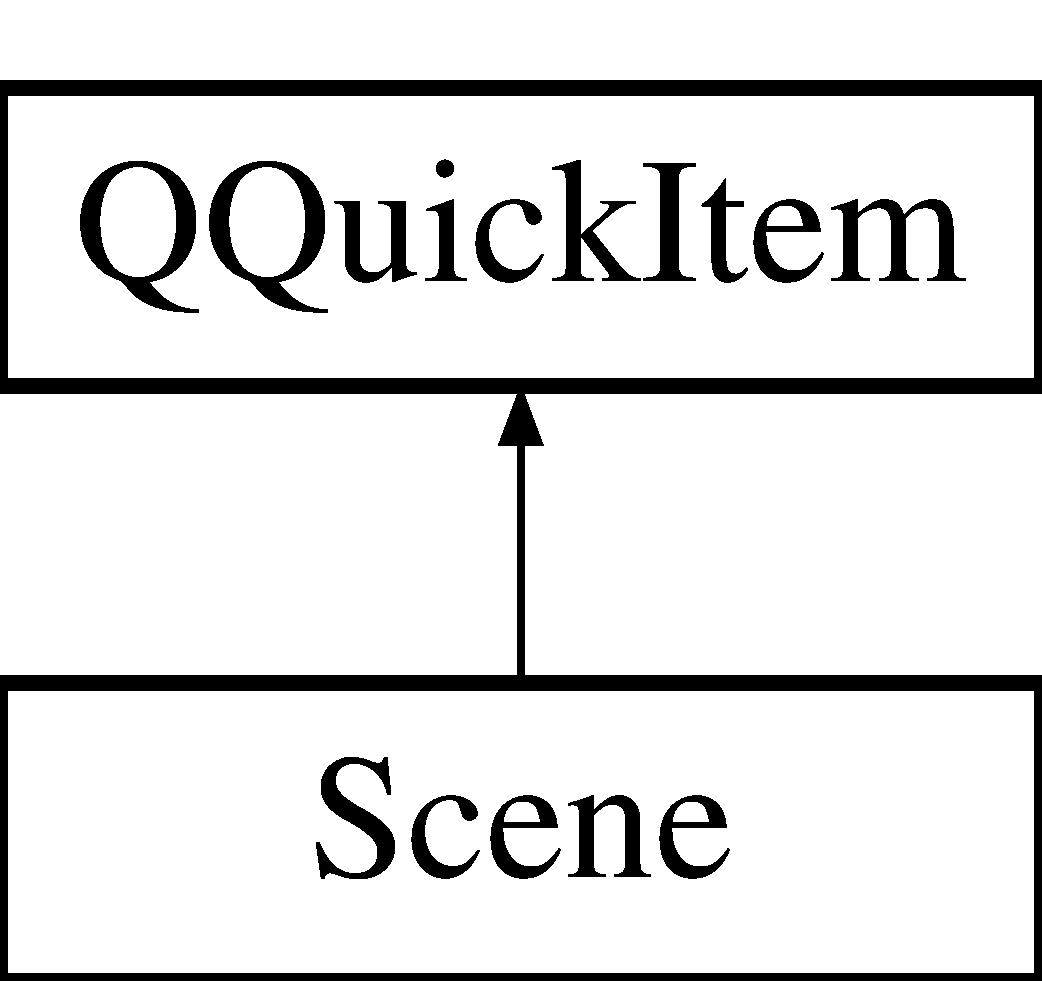
\includegraphics[height=2.000000cm]{class_scene}
\end{center}
\end{figure}
\subsection*{Public Slots}
\begin{DoxyCompactItemize}
\item 
virtual void \hyperlink{class_scene_a0c9213091fb06643b95801d2b406878f}{update} (int elapsed\+Time)
\item 
void \hyperlink{class_scene_a3f593e4e80703153633a76cc628ab539}{handle\+Game\+Lost} ()
\item 
void \hyperlink{class_scene_aceda1edb06b179bd439539965998f7da}{handle\+Game\+Started} ()
\item 
void \hyperlink{class_scene_ace3407a4d148d317a20b1bf205554bc5}{register\+Navigation} (\hyperlink{class_navigation}{Navigation} $\ast$navigation)
\item 
void \hyperlink{class_scene_ade6d7968a2bad7c1dfbae98045a8aa7d}{rotate\+Current\+Gem} (const Q\+Quaternion \&quaternion)
\end{DoxyCompactItemize}
\subsection*{Signals}
\begin{DoxyCompactItemize}
\item 
void \hyperlink{class_scene_a9c23e7cda34a3089165ce18c2ec89c15}{cubes\+Changed} ()
\item 
void \hyperlink{class_scene_a8df7e2ef0bf2910fa03df1c16b255551}{geometries\+Changed} ()
\item 
void \hyperlink{class_scene_a4eed91c96f13a7646830737b820755c4}{root\+Light\+Ray\+Changed} ()
\item 
void \hyperlink{class_scene_a700dd8faf803b34d7b374c5aded06d45}{game\+Started} ()
\item 
void \hyperlink{class_scene_aa73ff5f1f6c873357149afe83c749d09}{game\+Lost} ()
\end{DoxyCompactItemize}
\subsection*{Public Member Functions}
\begin{DoxyCompactItemize}
\item 
\hyperlink{class_scene_a93f88c89ce94ad70a668225522818b1e}{Scene} (Q\+Quick\+Item $\ast$parent=0)
\begin{DoxyCompactList}\small\item\em Creates a new scene without any further information.  Before use scene you have to set \hyperlink{class_scene_a65753673cd72f8b921cda3ac10c31e87}{geometries()}, \hyperlink{class_scene_a437a4ce938a6de368c2a6abba0ec3f3d}{root\+Light\+Ray()}, \hyperlink{class_scene_ab915c54546b8cecc3ae6bb7c8983518c}{camera()}, \hyperlink{class_scene_ae8f457e7e69cac64f533e02f4f13e725}{preview\+Camera()} and \hyperlink{class_scene_ace3407a4d148d317a20b1bf205554bc5}{register\+Navigation()} \end{DoxyCompactList}\item 
virtual \hyperlink{class_scene_a3b8cec2e32546713915f8c6303c951f1}{$\sim$\+Scene} ()
\item 
Q\+Qml\+List\+Property$<$ \hyperlink{class_abstract_gem}{Abstract\+Gem} $>$ \hyperlink{class_scene_ac437a983a495358875b319a4fcf912d4}{geometries\+Q\+M\+L} ()
\begin{DoxyCompactList}\small\item\em Allow Q\+M\+L classes to read our gems.  Initially it was planned to manipulate our gems from Q\+M\+L classes, but we did not get it to work. Now we create it over a J\+S\+O\+N-\/object and set it once, which works. All in all gem manipulation from Q\+M\+L is magic and we do not know why and how it really works. \end{DoxyCompactList}\item 
\hyperlink{class_q_list}{Q\+List}$<$ \hyperlink{class_abstract_gem}{Abstract\+Gem} $\ast$ $>$ \hyperlink{class_scene_a65753673cd72f8b921cda3ac10c31e87}{geometries} ()
\item 
\hyperlink{class_camera}{Camera} $\ast$ \hyperlink{class_scene_a81b014ae882dfaec147d917b1ea99d68}{camera} () const 
\item 
void \hyperlink{class_scene_a4c722c43b266a642a4a06d0d818b14d1}{set\+Camera} (\hyperlink{class_camera}{Camera} $\ast$\hyperlink{class_scene_ab915c54546b8cecc3ae6bb7c8983518c}{camera})
\item 
\hyperlink{class_camera}{Camera} $\ast$ \hyperlink{class_scene_acdd91b41ac71a9e44b6e9883a30a1c48}{preview\+Camera} () const 
\item 
void \hyperlink{class_scene_a84120dfbddf207c955e16b7aae975b8c}{set\+Preview\+Camera} (\hyperlink{class_camera}{Camera} $\ast$\hyperlink{class_scene_ab915c54546b8cecc3ae6bb7c8983518c}{camera})
\item 
\hyperlink{class_abstract_gem}{Abstract\+Gem} $\ast$ \hyperlink{class_scene_af96ea722705769055ef2f9e9572f3fa0}{find\+Gem\+With\+Bounding\+Sphere\+Intersected\+By} (const \hyperlink{class_light_ray}{Light\+Ray} \&ray, Q\+Vector3\+D $\ast$collision\+Point=nullptr) const 
\begin{DoxyCompactList}\small\item\em Finds the nearest gem, that bounding sphere is intersected by given ray. \end{DoxyCompactList}\item 
\hyperlink{class_abstract_gem}{Abstract\+Gem} $\ast$ \hyperlink{class_scene_a2a2cee0a97d8436aac1cd582904af459}{find\+Gem\+Intersected\+By} (const \hyperlink{class_light_ray}{Light\+Ray} \&ray, Q\+Vector3\+D $\ast$collision\+Point=nullptr) const 
\begin{DoxyCompactList}\small\item\em Finds the nearest gem with bounding sphere intersected by given ray. \end{DoxyCompactList}\item 
void \hyperlink{class_scene_afcaeead320358b9d9dd02a113ef97c44}{set\+Current\+Gem} (\hyperlink{class_abstract_gem}{Abstract\+Gem} $\ast$current\+Gem)
\begin{DoxyCompactList}\small\item\em Set the gem, that will be controlled by player. \end{DoxyCompactList}\item 
\hyperlink{class_light_ray}{Light\+Ray} $\ast$ \hyperlink{class_scene_a7de6dcc38dd6398f71af71295ae09966}{root\+Light\+Ray} () const 
\item 
void \hyperlink{class_scene_a3da6be3089fe335bf628ef58d23cda18}{set\+Root\+Light\+Ray} (\hyperlink{class_light_ray}{Light\+Ray} $\ast$\hyperlink{class_scene_a437a4ce938a6de368c2a6abba0ec3f3d}{root\+Light\+Ray})
\end{DoxyCompactItemize}
\subsection*{Protected Attributes}
\begin{DoxyCompactItemize}
\item 
\hyperlink{class_scene_bounds}{Scene\+Bounds} $\ast$ \hyperlink{class_scene_a62831eb6a67ce74ee608b4327bf069f3}{m\+\_\+bounds}
\item 
\hyperlink{class_camera}{Camera} $\ast$ \hyperlink{class_scene_ab37f5e133a5fe0803c3df42a4fcba7bf}{m\+\_\+camera}
\item 
\hyperlink{class_camera}{Camera} $\ast$ \hyperlink{class_scene_af1841b6c042a5edcf39653706f17cdd1}{m\+\_\+preview\+Camera}
\item 
\hyperlink{class_abstract_gem}{Abstract\+Gem} $\ast$ \hyperlink{class_scene_aff9d5a2212ba1b5813dc10177f0344cb}{m\+\_\+current\+Gem}
\item 
\hyperlink{class_q_list}{Q\+List}$<$ \hyperlink{class_abstract_gem}{Abstract\+Gem} $\ast$ $>$ \hyperlink{class_scene_a47d7b35730d7959a640339ed11d18866}{m\+\_\+gems}
\item 
\hyperlink{class_navigation}{Navigation} $\ast$ \hyperlink{class_scene_a595ab554271bd87c4c73f0cce175ff81}{m\+\_\+navigation}
\item 
\hyperlink{class_light_ray}{Light\+Ray} $\ast$ \hyperlink{class_scene_a766daf7b6a92c877f1fc57f3d8af9959}{m\+\_\+root\+Light\+Ray}
\end{DoxyCompactItemize}
\subsection*{Properties}
\begin{DoxyCompactItemize}
\item 
Q\+Qml\+List\+Property$<$ \hyperlink{class_abstract_gem}{Abstract\+Gem} $>$ \hyperlink{class_scene_a426e8a21801c9cc93c5cd90896ed745d}{geometries}
\item 
\hyperlink{class_camera}{Camera} \hyperlink{class_scene_ab915c54546b8cecc3ae6bb7c8983518c}{camera}
\item 
\hyperlink{class_camera}{Camera} \hyperlink{class_scene_ae8f457e7e69cac64f533e02f4f13e725}{preview\+Camera}
\item 
\hyperlink{class_light_ray}{Light\+Ray} \hyperlink{class_scene_a437a4ce938a6de368c2a6abba0ec3f3d}{root\+Light\+Ray}
\end{DoxyCompactItemize}


\subsection{Detailed Description}
The \hyperlink{class_scene}{Scene} class provides access to geometry and collision detection methods. Furthermore some game logic is implemented, so the scene holds the player, the gem inflicted by player and cameras. 

\subsection{Constructor \& Destructor Documentation}
\hypertarget{class_scene_a93f88c89ce94ad70a668225522818b1e}{}\index{Scene@{Scene}!Scene@{Scene}}
\index{Scene@{Scene}!Scene@{Scene}}
\subsubsection[{Scene}]{\setlength{\rightskip}{0pt plus 5cm}Scene\+::\+Scene (
\begin{DoxyParamCaption}
\item[{Q\+Quick\+Item $\ast$}]{parent = {\ttfamily 0}}
\end{DoxyParamCaption}
)\hspace{0.3cm}{\ttfamily [explicit]}}\label{class_scene_a93f88c89ce94ad70a668225522818b1e}


Creates a new scene without any further information.  Before use scene you have to set \hyperlink{class_scene_a65753673cd72f8b921cda3ac10c31e87}{geometries()}, \hyperlink{class_scene_a437a4ce938a6de368c2a6abba0ec3f3d}{root\+Light\+Ray()}, \hyperlink{class_scene_ab915c54546b8cecc3ae6bb7c8983518c}{camera()}, \hyperlink{class_scene_ae8f457e7e69cac64f533e02f4f13e725}{preview\+Camera()} and \hyperlink{class_scene_ace3407a4d148d317a20b1bf205554bc5}{register\+Navigation()} 


\begin{DoxyParams}{Parameters}
{\em parent} & \\
\hline
\end{DoxyParams}
\hypertarget{class_scene_a3b8cec2e32546713915f8c6303c951f1}{}\index{Scene@{Scene}!````~Scene@{$\sim$\+Scene}}
\index{````~Scene@{$\sim$\+Scene}!Scene@{Scene}}
\subsubsection[{$\sim$\+Scene}]{\setlength{\rightskip}{0pt plus 5cm}Scene\+::$\sim$\+Scene (
\begin{DoxyParamCaption}
{}
\end{DoxyParamCaption}
)\hspace{0.3cm}{\ttfamily [virtual]}}\label{class_scene_a3b8cec2e32546713915f8c6303c951f1}


\subsection{Member Function Documentation}
\hypertarget{class_scene_a81b014ae882dfaec147d917b1ea99d68}{}\index{Scene@{Scene}!camera@{camera}}
\index{camera@{camera}!Scene@{Scene}}
\subsubsection[{camera}]{\setlength{\rightskip}{0pt plus 5cm}{\bf Camera}$\ast$ Scene\+::camera (
\begin{DoxyParamCaption}
{}
\end{DoxyParamCaption}
) const}\label{class_scene_a81b014ae882dfaec147d917b1ea99d68}
\hypertarget{class_scene_a9c23e7cda34a3089165ce18c2ec89c15}{}\index{Scene@{Scene}!cubes\+Changed@{cubes\+Changed}}
\index{cubes\+Changed@{cubes\+Changed}!Scene@{Scene}}
\subsubsection[{cubes\+Changed}]{\setlength{\rightskip}{0pt plus 5cm}void Scene\+::cubes\+Changed (
\begin{DoxyParamCaption}
{}
\end{DoxyParamCaption}
)\hspace{0.3cm}{\ttfamily [signal]}}\label{class_scene_a9c23e7cda34a3089165ce18c2ec89c15}
\hypertarget{class_scene_a2a2cee0a97d8436aac1cd582904af459}{}\index{Scene@{Scene}!find\+Gem\+Intersected\+By@{find\+Gem\+Intersected\+By}}
\index{find\+Gem\+Intersected\+By@{find\+Gem\+Intersected\+By}!Scene@{Scene}}
\subsubsection[{find\+Gem\+Intersected\+By}]{\setlength{\rightskip}{0pt plus 5cm}{\bf Abstract\+Gem} $\ast$ Scene\+::find\+Gem\+Intersected\+By (
\begin{DoxyParamCaption}
\item[{const {\bf Light\+Ray} \&}]{ray, }
\item[{Q\+Vector3\+D $\ast$}]{collision\+Point = {\ttfamily nullptr}}
\end{DoxyParamCaption}
) const}\label{class_scene_a2a2cee0a97d8436aac1cd582904af459}


Finds the nearest gem with bounding sphere intersected by given ray. 


\begin{DoxyParams}{Parameters}
{\em ray} & Ray send into scene to find gem. \\
\hline
{\em collision\+Point} & Optional parameter. The point of collision is written into. \\
\hline
\end{DoxyParams}
\begin{DoxyReturn}{Returns}
Returns the nearst intersected gem. Returns never a nullptr; 
\end{DoxyReturn}
\hypertarget{class_scene_af96ea722705769055ef2f9e9572f3fa0}{}\index{Scene@{Scene}!find\+Gem\+With\+Bounding\+Sphere\+Intersected\+By@{find\+Gem\+With\+Bounding\+Sphere\+Intersected\+By}}
\index{find\+Gem\+With\+Bounding\+Sphere\+Intersected\+By@{find\+Gem\+With\+Bounding\+Sphere\+Intersected\+By}!Scene@{Scene}}
\subsubsection[{find\+Gem\+With\+Bounding\+Sphere\+Intersected\+By}]{\setlength{\rightskip}{0pt plus 5cm}{\bf Abstract\+Gem} $\ast$ Scene\+::find\+Gem\+With\+Bounding\+Sphere\+Intersected\+By (
\begin{DoxyParamCaption}
\item[{const {\bf Light\+Ray} \&}]{ray, }
\item[{Q\+Vector3\+D $\ast$}]{collision\+Point = {\ttfamily nullptr}}
\end{DoxyParamCaption}
) const}\label{class_scene_af96ea722705769055ef2f9e9572f3fa0}


Finds the nearest gem, that bounding sphere is intersected by given ray. 


\begin{DoxyParams}{Parameters}
{\em ray} & Ray send into scene to find gem. \\
\hline
{\em collision\+Point} & Optional parameter. The point of collision is written into. Only if no nullptr is returned this value is useable. \\
\hline
\end{DoxyParams}
\begin{DoxyReturn}{Returns}
Returns the nearst intersected gem. Returns never nullptr. 
\end{DoxyReturn}
\hypertarget{class_scene_aa73ff5f1f6c873357149afe83c749d09}{}\index{Scene@{Scene}!game\+Lost@{game\+Lost}}
\index{game\+Lost@{game\+Lost}!Scene@{Scene}}
\subsubsection[{game\+Lost}]{\setlength{\rightskip}{0pt plus 5cm}void Scene\+::game\+Lost (
\begin{DoxyParamCaption}
{}
\end{DoxyParamCaption}
)\hspace{0.3cm}{\ttfamily [signal]}}\label{class_scene_aa73ff5f1f6c873357149afe83c749d09}
\hypertarget{class_scene_a700dd8faf803b34d7b374c5aded06d45}{}\index{Scene@{Scene}!game\+Started@{game\+Started}}
\index{game\+Started@{game\+Started}!Scene@{Scene}}
\subsubsection[{game\+Started}]{\setlength{\rightskip}{0pt plus 5cm}void Scene\+::game\+Started (
\begin{DoxyParamCaption}
{}
\end{DoxyParamCaption}
)\hspace{0.3cm}{\ttfamily [signal]}}\label{class_scene_a700dd8faf803b34d7b374c5aded06d45}
\hypertarget{class_scene_a65753673cd72f8b921cda3ac10c31e87}{}\index{Scene@{Scene}!geometries@{geometries}}
\index{geometries@{geometries}!Scene@{Scene}}
\subsubsection[{geometries}]{\setlength{\rightskip}{0pt plus 5cm}{\bf Q\+List}$<${\bf Abstract\+Gem} $\ast$$>$ Scene\+::geometries (
\begin{DoxyParamCaption}
{}
\end{DoxyParamCaption}
)}\label{class_scene_a65753673cd72f8b921cda3ac10c31e87}
\hypertarget{class_scene_a8df7e2ef0bf2910fa03df1c16b255551}{}\index{Scene@{Scene}!geometries\+Changed@{geometries\+Changed}}
\index{geometries\+Changed@{geometries\+Changed}!Scene@{Scene}}
\subsubsection[{geometries\+Changed}]{\setlength{\rightskip}{0pt plus 5cm}void Scene\+::geometries\+Changed (
\begin{DoxyParamCaption}
{}
\end{DoxyParamCaption}
)\hspace{0.3cm}{\ttfamily [signal]}}\label{class_scene_a8df7e2ef0bf2910fa03df1c16b255551}
\hypertarget{class_scene_ac437a983a495358875b319a4fcf912d4}{}\index{Scene@{Scene}!geometries\+Q\+M\+L@{geometries\+Q\+M\+L}}
\index{geometries\+Q\+M\+L@{geometries\+Q\+M\+L}!Scene@{Scene}}
\subsubsection[{geometries\+Q\+M\+L}]{\setlength{\rightskip}{0pt plus 5cm}Q\+Qml\+List\+Property$<$ {\bf Abstract\+Gem} $>$ Scene\+::geometries\+Q\+M\+L (
\begin{DoxyParamCaption}
{}
\end{DoxyParamCaption}
)}\label{class_scene_ac437a983a495358875b319a4fcf912d4}


Allow Q\+M\+L classes to read our gems.  Initially it was planned to manipulate our gems from Q\+M\+L classes, but we did not get it to work. Now we create it over a J\+S\+O\+N-\/object and set it once, which works. All in all gem manipulation from Q\+M\+L is magic and we do not know why and how it really works. 

\begin{DoxyReturn}{Returns}
Returns a List of Gems which is supported by Q\+M\+L. 
\end{DoxyReturn}
\hypertarget{class_scene_a3f593e4e80703153633a76cc628ab539}{}\index{Scene@{Scene}!handle\+Game\+Lost@{handle\+Game\+Lost}}
\index{handle\+Game\+Lost@{handle\+Game\+Lost}!Scene@{Scene}}
\subsubsection[{handle\+Game\+Lost}]{\setlength{\rightskip}{0pt plus 5cm}void Scene\+::handle\+Game\+Lost (
\begin{DoxyParamCaption}
{}
\end{DoxyParamCaption}
)\hspace{0.3cm}{\ttfamily [slot]}}\label{class_scene_a3f593e4e80703153633a76cc628ab539}
\hypertarget{class_scene_aceda1edb06b179bd439539965998f7da}{}\index{Scene@{Scene}!handle\+Game\+Started@{handle\+Game\+Started}}
\index{handle\+Game\+Started@{handle\+Game\+Started}!Scene@{Scene}}
\subsubsection[{handle\+Game\+Started}]{\setlength{\rightskip}{0pt plus 5cm}void Scene\+::handle\+Game\+Started (
\begin{DoxyParamCaption}
{}
\end{DoxyParamCaption}
)\hspace{0.3cm}{\ttfamily [slot]}}\label{class_scene_aceda1edb06b179bd439539965998f7da}
\hypertarget{class_scene_acdd91b41ac71a9e44b6e9883a30a1c48}{}\index{Scene@{Scene}!preview\+Camera@{preview\+Camera}}
\index{preview\+Camera@{preview\+Camera}!Scene@{Scene}}
\subsubsection[{preview\+Camera}]{\setlength{\rightskip}{0pt plus 5cm}{\bf Camera}$\ast$ Scene\+::preview\+Camera (
\begin{DoxyParamCaption}
{}
\end{DoxyParamCaption}
) const}\label{class_scene_acdd91b41ac71a9e44b6e9883a30a1c48}
\hypertarget{class_scene_ace3407a4d148d317a20b1bf205554bc5}{}\index{Scene@{Scene}!register\+Navigation@{register\+Navigation}}
\index{register\+Navigation@{register\+Navigation}!Scene@{Scene}}
\subsubsection[{register\+Navigation}]{\setlength{\rightskip}{0pt plus 5cm}void Scene\+::register\+Navigation (
\begin{DoxyParamCaption}
\item[{{\bf Navigation} $\ast$}]{navigation}
\end{DoxyParamCaption}
)\hspace{0.3cm}{\ttfamily [slot]}}\label{class_scene_ace3407a4d148d317a20b1bf205554bc5}
\hypertarget{class_scene_a7de6dcc38dd6398f71af71295ae09966}{}\index{Scene@{Scene}!root\+Light\+Ray@{root\+Light\+Ray}}
\index{root\+Light\+Ray@{root\+Light\+Ray}!Scene@{Scene}}
\subsubsection[{root\+Light\+Ray}]{\setlength{\rightskip}{0pt plus 5cm}{\bf Light\+Ray}$\ast$ Scene\+::root\+Light\+Ray (
\begin{DoxyParamCaption}
{}
\end{DoxyParamCaption}
) const}\label{class_scene_a7de6dcc38dd6398f71af71295ae09966}
\hypertarget{class_scene_a4eed91c96f13a7646830737b820755c4}{}\index{Scene@{Scene}!root\+Light\+Ray\+Changed@{root\+Light\+Ray\+Changed}}
\index{root\+Light\+Ray\+Changed@{root\+Light\+Ray\+Changed}!Scene@{Scene}}
\subsubsection[{root\+Light\+Ray\+Changed}]{\setlength{\rightskip}{0pt plus 5cm}void Scene\+::root\+Light\+Ray\+Changed (
\begin{DoxyParamCaption}
{}
\end{DoxyParamCaption}
)\hspace{0.3cm}{\ttfamily [signal]}}\label{class_scene_a4eed91c96f13a7646830737b820755c4}
\hypertarget{class_scene_ade6d7968a2bad7c1dfbae98045a8aa7d}{}\index{Scene@{Scene}!rotate\+Current\+Gem@{rotate\+Current\+Gem}}
\index{rotate\+Current\+Gem@{rotate\+Current\+Gem}!Scene@{Scene}}
\subsubsection[{rotate\+Current\+Gem}]{\setlength{\rightskip}{0pt plus 5cm}void Scene\+::rotate\+Current\+Gem (
\begin{DoxyParamCaption}
\item[{const Q\+Quaternion \&}]{quaternion}
\end{DoxyParamCaption}
)\hspace{0.3cm}{\ttfamily [slot]}}\label{class_scene_ade6d7968a2bad7c1dfbae98045a8aa7d}
\hypertarget{class_scene_a4c722c43b266a642a4a06d0d818b14d1}{}\index{Scene@{Scene}!set\+Camera@{set\+Camera}}
\index{set\+Camera@{set\+Camera}!Scene@{Scene}}
\subsubsection[{set\+Camera}]{\setlength{\rightskip}{0pt plus 5cm}void Scene\+::set\+Camera (
\begin{DoxyParamCaption}
\item[{{\bf Camera} $\ast$}]{camera}
\end{DoxyParamCaption}
)}\label{class_scene_a4c722c43b266a642a4a06d0d818b14d1}
\hypertarget{class_scene_afcaeead320358b9d9dd02a113ef97c44}{}\index{Scene@{Scene}!set\+Current\+Gem@{set\+Current\+Gem}}
\index{set\+Current\+Gem@{set\+Current\+Gem}!Scene@{Scene}}
\subsubsection[{set\+Current\+Gem}]{\setlength{\rightskip}{0pt plus 5cm}void Scene\+::set\+Current\+Gem (
\begin{DoxyParamCaption}
\item[{{\bf Abstract\+Gem} $\ast$}]{current\+Gem}
\end{DoxyParamCaption}
)}\label{class_scene_afcaeead320358b9d9dd02a113ef97c44}


Set the gem, that will be controlled by player. 


\begin{DoxyParams}{Parameters}
{\em current\+Gem} & The gem that will be controlled by player. \\
\hline
\end{DoxyParams}
\hypertarget{class_scene_a84120dfbddf207c955e16b7aae975b8c}{}\index{Scene@{Scene}!set\+Preview\+Camera@{set\+Preview\+Camera}}
\index{set\+Preview\+Camera@{set\+Preview\+Camera}!Scene@{Scene}}
\subsubsection[{set\+Preview\+Camera}]{\setlength{\rightskip}{0pt plus 5cm}void Scene\+::set\+Preview\+Camera (
\begin{DoxyParamCaption}
\item[{{\bf Camera} $\ast$}]{camera}
\end{DoxyParamCaption}
)}\label{class_scene_a84120dfbddf207c955e16b7aae975b8c}
\hypertarget{class_scene_a3da6be3089fe335bf628ef58d23cda18}{}\index{Scene@{Scene}!set\+Root\+Light\+Ray@{set\+Root\+Light\+Ray}}
\index{set\+Root\+Light\+Ray@{set\+Root\+Light\+Ray}!Scene@{Scene}}
\subsubsection[{set\+Root\+Light\+Ray}]{\setlength{\rightskip}{0pt plus 5cm}void Scene\+::set\+Root\+Light\+Ray (
\begin{DoxyParamCaption}
\item[{{\bf Light\+Ray} $\ast$}]{root\+Light\+Ray}
\end{DoxyParamCaption}
)}\label{class_scene_a3da6be3089fe335bf628ef58d23cda18}
\hypertarget{class_scene_a0c9213091fb06643b95801d2b406878f}{}\index{Scene@{Scene}!update@{update}}
\index{update@{update}!Scene@{Scene}}
\subsubsection[{update}]{\setlength{\rightskip}{0pt plus 5cm}void Scene\+::update (
\begin{DoxyParamCaption}
\item[{int}]{elapsed\+Time}
\end{DoxyParamCaption}
)\hspace{0.3cm}{\ttfamily [virtual]}, {\ttfamily [slot]}}\label{class_scene_a0c9213091fb06643b95801d2b406878f}


\subsection{Member Data Documentation}
\hypertarget{class_scene_a62831eb6a67ce74ee608b4327bf069f3}{}\index{Scene@{Scene}!m\+\_\+bounds@{m\+\_\+bounds}}
\index{m\+\_\+bounds@{m\+\_\+bounds}!Scene@{Scene}}
\subsubsection[{m\+\_\+bounds}]{\setlength{\rightskip}{0pt plus 5cm}{\bf Scene\+Bounds}$\ast$ Scene\+::m\+\_\+bounds\hspace{0.3cm}{\ttfamily [protected]}}\label{class_scene_a62831eb6a67ce74ee608b4327bf069f3}
\hypertarget{class_scene_ab37f5e133a5fe0803c3df42a4fcba7bf}{}\index{Scene@{Scene}!m\+\_\+camera@{m\+\_\+camera}}
\index{m\+\_\+camera@{m\+\_\+camera}!Scene@{Scene}}
\subsubsection[{m\+\_\+camera}]{\setlength{\rightskip}{0pt plus 5cm}{\bf Camera}$\ast$ Scene\+::m\+\_\+camera\hspace{0.3cm}{\ttfamily [protected]}}\label{class_scene_ab37f5e133a5fe0803c3df42a4fcba7bf}
\hypertarget{class_scene_aff9d5a2212ba1b5813dc10177f0344cb}{}\index{Scene@{Scene}!m\+\_\+current\+Gem@{m\+\_\+current\+Gem}}
\index{m\+\_\+current\+Gem@{m\+\_\+current\+Gem}!Scene@{Scene}}
\subsubsection[{m\+\_\+current\+Gem}]{\setlength{\rightskip}{0pt plus 5cm}{\bf Abstract\+Gem}$\ast$ Scene\+::m\+\_\+current\+Gem\hspace{0.3cm}{\ttfamily [protected]}}\label{class_scene_aff9d5a2212ba1b5813dc10177f0344cb}
\hypertarget{class_scene_a47d7b35730d7959a640339ed11d18866}{}\index{Scene@{Scene}!m\+\_\+gems@{m\+\_\+gems}}
\index{m\+\_\+gems@{m\+\_\+gems}!Scene@{Scene}}
\subsubsection[{m\+\_\+gems}]{\setlength{\rightskip}{0pt plus 5cm}{\bf Q\+List}$<${\bf Abstract\+Gem}$\ast$$>$ Scene\+::m\+\_\+gems\hspace{0.3cm}{\ttfamily [protected]}}\label{class_scene_a47d7b35730d7959a640339ed11d18866}
\hypertarget{class_scene_a595ab554271bd87c4c73f0cce175ff81}{}\index{Scene@{Scene}!m\+\_\+navigation@{m\+\_\+navigation}}
\index{m\+\_\+navigation@{m\+\_\+navigation}!Scene@{Scene}}
\subsubsection[{m\+\_\+navigation}]{\setlength{\rightskip}{0pt plus 5cm}{\bf Navigation}$\ast$ Scene\+::m\+\_\+navigation\hspace{0.3cm}{\ttfamily [protected]}}\label{class_scene_a595ab554271bd87c4c73f0cce175ff81}
\hypertarget{class_scene_af1841b6c042a5edcf39653706f17cdd1}{}\index{Scene@{Scene}!m\+\_\+preview\+Camera@{m\+\_\+preview\+Camera}}
\index{m\+\_\+preview\+Camera@{m\+\_\+preview\+Camera}!Scene@{Scene}}
\subsubsection[{m\+\_\+preview\+Camera}]{\setlength{\rightskip}{0pt plus 5cm}{\bf Camera}$\ast$ Scene\+::m\+\_\+preview\+Camera\hspace{0.3cm}{\ttfamily [protected]}}\label{class_scene_af1841b6c042a5edcf39653706f17cdd1}
\hypertarget{class_scene_a766daf7b6a92c877f1fc57f3d8af9959}{}\index{Scene@{Scene}!m\+\_\+root\+Light\+Ray@{m\+\_\+root\+Light\+Ray}}
\index{m\+\_\+root\+Light\+Ray@{m\+\_\+root\+Light\+Ray}!Scene@{Scene}}
\subsubsection[{m\+\_\+root\+Light\+Ray}]{\setlength{\rightskip}{0pt plus 5cm}{\bf Light\+Ray}$\ast$ Scene\+::m\+\_\+root\+Light\+Ray\hspace{0.3cm}{\ttfamily [protected]}}\label{class_scene_a766daf7b6a92c877f1fc57f3d8af9959}


\subsection{Property Documentation}
\hypertarget{class_scene_ab915c54546b8cecc3ae6bb7c8983518c}{}\index{Scene@{Scene}!camera@{camera}}
\index{camera@{camera}!Scene@{Scene}}
\subsubsection[{camera}]{\setlength{\rightskip}{0pt plus 5cm}{\bf Camera} $\ast$ Scene\+::camera\hspace{0.3cm}{\ttfamily [read]}, {\ttfamily [write]}}\label{class_scene_ab915c54546b8cecc3ae6bb7c8983518c}
\hypertarget{class_scene_a426e8a21801c9cc93c5cd90896ed745d}{}\index{Scene@{Scene}!geometries@{geometries}}
\index{geometries@{geometries}!Scene@{Scene}}
\subsubsection[{geometries}]{\setlength{\rightskip}{0pt plus 5cm}{\bf Q\+List}$<$ {\bf Abstract\+Gem} $\ast$ $>$ Scene\+::geometries\hspace{0.3cm}{\ttfamily [read]}}\label{class_scene_a426e8a21801c9cc93c5cd90896ed745d}
\hypertarget{class_scene_ae8f457e7e69cac64f533e02f4f13e725}{}\index{Scene@{Scene}!preview\+Camera@{preview\+Camera}}
\index{preview\+Camera@{preview\+Camera}!Scene@{Scene}}
\subsubsection[{preview\+Camera}]{\setlength{\rightskip}{0pt plus 5cm}{\bf Camera} $\ast$ Scene\+::preview\+Camera\hspace{0.3cm}{\ttfamily [read]}, {\ttfamily [write]}}\label{class_scene_ae8f457e7e69cac64f533e02f4f13e725}
\hypertarget{class_scene_a437a4ce938a6de368c2a6abba0ec3f3d}{}\index{Scene@{Scene}!root\+Light\+Ray@{root\+Light\+Ray}}
\index{root\+Light\+Ray@{root\+Light\+Ray}!Scene@{Scene}}
\subsubsection[{root\+Light\+Ray}]{\setlength{\rightskip}{0pt plus 5cm}{\bf Light\+Ray} $\ast$ Scene\+::root\+Light\+Ray\hspace{0.3cm}{\ttfamily [read]}, {\ttfamily [write]}}\label{class_scene_a437a4ce938a6de368c2a6abba0ec3f3d}


The documentation for this class was generated from the following files\+:\begin{DoxyCompactItemize}
\item 
Game-\/\+Programming-\/\+W\+S2014/gem\+Illuminator/\hyperlink{scene_8h}{scene.\+h}\item 
Game-\/\+Programming-\/\+W\+S2014/gem\+Illuminator/\hyperlink{scene_8cpp}{scene.\+cpp}\end{DoxyCompactItemize}

\hypertarget{class_scene_bounds}{\section{Scene\+Bounds Class Reference}
\label{class_scene_bounds}\index{Scene\+Bounds@{Scene\+Bounds}}
}


The \hyperlink{class_scene_bounds}{Scene\+Bounds} class is a special kind of gem describing the bounds of scene. The shape of the bounds is a cube, with a given extent in each direction.  The main reason that the bounds are also a gem is easier collision detection. If we have bounds around our scene every ray emitted into scene will hit something. Furthermore the collision with scene bounds can be processed in a way, that the player will lose if the player hits the bounds.  




{\ttfamily \#include $<$scenebounds.\+h$>$}

Inheritance diagram for Scene\+Bounds\+:\begin{figure}[H]
\begin{center}
\leavevmode
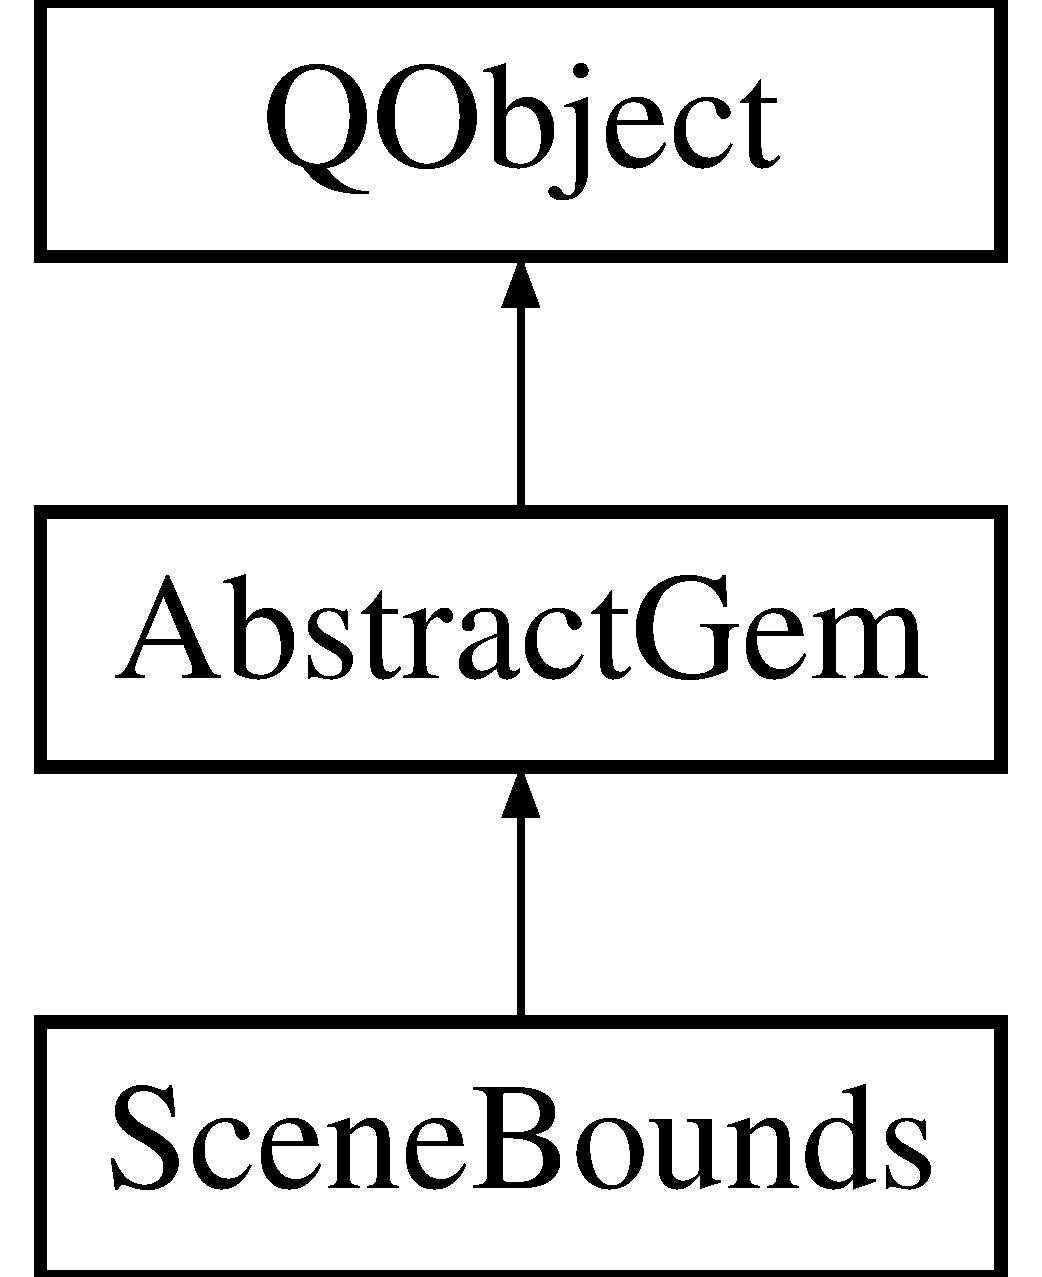
\includegraphics[height=3.000000cm]{class_scene_bounds}
\end{center}
\end{figure}
\subsection*{Public Member Functions}
\begin{DoxyCompactItemize}
\item 
\hyperlink{class_scene_bounds_a26e24012c6a45d3412745828b037dae4}{Scene\+Bounds} (Q\+Object $\ast$parent=0)
\begin{DoxyCompactList}\small\item\em Creates new \hyperlink{class_scene_bounds}{Scene\+Bounds}. The extent of bounds is taken from config file. \end{DoxyCompactList}\item 
virtual \hyperlink{class_scene_bounds_a625ef0d42c9133022a636ba5a57ad840}{$\sim$\+Scene\+Bounds} ()
\item 
void \hyperlink{class_scene_bounds_a26db5e7928d3ac7d0257dc52e1ed4e77}{set\+Position} (const Q\+Vector3\+D \&position) override
\begin{DoxyCompactList}\small\item\em Override \hyperlink{class_abstract_gem_aaf11fa4b522dc334ebed4f2d031a3e2b}{Abstract\+Gem\+::set\+Position()} in order to forbid moving the bounds around. \end{DoxyCompactList}\item 
void \hyperlink{class_scene_bounds_a2e7b2f2e66700b414584ca6b407faf72}{set\+Rotation} (const Q\+Quaternion \&rotation) override
\begin{DoxyCompactList}\small\item\em set\+Rotation Override \hyperlink{class_abstract_gem_afce4d09f74fec117d27b11a220eee6b9}{Abstract\+Gem\+::set\+Rotation()} in order to forbid rotating the bounds. \end{DoxyCompactList}\item 
\hyperlink{singleton_q_list}{Q\+List}$<$ \hyperlink{class_light_ray}{Light\+Ray} $\ast$ $>$ \hyperlink{class_scene_bounds_aeac6aafe6081e8efd6b4180e86346dc0}{process\+Ray\+Intersection} (const \hyperlink{class_light_ray}{Light\+Ray} \&ray, \hyperlink{class_scene}{Scene} $\ast$scene) override
\begin{DoxyCompactList}\small\item\em Override \hyperlink{class_abstract_gem_ab4f3c6d38acbe59a610c67588e4944d7}{Abstract\+Gem\+::process\+Ray\+Intersection()} in order to ensure the player loses hitting the bounds. \end{DoxyCompactList}\end{DoxyCompactItemize}
\subsection*{Additional Inherited Members}


\subsection{Detailed Description}
The \hyperlink{class_scene_bounds}{Scene\+Bounds} class is a special kind of gem describing the bounds of scene. The shape of the bounds is a cube, with a given extent in each direction.  The main reason that the bounds are also a gem is easier collision detection. If we have bounds around our scene every ray emitted into scene will hit something. Furthermore the collision with scene bounds can be processed in a way, that the player will lose if the player hits the bounds. 

\subsection{Constructor \& Destructor Documentation}
\hypertarget{class_scene_bounds_a26e24012c6a45d3412745828b037dae4}{\index{Scene\+Bounds@{Scene\+Bounds}!Scene\+Bounds@{Scene\+Bounds}}
\index{Scene\+Bounds@{Scene\+Bounds}!Scene\+Bounds@{Scene\+Bounds}}
\subsubsection[{Scene\+Bounds}]{\setlength{\rightskip}{0pt plus 5cm}Scene\+Bounds\+::\+Scene\+Bounds (
\begin{DoxyParamCaption}
\item[{Q\+Object $\ast$}]{parent = {\ttfamily 0}}
\end{DoxyParamCaption}
)\hspace{0.3cm}{\ttfamily [explicit]}}}\label{class_scene_bounds_a26e24012c6a45d3412745828b037dae4}


Creates new \hyperlink{class_scene_bounds}{Scene\+Bounds}. The extent of bounds is taken from config file. 


\begin{DoxyParams}{Parameters}
{\em parent} & \\
\hline
\end{DoxyParams}
\hypertarget{class_scene_bounds_a625ef0d42c9133022a636ba5a57ad840}{\index{Scene\+Bounds@{Scene\+Bounds}!````~Scene\+Bounds@{$\sim$\+Scene\+Bounds}}
\index{````~Scene\+Bounds@{$\sim$\+Scene\+Bounds}!Scene\+Bounds@{Scene\+Bounds}}
\subsubsection[{$\sim$\+Scene\+Bounds}]{\setlength{\rightskip}{0pt plus 5cm}Scene\+Bounds\+::$\sim$\+Scene\+Bounds (
\begin{DoxyParamCaption}
{}
\end{DoxyParamCaption}
)\hspace{0.3cm}{\ttfamily [virtual]}}}\label{class_scene_bounds_a625ef0d42c9133022a636ba5a57ad840}


\subsection{Member Function Documentation}
\hypertarget{class_scene_bounds_aeac6aafe6081e8efd6b4180e86346dc0}{\index{Scene\+Bounds@{Scene\+Bounds}!process\+Ray\+Intersection@{process\+Ray\+Intersection}}
\index{process\+Ray\+Intersection@{process\+Ray\+Intersection}!Scene\+Bounds@{Scene\+Bounds}}
\subsubsection[{process\+Ray\+Intersection}]{\setlength{\rightskip}{0pt plus 5cm}{\bf Q\+List}$<$ {\bf Light\+Ray} $\ast$ $>$ Scene\+Bounds\+::process\+Ray\+Intersection (
\begin{DoxyParamCaption}
\item[{const {\bf Light\+Ray} \&}]{ray, }
\item[{{\bf Scene} $\ast$}]{scene}
\end{DoxyParamCaption}
)\hspace{0.3cm}{\ttfamily [override]}, {\ttfamily [virtual]}}}\label{class_scene_bounds_aeac6aafe6081e8efd6b4180e86346dc0}


Override \hyperlink{class_abstract_gem_ab4f3c6d38acbe59a610c67588e4944d7}{Abstract\+Gem\+::process\+Ray\+Intersection()} in order to ensure the player loses hitting the bounds. 


\begin{DoxyParams}{Parameters}
{\em ray} & The ray hitting the bounds. \\
\hline
{\em scene} & The scene containing all lightrays. \\
\hline
\end{DoxyParams}
\begin{DoxyReturn}{Returns}
Returns a \hyperlink{singleton_q_list}{Q\+List} containing only a \hyperlink{class_game_lost_ray}{Game\+Lost\+Ray}, so the player will loose as soon as the player tries to move on returned ray. 
\end{DoxyReturn}


Reimplemented from \hyperlink{class_abstract_gem_ab4f3c6d38acbe59a610c67588e4944d7}{Abstract\+Gem}.

\hypertarget{class_scene_bounds_a26db5e7928d3ac7d0257dc52e1ed4e77}{\index{Scene\+Bounds@{Scene\+Bounds}!set\+Position@{set\+Position}}
\index{set\+Position@{set\+Position}!Scene\+Bounds@{Scene\+Bounds}}
\subsubsection[{set\+Position}]{\setlength{\rightskip}{0pt plus 5cm}void Scene\+Bounds\+::set\+Position (
\begin{DoxyParamCaption}
\item[{const Q\+Vector3\+D \&}]{position}
\end{DoxyParamCaption}
)\hspace{0.3cm}{\ttfamily [override]}, {\ttfamily [virtual]}}}\label{class_scene_bounds_a26db5e7928d3ac7d0257dc52e1ed4e77}


Override \hyperlink{class_abstract_gem_aaf11fa4b522dc334ebed4f2d031a3e2b}{Abstract\+Gem\+::set\+Position()} in order to forbid moving the bounds around. 


\begin{DoxyParams}{Parameters}
{\em position} & This parameter will be ignored. \\
\hline
\end{DoxyParams}


Reimplemented from \hyperlink{class_abstract_gem_aaf11fa4b522dc334ebed4f2d031a3e2b}{Abstract\+Gem}.

\hypertarget{class_scene_bounds_a2e7b2f2e66700b414584ca6b407faf72}{\index{Scene\+Bounds@{Scene\+Bounds}!set\+Rotation@{set\+Rotation}}
\index{set\+Rotation@{set\+Rotation}!Scene\+Bounds@{Scene\+Bounds}}
\subsubsection[{set\+Rotation}]{\setlength{\rightskip}{0pt plus 5cm}void Scene\+Bounds\+::set\+Rotation (
\begin{DoxyParamCaption}
\item[{const Q\+Quaternion \&}]{rotation}
\end{DoxyParamCaption}
)\hspace{0.3cm}{\ttfamily [override]}, {\ttfamily [virtual]}}}\label{class_scene_bounds_a2e7b2f2e66700b414584ca6b407faf72}


set\+Rotation Override \hyperlink{class_abstract_gem_afce4d09f74fec117d27b11a220eee6b9}{Abstract\+Gem\+::set\+Rotation()} in order to forbid rotating the bounds. 


\begin{DoxyParams}{Parameters}
{\em rotation} & This parameter will be ignored. \\
\hline
\end{DoxyParams}


Reimplemented from \hyperlink{class_abstract_gem_afce4d09f74fec117d27b11a220eee6b9}{Abstract\+Gem}.



The documentation for this class was generated from the following files\+:\begin{DoxyCompactItemize}
\item 
\hyperlink{scenebounds_8h}{scenebounds.\+h}\item 
\hyperlink{scenebounds_8cpp}{scenebounds.\+cpp}\end{DoxyCompactItemize}

\hypertarget{class_scene_renderer}{}\section{Scene\+Renderer Class Reference}
\label{class_scene_renderer}\index{Scene\+Renderer@{Scene\+Renderer}}


The \hyperlink{class_scene_renderer}{Scene\+Renderer} class  Renders the scene\+: Packs the scene in the buffer and draws the scene in as few render calls as possible. The \hyperlink{class_scene_renderer}{Scene\+Renderer} uses specialized Renderer for diffrent types of geometry.  




{\ttfamily \#include $<$scenerenderer.\+h$>$}

Inheritance diagram for Scene\+Renderer\+:\begin{figure}[H]
\begin{center}
\leavevmode
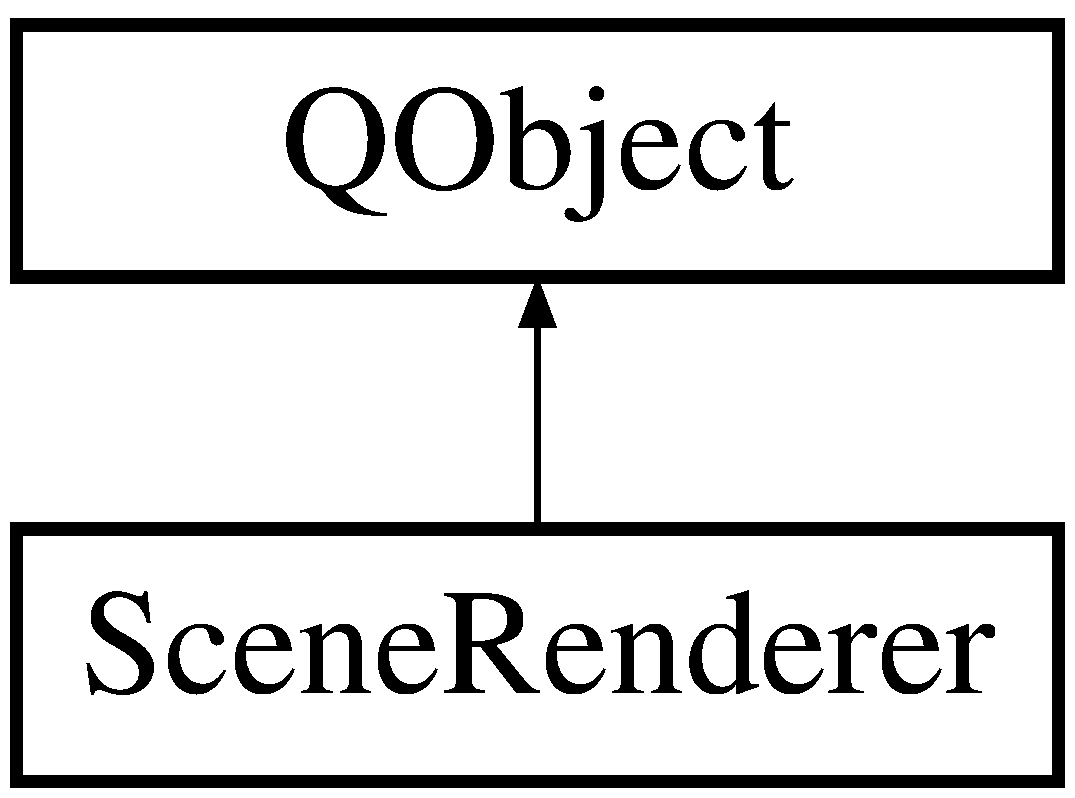
\includegraphics[height=2.000000cm]{class_scene_renderer}
\end{center}
\end{figure}
\subsection*{Public Slots}
\begin{DoxyCompactItemize}
\item 
void \hyperlink{class_scene_renderer_a91177b285ac9fba685e8409671eac1e7}{paint} (Q\+Open\+G\+L\+Functions \&gl, const Q\+Matrix4x4 \&view\+Projection, const \hyperlink{class_q_hash}{Q\+Hash}$<$ \hyperlink{shaderprograms_8h_ada89718f8d394b2cc093eb9770c554ff}{Shader\+Programs}, Q\+Open\+G\+L\+Shader\+Program $\ast$ $>$ \&shader\+Programs)
\begin{DoxyCompactList}\small\item\em paint Paints the previous synchronized scene using specified programs. \end{DoxyCompactList}\end{DoxyCompactItemize}
\subsection*{Signals}
\begin{DoxyCompactItemize}
\item 
void \hyperlink{class_scene_renderer_a9ea8f56371c7758519c5e6541519d988}{initalization\+Done} ()
\begin{DoxyCompactList}\small\item\em This signal is emitted after initialization of all ressources is done. \end{DoxyCompactList}\end{DoxyCompactItemize}
\subsection*{Public Member Functions}
\begin{DoxyCompactItemize}
\item 
\hyperlink{class_scene_renderer_a12f72dc9b22e99ecdccaec38b6d2d512}{Scene\+Renderer} (Q\+Object $\ast$parent=0)
\begin{DoxyCompactList}\small\item\em \hyperlink{class_scene_renderer}{Scene\+Renderer}. \end{DoxyCompactList}\item 
virtual \hyperlink{class_scene_renderer_aceec75b5c04861c2a5c26349c2ba5748}{$\sim$\+Scene\+Renderer} ()
\item 
void \hyperlink{class_scene_renderer_a9dc118d75160651fb925410a68fef70f}{cleanup} (Q\+Open\+G\+L\+Functions \&gl)
\begin{DoxyCompactList}\small\item\em Clears all used ressources. \end{DoxyCompactList}\item 
void \hyperlink{class_scene_renderer_a0cae4e7fdd5ef1fd4d38f480521433a9}{synchronize\+Geometries} (\hyperlink{class_q_list}{Q\+List}$<$ \hyperlink{class_abstract_gem}{Abstract\+Gem} $\ast$ $>$ geometries)
\begin{DoxyCompactList}\small\item\em Synchronizes given gems between gui and render thread. \end{DoxyCompactList}\item 
void \hyperlink{class_scene_renderer_a244d4002c0fe43988f1802057ba63fd2}{synchronize\+Light\+Rays} (\hyperlink{class_light_ray}{Light\+Ray} $\ast$root\+Light\+Ray)
\begin{DoxyCompactList}\small\item\em Synchronizes lightrays between gui and render thread. \end{DoxyCompactList}\item 
void \hyperlink{class_scene_renderer_a809441cca9a5b772648f0d28e70df3fb}{paint\+Gems} (Q\+Open\+G\+L\+Functions \&gl, Q\+Open\+G\+L\+Shader\+Program \&shader\+Program)
\begin{DoxyCompactList}\small\item\em Paint the previous synchronized gems using specified program. \end{DoxyCompactList}\item 
void \hyperlink{class_scene_renderer_a6371e0e5c63e519fcf407f12d9d47262}{paint\+Light\+Rays} (Q\+Open\+G\+L\+Functions \&gl, const Q\+Matrix4x4 \&view\+Projection, Q\+Open\+G\+L\+Shader\+Program \&shader\+Program)
\begin{DoxyCompactList}\small\item\em Paints previous synchronized lightrays using specified program. \end{DoxyCompactList}\end{DoxyCompactItemize}
\subsection*{Protected Member Functions}
\begin{DoxyCompactItemize}
\item 
void \hyperlink{class_scene_renderer_adca7959c1d0b5aaa6600a875afd31069}{initalize} (Q\+Open\+G\+L\+Functions \&gl)
\end{DoxyCompactItemize}
\subsection*{Protected Attributes}
\begin{DoxyCompactItemize}
\item 
\hyperlink{class_gem_renderer}{Gem\+Renderer} $\ast$ \hyperlink{class_scene_renderer_adf73dd839ccd615bf377b8dba695255e}{m\+\_\+gem\+Renderer}
\item 
\hyperlink{class_light_ray_renderer}{Light\+Ray\+Renderer} $\ast$ \hyperlink{class_scene_renderer_a26d9a971a57c68a46653046343f91af6}{m\+\_\+light\+Ray\+Renderer}
\item 
bool \hyperlink{class_scene_renderer_acaa9426d0e8b0c913709cbd40f5f7a32}{m\+\_\+is\+Initalized}
\end{DoxyCompactItemize}


\subsection{Detailed Description}
The \hyperlink{class_scene_renderer}{Scene\+Renderer} class  Renders the scene\+: Packs the scene in the buffer and draws the scene in as few render calls as possible. The \hyperlink{class_scene_renderer}{Scene\+Renderer} uses specialized Renderer for diffrent types of geometry. 

\subsection{Constructor \& Destructor Documentation}
\hypertarget{class_scene_renderer_a12f72dc9b22e99ecdccaec38b6d2d512}{}\index{Scene\+Renderer@{Scene\+Renderer}!Scene\+Renderer@{Scene\+Renderer}}
\index{Scene\+Renderer@{Scene\+Renderer}!Scene\+Renderer@{Scene\+Renderer}}
\subsubsection[{Scene\+Renderer}]{\setlength{\rightskip}{0pt plus 5cm}Scene\+Renderer\+::\+Scene\+Renderer (
\begin{DoxyParamCaption}
\item[{Q\+Object $\ast$}]{parent = {\ttfamily 0}}
\end{DoxyParamCaption}
)\hspace{0.3cm}{\ttfamily [explicit]}}\label{class_scene_renderer_a12f72dc9b22e99ecdccaec38b6d2d512}


\hyperlink{class_scene_renderer}{Scene\+Renderer}. 


\begin{DoxyParams}{Parameters}
{\em parent} & \\
\hline
\end{DoxyParams}
\hypertarget{class_scene_renderer_aceec75b5c04861c2a5c26349c2ba5748}{}\index{Scene\+Renderer@{Scene\+Renderer}!````~Scene\+Renderer@{$\sim$\+Scene\+Renderer}}
\index{````~Scene\+Renderer@{$\sim$\+Scene\+Renderer}!Scene\+Renderer@{Scene\+Renderer}}
\subsubsection[{$\sim$\+Scene\+Renderer}]{\setlength{\rightskip}{0pt plus 5cm}Scene\+Renderer\+::$\sim$\+Scene\+Renderer (
\begin{DoxyParamCaption}
{}
\end{DoxyParamCaption}
)\hspace{0.3cm}{\ttfamily [virtual]}}\label{class_scene_renderer_aceec75b5c04861c2a5c26349c2ba5748}


\subsection{Member Function Documentation}
\hypertarget{class_scene_renderer_a9dc118d75160651fb925410a68fef70f}{}\index{Scene\+Renderer@{Scene\+Renderer}!cleanup@{cleanup}}
\index{cleanup@{cleanup}!Scene\+Renderer@{Scene\+Renderer}}
\subsubsection[{cleanup}]{\setlength{\rightskip}{0pt plus 5cm}void Scene\+Renderer\+::cleanup (
\begin{DoxyParamCaption}
\item[{Q\+Open\+G\+L\+Functions \&}]{gl}
\end{DoxyParamCaption}
)}\label{class_scene_renderer_a9dc118d75160651fb925410a68fef70f}


Clears all used ressources. 


\begin{DoxyParams}{Parameters}
{\em gl} & Q\+Open\+G\+L\+Functions which can be used by \hyperlink{class_scene_renderer}{Scene\+Renderer} to release G\+P\+U ressources \\
\hline
\end{DoxyParams}
\hypertarget{class_scene_renderer_a9ea8f56371c7758519c5e6541519d988}{}\index{Scene\+Renderer@{Scene\+Renderer}!initalization\+Done@{initalization\+Done}}
\index{initalization\+Done@{initalization\+Done}!Scene\+Renderer@{Scene\+Renderer}}
\subsubsection[{initalization\+Done}]{\setlength{\rightskip}{0pt plus 5cm}void Scene\+Renderer\+::initalization\+Done (
\begin{DoxyParamCaption}
{}
\end{DoxyParamCaption}
)\hspace{0.3cm}{\ttfamily [signal]}}\label{class_scene_renderer_a9ea8f56371c7758519c5e6541519d988}


This signal is emitted after initialization of all ressources is done. 

\hypertarget{class_scene_renderer_adca7959c1d0b5aaa6600a875afd31069}{}\index{Scene\+Renderer@{Scene\+Renderer}!initalize@{initalize}}
\index{initalize@{initalize}!Scene\+Renderer@{Scene\+Renderer}}
\subsubsection[{initalize}]{\setlength{\rightskip}{0pt plus 5cm}void Scene\+Renderer\+::initalize (
\begin{DoxyParamCaption}
\item[{Q\+Open\+G\+L\+Functions \&}]{gl}
\end{DoxyParamCaption}
)\hspace{0.3cm}{\ttfamily [protected]}}\label{class_scene_renderer_adca7959c1d0b5aaa6600a875afd31069}
\hypertarget{class_scene_renderer_a91177b285ac9fba685e8409671eac1e7}{}\index{Scene\+Renderer@{Scene\+Renderer}!paint@{paint}}
\index{paint@{paint}!Scene\+Renderer@{Scene\+Renderer}}
\subsubsection[{paint}]{\setlength{\rightskip}{0pt plus 5cm}void Scene\+Renderer\+::paint (
\begin{DoxyParamCaption}
\item[{Q\+Open\+G\+L\+Functions \&}]{gl, }
\item[{const Q\+Matrix4x4 \&}]{view\+Projection, }
\item[{const {\bf Q\+Hash}$<$ {\bf Shader\+Programs}, Q\+Open\+G\+L\+Shader\+Program $\ast$ $>$ \&}]{shader\+Programs}
\end{DoxyParamCaption}
)\hspace{0.3cm}{\ttfamily [slot]}}\label{class_scene_renderer_a91177b285ac9fba685e8409671eac1e7}


paint Paints the previous synchronized scene using specified programs. 


\begin{DoxyParams}{Parameters}
{\em gl} & Q\+Open\+G\+L\+Functions which will be used for any gl-\/call \\
\hline
{\em view\+Projection} & The viewprojection matrix which will be used. \\
\hline
{\em shader\+Programs} & A \hyperlink{class_q_hash}{Q\+Hash} containing diffrent shader programs for different components of scene (lightrays and gems) \\
\hline
\end{DoxyParams}
\hypertarget{class_scene_renderer_a809441cca9a5b772648f0d28e70df3fb}{}\index{Scene\+Renderer@{Scene\+Renderer}!paint\+Gems@{paint\+Gems}}
\index{paint\+Gems@{paint\+Gems}!Scene\+Renderer@{Scene\+Renderer}}
\subsubsection[{paint\+Gems}]{\setlength{\rightskip}{0pt plus 5cm}void Scene\+Renderer\+::paint\+Gems (
\begin{DoxyParamCaption}
\item[{Q\+Open\+G\+L\+Functions \&}]{gl, }
\item[{Q\+Open\+G\+L\+Shader\+Program \&}]{shader\+Program}
\end{DoxyParamCaption}
)}\label{class_scene_renderer_a809441cca9a5b772648f0d28e70df3fb}


Paint the previous synchronized gems using specified program. 


\begin{DoxyParams}{Parameters}
{\em gl} & Q\+Open\+G\+L\+Functions which will be used for any gl-\/call \\
\hline
{\em view\+Projection} & The viewprojection matrix which will be used. \\
\hline
{\em shader\+Program} & The specified shaderprogram used for rendering. \\
\hline
\end{DoxyParams}
\hypertarget{class_scene_renderer_a6371e0e5c63e519fcf407f12d9d47262}{}\index{Scene\+Renderer@{Scene\+Renderer}!paint\+Light\+Rays@{paint\+Light\+Rays}}
\index{paint\+Light\+Rays@{paint\+Light\+Rays}!Scene\+Renderer@{Scene\+Renderer}}
\subsubsection[{paint\+Light\+Rays}]{\setlength{\rightskip}{0pt plus 5cm}void Scene\+Renderer\+::paint\+Light\+Rays (
\begin{DoxyParamCaption}
\item[{Q\+Open\+G\+L\+Functions \&}]{gl, }
\item[{const Q\+Matrix4x4 \&}]{view\+Projection, }
\item[{Q\+Open\+G\+L\+Shader\+Program \&}]{shader\+Program}
\end{DoxyParamCaption}
)}\label{class_scene_renderer_a6371e0e5c63e519fcf407f12d9d47262}


Paints previous synchronized lightrays using specified program. 


\begin{DoxyParams}{Parameters}
{\em gl} & Q\+Open\+G\+L\+Functions which will be used for any gl-\/call \\
\hline
{\em view\+Projection} & The viewprojection matrix which will be used. \\
\hline
{\em shader\+Program} & The specified shaderprogram used for rendering. \\
\hline
\end{DoxyParams}
\hypertarget{class_scene_renderer_a0cae4e7fdd5ef1fd4d38f480521433a9}{}\index{Scene\+Renderer@{Scene\+Renderer}!synchronize\+Geometries@{synchronize\+Geometries}}
\index{synchronize\+Geometries@{synchronize\+Geometries}!Scene\+Renderer@{Scene\+Renderer}}
\subsubsection[{synchronize\+Geometries}]{\setlength{\rightskip}{0pt plus 5cm}void Scene\+Renderer\+::synchronize\+Geometries (
\begin{DoxyParamCaption}
\item[{{\bf Q\+List}$<$ {\bf Abstract\+Gem} $\ast$ $>$}]{geometries}
\end{DoxyParamCaption}
)}\label{class_scene_renderer_a0cae4e7fdd5ef1fd4d38f480521433a9}


Synchronizes given gems between gui and render thread. 


\begin{DoxyParams}{Parameters}
{\em geometries} & List of gems which should be synchronized. \\
\hline
\end{DoxyParams}
\hypertarget{class_scene_renderer_a244d4002c0fe43988f1802057ba63fd2}{}\index{Scene\+Renderer@{Scene\+Renderer}!synchronize\+Light\+Rays@{synchronize\+Light\+Rays}}
\index{synchronize\+Light\+Rays@{synchronize\+Light\+Rays}!Scene\+Renderer@{Scene\+Renderer}}
\subsubsection[{synchronize\+Light\+Rays}]{\setlength{\rightskip}{0pt plus 5cm}void Scene\+Renderer\+::synchronize\+Light\+Rays (
\begin{DoxyParamCaption}
\item[{{\bf Light\+Ray} $\ast$}]{root\+Light\+Ray}
\end{DoxyParamCaption}
)}\label{class_scene_renderer_a244d4002c0fe43988f1802057ba63fd2}


Synchronizes lightrays between gui and render thread. 


\begin{DoxyParams}{Parameters}
{\em root\+Light\+Ray} & This and all of its successors will be synchronized. \\
\hline
\end{DoxyParams}


\subsection{Member Data Documentation}
\hypertarget{class_scene_renderer_adf73dd839ccd615bf377b8dba695255e}{}\index{Scene\+Renderer@{Scene\+Renderer}!m\+\_\+gem\+Renderer@{m\+\_\+gem\+Renderer}}
\index{m\+\_\+gem\+Renderer@{m\+\_\+gem\+Renderer}!Scene\+Renderer@{Scene\+Renderer}}
\subsubsection[{m\+\_\+gem\+Renderer}]{\setlength{\rightskip}{0pt plus 5cm}{\bf Gem\+Renderer}$\ast$ Scene\+Renderer\+::m\+\_\+gem\+Renderer\hspace{0.3cm}{\ttfamily [protected]}}\label{class_scene_renderer_adf73dd839ccd615bf377b8dba695255e}
\hypertarget{class_scene_renderer_acaa9426d0e8b0c913709cbd40f5f7a32}{}\index{Scene\+Renderer@{Scene\+Renderer}!m\+\_\+is\+Initalized@{m\+\_\+is\+Initalized}}
\index{m\+\_\+is\+Initalized@{m\+\_\+is\+Initalized}!Scene\+Renderer@{Scene\+Renderer}}
\subsubsection[{m\+\_\+is\+Initalized}]{\setlength{\rightskip}{0pt plus 5cm}bool Scene\+Renderer\+::m\+\_\+is\+Initalized\hspace{0.3cm}{\ttfamily [protected]}}\label{class_scene_renderer_acaa9426d0e8b0c913709cbd40f5f7a32}
\hypertarget{class_scene_renderer_a26d9a971a57c68a46653046343f91af6}{}\index{Scene\+Renderer@{Scene\+Renderer}!m\+\_\+light\+Ray\+Renderer@{m\+\_\+light\+Ray\+Renderer}}
\index{m\+\_\+light\+Ray\+Renderer@{m\+\_\+light\+Ray\+Renderer}!Scene\+Renderer@{Scene\+Renderer}}
\subsubsection[{m\+\_\+light\+Ray\+Renderer}]{\setlength{\rightskip}{0pt plus 5cm}{\bf Light\+Ray\+Renderer}$\ast$ Scene\+Renderer\+::m\+\_\+light\+Ray\+Renderer\hspace{0.3cm}{\ttfamily [protected]}}\label{class_scene_renderer_a26d9a971a57c68a46653046343f91af6}


The documentation for this class was generated from the following files\+:\begin{DoxyCompactItemize}
\item 
Game-\/\+Programming-\/\+W\+S2014/gem\+Illuminator/\hyperlink{scenerenderer_8h}{scenerenderer.\+h}\item 
Game-\/\+Programming-\/\+W\+S2014/gem\+Illuminator/\hyperlink{scenerenderer_8cpp}{scenerenderer.\+cpp}\end{DoxyCompactItemize}

\hypertarget{class_screen_aligned_quad}{\section{Screen\+Aligned\+Quad Class Reference}
\label{class_screen_aligned_quad}\index{Screen\+Aligned\+Quad@{Screen\+Aligned\+Quad}}
}


The \hyperlink{class_screen_aligned_quad}{Screen\+Aligned\+Quad} class encapsulates the drawing of a screen aligned quad.  




{\ttfamily \#include $<$screenalignedquad.\+h$>$}

\subsection*{Public Member Functions}
\begin{DoxyCompactItemize}
\item 
\hyperlink{class_screen_aligned_quad_a630c0116c0487eb2f20b16464bfaa3fb}{Screen\+Aligned\+Quad} ()
\begin{DoxyCompactList}\small\item\em Creates a new \hyperlink{class_screen_aligned_quad}{Screen\+Aligned\+Quad}. \end{DoxyCompactList}\item 
\hyperlink{class_screen_aligned_quad_a71ac9f1f3378bcaa1e4a379a7ea00bb8}{$\sim$\+Screen\+Aligned\+Quad} ()
\item 
void \hyperlink{class_screen_aligned_quad_ac288d2712b9846afb5077af53b454761}{draw} (Q\+Open\+G\+L\+Functions \&gl)
\begin{DoxyCompactList}\small\item\em Draws the \hyperlink{class_screen_aligned_quad}{Screen\+Aligned\+Quad} with bound shader program. \end{DoxyCompactList}\end{DoxyCompactItemize}
\subsection*{Static Protected Member Functions}
\begin{DoxyCompactItemize}
\item 
static void \hyperlink{class_screen_aligned_quad_a103c649c457d5fcaf90d3f8ed4b7e208}{strip} (Q\+Open\+G\+L\+Buffer \&vertices)
\begin{DoxyCompactList}\small\item\em Writes vertices into given buffer. \end{DoxyCompactList}\end{DoxyCompactItemize}


\subsection{Detailed Description}
The \hyperlink{class_screen_aligned_quad}{Screen\+Aligned\+Quad} class encapsulates the drawing of a screen aligned quad. 

\subsection{Constructor \& Destructor Documentation}
\hypertarget{class_screen_aligned_quad_a630c0116c0487eb2f20b16464bfaa3fb}{\index{Screen\+Aligned\+Quad@{Screen\+Aligned\+Quad}!Screen\+Aligned\+Quad@{Screen\+Aligned\+Quad}}
\index{Screen\+Aligned\+Quad@{Screen\+Aligned\+Quad}!Screen\+Aligned\+Quad@{Screen\+Aligned\+Quad}}
\subsubsection[{Screen\+Aligned\+Quad}]{\setlength{\rightskip}{0pt plus 5cm}Screen\+Aligned\+Quad\+::\+Screen\+Aligned\+Quad (
\begin{DoxyParamCaption}
{}
\end{DoxyParamCaption}
)}}\label{class_screen_aligned_quad_a630c0116c0487eb2f20b16464bfaa3fb}


Creates a new \hyperlink{class_screen_aligned_quad}{Screen\+Aligned\+Quad}. 

\hypertarget{class_screen_aligned_quad_a71ac9f1f3378bcaa1e4a379a7ea00bb8}{\index{Screen\+Aligned\+Quad@{Screen\+Aligned\+Quad}!````~Screen\+Aligned\+Quad@{$\sim$\+Screen\+Aligned\+Quad}}
\index{````~Screen\+Aligned\+Quad@{$\sim$\+Screen\+Aligned\+Quad}!Screen\+Aligned\+Quad@{Screen\+Aligned\+Quad}}
\subsubsection[{$\sim$\+Screen\+Aligned\+Quad}]{\setlength{\rightskip}{0pt plus 5cm}Screen\+Aligned\+Quad\+::$\sim$\+Screen\+Aligned\+Quad (
\begin{DoxyParamCaption}
{}
\end{DoxyParamCaption}
)}}\label{class_screen_aligned_quad_a71ac9f1f3378bcaa1e4a379a7ea00bb8}


\subsection{Member Function Documentation}
\hypertarget{class_screen_aligned_quad_ac288d2712b9846afb5077af53b454761}{\index{Screen\+Aligned\+Quad@{Screen\+Aligned\+Quad}!draw@{draw}}
\index{draw@{draw}!Screen\+Aligned\+Quad@{Screen\+Aligned\+Quad}}
\subsubsection[{draw}]{\setlength{\rightskip}{0pt plus 5cm}void Screen\+Aligned\+Quad\+::draw (
\begin{DoxyParamCaption}
\item[{Q\+Open\+G\+L\+Functions \&}]{gl}
\end{DoxyParamCaption}
)}}\label{class_screen_aligned_quad_ac288d2712b9846afb5077af53b454761}


Draws the \hyperlink{class_screen_aligned_quad}{Screen\+Aligned\+Quad} with bound shader program. 


\begin{DoxyParams}{Parameters}
{\em gl} & Q\+Open\+G\+L\+Functions that are used to do gl-\/calls \\
\hline
\end{DoxyParams}
\hypertarget{class_screen_aligned_quad_a103c649c457d5fcaf90d3f8ed4b7e208}{\index{Screen\+Aligned\+Quad@{Screen\+Aligned\+Quad}!strip@{strip}}
\index{strip@{strip}!Screen\+Aligned\+Quad@{Screen\+Aligned\+Quad}}
\subsubsection[{strip}]{\setlength{\rightskip}{0pt plus 5cm}void Screen\+Aligned\+Quad\+::strip (
\begin{DoxyParamCaption}
\item[{Q\+Open\+G\+L\+Buffer \&}]{vertices}
\end{DoxyParamCaption}
)\hspace{0.3cm}{\ttfamily [static]}, {\ttfamily [protected]}}}\label{class_screen_aligned_quad_a103c649c457d5fcaf90d3f8ed4b7e208}


Writes vertices into given buffer. 


\begin{DoxyParams}{Parameters}
{\em vertices} & The buffer into which the vertices are written \\
\hline
\end{DoxyParams}


The documentation for this class was generated from the following files\+:\begin{DoxyCompactItemize}
\item 
\hyperlink{screenalignedquad_8h}{screenalignedquad.\+h}\item 
\hyperlink{screenalignedquad_8cpp}{screenalignedquad.\+cpp}\end{DoxyCompactItemize}

\hypertarget{class_soundmanager}{}\section{Soundmanager Class Reference}
\label{class_soundmanager}\index{Soundmanager@{Soundmanager}}


The \hyperlink{class_soundmanager}{Soundmanager} class provides several sounds which can be played.  The \hyperlink{class_soundmanager}{Soundmanager} manages the required ressources.  




{\ttfamily \#include $<$soundmanager.\+h$>$}

Inheritance diagram for Soundmanager\+:\begin{figure}[H]
\begin{center}
\leavevmode
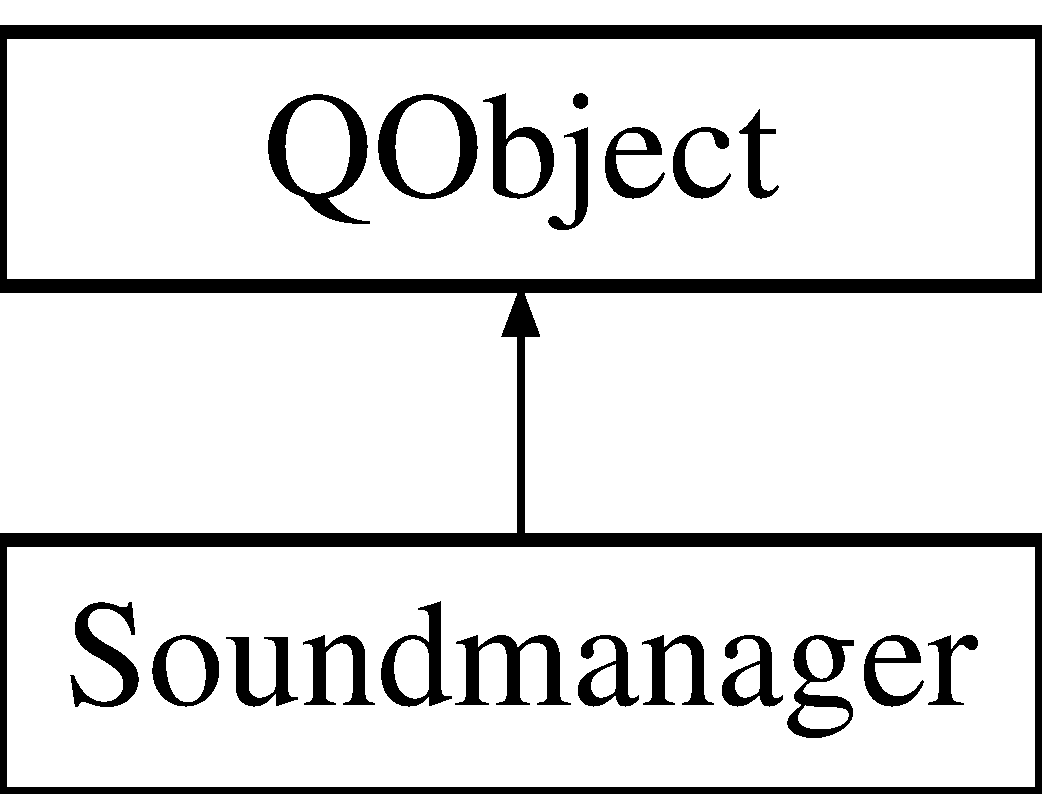
\includegraphics[height=2.000000cm]{class_soundmanager}
\end{center}
\end{figure}
\subsection*{Public Member Functions}
\begin{DoxyCompactItemize}
\item 
virtual \hyperlink{class_soundmanager_a098a604a4cb0a238863ddb0065f11885}{$\sim$\+Soundmanager} ()
\item 
Q\+\_\+\+I\+N\+V\+O\+K\+A\+B\+L\+E void \hyperlink{class_soundmanager_adc77c21e0705c9220b6bfff6d8957d7c}{play\+Background\+Music} ()
\begin{DoxyCompactList}\small\item\em Starts playing our background music. \end{DoxyCompactList}\item 
void \hyperlink{class_soundmanager_a6116af7088ee72cafda5d3e1c6b6600b}{play\+Collision\+Sound} ()
\begin{DoxyCompactList}\small\item\em Plays a previously defined sound in order to indicate a collision. \end{DoxyCompactList}\item 
void \hyperlink{class_soundmanager_a490ddb5b63b94701ad5d246d27759b14}{set\+Collision\+Sound} (\hyperlink{soundmanager_8h_a7fbdfef23a43c911ebc18ef1b9d9808d}{Sound\+Effects} effect)
\begin{DoxyCompactList}\small\item\em Sets the collision sound that will be played next time \hyperlink{class_soundmanager_a6116af7088ee72cafda5d3e1c6b6600b}{play\+Collision\+Sound()} is called. \end{DoxyCompactList}\item 
Q\+\_\+\+I\+N\+V\+O\+K\+A\+B\+L\+E void \hyperlink{class_soundmanager_a36411846ae8c5cd18239cfb913f3dc83}{stop\+Background\+Music} ()
\begin{DoxyCompactList}\small\item\em Stops playing our background music. \end{DoxyCompactList}\end{DoxyCompactItemize}
\subsection*{Static Public Member Functions}
\begin{DoxyCompactItemize}
\item 
static void \hyperlink{class_soundmanager_aa4a2f89d1c517bff42654038da492d65}{drop} ()
\begin{DoxyCompactList}\small\item\em Drops current instance of our \hyperlink{class_soundmanager}{Soundmanager}. \end{DoxyCompactList}\item 
static \hyperlink{class_soundmanager}{Soundmanager} $\ast$ \hyperlink{class_soundmanager_aa1fa87053cd1cd240447a54327962b23}{instance} ()
\begin{DoxyCompactList}\small\item\em The instance of our \hyperlink{class_soundmanager}{Soundmanager}. \end{DoxyCompactList}\end{DoxyCompactItemize}
\subsection*{Protected Member Functions}
\begin{DoxyCompactItemize}
\item 
\hyperlink{class_soundmanager_a8b484955e5732155f07099e53dca61e1}{Soundmanager} ()
\item 
void \hyperlink{class_soundmanager_a97874137f1bc5dcff106b0a5faeca828}{load\+Sounds} ()
\end{DoxyCompactItemize}
\subsection*{Protected Attributes}
\begin{DoxyCompactItemize}
\item 
Q\+Media\+Player $\ast$ \hyperlink{class_soundmanager_a39e32f7d94670486c52e78721a8f4faf}{m\+\_\+background\+Music}
\item 
Q\+Media\+Player $\ast$ \hyperlink{class_soundmanager_a824f9bfdbe61a7db3cb54cb87cb80268}{m\+\_\+collision\+Sound}
\end{DoxyCompactItemize}
\subsection*{Static Protected Attributes}
\begin{DoxyCompactItemize}
\item 
static \hyperlink{class_soundmanager}{Soundmanager} $\ast$ \hyperlink{class_soundmanager_a81105bb352bada9ff056335df0dd2bb3}{m\+\_\+instance} = 0
\end{DoxyCompactItemize}


\subsection{Detailed Description}
The \hyperlink{class_soundmanager}{Soundmanager} class provides several sounds which can be played.  The \hyperlink{class_soundmanager}{Soundmanager} manages the required ressources. 

\subsection{Constructor \& Destructor Documentation}
\hypertarget{class_soundmanager_a098a604a4cb0a238863ddb0065f11885}{}\index{Soundmanager@{Soundmanager}!````~Soundmanager@{$\sim$\+Soundmanager}}
\index{````~Soundmanager@{$\sim$\+Soundmanager}!Soundmanager@{Soundmanager}}
\subsubsection[{$\sim$\+Soundmanager}]{\setlength{\rightskip}{0pt plus 5cm}Soundmanager\+::$\sim$\+Soundmanager (
\begin{DoxyParamCaption}
{}
\end{DoxyParamCaption}
)\hspace{0.3cm}{\ttfamily [virtual]}}\label{class_soundmanager_a098a604a4cb0a238863ddb0065f11885}
\hypertarget{class_soundmanager_a8b484955e5732155f07099e53dca61e1}{}\index{Soundmanager@{Soundmanager}!Soundmanager@{Soundmanager}}
\index{Soundmanager@{Soundmanager}!Soundmanager@{Soundmanager}}
\subsubsection[{Soundmanager}]{\setlength{\rightskip}{0pt plus 5cm}Soundmanager\+::\+Soundmanager (
\begin{DoxyParamCaption}
{}
\end{DoxyParamCaption}
)\hspace{0.3cm}{\ttfamily [protected]}}\label{class_soundmanager_a8b484955e5732155f07099e53dca61e1}


\subsection{Member Function Documentation}
\hypertarget{class_soundmanager_aa4a2f89d1c517bff42654038da492d65}{}\index{Soundmanager@{Soundmanager}!drop@{drop}}
\index{drop@{drop}!Soundmanager@{Soundmanager}}
\subsubsection[{drop}]{\setlength{\rightskip}{0pt plus 5cm}void Soundmanager\+::drop (
\begin{DoxyParamCaption}
{}
\end{DoxyParamCaption}
)\hspace{0.3cm}{\ttfamily [static]}}\label{class_soundmanager_aa4a2f89d1c517bff42654038da492d65}


Drops current instance of our \hyperlink{class_soundmanager}{Soundmanager}. 

\hypertarget{class_soundmanager_aa1fa87053cd1cd240447a54327962b23}{}\index{Soundmanager@{Soundmanager}!instance@{instance}}
\index{instance@{instance}!Soundmanager@{Soundmanager}}
\subsubsection[{instance}]{\setlength{\rightskip}{0pt plus 5cm}{\bf Soundmanager} $\ast$ Soundmanager\+::instance (
\begin{DoxyParamCaption}
{}
\end{DoxyParamCaption}
)\hspace{0.3cm}{\ttfamily [static]}}\label{class_soundmanager_aa1fa87053cd1cd240447a54327962b23}


The instance of our \hyperlink{class_soundmanager}{Soundmanager}. 

\begin{DoxyReturn}{Returns}

\end{DoxyReturn}
\hypertarget{class_soundmanager_a97874137f1bc5dcff106b0a5faeca828}{}\index{Soundmanager@{Soundmanager}!load\+Sounds@{load\+Sounds}}
\index{load\+Sounds@{load\+Sounds}!Soundmanager@{Soundmanager}}
\subsubsection[{load\+Sounds}]{\setlength{\rightskip}{0pt plus 5cm}void Soundmanager\+::load\+Sounds (
\begin{DoxyParamCaption}
{}
\end{DoxyParamCaption}
)\hspace{0.3cm}{\ttfamily [protected]}}\label{class_soundmanager_a97874137f1bc5dcff106b0a5faeca828}
\hypertarget{class_soundmanager_adc77c21e0705c9220b6bfff6d8957d7c}{}\index{Soundmanager@{Soundmanager}!play\+Background\+Music@{play\+Background\+Music}}
\index{play\+Background\+Music@{play\+Background\+Music}!Soundmanager@{Soundmanager}}
\subsubsection[{play\+Background\+Music}]{\setlength{\rightskip}{0pt plus 5cm}void Soundmanager\+::play\+Background\+Music (
\begin{DoxyParamCaption}
{}
\end{DoxyParamCaption}
)}\label{class_soundmanager_adc77c21e0705c9220b6bfff6d8957d7c}


Starts playing our background music. 

\begin{DoxySeeAlso}{See also}
\hyperlink{class_soundmanager_a36411846ae8c5cd18239cfb913f3dc83}{stop\+Background\+Music()} 
\end{DoxySeeAlso}
\hypertarget{class_soundmanager_a6116af7088ee72cafda5d3e1c6b6600b}{}\index{Soundmanager@{Soundmanager}!play\+Collision\+Sound@{play\+Collision\+Sound}}
\index{play\+Collision\+Sound@{play\+Collision\+Sound}!Soundmanager@{Soundmanager}}
\subsubsection[{play\+Collision\+Sound}]{\setlength{\rightskip}{0pt plus 5cm}void Soundmanager\+::play\+Collision\+Sound (
\begin{DoxyParamCaption}
{}
\end{DoxyParamCaption}
)}\label{class_soundmanager_a6116af7088ee72cafda5d3e1c6b6600b}


Plays a previously defined sound in order to indicate a collision. 

\begin{DoxySeeAlso}{See also}
\hyperlink{class_soundmanager_a490ddb5b63b94701ad5d246d27759b14}{set\+Collision\+Sound()} 
\end{DoxySeeAlso}
\hypertarget{class_soundmanager_a490ddb5b63b94701ad5d246d27759b14}{}\index{Soundmanager@{Soundmanager}!set\+Collision\+Sound@{set\+Collision\+Sound}}
\index{set\+Collision\+Sound@{set\+Collision\+Sound}!Soundmanager@{Soundmanager}}
\subsubsection[{set\+Collision\+Sound}]{\setlength{\rightskip}{0pt plus 5cm}void Soundmanager\+::set\+Collision\+Sound (
\begin{DoxyParamCaption}
\item[{{\bf Sound\+Effects}}]{effect}
\end{DoxyParamCaption}
)}\label{class_soundmanager_a490ddb5b63b94701ad5d246d27759b14}


Sets the collision sound that will be played next time \hyperlink{class_soundmanager_a6116af7088ee72cafda5d3e1c6b6600b}{play\+Collision\+Sound()} is called. 


\begin{DoxyParams}{Parameters}
{\em effect} & The choosen Sound\+Effect \\
\hline
\end{DoxyParams}
\hypertarget{class_soundmanager_a36411846ae8c5cd18239cfb913f3dc83}{}\index{Soundmanager@{Soundmanager}!stop\+Background\+Music@{stop\+Background\+Music}}
\index{stop\+Background\+Music@{stop\+Background\+Music}!Soundmanager@{Soundmanager}}
\subsubsection[{stop\+Background\+Music}]{\setlength{\rightskip}{0pt plus 5cm}void Soundmanager\+::stop\+Background\+Music (
\begin{DoxyParamCaption}
{}
\end{DoxyParamCaption}
)}\label{class_soundmanager_a36411846ae8c5cd18239cfb913f3dc83}


Stops playing our background music. 



\subsection{Member Data Documentation}
\hypertarget{class_soundmanager_a39e32f7d94670486c52e78721a8f4faf}{}\index{Soundmanager@{Soundmanager}!m\+\_\+background\+Music@{m\+\_\+background\+Music}}
\index{m\+\_\+background\+Music@{m\+\_\+background\+Music}!Soundmanager@{Soundmanager}}
\subsubsection[{m\+\_\+background\+Music}]{\setlength{\rightskip}{0pt plus 5cm}Q\+Media\+Player$\ast$ Soundmanager\+::m\+\_\+background\+Music\hspace{0.3cm}{\ttfamily [protected]}}\label{class_soundmanager_a39e32f7d94670486c52e78721a8f4faf}
\hypertarget{class_soundmanager_a824f9bfdbe61a7db3cb54cb87cb80268}{}\index{Soundmanager@{Soundmanager}!m\+\_\+collision\+Sound@{m\+\_\+collision\+Sound}}
\index{m\+\_\+collision\+Sound@{m\+\_\+collision\+Sound}!Soundmanager@{Soundmanager}}
\subsubsection[{m\+\_\+collision\+Sound}]{\setlength{\rightskip}{0pt plus 5cm}Q\+Media\+Player$\ast$ Soundmanager\+::m\+\_\+collision\+Sound\hspace{0.3cm}{\ttfamily [protected]}}\label{class_soundmanager_a824f9bfdbe61a7db3cb54cb87cb80268}
\hypertarget{class_soundmanager_a81105bb352bada9ff056335df0dd2bb3}{}\index{Soundmanager@{Soundmanager}!m\+\_\+instance@{m\+\_\+instance}}
\index{m\+\_\+instance@{m\+\_\+instance}!Soundmanager@{Soundmanager}}
\subsubsection[{m\+\_\+instance}]{\setlength{\rightskip}{0pt plus 5cm}{\bf Soundmanager} $\ast$ Soundmanager\+::m\+\_\+instance = 0\hspace{0.3cm}{\ttfamily [static]}, {\ttfamily [protected]}}\label{class_soundmanager_a81105bb352bada9ff056335df0dd2bb3}


The documentation for this class was generated from the following files\+:\begin{DoxyCompactItemize}
\item 
Game-\/\+Programming-\/\+W\+S2014/gem\+Illuminator/\hyperlink{soundmanager_8h}{soundmanager.\+h}\item 
Game-\/\+Programming-\/\+W\+S2014/gem\+Illuminator/\hyperlink{soundmanager_8cpp}{soundmanager.\+cpp}\end{DoxyCompactItemize}

\hypertarget{class_tetrahedron_gem}{}\section{Tetrahedron\+Gem Class Reference}
\label{class_tetrahedron_gem}\index{Tetrahedron\+Gem@{Tetrahedron\+Gem}}


Tetrahedron\+Gems are gems with a shape like a tetrahedron. The only difference to Abstrac\+Gem is the fact, that a \hyperlink{class_tetrahedron_gem}{Tetrahedron\+Gem} has a shape defined.  




{\ttfamily \#include $<$tetrahedrongem.\+h$>$}

Inheritance diagram for Tetrahedron\+Gem\+:\begin{figure}[H]
\begin{center}
\leavevmode
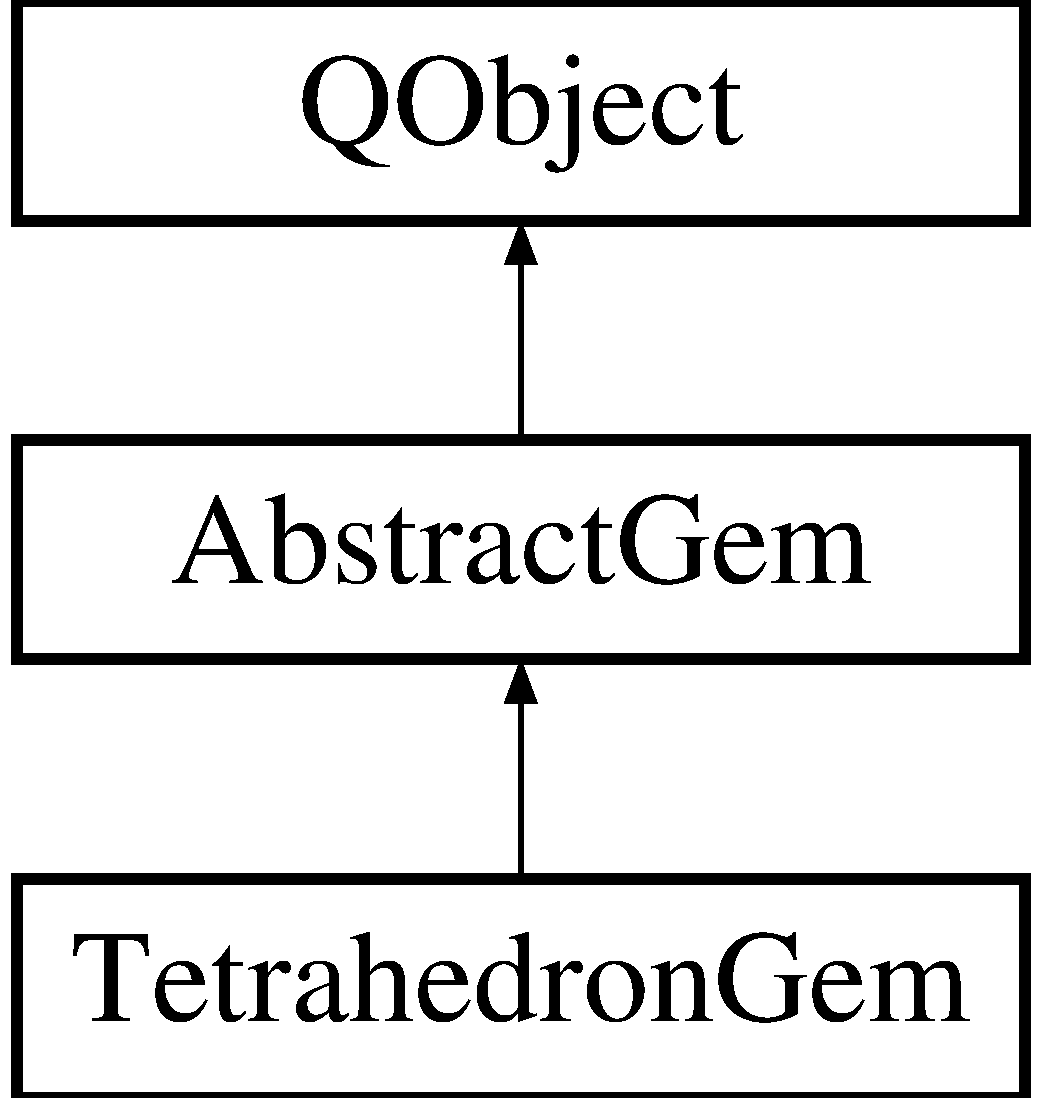
\includegraphics[height=3.000000cm]{class_tetrahedron_gem}
\end{center}
\end{figure}
\subsection*{Public Member Functions}
\begin{DoxyCompactItemize}
\item 
\hyperlink{class_tetrahedron_gem_af942fcb0a4da9b3dfcf989931b2bc393}{Tetrahedron\+Gem} (Q\+Object $\ast$parent=0)
\item 
virtual \hyperlink{class_tetrahedron_gem_ab44903e14715941beda3490914a229ae}{$\sim$\+Tetrahedron\+Gem} ()
\end{DoxyCompactItemize}
\subsection*{Additional Inherited Members}


\subsection{Detailed Description}
Tetrahedron\+Gems are gems with a shape like a tetrahedron. The only difference to Abstrac\+Gem is the fact, that a \hyperlink{class_tetrahedron_gem}{Tetrahedron\+Gem} has a shape defined. 

\subsection{Constructor \& Destructor Documentation}
\hypertarget{class_tetrahedron_gem_af942fcb0a4da9b3dfcf989931b2bc393}{}\index{Tetrahedron\+Gem@{Tetrahedron\+Gem}!Tetrahedron\+Gem@{Tetrahedron\+Gem}}
\index{Tetrahedron\+Gem@{Tetrahedron\+Gem}!Tetrahedron\+Gem@{Tetrahedron\+Gem}}
\subsubsection[{Tetrahedron\+Gem}]{\setlength{\rightskip}{0pt plus 5cm}Tetrahedron\+Gem\+::\+Tetrahedron\+Gem (
\begin{DoxyParamCaption}
\item[{Q\+Object $\ast$}]{parent = {\ttfamily 0}}
\end{DoxyParamCaption}
)\hspace{0.3cm}{\ttfamily [explicit]}}\label{class_tetrahedron_gem_af942fcb0a4da9b3dfcf989931b2bc393}
\hypertarget{class_tetrahedron_gem_ab44903e14715941beda3490914a229ae}{}\index{Tetrahedron\+Gem@{Tetrahedron\+Gem}!````~Tetrahedron\+Gem@{$\sim$\+Tetrahedron\+Gem}}
\index{````~Tetrahedron\+Gem@{$\sim$\+Tetrahedron\+Gem}!Tetrahedron\+Gem@{Tetrahedron\+Gem}}
\subsubsection[{$\sim$\+Tetrahedron\+Gem}]{\setlength{\rightskip}{0pt plus 5cm}Tetrahedron\+Gem\+::$\sim$\+Tetrahedron\+Gem (
\begin{DoxyParamCaption}
{}
\end{DoxyParamCaption}
)\hspace{0.3cm}{\ttfamily [virtual]}}\label{class_tetrahedron_gem_ab44903e14715941beda3490914a229ae}


The documentation for this class was generated from the following files\+:\begin{DoxyCompactItemize}
\item 
Game-\/\+Programming-\/\+W\+S2014/gem\+Illuminator/\hyperlink{tetrahedrongem_8h}{tetrahedrongem.\+h}\item 
Game-\/\+Programming-\/\+W\+S2014/gem\+Illuminator/\hyperlink{tetrahedrongem_8cpp}{tetrahedrongem.\+cpp}\end{DoxyCompactItemize}

\hypertarget{class_triangle}{}\section{Triangle Class Reference}
\label{class_triangle}\index{Triangle@{Triangle}}
\subsection*{Public Member Functions}
\begin{DoxyCompactItemize}
\item 
\hypertarget{class_triangle_ab9220b045480de037944ed99913ecea8}{}{\bfseries Triangle} (\hyperlink{class_abstract_gem}{Abstract\+Gem} $\ast$owning\+Gem)\label{class_triangle_ab9220b045480de037944ed99913ecea8}

\item 
\hypertarget{class_triangle_a860d12ec88ef8821dd10a5a653a7413d}{}{\bfseries Triangle} (const Q\+Vector3\+D \&a, const Q\+Vector3\+D \&b, const Q\+Vector3\+D \&c, \hyperlink{class_abstract_gem}{Abstract\+Gem} $\ast$owning\+Gem)\label{class_triangle_a860d12ec88ef8821dd10a5a653a7413d}

\item 
\hypertarget{class_triangle_a889893fe34e2eb7121082b86199d5628}{}{\bfseries Triangle} (const \hyperlink{class_triangle}{Triangle} \&triangle)\label{class_triangle_a889893fe34e2eb7121082b86199d5628}

\item 
\hypertarget{class_triangle_aae57b61e09898f54256a83e76acfe502}{}\hyperlink{class_triangle}{Triangle} \& {\bfseries operator=} (const \hyperlink{class_triangle}{Triangle} \&triangle)\label{class_triangle_aae57b61e09898f54256a83e76acfe502}

\item 
\hypertarget{class_triangle_a430bf0a9d8eaf20ea7bdefcd8082588c}{}const Q\+Vector3\+D \& {\bfseries a} () const \label{class_triangle_a430bf0a9d8eaf20ea7bdefcd8082588c}

\item 
\hypertarget{class_triangle_a24c012d83d7e6c5d0b27985d8dcb64da}{}void {\bfseries set\+A} (const Q\+Vector3\+D \&a)\label{class_triangle_a24c012d83d7e6c5d0b27985d8dcb64da}

\item 
\hypertarget{class_triangle_a8327124c9b9b752be94187c9fbf3f460}{}const Q\+Vector3\+D \& {\bfseries b} () const \label{class_triangle_a8327124c9b9b752be94187c9fbf3f460}

\item 
\hypertarget{class_triangle_a9f889b49a5ea3b4be4c4366c63673095}{}void {\bfseries set\+B} (const Q\+Vector3\+D \&b)\label{class_triangle_a9f889b49a5ea3b4be4c4366c63673095}

\item 
\hypertarget{class_triangle_a61f6c0245df276555de6d1b1a98840b8}{}const Q\+Vector3\+D \& {\bfseries c} () const \label{class_triangle_a61f6c0245df276555de6d1b1a98840b8}

\item 
\hypertarget{class_triangle_af4566995b306c0f9ae72b457b7acb983}{}void {\bfseries set\+C} (const Q\+Vector3\+D \&c)\label{class_triangle_af4566995b306c0f9ae72b457b7acb983}

\item 
\hypertarget{class_triangle_aa1ccf6af0c2567e53b9dc6f51243f934}{}const Q\+Vector3\+D \& {\bfseries normal} () const \label{class_triangle_aa1ccf6af0c2567e53b9dc6f51243f934}

\item 
\hypertarget{class_triangle_ad51139a1ad219f93031cf1a64646c123}{}Q\+Vector3\+D {\bfseries normalized\+Normal} () const \label{class_triangle_ad51139a1ad219f93031cf1a64646c123}

\item 
\hypertarget{class_triangle_ad29fe2cad14c0285aca2557d3a0c0f13}{}\hyperlink{class_triangle}{Triangle} {\bfseries in\+World\+Coordinates} () const \label{class_triangle_ad29fe2cad14c0285aca2557d3a0c0f13}

\item 
\hypertarget{class_triangle_ae531defb56fd5b0a19078f23954253dc}{}\hyperlink{class_abstract_gem}{Abstract\+Gem} $\ast$ {\bfseries owning\+Gem} () const \label{class_triangle_ae531defb56fd5b0a19078f23954253dc}

\item 
\hypertarget{class_triangle_a66da12d2c747c435ea5148df472d9229}{}\hyperlink{class_q_list}{Q\+List}$<$ Q\+Vector3\+D $>$ {\bfseries vertices} () const \label{class_triangle_a66da12d2c747c435ea5148df472d9229}

\item 
\hypertarget{class_triangle_a4fb81ac7e355c97a03f4c056bd79ac99}{}Q\+Vector3\+D {\bfseries reflect} (const Q\+Vector3\+D \&incident\+Vector) const \label{class_triangle_a4fb81ac7e355c97a03f4c056bd79ac99}

\end{DoxyCompactItemize}
\subsection*{Protected Member Functions}
\begin{DoxyCompactItemize}
\item 
\hypertarget{class_triangle_a429f86c999f5c27720f7b912fa3b20ca}{}void {\bfseries calculate\+Normal} () const \label{class_triangle_a429f86c999f5c27720f7b912fa3b20ca}

\end{DoxyCompactItemize}
\subsection*{Protected Attributes}
\begin{DoxyCompactItemize}
\item 
\hypertarget{class_triangle_a38f859bd8a6291d1fe460dbcf3c937c8}{}Q\+Vector3\+D $\ast$ {\bfseries m\+\_\+a}\label{class_triangle_a38f859bd8a6291d1fe460dbcf3c937c8}

\item 
\hypertarget{class_triangle_a783a7fcacbfa566c37dfd3fa8c6f44fd}{}Q\+Vector3\+D $\ast$ {\bfseries m\+\_\+b}\label{class_triangle_a783a7fcacbfa566c37dfd3fa8c6f44fd}

\item 
\hypertarget{class_triangle_ae39dcbf0b28b543900380517bbef628c}{}Q\+Vector3\+D $\ast$ {\bfseries m\+\_\+c}\label{class_triangle_ae39dcbf0b28b543900380517bbef628c}

\item 
\hypertarget{class_triangle_a86922a6a07e847f2df3b9310af273d8a}{}Q\+Vector3\+D $\ast$ {\bfseries m\+\_\+normal}\label{class_triangle_a86922a6a07e847f2df3b9310af273d8a}

\item 
\hypertarget{class_triangle_a205c63aa77abccf049d3535cb2512df0}{}\hyperlink{class_abstract_gem}{Abstract\+Gem} $\ast$ {\bfseries m\+\_\+gem}\label{class_triangle_a205c63aa77abccf049d3535cb2512df0}

\end{DoxyCompactItemize}


The documentation for this class was generated from the following files\+:\begin{DoxyCompactItemize}
\item 
gem\+Illuminator/triangle.\+h\item 
gem\+Illuminator/triangle.\+cpp\end{DoxyCompactItemize}

\chapter{File Documentation}
\hypertarget{abstractgem_8cpp}{\section{abstractgem.\+cpp File Reference}
\label{abstractgem_8cpp}\index{abstractgem.\+cpp@{abstractgem.\+cpp}}
}
{\ttfamily \#include \char`\"{}abstractgem.\+h\char`\"{}}\\*
{\ttfamily \#include $<$limits$>$}\\*
{\ttfamily \#include $<$Q\+Quaternion$>$}\\*
{\ttfamily \#include $<$Q\+Matrix4x4$>$}\\*
{\ttfamily \#include \char`\"{}gemdata.\+h\char`\"{}}\\*
{\ttfamily \#include \char`\"{}lightray.\+h\char`\"{}}\\*
{\ttfamily \#include \char`\"{}triangle.\+h\char`\"{}}\\*
{\ttfamily \#include \char`\"{}scene.\+h\char`\"{}}\\*
\subsection*{Functions}
\begin{DoxyCompactItemize}
\item 
Q\+Vector3\+D \hyperlink{abstractgem_8cpp_a697c6102488dd3c0aff0ca9ddccf23cd}{rotate\+Vector} (const Q\+Vector3\+D \&vector, const Q\+Quaternion \&quaternion)
\item 
uint \hyperlink{abstractgem_8cpp_a92fb5a3a6f53f07f0f9653dd299d31ff}{q\+Hash} (\hyperlink{abstractgem_8h_a2f0a34b6dac35a9610cab7a1c5fcb444}{Gem\+Type} key, uint seed)
\begin{DoxyCompactList}\small\item\em Custom implementation of q\+Hash. Providing hash calculation for Gem\+Type. In order to use Gem\+Type as key in \hyperlink{singleton_q_hash}{Q\+Hash} and \hyperlink{singleton_q_set}{Q\+Set}. \end{DoxyCompactList}\end{DoxyCompactItemize}


\subsection{Function Documentation}
\hypertarget{abstractgem_8cpp_a92fb5a3a6f53f07f0f9653dd299d31ff}{\index{abstractgem.\+cpp@{abstractgem.\+cpp}!q\+Hash@{q\+Hash}}
\index{q\+Hash@{q\+Hash}!abstractgem.\+cpp@{abstractgem.\+cpp}}
\subsubsection[{q\+Hash}]{\setlength{\rightskip}{0pt plus 5cm}uint q\+Hash (
\begin{DoxyParamCaption}
\item[{{\bf Gem\+Type}}]{key, }
\item[{uint}]{seed}
\end{DoxyParamCaption}
)}}\label{abstractgem_8cpp_a92fb5a3a6f53f07f0f9653dd299d31ff}


Custom implementation of q\+Hash. Providing hash calculation for Gem\+Type. In order to use Gem\+Type as key in \hyperlink{singleton_q_hash}{Q\+Hash} and \hyperlink{singleton_q_set}{Q\+Set}. 


\begin{DoxyParams}{Parameters}
{\em key} & Value the hash value is calculated for \\
\hline
{\em seed} & \\
\hline
\end{DoxyParams}
\begin{DoxyReturn}{Returns}
Returns hash value. 
\end{DoxyReturn}
\hypertarget{abstractgem_8cpp_a697c6102488dd3c0aff0ca9ddccf23cd}{\index{abstractgem.\+cpp@{abstractgem.\+cpp}!rotate\+Vector@{rotate\+Vector}}
\index{rotate\+Vector@{rotate\+Vector}!abstractgem.\+cpp@{abstractgem.\+cpp}}
\subsubsection[{rotate\+Vector}]{\setlength{\rightskip}{0pt plus 5cm}Q\+Vector3\+D rotate\+Vector (
\begin{DoxyParamCaption}
\item[{const Q\+Vector3\+D \&}]{vector, }
\item[{const Q\+Quaternion \&}]{quaternion}
\end{DoxyParamCaption}
)}}\label{abstractgem_8cpp_a697c6102488dd3c0aff0ca9ddccf23cd}

\hypertarget{abstractgem_8h}{}\section{Game-\/\+Programming-\/\+W\+S2014/gem\+Illuminator/abstractgem.h File Reference}
\label{abstractgem_8h}\index{Game-\/\+Programming-\/\+W\+S2014/gem\+Illuminator/abstractgem.\+h@{Game-\/\+Programming-\/\+W\+S2014/gem\+Illuminator/abstractgem.\+h}}
{\ttfamily \#include $<$Q\+Object$>$}\\*
{\ttfamily \#include $<$Q\+Quaternion$>$}\\*
{\ttfamily \#include $<$Q\+Vector3\+D$>$}\\*
\subsection*{Classes}
\begin{DoxyCompactItemize}
\item 
class \hyperlink{class_abstract_gem}{Abstract\+Gem}
\begin{DoxyCompactList}\small\item\em The \hyperlink{class_abstract_gem}{Abstract\+Gem} class is our base class of all gems.  As base class all required information of a gem are stored. Also usefull algorithms for collision detection are provided. Furthermore this class is supposed to be used within Q\+M\+L. \end{DoxyCompactList}\end{DoxyCompactItemize}
\subsection*{Enumerations}
\begin{DoxyCompactItemize}
\item 
enum \hyperlink{abstractgem_8h_a2f0a34b6dac35a9610cab7a1c5fcb444}{Gem\+Type} \{ \hyperlink{abstractgem_8h_a2f0a34b6dac35a9610cab7a1c5fcb444ae353dbe42c8654f33588d4da0b517469}{Gem\+Type\+::\+Abstract}, 
\hyperlink{abstractgem_8h_a2f0a34b6dac35a9610cab7a1c5fcb444aa296104f0c61a9cf39f4824d05315e12}{Gem\+Type\+::\+Cube}, 
\hyperlink{abstractgem_8h_a2f0a34b6dac35a9610cab7a1c5fcb444ae029cf63d8d01a489974f9289b50dc80}{Gem\+Type\+::\+Tetrahedron}
 \}
\begin{DoxyCompactList}\small\item\em The Gem\+Type An enum describing current gem type. This enum is used for faster comparision of gems, because all gems of one type have same (objectspace) vertices. \end{DoxyCompactList}\end{DoxyCompactItemize}
\subsection*{Functions}
\begin{DoxyCompactItemize}
\item 
uint \hyperlink{abstractgem_8h_a92fb5a3a6f53f07f0f9653dd299d31ff}{q\+Hash} (\hyperlink{abstractgem_8h_a2f0a34b6dac35a9610cab7a1c5fcb444}{Gem\+Type} key, uint seed)
\begin{DoxyCompactList}\small\item\em Custom implementation of q\+Hash. Providing hash calculation for Gem\+Type. In order to use Gem\+Type as key in \hyperlink{class_q_hash}{Q\+Hash} and \hyperlink{class_q_set}{Q\+Set}. \end{DoxyCompactList}\end{DoxyCompactItemize}


\subsection{Enumeration Type Documentation}
\hypertarget{abstractgem_8h_a2f0a34b6dac35a9610cab7a1c5fcb444}{}\index{abstractgem.\+h@{abstractgem.\+h}!Gem\+Type@{Gem\+Type}}
\index{Gem\+Type@{Gem\+Type}!abstractgem.\+h@{abstractgem.\+h}}
\subsubsection[{Gem\+Type}]{\setlength{\rightskip}{0pt plus 5cm}enum {\bf Gem\+Type}\hspace{0.3cm}{\ttfamily [strong]}}\label{abstractgem_8h_a2f0a34b6dac35a9610cab7a1c5fcb444}


The Gem\+Type An enum describing current gem type. This enum is used for faster comparision of gems, because all gems of one type have same (objectspace) vertices. 

\begin{Desc}
\item[Enumerator]\par
\begin{description}
\index{Abstract@{Abstract}!abstractgem.\+h@{abstractgem.\+h}}\index{abstractgem.\+h@{abstractgem.\+h}!Abstract@{Abstract}}\item[{\em 
\hypertarget{abstractgem_8h_a2f0a34b6dac35a9610cab7a1c5fcb444ae353dbe42c8654f33588d4da0b517469}{}Abstract\label{abstractgem_8h_a2f0a34b6dac35a9610cab7a1c5fcb444ae353dbe42c8654f33588d4da0b517469}
}]\index{Cube@{Cube}!abstractgem.\+h@{abstractgem.\+h}}\index{abstractgem.\+h@{abstractgem.\+h}!Cube@{Cube}}\item[{\em 
\hypertarget{abstractgem_8h_a2f0a34b6dac35a9610cab7a1c5fcb444aa296104f0c61a9cf39f4824d05315e12}{}Cube\label{abstractgem_8h_a2f0a34b6dac35a9610cab7a1c5fcb444aa296104f0c61a9cf39f4824d05315e12}
}]\index{Tetrahedron@{Tetrahedron}!abstractgem.\+h@{abstractgem.\+h}}\index{abstractgem.\+h@{abstractgem.\+h}!Tetrahedron@{Tetrahedron}}\item[{\em 
\hypertarget{abstractgem_8h_a2f0a34b6dac35a9610cab7a1c5fcb444ae029cf63d8d01a489974f9289b50dc80}{}Tetrahedron\label{abstractgem_8h_a2f0a34b6dac35a9610cab7a1c5fcb444ae029cf63d8d01a489974f9289b50dc80}
}]\end{description}
\end{Desc}


\subsection{Function Documentation}
\hypertarget{abstractgem_8h_a92fb5a3a6f53f07f0f9653dd299d31ff}{}\index{abstractgem.\+h@{abstractgem.\+h}!q\+Hash@{q\+Hash}}
\index{q\+Hash@{q\+Hash}!abstractgem.\+h@{abstractgem.\+h}}
\subsubsection[{q\+Hash}]{\setlength{\rightskip}{0pt plus 5cm}uint q\+Hash (
\begin{DoxyParamCaption}
\item[{{\bf Gem\+Type}}]{key, }
\item[{uint}]{seed}
\end{DoxyParamCaption}
)}\label{abstractgem_8h_a92fb5a3a6f53f07f0f9653dd299d31ff}


Custom implementation of q\+Hash. Providing hash calculation for Gem\+Type. In order to use Gem\+Type as key in \hyperlink{class_q_hash}{Q\+Hash} and \hyperlink{class_q_set}{Q\+Set}. 


\begin{DoxyParams}{Parameters}
{\em key} & Value the hash value is calculated for \\
\hline
{\em seed} & \\
\hline
\end{DoxyParams}
\begin{DoxyReturn}{Returns}
Returns hash value. 
\end{DoxyReturn}

\hypertarget{_qt_activity_8java}{\section{android/src/org/qtproject/qt5/android/bindings/\+Qt\+Activity.java File Reference}
\label{_qt_activity_8java}\index{android/src/org/qtproject/qt5/android/bindings/\+Qt\+Activity.\+java@{android/src/org/qtproject/qt5/android/bindings/\+Qt\+Activity.\+java}}
}
\subsection*{Classes}
\begin{DoxyCompactItemize}
\item 
class \hyperlink{classorg_1_1qtproject_1_1qt5_1_1android_1_1bindings_1_1_qt_activity}{org.\+qtproject.\+qt5.\+android.\+bindings.\+Qt\+Activity}
\end{DoxyCompactItemize}
\subsection*{Packages}
\begin{DoxyCompactItemize}
\item 
package \hyperlink{namespaceorg_1_1qtproject_1_1qt5_1_1android_1_1bindings}{org.\+qtproject.\+qt5.\+android.\+bindings}
\end{DoxyCompactItemize}

\hypertarget{blureffect_8cpp}{\section{blureffect.\+cpp File Reference}
\label{blureffect_8cpp}\index{blureffect.\+cpp@{blureffect.\+cpp}}
}
{\ttfamily \#include \char`\"{}blureffect.\+h\char`\"{}}\\*
{\ttfamily \#include $<$Q\+Map$>$}\\*
{\ttfamily \#include $<$Q\+Open\+G\+L\+Functions$>$}\\*
{\ttfamily \#include $<$Q\+Open\+G\+L\+Shader\+Program$>$}\\*
{\ttfamily \#include $<$Q\+Size$>$}\\*
{\ttfamily \#include \char`\"{}screenalignedquad.\+h\char`\"{}}\\*
{\ttfamily \#include \char`\"{}shaderprograms.\+h\char`\"{}}\\*

\hypertarget{blureffect_8h}{}\section{Game-\/\+Programming-\/\+W\+S2014/gem\+Illuminator/blureffect.h File Reference}
\label{blureffect_8h}\index{Game-\/\+Programming-\/\+W\+S2014/gem\+Illuminator/blureffect.\+h@{Game-\/\+Programming-\/\+W\+S2014/gem\+Illuminator/blureffect.\+h}}
{\ttfamily \#include $<$Q\+Object$>$}\\*
\subsection*{Classes}
\begin{DoxyCompactItemize}
\item 
class \hyperlink{class_blur_effect}{Blur\+Effect}
\begin{DoxyCompactList}\small\item\em The \hyperlink{class_blur_effect}{Blur\+Effect} blurs a given texture. \end{DoxyCompactList}\end{DoxyCompactItemize}

\hypertarget{moc__abstractgeometry_8cpp}{\section{build-\/\+Gem\+Illuminator-\/\+Desktop\+\_\+\+Qt\+\_\+5\+\_\+3\+\_\+\+M\+S\+V\+C2013\+\_\+\+Open\+G\+L\+\_\+64bit-\/\+Debug/debug/moc\+\_\+abstractgeometry.cpp File Reference}
\label{moc__abstractgeometry_8cpp}\index{build-\/\+Gem\+Illuminator-\/\+Desktop\+\_\+\+Qt\+\_\+5\+\_\+3\+\_\+\+M\+S\+V\+C2013\+\_\+\+Open\+G\+L\+\_\+64bit-\/\+Debug/debug/moc\+\_\+abstractgeometry.\+cpp@{build-\/\+Gem\+Illuminator-\/\+Desktop\+\_\+\+Qt\+\_\+5\+\_\+3\+\_\+\+M\+S\+V\+C2013\+\_\+\+Open\+G\+L\+\_\+64bit-\/\+Debug/debug/moc\+\_\+abstractgeometry.\+cpp}}
}
{\ttfamily \#include \char`\"{}../../\+Gem\+Illuminator/abstractgeometry.\+h\char`\"{}}\\*
{\ttfamily \#include $<$Qt\+Core/qbytearray.\+h$>$}\\*
{\ttfamily \#include $<$Qt\+Core/qmetatype.\+h$>$}\\*
\subsection*{Classes}
\begin{DoxyCompactItemize}
\item 
struct \hyperlink{structqt__meta__stringdata___abstract_geometry__t}{qt\+\_\+meta\+\_\+stringdata\+\_\+\+Abstract\+Geometry\+\_\+t}
\end{DoxyCompactItemize}
\subsection*{Macros}
\begin{DoxyCompactItemize}
\item 
\#define \hyperlink{moc__abstractgeometry_8cpp_a75bb9482d242cde0a06c9dbdc6b83abe}{Q\+T\+\_\+\+M\+O\+C\+\_\+\+L\+I\+T\+E\+R\+A\+L}(idx, ofs, len)
\end{DoxyCompactItemize}


\subsection{Macro Definition Documentation}
\hypertarget{moc__abstractgeometry_8cpp_a75bb9482d242cde0a06c9dbdc6b83abe}{\index{moc\+\_\+abstractgeometry.\+cpp@{moc\+\_\+abstractgeometry.\+cpp}!Q\+T\+\_\+\+M\+O\+C\+\_\+\+L\+I\+T\+E\+R\+A\+L@{Q\+T\+\_\+\+M\+O\+C\+\_\+\+L\+I\+T\+E\+R\+A\+L}}
\index{Q\+T\+\_\+\+M\+O\+C\+\_\+\+L\+I\+T\+E\+R\+A\+L@{Q\+T\+\_\+\+M\+O\+C\+\_\+\+L\+I\+T\+E\+R\+A\+L}!moc\+\_\+abstractgeometry.\+cpp@{moc\+\_\+abstractgeometry.\+cpp}}
\subsubsection[{Q\+T\+\_\+\+M\+O\+C\+\_\+\+L\+I\+T\+E\+R\+A\+L}]{\setlength{\rightskip}{0pt plus 5cm}\#define Q\+T\+\_\+\+M\+O\+C\+\_\+\+L\+I\+T\+E\+R\+A\+L(
\begin{DoxyParamCaption}
\item[{}]{idx, }
\item[{}]{ofs, }
\item[{}]{len}
\end{DoxyParamCaption}
)}}\label{moc__abstractgeometry_8cpp_a75bb9482d242cde0a06c9dbdc6b83abe}
{\bfseries Value\+:}
\begin{DoxyCode}
Q\_STATIC\_BYTE\_ARRAY\_DATA\_HEADER\_INITIALIZER\_WITH\_OFFSET(len, \(\backslash\)
    qptrdiff(offsetof(\hyperlink{structqt__meta__stringdata___abstract_geometry__t}{qt\_meta\_stringdata\_AbstractGeometry\_t}, 
      stringdata) + ofs \(\backslash\)
        - idx * \textcolor{keyword}{sizeof}(QByteArrayData)) \(\backslash\)
    )
\end{DoxyCode}

\hypertarget{moc__abstractgeometryrenderer_8cpp}{\section{build-\/\+Gem\+Illuminator-\/\+Desktop\+\_\+\+Qt\+\_\+5\+\_\+3\+\_\+\+M\+S\+V\+C2013\+\_\+\+Open\+G\+L\+\_\+64bit-\/\+Debug/debug/moc\+\_\+abstractgeometryrenderer.cpp File Reference}
\label{moc__abstractgeometryrenderer_8cpp}\index{build-\/\+Gem\+Illuminator-\/\+Desktop\+\_\+\+Qt\+\_\+5\+\_\+3\+\_\+\+M\+S\+V\+C2013\+\_\+\+Open\+G\+L\+\_\+64bit-\/\+Debug/debug/moc\+\_\+abstractgeometryrenderer.\+cpp@{build-\/\+Gem\+Illuminator-\/\+Desktop\+\_\+\+Qt\+\_\+5\+\_\+3\+\_\+\+M\+S\+V\+C2013\+\_\+\+Open\+G\+L\+\_\+64bit-\/\+Debug/debug/moc\+\_\+abstractgeometryrenderer.\+cpp}}
}
{\ttfamily \#include \char`\"{}../../\+Gem\+Illuminator/abstractgeometryrenderer.\+h\char`\"{}}\\*
{\ttfamily \#include $<$Qt\+Core/qbytearray.\+h$>$}\\*
{\ttfamily \#include $<$Qt\+Core/qmetatype.\+h$>$}\\*
\subsection*{Classes}
\begin{DoxyCompactItemize}
\item 
struct \hyperlink{structqt__meta__stringdata___abstract_geometry_renderer__t}{qt\+\_\+meta\+\_\+stringdata\+\_\+\+Abstract\+Geometry\+Renderer\+\_\+t}
\end{DoxyCompactItemize}
\subsection*{Macros}
\begin{DoxyCompactItemize}
\item 
\#define \hyperlink{moc__abstractgeometryrenderer_8cpp_a75bb9482d242cde0a06c9dbdc6b83abe}{Q\+T\+\_\+\+M\+O\+C\+\_\+\+L\+I\+T\+E\+R\+A\+L}(idx, ofs, len)
\end{DoxyCompactItemize}


\subsection{Macro Definition Documentation}
\hypertarget{moc__abstractgeometryrenderer_8cpp_a75bb9482d242cde0a06c9dbdc6b83abe}{\index{moc\+\_\+abstractgeometryrenderer.\+cpp@{moc\+\_\+abstractgeometryrenderer.\+cpp}!Q\+T\+\_\+\+M\+O\+C\+\_\+\+L\+I\+T\+E\+R\+A\+L@{Q\+T\+\_\+\+M\+O\+C\+\_\+\+L\+I\+T\+E\+R\+A\+L}}
\index{Q\+T\+\_\+\+M\+O\+C\+\_\+\+L\+I\+T\+E\+R\+A\+L@{Q\+T\+\_\+\+M\+O\+C\+\_\+\+L\+I\+T\+E\+R\+A\+L}!moc\+\_\+abstractgeometryrenderer.\+cpp@{moc\+\_\+abstractgeometryrenderer.\+cpp}}
\subsubsection[{Q\+T\+\_\+\+M\+O\+C\+\_\+\+L\+I\+T\+E\+R\+A\+L}]{\setlength{\rightskip}{0pt plus 5cm}\#define Q\+T\+\_\+\+M\+O\+C\+\_\+\+L\+I\+T\+E\+R\+A\+L(
\begin{DoxyParamCaption}
\item[{}]{idx, }
\item[{}]{ofs, }
\item[{}]{len}
\end{DoxyParamCaption}
)}}\label{moc__abstractgeometryrenderer_8cpp_a75bb9482d242cde0a06c9dbdc6b83abe}
{\bfseries Value\+:}
\begin{DoxyCode}
Q\_STATIC\_BYTE\_ARRAY\_DATA\_HEADER\_INITIALIZER\_WITH\_OFFSET(len, \(\backslash\)
    qptrdiff(offsetof(\hyperlink{structqt__meta__stringdata___abstract_geometry_renderer__t}{qt\_meta\_stringdata\_AbstractGeometryRenderer\_t}
      , stringdata) + ofs \(\backslash\)
        - idx * \textcolor{keyword}{sizeof}(QByteArrayData)) \(\backslash\)
    )
\end{DoxyCode}

\hypertarget{moc__abstractnavigation_8cpp}{\section{build-\/\+Gem\+Illuminator-\/\+Desktop\+\_\+\+Qt\+\_\+5\+\_\+3\+\_\+\+M\+S\+V\+C2013\+\_\+\+Open\+G\+L\+\_\+64bit-\/\+Debug/debug/moc\+\_\+abstractnavigation.cpp File Reference}
\label{moc__abstractnavigation_8cpp}\index{build-\/\+Gem\+Illuminator-\/\+Desktop\+\_\+\+Qt\+\_\+5\+\_\+3\+\_\+\+M\+S\+V\+C2013\+\_\+\+Open\+G\+L\+\_\+64bit-\/\+Debug/debug/moc\+\_\+abstractnavigation.\+cpp@{build-\/\+Gem\+Illuminator-\/\+Desktop\+\_\+\+Qt\+\_\+5\+\_\+3\+\_\+\+M\+S\+V\+C2013\+\_\+\+Open\+G\+L\+\_\+64bit-\/\+Debug/debug/moc\+\_\+abstractnavigation.\+cpp}}
}
{\ttfamily \#include \char`\"{}../../\+Gem\+Illuminator/abstractnavigation.\+h\char`\"{}}\\*
{\ttfamily \#include $<$Qt\+Core/qbytearray.\+h$>$}\\*
{\ttfamily \#include $<$Qt\+Core/qmetatype.\+h$>$}\\*
\subsection*{Classes}
\begin{DoxyCompactItemize}
\item 
struct \hyperlink{structqt__meta__stringdata___abstract_navigation__t}{qt\+\_\+meta\+\_\+stringdata\+\_\+\+Abstract\+Navigation\+\_\+t}
\end{DoxyCompactItemize}
\subsection*{Macros}
\begin{DoxyCompactItemize}
\item 
\#define \hyperlink{moc__abstractnavigation_8cpp_a75bb9482d242cde0a06c9dbdc6b83abe}{Q\+T\+\_\+\+M\+O\+C\+\_\+\+L\+I\+T\+E\+R\+A\+L}(idx, ofs, len)
\end{DoxyCompactItemize}


\subsection{Macro Definition Documentation}
\hypertarget{moc__abstractnavigation_8cpp_a75bb9482d242cde0a06c9dbdc6b83abe}{\index{moc\+\_\+abstractnavigation.\+cpp@{moc\+\_\+abstractnavigation.\+cpp}!Q\+T\+\_\+\+M\+O\+C\+\_\+\+L\+I\+T\+E\+R\+A\+L@{Q\+T\+\_\+\+M\+O\+C\+\_\+\+L\+I\+T\+E\+R\+A\+L}}
\index{Q\+T\+\_\+\+M\+O\+C\+\_\+\+L\+I\+T\+E\+R\+A\+L@{Q\+T\+\_\+\+M\+O\+C\+\_\+\+L\+I\+T\+E\+R\+A\+L}!moc\+\_\+abstractnavigation.\+cpp@{moc\+\_\+abstractnavigation.\+cpp}}
\subsubsection[{Q\+T\+\_\+\+M\+O\+C\+\_\+\+L\+I\+T\+E\+R\+A\+L}]{\setlength{\rightskip}{0pt plus 5cm}\#define Q\+T\+\_\+\+M\+O\+C\+\_\+\+L\+I\+T\+E\+R\+A\+L(
\begin{DoxyParamCaption}
\item[{}]{idx, }
\item[{}]{ofs, }
\item[{}]{len}
\end{DoxyParamCaption}
)}}\label{moc__abstractnavigation_8cpp_a75bb9482d242cde0a06c9dbdc6b83abe}
{\bfseries Value\+:}
\begin{DoxyCode}
Q\_STATIC\_BYTE\_ARRAY\_DATA\_HEADER\_INITIALIZER\_WITH\_OFFSET(len, \(\backslash\)
    qptrdiff(offsetof(\hyperlink{structqt__meta__stringdata___abstract_navigation__t}{qt\_meta\_stringdata\_AbstractNavigation\_t}, 
      stringdata) + ofs \(\backslash\)
        - idx * \textcolor{keyword}{sizeof}(QByteArrayData)) \(\backslash\)
    )
\end{DoxyCode}

\hypertarget{moc__lightray_8cpp}{\section{build-\/\+Gem\+Illuminator-\/\+Desktop\+\_\+\+Qt\+\_\+5\+\_\+3\+\_\+\+M\+S\+V\+C2013\+\_\+\+Open\+G\+L\+\_\+64bit-\/\+Debug/debug/moc\+\_\+lightray.cpp File Reference}
\label{moc__lightray_8cpp}\index{build-\/\+Gem\+Illuminator-\/\+Desktop\+\_\+\+Qt\+\_\+5\+\_\+3\+\_\+\+M\+S\+V\+C2013\+\_\+\+Open\+G\+L\+\_\+64bit-\/\+Debug/debug/moc\+\_\+lightray.\+cpp@{build-\/\+Gem\+Illuminator-\/\+Desktop\+\_\+\+Qt\+\_\+5\+\_\+3\+\_\+\+M\+S\+V\+C2013\+\_\+\+Open\+G\+L\+\_\+64bit-\/\+Debug/debug/moc\+\_\+lightray.\+cpp}}
}
{\ttfamily \#include \char`\"{}../../\+Gem\+Illuminator/lightray.\+h\char`\"{}}\\*
{\ttfamily \#include $<$Qt\+Core/qbytearray.\+h$>$}\\*
{\ttfamily \#include $<$Qt\+Core/qmetatype.\+h$>$}\\*
\subsection*{Classes}
\begin{DoxyCompactItemize}
\item 
struct \hyperlink{structqt__meta__stringdata___light_ray__t}{qt\+\_\+meta\+\_\+stringdata\+\_\+\+Light\+Ray\+\_\+t}
\end{DoxyCompactItemize}
\subsection*{Macros}
\begin{DoxyCompactItemize}
\item 
\#define \hyperlink{moc__lightray_8cpp_a75bb9482d242cde0a06c9dbdc6b83abe}{Q\+T\+\_\+\+M\+O\+C\+\_\+\+L\+I\+T\+E\+R\+A\+L}(idx, ofs, len)
\end{DoxyCompactItemize}


\subsection{Macro Definition Documentation}
\hypertarget{moc__lightray_8cpp_a75bb9482d242cde0a06c9dbdc6b83abe}{\index{moc\+\_\+lightray.\+cpp@{moc\+\_\+lightray.\+cpp}!Q\+T\+\_\+\+M\+O\+C\+\_\+\+L\+I\+T\+E\+R\+A\+L@{Q\+T\+\_\+\+M\+O\+C\+\_\+\+L\+I\+T\+E\+R\+A\+L}}
\index{Q\+T\+\_\+\+M\+O\+C\+\_\+\+L\+I\+T\+E\+R\+A\+L@{Q\+T\+\_\+\+M\+O\+C\+\_\+\+L\+I\+T\+E\+R\+A\+L}!moc\+\_\+lightray.\+cpp@{moc\+\_\+lightray.\+cpp}}
\subsubsection[{Q\+T\+\_\+\+M\+O\+C\+\_\+\+L\+I\+T\+E\+R\+A\+L}]{\setlength{\rightskip}{0pt plus 5cm}\#define Q\+T\+\_\+\+M\+O\+C\+\_\+\+L\+I\+T\+E\+R\+A\+L(
\begin{DoxyParamCaption}
\item[{}]{idx, }
\item[{}]{ofs, }
\item[{}]{len}
\end{DoxyParamCaption}
)}}\label{moc__lightray_8cpp_a75bb9482d242cde0a06c9dbdc6b83abe}
{\bfseries Value\+:}
\begin{DoxyCode}
Q\_STATIC\_BYTE\_ARRAY\_DATA\_HEADER\_INITIALIZER\_WITH\_OFFSET(len, \(\backslash\)
    qptrdiff(offsetof(\hyperlink{structqt__meta__stringdata___light_ray__t}{qt\_meta\_stringdata\_LightRay\_t}, stringdata) + ofs \(\backslash\)
        - idx * \textcolor{keyword}{sizeof}(QByteArrayData)) \(\backslash\)
    )
\end{DoxyCode}

\hypertarget{moc__player_8cpp}{\section{build-\/\+Gem\+Illuminator-\/\+Desktop\+\_\+\+Qt\+\_\+5\+\_\+3\+\_\+\+M\+S\+V\+C2013\+\_\+\+Open\+G\+L\+\_\+64bit-\/\+Debug/debug/moc\+\_\+player.cpp File Reference}
\label{moc__player_8cpp}\index{build-\/\+Gem\+Illuminator-\/\+Desktop\+\_\+\+Qt\+\_\+5\+\_\+3\+\_\+\+M\+S\+V\+C2013\+\_\+\+Open\+G\+L\+\_\+64bit-\/\+Debug/debug/moc\+\_\+player.\+cpp@{build-\/\+Gem\+Illuminator-\/\+Desktop\+\_\+\+Qt\+\_\+5\+\_\+3\+\_\+\+M\+S\+V\+C2013\+\_\+\+Open\+G\+L\+\_\+64bit-\/\+Debug/debug/moc\+\_\+player.\+cpp}}
}
{\ttfamily \#include \char`\"{}../../\+Gem\+Illuminator/player.\+h\char`\"{}}\\*
{\ttfamily \#include $<$Qt\+Core/qbytearray.\+h$>$}\\*
{\ttfamily \#include $<$Qt\+Core/qmetatype.\+h$>$}\\*
\subsection*{Classes}
\begin{DoxyCompactItemize}
\item 
struct \hyperlink{structqt__meta__stringdata___player__t}{qt\+\_\+meta\+\_\+stringdata\+\_\+\+Player\+\_\+t}
\end{DoxyCompactItemize}
\subsection*{Macros}
\begin{DoxyCompactItemize}
\item 
\#define \hyperlink{moc__player_8cpp_a75bb9482d242cde0a06c9dbdc6b83abe}{Q\+T\+\_\+\+M\+O\+C\+\_\+\+L\+I\+T\+E\+R\+A\+L}(idx, ofs, len)
\end{DoxyCompactItemize}


\subsection{Macro Definition Documentation}
\hypertarget{moc__player_8cpp_a75bb9482d242cde0a06c9dbdc6b83abe}{\index{moc\+\_\+player.\+cpp@{moc\+\_\+player.\+cpp}!Q\+T\+\_\+\+M\+O\+C\+\_\+\+L\+I\+T\+E\+R\+A\+L@{Q\+T\+\_\+\+M\+O\+C\+\_\+\+L\+I\+T\+E\+R\+A\+L}}
\index{Q\+T\+\_\+\+M\+O\+C\+\_\+\+L\+I\+T\+E\+R\+A\+L@{Q\+T\+\_\+\+M\+O\+C\+\_\+\+L\+I\+T\+E\+R\+A\+L}!moc\+\_\+player.\+cpp@{moc\+\_\+player.\+cpp}}
\subsubsection[{Q\+T\+\_\+\+M\+O\+C\+\_\+\+L\+I\+T\+E\+R\+A\+L}]{\setlength{\rightskip}{0pt plus 5cm}\#define Q\+T\+\_\+\+M\+O\+C\+\_\+\+L\+I\+T\+E\+R\+A\+L(
\begin{DoxyParamCaption}
\item[{}]{idx, }
\item[{}]{ofs, }
\item[{}]{len}
\end{DoxyParamCaption}
)}}\label{moc__player_8cpp_a75bb9482d242cde0a06c9dbdc6b83abe}
{\bfseries Value\+:}
\begin{DoxyCode}
Q\_STATIC\_BYTE\_ARRAY\_DATA\_HEADER\_INITIALIZER\_WITH\_OFFSET(len, \(\backslash\)
    qptrdiff(offsetof(\hyperlink{structqt__meta__stringdata___player__t}{qt\_meta\_stringdata\_Player\_t}, stringdata) + ofs \(\backslash\)
        - idx * \textcolor{keyword}{sizeof}(QByteArrayData)) \(\backslash\)
    )
\end{DoxyCode}

\hypertarget{moc__scene_8cpp}{\section{build-\/\+Gem\+Illuminator-\/\+Desktop\+\_\+\+Qt\+\_\+5\+\_\+3\+\_\+\+M\+S\+V\+C2013\+\_\+\+Open\+G\+L\+\_\+64bit-\/\+Debug/debug/moc\+\_\+scene.cpp File Reference}
\label{moc__scene_8cpp}\index{build-\/\+Gem\+Illuminator-\/\+Desktop\+\_\+\+Qt\+\_\+5\+\_\+3\+\_\+\+M\+S\+V\+C2013\+\_\+\+Open\+G\+L\+\_\+64bit-\/\+Debug/debug/moc\+\_\+scene.\+cpp@{build-\/\+Gem\+Illuminator-\/\+Desktop\+\_\+\+Qt\+\_\+5\+\_\+3\+\_\+\+M\+S\+V\+C2013\+\_\+\+Open\+G\+L\+\_\+64bit-\/\+Debug/debug/moc\+\_\+scene.\+cpp}}
}
{\ttfamily \#include \char`\"{}../../\+Gem\+Illuminator/scene.\+h\char`\"{}}\\*
{\ttfamily \#include $<$Qt\+Core/qbytearray.\+h$>$}\\*
{\ttfamily \#include $<$Qt\+Core/qmetatype.\+h$>$}\\*
\subsection*{Classes}
\begin{DoxyCompactItemize}
\item 
struct \hyperlink{structqt__meta__stringdata___scene__t}{qt\+\_\+meta\+\_\+stringdata\+\_\+\+Scene\+\_\+t}
\end{DoxyCompactItemize}
\subsection*{Macros}
\begin{DoxyCompactItemize}
\item 
\#define \hyperlink{moc__scene_8cpp_a75bb9482d242cde0a06c9dbdc6b83abe}{Q\+T\+\_\+\+M\+O\+C\+\_\+\+L\+I\+T\+E\+R\+A\+L}(idx, ofs, len)
\end{DoxyCompactItemize}


\subsection{Macro Definition Documentation}
\hypertarget{moc__scene_8cpp_a75bb9482d242cde0a06c9dbdc6b83abe}{\index{moc\+\_\+scene.\+cpp@{moc\+\_\+scene.\+cpp}!Q\+T\+\_\+\+M\+O\+C\+\_\+\+L\+I\+T\+E\+R\+A\+L@{Q\+T\+\_\+\+M\+O\+C\+\_\+\+L\+I\+T\+E\+R\+A\+L}}
\index{Q\+T\+\_\+\+M\+O\+C\+\_\+\+L\+I\+T\+E\+R\+A\+L@{Q\+T\+\_\+\+M\+O\+C\+\_\+\+L\+I\+T\+E\+R\+A\+L}!moc\+\_\+scene.\+cpp@{moc\+\_\+scene.\+cpp}}
\subsubsection[{Q\+T\+\_\+\+M\+O\+C\+\_\+\+L\+I\+T\+E\+R\+A\+L}]{\setlength{\rightskip}{0pt plus 5cm}\#define Q\+T\+\_\+\+M\+O\+C\+\_\+\+L\+I\+T\+E\+R\+A\+L(
\begin{DoxyParamCaption}
\item[{}]{idx, }
\item[{}]{ofs, }
\item[{}]{len}
\end{DoxyParamCaption}
)}}\label{moc__scene_8cpp_a75bb9482d242cde0a06c9dbdc6b83abe}
{\bfseries Value\+:}
\begin{DoxyCode}
Q\_STATIC\_BYTE\_ARRAY\_DATA\_HEADER\_INITIALIZER\_WITH\_OFFSET(len, \(\backslash\)
    qptrdiff(offsetof(\hyperlink{structqt__meta__stringdata___scene__t}{qt\_meta\_stringdata\_Scene\_t}, stringdata) + ofs \(\backslash\)
        - idx * \textcolor{keyword}{sizeof}(QByteArrayData)) \(\backslash\)
    )
\end{DoxyCode}

\hypertarget{moc__scenerenderer_8cpp}{\section{build-\/\+Gem\+Illuminator-\/\+Desktop\+\_\+\+Qt\+\_\+5\+\_\+3\+\_\+\+M\+S\+V\+C2013\+\_\+\+Open\+G\+L\+\_\+64bit-\/\+Debug/debug/moc\+\_\+scenerenderer.cpp File Reference}
\label{moc__scenerenderer_8cpp}\index{build-\/\+Gem\+Illuminator-\/\+Desktop\+\_\+\+Qt\+\_\+5\+\_\+3\+\_\+\+M\+S\+V\+C2013\+\_\+\+Open\+G\+L\+\_\+64bit-\/\+Debug/debug/moc\+\_\+scenerenderer.\+cpp@{build-\/\+Gem\+Illuminator-\/\+Desktop\+\_\+\+Qt\+\_\+5\+\_\+3\+\_\+\+M\+S\+V\+C2013\+\_\+\+Open\+G\+L\+\_\+64bit-\/\+Debug/debug/moc\+\_\+scenerenderer.\+cpp}}
}
{\ttfamily \#include \char`\"{}../../\+Gem\+Illuminator/scenerenderer.\+h\char`\"{}}\\*
{\ttfamily \#include $<$Qt\+Core/qbytearray.\+h$>$}\\*
{\ttfamily \#include $<$Qt\+Core/qmetatype.\+h$>$}\\*
\subsection*{Classes}
\begin{DoxyCompactItemize}
\item 
struct \hyperlink{structqt__meta__stringdata___scene_renderer__t}{qt\+\_\+meta\+\_\+stringdata\+\_\+\+Scene\+Renderer\+\_\+t}
\end{DoxyCompactItemize}
\subsection*{Macros}
\begin{DoxyCompactItemize}
\item 
\#define \hyperlink{moc__scenerenderer_8cpp_a75bb9482d242cde0a06c9dbdc6b83abe}{Q\+T\+\_\+\+M\+O\+C\+\_\+\+L\+I\+T\+E\+R\+A\+L}(idx, ofs, len)
\end{DoxyCompactItemize}


\subsection{Macro Definition Documentation}
\hypertarget{moc__scenerenderer_8cpp_a75bb9482d242cde0a06c9dbdc6b83abe}{\index{moc\+\_\+scenerenderer.\+cpp@{moc\+\_\+scenerenderer.\+cpp}!Q\+T\+\_\+\+M\+O\+C\+\_\+\+L\+I\+T\+E\+R\+A\+L@{Q\+T\+\_\+\+M\+O\+C\+\_\+\+L\+I\+T\+E\+R\+A\+L}}
\index{Q\+T\+\_\+\+M\+O\+C\+\_\+\+L\+I\+T\+E\+R\+A\+L@{Q\+T\+\_\+\+M\+O\+C\+\_\+\+L\+I\+T\+E\+R\+A\+L}!moc\+\_\+scenerenderer.\+cpp@{moc\+\_\+scenerenderer.\+cpp}}
\subsubsection[{Q\+T\+\_\+\+M\+O\+C\+\_\+\+L\+I\+T\+E\+R\+A\+L}]{\setlength{\rightskip}{0pt plus 5cm}\#define Q\+T\+\_\+\+M\+O\+C\+\_\+\+L\+I\+T\+E\+R\+A\+L(
\begin{DoxyParamCaption}
\item[{}]{idx, }
\item[{}]{ofs, }
\item[{}]{len}
\end{DoxyParamCaption}
)}}\label{moc__scenerenderer_8cpp_a75bb9482d242cde0a06c9dbdc6b83abe}
{\bfseries Value\+:}
\begin{DoxyCode}
Q\_STATIC\_BYTE\_ARRAY\_DATA\_HEADER\_INITIALIZER\_WITH\_OFFSET(len, \(\backslash\)
    qptrdiff(offsetof(\hyperlink{structqt__meta__stringdata___scene_renderer__t}{qt\_meta\_stringdata\_SceneRenderer\_t}, stringdata) + 
      ofs \(\backslash\)
        - idx * \textcolor{keyword}{sizeof}(QByteArrayData)) \(\backslash\)
    )
\end{DoxyCode}

\hypertarget{qrc__qml_8cpp}{\section{build-\/\+Gem\+Illuminator-\/\+Desktop\+\_\+\+Qt\+\_\+5\+\_\+3\+\_\+\+M\+S\+V\+C2013\+\_\+\+Open\+G\+L\+\_\+64bit-\/\+Debug/debug/qrc\+\_\+qml.cpp File Reference}
\label{qrc__qml_8cpp}\index{build-\/\+Gem\+Illuminator-\/\+Desktop\+\_\+\+Qt\+\_\+5\+\_\+3\+\_\+\+M\+S\+V\+C2013\+\_\+\+Open\+G\+L\+\_\+64bit-\/\+Debug/debug/qrc\+\_\+qml.\+cpp@{build-\/\+Gem\+Illuminator-\/\+Desktop\+\_\+\+Qt\+\_\+5\+\_\+3\+\_\+\+M\+S\+V\+C2013\+\_\+\+Open\+G\+L\+\_\+64bit-\/\+Debug/debug/qrc\+\_\+qml.\+cpp}}
}
{\ttfamily \#include $<$Qt\+Core/qglobal.\+h$>$}\\*
\subsection*{Functions}
\begin{DoxyCompactItemize}
\item 
Q\+T\+\_\+\+B\+E\+G\+I\+N\+\_\+\+N\+A\+M\+E\+S\+P\+A\+C\+E \\*
Q\+\_\+\+C\+O\+R\+E\+\_\+\+E\+X\+P\+O\+R\+T bool \hyperlink{qrc__qml_8cpp_ab3bec3d1e679084be46edc41e4c91bc1}{q\+Register\+Resource\+Data} (int, const unsigned char $\ast$, const unsigned char $\ast$, const unsigned char $\ast$)
\item 
Q\+\_\+\+C\+O\+R\+E\+\_\+\+E\+X\+P\+O\+R\+T bool \hyperlink{qrc__qml_8cpp_ad65f8bca8010dd1fd135a28a085c6d03}{q\+Unregister\+Resource\+Data} (int, const unsigned char $\ast$, const unsigned char $\ast$, const unsigned char $\ast$)
\item 
Q\+T\+\_\+\+E\+N\+D\+\_\+\+N\+A\+M\+E\+S\+P\+A\+C\+E int \\*
Q\+T\+\_\+\+M\+A\+N\+G\+L\+E\+\_\+\+N\+A\+M\+E\+S\+P\+A\+C\+E() \hyperlink{qrc__qml_8cpp_a5b7a22662436c3d7e9f61d4f8a45d084}{q\+Init\+Resources\+\_\+qml} ()
\item 
int Q\+T\+\_\+\+M\+A\+N\+G\+L\+E\+\_\+\+N\+A\+M\+E\+S\+P\+A\+C\+E() \hyperlink{qrc__qml_8cpp_a6573a502a0f4398002c9aebdb74cdb7d}{q\+Cleanup\+Resources\+\_\+qml} ()
\end{DoxyCompactItemize}


\subsection{Function Documentation}
\hypertarget{qrc__qml_8cpp_a6573a502a0f4398002c9aebdb74cdb7d}{\index{qrc\+\_\+qml.\+cpp@{qrc\+\_\+qml.\+cpp}!q\+Cleanup\+Resources\+\_\+qml@{q\+Cleanup\+Resources\+\_\+qml}}
\index{q\+Cleanup\+Resources\+\_\+qml@{q\+Cleanup\+Resources\+\_\+qml}!qrc\+\_\+qml.\+cpp@{qrc\+\_\+qml.\+cpp}}
\subsubsection[{q\+Cleanup\+Resources\+\_\+qml}]{\setlength{\rightskip}{0pt plus 5cm}int Q\+T\+\_\+\+M\+A\+N\+G\+L\+E\+\_\+\+N\+A\+M\+E\+S\+P\+A\+C\+E() q\+Cleanup\+Resources\+\_\+qml (
\begin{DoxyParamCaption}
{}
\end{DoxyParamCaption}
)}}\label{qrc__qml_8cpp_a6573a502a0f4398002c9aebdb74cdb7d}
\hypertarget{qrc__qml_8cpp_a5b7a22662436c3d7e9f61d4f8a45d084}{\index{qrc\+\_\+qml.\+cpp@{qrc\+\_\+qml.\+cpp}!q\+Init\+Resources\+\_\+qml@{q\+Init\+Resources\+\_\+qml}}
\index{q\+Init\+Resources\+\_\+qml@{q\+Init\+Resources\+\_\+qml}!qrc\+\_\+qml.\+cpp@{qrc\+\_\+qml.\+cpp}}
\subsubsection[{q\+Init\+Resources\+\_\+qml}]{\setlength{\rightskip}{0pt plus 5cm}Q\+T\+\_\+\+E\+N\+D\+\_\+\+N\+A\+M\+E\+S\+P\+A\+C\+E int Q\+T\+\_\+\+M\+A\+N\+G\+L\+E\+\_\+\+N\+A\+M\+E\+S\+P\+A\+C\+E() q\+Init\+Resources\+\_\+qml (
\begin{DoxyParamCaption}
{}
\end{DoxyParamCaption}
)}}\label{qrc__qml_8cpp_a5b7a22662436c3d7e9f61d4f8a45d084}
\hypertarget{qrc__qml_8cpp_ab3bec3d1e679084be46edc41e4c91bc1}{\index{qrc\+\_\+qml.\+cpp@{qrc\+\_\+qml.\+cpp}!q\+Register\+Resource\+Data@{q\+Register\+Resource\+Data}}
\index{q\+Register\+Resource\+Data@{q\+Register\+Resource\+Data}!qrc\+\_\+qml.\+cpp@{qrc\+\_\+qml.\+cpp}}
\subsubsection[{q\+Register\+Resource\+Data}]{\setlength{\rightskip}{0pt plus 5cm}Q\+T\+\_\+\+B\+E\+G\+I\+N\+\_\+\+N\+A\+M\+E\+S\+P\+A\+C\+E Q\+\_\+\+C\+O\+R\+E\+\_\+\+E\+X\+P\+O\+R\+T bool q\+Register\+Resource\+Data (
\begin{DoxyParamCaption}
\item[{int}]{, }
\item[{const unsigned char $\ast$}]{, }
\item[{const unsigned char $\ast$}]{, }
\item[{const unsigned char $\ast$}]{}
\end{DoxyParamCaption}
)}}\label{qrc__qml_8cpp_ab3bec3d1e679084be46edc41e4c91bc1}
\hypertarget{qrc__qml_8cpp_ad65f8bca8010dd1fd135a28a085c6d03}{\index{qrc\+\_\+qml.\+cpp@{qrc\+\_\+qml.\+cpp}!q\+Unregister\+Resource\+Data@{q\+Unregister\+Resource\+Data}}
\index{q\+Unregister\+Resource\+Data@{q\+Unregister\+Resource\+Data}!qrc\+\_\+qml.\+cpp@{qrc\+\_\+qml.\+cpp}}
\subsubsection[{q\+Unregister\+Resource\+Data}]{\setlength{\rightskip}{0pt plus 5cm}Q\+\_\+\+C\+O\+R\+E\+\_\+\+E\+X\+P\+O\+R\+T bool q\+Unregister\+Resource\+Data (
\begin{DoxyParamCaption}
\item[{int}]{, }
\item[{const unsigned char $\ast$}]{, }
\item[{const unsigned char $\ast$}]{, }
\item[{const unsigned char $\ast$}]{}
\end{DoxyParamCaption}
)}}\label{qrc__qml_8cpp_ad65f8bca8010dd1fd135a28a085c6d03}

\hypertarget{camera_8cpp}{}\section{Game-\/\+Programming-\/\+W\+S2014/gem\+Illuminator/camera.cpp File Reference}
\label{camera_8cpp}\index{Game-\/\+Programming-\/\+W\+S2014/gem\+Illuminator/camera.\+cpp@{Game-\/\+Programming-\/\+W\+S2014/gem\+Illuminator/camera.\+cpp}}
{\ttfamily \#include \char`\"{}camera.\+h\char`\"{}}\\*
{\ttfamily \#include $<$Q\+Matrix4x4$>$}\\*

\hypertarget{camera_8h}{}\section{Game-\/\+Programming-\/\+W\+S2014/gem\+Illuminator/camera.h File Reference}
\label{camera_8h}\index{Game-\/\+Programming-\/\+W\+S2014/gem\+Illuminator/camera.\+h@{Game-\/\+Programming-\/\+W\+S2014/gem\+Illuminator/camera.\+h}}
{\ttfamily \#include $<$Q\+Object$>$}\\*
{\ttfamily \#include $<$Q\+Size$>$}\\*
{\ttfamily \#include $<$Q\+Vector3\+D$>$}\\*
\subsection*{Classes}
\begin{DoxyCompactItemize}
\item 
class \hyperlink{class_camera}{Camera}
\begin{DoxyCompactList}\small\item\em The \hyperlink{class_camera}{Camera} class provides view and perspective projection matrices. Additional the viewport of camera is stored.  The view of camera has to be specified by eye, center and up or by position, viewdirection and up. It is allowed to mix both definitions, but it might lead to unexpected behaviour. The perspective projection is specified by field of view, viewport, and near and far plane. \end{DoxyCompactList}\end{DoxyCompactItemize}

\hypertarget{config_8cpp}{}\section{Game-\/\+Programming-\/\+W\+S2014/gem\+Illuminator/config.cpp File Reference}
\label{config_8cpp}\index{Game-\/\+Programming-\/\+W\+S2014/gem\+Illuminator/config.\+cpp@{Game-\/\+Programming-\/\+W\+S2014/gem\+Illuminator/config.\+cpp}}
{\ttfamily \#include \char`\"{}config.\+h\char`\"{}}\\*
{\ttfamily \#include $<$Q\+Mutex$>$}\\*
\subsection*{Functions}
\begin{DoxyCompactItemize}
\item 
Q\+Object $\ast$ \hyperlink{config_8cpp_a56714e31f1e5ca24864b87cf85e3de2a}{config\+Singletontype\+Provider} (Q\+Qml\+Engine $\ast$, Q\+J\+S\+Engine $\ast$)
\begin{DoxyCompactList}\small\item\em Callback function used to get the current instance of \hyperlink{class_config}{Config} within Q\+M\+L. \end{DoxyCompactList}\end{DoxyCompactItemize}


\subsection{Function Documentation}
\hypertarget{config_8cpp_a56714e31f1e5ca24864b87cf85e3de2a}{}\index{config.\+cpp@{config.\+cpp}!config\+Singletontype\+Provider@{config\+Singletontype\+Provider}}
\index{config\+Singletontype\+Provider@{config\+Singletontype\+Provider}!config.\+cpp@{config.\+cpp}}
\subsubsection[{config\+Singletontype\+Provider}]{\setlength{\rightskip}{0pt plus 5cm}Q\+Object$\ast$ config\+Singletontype\+Provider (
\begin{DoxyParamCaption}
\item[{Q\+Qml\+Engine $\ast$}]{engine, }
\item[{Q\+J\+S\+Engine $\ast$}]{script\+Engine}
\end{DoxyParamCaption}
)}\label{config_8cpp_a56714e31f1e5ca24864b87cf85e3de2a}


Callback function used to get the current instance of \hyperlink{class_config}{Config} within Q\+M\+L. 


\begin{DoxyParams}{Parameters}
{\em engine} & Unused parameter required by callback. \\
\hline
{\em script\+Engine} & Unused parameter required by callback. \\
\hline
\end{DoxyParams}
\begin{DoxyReturn}{Returns}
Our instance of \hyperlink{class_config}{Config} 
\end{DoxyReturn}

\hypertarget{config_8h}{}\section{Game-\/\+Programming-\/\+W\+S2014/gem\+Illuminator/config.h File Reference}
\label{config_8h}\index{Game-\/\+Programming-\/\+W\+S2014/gem\+Illuminator/config.\+h@{Game-\/\+Programming-\/\+W\+S2014/gem\+Illuminator/config.\+h}}
{\ttfamily \#include $<$Q\+Object$>$}\\*
{\ttfamily \#include \char`\"{}fileio.\+h\char`\"{}}\\*
\subsection*{Classes}
\begin{DoxyCompactItemize}
\item 
class \hyperlink{class_config}{Config}
\begin{DoxyCompactList}\small\item\em The \hyperlink{class_config}{Config} class provides easy access to values read out of our config.\+json provided by Config\+View.\+qml.  The config class is implemented as singleton, because these values are used in many various situations. This class works together Config\+View.\+qml. \end{DoxyCompactList}\end{DoxyCompactItemize}
\subsection*{Functions}
\begin{DoxyCompactItemize}
\item 
Q\+Object $\ast$ \hyperlink{config_8h_ab3fd4eb7f94958ed77c45b019e9f9156}{config\+Singletontype\+Provider} (Q\+Qml\+Engine $\ast$engine, Q\+J\+S\+Engine $\ast$script\+Engine)
\begin{DoxyCompactList}\small\item\em Callback function used to get the current instance of \hyperlink{class_config}{Config} within Q\+M\+L. \end{DoxyCompactList}\end{DoxyCompactItemize}


\subsection{Function Documentation}
\hypertarget{config_8h_ab3fd4eb7f94958ed77c45b019e9f9156}{}\index{config.\+h@{config.\+h}!config\+Singletontype\+Provider@{config\+Singletontype\+Provider}}
\index{config\+Singletontype\+Provider@{config\+Singletontype\+Provider}!config.\+h@{config.\+h}}
\subsubsection[{config\+Singletontype\+Provider}]{\setlength{\rightskip}{0pt plus 5cm}Q\+Object$\ast$ config\+Singletontype\+Provider (
\begin{DoxyParamCaption}
\item[{Q\+Qml\+Engine $\ast$}]{engine, }
\item[{Q\+J\+S\+Engine $\ast$}]{script\+Engine}
\end{DoxyParamCaption}
)}\label{config_8h_ab3fd4eb7f94958ed77c45b019e9f9156}


Callback function used to get the current instance of \hyperlink{class_config}{Config} within Q\+M\+L. 


\begin{DoxyParams}{Parameters}
{\em engine} & Unused parameter required by callback. \\
\hline
{\em script\+Engine} & Unused parameter required by callback. \\
\hline
\end{DoxyParams}
\begin{DoxyReturn}{Returns}
Our instance of \hyperlink{class_config}{Config} 
\end{DoxyReturn}

\hypertarget{cubegem_8cpp}{}\section{Game-\/\+Programming-\/\+W\+S2014/gem\+Illuminator/cubegem.cpp File Reference}
\label{cubegem_8cpp}\index{Game-\/\+Programming-\/\+W\+S2014/gem\+Illuminator/cubegem.\+cpp@{Game-\/\+Programming-\/\+W\+S2014/gem\+Illuminator/cubegem.\+cpp}}
{\ttfamily \#include \char`\"{}cubegem.\+h\char`\"{}}\\*
{\ttfamily \#include \char`\"{}gemdata.\+h\char`\"{}}\\*
{\ttfamily \#include \char`\"{}gemrenderer.\+h\char`\"{}}\\*
{\ttfamily \#include \char`\"{}lightray.\+h\char`\"{}}\\*
{\ttfamily \#include \char`\"{}triangle.\+h\char`\"{}}\\*
{\ttfamily \#include $<$Q\+Vector$>$}\\*
{\ttfamily \#include $<$Q\+Vector3\+D$>$}\\*

\hypertarget{cubegem_8h}{}\section{Game-\/\+Programming-\/\+W\+S2014/gem\+Illuminator/cubegem.h File Reference}
\label{cubegem_8h}\index{Game-\/\+Programming-\/\+W\+S2014/gem\+Illuminator/cubegem.\+h@{Game-\/\+Programming-\/\+W\+S2014/gem\+Illuminator/cubegem.\+h}}
{\ttfamily \#include \char`\"{}abstractgem.\+h\char`\"{}}\\*
\subsection*{Classes}
\begin{DoxyCompactItemize}
\item 
class \hyperlink{class_cube_gem}{Cube\+Gem}
\begin{DoxyCompactList}\small\item\em Cube\+Gems are gems with a shape like a cube. The only difference to Abstrac\+Gem is the fact, that a cube gem has a shape defined. \end{DoxyCompactList}\end{DoxyCompactItemize}

\hypertarget{cubemap_8cpp}{}\section{Game-\/\+Programming-\/\+W\+S2014/gem\+Illuminator/cubemap.cpp File Reference}
\label{cubemap_8cpp}\index{Game-\/\+Programming-\/\+W\+S2014/gem\+Illuminator/cubemap.\+cpp@{Game-\/\+Programming-\/\+W\+S2014/gem\+Illuminator/cubemap.\+cpp}}
{\ttfamily \#include \char`\"{}cubemap.\+h\char`\"{}}\\*
{\ttfamily \#include $<$Q\+Image$>$}\\*
{\ttfamily \#include $<$Q\+Map$>$}\\*
{\ttfamily \#include $<$Q\+Open\+G\+L\+Functions$>$}\\*

\hypertarget{cubemap_8h}{\section{cubemap.\+h File Reference}
\label{cubemap_8h}\index{cubemap.\+h@{cubemap.\+h}}
}
{\ttfamily \#include $<$Q\+Object$>$}\\*
\subsection*{Classes}
\begin{DoxyCompactItemize}
\item 
class \hyperlink{class_cube_map}{Cube\+Map}
\begin{DoxyCompactList}\small\item\em The \hyperlink{class_cube_map}{Cube\+Map} class loads cubemap textures and provides them as Open\+G\+L-\/texture. \end{DoxyCompactList}\end{DoxyCompactItemize}

\hypertarget{environmentmap_8cpp}{\section{environmentmap.\+cpp File Reference}
\label{environmentmap_8cpp}\index{environmentmap.\+cpp@{environmentmap.\+cpp}}
}
{\ttfamily \#include \char`\"{}environmentmap.\+h\char`\"{}}\\*
{\ttfamily \#include $<$Q\+Open\+G\+L\+Functions$>$}\\*
{\ttfamily \#include $<$Q\+Open\+G\+L\+Shader\+Program$>$}\\*
{\ttfamily \#include \char`\"{}camera.\+h\char`\"{}}\\*
{\ttfamily \#include \char`\"{}cubemap.\+h\char`\"{}}\\*
{\ttfamily \#include \char`\"{}screenalignedquad.\+h\char`\"{}}\\*

\hypertarget{environmentmap_8h}{\section{environmentmap.\+h File Reference}
\label{environmentmap_8h}\index{environmentmap.\+h@{environmentmap.\+h}}
}
{\ttfamily \#include $<$Q\+Object$>$}\\*
\subsection*{Classes}
\begin{DoxyCompactItemize}
\item 
class \hyperlink{class_environment_map}{Environment\+Map}
\begin{DoxyCompactList}\small\item\em The \hyperlink{class_environment_map}{Environment\+Map} is a \hyperlink{class_cube_map}{Cube\+Map} based rendering technique for showing some scene enviroment. \end{DoxyCompactList}\end{DoxyCompactItemize}

\hypertarget{fileio_8cpp}{\section{fileio.\+cpp File Reference}
\label{fileio_8cpp}\index{fileio.\+cpp@{fileio.\+cpp}}
}
{\ttfamily \#include \char`\"{}fileio.\+h\char`\"{}}\\*
{\ttfamily \#include $<$Q\+Application$>$}\\*
{\ttfamily \#include $<$Q\+Debug$>$}\\*
{\ttfamily \#include $<$Q\+File$>$}\\*
{\ttfamily \#include $<$Q\+File\+Info$>$}\\*
{\ttfamily \#include $<$Q\+Text\+Stream$>$}\\*

\hypertarget{fileio_8h}{}\section{Game-\/\+Programming-\/\+W\+S2014/gem\+Illuminator/fileio.h File Reference}
\label{fileio_8h}\index{Game-\/\+Programming-\/\+W\+S2014/gem\+Illuminator/fileio.\+h@{Game-\/\+Programming-\/\+W\+S2014/gem\+Illuminator/fileio.\+h}}
{\ttfamily \#include $<$Q\+Object$>$}\\*
\subsection*{Classes}
\begin{DoxyCompactItemize}
\item 
class \hyperlink{class_file_i_o}{File\+I\+O}
\begin{DoxyCompactList}\small\item\em The \hyperlink{class_file_i_o}{File\+I\+O} class provides platform independent file reading for ressource files used by us.  The file that should be read is specified by name and \hyperlink{class_file_i_o}{File\+I\+O} will load it from platform dependent location. \end{DoxyCompactList}\end{DoxyCompactItemize}

\hypertarget{gamelostray_8cpp}{\section{gamelostray.\+cpp File Reference}
\label{gamelostray_8cpp}\index{gamelostray.\+cpp@{gamelostray.\+cpp}}
}
{\ttfamily \#include \char`\"{}gamelostray.\+h\char`\"{}}\\*
{\ttfamily \#include \char`\"{}lightraydata.\+h\char`\"{}}\\*
{\ttfamily \#include \char`\"{}soundmanager.\+h\char`\"{}}\\*

\hypertarget{gamelostray_8h}{}\section{Game-\/\+Programming-\/\+W\+S2014/gem\+Illuminator/gamelostray.h File Reference}
\label{gamelostray_8h}\index{Game-\/\+Programming-\/\+W\+S2014/gem\+Illuminator/gamelostray.\+h@{Game-\/\+Programming-\/\+W\+S2014/gem\+Illuminator/gamelostray.\+h}}
{\ttfamily \#include \char`\"{}lightray.\+h\char`\"{}}\\*
\subsection*{Classes}
\begin{DoxyCompactItemize}
\item 
class \hyperlink{class_game_lost_ray}{Game\+Lost\+Ray}
\begin{DoxyCompactList}\small\item\em The \hyperlink{class_game_lost_ray}{Game\+Lost\+Ray} class is a specialized \hyperlink{class_light_ray}{Light\+Ray}, that is created if the player should loose as soon as the player reaches it. \end{DoxyCompactList}\end{DoxyCompactItemize}

\hypertarget{gemdata_8cpp}{\section{gemdata.\+cpp File Reference}
\label{gemdata_8cpp}\index{gemdata.\+cpp@{gemdata.\+cpp}}
}
{\ttfamily \#include \char`\"{}gemdata.\+h\char`\"{}}\\*
{\ttfamily \#include $<$Q\+Matrix4x4$>$}\\*
{\ttfamily \#include $<$Q\+Vector3\+D$>$}\\*
{\ttfamily \#include $<$Q\+Quaternion$>$}\\*
{\ttfamily \#include \char`\"{}abstractgem.\+h\char`\"{}}\\*
{\ttfamily \#include \char`\"{}triangle.\+h\char`\"{}}\\*
\subsection*{Functions}
\begin{DoxyCompactItemize}
\item 
bool \hyperlink{gemdata_8cpp_a318a3070e3372a6d9312ddd414c6bae9}{operator==} (const \hyperlink{class_gem_data}{Gem\+Data} \&lhs, const \hyperlink{class_gem_data}{Gem\+Data} \&rhs)
\item 
uint \hyperlink{gemdata_8cpp_a5352305e921b8d0e3f72dc08c7221f22}{q\+Hash} (const \hyperlink{class_gem_data}{Gem\+Data} \&key, uint seed)
\item 
bool \hyperlink{gemdata_8cpp_a6eb9f05d6a2b0ea9ebc7700b5c6db83e}{operator!=} (const \hyperlink{class_gem_data}{Gem\+Data} \&lhs, const \hyperlink{class_gem_data}{Gem\+Data} \&rhs)
\end{DoxyCompactItemize}


\subsection{Function Documentation}
\hypertarget{gemdata_8cpp_a6eb9f05d6a2b0ea9ebc7700b5c6db83e}{\index{gemdata.\+cpp@{gemdata.\+cpp}!operator"!=@{operator"!=}}
\index{operator"!=@{operator"!=}!gemdata.\+cpp@{gemdata.\+cpp}}
\subsubsection[{operator"!=}]{\setlength{\rightskip}{0pt plus 5cm}bool operator!= (
\begin{DoxyParamCaption}
\item[{const {\bf Gem\+Data} \&}]{lhs, }
\item[{const {\bf Gem\+Data} \&}]{rhs}
\end{DoxyParamCaption}
)}}\label{gemdata_8cpp_a6eb9f05d6a2b0ea9ebc7700b5c6db83e}
\hypertarget{gemdata_8cpp_a318a3070e3372a6d9312ddd414c6bae9}{\index{gemdata.\+cpp@{gemdata.\+cpp}!operator==@{operator==}}
\index{operator==@{operator==}!gemdata.\+cpp@{gemdata.\+cpp}}
\subsubsection[{operator==}]{\setlength{\rightskip}{0pt plus 5cm}bool operator== (
\begin{DoxyParamCaption}
\item[{const {\bf Gem\+Data} \&}]{lhs, }
\item[{const {\bf Gem\+Data} \&}]{rhs}
\end{DoxyParamCaption}
)}}\label{gemdata_8cpp_a318a3070e3372a6d9312ddd414c6bae9}
\hypertarget{gemdata_8cpp_a5352305e921b8d0e3f72dc08c7221f22}{\index{gemdata.\+cpp@{gemdata.\+cpp}!q\+Hash@{q\+Hash}}
\index{q\+Hash@{q\+Hash}!gemdata.\+cpp@{gemdata.\+cpp}}
\subsubsection[{q\+Hash}]{\setlength{\rightskip}{0pt plus 5cm}uint q\+Hash (
\begin{DoxyParamCaption}
\item[{const {\bf Gem\+Data} \&}]{key, }
\item[{uint}]{seed}
\end{DoxyParamCaption}
)}}\label{gemdata_8cpp_a5352305e921b8d0e3f72dc08c7221f22}

\hypertarget{gemdata_8h}{\section{gemdata.\+h File Reference}
\label{gemdata_8h}\index{gemdata.\+h@{gemdata.\+h}}
}
{\ttfamily \#include $<$Q\+Object$>$}\\*
\subsection*{Classes}
\begin{DoxyCompactItemize}
\item 
singleton \hyperlink{singleton_q_list}{Q\+List$<$ T $>$}
\item 
class \hyperlink{class_gem_data}{Gem\+Data}
\begin{DoxyCompactList}\small\item\em The \hyperlink{class_gem_data}{Gem\+Data} class stores all required information to describe an \hyperlink{class_abstract_gem}{Abstract\+Gem}.  The advantage of \hyperlink{class_gem_data}{Gem\+Data} is, that it is possible to assign, copy, compare and \hyperlink{abstractgem_8cpp_a92fb5a3a6f53f07f0f9653dd299d31ff}{q\+Hash()} this class. Therefore, it is possible to store it in most Qt-\/containers. \end{DoxyCompactList}\end{DoxyCompactItemize}
\subsection*{Functions}
\begin{DoxyCompactItemize}
\item 
bool \hyperlink{gemdata_8h_a318a3070e3372a6d9312ddd414c6bae9}{operator==} (const \hyperlink{class_gem_data}{Gem\+Data} \&lhs, const \hyperlink{class_gem_data}{Gem\+Data} \&rhs)
\item 
bool \hyperlink{gemdata_8h_a6eb9f05d6a2b0ea9ebc7700b5c6db83e}{operator!=} (const \hyperlink{class_gem_data}{Gem\+Data} \&lhs, const \hyperlink{class_gem_data}{Gem\+Data} \&rhs)
\item 
uint \hyperlink{gemdata_8h_a5352305e921b8d0e3f72dc08c7221f22}{q\+Hash} (const \hyperlink{class_gem_data}{Gem\+Data} \&key, uint seed)
\end{DoxyCompactItemize}


\subsection{Function Documentation}
\hypertarget{gemdata_8h_a6eb9f05d6a2b0ea9ebc7700b5c6db83e}{\index{gemdata.\+h@{gemdata.\+h}!operator"!=@{operator"!=}}
\index{operator"!=@{operator"!=}!gemdata.\+h@{gemdata.\+h}}
\subsubsection[{operator"!=}]{\setlength{\rightskip}{0pt plus 5cm}bool operator!= (
\begin{DoxyParamCaption}
\item[{const {\bf Gem\+Data} \&}]{lhs, }
\item[{const {\bf Gem\+Data} \&}]{rhs}
\end{DoxyParamCaption}
)}}\label{gemdata_8h_a6eb9f05d6a2b0ea9ebc7700b5c6db83e}
\hypertarget{gemdata_8h_a318a3070e3372a6d9312ddd414c6bae9}{\index{gemdata.\+h@{gemdata.\+h}!operator==@{operator==}}
\index{operator==@{operator==}!gemdata.\+h@{gemdata.\+h}}
\subsubsection[{operator==}]{\setlength{\rightskip}{0pt plus 5cm}bool operator== (
\begin{DoxyParamCaption}
\item[{const {\bf Gem\+Data} \&}]{lhs, }
\item[{const {\bf Gem\+Data} \&}]{rhs}
\end{DoxyParamCaption}
)}}\label{gemdata_8h_a318a3070e3372a6d9312ddd414c6bae9}
\hypertarget{gemdata_8h_a5352305e921b8d0e3f72dc08c7221f22}{\index{gemdata.\+h@{gemdata.\+h}!q\+Hash@{q\+Hash}}
\index{q\+Hash@{q\+Hash}!gemdata.\+h@{gemdata.\+h}}
\subsubsection[{q\+Hash}]{\setlength{\rightskip}{0pt plus 5cm}uint q\+Hash (
\begin{DoxyParamCaption}
\item[{const {\bf Gem\+Data} \&}]{key, }
\item[{uint}]{seed}
\end{DoxyParamCaption}
)}}\label{gemdata_8h_a5352305e921b8d0e3f72dc08c7221f22}

\hypertarget{gemgenerator_8js}{\section{gemgenerator.\+js File Reference}
\label{gemgenerator_8js}\index{gemgenerator.\+js@{gemgenerator.\+js}}
}

\hypertarget{gemrenderer_8cpp}{}\section{Game-\/\+Programming-\/\+W\+S2014/gem\+Illuminator/gemrenderer.cpp File Reference}
\label{gemrenderer_8cpp}\index{Game-\/\+Programming-\/\+W\+S2014/gem\+Illuminator/gemrenderer.\+cpp@{Game-\/\+Programming-\/\+W\+S2014/gem\+Illuminator/gemrenderer.\+cpp}}
{\ttfamily \#include \char`\"{}gemrenderer.\+h\char`\"{}}\\*
{\ttfamily \#include $<$Q\+Debug$>$}\\*
{\ttfamily \#include $<$Q\+Hash$>$}\\*
{\ttfamily \#include $<$Q\+List$>$}\\*
{\ttfamily \#include $<$Q\+Matrix4x4$>$}\\*
{\ttfamily \#include $<$Q\+Open\+G\+L\+Buffer$>$}\\*
{\ttfamily \#include $<$Q\+Open\+G\+L\+Context$>$}\\*
{\ttfamily \#include $<$Q\+Open\+G\+L\+Extensions$>$}\\*
{\ttfamily \#include $<$Q\+Open\+G\+L\+Functions$>$}\\*
{\ttfamily \#include $<$Q\+Open\+G\+L\+Shader\+Program$>$}\\*
{\ttfamily \#include $<$Q\+Open\+G\+L\+Texture$>$}\\*
{\ttfamily \#include $<$Q\+Pair$>$}\\*
{\ttfamily \#include $<$Q\+Surface\+Format$>$}\\*
{\ttfamily \#include $<$Qt\+Global$>$}\\*
{\ttfamily \#include $<$Q\+Vector$>$}\\*
{\ttfamily \#include $<$Q\+Vector3\+D$>$}\\*
{\ttfamily \#include \char`\"{}abstractgem.\+h\char`\"{}}\\*
{\ttfamily \#include \char`\"{}config.\+h\char`\"{}}\\*
{\ttfamily \#include \char`\"{}gemdata.\+h\char`\"{}}\\*
{\ttfamily \#include \char`\"{}triangle.\+h\char`\"{}}\\*
\subsection*{Functions}
\begin{DoxyCompactItemize}
\item 
void \hyperlink{gemrenderer_8cpp_af8cf8501b534753cd30cd8fabe3256c0}{encode} (float value, float min, float max, G\+Lubyte \&high, G\+Lubyte \&mid, G\+Lubyte \&low)
\end{DoxyCompactItemize}


\subsection{Function Documentation}
\hypertarget{gemrenderer_8cpp_af8cf8501b534753cd30cd8fabe3256c0}{}\index{gemrenderer.\+cpp@{gemrenderer.\+cpp}!encode@{encode}}
\index{encode@{encode}!gemrenderer.\+cpp@{gemrenderer.\+cpp}}
\subsubsection[{encode}]{\setlength{\rightskip}{0pt plus 5cm}void encode (
\begin{DoxyParamCaption}
\item[{float}]{value, }
\item[{float}]{min, }
\item[{float}]{max, }
\item[{G\+Lubyte \&}]{high, }
\item[{G\+Lubyte \&}]{mid, }
\item[{G\+Lubyte \&}]{low}
\end{DoxyParamCaption}
)}\label{gemrenderer_8cpp_af8cf8501b534753cd30cd8fabe3256c0}

\hypertarget{gemrenderer_8h}{\section{gemrenderer.\+h File Reference}
\label{gemrenderer_8h}\index{gemrenderer.\+h@{gemrenderer.\+h}}
}
\subsection*{Classes}
\begin{DoxyCompactItemize}
\item 
singleton \hyperlink{singleton_q_hash}{Q\+Hash$<$ Key, T $>$}
\item 
singleton \hyperlink{singleton_q_list}{Q\+List$<$ T $>$}
\item 
singleton \hyperlink{singleton_q_vector}{Q\+Vector$<$ T $>$}
\item 
class \hyperlink{class_gem_renderer}{Gem\+Renderer}
\begin{DoxyCompactList}\small\item\em The \hyperlink{class_gem_renderer}{Gem\+Renderer} class renders all of our gems.  For performance reasons the \hyperlink{class_gem_renderer}{Gem\+Renderer} packs all gems and fakes instanced drawing. \end{DoxyCompactList}\end{DoxyCompactItemize}

\hypertarget{highscore_8cpp}{\section{highscore.\+cpp File Reference}
\label{highscore_8cpp}\index{highscore.\+cpp@{highscore.\+cpp}}
}
{\ttfamily \#include \char`\"{}highscore.\+h\char`\"{}}\\*

\hypertarget{highscore_8h}{}\section{Game-\/\+Programming-\/\+W\+S2014/gem\+Illuminator/highscore.h File Reference}
\label{highscore_8h}\index{Game-\/\+Programming-\/\+W\+S2014/gem\+Illuminator/highscore.\+h@{Game-\/\+Programming-\/\+W\+S2014/gem\+Illuminator/highscore.\+h}}
{\ttfamily \#include $<$Q\+Object$>$}\\*
{\ttfamily \#include \char`\"{}fileio.\+h\char`\"{}}\\*
\subsection*{Classes}
\begin{DoxyCompactItemize}
\item 
class \hyperlink{class_highscore}{Highscore}
\begin{DoxyCompactList}\small\item\em The \hyperlink{class_highscore}{Highscore} is only a semantic class. We want to clarify that this file\+I\+O is a \hyperlink{class_highscore}{Highscore}. \end{DoxyCompactList}\end{DoxyCompactItemize}

\hypertarget{lightray_8cpp}{}\section{Game-\/\+Programming-\/\+W\+S2014/gem\+Illuminator/lightray.cpp File Reference}
\label{lightray_8cpp}\index{Game-\/\+Programming-\/\+W\+S2014/gem\+Illuminator/lightray.\+cpp@{Game-\/\+Programming-\/\+W\+S2014/gem\+Illuminator/lightray.\+cpp}}
{\ttfamily \#include \char`\"{}lightray.\+h\char`\"{}}\\*
{\ttfamily \#include \char`\"{}abstractgem.\+h\char`\"{}}\\*
{\ttfamily \#include \char`\"{}camera.\+h\char`\"{}}\\*
{\ttfamily \#include \char`\"{}lightraydata.\+h\char`\"{}}\\*
{\ttfamily \#include \char`\"{}player.\+h\char`\"{}}\\*
{\ttfamily \#include \char`\"{}scene.\+h\char`\"{}}\\*
{\ttfamily \#include \char`\"{}soundmanager.\+h\char`\"{}}\\*
{\ttfamily \#include \char`\"{}triangle.\+h\char`\"{}}\\*

\hypertarget{lightray_8h}{\section{lightray.\+h File Reference}
\label{lightray_8h}\index{lightray.\+h@{lightray.\+h}}
}
{\ttfamily \#include \char`\"{}player.\+h\char`\"{}}\\*
{\ttfamily \#include $<$Q\+Object$>$}\\*
{\ttfamily \#include $<$Q\+Vector3\+D$>$}\\*
\subsection*{Classes}
\begin{DoxyCompactItemize}
\item 
singleton \hyperlink{singleton_q_list}{Q\+List$<$ T $>$}
\item 
class \hyperlink{class_light_ray}{Light\+Ray}
\begin{DoxyCompactList}\small\item\em The \hyperlink{class_light_ray}{Light\+Ray} class describes the lightrays sent into \hyperlink{class_scene}{Scene}.  Because Light\+Rays are sent into \hyperlink{class_scene}{Scene} right after creation, they are more lines but rays. Rays are organized as a tree, a ray owns all of its \hyperlink{class_light_ray_a6673a77eb8fcd32dcfde26a1b112d303}{successors()}. Most of the game logic is still done within \hyperlink{class_light_ray_acf06a71a307433fa5b220baccf809e64}{Light\+Ray\+::update()}. \end{DoxyCompactList}\end{DoxyCompactItemize}

\hypertarget{lightraydata_8cpp}{\section{lightraydata.\+cpp File Reference}
\label{lightraydata_8cpp}\index{lightraydata.\+cpp@{lightraydata.\+cpp}}
}
{\ttfamily \#include \char`\"{}lightraydata.\+h\char`\"{}}\\*
{\ttfamily \#include $<$Q\+Hash$>$}\\*
{\ttfamily \#include $<$Q\+Vector3\+D$>$}\\*
{\ttfamily \#include \char`\"{}lightray.\+h\char`\"{}}\\*
\subsection*{Functions}
\begin{DoxyCompactItemize}
\item 
bool \hyperlink{lightraydata_8cpp_a81f3c8ad86a22d9af45b9f57cb6008a8}{operator==} (const \hyperlink{class_light_ray_data}{Light\+Ray\+Data} \&ray1, const \hyperlink{class_light_ray_data}{Light\+Ray\+Data} \&ray2)
\item 
uint \hyperlink{lightraydata_8cpp_a2400669b76a1c95d3ae60e908d844866}{q\+Hash} (const \hyperlink{class_light_ray_data}{Light\+Ray\+Data} \&key, uint seed)
\end{DoxyCompactItemize}


\subsection{Function Documentation}
\hypertarget{lightraydata_8cpp_a81f3c8ad86a22d9af45b9f57cb6008a8}{\index{lightraydata.\+cpp@{lightraydata.\+cpp}!operator==@{operator==}}
\index{operator==@{operator==}!lightraydata.\+cpp@{lightraydata.\+cpp}}
\subsubsection[{operator==}]{\setlength{\rightskip}{0pt plus 5cm}bool operator== (
\begin{DoxyParamCaption}
\item[{const {\bf Light\+Ray\+Data} \&}]{ray1, }
\item[{const {\bf Light\+Ray\+Data} \&}]{ray2}
\end{DoxyParamCaption}
)}}\label{lightraydata_8cpp_a81f3c8ad86a22d9af45b9f57cb6008a8}
\hypertarget{lightraydata_8cpp_a2400669b76a1c95d3ae60e908d844866}{\index{lightraydata.\+cpp@{lightraydata.\+cpp}!q\+Hash@{q\+Hash}}
\index{q\+Hash@{q\+Hash}!lightraydata.\+cpp@{lightraydata.\+cpp}}
\subsubsection[{q\+Hash}]{\setlength{\rightskip}{0pt plus 5cm}uint q\+Hash (
\begin{DoxyParamCaption}
\item[{const {\bf Light\+Ray\+Data} \&}]{key, }
\item[{uint}]{seed}
\end{DoxyParamCaption}
)}}\label{lightraydata_8cpp_a2400669b76a1c95d3ae60e908d844866}

\hypertarget{lightraydata_8h}{\section{lightraydata.\+h File Reference}
\label{lightraydata_8h}\index{lightraydata.\+h@{lightraydata.\+h}}
}
{\ttfamily \#include $<$Q\+Object$>$}\\*
\subsection*{Classes}
\begin{DoxyCompactItemize}
\item 
class \hyperlink{class_light_ray_data}{Light\+Ray\+Data}
\begin{DoxyCompactList}\small\item\em The \hyperlink{class_light_ray_data}{Light\+Ray\+Data} class stores data of a \hyperlink{class_light_ray}{Light\+Ray}. The \hyperlink{class_light_ray_data}{Light\+Ray\+Data} doesn't inherit from Q\+Object, so it can be stored in Qt-\/\+Containers (currently only those require == or q\+Hash) by Value. Also the data can be copied easily. \end{DoxyCompactList}\end{DoxyCompactItemize}
\subsection*{Functions}
\begin{DoxyCompactItemize}
\item 
bool \hyperlink{lightraydata_8h_a81f3c8ad86a22d9af45b9f57cb6008a8}{operator==} (const \hyperlink{class_light_ray_data}{Light\+Ray\+Data} \&ray1, const \hyperlink{class_light_ray_data}{Light\+Ray\+Data} \&ray2)
\item 
uint \hyperlink{lightraydata_8h_a2400669b76a1c95d3ae60e908d844866}{q\+Hash} (const \hyperlink{class_light_ray_data}{Light\+Ray\+Data} \&key, uint seed)
\end{DoxyCompactItemize}


\subsection{Function Documentation}
\hypertarget{lightraydata_8h_a81f3c8ad86a22d9af45b9f57cb6008a8}{\index{lightraydata.\+h@{lightraydata.\+h}!operator==@{operator==}}
\index{operator==@{operator==}!lightraydata.\+h@{lightraydata.\+h}}
\subsubsection[{operator==}]{\setlength{\rightskip}{0pt plus 5cm}bool operator== (
\begin{DoxyParamCaption}
\item[{const {\bf Light\+Ray\+Data} \&}]{ray1, }
\item[{const {\bf Light\+Ray\+Data} \&}]{ray2}
\end{DoxyParamCaption}
)}}\label{lightraydata_8h_a81f3c8ad86a22d9af45b9f57cb6008a8}
\hypertarget{lightraydata_8h_a2400669b76a1c95d3ae60e908d844866}{\index{lightraydata.\+h@{lightraydata.\+h}!q\+Hash@{q\+Hash}}
\index{q\+Hash@{q\+Hash}!lightraydata.\+h@{lightraydata.\+h}}
\subsubsection[{q\+Hash}]{\setlength{\rightskip}{0pt plus 5cm}uint q\+Hash (
\begin{DoxyParamCaption}
\item[{const {\bf Light\+Ray\+Data} \&}]{key, }
\item[{uint}]{seed}
\end{DoxyParamCaption}
)}}\label{lightraydata_8h_a2400669b76a1c95d3ae60e908d844866}

\hypertarget{lightrayrenderer_8cpp}{}\section{Game-\/\+Programming-\/\+W\+S2014/gem\+Illuminator/lightrayrenderer.cpp File Reference}
\label{lightrayrenderer_8cpp}\index{Game-\/\+Programming-\/\+W\+S2014/gem\+Illuminator/lightrayrenderer.\+cpp@{Game-\/\+Programming-\/\+W\+S2014/gem\+Illuminator/lightrayrenderer.\+cpp}}
{\ttfamily \#include \char`\"{}lightrayrenderer.\+h\char`\"{}}\\*
{\ttfamily \#include $<$Q\+Open\+G\+L\+Buffer$>$}\\*
{\ttfamily \#include $<$Q\+Open\+G\+L\+Functions$>$}\\*
{\ttfamily \#include $<$Q\+Open\+G\+L\+Shader\+Program$>$}\\*
{\ttfamily \#include $<$Q\+Set$>$}\\*
{\ttfamily \#include $<$Q\+Vector$>$}\\*
{\ttfamily \#include \char`\"{}lightray.\+h\char`\"{}}\\*
{\ttfamily \#include \char`\"{}lightraydata.\+h\char`\"{}}\\*
\subsection*{Functions}
\begin{DoxyCompactItemize}
\item 
void \hyperlink{lightrayrenderer_8cpp_a52271b59630503d233030950948f595c}{push\+Vertex\+And\+Color\+To\+Vector} (const Q\+Vector3\+D \&pos, const Q\+Vector3\+D \&color, \hyperlink{class_q_vector}{Q\+Vector}$<$ float $>$ \&vector)
\end{DoxyCompactItemize}


\subsection{Function Documentation}
\hypertarget{lightrayrenderer_8cpp_a52271b59630503d233030950948f595c}{}\index{lightrayrenderer.\+cpp@{lightrayrenderer.\+cpp}!push\+Vertex\+And\+Color\+To\+Vector@{push\+Vertex\+And\+Color\+To\+Vector}}
\index{push\+Vertex\+And\+Color\+To\+Vector@{push\+Vertex\+And\+Color\+To\+Vector}!lightrayrenderer.\+cpp@{lightrayrenderer.\+cpp}}
\subsubsection[{push\+Vertex\+And\+Color\+To\+Vector}]{\setlength{\rightskip}{0pt plus 5cm}void push\+Vertex\+And\+Color\+To\+Vector (
\begin{DoxyParamCaption}
\item[{const Q\+Vector3\+D \&}]{pos, }
\item[{const Q\+Vector3\+D \&}]{color, }
\item[{{\bf Q\+Vector}$<$ float $>$ \&}]{vector}
\end{DoxyParamCaption}
)}\label{lightrayrenderer_8cpp_a52271b59630503d233030950948f595c}

\hypertarget{lightrayrenderer_8h}{}\section{Game-\/\+Programming-\/\+W\+S2014/gem\+Illuminator/lightrayrenderer.h File Reference}
\label{lightrayrenderer_8h}\index{Game-\/\+Programming-\/\+W\+S2014/gem\+Illuminator/lightrayrenderer.\+h@{Game-\/\+Programming-\/\+W\+S2014/gem\+Illuminator/lightrayrenderer.\+h}}
{\ttfamily \#include $<$Q\+Object$>$}\\*
\subsection*{Classes}
\begin{DoxyCompactItemize}
\item 
class \hyperlink{class_q_set}{Q\+Set$<$ T $>$}
\item 
class \hyperlink{class_q_vector}{Q\+Vector$<$ T $>$}
\item 
class \hyperlink{class_light_ray_renderer}{Light\+Ray\+Renderer}
\begin{DoxyCompactList}\small\item\em The \hyperlink{class_light_ray_renderer}{Light\+Ray\+Renderer} packs Light\+Rays and paint them. \end{DoxyCompactList}\end{DoxyCompactItemize}

\hypertarget{main_8cpp}{}\section{Game-\/\+Programming-\/\+W\+S2014/gem\+Illuminator/main.cpp File Reference}
\label{main_8cpp}\index{Game-\/\+Programming-\/\+W\+S2014/gem\+Illuminator/main.\+cpp@{Game-\/\+Programming-\/\+W\+S2014/gem\+Illuminator/main.\+cpp}}
{\ttfamily \#include $<$Q\+Application$>$}\\*
{\ttfamily \#include $<$Q\+Qml\+Application\+Engine$>$}\\*
{\ttfamily \#include $<$Qt\+Qml$>$}\\*
{\ttfamily \#include \char`\"{}abstractgem.\+h\char`\"{}}\\*
{\ttfamily \#include \char`\"{}camera.\+h\char`\"{}}\\*
{\ttfamily \#include \char`\"{}config.\+h\char`\"{}}\\*
{\ttfamily \#include \char`\"{}cubegem.\+h\char`\"{}}\\*
{\ttfamily \#include \char`\"{}highscore.\+h\char`\"{}}\\*
{\ttfamily \#include \char`\"{}lightray.\+h\char`\"{}}\\*
{\ttfamily \#include \char`\"{}navigation.\+h\char`\"{}}\\*
{\ttfamily \#include \char`\"{}painterqml.\+h\char`\"{}}\\*
{\ttfamily \#include \char`\"{}player.\+h\char`\"{}}\\*
{\ttfamily \#include \char`\"{}scene.\+h\char`\"{}}\\*
{\ttfamily \#include \char`\"{}soundmanager.\+h\char`\"{}}\\*
{\ttfamily \#include \char`\"{}tetrahedrongem.\+h\char`\"{}}\\*
\subsection*{Functions}
\begin{DoxyCompactItemize}
\item 
int \hyperlink{main_8cpp_a0ddf1224851353fc92bfbff6f499fa97}{main} (int argc, char $\ast$argv\mbox{[}$\,$\mbox{]})
\end{DoxyCompactItemize}


\subsection{Function Documentation}
\hypertarget{main_8cpp_a0ddf1224851353fc92bfbff6f499fa97}{}\index{main.\+cpp@{main.\+cpp}!main@{main}}
\index{main@{main}!main.\+cpp@{main.\+cpp}}
\subsubsection[{main}]{\setlength{\rightskip}{0pt plus 5cm}int main (
\begin{DoxyParamCaption}
\item[{int}]{argc, }
\item[{char $\ast$}]{argv\mbox{[}$\,$\mbox{]}}
\end{DoxyParamCaption}
)}\label{main_8cpp_a0ddf1224851353fc92bfbff6f499fa97}

\hypertarget{navigation_8cpp}{\section{navigation.\+cpp File Reference}
\label{navigation_8cpp}\index{navigation.\+cpp@{navigation.\+cpp}}
}
{\ttfamily \#include \char`\"{}navigation.\+h\char`\"{}}\\*
{\ttfamily \#include $<$Qt\+Math$>$}\\*
{\ttfamily \#include $<$Q\+Matrix4x4$>$}\\*
{\ttfamily \#include $<$Q\+Quaternion$>$}\\*
{\ttfamily \#include \char`\"{}camera.\+h\char`\"{}}\\*

\hypertarget{navigation_8h}{}\section{Game-\/\+Programming-\/\+W\+S2014/gem\+Illuminator/navigation.h File Reference}
\label{navigation_8h}\index{Game-\/\+Programming-\/\+W\+S2014/gem\+Illuminator/navigation.\+h@{Game-\/\+Programming-\/\+W\+S2014/gem\+Illuminator/navigation.\+h}}
{\ttfamily \#include $<$Q\+Object$>$}\\*
{\ttfamily \#include $<$Q\+Vector3\+D$>$}\\*
\subsection*{Classes}
\begin{DoxyCompactItemize}
\item 
class \hyperlink{class_navigation}{Navigation}
\begin{DoxyCompactList}\small\item\em The \hyperlink{class_navigation}{Navigation} class provides an interface for all navigation techniques.  The navigation takes euler angles in coordinate system based on current view and translate them into quaternions describing the changes in our world. \end{DoxyCompactList}\end{DoxyCompactItemize}

\hypertarget{painter_8cpp}{}\section{Game-\/\+Programming-\/\+W\+S2014/gem\+Illuminator/painter.cpp File Reference}
\label{painter_8cpp}\index{Game-\/\+Programming-\/\+W\+S2014/gem\+Illuminator/painter.\+cpp@{Game-\/\+Programming-\/\+W\+S2014/gem\+Illuminator/painter.\+cpp}}
{\ttfamily \#include \char`\"{}painter.\+h\char`\"{}}\\*
{\ttfamily \#include $<$Q\+Debug$>$}\\*
{\ttfamily \#include $<$Q\+Event$>$}\\*
{\ttfamily \#include $<$Q\+Open\+G\+L\+Functions$>$}\\*
{\ttfamily \#include $<$Q\+Open\+G\+L\+Shader\+Program$>$}\\*
{\ttfamily \#include $<$Q\+Hash$>$}\\*
{\ttfamily \#include $<$Q\+Matrix4x4$>$}\\*
{\ttfamily \#include $<$Q\+Size$>$}\\*
{\ttfamily \#include $<$Q\+Time$>$}\\*
{\ttfamily \#include \char`\"{}camera.\+h\char`\"{}}\\*
{\ttfamily \#include \char`\"{}config.\+h\char`\"{}}\\*
{\ttfamily \#include \char`\"{}blureffect.\+h\char`\"{}}\\*
{\ttfamily \#include \char`\"{}cubemap.\+h\char`\"{}}\\*
{\ttfamily \#include \char`\"{}environmentmap.\+h\char`\"{}}\\*
{\ttfamily \#include \char`\"{}lightray.\+h\char`\"{}}\\*
{\ttfamily \#include \char`\"{}painterqml.\+h\char`\"{}}\\*
{\ttfamily \#include \char`\"{}scene.\+h\char`\"{}}\\*
{\ttfamily \#include \char`\"{}scenerenderer.\+h\char`\"{}}\\*
{\ttfamily \#include \char`\"{}screenalignedquad.\+h\char`\"{}}\\*
{\ttfamily \#include \char`\"{}shaderprograms.\+h\char`\"{}}\\*

\hypertarget{painter_8h}{\section{painter.\+h File Reference}
\label{painter_8h}\index{painter.\+h@{painter.\+h}}
}
{\ttfamily \#include $<$Q\+Object$>$}\\*
\subsection*{Classes}
\begin{DoxyCompactItemize}
\item 
class \hyperlink{class_painter}{Painter}
\begin{DoxyCompactList}\small\item\em The \hyperlink{class_painter}{Painter} class  Includes the rendering process, thus creating the whole picture. The \hyperlink{class_painter}{Painter} will be used by Q\+M\+L within rendering thread. \end{DoxyCompactList}\end{DoxyCompactItemize}

\hypertarget{painterqml_8cpp}{\section{painterqml.\+cpp File Reference}
\label{painterqml_8cpp}\index{painterqml.\+cpp@{painterqml.\+cpp}}
}
{\ttfamily \#include \char`\"{}painterqml.\+h\char`\"{}}\\*
{\ttfamily \#include $<$cassert$>$}\\*
{\ttfamily \#include $<$Q\+Event$>$}\\*
{\ttfamily \#include $<$Q\+Quick\+Window$>$}\\*
{\ttfamily \#include $<$Q\+Time$>$}\\*
{\ttfamily \#include \char`\"{}lightray.\+h\char`\"{}}\\*
{\ttfamily \#include \char`\"{}painter.\+h\char`\"{}}\\*
{\ttfamily \#include \char`\"{}scene.\+h\char`\"{}}\\*

\hypertarget{painterqml_8h}{}\section{Game-\/\+Programming-\/\+W\+S2014/gem\+Illuminator/painterqml.h File Reference}
\label{painterqml_8h}\index{Game-\/\+Programming-\/\+W\+S2014/gem\+Illuminator/painterqml.\+h@{Game-\/\+Programming-\/\+W\+S2014/gem\+Illuminator/painterqml.\+h}}
{\ttfamily \#include $<$Q\+Quick\+Item$>$}\\*
\subsection*{Classes}
\begin{DoxyCompactItemize}
\item 
class \hyperlink{class_painter_q_m_l}{Painter\+Q\+M\+L}
\begin{DoxyCompactList}\small\item\em The \hyperlink{class_painter_q_m_l}{Painter\+Q\+M\+L} class is responsible to make our game visible within Q\+M\+L using \hyperlink{class_painter}{Painter}.  This class is intended to be added and created within Q\+M\+L. As the element showing our game it recognizes(?) resize events and update events needed by our application. Also it keeps our rendering alive. Furthermore it is the interface between game logic and rendering. \end{DoxyCompactList}\end{DoxyCompactItemize}

\hypertarget{player_8cpp}{\section{player.\+cpp File Reference}
\label{player_8cpp}\index{player.\+cpp@{player.\+cpp}}
}
{\ttfamily \#include \char`\"{}player.\+h\char`\"{}}\\*
{\ttfamily \#include \char`\"{}camera.\+h\char`\"{}}\\*
{\ttfamily \#include \char`\"{}lightray.\+h\char`\"{}}\\*

\hypertarget{player_8h}{\section{player.\+h File Reference}
\label{player_8h}\index{player.\+h@{player.\+h}}
}
{\ttfamily \#include $<$Q\+Object$>$}\\*
\subsection*{Classes}
\begin{DoxyCompactItemize}
\item 
class \hyperlink{class_player}{Player}
\begin{DoxyCompactList}\small\item\em The \hyperlink{class_player}{Player} class' only responsibilities are riding on lightrays and updating the camera. \end{DoxyCompactList}\end{DoxyCompactItemize}

\hypertarget{scene_8cpp}{\section{scene.\+cpp File Reference}
\label{scene_8cpp}\index{scene.\+cpp@{scene.\+cpp}}
}
{\ttfamily \#include \char`\"{}scene.\+h\char`\"{}}\\*
{\ttfamily \#include $<$cassert$>$}\\*
{\ttfamily \#include $<$limits$>$}\\*
{\ttfamily \#include $<$Q\+Quick\+Window$>$}\\*
{\ttfamily \#include $<$Q\+Vector3\+D$>$}\\*
{\ttfamily \#include \char`\"{}abstractgem.\+h\char`\"{}}\\*
{\ttfamily \#include \char`\"{}camera.\+h\char`\"{}}\\*
{\ttfamily \#include \char`\"{}lightray.\+h\char`\"{}}\\*
{\ttfamily \#include \char`\"{}navigation.\+h\char`\"{}}\\*
{\ttfamily \#include \char`\"{}scenebounds.\+h\char`\"{}}\\*
{\ttfamily \#include \char`\"{}triangle.\+h\char`\"{}}\\*

\hypertarget{scene_8h}{\section{scene.\+h File Reference}
\label{scene_8h}\index{scene.\+h@{scene.\+h}}
}
{\ttfamily \#include $<$Q\+Quick\+Item$>$}\\*
{\ttfamily \#include $<$Q\+Qml\+List\+Property$>$}\\*
\subsection*{Classes}
\begin{DoxyCompactItemize}
\item 
class \hyperlink{class_scene}{Scene}
\begin{DoxyCompactList}\small\item\em The \hyperlink{class_scene}{Scene} class provides access to geometry and collision detection methods. Furthermore, some game logic is implemented, so the scene holds the player, the gem influenced by player and cameras. \end{DoxyCompactList}\end{DoxyCompactItemize}

\hypertarget{scenebounds_8cpp}{\section{scenebounds.\+cpp File Reference}
\label{scenebounds_8cpp}\index{scenebounds.\+cpp@{scenebounds.\+cpp}}
}
{\ttfamily \#include \char`\"{}scenebounds.\+h\char`\"{}}\\*
{\ttfamily \#include $<$cassert$>$}\\*
{\ttfamily \#include $<$Qt\+Global$>$}\\*
{\ttfamily \#include $<$Q\+List$>$}\\*
{\ttfamily \#include $<$Q\+Vector$>$}\\*
{\ttfamily \#include $<$Q\+Vector3\+D$>$}\\*
{\ttfamily \#include \char`\"{}config.\+h\char`\"{}}\\*
{\ttfamily \#include \char`\"{}gamelostray.\+h\char`\"{}}\\*
{\ttfamily \#include \char`\"{}gemdata.\+h\char`\"{}}\\*
{\ttfamily \#include \char`\"{}lightray.\+h\char`\"{}}\\*
{\ttfamily \#include \char`\"{}scene.\+h\char`\"{}}\\*
{\ttfamily \#include \char`\"{}triangle.\+h\char`\"{}}\\*

\hypertarget{scenebounds_8h}{\section{scenebounds.\+h File Reference}
\label{scenebounds_8h}\index{scenebounds.\+h@{scenebounds.\+h}}
}
{\ttfamily \#include \char`\"{}abstractgem.\+h\char`\"{}}\\*
\subsection*{Classes}
\begin{DoxyCompactItemize}
\item 
class \hyperlink{class_scene_bounds}{Scene\+Bounds}
\begin{DoxyCompactList}\small\item\em The \hyperlink{class_scene_bounds}{Scene\+Bounds} class is a special kind of gem describing the bounds of scene. The shape of the bounds is a cube, with a given extent in each direction.  The main reason that the bounds are also a gem is easier collision detection. If we have bounds around our scene every ray emitted into scene will hit something. Furthermore the collision with scene bounds can be processed in a way, that the player will lose if the player hits the bounds. \end{DoxyCompactList}\end{DoxyCompactItemize}

\hypertarget{scenerenderer_8cpp}{}\section{Game-\/\+Programming-\/\+W\+S2014/gem\+Illuminator/scenerenderer.cpp File Reference}
\label{scenerenderer_8cpp}\index{Game-\/\+Programming-\/\+W\+S2014/gem\+Illuminator/scenerenderer.\+cpp@{Game-\/\+Programming-\/\+W\+S2014/gem\+Illuminator/scenerenderer.\+cpp}}
{\ttfamily \#include \char`\"{}scenerenderer.\+h\char`\"{}}\\*
{\ttfamily \#include $<$Q\+Hash$>$}\\*
{\ttfamily \#include $<$Q\+String$>$}\\*
{\ttfamily \#include $<$Q\+Debug$>$}\\*
{\ttfamily \#include \char`\"{}abstractgem.\+h\char`\"{}}\\*
{\ttfamily \#include \char`\"{}config.\+h\char`\"{}}\\*
{\ttfamily \#include \char`\"{}gemrenderer.\+h\char`\"{}}\\*
{\ttfamily \#include \char`\"{}lightray.\+h\char`\"{}}\\*
{\ttfamily \#include \char`\"{}lightrayrenderer.\+h\char`\"{}}\\*
{\ttfamily \#include \char`\"{}shaderprograms.\+h\char`\"{}}\\*

\hypertarget{scenerenderer_8h}{\section{scenerenderer.\+h File Reference}
\label{scenerenderer_8h}\index{scenerenderer.\+h@{scenerenderer.\+h}}
}
{\ttfamily \#include $<$Q\+Object$>$}\\*
{\ttfamily \#include $<$Q\+Open\+G\+L\+Shader\+Program$>$}\\*
{\ttfamily \#include \char`\"{}scene.\+h\char`\"{}}\\*
\subsection*{Classes}
\begin{DoxyCompactItemize}
\item 
class \hyperlink{class_scene_renderer}{Scene\+Renderer}
\begin{DoxyCompactList}\small\item\em The \hyperlink{class_scene_renderer}{Scene\+Renderer} class  Renders the scene\+: Packs the scene in the buffer and draws the scene in as few render calls as possible. The \hyperlink{class_scene_renderer}{Scene\+Renderer} uses specialized Renderer for diffrent types of geometry. \end{DoxyCompactList}\end{DoxyCompactItemize}

\hypertarget{screenalignedquad_8cpp}{\section{screenalignedquad.\+cpp File Reference}
\label{screenalignedquad_8cpp}\index{screenalignedquad.\+cpp@{screenalignedquad.\+cpp}}
}
{\ttfamily \#include $<$cassert$>$}\\*
{\ttfamily \#include \char`\"{}Screen\+Aligned\+Quad.\+h\char`\"{}}\\*
{\ttfamily \#include $<$Q\+Open\+G\+L\+Functions$>$}\\*

\hypertarget{screenalignedquad_8h}{}\section{Game-\/\+Programming-\/\+W\+S2014/gem\+Illuminator/screenalignedquad.h File Reference}
\label{screenalignedquad_8h}\index{Game-\/\+Programming-\/\+W\+S2014/gem\+Illuminator/screenalignedquad.\+h@{Game-\/\+Programming-\/\+W\+S2014/gem\+Illuminator/screenalignedquad.\+h}}
{\ttfamily \#include $<$Q\+Open\+G\+L\+Buffer$>$}\\*
\subsection*{Classes}
\begin{DoxyCompactItemize}
\item 
class \hyperlink{class_screen_aligned_quad}{Screen\+Aligned\+Quad}
\begin{DoxyCompactList}\small\item\em The \hyperlink{class_screen_aligned_quad}{Screen\+Aligned\+Quad} class encapsulates the drawing of a screen aligned quad. \end{DoxyCompactList}\end{DoxyCompactItemize}

\hypertarget{shaderprograms_8h}{}\section{Game-\/\+Programming-\/\+W\+S2014/gem\+Illuminator/shaderprograms.h File Reference}
\label{shaderprograms_8h}\index{Game-\/\+Programming-\/\+W\+S2014/gem\+Illuminator/shaderprograms.\+h@{Game-\/\+Programming-\/\+W\+S2014/gem\+Illuminator/shaderprograms.\+h}}
\subsection*{Enumerations}
\begin{DoxyCompactItemize}
\item 
enum \hyperlink{shaderprograms_8h_ada89718f8d394b2cc093eb9770c554ff}{Shader\+Programs} \{ \\*
\hyperlink{shaderprograms_8h_ada89718f8d394b2cc093eb9770c554ffaaac386039c4625bfa0ab77c6059c2d13}{Shader\+Programs\+::\+Gem\+Program}, 
\hyperlink{shaderprograms_8h_ada89718f8d394b2cc093eb9770c554ffad22a46ee672ae3de17dc8ecdc7658938}{Shader\+Programs\+::\+Ligh\+Ray\+Program}, 
\hyperlink{shaderprograms_8h_ada89718f8d394b2cc093eb9770c554ffaf532d681197486b669532e8e06bb813b}{Shader\+Programs\+::\+Env\+Map\+Program}, 
\hyperlink{shaderprograms_8h_ada89718f8d394b2cc093eb9770c554ffabc656547b0751e7e0303401652c6d363}{Shader\+Programs\+::\+Scene\+Program}, 
\\*
\hyperlink{shaderprograms_8h_ada89718f8d394b2cc093eb9770c554ffaf11af1ed429fd4ffbbb9e1d5dcf33df3}{Shader\+Programs\+::\+Gauss\+Horizontal\+Program}, 
\hyperlink{shaderprograms_8h_ada89718f8d394b2cc093eb9770c554ffae04786aa7a30d8567b3d858631fd2644}{Shader\+Programs\+::\+Gauss\+Vertical\+Program}
 \}
\begin{DoxyCompactList}\small\item\em The Shader\+Programs enum  Manage Shader\+Programs with the help of this enum class. If it is neccessary to pass several shader programgs at once, these enums can be used for an explicit association. \end{DoxyCompactList}\end{DoxyCompactItemize}
\subsection*{Functions}
\begin{DoxyCompactItemize}
\item 
uint \hyperlink{shaderprograms_8h_a9f025558142f2ab7eb7ac7ffda0eb2e1}{q\+Hash} (\hyperlink{shaderprograms_8h_ada89718f8d394b2cc093eb9770c554ff}{Shader\+Programs} key, uint seed)
\end{DoxyCompactItemize}


\subsection{Enumeration Type Documentation}
\hypertarget{shaderprograms_8h_ada89718f8d394b2cc093eb9770c554ff}{}\index{shaderprograms.\+h@{shaderprograms.\+h}!Shader\+Programs@{Shader\+Programs}}
\index{Shader\+Programs@{Shader\+Programs}!shaderprograms.\+h@{shaderprograms.\+h}}
\subsubsection[{Shader\+Programs}]{\setlength{\rightskip}{0pt plus 5cm}enum {\bf Shader\+Programs}\hspace{0.3cm}{\ttfamily [strong]}}\label{shaderprograms_8h_ada89718f8d394b2cc093eb9770c554ff}


The Shader\+Programs enum  Manage Shader\+Programs with the help of this enum class. If it is neccessary to pass several shader programgs at once, these enums can be used for an explicit association. 

\begin{Desc}
\item[Enumerator]\par
\begin{description}
\index{Gem\+Program@{Gem\+Program}!shaderprograms.\+h@{shaderprograms.\+h}}\index{shaderprograms.\+h@{shaderprograms.\+h}!Gem\+Program@{Gem\+Program}}\item[{\em 
\hypertarget{shaderprograms_8h_ada89718f8d394b2cc093eb9770c554ffaaac386039c4625bfa0ab77c6059c2d13}{}Gem\+Program\label{shaderprograms_8h_ada89718f8d394b2cc093eb9770c554ffaaac386039c4625bfa0ab77c6059c2d13}
}]\index{Ligh\+Ray\+Program@{Ligh\+Ray\+Program}!shaderprograms.\+h@{shaderprograms.\+h}}\index{shaderprograms.\+h@{shaderprograms.\+h}!Ligh\+Ray\+Program@{Ligh\+Ray\+Program}}\item[{\em 
\hypertarget{shaderprograms_8h_ada89718f8d394b2cc093eb9770c554ffad22a46ee672ae3de17dc8ecdc7658938}{}Ligh\+Ray\+Program\label{shaderprograms_8h_ada89718f8d394b2cc093eb9770c554ffad22a46ee672ae3de17dc8ecdc7658938}
}]\index{Env\+Map\+Program@{Env\+Map\+Program}!shaderprograms.\+h@{shaderprograms.\+h}}\index{shaderprograms.\+h@{shaderprograms.\+h}!Env\+Map\+Program@{Env\+Map\+Program}}\item[{\em 
\hypertarget{shaderprograms_8h_ada89718f8d394b2cc093eb9770c554ffaf532d681197486b669532e8e06bb813b}{}Env\+Map\+Program\label{shaderprograms_8h_ada89718f8d394b2cc093eb9770c554ffaf532d681197486b669532e8e06bb813b}
}]\index{Scene\+Program@{Scene\+Program}!shaderprograms.\+h@{shaderprograms.\+h}}\index{shaderprograms.\+h@{shaderprograms.\+h}!Scene\+Program@{Scene\+Program}}\item[{\em 
\hypertarget{shaderprograms_8h_ada89718f8d394b2cc093eb9770c554ffabc656547b0751e7e0303401652c6d363}{}Scene\+Program\label{shaderprograms_8h_ada89718f8d394b2cc093eb9770c554ffabc656547b0751e7e0303401652c6d363}
}]\index{Gauss\+Horizontal\+Program@{Gauss\+Horizontal\+Program}!shaderprograms.\+h@{shaderprograms.\+h}}\index{shaderprograms.\+h@{shaderprograms.\+h}!Gauss\+Horizontal\+Program@{Gauss\+Horizontal\+Program}}\item[{\em 
\hypertarget{shaderprograms_8h_ada89718f8d394b2cc093eb9770c554ffaf11af1ed429fd4ffbbb9e1d5dcf33df3}{}Gauss\+Horizontal\+Program\label{shaderprograms_8h_ada89718f8d394b2cc093eb9770c554ffaf11af1ed429fd4ffbbb9e1d5dcf33df3}
}]\index{Gauss\+Vertical\+Program@{Gauss\+Vertical\+Program}!shaderprograms.\+h@{shaderprograms.\+h}}\index{shaderprograms.\+h@{shaderprograms.\+h}!Gauss\+Vertical\+Program@{Gauss\+Vertical\+Program}}\item[{\em 
\hypertarget{shaderprograms_8h_ada89718f8d394b2cc093eb9770c554ffae04786aa7a30d8567b3d858631fd2644}{}Gauss\+Vertical\+Program\label{shaderprograms_8h_ada89718f8d394b2cc093eb9770c554ffae04786aa7a30d8567b3d858631fd2644}
}]\end{description}
\end{Desc}


\subsection{Function Documentation}
\hypertarget{shaderprograms_8h_a9f025558142f2ab7eb7ac7ffda0eb2e1}{}\index{shaderprograms.\+h@{shaderprograms.\+h}!q\+Hash@{q\+Hash}}
\index{q\+Hash@{q\+Hash}!shaderprograms.\+h@{shaderprograms.\+h}}
\subsubsection[{q\+Hash}]{\setlength{\rightskip}{0pt plus 5cm}uint q\+Hash (
\begin{DoxyParamCaption}
\item[{{\bf Shader\+Programs}}]{key, }
\item[{uint}]{seed}
\end{DoxyParamCaption}
)\hspace{0.3cm}{\ttfamily [inline]}}\label{shaderprograms_8h_a9f025558142f2ab7eb7ac7ffda0eb2e1}

\hypertarget{soundmanager_8cpp}{}\section{Game-\/\+Programming-\/\+W\+S2014/gem\+Illuminator/soundmanager.cpp File Reference}
\label{soundmanager_8cpp}\index{Game-\/\+Programming-\/\+W\+S2014/gem\+Illuminator/soundmanager.\+cpp@{Game-\/\+Programming-\/\+W\+S2014/gem\+Illuminator/soundmanager.\+cpp}}
{\ttfamily \#include \char`\"{}soundmanager.\+h\char`\"{}}\\*
{\ttfamily \#include $<$Q\+Mutex$>$}\\*
{\ttfamily \#include $<$Q\+Media\+Player$>$}\\*
{\ttfamily \#include $<$Q\+Media\+Playlist$>$}\\*
\subsection*{Functions}
\begin{DoxyCompactItemize}
\item 
Q\+Object $\ast$ \hyperlink{soundmanager_8cpp_aebdfaf2125a3eca94b53d3b6469ed21a}{soundmanager\+Singletontype\+Provider} (Q\+Qml\+Engine $\ast$, Q\+J\+S\+Engine $\ast$)
\begin{DoxyCompactList}\small\item\em Callback function used to get the current instance of \hyperlink{class_soundmanager}{Soundmanager} within Q\+M\+L. \end{DoxyCompactList}\end{DoxyCompactItemize}


\subsection{Function Documentation}
\hypertarget{soundmanager_8cpp_aebdfaf2125a3eca94b53d3b6469ed21a}{}\index{soundmanager.\+cpp@{soundmanager.\+cpp}!soundmanager\+Singletontype\+Provider@{soundmanager\+Singletontype\+Provider}}
\index{soundmanager\+Singletontype\+Provider@{soundmanager\+Singletontype\+Provider}!soundmanager.\+cpp@{soundmanager.\+cpp}}
\subsubsection[{soundmanager\+Singletontype\+Provider}]{\setlength{\rightskip}{0pt plus 5cm}Q\+Object$\ast$ soundmanager\+Singletontype\+Provider (
\begin{DoxyParamCaption}
\item[{Q\+Qml\+Engine $\ast$}]{engine, }
\item[{Q\+J\+S\+Engine $\ast$}]{script\+Engine}
\end{DoxyParamCaption}
)}\label{soundmanager_8cpp_aebdfaf2125a3eca94b53d3b6469ed21a}


Callback function used to get the current instance of \hyperlink{class_soundmanager}{Soundmanager} within Q\+M\+L. 


\begin{DoxyParams}{Parameters}
{\em engine} & Unused parameter required by callback. \\
\hline
{\em script\+Engine} & Unused parameter required by callback. \\
\hline
\end{DoxyParams}
\begin{DoxyReturn}{Returns}
Our instance of \hyperlink{class_soundmanager}{Soundmanager} 
\end{DoxyReturn}

\hypertarget{soundmanager_8h}{}\section{Game-\/\+Programming-\/\+W\+S2014/gem\+Illuminator/soundmanager.h File Reference}
\label{soundmanager_8h}\index{Game-\/\+Programming-\/\+W\+S2014/gem\+Illuminator/soundmanager.\+h@{Game-\/\+Programming-\/\+W\+S2014/gem\+Illuminator/soundmanager.\+h}}
{\ttfamily \#include $<$Q\+Object$>$}\\*
{\ttfamily \#include $<$Q\+Qml\+Engine$>$}\\*
\subsection*{Classes}
\begin{DoxyCompactItemize}
\item 
class \hyperlink{class_soundmanager}{Soundmanager}
\begin{DoxyCompactList}\small\item\em The \hyperlink{class_soundmanager}{Soundmanager} class provides several sounds which can be played.  The \hyperlink{class_soundmanager}{Soundmanager} manages the required ressources. \end{DoxyCompactList}\end{DoxyCompactItemize}
\subsection*{Enumerations}
\begin{DoxyCompactItemize}
\item 
enum \hyperlink{soundmanager_8h_a7fbdfef23a43c911ebc18ef1b9d9808d}{Sound\+Effects} \{ \\*
\hyperlink{soundmanager_8h_a7fbdfef23a43c911ebc18ef1b9d9808da6b2aac4deeb581a0c83aeab9d557c448}{Sound\+Effects\+::\+Collision1} = 0, 
\hyperlink{soundmanager_8h_a7fbdfef23a43c911ebc18ef1b9d9808da2a352762310ff18f9a913ef4f64e234e}{Sound\+Effects\+::\+Collision2} = 1, 
\hyperlink{soundmanager_8h_a7fbdfef23a43c911ebc18ef1b9d9808da58ff2ca9739c5ba48046be6fd340082b}{Sound\+Effects\+::\+Collision3} = 2, 
\hyperlink{soundmanager_8h_a7fbdfef23a43c911ebc18ef1b9d9808dac3a2918ee69f8f0394935bdda20e1bf9}{Sound\+Effects\+::\+Collision4} = 3, 
\\*
\hyperlink{soundmanager_8h_a7fbdfef23a43c911ebc18ef1b9d9808da6a2ca293c95638cc98e4ea5b62836199}{Sound\+Effects\+::\+Collision5} = 4, 
\hyperlink{soundmanager_8h_a7fbdfef23a43c911ebc18ef1b9d9808da9d0d9a5a6c93cceb6df4cfad14722814}{Sound\+Effects\+::\+Collision6} = 5, 
\hyperlink{soundmanager_8h_a7fbdfef23a43c911ebc18ef1b9d9808da2f8580ba8c41da35b269b30ac12d9734}{Sound\+Effects\+::\+Collision7} = 6, 
\hyperlink{soundmanager_8h_a7fbdfef23a43c911ebc18ef1b9d9808da8f347bc7cebca9fa6d97e70c6bc29eb3}{Sound\+Effects\+::\+Game\+Over} = 7
 \}
\end{DoxyCompactItemize}
\subsection*{Functions}
\begin{DoxyCompactItemize}
\item 
Q\+Object $\ast$ \hyperlink{soundmanager_8h_a39fdcc67fbd824e5c089e8c78f5be20e}{soundmanager\+Singletontype\+Provider} (Q\+Qml\+Engine $\ast$engine, Q\+J\+S\+Engine $\ast$script\+Engine)
\begin{DoxyCompactList}\small\item\em Callback function used to get the current instance of \hyperlink{class_soundmanager}{Soundmanager} within Q\+M\+L. \end{DoxyCompactList}\end{DoxyCompactItemize}


\subsection{Enumeration Type Documentation}
\hypertarget{soundmanager_8h_a7fbdfef23a43c911ebc18ef1b9d9808d}{}\index{soundmanager.\+h@{soundmanager.\+h}!Sound\+Effects@{Sound\+Effects}}
\index{Sound\+Effects@{Sound\+Effects}!soundmanager.\+h@{soundmanager.\+h}}
\subsubsection[{Sound\+Effects}]{\setlength{\rightskip}{0pt plus 5cm}enum {\bf Sound\+Effects}\hspace{0.3cm}{\ttfamily [strong]}}\label{soundmanager_8h_a7fbdfef23a43c911ebc18ef1b9d9808d}
\begin{Desc}
\item[Enumerator]\par
\begin{description}
\index{Collision1@{Collision1}!soundmanager.\+h@{soundmanager.\+h}}\index{soundmanager.\+h@{soundmanager.\+h}!Collision1@{Collision1}}\item[{\em 
\hypertarget{soundmanager_8h_a7fbdfef23a43c911ebc18ef1b9d9808da6b2aac4deeb581a0c83aeab9d557c448}{}Collision1\label{soundmanager_8h_a7fbdfef23a43c911ebc18ef1b9d9808da6b2aac4deeb581a0c83aeab9d557c448}
}]\index{Collision2@{Collision2}!soundmanager.\+h@{soundmanager.\+h}}\index{soundmanager.\+h@{soundmanager.\+h}!Collision2@{Collision2}}\item[{\em 
\hypertarget{soundmanager_8h_a7fbdfef23a43c911ebc18ef1b9d9808da2a352762310ff18f9a913ef4f64e234e}{}Collision2\label{soundmanager_8h_a7fbdfef23a43c911ebc18ef1b9d9808da2a352762310ff18f9a913ef4f64e234e}
}]\index{Collision3@{Collision3}!soundmanager.\+h@{soundmanager.\+h}}\index{soundmanager.\+h@{soundmanager.\+h}!Collision3@{Collision3}}\item[{\em 
\hypertarget{soundmanager_8h_a7fbdfef23a43c911ebc18ef1b9d9808da58ff2ca9739c5ba48046be6fd340082b}{}Collision3\label{soundmanager_8h_a7fbdfef23a43c911ebc18ef1b9d9808da58ff2ca9739c5ba48046be6fd340082b}
}]\index{Collision4@{Collision4}!soundmanager.\+h@{soundmanager.\+h}}\index{soundmanager.\+h@{soundmanager.\+h}!Collision4@{Collision4}}\item[{\em 
\hypertarget{soundmanager_8h_a7fbdfef23a43c911ebc18ef1b9d9808dac3a2918ee69f8f0394935bdda20e1bf9}{}Collision4\label{soundmanager_8h_a7fbdfef23a43c911ebc18ef1b9d9808dac3a2918ee69f8f0394935bdda20e1bf9}
}]\index{Collision5@{Collision5}!soundmanager.\+h@{soundmanager.\+h}}\index{soundmanager.\+h@{soundmanager.\+h}!Collision5@{Collision5}}\item[{\em 
\hypertarget{soundmanager_8h_a7fbdfef23a43c911ebc18ef1b9d9808da6a2ca293c95638cc98e4ea5b62836199}{}Collision5\label{soundmanager_8h_a7fbdfef23a43c911ebc18ef1b9d9808da6a2ca293c95638cc98e4ea5b62836199}
}]\index{Collision6@{Collision6}!soundmanager.\+h@{soundmanager.\+h}}\index{soundmanager.\+h@{soundmanager.\+h}!Collision6@{Collision6}}\item[{\em 
\hypertarget{soundmanager_8h_a7fbdfef23a43c911ebc18ef1b9d9808da9d0d9a5a6c93cceb6df4cfad14722814}{}Collision6\label{soundmanager_8h_a7fbdfef23a43c911ebc18ef1b9d9808da9d0d9a5a6c93cceb6df4cfad14722814}
}]\index{Collision7@{Collision7}!soundmanager.\+h@{soundmanager.\+h}}\index{soundmanager.\+h@{soundmanager.\+h}!Collision7@{Collision7}}\item[{\em 
\hypertarget{soundmanager_8h_a7fbdfef23a43c911ebc18ef1b9d9808da2f8580ba8c41da35b269b30ac12d9734}{}Collision7\label{soundmanager_8h_a7fbdfef23a43c911ebc18ef1b9d9808da2f8580ba8c41da35b269b30ac12d9734}
}]\index{Game\+Over@{Game\+Over}!soundmanager.\+h@{soundmanager.\+h}}\index{soundmanager.\+h@{soundmanager.\+h}!Game\+Over@{Game\+Over}}\item[{\em 
\hypertarget{soundmanager_8h_a7fbdfef23a43c911ebc18ef1b9d9808da8f347bc7cebca9fa6d97e70c6bc29eb3}{}Game\+Over\label{soundmanager_8h_a7fbdfef23a43c911ebc18ef1b9d9808da8f347bc7cebca9fa6d97e70c6bc29eb3}
}]\end{description}
\end{Desc}


\subsection{Function Documentation}
\hypertarget{soundmanager_8h_a39fdcc67fbd824e5c089e8c78f5be20e}{}\index{soundmanager.\+h@{soundmanager.\+h}!soundmanager\+Singletontype\+Provider@{soundmanager\+Singletontype\+Provider}}
\index{soundmanager\+Singletontype\+Provider@{soundmanager\+Singletontype\+Provider}!soundmanager.\+h@{soundmanager.\+h}}
\subsubsection[{soundmanager\+Singletontype\+Provider}]{\setlength{\rightskip}{0pt plus 5cm}Q\+Object$\ast$ soundmanager\+Singletontype\+Provider (
\begin{DoxyParamCaption}
\item[{Q\+Qml\+Engine $\ast$}]{engine, }
\item[{Q\+J\+S\+Engine $\ast$}]{script\+Engine}
\end{DoxyParamCaption}
)}\label{soundmanager_8h_a39fdcc67fbd824e5c089e8c78f5be20e}


Callback function used to get the current instance of \hyperlink{class_soundmanager}{Soundmanager} within Q\+M\+L. 


\begin{DoxyParams}{Parameters}
{\em engine} & Unused parameter required by callback. \\
\hline
{\em script\+Engine} & Unused parameter required by callback. \\
\hline
\end{DoxyParams}
\begin{DoxyReturn}{Returns}
Our instance of \hyperlink{class_soundmanager}{Soundmanager} 
\end{DoxyReturn}

\hypertarget{tetrahedrongem_8cpp}{\section{tetrahedrongem.\+cpp File Reference}
\label{tetrahedrongem_8cpp}\index{tetrahedrongem.\+cpp@{tetrahedrongem.\+cpp}}
}
{\ttfamily \#include \char`\"{}tetrahedrongem.\+h\char`\"{}}\\*
{\ttfamily \#include \char`\"{}gemdata.\+h\char`\"{}}\\*
{\ttfamily \#include \char`\"{}gemrenderer.\+h\char`\"{}}\\*
{\ttfamily \#include \char`\"{}lightray.\+h\char`\"{}}\\*
{\ttfamily \#include \char`\"{}triangle.\+h\char`\"{}}\\*
{\ttfamily \#include $<$Q\+Vector$>$}\\*
{\ttfamily \#include $<$Q\+Vector3\+D$>$}\\*

\hypertarget{tetrahedrongem_8h}{}\section{Game-\/\+Programming-\/\+W\+S2014/gem\+Illuminator/tetrahedrongem.h File Reference}
\label{tetrahedrongem_8h}\index{Game-\/\+Programming-\/\+W\+S2014/gem\+Illuminator/tetrahedrongem.\+h@{Game-\/\+Programming-\/\+W\+S2014/gem\+Illuminator/tetrahedrongem.\+h}}
{\ttfamily \#include \char`\"{}abstractgem.\+h\char`\"{}}\\*
\subsection*{Classes}
\begin{DoxyCompactItemize}
\item 
class \hyperlink{class_tetrahedron_gem}{Tetrahedron\+Gem}
\begin{DoxyCompactList}\small\item\em Tetrahedron\+Gems are gems with a shape like a tetrahedron. The only difference to Abstrac\+Gem is the fact, that a \hyperlink{class_tetrahedron_gem}{Tetrahedron\+Gem} has a shape defined. \end{DoxyCompactList}\end{DoxyCompactItemize}

\hypertarget{triangle_8cpp}{\section{triangle.\+cpp File Reference}
\label{triangle_8cpp}\index{triangle.\+cpp@{triangle.\+cpp}}
}
{\ttfamily \#include \char`\"{}triangle.\+h\char`\"{}}\\*
{\ttfamily \#include $<$Q\+Matrix4x4$>$}\\*
{\ttfamily \#include $<$Q\+Vector3\+D$>$}\\*
{\ttfamily \#include \char`\"{}abstractgem.\+h\char`\"{}}\\*

\hypertarget{triangle_8h}{}\section{Game-\/\+Programming-\/\+W\+S2014/gem\+Illuminator/triangle.h File Reference}
\label{triangle_8h}\index{Game-\/\+Programming-\/\+W\+S2014/gem\+Illuminator/triangle.\+h@{Game-\/\+Programming-\/\+W\+S2014/gem\+Illuminator/triangle.\+h}}
\subsection*{Classes}
\begin{DoxyCompactItemize}
\item 
class \hyperlink{class_q_list}{Q\+List$<$ T $>$}
\item 
class \hyperlink{class_triangle}{Triangle}
\begin{DoxyCompactList}\small\item\em The \hyperlink{class_triangle}{Triangle} class represents a triangle in three dimensional space. \end{DoxyCompactList}\end{DoxyCompactItemize}

%--- End generated contents ---

% Index
\newpage
\phantomsection
\addcontentsline{toc}{chapter}{Index}
\printindex

\end{document}
